\documentclass[a4paper,12pt,twoside]{article}
\usepackage[left=1in,right=1in,top=1in,bottom=1in]{geometry}

\usepackage{xeCJK}
\setCJKmainfont{Songti TC}
\setCJKfamilyfont{kai}{Songti TC}
\newcommand{\kai}{\CJKfamily{kai}} % 用 \kai{使用楷書}

\usepackage{lmodern}
\usepackage{titling}
\usepackage{titlesec}
\usepackage{graphicx}
\usepackage{float}
\usepackage{amsmath, amsthm, amssymb, amsfonts, mathrsfs}
\usepackage{upgreek} % 直立的希臘字母

\usepackage[shortlabels]{enumitem}
\usepackage{setspace}
\renewcommand{\baselinestretch}{1.5}
\usepackage[colorlinks]{hyperref}
\usepackage{fancyvrb}
\usepackage{fancyhdr}
\usepackage{multicol}
\usepackage{caption}
\usepackage{subcaption}
\usepackage{listings}
\usepackage{bm}
\usepackage{bbm} % for \mathbbm{1} (indicator function)
\usepackage{centernot}
\usepackage{mdframed}
\usepackage{xltabular}
\usepackage{tcolorbox}
\tcbuselibrary{skins, breakable}
\usepackage{tikz}
\usetikzlibrary{patterns, arrows.meta, positioning, calc, decorations.pathmorphing, decorations.pathreplacing, decorations.markings, decorations.shapes, angles, quotes, 3d, matrix}
\usepackage[nameinlink, capitalise]{cleveref}
\usepackage{diagbox}
\usepackage{booktabs}
\usepackage{multirow,array}
\usepackage{tabularx}
\usepackage{mathtools}
\usepackage{indentfirst} % 首段 indent
\setlength{\parindent}{2em}
\usepackage{cancel} % 數學式子畫線槓掉
\newcommand\mcancel[2][red]{\setbox0=\hbox{$#2$}%
\rlap{\raisebox{.45\ht0}{\textcolor{#1}{\rule{\wd0}{1pt}}}}#2}
\setcounter{MaxMatrixCols}{20}
\usepackage{datetime2}
\usepackage{paracol}

\makeatletter
\def\tiangan#1{\expandafter\@tiangan\csname c@#1\endcsname}
\def\@tiangan#1{%
  \ifcase#1\or (甲)\or (乙)\or (丙)\or (丁)\or (戊)\or (己)\or (庚)\or (辛)\or (壬)\or (癸)\else(?)\fi
}
\AddEnumerateCounter{\tiangan}{\@tiangan}{(甲)}
\makeatother

% 支援 \wideparen 圓弧記號（若未載入 yhmath，可用此巨集穩定渲染）
\providecommand{\wideparen}[1]{\overset{\frown}{#1}}
\providecommand{\redtext}[1]{{\color{red} #1}}
\providecommand{\bluetext}[1]{{\color{blue} #1}}

\AtBeginDocument{%
 \setlength{\abovedisplayskip}{6pt}
 \setlength{\belowdisplayskip}{6pt}
 \setlength{\abovedisplayshortskip}{4pt}
 \setlength{\belowdisplayshortskip}{4pt}
}

\definecolor{codegreen}{rgb}{0,0.6,0}
\definecolor{codegray}{rgb}{0.5,0.5,0.5}
\definecolor{codepurple}{rgb}{0.58,0,0.82}
\definecolor{backcolour}{rgb}{0.95,0.95,0.92}

\lstdefinestyle{mystyle}{
 backgroundcolor=\color{backcolour},
 commentstyle=\color{codegreen},
 keywordstyle=\color{magenta},
 numberstyle=\tiny\color{codegray},
 stringstyle=\color{codepurple},
 basicstyle=\ttfamily\footnotesize,
 breakatwhitespace=false,
 breaklines=true,
 captionpos=b,
 keepspaces=true,
 numbers=left,
 numbersep=5pt,
 showspaces=false,
 showstringspaces=false,
 showtabs=false,
 tabsize=2
}
\lstset{style=mystyle}

\hypersetup{citecolor=blue, linkcolor=blue, urlcolor=blue}

\DeclareMathOperator{\supp}{supp}
\DeclareMathOperator{\skewness}{Skewness}
\DeclareMathOperator{\DU}{D-U}
\DeclareMathOperator{\CU}{C-U}
\DeclareMathOperator{\Geo}{Geo}
\DeclareMathOperator{\Pois}{Pois}
\DeclareMathOperator{\Gam}{Gam}
\DeclareMathOperator{\LN}{LogN}
\DeclareMathOperator{\cov}{Cov}
\DeclareMathOperator*{\argmax}{arg\,max}
\DeclareMathOperator*{\argmin}{arg\,min}
\DeclareMathOperator{\re}{Re}
\DeclareMathOperator{\im}{Im}

\newcommand{\N}{\mathbb{N}}
\newcommand{\Z}{\mathbb{Z}}
\newcommand{\Q}{\mathbb{Q}}
\newcommand{\R}{\mathbb{R}}
\newcommand{\C}{\mathbb{C}}
\newcommand{\G}{\mathcal{G}}
\newcommand{\mP}{\mathbb{P}}
\newcommand{\F}{\mathcal{F}}
\newcommand{\B}{\mathcal{B}}
\newcommand{\1}{\mathbbm{1}}
\newcommand{\Poi}{\text{Poi}}
\newcommand{\Var}{\text{Var}}
\newcommand{\as}{\text{a.s.}}
\newcommand{\vect}[1]{\boldsymbol{\mathbf{#1}}}
\newcommand{\paren}[1]{\left({#1}\right)}
\newcommand{\brk}[1]{\left[{#1}\right]}
\newcommand{\curl}[1]{\left\{{#1}\right\}}
\providecommand{\lambdaup}{\uplambda}
\renewcommand{\lambda}{\lambdaup}
\providecommand{\wideparen}[1]{\overset{\frown}{#1}}

\theoremstyle{definition} % 定理環境 style 改用正體
\newtheorem{theorem}{定理}
\newtheorem*{theorem*}{定理}
\newtheorem{definition}{定義}
\newtheorem*{definition*}{定義}
\newtheorem{example}{例子}
\newtheorem*{example*}{例子}
\newtheorem{exercise}{練習}
\newtheorem*{exercise*}{練習}
\newtheorem{corollary}{推論}
\newtheorem*{corollary*}{推論}
\newtheorem{property}{性質}
\newtheorem*{property*}{性質}
\newtheorem{prop}{命題}
\newtheorem*{prop*}{命題}
\newtheorem{proposition}[prop]{命題}
\newtheorem*{proposition*}{命題}
\newtheorem{lemma}{引理}
\newtheorem*{lemma*}{引理}
\newtheorem{problem}{問題}
\newtheorem*{problem*}{問題}
\newtheorem*{remark}{註}
\newtheorem{discussion}{論例}
\newtheorem*{discussion*}{論例}
\newtheorem{homework}{作業}
\newtheorem*{homework*}{作業}
\newtheorem{example-non}{例}

% 讓 \begin{solution} 與 \begin{solution*} 皆可用，並以 # 或 \square 結尾
\newtheorem*{solution}{【解】}
\AtEndEnvironment{solution}{\hfill$\#$}

% 每章（\section）自動重置定理、例題、論例、命題、公式等計數器，確保全冊與單章編譯編號完全一致
\makeatletter
\@addtoreset{theorem}{section}
\@addtoreset{definition}{section}
\@addtoreset{example}{section}
\@addtoreset{exercise}{section}
\@addtoreset{corollary}{section}
\@addtoreset{property}{section}
\@addtoreset{prop}{section}
\@addtoreset{lemma}{section}
\@addtoreset{problem}{section}
\@addtoreset{discussion}{section}
\@addtoreset{homework}{section}
\@addtoreset{example-non}{section}
\@addtoreset{equation}{section}
\makeatother

% 當原書該章各節（§ X-Y）獨立重新起算定理、例題、論例、公式編號時，於 \subsection 後呼叫 \resetsectcounters
\newcommand{\resetsectcounters}{%
  \setcounter{theorem}{0}%
  \setcounter{definition}{0}%
  \setcounter{example}{0}%
  \setcounter{exercise}{0}%
  \setcounter{corollary}{0}%
  \setcounter{property}{0}%
  \setcounter{prop}{0}%
  \setcounter{lemma}{0}%
  \setcounter{problem}{0}%
  \setcounter{discussion}{0}%
  \setcounter{homework}{0}%
  \setcounter{example-non}{0}%
  \setcounter{equation}{0}%
}

\renewcommand{\figurename}{圖}
\renewcommand{\tablename}{表}

% 統一勘誤表返回連結巨集：各單章主檔與全冊主檔皆於勘誤表標題處定義 \label{sec:current_errata}
\providecommand{\errataref}{\hyperref[sec:current_errata]{目錄前勘誤表}}

\DeclareMathOperator{\var}{Var}
\DeclareMathOperator{\corr}{corr}
\DeclareMathOperator{\rank}{rank}
\DeclareMathOperator{\MSE}{MSE}
\DeclareMathOperator{\SSE}{SSE}
\DeclareMathOperator{\SST}{SST}
\DeclareMathOperator{\SSR}{SSR}
\DeclareMathOperator{\sgn}{sign}
\DeclareMathOperator{\alt}{Alt}
\DeclareMathOperator{\adj}{adj}
\DeclareMathOperator{\curlOp}{curl}
\DeclareMathOperator{\spn}{span}
\DeclareMathOperator{\sse}{SSE}
\DeclareMathOperator{\tr}{tr}

\newcommand{\ep}{\varepsilon}
\newcommand{\p}{\partial}
\newcommand{\abs}[1]{\left|#1\right|}
\newcommand\norm[1]{\left\lVert#1\right\rVert}
\newcommand{\innerprod}[1]{\langle#1\rangle}
\newcommand{\ds}{\displaystyle}
\newcommand{\blank}{\rule[-1mm]{1.5cm}{0.1mm}}
\newcommand{\dint}{\displaystyle\int}
\renewcommand{\bar}{\overline}

\newtheoremstyle{remark}{}{}{}{}{\bfseries\sffamily}{.}{.5em}{#1}
\theoremstyle{remark}

\newtheorem*{remark*}{\textit{Remark}}
\newtheorem*{solution*}{解}

\AtEndEnvironment{solution*}{\hfill$\square$}
\newtheorem*{hint*}{Hint}


\providecommand{\redtext}[1]{{\color{red} #1}}
\providecommand{\bluetext}[1]{{\color{blue} #1}}

\pagestyle{fancy}
\setlength{\headheight}{14pt}
\renewcommand{\headrulewidth}{0.5pt}
\renewcommand{\footrulewidth}{0pt}
\fancyhead{}
\fancyhead[LE]{\small 《高中數學實驗教材》第三冊（自然組）}
\fancyhead[RO]{\small \leftmark}
\fancyfoot[C]{\thepage}

\title{\LARGE\textbf{《高中數學實驗教材》第三冊（自然組）}\\[0.5em] \Large\textbf{全冊 \LaTeX{} 數位轉錄版}}
\author{\textbf{高中數學實驗教材編輯小組}\quad 編著}
\date{民國六十四年（1975）再版}

\begin{document}

\maketitle
\thispagestyle{empty}

% =========================================================================
% 各章掃描檔勘誤、文字校訂與疑難處彙整表（依規則整理於目錄之前）
% =========================================================================
\section*{【說明】各章掃描檔勘誤、疑難處與文義校訂彙整表}
\addcontentsline{toc}{section}{【說明】各章掃描檔勘誤、疑難處與文義校訂彙整表}
\label{sec:master_errata_notes_b3}
\label{sec:current_errata}

本冊依據 1975 年再版《高中數學實驗教材 第三冊（自然組）》（高二上）各章掃描原件完整轉錄為 \LaTeX{} 格式。為忠實反映教材原始內容並兼顧排版品質與嚴謹性，依作業規範將掃描檔中出現之印刷訛誤、符號缺漏、字模損毀、歷史印記雜訊及文義疑難處詳細考證彙整於下表。讀者可點擊表格中之章節連結直接跳至正文對應位置：

\begin{table}[H]
\centering
\small
\renewcommand{\arraystretch}{1.35}
\begin{tabularx}{\textwidth}{|p{3.0cm}|p{3.8cm}|X|}
\hline
\textbf{章節位置} & \textbf{掃描檔原始現象 / 誤植} & \textbf{考證說明與校訂處理} \\ \hline

\multicolumn{3}{|c|}{\textbf{第一章\quad 實際世界——幾何與代數}} \\ \hline

\hyperref[note:b3-ch1-p5-typhoon-map]{§ 1-1 頁 5 氣象動向圖} & 
「圖向動風颱莉畢」及右至左文字標註 & 
原圖為翻拍當時中央氣象局傳真氣象圖，圖中註記（如「置位心中時八晚昨」）採歷史由右向左橫排。轉錄時重繪高解析度向量圖形並忠實再現氣象圖站名與暴風半徑。 \\ \hline

\hyperref[note:b3-ch1-p7-flowchart-sqrt2]{§ 1-1 頁 7 例 4 流程圖} & 
「解 $10t^2 - 119t + 396 = 0$ 之一元二次方程式」 & 
流程圖代數方框中一次項係數漏印根號 $\sqrt{2}$（前文頁 6 式 (1) 及推導明確為 $10t^2 - 119\sqrt{2}t + 396 = 0$）。正文照原印字樣錄入並備註說明。 \\ \hline

\hyperref[note:b3-ch1-p9-hilbert-name]{§ 1-1 頁 9 觀點圖示} & 
「1. 希爾伯特 (Hilbert) 公理化幾何」 & 
此處項目 1 印作「希爾伯特」，前文頁 8 正文及附錄一標題均寫作「希耳伯特」，兩者為同一人名 David Hilbert 之譯名異寫，正文照原印字樣錄入。 \\ \hline

\end{tabularx}
\end{table}

\begin{table}[H]
\centering
\small
\renewcommand{\arraystretch}{1.35}
\begin{tabularx}{\textwidth}{|p{3.0cm}|p{3.8cm}|X|}
\hline
\textbf{章節位置} & \textbf{掃描檔原始現象 / 誤植} & \textbf{考證說明與校訂處理} \\ \hline

\multicolumn{3}{|c|}{\textbf{第二章\quad 直觀幾何與三角函數}} \\ \hline

\hyperref[note:b3-ch2-p37-fig2-25-2]{§ 2-2 頁 37 圖 2-25-2 說明} & 
「(此圖 $-\frac{3\pi}{2} < \theta < \pi$; $x<0, y>0$)」 & 
右端「$\pi$」實為「$-\pi$」（順時針負角旋轉對應第二象限實為 $-\frac{3\pi}{2} < \theta < -\pi$）。正文照原印字樣錄入並備註說明。 \\ \hline

\hyperref[note:b3-ch2-p41-ex4-typo]{§ 2-2 頁 41 例 4 題幹} & 
「已知 $\alpha = 1230^\circ$，求 $\sin\alpha, \cos\alpha, \text{tara }\alpha$ 之值」 & 
「tara $\alpha$」顯為「$\tan\alpha$」之印刷訛字，茲校訂為 $\tan\alpha$ 並註記。 \\ \hline

\hyperref[note:b3-ch2-p41-ref-fig31]{§ 2-2 頁 41 例 4 末行插圖} & 
「則終邊 $\mathbf{r}_2$ 落在第二象限 $\mathrm{II}$（如圖 2-31）」 & 
圖 2-31 實為前文割線函數圖形，本題對應之旋轉終邊圖印於次頁圖 2-32。正文保留原書字樣。 \\ \hline

\hyperref[note:b3-ch2-p60-ex12-data]{§ 2-5 頁 60 例 12 題幹} & 
「$b = 1000\sqrt{6}$ 公尺」 & 
解文中計算代入數值為 $100\sqrt{6}$ 公尺，算得結果 $467.5$ 公尺，題幹數值多植一零。正文照原印字樣錄入並備註說明。 \\ \hline

\hyperref[note:b3-ch2-p61-ex13-sir]{§ 2-5 頁 61 例 13 算式} & 
「$a\text{ sir}(\frac{\pi}{2} - 28^\circ 40')$」 & 
英文正弦函數記號「$\sin$」誤植為「sir」，茲校訂為 $\sin$ 並註記。 \\ \hline

\hyperref[note:b3-ch2-p66-homework16-deg]{§ 2-5 頁 66 作業 16} & 
「$\angle CAB = 120$」 & 
題幹漏印度數符號「$^\circ$」，實為 $120^\circ$。正文照原印樣式錄入並備註說明。 \\ \hline

\end{tabularx}
\end{table}

\begin{table}[H]
\centering
\small
\renewcommand{\arraystretch}{1.35}
\begin{tabularx}{\textwidth}{|p{3.0cm}|p{3.8cm}|X|}
\hline
\textbf{章節位置} & \textbf{掃描檔原始現象 / 誤植} & \textbf{考證說明與校訂處理} \\ \hline

\multicolumn{3}{|c|}{\textbf{第三章\quad 向量幾何的基礎及其代數的運算體系（一）}} \\ \hline

\hyperref[note:b3-ch3-p74-space-font]{§ 3-1 頁 74 空間文字殘損} & 
「設在玄間中相關於...」 & 
「玄」實為「空」之字模殘缺印刷瑕疵，正文依文義校訂為「空間」並備註說明。 \\ \hline

\hyperref[note:b3-ch3-p76-fig-ref]{§ 3-2 頁 76 圖號指涉} & 
「例如圖 3-7，$\vec{AB},\vec{CD}$ 起點雖然不同...」 & 
圖 3-5 原印為單向量，次頁圖 3-6 始為兩向量同向等長圖，行文誤指為圖 3-7，茲依實際插圖標號校訂為「圖 3-6」並註記。 \\ \hline

\hyperref[note:b3-ch3-p78-fig3-9]{§ 3-2 頁 78--79 圖號指涉} & 
「由右圖 3-9，知 $A,B,D,C$ 構成一平面上的四邊形」 & 
右側平面描點圖實際印刷編號為「圖 3-8」，而「圖 3-9」為次頁平移示意圖，茲依實際插圖標號校訂為「圖 3-8」並註記說明。 \\ \hline

\hyperref[note:b3-ch3-p83-sec-ref]{§ 3-3 頁 83 章節引述} & 
「由 §3-1 提過的平行四邊形的基本原理知」 & 
平行四邊形原理實敘述於 § 3-2 乙（頁 78【論例 1】）。正文保留原刊字樣並加註說明。 \\ \hline

\hyperref[note:b3-ch3-p87-fig-ref]{§ 3-3 頁 87 圖號指涉} & 
「其中（如圖 3-20）」 & 
空間三軸分向量示意圖實際印刷標號為「圖 3-19」，茲依實際插圖標號校訂為「圖 3-19」並加註。 \\ \hline

\hyperref[note:b3-ch3-p88-fig-ref]{§ 3-3 頁 88 圖號指涉} & 
「下圖 3-21-1, 圖 3-21-2 顯示平面上兩向量...」 & 
次頁對應之插圖實際印刷標號為「圖 3-20-1」與「圖 3-20-2」，茲依實際插圖標號校訂並加註。 \\ \hline

\hyperref[note:b3-ch3-p90-fig-ref]{§ 3-3 頁 90 圖號指涉} & 
「在圖 3-22 中，可以看出...」 & 
該向量減法幾何圖形實際印刷標號為「圖 3-21」，茲依實際插圖標號校訂為「圖 3-21」並加註。 \\ \hline

\hyperref[note:b3-ch3-p93-fig-ref]{§ 3-4 頁 93 圖號指涉} & 
「（見圖 3-25-1）」與「（見圖 3-25-2）」 & 
次頁兩圖實際印刷標號為「圖 3-24-1」與「圖 3-24-2」，茲依實際插圖標號校訂並加註。 \\ \hline

\hyperref[note:b3-ch3-p94-alpha-c-typo]{§ 3-4 頁 94 算式訛字} & 
「$c.\mathbf{a} = \vec{OB}$」 & 
「$c.$」實為純量係數「$\alpha$」之排版訛字，茲校訂為「$\alpha\mathbf{a} = \vec{OB}$」並加註。 \\ \hline

\hyperref[note:b3-ch3-p95-ex2-ref]{§ 3-4 頁 95 節號與圖號指涉} & 
「由 §3-2 丁中論例 2」及「由圖 3-26，易知」 & 
實為「§3-3 丁中論例 2」，且插圖實為本頁上方之「圖 3-25」，茲依實際節號與圖號校訂並加註。 \\ \hline

\end{tabularx}
\end{table}

\begin{table}[H]
\centering
\small
\renewcommand{\arraystretch}{1.35}
\begin{tabularx}{\textwidth}{|p{3.0cm}|p{3.8cm}|X|}
\hline
\textbf{章節位置} & \textbf{掃描檔原始現象 / 誤植} & \textbf{考證說明與校訂處理} \\ \hline

\multicolumn{3}{|c|}{\textbf{第三章\quad 向量幾何的基礎及其代數的運算體系（二）}} \\ \hline

\hyperref[note:b3-ch3-p100-qr-typo]{§ 3-4 頁 100 算式字跡脫落} & 
「$\vec{QR} = (\quad 3, 0, 3)$」 & 
負號與數字 2 印刷模糊脫落，依題設座標及後文運算校訂為 $(-2, 0, 3)$。 \\ \hline

\hyperref[note:b3-ch3-p102-ge-typo]{§ 3-4 頁 102 頂點標記訛字} & 
「$CG'' = 2G''E$ 之點」 & 
$G''$ 位於中線 $CF$ 上，右端點「$E$」實為「$F$」之排印訛字，茲校訂為「$F$」並備註說明。 \\ \hline

\hyperref[note:b3-ch3-p104-prob7-typo]{§ 3-4 頁 104 括號訛誤} & 
「及 $\text{'' }\mathbf{c}-\mathbf{a}$）時」 & 
引號與括號殘缺倒置，實為 $(\mathbf{c}-\mathbf{a})$，茲校訂為「$(\mathbf{c}-\mathbf{a})$」並加註說明。 \\ \hline

\hyperref[note:b3-ch3-p109-tau-typo]{§ 3-5 頁 109 圓周率字模訛誤} & 
「故相差 $2n\tau$ 不致發生問題」 & 
「$\tau$」實為「$\pi$」之殘字印刷訛誤，茲校訂為「$2n\pi$」並備註說明。 \\ \hline

\hyperref[note:b3-ch3-p113-cos-theta-typo]{§ 3-5 頁 113 夾角符號訛字} & 
「$\mathbf{a}\cdot\mathbf{b} = |\mathbf{a}||\mathbf{b}|\cos v$」 & 
「$v$」實為夾角符號「$\theta$」之字模排印訛字，茲校訂為「$\theta$」並備註說明。 \\ \hline

\hyperref[note:b3-ch3-p116-ac-bc-zero]{§ 3-5 頁 116 數字印為字母} & 
「$x^2+y^2-r^2 = C$ 即 $\vec{AC}\perp\vec{BC}$」 & 
等號右端「$C$」顯為數字「$0$」之印刷訛字，茲校訂為「$0$」並備註說明。 \\ \hline

\hyperref[note:b3-ch3-p123-cust2-typo]{§ 3-6 頁 123 函數記號訛字} & 
「$\text{cus } t_2$」 & 
英文餘弦記號「$\cos$」誤植為「cus」，茲校訂為「$\cos t_2$」並備註說明。 \\ \hline

\hyperref[note:b3-ch3-p127-double-eq]{§ 3-7 頁 127 雙等號誤植} & 
「$\mathbf{b} == (a_{21}, a_{22}, a_{23})$」 & 
誤植連用兩個等號，茲校訂為單等號「$=$」並加註。 \\ \hline

\end{tabularx}
\end{table}

\begin{table}[H]
\centering
\small
\renewcommand{\arraystretch}{1.35}
\begin{tabularx}{\textwidth}{|p{3.0cm}|p{3.8cm}|X|}
\hline
\textbf{章節位置} & \textbf{掃描檔原始現象 / 誤植} & \textbf{考證說明與校訂處理} \\ \hline

\multicolumn{3}{|c|}{\textbf{第四章\quad 座標幾何}} \\ \hline

\hyperref[note:b3-ch4-p132-tilde-pronounce]{§ 4-1 頁 132 英文波浪號拼寫} & 
「〔“$\sim$”讀音如 tilda〕」 & 
英文波浪號常用拼寫為 tilde。正文忠實保留原刊字樣並加註說明。 \\ \hline

\hyperref[note:b3-ch4-p136-fig4-4-a-scale]{§ 4-1 頁 136 圖 4-4-a 刻度比例} & 
圖 4-4-a 印作「$|\tilde{\mathbf{e}}_1|=2, |\tilde{\mathbf{e}}_2|=4$」 & 
下文行文說明作「$|\tilde{\mathbf{e}}_1|=1, |\tilde{\mathbf{e}}_2|=2$」，相差二倍刻度。正文忠實保留原文對比並備註。 \\ \hline

\hyperref[note:b3-ch4-p177-l1-l2-subscripts]{§ 4-4 頁 177 論例 5 下標漏印} & 
常數項均印作「$+c$」 & 
解文中代入明確為「$+c_1$」與「$+c_2$」。正文校訂補齊下標並註記。 \\ \hline

\hyperref[note:b3-ch4-p193-formula-ref]{§ 4-6 頁 193 公式編號指涉} & 
「若 $L$ 可寫成 (1) 式...」 & 
此處實指上一頁之共點直線系方程式 (36)。正文予以校訂並加註。 \\ \hline

\hyperref[note:b3-ch4-p203-ceva-ref]{§ 4-7 頁 203 命題 3 公式引用} & 
「(31) 式成立，亦卽...」 & 
原書印作 (31) 式，實指本節西瓦定理之式 (40)。正文予以校訂並備註。 \\ \hline

\hyperref[note:b3-ch4-p207-theorem-ref]{§ 4-7 頁 207 內心證明定理引用} & 
「由本節定理 6，知...」 & 
三線共點行列式條件實為 § 4-5 定理 2（定理 6 為西瓦定理）。正文保留原字樣並註記。 \\ \hline

\hyperref[note:b3-ch4-p213-equation-ref]{§ 4-8 頁 213 公式編號缺字} & 
「當我們遇到 (4) 式這樣...」 & 
第二個數字漏印，實指三元一次平面方程 (44)（或式 (47)）。正文予以校訂並加註。 \\ \hline

\hyperref[note:b3-ch4-p221-subscript-typo]{§ 4-8 頁 221 第 8 題下標誤植} & 
比例式分子印作「$y - y_5$」 & 
此處實為「$y - y_0$」。正文予以校訂並註記。 \\ \hline

\end{tabularx}
\end{table}

\begin{table}[H]
\centering
\small
\renewcommand{\arraystretch}{1.35}
\begin{tabularx}{\textwidth}{|p{3.2cm}|p{3.8cm}|X|}
\hline
\textbf{章節位置} & \textbf{掃描檔原始現象 / 誤植} & \textbf{考證說明與校訂處理} \\ \hline

\multicolumn{3}{|c|}{\textbf{第五章\quad 進一步的申述}} \\ \hline

\hyperref[note:b3-ch5-p224-sec-ref]{引言 頁 224 節號指涉} & 
「從第三節所談到的一些實際的極小問題中」 & 
極小問題實際討論於本章第四節 § 5-4。正文忠實保留原刊字樣並加註說明。 \\ \hline

\hyperref[note:b3-ch5-p230-2alpha-typo]{§ 5-1 頁 230 算式未知數印刷訛字} & 
方程組第二式印作「$2x = 0$」 & 
前文設定純量未知係數為 $\alpha, \beta, \gamma$，實指「$2\alpha = 0$」。正文校訂補正為 $2\alpha = 0$ 並加註。 \\ \hline

\hyperref[note:b3-ch5-p231-ex3-points]{§ 5-1 頁 231 題幹點數敘述} & 
「有下五點：$A, B, C, D, E, F$」 & 
文字敘述作五點，實際列出 $A, B, C, D, E, F$ 共六點。正文忠實保留原文並加註。 \\ \hline

\hyperref[note:b3-ch5-p236-bd-prime]{§ 5-2 頁 236 向量標記多印撇號} & 
印作「$\mathbf{a} \cdot \vec{BD}' = 0$」 & 
向量代入明確為 $\vec{BD} = (3, 2, 3)$，上撇為油墨瑕疵或誤植。正文校訂為 $\vec{BD}$ 並加註。 \\ \hline

\hyperref[note:b3-ch5-p238-fig-ref]{§ 5-2 頁 238 作業 7 圖號指涉} & 
「如圖 5-17，求此一平行六面體之體積」 & 
本頁下方對應平行六面體插圖印刷標號為「圖 5-13」。正文保留原刊字樣並加註。 \\ \hline

\hyperref[note:b3-ch5-p240-fig-ref]{§ 5-2 頁 240 命題 3 圖號指涉} & 
「（如圖 5-19）其中 $\beta_1, \beta_2$ 為未定...」 & 
上一頁對應公垂線幾何圖實際印刷編號為「圖 5-15」。正文保留原刊字樣並加註。 \\ \hline

\hyperref[note:b3-ch5-p242-fig-ref]{§ 5-2 頁 242 例 6 圖號指涉} & 
「如圖 5-21，設 $P_1$ 與 $P_2$ 為互相平行...」 & 
本頁右側兩面牆與橫樑插圖實際印刷編號為「圖 5-17」。正文保留原刊字樣並加註。 \\ \hline

\hyperref[note:b3-ch5-p247-sec-ref]{§ 5-3 頁 247 論例 5 章節引述} & 
「則由 §4-6 論例知」 & 
重心向量性質 $\vec{WA} + \vec{WB} + \vec{WC} = \mathbf{0}$ 實敘述於 § 4-7 命題 3。正文保留原字樣並加註。 \\ \hline

\hyperref[note:b3-ch5-p249-double-minus]{§ 5-3 頁 249 算式多印負號} & 
印作「$+(\beta--1)(\alpha-\gamma)\vec{OR} = \mathbf{0}$」 & 
連印兩個減號，實為減號「$-$」。正文校訂為單一減號並註記。 \\ \hline

\hyperref[note:b3-ch5-p249-fig-ref]{§ 5-3 頁 249 作業 10 圖號指涉} & 
「若（如圖 5-7）$2\vec{OM} = \vec{OA} + \vec{OB}$」 & 
本頁下方對應分點插圖印刷標號為「圖 5-22」。正文保留原刊字樣並加註。 \\ \hline

\hyperref[note:b3-ch5-p251-sec-title]{§ 5-4 頁 251 小節標題字模錯置} & 
印作「八、到三定點的最小距離和」 & 
依前「甲、光的反射」與後「丙、連結三角形...」，此處實為「乙」。正文保留原刊字樣並加註說明。 \\ \hline

\hyperref[note:b3-ch5-p255-mirror-line]{§ 5-4 頁 255 鏡像邊代號誤植} & 
「$A_1, A_2$ 分別為 $A'$ 對於 $CA, BC$ 的鏡像點」 & 
前文與圖 5-29 明確為對 $AC$ 與 $AB$ 兩邊之鏡像點。正文忠實保留原文並加註說明。 \\ \hline

\end{tabularx}
\end{table}

\begin{table}[H]
\centering
\small
\renewcommand{\arraystretch}{1.35}
\begin{tabularx}{\textwidth}{|p{3.2cm}|p{3.8cm}|X|}
\hline
\textbf{章節位置} & \textbf{掃描檔原始現象 / 誤植} & \textbf{考證說明與校訂處理} \\ \hline

\multicolumn{3}{|c|}{\textbf{附錄一\quad 希耳伯特 (Hilbert) 歐氏空間的公理幾何}} \\ \hline

\hyperref[note:b3-a1-p261-order]{§ 1 頁 261 語序顛倒} & 
推論 2 (iii) 印作「$P \cap l = l$ 亦即 $l$ 完全包含 $P$ 在中」 & 
依數學包含關係定義，實為「$l$ 完全包含在 $P$ 中」（或「$P$ 完全包含 $l$」）。正文忠實保留原刊字樣並加註說明。 \\ \hline

\hyperref[note:b3-a1-p263-point]{§ 2 頁 263 印刷油墨殘污/訛字} & 
術語定義印作「某一黠位於其餘兩點之間」 & 
「黠」顯為「點」字之字模破殘或印刷油墨污損。正文忠實保留原文並加註說明。 \\ \hline

\hyperref[note:b3-a1-p266-de]{§ 2 頁 266 助詞印錯} & 
平面分隔重述印作「而分別屬於不同部分得兩點所決定的線段」 & 
「得」實為助詞「的」之排版訛字。正文忠實保留原刊字樣並加註說明。 \\ \hline

\hyperref[note:b3-a1-p268-xian]{§ 3 頁 268 衍字印刷訛誤} & 
甲第二行印作「讓我們先生舉幾個淺顯常見的例子」 & 
多植一「生」字，實為「先舉」。正文照原刊字樣錄入並加註。 \\ \hline

\hyperref[note:b3-a1-p273-sec]{§ 4 頁 273 章節編號引述} & 
乙第一行印作「在 \S 1-2 中我們提到一個極有意思的經驗性質」 & 
實指第一冊第一章引言或第三冊第一章高斯測量大三角形內角和之歷史背景（§ 1-1 / § 1-2）。正文保留原印字樣並備註說明。 \\ \hline

\hyperref[note:b3-a1-p276-ten]{§ 5 頁 276 數字誤植為「十」} & 
點列極限定義前印作「也可看成是直線上的十個點列」 & 
依前後文理實指「一個點列」，字模「一」與「十」印刷誤植。正文照原刊字樣錄入並加註。 \\ \hline

\hyperref[note:b3-a1-p277-ic]{§ 5 頁 277 公理子標號漏印} & 
綜合基本性質列表印作「$\mathrm{I}$：過空間不共線三點」 & 
漏印字母「c」，前文及前後文對應條目均為「$\mathrm{I}_c$」。正文校訂為「$\mathrm{I}_c$」並加註說明。 \\ \hline

\hyperref[note:b3-a1-p278-l3p]{§ 5 頁 278 角射線代號異寫} & 
綜合性質列表 $\mathrm{III}_b$ 第 3 行印作「$l_2'$ 和 $l_3'$」 & 
前文頁 271 正式條文及對應插圖標號均為「$l_2'$ 和 $l_2''$」。正文忠實保留原印字樣並加註說明。 \\ \hline

\multicolumn{3}{|c|}{\textbf{附錄三\quad 三角函數表}} \\ \hline

\hyperref[note:b3-a3-p287-tar]{表 2 頁 287 表頭函數記號} & 
表頭印作「$y = \text{tar }\theta$」 & 
英文正切函數記號「$\tan$」排版訛字誤植為「$\text{tar}$」。正文照原刊字樣錄入並加註說明。 \\ \hline

\end{tabularx}
\end{table}

\clearpage
\tableofcontents
\newpage

% 第三冊各章循序 Include 模組
% =========================================================================
% 《高中數學實驗教材》第三冊（自然組）
% 第一章 實際世界——幾何與代數
% =========================================================================

\section{實際世界——幾何與代數}
\label{sec:b3-ch1}

\begin{center}
\begin{minipage}{0.65\textwidth}
\begin{itemize}[leftmargin=2em, itemsep=0.3em]
  \item[§1-1] 數學處理實際問題的一般過程
  \item[§1-2] 座標幾何與向量幾何的比較
  \item[§1-3] 代數工具的複習提要
\end{itemize}
\end{minipage}
\end{center}

\begin{center}
$* \qquad * \qquad * \qquad * \qquad *$
\end{center}

\subsection{數學處理實際問題的一般過程}
\label{subsec:b3-1-1}

數學的用處在於描寫自然或人文的各種現象，通過仔細的觀察，以推演的方式尋求有用和有利的結論。

但紛雜的各種現象，如一個質點的運動，一塊地表上溫度的分布，一個成品的生產過程等，要依靠什麼來描寫？

幾何是這些現象的圖解，由於人類生活在空間中，看慣空間的形體，如果所處理的現象能夠圖解，很可幫助認識，幫助歸類與記憶，甚至幫助推想。

但要真正獲得有用有利的結論，單靠視覺在圖形上費盡心機是不夠的。如畫補助線的平面幾何，常常各題有各題特殊技巧，方法不能系統化，阻滯全面發展。

代數是一個方便而有力的推演未知的工具。

有些實際的問題，可以直接數量化後變成代數來求算。（如彈道問題，見例 1，及雞兔問題，見例 2）

但很多時候，這些問題值得先轉化成幾何，在幾何裏討論與推想。（如產品供求之平衡價格問題，見例 3，及氣象問題，見例 4）

有時，實際問題的本身，根本就是幾何問題。（見例 5）

如果，我們能在幾何與代數之間建立一個良好的對應，把幾何中所討論的對象轉化成代數裏的東西（如方程式等），然後利用代數運算，先歸納或演繹出代數結論，再化為相應的幾何結論，最後再回到實際世界來，我們便獲得原始問題的答案。

其實這樣的一個過程經常反覆出現在各門自然或人文科學之中。這個過程包含兩個重要步驟：轉化與代數本身的求算。實驗教材第一、二冊主要在準備第二步驟，即代數求算的工具。這一冊我們就要強調幾何與代數間轉化的過程。至於實際問題與幾何或與代數間的轉化，則是有關該問題專門學科的任務。上述轉化步驟可以圖解如下：

\begin{center}
\begin{tikzpicture}[scale=1, >=Stealth, line cap=round, line join=round, font=\small]
  % Nodes
  \node[draw, rounded corners=2pt, minimum width=3.2cm, minimum height=1.2cm, align=center] (real) at (0, 2.8) {自然或人文\\的實際現象};
  \node[draw, rounded corners=2pt, minimum width=2.2cm, minimum height=1.2cm, align=center] (geom) at (6.2, 2.8) {幾\quad 何};
  \node[draw, rounded corners=2pt, minimum width=2.2cm, minimum height=1.2cm, align=center] (alg) at (3.1, 0.2) {代\quad 數};

  % Arrows between real and geom
  \draw[->, thick] ([yshift=4pt]real.east) -- node[above=2pt] {$(A)$} ([yshift=4pt]geom.west);
  \draw[<-, thick] ([yshift=-4pt]real.east) -- ([yshift=-4pt]geom.west);

  % Arrows between real and alg
  \draw[->, thick] ([xshift=-6pt]real.south) -- node[below left, xshift=-2pt, yshift=-2pt] {$(A')$} ([xshift=-18pt]alg.north);
  \draw[<-, thick] ([xshift=4pt]real.south) -- ([xshift=-8pt]alg.north);

  % Arrows between geom and alg
  \draw[->, thick] ([xshift=-4pt]geom.south) -- ([xshift=8pt]alg.north);
  \draw[<-, thick] ([xshift=6pt]geom.south) -- node[below right, xshift=2pt, yshift=-2pt] {$(B)$} ([xshift=18pt]alg.north);

  % Loop completely below alg
  \draw[->, thick] ([xshift=-6pt]alg.south) .. controls (2.2, -1.5) and (4.0, -1.5) .. ([xshift=6pt]alg.south);
  \node[below] at (3.1, -1.35) {$(C)$};
\end{tikzpicture}
\end{center}

轉化過程 $(A)$ 與 $(A')$：屬於一般常識或有關該現象的專門學科的內容。

轉化過程 $(B)$：數學分內的任務，第三、四冊將要強調。

代數內的求算過程 $(C)$：作為工具的代數的內容，第一、二冊所強調。

\phantomsection\label{note:b3-ch1-p3-ex1-ceng}%
我們先就我們已學過的舉幾個例子，來闡釋上述處理整個實際問題的過程。我們在以前提過的求算砲彈最高點的高度、及雞兔同籠求算雞兔的數目，諸類問題中，所採用的手段便是經歷上述過程之一的。

\begin{example}
發射砲彈，這是自然現象，我們可以將其彈道圖解於一垂直面上，概知它呈一拋物形，一目了然。另一方面，這拋物線可以表成一個代數的一元二次方程式，而從二次方程式的代數理論求算其極大值，這極大值相應於拋物線頂點的高度，也就是我們所要求的彈道的最高點高度，如此給出了自然界中要求的解答。整個過程可圖示如下：
\end{example}

\begin{center}
\begin{tikzpicture}[>=Stealth, line cap=round, line join=round, font=\small]
  \node[align=center] (real) at (0, 2.4) {\textbf{求彈道最高點問題}\\（自然界）};
  \node[align=center] (geom) at (6.2, 2.4) {\textbf{求拋物線頂點}\\（幾何）};
  \node[align=center] (alg) at (3.1, 0) {\textbf{求一元二次方程式最大值}\\（代數）};

  \draw[dashed, <->, thick] ([yshift=4pt]real.east) -- ([yshift=4pt]geom.west);
  \draw[->, thick] ([xshift=-5pt]real.south) -- ([xshift=-18pt]alg.north);
  \draw[<-, thick] ([xshift=4pt]real.south) -- ([xshift=-9pt]alg.north);
  \draw[->, thick] ([xshift=-4pt]geom.south) -- ([xshift=9pt]alg.north);
  \draw[<-, thick] ([xshift=5pt]geom.south) -- node[below right, xshift=4pt, yshift=2pt] {（座標幾何）} ([xshift=18pt]alg.north);
\end{tikzpicture}
\end{center}

\begin{example}
處理雞兔同籠問題的過程同樣地可圖示如下：
\end{example}

\begin{center}
\begin{tikzpicture}[>=Stealth, line cap=round, line join=round, font=\small]
  \node[align=center] (real) at (0, 2.4) {\textbf{求算雞兔同籠問題}\\（自然界）};
  \node[align=center] (geom) at (6.2, 2.4) {\textbf{求直線交點}\\（幾何）};
  \node[align=center] (alg) at (3.1, 0) {\textbf{解一次聯立方程}\\（代數）};

  \draw[dashed, ->, thick] ([yshift=4pt]real.east) -- ([yshift=4pt]geom.west);
  \draw[->, thick] ([xshift=-5pt]real.south) -- ([xshift=-18pt]alg.north);
  \draw[<-, thick] ([xshift=4pt]real.south) -- ([xshift=-9pt]alg.north);
  \draw[dashed, ->, thick] ([xshift=-4pt]geom.south) -- ([xshift=9pt]alg.north);
  \draw[dashed, <-, thick] ([xshift=5pt]geom.south) -- node[below right, xshift=4pt, yshift=2pt] {（座標幾何）} ([xshift=18pt]alg.north);
\end{tikzpicture}
\end{center}

其實以上兩個例子，並不必一定要經過幾何來求算，是可以直接數量化用代數來求算的。幾何只居於闡釋的地位，但有助於透過視覺作一整體的瞭解與知識的貯存。有一些自然界現象的解釋，倒是必須先透過這個幾何的表現，才得以引發其代數解決的方法。

\begin{example}
供求的平衡\quad 設某成品數量為 $x$，其單位成品價格為 $P$，由一般現象推知價格越高，市場越清冷，求購數量也越低。另一方面價格越高，製造者則願大力推出成品，因此供應數量也越高。求購量與供應量均是價格的函數，分別稱為求購函數與供應函數。由定義（第二冊第四章）知求購函數是遞減函數，而供應函數是遞增函數。把這兩函數畫成幾何圖形，得兩條曲線，稱為求購曲線與供應曲線，如圖 1-1，設它們交於 $B$ 點，而在 $B$ 點處的相當價格為 $P_0$，則當價格低於 $P_0$ 時，由圖形驗知，供低於求，也就是求過於供，於是價格升高，此時製造者亦必增加產量。反之，若價格高於 $P_0$ 時，復由圖形知其供應量高於求購量，即供過於求，價格降低，製造者亦開始減少產量，因此價格在 $P_0$ 的左右擺動而趨於 $B$ 點後才呈穩定。稱 $B$ 點為平衡點，$P_0$ 為平衡價格。
\end{example}

\begin{figure}[H]
\centering
\begin{tikzpicture}[>=Stealth, scale=1.1, line cap=round, line join=round, font=\small]
  % Axes
  \draw[->, thick] (-0.3, 0) -- (6.5, 0) node[right] {$P$};
  \draw[->, thick] (0, -0.3) -- (0, 4.5) node[above] {$x$};
  \node[below left] at (0, 0) {$O$};

  % Demand curve (decreasing)
  \draw[very thick] (1, 3.8) to[out=-25, in=170] (3.5, 2.2) to[out=-10, in=155] (5.8, 0.8) node[right] {求購曲線};

  % Supply curve (increasing)
  \draw[very thick] (0.8, 0.5) to[out=25, in=-170] (3.5, 2.2) to[out=10, in=-140] (5.8, 3.2) node[right] {供應曲線};

  % Equilibrium Point B
  \coordinate (B) at (3.5, 2.2);
  \fill (B) circle (2pt) node[above=2pt] {$B$};
  \draw[dashed, thick] (B) -- (3.5, 0) node[below] {$P_0$};
\end{tikzpicture}
\caption{供求平衡點與平衡價格}
\label{fig:b3-fig1-1}
\end{figure}

這樣透過幾何的表現，解釋了平衡價格的幾何意義，而知要求平衡價格，可先把供應函數與求購函數所相應的代數方程式列出，然後求算該聯立方程式的解。這個尋求平衡價格的代數方法，即解一個由供求兩函數列成的聯立方程式，可以圖示如下：

\begin{center}
\begin{tikzpicture}[>=Stealth, line cap=round, line join=round, font=\small]
  \node[align=center] (real) at (0, 2.2) {\textbf{求平衡價格}\\（自然界）};
  \node[align=center] (geom) at (6, 2.2) {\textbf{求供求兩曲線交點}\\（幾何）};
  \node[align=center] (alg) at (3, 0) {\textbf{解供求兩方程式的聯立方程}\\（代數）};

  \draw[->, thick] ([yshift=3pt]real.east) -- ([yshift=3pt]geom.west);
  \draw[<-, thick] ([yshift=-3pt]real.east) -- ([yshift=-3pt]geom.west);

  \draw[->, thick] ([xshift=-4pt]geom.south) -- ([xshift=10pt]alg.north);
  \draw[<-, thick] ([xshift=4pt]geom.south) -- ([xshift=18pt]alg.north);
\end{tikzpicture}
\end{center}

\begin{example}
氣象臺發現一個颱風在太平洋上形成，同時測出中心位置（颱風眼），颱風半徑，風向，風速。假定它是直線進行，我們能否預測本地是否會被波及，是則何時進入暴風圈，何時離開？這一般的問題，在我們引入向量和座標後便能求算。
\end{example}

\phantomsection\label{note:b3-ch1-p5-typhoon-map}%
\begin{figure}[H]
\centering
\begin{tikzpicture}[scale=0.88, >=Stealth, line cap=round, line join=round, font=\scriptsize]
  % Grid box 116 to 129 E, 18 to 28 N
  \draw[thick] (0, 0) rectangle (13, 10);
  \foreach \x/\val in {0/116^\circ, 1/117^\circ, 2/118^\circ, 3/119^\circ, 4/120^\circ, 5/121^\circ, 6/122^\circ, 7/123^\circ, 8/124^\circ, 9/125^\circ, 10/126^\circ, 11/127^\circ, 12/128^\circ, 13/129^\circ} {
    \draw[gray!45, thin] (\x, 0) -- (\x, 10);
    \node[below] at (\x, 0) {$\val$};
  }
  \foreach \y/\val in {0/18^\circ, 1/19^\circ, 2/20^\circ, 3/21^\circ, 4/22^\circ, 5/23^\circ, 6/24^\circ, 7/25^\circ, 8/26^\circ, 9/27^\circ, 10/28^\circ} {
    \draw[gray!45, thin] (0, \y) -- (13, \y);
    \node[left] at (0, \y) {$\val$};
    \node[right] at (13, \y) {$\val$};
  }

  % Outline of mainland coast
  \draw[thick] (0, 6.2)
    to[out=35, in=-120] (2.2, 7.3)
    to[out=50, in=-110] (3.8, 8.6)
    to[out=30, in=-105] (4.9, 9.7);
  \fill (0.6, 6.45) circle (1.3pt) node[below right, fill=white, inner sep=0.8pt] {汕頭};
  \fill (2.2, 7.3) circle (1.3pt) node[above left, fill=white, inner sep=0.8pt] {廈門};
  \fill (3.8, 8.6) circle (1.3pt) node[above left, fill=white, inner sep=0.8pt] {福州};
  \fill (4.7, 9.5) circle (1.3pt) node[left=2pt, fill=white, inner sep=0.8pt] {溫州};

  % Offshore islands
  \fill (2.5, 7.05) circle (1.3pt) node[below right, inner sep=1pt] {金門};
  \fill (4.2, 8.4) circle (1.3pt) node[below right, inner sep=1pt] {馬祖};
  \fill (3.5, 4.8) circle (1.3pt) node[left=1pt, fill=white, inner sep=0.8pt] {澎湖};

  % Taiwan Island
  \draw[very thick, fill=gray!15] (4.8, 4.0)
    to[out=70, in=-90] (4.4, 5.5)
    to[out=80, in=-130] (4.8, 7.0)
    to[out=50, in=-160] (5.7, 7.4) -- (5.6, 7.0)
    to[out=-70, in=90] (5.4, 4.5)
    to[out=-90, in=30] (4.8, 4.0);

  % Taiwan cities (spaced cleanly, no collisions)
  \fill (5.3, 7.25) circle (1.1pt) node[above left, inner sep=1pt, fill=white, font=\tiny] {台北};
  \fill (5.6, 7.3) circle (1.1pt) node[above right, inner sep=1pt, fill=white, font=\tiny] {基隆};
  \fill (5.65, 6.75) circle (1.1pt) node[right=1pt, fill=white, inner sep=0.8pt, font=\tiny] {宜蘭};
  \fill (4.8, 6.65) circle (1.1pt) node[left=1pt, fill=white, inner sep=0.8pt, font=\tiny] {新竹};
  \fill (4.65, 6.0) circle (1.1pt) node[left=1pt, fill=white, inner sep=0.8pt, font=\tiny] {台中};
  \fill (5.5, 5.8) circle (1.1pt) node[right=1pt, fill=white, inner sep=0.8pt, font=\tiny] {花蓮};
  \fill (4.55, 5.3) circle (1.1pt) node[left=1pt, fill=white, inner sep=0.8pt, font=\tiny] {嘉義};
  \fill (5.3, 4.8) circle (1.1pt) node[right=1pt, fill=white, inner sep=0.8pt, font=\tiny] {台東};
  \fill (4.6, 4.55) circle (1.1pt) node[left=1pt, fill=white, inner sep=0.8pt, font=\tiny] {高雄};
  \fill (4.8, 4.0) circle (1.1pt) node[below=1pt, fill=white, inner sep=0.8pt, font=\tiny] {恆春};

  % Small outer islands
  \fill (6.0, 4.45) circle (1.1pt) node[right=1pt, font=\tiny] {綠島};
  \fill (6.1, 3.95) circle (1.1pt) node[right=1pt, font=\tiny] {蘭嶼};
  \fill (9.1, 6.35) circle (1.3pt) node[above left, fill=white, inner sep=0.8pt] {島垣石};
  \fill (10.5, 6.85) circle (1.3pt) node[above=1pt, fill=white, inner sep=0.8pt] {島古宮};
  \fill (12.2, 7.8) circle (1.3pt) node[above=1pt, fill=white, inner sep=0.8pt] {球琉};

  % Luzon (Philippines) at bottom
  \draw[thick, fill=gray!10] (4.5, 0) to[out=60, in=-120] (5.5, 1.2) to[out=-20, in=120] (6.5, 0) -- cycle;
  \node at (5.5, 0.5) {宋\quad 呂};
  \node[fill=white, inner sep=1pt] at (5.0, 2.5) {峽\quad 海\quad 士\quad 巴};

  % Typhoon track
  \coordinate (T_origin) at (10.3, 0.7);
  \coordinate (T_past) at (10.3, 4.9);
  \coordinate (T_forecast) at (7.5, 8.9);

  % Past storm area hatch
  \begin{scope}
    \clip (T_past) circle (1.5cm);
    \foreach \s in {-2,-1.8,...,2} {
      \draw[thin, gray!70] ($(T_past)+(-2,\s)$) -- ($(T_past)+(2,\s+0.8)$);
    }
  \end{scope}
  \draw[thick] (T_past) circle (1.5cm);
  \draw[thick, dashed] (T_forecast) circle (1.3cm);

  % Track line
  \draw[very thick, ->] (T_origin) to[out=85, in=-85] (T_past);
  \draw[very thick, dashed, ->] (T_past) to[out=100, in=-65] (T_forecast);

  % Past typhoon position
  \draw[thick, fill=white] (T_past) circle (5pt);
  \node at (T_past) {$\otimes$};
  \node[draw, fill=white, inner sep=1.8pt, anchor=east] at (12.85, 6.05) {置位心中時八晚昨};
  \draw[thin] (11.5, 5.82) -- (T_past);

  % Forecast position
  \draw[thick, fill=white] (T_forecast) circle (5pt);
  \node at (T_forecast) {$\otimes$};
  \node[draw, fill=white, inner sep=2pt, anchor=south] at (7.8, 9.35) {置位心中時八晚今預};

  % Legend Box
  \node[draw, fill=white, inner sep=3pt, anchor=south west] at (0.3, 1.4) {
    \begin{tabular}{ll}
      \tikz\draw[very thick, ->] (0,0) -- (0.6,0); & 過去路徑 \\
      \tikz\draw[very thick, dashed, ->] (0,0) -- (0.6,0); & 預測去向 \\
      $\otimes$ & 中心位置 \\
      \tikz{\draw[thick] (0,0) circle (4pt); \draw[thin] (-0.1,-0.1)--(0.1,0.1);} & 暴風範圍
    \end{tabular}
  };

  % Scale bar
  \draw[thick] (9.2, 0.45) -- (12.2, 0.45);
  \foreach \dx/\km in {0/0, 0.6/100, 1.2/200, 1.8/300, 2.4/400, 3.0/500} {
    \draw[thick] (9.2+\dx, 0.38) -- (9.2+\dx, 0.52);
    \node[above, font=\tiny] at (9.2+\dx, 0.52) {\km};
  }
  \node[right, font=\tiny] at (12.2, 0.45) {公里};
\end{tikzpicture}
\caption{畢莉颱風動向圖}
\label{fig:b3-typhoon-map}
\end{figure}

現在只考慮一個利用畢氏定理就能處理的特殊情形：

假設在清晨 2 時颱風眼 $O$ 位於本地位置 $A$ 之正東方 238 公里處以時速 20 公里向西北方進擊，它的暴風半徑為 202 公里，問多久後，本地會落入暴風圈內？何時可望脫離？

\noindent\textbf{解：}設 $M$ 為 $t$ 時後颱風眼位置，自 $M$ 引直線 $OA$ 之垂線 $MN$ 交 $OA$ 於 $N$，我們的目的在看何時 $\overline{MA}$ 開始小於暴風半徑 202 公里。

今 $\overline{AM}^2 = \overline{MN}^2 + \overline{NA}^2$ 而逐步求 $\overline{MN}$, $\overline{NA}$ 如下：

$\overline{OM}$ 為颱風眼 $t$ 時間內的位移，應由時速乘以時間求得，即
\[ \overline{OM} = 20t \]
又 $\triangle OMN$ 為以 $OM$ 為底的等腰三角形，故 $\overline{ON} = \overline{MN}$ 且 $\overline{ON}^2 + \overline{MN}^2 = \overline{OM}^2 = 400t^2$
因此 $2\overline{MN}^2 = 400t^2$, $\overline{MN} = 10\sqrt{2}t$

另一方面，$\overline{NA} = \overline{OA} - \overline{ON} = 238 - 10\sqrt{2}t$

故 $\overline{MA}^2 = \overline{MN}^2 + \overline{NA}^2 = 200t^2 + (238 - 10\sqrt{2}t)^2$
\[ = 400t^2 - 4760\sqrt{2}t + 56644 \]

\begin{figure}[H]
\centering
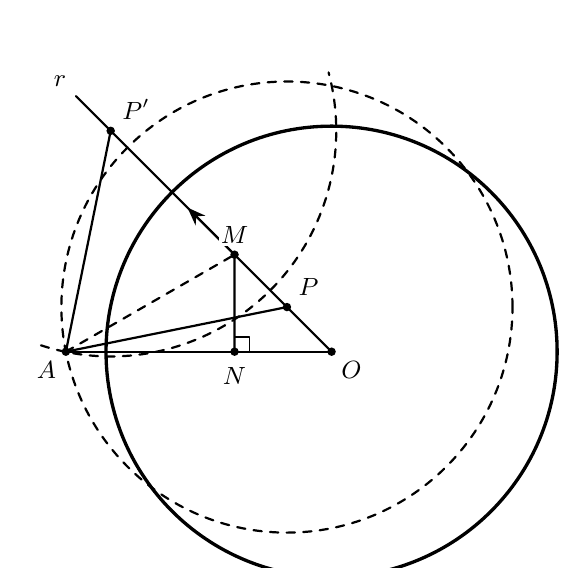
\begin{tikzpicture}[>=Stealth, scale=0.85, line cap=round, line join=round, font=\small]
  % Geometric scale: 1 unit = 60 km -> OA = 3.97, R = 3.37
  \coordinate (A) at (0, 0);
  \coordinate (O) at (3.97, 0);

  % Points along NW ray (135 deg) from O:
  % OM1 = 56.57 km -> 0.943; OM2 = 280.0 km -> 4.667
  \coordinate (P) at ($(O)+(135:0.943)$);
  \coordinate (M) at ($(O)+(135:2.05)$);
  \coordinate (Pprime) at ($(O)+(135:4.667)$);
  \coordinate (Rtip) at ($(O)+(135:5.4)$);
  \coordinate (N) at ($(M |- A)$);

  % Solid storm circle centered at O (radius R = 3.37, A is just outside)
  \draw[very thick] (O) circle (3.37);

  % Dashed storm circle centered at P (radius R = 3.37, passes through A)
  \draw[thick, dashed] (P) circle (3.37);

  % Dashed storm arc centered at P' (radius R = 3.37, passes through A)
  \draw[thick, dashed] ($(Pprime)+(-108:3.37)$) arc (-108:15:3.37);

  % Northwest ray r from O with mid-ray direction arrow
  \draw[thick] (O) -- (Rtip);
  \draw[->, thick] (M) -- ($(M)!0.38!(Pprime)$);

  % Segments OA, PA, P'A, MN (solid) and MA (dashed)
  \draw[thick] (A) -- (O);
  \draw[thick] (A) -- (P);
  \draw[thick] (A) -- (Pprime);
  \draw[thick] (M) -- (N);
  \draw[thick, dashed] (A) -- (M);

  % Right angle at N (on O-side, matching original scan)
  \draw (N) rectangle ++(0.22, 0.22);

  % Points and labels
  \fill (A) circle (1.8pt) node[below left] {$A$};
  \fill (O) circle (1.8pt) node[below right] {$O$};
  \fill (N) circle (1.8pt) node[below=2pt] {$N$};
  \fill (M) circle (1.8pt) node[above=3pt, fill=white, inner sep=0.8pt] {$M$};
  \fill (P) circle (1.8pt) node[above right=1pt] {$P$};
  \fill (Pprime) circle (1.8pt) node[above right=1pt] {$P'$};
  \node[above left] at (Rtip) {$r$};
\end{tikzpicture}
\caption{颱風路徑與暴風圈交會幾何分析}
\label{fig:b3-fig1-2}
\end{figure}

取 $P$ 與 $P'$ 為颱風眼進行路徑上距 $A$ 正好為 202 公里的兩個位置，即 $\overline{PA} = \overline{P'A} = 202$，此時，$(202)^2 = 400t^2 - 4760\sqrt{2}t + 56644$

整理一下得：
\begin{equation}
10t^2 - 119\sqrt{2}t + 396 = 0 \label{eq:b3-ch1-typhoon}
\end{equation}
即 $t$ 有兩解 $t = 2\sqrt{2}$ 或 $9.9\sqrt{2}$（即 $t = 2.83$ 或 $14.00$）。

換句話說，本地約清晨 4 時 50 分會進入暴風圈，到下午 4 時左右可望脫離。

這個問題的整個處理過程，便是把颱風的實際問題，先轉化成幾何經圖解後利用學過的畢氏定理化成代數上的方程式\eqref{eq:b3-ch1-typhoon}的求解，亦即相似而一般的問題，（假定 $O$ 不在 $A$ 點之正東方，且由經緯度標示 $A, O$ 兩點位置。又假定颱風進行方向不正好是西北方，可能是 $53^\circ 15'$ 這樣一個不太單純的方位）須賴座標與向量幾何引入之後才便於處理。\hfill \raisebox{-0.5ex}{\#}

\phantomsection\label{note:b3-ch1-p7-flowchart-sqrt2}%
\begin{center}
\begin{tikzpicture}[>=Stealth, line cap=round, line join=round, font=\small]
  \node[align=center] (real) at (0, 2.4) {\textbf{求何時落入及}\\\textbf{脫離暴風圈問題}};
  \node[align=center] (geom) at (6.5, 2.4) {\textbf{射線 $r$ 上點 $M$ 到一}\\\textbf{定點 $A$ 的距離問題}};
  \node[align=center] (alg) at (3.25, 0) {\textbf{解 $10t^2 - 119t + 396 = 0$}\footnotemark\\\textbf{之一元二次方程式}};

  \draw[->, thick] ([yshift=3pt]real.east) -- ([yshift=3pt]geom.west);
  \draw[<-, thick] ([yshift=-3pt]real.east) -- ([yshift=-3pt]geom.west);

  \draw[->, thick] ([xshift=-5pt]geom.south) -- ([xshift=10pt]alg.north);
  \draw[<-, thick] ([xshift=5pt]geom.south) -- node[below right, xshift=6pt, yshift=2pt] {直觀幾何（主要是畢氏定理）} ([xshift=20pt]alg.north);
\end{tikzpicture}
\end{center}
\footnotetext{【校訂註】原書流程圖代數方框中排印為「$10t^2 - 119t + 396 = 0$」，一次項係數漏印根號 $\sqrt{2}$（前文式 \eqref{eq:b3-ch1-typhoon} 明確為 $10t^2 - 119\sqrt{2}t + 396 = 0$）。正文照原印字樣錄入並在此校記。}

另一方面也存在著一些本身就是幾何的自然界問題。

\begin{example}
假設已有一圓筒狀的巨形水槽，欲建築一正立方水槽，使容量為圓筒水槽的 8 倍，求此正立方槽邊長若干。（這一類的問題就引發了各種體積的一系統的求算，同時也還要通過上述的過程，或利用直觀幾何或利用座標幾何，把水槽大小數量化為體積後，變成代數方程求解問題。）

若已知圓筒水槽底面積為 18 平方公尺，高為 12 公尺，則圓筒體積數量化後知為 $12 \times 18$ 立方公尺，亦即
\[ \text{圓筒容量} = \text{圓筒體積} = 18\text{ 平方公尺} \times 12\text{ 公尺} = 216\text{ 立方公尺}. \]
另一方面，設 $x$ 為正方水槽的邊長，則水槽大小數量化為體積後知為 $x^3$，故問題轉化為代數方程的求解問題，
即
\begin{align*}
x^3 &= \text{正立方水槽裝水量} = \text{圓筒水槽裝水量} \times 8 \\
    &= 216 \times 8 \text{（立方公尺）}
\end{align*}
即 $x^3 = 1728$（立方公尺）

故 $x = 12$（公尺）
\end{example}

這個過程也可圖示如下：

\begin{center}
\begin{tikzpicture}[>=Stealth, line cap=round, line join=round, font=\small]
  \node[align=center] (real) at (0, 2.4) {\textbf{立方水槽問題}\\（自然界）};
  \node[align=center] (geom) at (6.2, 2.4) {\textbf{體積及其邊長關係}\\（幾何）};
  \node[align=center] (alg) at (3.1, 0) {\textbf{解一元三次方程式}\\（代數）};

  \draw[->, thick] ([yshift=3pt]real.east) -- ([yshift=3pt]geom.west);
  \draw[<-, thick] ([yshift=-3pt]real.east) -- ([yshift=-3pt]geom.west);

  \draw[->, thick] ([xshift=-5pt]real.south) -- ([xshift=-18pt]alg.north);
  \draw[<-, thick] ([xshift=4pt]real.south) -- ([xshift=-9pt]alg.north);

  \draw[->, thick] ([xshift=-4pt]geom.south) -- ([xshift=9pt]alg.north);
  \draw[<-, thick] ([xshift=5pt]geom.south) -- node[below right, align=left, xshift=6pt, yshift=4pt] {直觀幾何\\座標幾何} ([xshift=18pt]alg.north);
\end{tikzpicture}
\end{center}
\hfill \raisebox{-0.5ex}{\#}

總結以上的討論，可知要描寫自然，解釋自然，甚至推演有用有利於人類社會進步發展的種種結論，我們可以依藉幾何來圖解自然現象，使我們的觀察具體化，使我們對自然現象易於瞭解，易於推想一些未知。

另一方面，要能正確地推求未知，我們純靠視覺的幾何只有吃力不討好，且不能獲得一普遍的方法，來有系統地處理問題。古典平面幾何已經顯示給我們這一重大缺陷：證明或推求一特殊結論都要累積了前人的許多心血，才求得一特殊技巧。這樣嚴重地妨礙了科學的全面發展。

希耳伯特公理化幾何的出現，開闢了數學本身一條路徑。亦即在一探討中的體系裏，提鍊出一組最基本的性質，然後以這組精練的資料去推演這體系內的每一個已知或未知的事實。它的好處在於使一個複雜的體系（比如說，歐氏幾何）有一個很清楚的脈絡。可惜它的導引過程，還是太難控制，同時也不直接有助於實際問題的處理。我們把它放在附錄裏。

有系統地轉化成為代數，利用代數的運算來推演，這是十七世紀以來所發現的重要路徑，在高中課程裏，我們將敘述沿依這路徑的兩個主流：座標幾何與向量幾何。

這兩道主流，在處理問題上，有時前者優於後者，有時後者優於前者。一開始我們將分別在第三、四兩章發展它們，但等到有點基礎以後，我們將揉合運用，不強分彼此。

其實，我們並不想完全忘卻古典平面幾何的好處。在古典平面幾何裏，可以說幾乎所有結論都來自「全等三角形定理」，畫補助線，將三角形搬來搬去，得到一些比較性的結論。這中間我們不忘一樣好處：在一些相當直觀的情況下，我們值得保留利用古典平面幾何去處理問題，這點在第五章 §5-3 中，我們要加以申述。

把以上的觀點，圖示於下：

\phantomsection\label{note:b3-ch1-p9-hilbert-name}%
\begin{center}
\begin{tikzpicture}[>=Stealth, line cap=round, line join=round, font=\small]
  \node[draw, rounded corners=2pt, minimum width=2.4cm, minimum height=1.1cm, align=center] (real) at (0, 2.6) {自然或人文\\的實際現象};
  \node[draw, rounded corners=2pt, minimum width=1.8cm, minimum height=1.1cm, align=center] (geom) at (4.8, 2.6) {幾\quad 何};
  \node[draw, rounded corners=2pt, minimum width=1.8cm, minimum height=1.0cm, align=center] (alg) at (2.4, 0.1) {代\quad 數};

  % Real to geom
  \draw[->, thick] ([yshift=3pt]real.east) -- ([yshift=3pt]geom.west);
  \draw[<-, thick] ([yshift=-3pt]real.east) -- ([yshift=-3pt]geom.west);

  % Real to alg
  \draw[->, thick] ([xshift=-5pt]real.south) -- ([xshift=-16pt]alg.north);
  \draw[<-, thick] ([xshift=4pt]real.south) -- ([xshift=-8pt]alg.north);

  % Geom to alg arrows
  \draw[->, thick] ([xshift=-4pt]geom.south) -- ([xshift=8pt]alg.north);
  \draw[<-, thick] ([xshift=5pt]geom.south) -- ([xshift=16pt]alg.north);

  % Self-loop on the right side of geom (matching original scan p. 9)
  \draw[->, thick] ([yshift=10pt]geom.east) .. controls (6.5, 3.0) and (6.5, 2.2) .. ([yshift=-10pt]geom.east);

  % Right side annotations as individual nodes
  \node[anchor=west, align=left, font=\scriptsize] (n1) at (7.0, 3.0) {1. 希爾伯特 (Hilbert) 公理化幾何\footnotemark\\ \quad（柏克荷夫 (Birkhoff) 數量化公理幾何）};
  \node[anchor=west, align=left, font=\scriptsize] (n2) at (7.0, 1.9) {2. 直觀幾何（包含古典平面幾何）};
  \node[anchor=west, align=left, font=\scriptsize] (n3) at (7.0, 1.05) {3. 座標幾何（又名解析幾何）};
  \node[anchor=west, align=left, font=\scriptsize] (n4) at (7.0, 0.35) {4. 向量幾何};

  % Brace grouping 3 & 4 (vertical along right edge of n3)
  \draw[decorate, decoration={brace, amplitude=4pt, raise=3pt}, thick]
    (n3.north east) -- (n3.east |- n4.south) node[midway, right=8pt, align=left, font=\scriptsize] {兩種系\\統轉化\\的過程};

  % Dashed pointer lines matching original scan p. 9
  \draw[dashed, thin] (n1.west) -- (6.25, 2.75);
  \draw[dashed, thin] (n2.west) -- (6.05, 2.25);
  \draw[dashed, thin] (n3.west) -- (4.35, 1.35);
  \draw[dashed, thin] (n4.west) -- (4.20, 1.15);
\end{tikzpicture}
\end{center}
\footnotetext{【校訂註】此處圖示項目 1 原印作「希爾伯特」，前文 p.~8 及附錄一標題均寫作「希耳伯特」，兩者為同一人名 David Hilbert 之不同漢字音譯，正文照原印字樣錄入。}

在上圖中，我們暫時忽略了以複數處理的平面上的幾何，這複數的體系是包含了實數系，猶如實數系之包含有理數系一樣，到第四冊，我們將見到複數如何與平面上的點一一對應，見到複數的完美與有力。

\subsubsection*{習題 1-1}

\begin{enumerate}[label=\arabic*., leftmargin=2em]
  \item 求一正立方體的邊長，使其體積為 216 立方米。
  \item 設一物體承受向下壓力 200 公斤，水平力 100 公斤，問它所受的合成力大小若干？（可利用勾股弦定理，即畢氏定理）。
  \begin{flushright}
  \begin{tikzpicture}[>=Stealth, scale=0.85, line cap=round, line join=round, font=\small, baseline=(current bounding box.center)]
    \draw[thick] (0, 0) circle (4pt);
    \draw[->, very thick] (0, 2.1) -- (0, 0.16) node[midway, right=2pt] {200公斤};
    \draw[->, very thick] (1.85, 0) -- (0.16, 0) node[midway, above=2pt, xshift=4pt] {100公斤};
    \draw[dashed, ->, thick] (-0.08, -0.14) -- (-0.95, -1.85) node[midway, left=3pt] {$?$};
  \end{tikzpicture}
  \end{flushright}
  \item 有一定長鐵絲網要圍成一個方形的場地，試證面積最大時，此場地必為正方形。\\
  （提示：應用二次函數的極大極小，第二冊第一章）
  \item 今有一高射砲，砲管與水平夾角為 $60^\circ$，砲彈出砲口時的初速為 600 公尺/秒，若將空氣阻力不計，試求彈道最高點與水平距離。〔注意：砲彈的水平位移 $x = v_1 t$，鉛垂位移 $y = -\frac{1}{2}gt^2 + v_2 t$，如圖所示 $v_1, v_2$ 分別為初速度的水平鉛垂分量〕
\end{enumerate}

\begin{figure}[H]
\centering
\begin{tikzpicture}[>=Stealth, scale=1.05, line cap=round, line join=round, font=\small]
  % Ground line
  \draw[thick] (-0.3, 0) -- (7.0, 0);

  % Parabola trajectory
  \draw[very thick] (0, 0) parabola bend (3.2, 2.8) (4.9, 2.0);
  \draw[very thick, dashed] (4.9, 2.0) parabola[bend at start] (6.4, 0);

  % Initial velocity rectangle and vector (v1 horizontal, v2 vertical)
  \draw[->, very thick] (0, 0) -- (1.15, 1.95);
  \draw[thick] (0, 0) rectangle (1.15, 1.95);
  \node[left=2pt] at (0, 1.0) {$v_2$};
  \node[below=1pt] at (0.58, 0) {$v_1$};
  \draw[->, thin] (0.5, 2.7) node[above] {初速度} -- (0.65, 1.35);

  % Peak pointer and gravity arrow
  \fill (3.2, 2.8) circle (1.8pt);
  \draw[->, thin] (3.95, 3.25) node[right] {彈道最高點} -- (3.3, 2.86);
  \draw[->, very thick] (3.2, 2.2) -- (3.2, 1.35) node[below] {$-mg$};

  % Sample point P for x and y braces (matching original scan p. 10)
  \coordinate (P) at (4.9, 2.0);
  \fill (P) circle (1.5pt);
  \draw[thick] (P) -- (4.9, 0);
  \draw[decorate, decoration={brace, amplitude=5pt, raise=3pt}, semithick]
    (4.9, 2.0) -- (4.9, 0) node[midway, right=8pt] {$y$};
  \draw[decorate, decoration={brace, mirror, amplitude=5pt, raise=13pt}, semithick]
    (0, 0) -- (4.9, 0) node[midway, below=18pt] {$x$};
\end{tikzpicture}
\caption{彈道拋物線運動分解}
\label{fig:b3-projectile}
\end{figure}

\subsection{座標幾何與向量幾何的比較}
\label{subsec:b3-1-2}

在第一、二冊裏，我們已發展了整數系，有理數系及實數系。這些數系及其基本運算，將提供我們一個有力的推演工具。

\subsubsection*{甲、座標幾何}

\begin{figure}[H]
\centering
\begin{minipage}{0.42\textwidth}
\centering
\begin{tikzpicture}[scale=0.9, line cap=round, line join=round, font=\small]
  % Rectangle ABCD
  \coordinate (A) at (0, 0);
  \coordinate (B) at (4.2, 0);
  \coordinate (C) at (4.2, 2.6);
  \coordinate (D) at (0, 2.6);
  \draw[thick] (A) rectangle (C);

  \node[below left] at (A) {$A$};
  \node[below right] at (B) {$B$};
  \node[above right] at (C) {$C$};
  \node[above left] at (D) {$D$};

  % Fly position
  \coordinate (Fly) at (1.7, 1.0);
  \fill (Fly) circle (1.8pt);
  \draw[dashed] (Fly) -- (1.7, 0) node[midway, right=2pt] {1公寸};
  \draw[dashed] (Fly) -- (0, 1.0) node[midway, above=2pt] {2公寸};
\end{tikzpicture}
\caption{桌面蒼蠅位置座標化}
\label{fig:b3-fig1-3}
\end{minipage}
\hfill
\begin{minipage}{0.53\textwidth}
例如：桌面上一隻蒼蠅，你告訴我它距左緣 ($AD$) 2 公寸，距下緣 ($AB$) 1 公寸，那麼我就很清楚的可找到它，因此蒼蠅的位置可以用一對數 $(2, 1)$ 來表示它。
\end{minipage}
\end{figure}

座標幾何，便是把平面的點適當地以兩個實數來描寫（空間的點則以三個實數來描寫），這個描寫的方法其實在國中已經學過。也就是說，在平面上任取一點 $O$，固定它，然後取兩條通過 $O$ 點而相互垂直的有向直線作為平面上的兩個軸，分別稱為 $X$ 軸，$Y$ 軸，如圖 1-4.

\begin{figure}[H]
\centering
\begin{tikzpicture}[>=Stealth, scale=1.1, line cap=round, line join=round, font=\small]
  \draw[->, thick] (-1, 0) -- (5, 0) node[right] {$X$};
  \draw[->, thick] (0, -1) -- (0, 3.5) node[above] {$Y$};
  \node[below left] at (0, 0) {$O$};

  \coordinate (P) at (3.2, 2.4);
  \fill (P) circle (2pt) node[above right] {$P$};
  \draw[dashed, thick] (P) -- (3.2, 0) node[below] {$Q$};
  \draw[dashed, thick] (P) -- (0, 2.4) node[left] {$R$};
\end{tikzpicture}
\caption{笛卡兒直角座標系}
\label{fig:b3-fig1-4}
\end{figure}

現在 $X$ 軸，$Y$ 軸本身各別都與實數系一一對應\footnote{一一對應即相當於我們在第二冊第四章所講函數的對射性。}，使 $O$ 點都對應於零。因此對平面上任一點 $P$，分別由 $P$ 向 $X$ 及 $Y$ 軸作垂線，設垂足為 $Q, R$ 兩點，記 $Q$ 點在 $X$ 軸所相應的實數為 $x$，稱為 $P$ 在 $X$ 軸的成分，同樣記 $R$ 點在 $Y$ 軸所相應的實數為 $y$，稱為 $P$ 在 $Y$ 軸的成分。這兩樣成分 $x, y$ 按序記成 $(x, y)$。這樣 $P$ 與一對實數 $(x, y)$ 間的對應是一一的，因兩對實數 $(x, y)$ 與 $(x', y')$，若不是 $x = x'$ 且 $y = y'$，其所代表的點 $P$ 與 $P'$ 必然不同。

\begin{figure}[H]
\centering
\begin{minipage}{0.48\textwidth}
\centering
\begin{tikzpicture}[>=Stealth, scale=0.95, line cap=round, line join=round, font=\small]
  \draw[->, thick] (-0.8, 0) -- (4.5, 0) node[right] {$X$};
  \draw[->, thick] (0, -0.5) -- (0, 3.5) node[above] {$Y$};
  \node[below left] at (0, 0) {$O$};

  \coordinate (P) at (2.2, 2.2);
  \coordinate (Pprime) at (3.5, 1.2);
  \fill (P) circle (2pt) node[above right] {$P$};
  \fill (Pprime) circle (2pt) node[above right] {$P'$};

  \draw[dashed] (P) -- (2.2, 0) node[below] {$x$};
  \draw[dashed] (P) -- (0, 2.2) node[left] {$y$};
  \draw[dashed] (Pprime) -- (3.5, 0) node[below] {$x'$};
  \draw[dashed] (Pprime) -- (0, 1.2) node[left] {$y'$};
\end{tikzpicture}
\caption{$x \ne x'$ 且 $y \ne y'$}
\label{fig:b3-fig1-5}
\end{minipage}
\hfill
\begin{minipage}{0.48\textwidth}
\centering
\begin{tikzpicture}[>=Stealth, scale=0.95, line cap=round, line join=round, font=\small]
  \draw[->, thick] (-0.8, 0) -- (4.5, 0) node[right] {$X$};
  \draw[->, thick] (0, -0.5) -- (0, 3.5) node[above] {$Y$};
  \node[below left] at (0, 0) {$O$};

  \coordinate (P) at (2.8, 2.5);
  \coordinate (Pprime) at (2.8, 1.2);
  \fill (P) circle (2pt) node[above right] {$P$};
  \fill (Pprime) circle (2pt) node[above right] {$P'$};

  \draw[dashed] (P) -- (2.8, 0) node[below] {$x=x'$};
  \draw[dashed] (P) -- (0, 2.5) node[left] {$y$};
  \draw[dashed] (Pprime) -- (0, 1.2) node[left] {$y'$};
\end{tikzpicture}
\caption{$x = x'$ 但 $y \ne y'$}
\label{fig:b3-fig1-6}
\end{minipage}
\end{figure}

上圖顯示，兩對實數只要有第一個成分或第二個成分不等，如 $y \ne y'$（縱然 $x = x'$，如圖 1-6），則所代表的點 $P$ 與 $P'$ 便不相同，有了這個對應，我們稱 $(x, y)$ 為 $P$ 的座標，（或笛卡兒座標）。

座標幾何的用意便是根據上述點與座標的對應把幾何的對象，如直線拋物線兩直線的交點等各色各樣的圖形轉化成代數的對象，如直線轉化成一次方程，拋物線轉化成的二次方程，而兩直線的交點轉化成聯立的兩個一次方程的解。

這個轉化是系統性的轉化，經過這轉化後，問題變成代數上的處理，第一、二冊裏我們已學會相當程度的代數推演方法，這樣的轉化處理，便是座標幾何（亦名解析幾何 analytic geometry）的精神，這是笛卡兒的一大貢獻。

\subsubsection*{乙、向量幾何}

至於向量幾何，則是把空間中（或平面上）任一點 $P$ 先看成一個以固定原點 $O$ 為起點，以 $P$ 為終點的有向線段 $\vec{OP}$（稱之為向量），於是空間中（或平面上）的所有點便與所有這樣的向量形成一個良好的一一對應。然後我們更准許向量 $\vec{OP}$ 可以到處平移，而仍看成同一向量，亦即圖中

\begin{figure}[H]
\centering
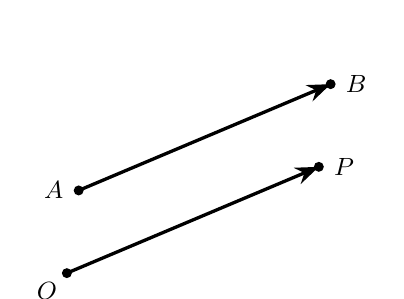
\begin{tikzpicture}[>=Stealth, scale=1.0, line cap=round, line join=round, font=\small]
  % Vector OP (no background grid/axes; original scan p. 12 only has the two vectors)
  \coordinate (O) at (0, 0);
  \coordinate (P) at (3.2, 1.35);
  \draw[->, very thick] (O) -- (P);
  \fill (O) circle (1.8pt) node[below left] {$O$};
  \fill (P) circle (1.8pt) node[right=2pt] {$P$};

  % Translated Vector AB
  \coordinate (A) at (0.15, 1.05);
  \coordinate (B) at (3.35, 2.40);
  \draw[->, very thick] (A) -- (B);
  \fill (A) circle (1.8pt) node[left=2pt] {$A$};
  \fill (B) circle (1.8pt) node[right=2pt] {$B$};
\end{tikzpicture}
\caption{向量之平移等價性}
\label{fig:b3-fig1-7}
\end{figure}

$\vec{AB}$ 與 $\vec{OP}$ 雖然作為有向線段來說顯然是不同的兩個東西，但看成向量，我們就不加以區分，也就是說，作為向量來看，$\vec{AB}$ 與 $\vec{OP}$ 是代表同一向量，這個道理是因為我們考慮向量時，只考慮一個如下的口令“朝哪個方向前進多遠”而不計較起點，一個向量便相當於一個這樣的口令，（執行口令皆是可以不知自己原來身在何處，只要有了羅盤針及距離表便可以照做）。

要使問題經過向量幾何的轉化後能夠用推演處理，便須充實向量間的運算構造，我們將適當引入向量的加、減、係數積、內積（及外積），以後我們可以看到許多問題轉化成向量的問題後如何利用這些運算來推求未知。很多時候，向量處理要比座標處理優越，但嚴格說來，向量的運算還是奠定在座標成分的實數系運算上，只是較為簡化符號且授予更清晰的幾何意義。

總結一下：

\textbf{座標幾何}\quad 平面（或空間）的點可由其笛卡兒座標來描述。而笛卡兒座標的成分（平面上有兩個成分，空間中則需三個）不過是實數。如此利用實數系的代數運算可推演平面上（或空間中）各種已知或未知的事實。

\textbf{向量幾何}\quad 平面（或空間）的點可由向量（的尾端）來描述。所有向量自成一個可運算的代數體系（這代數體系中的特別構造如內積（§3-5），外積（第四冊），一方面有它直觀的幾何意義，另一方面又可表成諸向量的座標成分，利用實數系的運算來表示），這代數體系提供了處理與推演的大好場地。

\subsubsection*{習題 1-2}

\begin{enumerate}[label=\arabic*., leftmargin=2em]
  \item 通常圍棋盤兩邊各 19 目（也就是 18 方格，棋子放在「目」即交點上）。假想有一棋局正在進行，試給一座標系，以座標描述其第一手到第六手。
  \item 國中物理課講力與運動時就介紹了力的合成與分解試把力的要素及其運算等有關的觀念用圖表示。
\end{enumerate}

\subsection{代數工具的複習提要}
\label{subsec:b3-1-3}

在一、二冊中我們已很辛苦地完成了實數系的建構，練習並瞭解了實數間的運算及性質。

另一方面，世間各種現象常以函數的形式出現，簡單的像
\begin{enumerate}[label=(\arabic*), leftmargin=2em]
  \item 華氏與攝氏溫度的換算：
  \[ y = \frac{9}{5}x + 32 \]
  其中 $x$ 表攝氏度數，$y$ 表華氏度數。
  \item 質點的等速直線運動：
  \[ y = vx \]
  其中 $x$ 表時間，$y$ 為位移，$v$ 為速度，皆為一次函數。
\end{enumerate}

稍複雜的像彈道，便以二次函數來描述，然後我們考慮過一般高次多項式函數：
\[ y = a_0 x^n + a_1 x^{n-1} + \dots + a_{n-1} x + a_n \quad (a_0 \ne 0) \]
更考慮過有理函數，即兩多項式之商，我們知道這些函數間如何運算，也知道所相應的一次方程，二次方程，甚至聯立方程，如何求解。

進一步，為了把乘法變成加法，使計算尺能計算乘法，除法，我們引進來對數函數 $\log_a$，知有
\[ \log_a (uv) = \log_a u + \log_a v;\quad 1 \ne a > 0 \text{ 而 } u, v > 0 \]
對數函數的反函數，則為指數函數。

我們將在第二章中再以三角測量為問題核心，引入三角函數。

這樣，我們大體完備了所需要的函數。（在進一步的數學課程裏，由於極限觀念的大量運用，我們將以“逼近”，探討表為更複雜的函數之自然或人文現象。）

以後各章中，我們將按本章所述處理實際問題的原則，剖析座標幾何、向量幾何的轉化過程，使同學能把實際問題（經由幾何）化成代數問題，而利用我們所學的代數工具去推演有用有利於社會發展的各種結論。

\subsubsection*{習題 1-3}

\begin{enumerate}[label=\arabic*., leftmargin=2em]
  \item 試將高一所學過的各個代數體系，如自然數系，整數系有理數系實數系的基本運算，即加法與乘法個別整理出來。
  \item 將力的合成與實數的加法所各具有的性質做一比較。
  \item 將計算尺原理做一大略說明（複習第二冊第五章）。
\end{enumerate}
 % 第一章 實際世界——幾何與代數
% =========================================================================
% 《高中數學實驗教材》第三冊（自然組）
% 第二章 直觀幾何與三角函數
% =========================================================================

\section{直觀幾何與三角函數}
\label{sec:b3-ch2}

\begin{center}
\begin{minipage}{0.65\textwidth}
\begin{itemize}[leftmargin=2em, itemsep=0.3em]
  \item[§2-1] 有向線段與有向角
  \begin{itemize}[leftmargin=2em, itemsep=0.2em]
    \item[甲、] 有向角
    \item[乙、] 無向角
    \item[丙、] 有向角的推廣
    \item[丁、] 角的記號
    \item[戊、] 同界角
    \item[己、] 角度的單位
    \item[庚、] 扇形
  \end{itemize}
  \item[§2-2] 三角函數的定義
  \begin{itemize}[leftmargin=2em, itemsep=0.2em]
    \item[甲、] 銳角的三角函數
    \item[乙、] 三角函數
  \end{itemize}
  \item[§2-3] 一些簡易的恒等式
  \item[§2-4] 一些幾何上量的定理
  \begin{itemize}[leftmargin=2em, itemsep=0.2em]
    \item[甲、] 畢氏定理的推廣
    \item[乙、] 三角形之面積與邊長
  \end{itemize}
  \item[§2-5] 三角測量
\end{itemize}
\end{minipage}
\end{center}

\begin{center}
$* \qquad * \qquad * \qquad * \qquad *$
\end{center}

國中教科書上已學過直線、三角形、平行四邊形與圓等的一些幾何圖形的基本性質，同時也提過利用銳角三角函數去作一些簡易的測量。

我們假定對那些學過的東西已相當熟悉，而要利用本章的篇幅進一步作更細膩的申述，以方便以後的用途。同時利用這些剛發展出來的三角函數的工具應用到測量上去，趁此也再一次說明了第一章中所提實際問題、幾何與代數間的轉化關係。

我們將討論一般廣義角的三角函數來代替國中考慮的特殊情形：銳角的三角函數。這樣一來我們才能廣泛推展三角函數間的運算。

\subsection{有向線段與有向角}
\label{subsec:b3-2-1}

\subsubsection*{甲、有向角}

有甲乙兩地，由甲地引到乙地的\textbf{有向線段}，可以看成是乙地相對於甲地位置的一種描寫。一個有向線段依它的「始點」「方向」「長度」而決定，比如，「自甲地向東北方走 5 公里」此時始點是甲地，方向是東北向，長度是 5 公里。這樣便得到乙地，且描寫出來乙地相對於甲地的位置。

\begin{figure}[H]
\centering
\begin{tikzpicture}[>=Stealth, scale=0.9, font=\small]
  \coordinate (A) at (0, 0);
  \coordinate (B) at (3.5, 2.5);
  \draw[->, very thick] (A) -- (B) node[midway, above left, sloped] {5公里};
  \fill (A) circle (2pt) node[below left] {甲地};
  \fill (B) circle (2pt) node[right] {乙地};
\end{tikzpicture}
\caption{有向線段}
\label{fig:b3-fig2-1}
\end{figure}

同樣地把上述「相對位置」的考慮改成「相對方位」的考慮，我們將得到所謂有向角。

地理或航海上，我們慣於使用「方位」的字眼來代替「方向」。設平面上有甲、乙兩種方位，若已知甲方位，欲求乙方位，我們便須知道乙方位相對於甲方位的「相對方位」或「方位差」，例如：乙方位乃由甲方位按逆時針方向旋轉 $120^\circ$ 而得。比照於有向線段，我們引進來\textbf{有向角}的觀念，它由下列三個因素組成：

「始邊」「旋轉方向」「旋轉量」

就如在上述例子中，始邊是甲方位，旋轉方向是逆時針方向，旋轉量則為 $120^\circ$。

\begin{figure}[H]
\centering
\begin{tikzpicture}[>=Stealth, scale=0.9, line cap=round, line join=round, font=\small]
  \coordinate (O) at (0, 0);
  \draw[->, very thick] (O) -- (-35:2.8) node[below right] {甲方位};
  \draw[->, very thick] (O) -- (85:2.8) node[right] {乙方位};
  \draw[->, thick] (-35:0.9) arc (-35:85:0.9) node[midway, right=2pt] {$120^\circ$};
  \fill (O) circle (1.5pt);
\end{tikzpicture}
\caption{有向角方位示意}
\label{fig:b3-fig2-2}
\end{figure}

平面上的有向角，其可能的旋轉方向只有逆時針與順時針兩個方向，我們用正負向來區別它們：規定逆時針旋轉便是正向，順時針旋轉便是負向，並據此將正號或負號記在旋轉量之前，稱為有向角的角度。換句話說，有向角的旋轉方向及旋轉量合併起來，稱為有向角的角度。像上例的有向角，角度為 $+120^\circ$，或簡記為 $120^\circ$（但負號不能省略）。又如圖 2-3：

\begin{figure}[H]
\centering
\begin{minipage}{0.48\textwidth}
\centering
\begin{tikzpicture}[>=Stealth, scale=0.9, line cap=round, line join=round, font=\small]
  \coordinate (O) at (0, 0);
  \draw[->, very thick] (O) -- (60:2.5) node[above] {乙方位};
  \draw[->, very thick] (O) -- (120:2.5) node[above] {甲方位};
  \draw[->, thick] (120:0.85) arc (120:60:0.85);
  \node[above=2pt] at (90:0.95) {$-60^\circ$};
\end{tikzpicture}
\end{minipage}
\hfill
\begin{minipage}{0.48\textwidth}
\centering
\begin{tikzpicture}[>=Stealth, scale=0.9, line cap=round, line join=round, font=\small]
  \coordinate (O) at (0, 0);
  \draw[->, very thick] (O) -- (90:2.5) node[left] {甲方位};
  \draw[->, very thick] (O) -- (-150:2.5) node[below right] {乙方位};
  \draw[->, thick] (90:0.75) arc (90:-150:0.75);
  \node[right=2pt] at (-30:0.85) {$-240^\circ$};
\end{tikzpicture}
\end{minipage}
\caption{負向旋轉之有向角}
\label{fig:b3-fig2-3}
\end{figure}

左圖有向角之角度記為 $-60^\circ$，右圖則記以 $-240^\circ$。

這樣一個有向角可由它的「始邊」與「角度」來決定，另一方面，也可由它的「始邊」「旋轉方向」「終邊」來決定。（即以「終邊」代替上述的「旋轉量」）。例如圖 2-4 中，若確知始邊為正北方位，終邊為東南方位，而旋轉方向為負向（即順時針方向），則旋轉量知為 $135^\circ$。反過來，若確知始邊為正北，旋轉方向為負向，而旋轉量為 $135^\circ$，則終邊知為東南方位。

\begin{figure}[H]
\centering
\begin{tikzpicture}[>=Stealth, scale=0.9, line cap=round, line join=round, font=\small]
  \draw[->, very thick] (0, 0) -- (0, 2.8) node[above] {$N$ 正北方位};
  \draw[->, very thick] (0, 0) -- (-45:2.8) node[below right] {東南方位 $SE$};
  \draw[->, thick] (90:0.85) arc (90:-45:0.85) node[midway, right=2pt] {$-135^\circ$};
  \draw[->, thick, dashed] (90:1.25) arc (90:315:1.25) node[midway, left=2pt] {$225^\circ$};
\end{tikzpicture}
\caption{方位角旋轉對照}
\label{fig:b3-fig2-4}
\end{figure}

\subsubsection*{乙、無向角}

國中講過的「角」，其實就是將上述的有向角，不分其兩邊誰始誰終，只考慮角的兩邊，也因此不分其旋轉方向是正是負，只管旋轉後留下的痕跡。這樣的角，在必要區別時，我們特稱為\textbf{無向角}，平常仍沿稱為角。無向角的角度便是它張角的大小，永遠不為負值。

圖 2-5 左側兩個有向角都對應到同一個畫在右側的無向角。

\begin{figure}[H]
\centering
\begin{tikzpicture}[>=Stealth, scale=0.85, line cap=round, line join=round, font=\small]
  % Left 1: +120
  \coordinate (O1) at (0, 0);
  \draw[->, thick] (O1) -- (-45:2.1) node[right] {始邊};
  \draw[->, thick] (O1) -- (75:2.1) node[right] {終邊};
  \draw[->, thick] (-45:0.75) arc (-45:75:0.75) node[midway, right=2pt] {$120^\circ$};

  \node at (2.8, 0.3) {與};

  % Left 2: -120
  \coordinate (O2) at (4.2, 0);
  \draw[->, thick] (O2) -- ($(O2)+(75:2.1)$) node[right] {始邊};
  \draw[->, thick] (O2) -- ($(O2)+(-45:2.1)$) node[right] {終邊};
  \draw[->, thick] ($(O2)+(75:0.75)$) arc (75:-45:0.75) node[midway, right=2pt] {$-120^\circ$};

  \draw[->, very thick] (7.0, 0.3) -- (8.0, 0.3);

  % Right: Undirected 120
  \coordinate (O3) at (9.3, 0);
  \draw[thick] (O3) -- ($(O3)+(-45:2.1)$);
  \draw[thick] (O3) -- ($(O3)+(75:2.1)$);
  \draw ($(O3)+(-45:0.75)$) arc (-45:75:0.75) node[midway, right=2pt] {$120^\circ$};
\end{tikzpicture}
\caption{有向角與無向角之對應 (一)}
\label{fig:b3-fig2-5-1}
\end{figure}

\begin{figure}[H]
\centering
\begin{tikzpicture}[>=Stealth, scale=0.85, font=\small]
  % Left 1: -240
  \coordinate (O1) at (0, 0);
  \draw[->, thick] (O1) -- (1.8, -1.2) node[right] {始邊};
  \draw[->, thick] (O1) -- (0.5, 2) node[above] {終邊};
  \draw[->, thick] (0.8, -0.5) arc (-33:247:0.9) node[midway, left] {$-240^\circ$};

  \node at (2.5, 0.5) {與};

  % Left 2: +240
  \coordinate (O2) at (4, 0);
  \draw[->, thick] (O2) -- (4.5, 2) node[above] {始邊};
  \draw[->, thick] (O2) -- (5.8, -1.2) node[right] {終邊};
  \draw[->, thick] (4.5, 0.8) arc (76:307:0.9) node[midway, left] {$240^\circ$};

  \draw[->, very thick] (6.8, 0.5) -- (7.8, 0.5);

  % Right: Undirected 240
  \coordinate (O3) at (9.5, 0);
  \draw[thick] (O3) -- (11.3, -1.2);
  \draw[thick] (O3) -- (10, 2);
  \draw (10.3, -0.4) arc (-33:247:0.9) node[midway, left] {$240^\circ$};
\end{tikzpicture}
\caption{有向角與無向角之對應 (二)}
\label{fig:b3-fig2-5-2}
\end{figure}

給了兩邊，我們取它所夾的兩個角中的較小的那一個無向角，稱為這兩邊的\textbf{夾角}.〔當這邊所代表的兩條射線方向正好相反時，必須再另外指定所取的夾角是哪一個無向角〕這兩邊則稱為這個無向角的兩個夾邊。

\subsubsection*{丙、有向角的推廣}

在第一章我們提過，若約定一個基準點 $O$，則空間（或平面上）任一點 $P$ 的位置，可由其相應的有向線段 $\vec{OP}$ 來決定。同樣我們約定一基準方位 $\mathbf{r}_0$，〔習慣上，作圖時取之為地圖上的東向，這相當於慣常我們沿一座標系 $(O; X, Y)$ 繪出的 $OX$ 軸方向〕，使得任一方位 $\mathbf{r}$ 皆可由 $\mathbf{r}_0$ 繞到 $\mathbf{r}$ 的有向角之角度確定，如給定 $120^\circ$（或 $-240^\circ$）便可確定的正確方位。

\begin{figure}[H]
\centering
\begin{tikzpicture}[>=Stealth, scale=0.9, font=\small]
  \coordinate (O) at (0, 0);
  \draw[->, very thick] (O) -- (3.5, 0) node[right] {$X$（基準方位 $\mathbf{r}_0$）};
  \draw[->, very thick] (O) -- (120:3) node[above left] {$\mathbf{r}$};
  \draw[->, thick] (0.8, 0) arc (0:120:0.8) node[midway, above right] {$120^\circ$};
  \draw[->, thick, dashed] (1.1, 0) arc (0:-240:1.1) node[midway, below] {$-240^\circ$};
  \fill (O) circle (1.5pt) node[below left] {$O$};
\end{tikzpicture}
\caption{基準方位與角度定位}
\label{fig:b3-fig2-6}
\end{figure}

如果只一味要考慮「相對方位」或「方位差」，上述有向角的定義便已妥善無虞。但以後我們將會見到我們有需要不把有向角限制在 $-360^\circ$ 到 $+360^\circ$ 之間。很多時候，雖然我們繞了 $360^\circ$（或 $-360^\circ$）又回到原來的方位，但有些相關的狀況卻已改變。若把有向角看成是方位的旋轉本身，那麼一個磨穀的石磨仔旋轉一百圈後，回到原來的方位，與它從來不曾旋轉明顯有著區別。為了把這種區別顯示出來，我們要推廣有向角的定義：

\begin{figure}[H]
\centering
\begin{tikzpicture}[>=Stealth, scale=0.85, line cap=round, line join=round, font=\small]
  % Base tray of millstone
  \draw[thick] (-1.5, -0.4) arc (180:360:1.5 and 0.42);
  \draw[thick] (-1.5, -0.4) -- (-1.5, -0.05);
  \draw[thick] (1.5, -0.4) -- (1.5, -0.05);
  % Lower millstone
  \draw[thick] (-1.15, -0.05) arc (180:360:1.15 and 0.32);
  \draw[thick] (-1.15, -0.05) -- (-1.15, 0.35);
  \draw[thick] (1.15, -0.05) -- (1.15, 0.35);
  % Upper millstone
  \draw[thick, fill=white] (0, 0.75) ellipse (1.15 and 0.32);
  \draw[thick] (-1.15, 0.35) arc (180:360:1.15 and 0.32);
  \draw[thick] (-1.15, 0.35) -- (-1.15, 0.75);
  \draw[thick] (1.15, 0.35) -- (1.15, 0.75);
  % Top hopper hole & wooden pin
  \draw[thick] (-0.22, 0.78) ellipse (0.16 and 0.06);
  \draw[thick] (0.28, 0.80) ellipse (0.10 and 0.04);
  % Wooden handle sticking out to the right
  \draw[thick, fill=white] (1.05, 0.55) -- (2.55, 0.85) -- (2.55, 0.70) -- (1.05, 0.40) -- cycle;
  % Rotation indicator arrow
  \draw[->, thick, dashed] (1.9, 1.15) arc (35:145:1.2 and 0.45);
  \node[above] at (0.85, 1.38) {\scriptsize 旋轉方向};
\end{tikzpicture}
\caption{石磨旋轉示意（圖 2-7）}
\label{fig:b3-fig2-7}
\end{figure}

一個\textbf{廣義有向角}可以看成是一條射線的“單向”轉動（單向指在逆時針或順時針中取定一方向）其度量可由其旋轉方向及旋轉量來給定。與（狹義）有向角的情形一樣，它的度量稱為廣義有向角的角度，它可以是任意一個實數。

例如它可以是 $+780^\circ$ 或 $-510^\circ$，前者表示一條射線沿逆時針方向繞整整兩圈後接著又繞了 $60^\circ$ 的一個旋轉。（因 $780^\circ = 2\times 360^\circ + 60^\circ$）。後者表示一條射線沿順時針方向整整繞了一圈後，接著又繼續繞了 $150^\circ$ 角度的旋轉（因 $-510^\circ = (-1)\times 360^\circ + (-150^\circ)$）。

\begin{figure}[H]
\centering
\begin{minipage}{0.48\textwidth}
\centering
\begin{tikzpicture}[>=Stealth, scale=0.95, line cap=round, line join=round, font=\small]
  \coordinate (O) at (0, 0);
  \draw[->, very thick] (O) -- (60:2.5) node[above] {始邊};
  \draw[->, very thick] (O) -- (120:2.5) node[above] {終邊};
  \draw[->, thick, domain=0:780, samples=220, variable=\t]
    plot ({(0.22 + 0.00065*\t)*cos(\t+60)}, {(0.22 + 0.00065*\t)*sin(\t+60)});
  \draw[<->, thin] (60:1.25) arc (60:120:1.25);
  \node[fill=white, inner sep=1pt] at (90:1.52) {$60^\circ$};
  \node[below] at (0, -0.85) {$+780^\circ$};
\end{tikzpicture}
\caption{$+780^\circ$ 廣義旋轉角}
\label{fig:b3-fig2-8-1}
\end{minipage}
\hfill
\begin{minipage}{0.48\textwidth}
\centering
\begin{tikzpicture}[>=Stealth, scale=0.95, line cap=round, line join=round, font=\small]
  \coordinate (O) at (0, 0);
  \draw[->, very thick] (O) -- (60:2.5) node[above] {始邊};
  \draw[->, very thick] (O) -- (270:2.1) node[below] {終邊};
  \draw[->, thick, domain=0:510, samples=220, variable=\t]
    plot ({(0.25 + 0.00085*\t)*cos(60-\t)}, {(0.25 + 0.00085*\t)*sin(60-\t)});
  \node[right] at (0.85, -0.35) {$-510^\circ$};
  \node[above left] at (-0.65, 0.55) {$210^\circ$};
\end{tikzpicture}
\caption{$-510^\circ$ 廣義旋轉角}
\label{fig:b3-fig2-8-2}
\end{minipage}
\end{figure}

由於前述的有向角只不過是廣義有向角的特殊情形，（換句話說，有向角只不過是角度介於 $0^\circ$ 與 $360^\circ$ 之間的廣義有向角）。以後我們可以單單考慮廣義有向角，而把它略稱為有向角。

不管是（廣義）有向角或無向角，以後我們都沿依習慣，通稱為\textbf{角}. 必要區別時，我們再予明言。

\subsubsection*{丁、角的記號}

一個（廣義）有向角，角度 $\theta$（含旋轉方向與旋轉量）與始邊 $\mathbf{r}_1$ 確定後，這個有向角本身也就確定。有時為了特別要表明始終邊 $\mathbf{r}_1, \mathbf{r}_2$ 的位置，把這個有向角記成 $\angle(\theta; \mathbf{r}_1, \mathbf{r}_2)$，方便上簡記為 $\angle\theta$。注意這時 $\theta$ 可正可負，例如圖 2-9-1 中 $\theta = -35^\circ$。

\begin{figure}[H]
\centering
\begin{minipage}{0.48\textwidth}
\centering
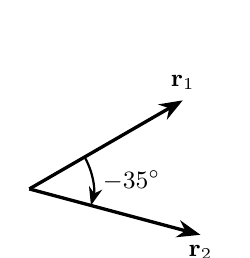
\begin{tikzpicture}[>=Stealth, scale=0.9, font=\small]
  \coordinate (O) at (0, 0);
  \draw[->, very thick] (O) -- (30:2.5) node[above] {$\mathbf{r}_1$};
  \draw[->, very thick] (O) -- (-15:2.5) node[below] {$\mathbf{r}_2$};
  \draw[->, thick] (30:0.9) arc (30:-15:0.9) node[midway, right] {$-35^\circ$};
\end{tikzpicture}
\caption{$\angle(\theta; \mathbf{r}_1, \mathbf{r}_2)$ 有向角}
\label{fig:b3-fig2-9-1}
\end{minipage}
\hfill
\begin{minipage}{0.48\textwidth}
\centering
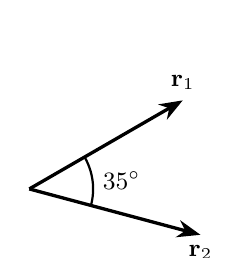
\begin{tikzpicture}[>=Stealth, scale=0.9, font=\small]
  \coordinate (O) at (0, 0);
  \draw[->, very thick] (O) -- (30:2.5) node[above] {$\mathbf{r}_1$};
  \draw[->, very thick] (O) -- (-15:2.5) node[below] {$\mathbf{r}_2$};
  \draw[thick] (30:0.9) arc (30:-15:0.9) node[midway, right] {$35^\circ$};
\end{tikzpicture}
\caption{無向角記號}
\label{fig:b3-fig2-9-2}
\end{minipage}
\end{figure}

同樣，一個無向角，我們也記為 $\angle\theta$。其中 $\theta$ 指它的角度，其值永不為負，例如圖 2-9-2 中 $\theta = 35^\circ$。

設 $\angle\theta$ 為 $\mathbf{r}_1, \mathbf{r}_2$ 的夾角，$\mathbf{r}_1, \mathbf{r}_2$ 上各有點 $B$ 與 $C$，且 $A$ 為 $\mathbf{r}_1$ 與 $\mathbf{r}_2$ 的公共端點（$A$ 稱為 $\angle\theta$ 的頂點），則 $\angle\theta$ 可記以
\[ \angle BAC \quad\text{或}\quad \angle CAB \]
以便於從圖上辨認，有時甚至略記為 $\angle A$。即
\[ \angle\theta \equiv \angle BAC \equiv \angle CAB \equiv \angle A \]

我們列一個表來整理一下上述種種，它只是用來比較上述繁雜的陳述與規約，並不是要用來記憶。

\begin{figure}[H]
\centering
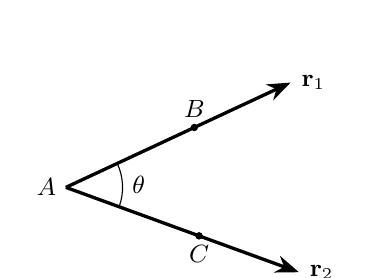
\begin{tikzpicture}[>=Stealth, scale=0.9, font=\small]
  \coordinate (A) at (0, 0);
  \draw[->, very thick] (A) -- (25:3.5) node[right] {$\mathbf{r}_1$};
  \draw[->, very thick] (A) -- (-20:3.5) node[right] {$\mathbf{r}_2$};
  \fill (25:2) circle (1.5pt) node[above] {$B$};
  \fill (-20:2) circle (1.5pt) node[below] {$C$};
  \draw (25:0.8) arc (25:-20:0.8) node[midway, right] {$\theta$};
  \node[left] at (A) {$A$};
\end{tikzpicture}
\caption{夾角與頂點記號}
\label{fig:b3-fig2-10}
\end{figure}

\begin{table}[H]
\centering
\footnotesize
\renewcommand{\arraystretch}{1.25}
\setlength{\tabcolsep}{4pt}
\resizebox{\textwidth}{!}{%
\begin{tabular}{|c|c|c|c|c|c|c|c|}
\hline
\multirow{2}{*}{\shortstack{有向\\線段}} & 概念 & 有向線段 & 位置 & 起點；終點 & 方向 & 長度 & 長度範圍 \\ \cline{2-8}
 & 記號 & $\vec{AB}$ & $A, B$ 等 & $A; B$ &  & $\overline{AB}$ & $0 \le \overline{AB}$ \\ \hline
\multirow{2}{*}{\shortstack{（廣義）\\有向角}} & 概念 & 有向角 & 方位 & 始邊；終邊 & 旋轉方向 & 角度 & 角度範圍 \\ \cline{2-8}
 & 記號 & \shortstack{$\angle(\theta; \mathbf{r}_1, \mathbf{r}_2)$\\或 $\angle\theta$} & $\mathbf{r}_1, \mathbf{r}_2$ 等 & $\mathbf{r}_1; \mathbf{r}_2$ &  & $\theta$ & $\theta \in \mathbb{R}$ \\ \hline
\multirow{2}{*}{\shortstack{無向\\角}} & 概念 & 無向角 & 方位 & \shortstack{不分\\始邊；終邊} & \shortstack{不分旋轉方向\\只看旋轉留痕} & 角度 & 角度範圍 \\ \cline{2-8}
 & 記號 & \shortstack{$\angle\theta,\; \angle A$\\$(\angle CAB, \angle BAC)$} & $\mathbf{r}_1, \mathbf{r}_2$ 等 & \shortstack{$\mathbf{r}_1; \mathbf{r}_2$\\或 $\mathbf{r}_2; \mathbf{r}_1$} &  & \shortstack{$\theta,\; A,\; \angle A,$\\$\angle CAB,\; \angle BAC$} & $0 \le \theta < 360^\circ$ \\ \hline
\end{tabular}%
}
\end{table}

但有向線段與有向角有一個基本的不能比照的地方：有了起點、終點便決定了一個有向線段。但有了始邊、終邊，尚須給出逆或順時針方向才能決定出一個有向角。因此，有向角的角度可能有正有負，依旋轉方向為逆或順時針方向而定；但有向線段則只須取其兩點間距，稱為長度，永遠不為負。

\begin{figure}[H]
\centering
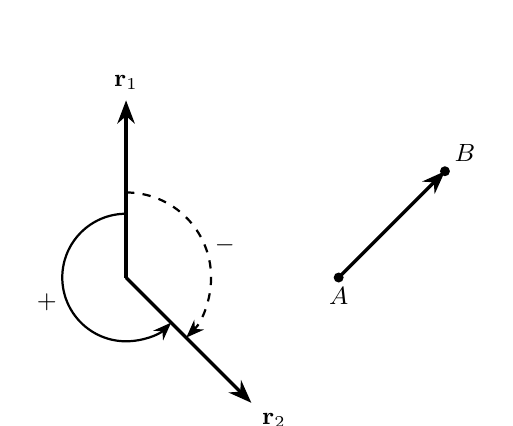
\begin{tikzpicture}[>=Stealth, scale=0.9, font=\small]
  \coordinate (O) at (0, 0);
  \draw[->, very thick] (O) -- (0, 2.5) node[above] {$\mathbf{r}_1$};
  \draw[->, very thick] (O) -- (-45:2.5) node[below right] {$\mathbf{r}_2$};
  \draw[->, thick] (0, 0.9) arc (90:315:0.9) node[midway, left] {$+$};
  \draw[->, thick, dashed] (0, 1.2) arc (90:-45:1.2) node[midway, right] {$-$};
  
  \coordinate (A) at (3, 0);
  \coordinate (B) at (4.5, 1.5);
  \draw[->, very thick] (A) -- (B);
  \fill (A) circle (2pt) node[below] {$A$};
  \fill (B) circle (2pt) node[above right] {$B$};
\end{tikzpicture}
\caption{有向角與有向線段決定條件之差異}
\label{fig:b3-fig2-11}
\end{figure}

\subsubsection*{戊、同界角}

兩個（廣義）有向角，若具有相同的始邊與終邊，則稱它們互為\textbf{同界角}或\textbf{互為同界}. 例如圖 2-8 左圖中，轉 $+60^\circ$ 的角與轉 $+780^\circ$ 的角互為同界，而右圖中，轉 $+210^\circ$ 的角與轉 $-510^\circ$ 的角亦互為同界。

我們注意到兩個有向角 $\angle(\theta; \mathbf{r}_1, \mathbf{r}_2)$ 與 $\angle(\theta'; \mathbf{r}_1', \mathbf{r}_2')$ 互為同界角的一個充分必要條件是
\[ \mathbf{r}_1' = \mathbf{r}_1 \quad\text{且}\quad \theta' = \theta + 360^\circ \text{ 的整倍數} \]
要注意這個整倍數可以為正的倍數也可以為負的倍數。例如圖 2-5 中角度分別為 $+120^\circ$ 與 $-240^\circ$ 的兩個（有向）角具有共同的始邊與終邊，它們是同界的。這例子中
\[ -240^\circ = 120^\circ - 360^\circ \]
所取的倍數是 $-1$。

同樣，兩個無向角，若具有相同的兩個邊，也稱它們互為同界角或互為同界。例如圖 2-5 中的兩個無向角，角度一為 $120^\circ$，一為 $240^\circ$，卻互為同界角。注意這時候，兩個角度的差並不是 $360^\circ$ 的整倍數倒是這兩個角度的和等於 $360^\circ$。這是一般的事實，換句話說，若兩個無向角 $\angle\theta$ 與 $\angle\theta'$ 互為同界角，則
\[ \theta + \theta' = 360^\circ \]

\subsubsection*{己、角度的單位}

以上我們已習慣地利用了 360 度制來作為角度的單位，當我們採用一種單位來度量角時，我們是假定了自己已很清楚什麼時候兩個角叫做大小「相等」。在我們進一步討論各種角度單位之前，先回過頭來解說角的「相等」：

兩個角 $\angle(\theta; \mathbf{r}_1, \mathbf{r}_2)$ 與 $\angle(\theta'; \mathbf{r}_1', \mathbf{r}_2')$ 我們根據什麼來說誰大誰小？

角的大小是根據「疊合」或「全等」的觀念來作為比較的基礎。

\begin{figure}[H]
\centering
\begin{tikzpicture}[>=Stealth, scale=0.88, line cap=round, line join=round, font=\small]
  % 2-12-1
  \coordinate (A1) at (0, 0);
  \draw[->, thick] (A1) -- (-25:2.5) node[below right] {$\mathbf{r}_1$};
  \draw[->, thick] (A1) -- (20:2.5) node[above right] {$\mathbf{r}_2$};
  \draw (-25:0.75) arc (-25:20:0.75) node[midway, right=2pt] {$\theta$};
  \node[left] at (A1) {$A$};
  \node at (1.1, -1.65) {圖 2-12-1};

  % 2-12-2
  \coordinate (A2) at (4.4, -0.35);
  \draw[->, thick] (A2) -- ++(32:2.6) node[right] {$\mathbf{r}_1'$};
  \draw[->, thick] (A2) -- ++(68:2.6) node[above] {$\mathbf{r}_2'$};
  \draw[->, thick, dashed] (A2) -- ++(88:2.6) node[above left] {$\mathbf{r}_2$};
  \draw ($(A2)+(32:0.75)$) arc (32:68:0.75);
  \node at ($(A2)+(50:1.05)$) {\scriptsize $\theta'$};
  \draw[dashed] ($(A2)+(32:1.35)$) arc (32:88:1.35);
  \node[fill=white, inner sep=0.8pt] at ($(A2)+(77:1.55)$) {\scriptsize $\theta$};
  \node[below left] at (A2) {$A'$};
  \node at (5.6, -0.95) {$(\theta > \theta')$};
  \node at (5.6, -1.65) {圖 2-12-2};

  % 2-12-3
  \coordinate (A3) at (9.6, -0.15);
  \draw[->, thick] (A3) -- ++(125:2.4) node[above left] {$\mathbf{r}_1'$};
  \draw[->, thick] (A3) -- ++(38:2.4) node[above right] {$\mathbf{r}_2'$};
  \draw[->, thick, dashed] (A3) -- ++(180:2.2);
  \draw ($(A3)+(125:0.7)$) arc (125:180:0.7);
  \node at ($(A3)+(152:1.05)$) {\scriptsize $\theta$};
  \draw ($(A3)+(125:0.45)$) arc (125:398:0.45);
  \node[right=1pt] at ($(A3)+(-15:0.52)$) {\scriptsize $\theta'$};
  \node[below=5pt] at (A3) {$A'$};
  \node at (10.3, -1.08) {$(\theta < \theta')$};
  \node at (9.7, -1.72) {圖 2-12-3};
\end{tikzpicture}
\end{figure}

亦即：將 $\mathbf{r}_1$ 疊到 $\mathbf{r}_1'$ 上，使起點 $A$ 與 $A'$ 重合，且兩個角皆在 $\mathbf{r}_1$ 的同一側，如果移過去後的 $\mathbf{r}_2$ 已經跨出了 $\theta'$ 的範圍，則稱 $\theta > \theta'$；如還停在 $\theta'$ 的內部，則稱 $\theta < \theta'$；當它與 $\mathbf{r}_2'$ 重疊，則稱 $\theta = \theta'$。

\textbf{(i) 360 度制}

既然根據「疊合」我們能夠比較角的大小，特殊地也使兩個角度相等有了意義，那麼 360 度制也就清楚地有了意義，亦即我們將繞一整圈的角分成 360 個「相等的」角，每一個等分後的角其角度稱為一度，然後每一度又等分成 60 分，每一分再等分成 60 秒，很多角其角度便能記成像 $163^\circ 18' 36''$ 的式樣，其中「${}^\circ$」表度，「$'$」表分，「$''$」表示秒。（當然這樣的角度亦可寫成 $163.31$ 度）。

當然還有很多很多角的角度不能恰巧記為這個樣子，正如有很多實數不能剛好記成一個有限小數一樣。但第二冊中我們採用極限來描述所有的實數；同樣利用極限，則任意一角便可以在 360 度制的意味下數量化，而對應於一個實數。

\textbf{(ii) 弧度制}

其實另一種角度數量化的辦法，更值得採用。考慮單位圓（即半徑為 1 的圓）。任何以圓心 $O$ 為頂點的角，其角度大小，可利用它兩邊所夾之單位圓弧長來度量。

（道理是：根據「疊合」若兩角相等，則這兩角相應的圓弧長亦應相等）。

今取弧長為 1，其相應的角稱為\textbf{一弧度}，即

\begin{figure}[H]
\centering
\begin{minipage}{0.4\textwidth}
\centering
\begin{tikzpicture}[>=Stealth, scale=1.1, font=\small]
  \coordinate (O) at (0, 0);
  \draw[thick] (O) -- (2, 0) node[midway, below] {$1$};
  \draw[thick] (O) -- (57.3:2) node[midway, above left] {$1$};
  \draw[very thick] (2, 0) arc (0:57.3:2) node[midway, right] {$1$};
  \node at (0.5, 0.25) {$\theta$};
  \node[right] at (2.4, 0.8) {——此時 $\theta$ 為一弧度。};
\end{tikzpicture}
\caption{一弧度定義}
\label{fig:b3-fig2-13-2}
\end{minipage}
\hfill
\begin{minipage}{0.55\textwidth}
\centering
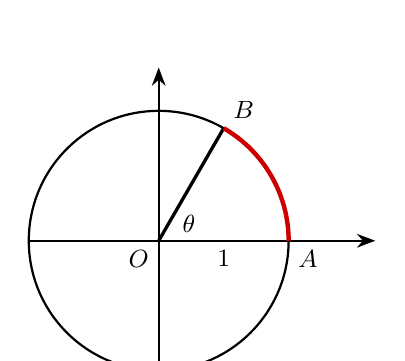
\begin{tikzpicture}[>=Stealth, scale=1.1, font=\small]
  \draw[->, thick] (-1.5, 0) -- (2.5, 0);
  \draw[->, thick] (0, -1.5) -- (0, 2);
  \draw[thick] (0, 0) circle (1.5cm);
  \coordinate (O) at (0, 0);
  \coordinate (A) at (1.5, 0);
  \coordinate (B) at (60:1.5);
  \draw[very thick] (O) -- (B);
  \draw[ultra thick, red!80!black] (A) arc (0:60:1.5);
  \node[below left] at (O) {$O$};
  \node[below right] at (A) {$A$};
  \node[above right] at (B) {$B$};
  \node at (0.35, 0.2) {$\theta$};
  \node[below] at (0.75, 0) {$1$};
\end{tikzpicture}
\caption{單位圓弧長度量角}
\label{fig:b3-fig2-13-1}
\end{minipage}
\end{figure}

單位圓半圓周長是一個無理數，約 $3.14159\dots\dots$，四捨五入後略為 $3.1416$ 通常以符號 $\pi$ 記之；即 $\pi = \text{單位圓半圓周長} = 3.14159\dots\dots \doteq 3.1416$。

考慮兩圓，半徑分別為 1 與 $r$。考慮它們夾在一個角 $\angle\theta$ 內部的圓弧 $\wideparen{AB}$ 與 $\wideparen{A'B'}$，若用弧度制，則 $\wideparen{AB}$ 弧長 $= \theta$，今欲證

\begin{proposition}
以 $r$ 為半徑，對圓心張出圓心角 $\angle\theta$ 的圓弧，弧長為 $r\theta$，亦即
\[ \wideparen{A'B'} \text{ 弧長} = r\theta \]
\end{proposition}

\begin{figure}[H]
\centering
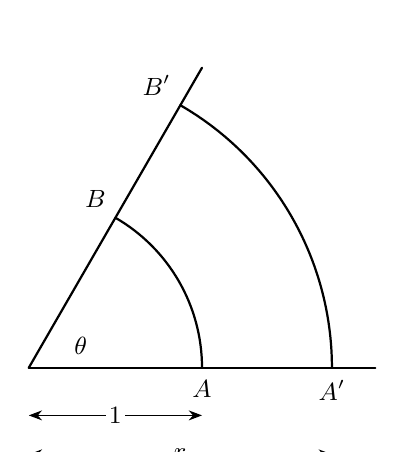
\begin{tikzpicture}[>=Stealth, scale=1.1, line cap=round, line join=round, font=\small]
  \coordinate (O) at (0, 0);
  \draw[thick] (O) -- (4, 0);
  \draw[thick] (O) -- (60:4);
  \draw[thick] (2, 0) arc (0:60:2);
  \draw[thick] (3.5, 0) arc (0:60:3.5);
  \node[below=1pt] at (2, 0) {$A$};
  \node[above left] at (60:2) {$B$};
  \node[below=1pt] at (3.5, 0) {$A'$};
  \node[above left] at (60:3.5) {$B'$};
  \node at (0.6, 0.25) {$\theta$};
  \draw[<->] (0, -0.55) -- (2, -0.55) node[midway, fill=white, inner sep=1pt] {$1$};
  \draw[<->] (0, -1.0) -- (3.5, -1.0) node[midway, fill=white, inner sep=1pt] {$r$};
\end{tikzpicture}
\caption{同心圓弧長與半徑成正比}
\label{fig:b3-fig2-14}
\end{figure}

\begin{proof}
弧長 $\wideparen{AB}$ 與 $\wideparen{A'B'}$ 其實分別是折線 $AC_1 \cup C_1 C_2 \cup \dots \cup C_n B$ 與 $A'C_1' \cup C_1' C_2' \cup \dots \cup C_n' B'$ 當分割 $C_1, C_2, \dots, C_n$ 為無限細密時的極限（見圖 2-15）。

但因 $\overline{OA'} = r\overline{OA}$, $\overline{OC_1'} = r\overline{OC_1}$，得 $\triangle AOC_1 \sim \triangle A'OC_1'$，故 $\overline{A'C_1'} = r\overline{AC_1}$。

同理 $\overline{C_1' C_2'} = r\overline{C_1 C_2}, \dots, \overline{C_n' B'} = r\overline{C_n B}$。

故沿 $\wideparen{A'B'}$ 之折線長
\[ \overline{A'C_1'} + \overline{C_1'C_2'} + \dots + \overline{C_n'B'} \]
為沿 $\wideparen{AB}$ 之折線長
\[ \overline{AC_1} + \overline{C_1 C_2} + \dots + \overline{C_n B} \]
之 $r$ 倍。取分割為無限細密時之極限，得 $\wideparen{A'B'}$ 弧長為 $\wideparen{AB}$ 弧長之 $r$ 倍，亦即
\[ \wideparen{A'B'} \text{ 弧長} = r\wideparen{AB} \text{ 弧長} = r\theta \qedhere \]
\end{proof}

\begin{figure}[H]
\centering
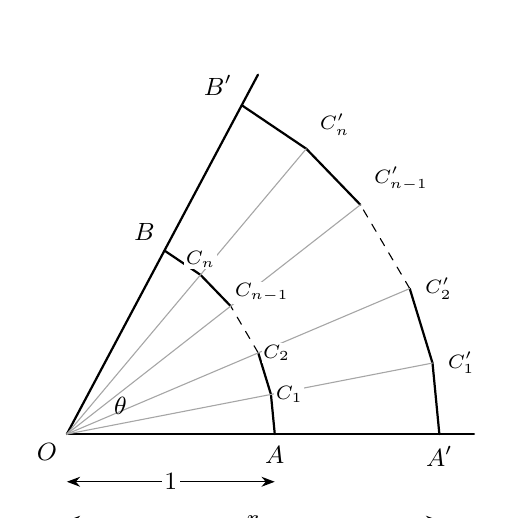
\begin{tikzpicture}[>=Stealth, scale=1.1, line cap=round, line join=round, font=\small]
  \coordinate (O) at (0, 0);
  \draw[thick] (O) -- (4.7, 0);
  \draw[thick] (O) -- (62:4.7);

  % Inner arc & points (well spaced angles)
  \coordinate (A) at (2.4, 0);
  \coordinate (c1) at (11:2.4);
  \coordinate (c2) at (23:2.4);
  \coordinate (cnm1) at (38:2.4);
  \coordinate (cn) at (50:2.4);
  \coordinate (B) at (62:2.4);
  \draw[thick] (A) -- (c1) -- (c2);
  \draw[dashed] (c2) -- (cnm1);
  \draw[thick] (cnm1) -- (cn) -- (B);

  % Outer arc & points
  \coordinate (Aprime) at (4.3, 0);
  \coordinate (c1p) at (11:4.3);
  \coordinate (c2p) at (23:4.3);
  \coordinate (cnm1p) at (38:4.3);
  \coordinate (cnp) at (50:4.3);
  \coordinate (Bprime) at (62:4.3);
  \draw[thick] (Aprime) -- (c1p) -- (c2p);
  \draw[dashed] (c2p) -- (cnm1p);
  \draw[thick] (cnm1p) -- (cnp) -- (Bprime);

  % Radial lines
  \draw[gray!70] (O) -- (c1p);
  \draw[gray!70] (O) -- (c2p);
  \draw[gray!70] (O) -- (cnm1p);
  \draw[gray!70] (O) -- (cnp);

  % Labels (zero collisions)
  \node[below=1pt] at (A) {$A$};
  \node[below=1pt] at (Aprime) {$A'$};
  \node[above left] at (B) {$B$};
  \node[above left] at (Bprime) {$B'$};
  \node[right=1pt, fill=white, inner sep=0.6pt] at (c1) {\scriptsize $C_1$};
  \node[right=2pt] at (c1p) {\scriptsize $C_1'$};
  \node[right=1pt, fill=white, inner sep=0.6pt] at (c2) {\scriptsize $C_2$};
  \node[right=2pt] at (c2p) {\scriptsize $C_2'$};
  \node[above right=1pt, fill=white, inner sep=0.6pt] at (cnm1) {\scriptsize $C_{n-1}$};
  \node[above right=2pt] at (cnm1p) {\scriptsize $C_{n-1}'$};
  \node[above=2pt, fill=white, inner sep=0.6pt] at (cn) {\scriptsize $C_n$};
  \node[above right=2pt] at (cnp) {\scriptsize $C_n'$};
  \node[below left] at (O) {$O$};
  \node at (28:0.7) {$\theta$};

  \draw[<->] (0, -0.55) -- (2.4, -0.55) node[midway, fill=white, inner sep=1pt] {$1$};
  \draw[<->] (0, -1.0) -- (4.3, -1.0) node[midway, fill=white, inner sep=1pt] {$r$};
\end{tikzpicture}
\caption{極限分割與弧長比例}
\label{fig:b3-fig2-15}
\end{figure}

這個命題舉出弧度制的一個好處。以下我們都採用弧度制，必要用 360 度制時會特別聲明。

一周角便是射線正向旋轉一整圈又回到原來位置的角。因單位圓圓周長為 $2\pi$，故周角的角度亦為 $2\pi$。

\begin{corollary}
一個以 $r$ 為半徑的圓，其圓周長為 $2\pi r$。
\end{corollary}

\begin{proof}
當上述命題中之角度 $\theta$ 取為周角 $2\pi$，即得圓周長為 $2\pi r$。
\end{proof}

\textbf{注意}：半周角所對單位圓弧長為單位圓半周長 $\pi$，故為 $\pi$ 弧度，直角所夾的單位圓圓弧長 $\frac{\pi}{2}$，故其在弧度制下之度量為 $\frac{\pi}{2}$ 弧度。

\subsubsection*{作業 1}
採用弧度制，下列角度若干？
\begin{enumerate}[label=\roman*), leftmargin=2.5em]
  \item $\frac{1}{16}$ 周角 \qquad\qquad ii) $\frac{1}{3}$ 周角
  \item[iii)] $\frac{1}{6}$ 周角 \qquad\qquad iv) $\frac{1}{10}$ 周角
\end{enumerate}

\begin{example}
弧度制與 360 度制都是數量化角的度量制度\footnote{此二制的換算表見附錄二表 3.}，其間換算關係可如下求得：

因一半圓所對的圓心角為一平角。等於 $180^\circ$，故有
\[ 180^\circ = \pi \text{ 弧度} \]
所以
\[ 1^\circ = \frac{\pi}{180} \text{ 弧度} \doteq 0.0175 \text{ 弧度} \]
\[ 1 \text{ 弧度} = \left(\frac{180}{\pi}\right)^\circ \doteq (57.296)^\circ = 57^\circ 17' 45'' \qedhere \]
\end{example}

\subsubsection*{作業 2}
給了 360 度制下的角度，試求其弧度
\begin{enumerate}[label=\roman*), leftmargin=2.5em]
  \item $50^\circ$ \qquad\qquad ii) $42^\circ 24' 35''$ \qquad\qquad iii) $135^\circ$ \qquad\qquad iv) $210^\circ$
\end{enumerate}

\subsubsection*{作業 3}
試求下列角度在 360 度制下之度數
\begin{enumerate}[label=\roman*), leftmargin=2.5em]
  \item $\frac{3\pi}{4}$ \qquad\qquad ii) $2$ \qquad\qquad iii) $\frac{\pi}{6}$ \qquad\qquad iv) $\frac{7}{5}$
\end{enumerate}

\subsubsection*{庚、扇形}

既然我們已經提過用折線逼近圓弧，不妨接下去考慮扇形面積及圓面積：

所謂扇形是一個在圓內夾在自圓心出發的兩根射線間的部分，其頂角則為這兩射線所夾的角度，這角度可以是 0 到 $2\pi$ 間的任何角度。如下圖 (2-16) 之扇形常記以 $\sphericalangle OAB$ 或直接寫成 扇形 $OAB$。 $OA$ 或 $OB$ 之長稱為扇形之徑，即 $\overline{OA}$ 或 $\overline{OB}$。

\begin{figure}[H]
\centering
\begin{minipage}{0.48\textwidth}
\centering
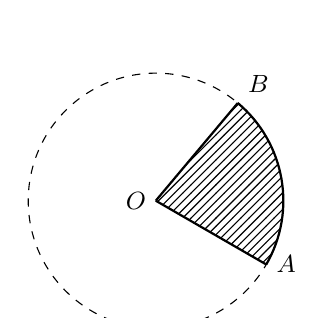
\begin{tikzpicture}[>=Stealth, scale=0.9, font=\small]
  \coordinate (O) at (0, 0);
  \draw[dashed] (O) circle (1.8cm);
  \coordinate (A) at (-30:1.8);
  \coordinate (B) at (50:1.8);
  \draw[thick] (O) -- (A) node[right] {$A$};
  \draw[thick] (O) -- (B) node[above right] {$B$};
  \draw[thick] (A) arc (-30:50:1.8);
  \fill[pattern=north east lines] (O) -- (A) arc (-30:50:1.8) -- cycle;
  \node[left] at (O) {$O$};
\end{tikzpicture}
\end{minipage}
\hfill
\begin{minipage}{0.48\textwidth}
\centering
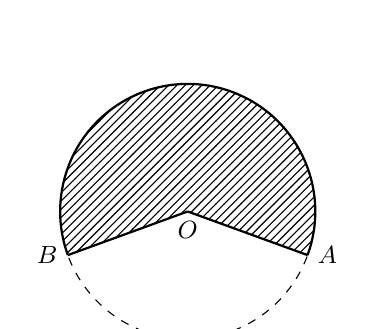
\begin{tikzpicture}[>=Stealth, scale=0.9, font=\small]
  \coordinate (O) at (0, 0);
  \draw[dashed] (O) circle (1.8cm);
  \coordinate (A) at (-20:1.8);
  \coordinate (B) at (200:1.8);
  \draw[thick] (O) -- (A) node[right] {$A$};
  \draw[thick] (O) -- (B) node[left] {$B$};
  \draw[thick] (A) arc (-20:200:1.8);
  \fill[pattern=north east lines] (O) -- (A) arc (-20:200:1.8) -- cycle;
  \node[below] at (O) {$O$};
\end{tikzpicture}
\end{minipage}
\caption{扇形之頂角範圍}
\label{fig:b3-fig2-16}
\end{figure}

\begin{proposition}[扇形面積]
若扇形 $OAB$ 之頂角為 $\theta$，半徑為 $r$，則其面積為 $\frac{1}{2}r^2\theta$。
\end{proposition}

\begin{proof}
設折線 $AC_1 \cup C_1 C_2 \cup \dots \cup C_n B$ 如圖 2-17 逼近 $\wideparen{AB}$，則
\[ \triangle OAC_1,\; \triangle OC_1 C_2,\; \dots,\; \triangle OC_n B \]
面積的和亦逼近扇形 $AOB$ 的面積。

但這些小三角形之高很逼近於 $r$，設其頂角分別為 $\theta_1, \theta_2, \dots, \theta_{n+1}$，則 $\theta = \theta_1 + \theta_2 + \dots + \theta_{n+1}$ 而小三角形底邊長則分別逼近於弧長 $\wideparen{AC_1}, \wideparen{C_1 C_2}, \dots, \wideparen{C_n B}$。亦即分別逼近於 $r\theta_1, r\theta_2, \dots, r\theta_{n+1}$。

故小三角形之面積和逼近於
\[ \frac{1}{2}r(r\theta_1) + \frac{1}{2}r(r\theta_2) + \dots + \frac{1}{2}r(r\theta_{n+1}) = \frac{1}{2}r^2\theta \]
故取了無限細密的分割之極限後，得
\[ \text{扇形 } OAB \text{ 面積} = \frac{1}{2}r^2\theta \qedhere \]
\end{proof}

\begin{figure}[H]
\centering
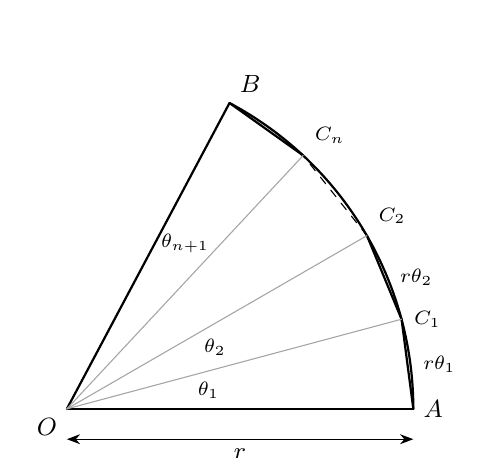
\begin{tikzpicture}[>=Stealth, scale=1.1, line cap=round, line join=round, font=\small]
  \coordinate (O) at (0, 0);
  \draw[thick] (O) -- (4, 0) node[right] {$A$};
  \draw[thick] (O) -- (62:4) node[above right] {$B$};
  \draw[thick] (4, 0) arc (0:62:4);

  % Subdivisions
  \coordinate (c1) at (15:4);
  \coordinate (c2) at (30:4);
  \coordinate (cn) at (47:4);

  \draw[thick] (4, 0) -- (c1) node[midway, right=2pt] {\scriptsize $r\theta_1$};
  \draw[thick] (c1) -- (c2) node[midway, right=2pt] {\scriptsize $r\theta_2$};
  \draw[dashed] (c2) -- (cn);
  \draw[thick] (cn) -- (62:4);

  \draw[gray!70] (O) -- (c1);
  \draw[gray!70] (O) -- (c2);
  \draw[gray!70] (O) -- (cn);

  \node[right=1pt] at (c1) {\scriptsize $C_1$};
  \node[above right=1pt] at (c2) {\scriptsize $C_2$};
  \node[above right=1pt] at (cn) {\scriptsize $C_n$};

  \node at (7.5:1.65) {\scriptsize $\theta_1$};
  \node at (22.5:1.85) {\scriptsize $\theta_2$};
  \node at (54.5:2.35) {\scriptsize $\theta_{n+1}$};
  \node[below left] at (O) {$O$};
  \draw[<->] (0, -0.35) -- (4, -0.35) node[midway, below] {$r$};
\end{tikzpicture}
\caption{扇形面積極限逼近}
\label{fig:b3-fig2-17}
\end{figure}

\begin{corollary}[圓面積]
圓面積為 $\pi r^2$。
\end{corollary}

\begin{proof}
若取頂角 $\theta$ 為周角 $2\pi$ 時，扇形變成圓本身，故圓面積為
\[ \frac{1}{2}r^2\theta = \frac{1}{2}r^2(2\pi) = \pi r^2 \qedhere \]
\end{proof}

\subsubsection*{習題 2-1}

\begin{enumerate}[label=\arabic*., leftmargin=2em]
  \item 設圓的半徑為 2，試求下列各圓心角所對之弧長。
  \begin{enumerate}[label=(\roman*), leftmargin=2.5em]
    \item $30^\circ$ \qquad (ii) $45^\circ$ \qquad (iii) $60^\circ$ \qquad (iv) $120^\circ$
    \item[(v)] $150^\circ$ \qquad (vi) $225^\circ$ \qquad (vii) $270^\circ$
  \end{enumerate}
  \item 試求上題中各圓心角所張扇形之面積。
  \item 設腳踏車輪的直徑為 70 公分，試求旋轉 500 圈所行之距離。
  \begin{flushright}
  \begin{tikzpicture}[>=Stealth, scale=0.85, baseline=(current bounding box.center)]
    \draw[thick] (0, 0) circle (1.5cm);
    \fill (0, 0) circle (2pt) node[left] {太陽};
    \coordinate (E1) at (60:1.5);
    \coordinate (E2) at (85:1.5);
    \draw (0, 0) -- (E1);
    \draw (0, 0) -- (E2);
    \fill[pattern=north east lines] (0, 0) -- (E1) arc (60:85:1.5) -- cycle;
    \fill (E1) circle (2pt) node[right] {地球};
  \end{tikzpicture}
  \end{flushright}
  \item 某甲騎着自行車走了一哩路，車輪直徑為 28 吋，試問車輪轉了幾圈？所轉周角的角度若干？（註：1 哩 = 5280 呎）
  \item 時鐘從八點十分到九點，時針、分針、秒針經過的角度各若干？
  \item 設一正方形之邊長為 $a$，用相鄰二邊為直徑向內各作一圓，求這兩個圓共同部分的面積。
  \item 假設太陽系中的行星以太陽為中心做等速圓周運動，（事實上是以太陽為焦點之橢圓為行進軌道的）地球一年（算它 365 天，或 12 個月）繞一周。太陽與地球的距離已知為 $1.455 \times 10^8$ 公里。試問地球走了一個月或一星期（七天）所相應的轉過的圓心角為若干，所對應的掃過的扇形面積若干？（如圖 2-18）
  \item 
  \begin{enumerate}[label=(\roman*), leftmargin=2.5em]
    \item 將一四邊形分割成兩個三角形，證明四邊形內角和為 $2\pi$。一般地將一個 $n$ 邊形分割成 $(n-2)$ 個三角形，證明 $n$ 邊形內角和為 $(n-2)\pi$。
    \item 考慮一質點沿一個 $n$ 邊形（不拘凹凸）的邊逆時針運動檢驗它方向的變化情形，舉例說明這質點繞一圈回到原來位置時方向正好轉了 $2\pi$。據此再證明 $n$ 邊形的內角和為 $(n-2)\pi$。
  \end{enumerate}
\end{enumerate}

\subsection{三角函數的定義}
\label{subsec:b3-2-2}

國中已講過銳角的三角函數，在那裏我們記得三角函數其實不過是直角三角形各邊的比例。例如正弦、餘弦只是直角邊與斜邊之比，正切、餘切則為兩直角邊之比。

如果將這直角三角形各邊比例預先根據一個內角的大小相當準確地列出一張表，稱為\textbf{三角函數表}，便可拿出去航海，這是十八世紀所謂「書本航海」的開始。在航海史上是個新的紀元。

它的基本精神在於利用相似三角形的原理。只要知道原來地理或天文上圖形的一邊，便可把它縮成紙上作業，利用基本的直觀幾何的原理並參照編好的三角函數表來求得地理或天文圖形上未知的邊長。這樣的過程在國中的三角測量裏，我們已經提及，而在本章第 5 節中，我們將要作進一步的討論。

其實三角函數的好處，不止在於三角測量。自然界的各種波動竟是正弦函數（或餘弦函數）。這現象在電磁學的發展上，一直佔著很重要的地位。這些會在下節的例題中提及。

\subsubsection*{甲、銳角的三角函數}

先複習一下國中提過的，銳角三角函數的定義。

給了一個銳角 $\angle(\theta; \mathbf{r}_1, \mathbf{r}_2)$，銳角意為 $0 < \theta < \frac{\pi}{2}$，設 $A$ 為 $\mathbf{r}_1$ 與 $\mathbf{r}_2$ 的公共起點，在 $\mathbf{r}_1$ 邊上取一點 $C$，在 $C$ 上做 $\mathbf{r}_1$ 的垂線交 $\mathbf{r}_2$ 於 $B$，畫 $\triangle ABC$，如圖 2-19.

\begin{figure}[H]
\centering
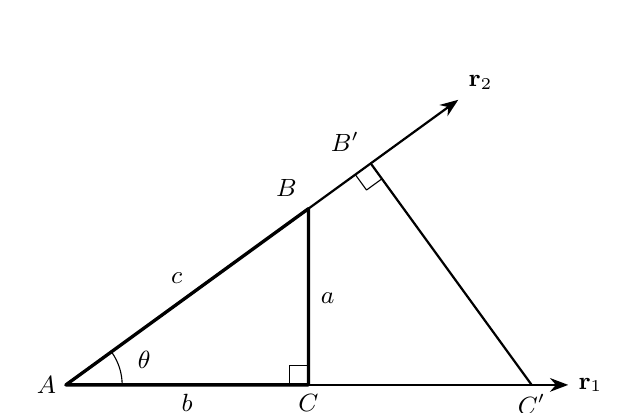
\begin{tikzpicture}[>=Stealth, scale=1.1, line cap=round, line join=round, font=\small]
  \coordinate (A) at (0, 0);
  \coordinate (C) at (2.8, 0);
  \coordinate (B) at (2.8, {2.8*tan(36)});
  % B' on r2, B'C' perpendicular to r2 (matching original scan p. 16 Fig 2-19)
  \coordinate (Bprime) at (36:4.35);
  \coordinate (Cprime) at ({4.35/cos(36)}, 0);

  \draw[->, thick] (A) -- (5.8, 0) node[right] {$\mathbf{r}_1$};
  \draw[->, thick] (A) -- (36:5.6) node[above right] {$\mathbf{r}_2$};

  \draw[very thick] (A) -- (C) -- (B) -- cycle;
  \draw (C) rectangle ++(-0.22, 0.22);

  % Perpendicular B'C' to r2
  \draw[thick] (Bprime) -- (Cprime);
  \draw ($(Bprime)+(-144:0.22)$) -- ++(-54:0.22) -- ($(Bprime)+(-54:0.22)$);

  \node[left] at (A) {$A$};
  \node[below] at (C) {$C$};
  \node[above left=1pt] at (B) {$B$};
  \node[below] at (Cprime) {$C'$};
  \node[above left=1pt] at (Bprime) {$B'$};

  \draw (0.65, 0) arc (0:36:0.65);
  \node at (18:0.95) {$\theta$};
  \node[below] at (1.4, 0) {$b$};
  \node[right=1pt] at (2.8, 1.0) {$a$};
  \node[above left] at (36:1.8) {$c$};
\end{tikzpicture}
\caption{直角三角形與銳角三角函數}
\label{fig:b3-fig2-19}
\end{figure}

設 $\overline{AB} = c$, $\overline{AC} = b$, $\overline{BC} = a$。

則張角 $\angle\theta$ 的六個三角函數值是用直角 $\triangle ABC$ 各邊的兩兩比例來定義的，我們稱 $BC$ 為 $\angle A$ 的對邊，$AC$ 為 $\angle A$ 的鄰邊，$AB$ 為斜邊，它們的長按序記為 $a, b, c$，則規定
\begin{align*}
\sin\theta &= \angle A\text{ 的正弦} = \frac{\text{對邊}}{\text{斜邊}} = \frac{a}{c} \\
\cos\theta &= \angle A\text{ 的餘弦} = \frac{\text{鄰邊}}{\text{斜邊}} = \frac{b}{c} \\
\tan\theta &= \angle A\text{ 的正切} = \frac{\text{對邊}}{\text{鄰邊}} = \frac{a}{b} \\
\cot\theta &= \angle A\text{ 的餘切} = \frac{\text{鄰邊}}{\text{對邊}} = \frac{b}{a} \\
\sec\theta &= \angle A\text{ 的正割} = \frac{\text{斜邊}}{\text{鄰邊}} = \frac{c}{b} \\
\csc\theta &= \angle A\text{ 的餘割} = \frac{\text{斜邊}}{\text{對邊}} = \frac{c}{a}
\end{align*}

雖然以上的定義是依據特定的 $\triangle ABC$ 做出的，要注意的是，所取的邊的比值與所取的直角三角形無關。理由是：$C$ 是 $\mathbf{r}_1$ 上任取的點，取定後，以之為垂足所做的直角三角形均相似，因此邊的比值總是相等的。而另一方面，若不在 $\mathbf{r}_1$ 上取點而改在 $\mathbf{r}_2$ 上取點 $B'$，並以之為垂足做 $\triangle AB'C'$，則由圖易知以 $\triangle AB'C'$ 的邊的比值來定義三角函數結果是相同的，此時 $\overline{B'C'}$ 為 $\angle A$ 的對邊，$\overline{AB'}$ 為 $\angle A$ 的鄰邊，$\overline{AC'}$ 為斜邊。

由以上討論可知：給了一個銳角 $\angle\theta$，所對應的六個數值（比值）只與其角度 $\theta$ 有關，$\theta$ 變時，數值隨之而變，此六數值為相應於 $\theta$ 的應變量，故為 $\theta$ 的函數。又因其函數值與三角形有關，故稱為\textbf{三角函數}，依次記為：
\begin{align*}
\sin\theta &= \theta\text{ 的正弦函數} \\
\cos\theta &= \theta\text{ 的餘弦函數} \\
\tan\theta &= \theta\text{ 的正切函數} \\
\cot\theta &= \theta\text{ 的餘切函數} \\
\sec\theta &= \theta\text{ 的正割函數} \\
\csc\theta &= \theta\text{ 的餘割函數}
\end{align*}

\begin{example}
試比較 $\sin 55^\circ$ 與 $\cos 55^\circ$ 的大小。
\end{example}

\begin{proof}[解]
做 $\triangle ABC$ 使 $\angle A = 55^\circ$, $\angle B = \text{直角}$，則 $\angle C = 90^\circ - 55^\circ = 35^\circ$，而 $\angle A > \angle C$。

三角形內大角對大邊，故有 $\overline{AB} < \overline{BC}$，所以
\[ \sin 55^\circ = \frac{\overline{BC}}{\overline{AC}} > \frac{\overline{AB}}{\overline{AC}} = \cos 55^\circ \qedhere \]
\end{proof}

\begin{figure}[H]
\centering
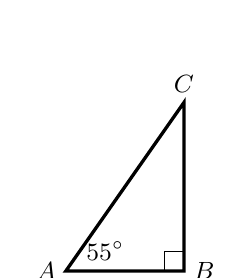
\begin{tikzpicture}[>=Stealth, scale=1.0, font=\small]
  \coordinate (A) at (0, 0);
  \coordinate (B) at (1.5, 0);
  \coordinate (C) at (1.5, 2.14);
  \draw[very thick] (A) -- (B) -- (C) -- cycle;
  \draw (B) rectangle ++(-0.25, 0.25);
  \node[left] at (A) {$A$};
  \node[right] at (B) {$B$};
  \node[above] at (C) {$C$};
  \node at (0.5, 0.25) {$55^\circ$};
\end{tikzpicture}
\caption{$\triangle ABC$ 之角邊關係}
\label{fig:b3-fig2-20}
\end{figure}

\subsubsection*{作業 4}
試比較下列各組函數值之大小。
\begin{enumerate}[label=\roman*), leftmargin=2.5em]
  \item $\sin 40^\circ,\; \cos 40^\circ$ \qquad ii) $\tan 15^\circ,\; \cot 15^\circ$ \qquad iii) $\sec 55^\circ,\; \csc 55^\circ$
\end{enumerate}

\textbf{注意}\quad 到目前為止，三角函數的定義域（即自變數變化的範圍）為 $0 < \theta < \frac{\pi}{2}$。

\begin{example}
試求銳角 $\frac{\pi}{4}$ 之正弦、餘弦與正切。
\end{example}

\begin{proof}[解]
繪 $\triangle ABC$ 使得 $\angle A = \frac{\pi}{4}$，$\angle C = \text{直角}$，則 $\triangle ABC$ 為等腰，$\overline{AC} = \overline{BC}$。

由畢氏定理 $\overline{AC}^2 + \overline{BC}^2 = \overline{AB}^2$，得 $\overline{AB} = \sqrt{2}\;\overline{AC}$。

所以
\begin{align*}
\sin\frac{\pi}{4} &= \sin A = \frac{\overline{BC}}{\overline{AB}} = \frac{1}{\sqrt{2}} \\
\cos\frac{\pi}{4} &= \cos A = \frac{\overline{AC}}{\overline{AB}} = \frac{1}{\sqrt{2}} \\
\tan\frac{\pi}{4} &= \tan A = \frac{\overline{BC}}{\overline{AC}} = 1 \qedhere
\end{align*}
\end{proof}

\begin{figure}[H]
\centering
\begin{minipage}{0.48\textwidth}
\centering
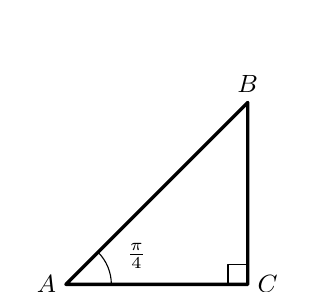
\begin{tikzpicture}[>=Stealth, scale=1.05, line cap=round, line join=round, font=\small]
  \coordinate (A) at (0, 0);
  \coordinate (C) at (2.2, 0);
  \coordinate (B) at (2.2, 2.2);
  \draw[very thick] (A) -- (C) -- (B) -- cycle;
  \draw (C) rectangle ++(-0.24, 0.24);
  \node[left] at (A) {$A$};
  \node[right] at (C) {$C$};
  \node[above] at (B) {$B$};
  \draw (0.55, 0) arc (0:45:0.55);
  \node at (22:0.92) {$\frac{\pi}{4}$};
\end{tikzpicture}
\caption{等腰直角三角形}
\label{fig:b3-fig2-21}
\end{minipage}
\hfill
\begin{minipage}{0.48\textwidth}
\centering
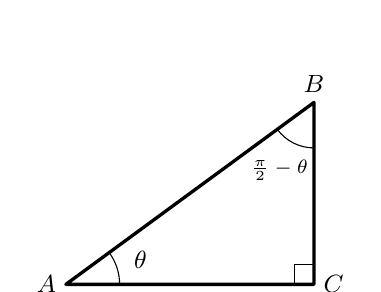
\begin{tikzpicture}[>=Stealth, scale=1.05, line cap=round, line join=round, font=\small]
  \coordinate (A) at (0, 0);
  \coordinate (C) at (3.0, 0);
  \coordinate (B) at (3.0, 2.2);
  \draw[very thick] (A) -- (C) -- (B) -- cycle;
  \draw (C) rectangle ++(-0.24, 0.24);
  \node[left] at (A) {$A$};
  \node[right] at (C) {$C$};
  \node[above] at (B) {$B$};
  \draw (0.65, 0) arc (0:36.25:0.65);
  \node at (18:0.95) {$\theta$};
  \draw ($(B)+(0, -0.55)$) arc (-90:-143.75:0.55);
  \node[fill=white, inner sep=0.5pt] at ($(B)+(-117:0.92)$) {\scriptsize $\frac{\pi}{2}-\theta$};
\end{tikzpicture}
\caption{餘角幾何關係}
\label{fig:b3-fig2-22}
\end{minipage}
\end{figure}

\subsubsection*{作業 5}
試求銳角 $\frac{\pi}{3}$ 與 $\frac{\pi}{6}$ 之三角函數，然後將 $\frac{\pi}{6}, \frac{\pi}{4}, \frac{\pi}{3}$ 各角的三角函數值列表整理。

一個銳角的角度若為 $\theta$，則其餘角為 $\frac{\pi}{2}-\theta$，由銳角三角函數的定義，及圖 2-21 可得：
\begin{align*}
\sin\left(\frac{\pi}{2}-\theta\right) &= \frac{\overline{AC}}{\overline{AB}} = \cos\theta \\
\cos\left(\frac{\pi}{2}-\theta\right) &= \frac{\overline{BC}}{\overline{AB}} = \sin\theta \\
\tan\left(\frac{\pi}{2}-\theta\right) &= \frac{\overline{AC}}{\overline{BC}} = \cot\theta
\end{align*}

此即：一個銳角之餘角的正弦即為此銳角之餘弦，而其餘角之餘弦為此角的正弦。同樣的關係也存在於正切與餘切，正割與餘割之間。總結上述，我們有

\begin{proposition}[銳角的餘角公式]
\begin{align*}
\sin\left(\frac{\pi}{2}-\theta\right) &= \cos\theta,\quad \tan\left(\frac{\pi}{2}-\theta\right) = \cot\theta \\
\sec\left(\frac{\pi}{2}-\theta\right) &= \csc\theta
\end{align*}
\end{proposition}

\begin{example}
設 $\theta_1 < \theta_2$ 為二銳角，試分別比較此二銳角之正弦與餘弦。
\end{example}

\begin{proof}[解]
以 $\mathbf{r}_1$ 為始邊做張角 $\theta_1$ 與 $\theta_2$ 各有終邊 $\mathbf{r}_2, \mathbf{r}_3$。設頂點為 $A$。在 $\mathbf{r}_1$ 上取一點 $B$，在 $B$ 上做 $\mathbf{r}_1$ 垂線各交 $\mathbf{r}_2, \mathbf{r}_3$ 於 $C, D$。則因 $\angle ACB$ 亦為銳角，$\angle ACD$ 必為鈍角，而一三角形內最多只有一個鈍角，故在 $\triangle ACD$ 中，$\angle ACD > \angle ADC$。因三角形內大角對大邊故有 $\overline{AD} > \overline{AC}$。

今
\[ \cos\theta_1 = \frac{\overline{AB}}{\overline{AC}},\qquad \cos\theta_2 = \frac{\overline{AB}}{\overline{AD}} \]
故有 $\cos\theta_1 > \cos\theta_2$。

同理 $\cos\left(\frac{\pi}{2}-\theta_1\right) < \cos\left(\frac{\pi}{2}-\theta_2\right)$。

又由命題 3 知 $\sin\theta_1 = \cos\left(\frac{\pi}{2}-\theta_1\right)$，$\sin\theta_2 = \cos\left(\frac{\pi}{2}-\theta_2\right)$，故有 $\sin\theta_1 < \sin\theta_2$。
\end{proof}

\begin{figure}[H]
\centering
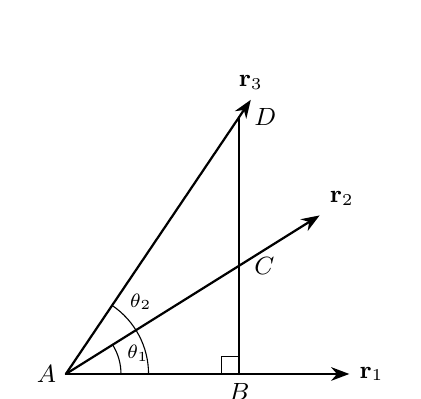
\begin{tikzpicture}[>=Stealth, scale=1.0, line cap=round, line join=round, font=\small]
  \coordinate (A) at (0, 0);
  \draw[->, thick] (A) -- (3.6, 0) node[right] {$\mathbf{r}_1$};
  \draw[->, thick] (A) -- (32:3.8) node[above right] {$\mathbf{r}_2$};
  \draw[->, thick] (A) -- (56:4.2) node[above] {$\mathbf{r}_3$};

  \coordinate (B) at (2.2, 0);
  \coordinate (C) at (2.2, {2.2*tan(32)});
  \coordinate (D) at (2.2, {2.2*tan(56)});

  \draw[thick] (B) -- (D);
  \draw (B) rectangle ++(-0.22, 0.22);

  \node[left] at (A) {$A$};
  \node[below] at (B) {$B$};
  \node[right=2pt] at (C) {$C$};
  \node[right=2pt] at (D) {$D$};

  \draw (0.7, 0) arc (0:32:0.7);
  \node at (16:0.95) {\scriptsize $\theta_1$};
  \draw (1.05, 0) arc (0:56:1.05);
  \node[fill=white, inner sep=0.6pt] at (44:1.32) {\scriptsize $\theta_2$};
\end{tikzpicture}
\caption{銳角單調性幾何證明}
\label{fig:b3-fig2-23}
\end{figure}

\subsubsection*{作業 6}
\begin{enumerate}[label=\roman*), leftmargin=2.5em]
  \item 試比較銳角 $\frac{\pi}{6}, \frac{\pi}{4}, \frac{\pi}{3}$ 之正弦、餘弦與正切。
  \item 試說明在定義域 $0 < \theta < \frac{\pi}{2}$ 內，$\sin\theta$ 與 $\tan\theta$ 為增函數，$\cos\theta$ 為減函數。
\end{enumerate}

由定義，我們可直接得到以下關係式

\begin{proposition}
\begin{align*}
\sin\theta \cdot \csc\theta &= 1 \\
\cos\theta \cdot \sec\theta &= 1 \\
\tan\theta \cdot \cot\theta &= 1
\end{align*}
（即同一角度的正弦與餘割，餘弦與正割，正切與餘切互為倒數）
及
\[ \tan\theta = \frac{\sin\theta}{\cos\theta},\qquad \cot\theta = \frac{\cos\theta}{\sin\theta} \]
\end{proposition}

三角函數表是把 0 度到 45 度的銳角（每 $10'$ 一計，並標出相應的弧度）的三角函數值利用直角三角形邊與邊的比算出，以小數表示橫列出來，所做成的表（附錄），有了這表，便可反過來再利用相似三角形原理計算出：給了一已知邊及已知角的直角三角形的其他邊長。計算時就只要在表中把所需之已知角的某些函數值查出，代入關係式即可。在航海上，天文上，地形測量上都很便利，今只以國中已學過的力的分解來看。

\begin{example}
有一重 $m$ 克的物體放在一坡度 $36^\circ$ 的斜面上，試問此斜面受力多少？
\end{example}

\begin{proof}[解]
物體向地心的重力為 $mg$，$g$ 為重力加速度。此力分解為兩個互相垂直的力：向斜面的壓力 $\vec{OA}$ 及沿斜面下滑的力 $\vec{OB}$。斜面所受壓力與重力 $mg$ 成 $36^\circ$ 角，設此壓力為 $P$ 則
\[ \frac{P}{mg} = \cos 36^\circ \]
\begin{figure}[H]
\centering
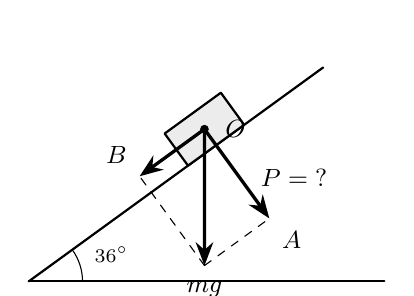
\begin{tikzpicture}[>=Stealth, scale=1.05, line cap=round, line join=round, font=\small]
  % Inclined plane 36 degrees
  \coordinate (O_ground) at (0, 0);
  \draw[thick] (O_ground) -- (4.3, 0);
  \draw[thick] (O_ground) -- (36:4.4);
  \draw (0.65, 0) arc (0:36:0.65);
  \node at (18:1.05) {\scriptsize $36^\circ$};

  % Object on incline
  \coordinate (M) at (36:2.8);
  \begin{scope}[rotate around={36:(M)}]
    \draw[thick, fill=gray!15] ($(M)+(-0.42, 0)$) rectangle ($(M)+(0.42, 0.48)$);
    \coordinate (Center) at ($(M)+(0, 0.24)$);
  \end{scope}

  % Forces from Center
  \coordinate (Fmg) at ($(Center)+(0, -1.65)$);
  \coordinate (FA) at ($(Center)+(-54:1.335)$);
  \coordinate (FB) at ($(Center)+(216:0.97)$);
  \draw[->, very thick] (Center) -- (Fmg) node[below=2pt] {$mg$};
  \draw[->, very thick] (Center) -- (FA) node[below right=1pt] {$A$};
  \node[right=4pt] at ($(Center)!0.55!(FA)$) {$P = {?}$};
  \draw[->, very thick] (Center) -- (FB) node[above left=1pt] {$B$};
  \draw[dashed] (Fmg) -- (FA);
  \draw[dashed] (Fmg) -- (FB);

  \fill (Center) circle (1.5pt);
  \node[above=7pt, right=4pt] at (Center) {$O$};
\end{tikzpicture}
\caption{斜面重力正交分解}
\label{fig:b3-fig2-24}
\end{figure}
查三角函數表知 $\cos 36^\circ = 0.8090$，
\[ \therefore\quad P = mg \cdot \cos 36^\circ = 0.809 mg\text{ 克} \qedhere \]
\end{proof}

\subsubsection*{作業 7}
\begin{enumerate}[label=\roman*), leftmargin=2.5em]
  \item 設有一梯子靠牆放與牆成 $15^\circ$ 角，梯長 6 公尺，問梯頂到牆角距離。
  \item 設一等邊三角形之邊長為 5，試求其高。
  \item 求正六邊形中心到其邊所做垂線之長。
\end{enumerate}

\subsubsection*{乙、三角函數}

現在我們要定義廣義的三角函數。

由於實際的需要，我們把三角函數定義在實數上來代替在角上的定義，以下談到角度我們都固定採用弧度制。

取平面一座標系 $(O; X, Y)$，使 $\vec{OX}$ 到 $\vec{OY}$ 的轉角為 $+\frac{\pi}{2}$（必要時，這樣的座標系稱為正向座標系）。

\begin{definition}
對任一實數 $t$，考慮一廣義有向角 $\angle(\theta; \mathbf{r}_1, \mathbf{r}_2)$，使其始邊 $\mathbf{r}_1 = \vec{OX}$ 且 $\angle\theta$ 的角度 $\theta$ 等於 $t$。在終邊上取一點 $P(x, y)$，使得 $\overline{OP} = 1$。當下列各式右端有意義時（即分母不為 0 時）定義各三角函數如下：
\begin{align*}
\text{正弦}\quad \sin t &= \frac{y}{1} = y \\
\text{餘弦}\quad \cos t &= \frac{x}{1} = x \\
\text{正切}\quad \tan t &= \frac{y}{x} \\
\text{餘切}\quad \cot t &= \frac{x}{y} \\
\text{正割}\quad \sec t &= \frac{1}{x} \\
\text{餘割}\quad \csc t &= \frac{1}{y}
\end{align*}
\end{definition}

\begin{figure}[H]
\centering
\begin{tikzpicture}[>=Stealth, scale=1.1, font=\small]
  \draw[->, thick] (-1.5, 0) -- (2.2, 0) node[right] {$X$};
  \draw[->, thick] (0, -1.5) -- (0, 2) node[above] {$Y$};
  \draw[thick] (0, 0) circle (1.5cm);

  \coordinate (O) at (0, 0);
  \coordinate (P) at (50:1.5);
  \draw[->, very thick] (O) -- (50:2.0) node[above right] {$\mathbf{r}_2$};
  \fill (P) circle (1.5pt) node[right] {$P(x, y)$};
  \draw[dashed] (P) -- ({1.5*cos(50)}, 0) node[below] {$Q$};
  \node[below left] at (O) {$O$};
  \node at (0.35, 0.18) {$\theta$};
  \node[below] at ({0.5*1.5*cos(50)}, 0) {$x$};
  \node[right] at ({1.5*cos(50)}, {0.5*1.5*sin(50)}) {$y$};
  \node[below right] at (1.5, 0) {$(1, 0)$};
  \node[above] at (1.8, 0) {$\mathbf{r}_1$};
  \node[below=1.8cm] at (0.5, 0) {（此圖 $0 < \theta < \frac{\pi}{2};\; x>0, y>0$）};
\end{tikzpicture}
\caption{單位圓廣義三角函數定義 (第一象限)}
\label{fig:b3-fig2-25-1}
\end{figure}

\phantomsection\label{note:b3-ch2-p37-fig2-25-2}%
\begin{figure}[H]
\centering
\begin{minipage}{0.48\textwidth}
\centering
\begin{tikzpicture}[>=Stealth, scale=0.95, line cap=round, line join=round, font=\small]
  \draw[->, thick] (-1.9, 0) -- (1.9, 0) node[right] {$X$};
  \draw[->, thick] (0, -1.6) -- (0, 1.8) node[above] {$Y$};
  \draw[thick] (0, 0) circle (1.3cm);
  \coordinate (O) at (0, 0);
  \coordinate (P) at (135:1.3);
  \draw[->, very thick] (O) -- (135:1.95) node[above left] {$\mathbf{r}_2$};
  \draw[dashed] (P) -- ({1.3*cos(135)}, 0);
  \fill (P) circle (1.5pt) node[above right=2pt, fill=white, inner sep=0.6pt] {\scriptsize $P(x, y)$};
  % Clockwise negative angle matching original scan p. 22 Fig 2-25-2 (-3pi/2 < theta < -pi)
  \draw[->, thick] (0.52, 0) arc (0:-225:0.52);
  \node at (-135:0.8) {$\theta$};
  \node[below] at (1.55, 0) {$\mathbf{r}_1$};
  \node[above right=1pt] at (O) {\scriptsize $O$};
  \node[below=1.65cm] at (0, 0) {\footnotesize （此圖 $-\frac{3\pi}{2} < \theta < \pi$; $x<0, y>0$）\footnotemark};
\end{tikzpicture}
\caption{第二象限角}
\label{fig:b3-fig2-25-2}
\end{minipage}
\hfill
\begin{minipage}{0.48\textwidth}
\centering
\begin{tikzpicture}[>=Stealth, scale=0.95, line cap=round, line join=round, font=\small]
  \draw[->, thick] (-1.7, 0) -- (1.95, 0) node[right] {$X$};
  \draw[->, thick] (0, -1.6) -- (0, 1.8) node[above] {$Y$};
  \draw[thick] (0, 0) circle (1.3cm);
  \coordinate (O) at (0, 0);
  \coordinate (P) at (-40:1.3);
  \draw[->, very thick] (O) -- (-40:1.95) node[below right] {$\mathbf{r}_2$};
  \draw[dashed] (P) -- ({1.3*cos(-40)}, 0);
  \fill (P) circle (1.5pt) node[above right=2pt, fill=white, inner sep=0.6pt] {\scriptsize $P(x, y)$};
  \draw[->, thick, domain=0:680, samples=180, variable=\t]
    plot ({(0.2 + 0.0005*\t)*cos(\t)}, {(0.2 + 0.0005*\t)*sin(\t)});
  \node at (-150:0.85) {$\theta$};
  \node[above] at (1.55, 0) {$\mathbf{r}_1$};
  \node[below left=1pt] at (O) {\scriptsize $O$};
  \node[below=1.65cm] at (0, 0) {\footnotesize （此圖 $\frac{7\pi}{2} < \theta < 4\pi$; $x>0, y<0$）};
\end{tikzpicture}
\caption{多圈旋轉角}
\label{fig:b3-fig2-25-3}
\end{minipage}
\end{figure}
\footnotetext{【校訂註】原書此處排印為「$-\frac{3\pi}{2} < \theta < \pi$」，右端等同正值 $\pi$，而順時針負角旋轉對應第二象限實為 $-\frac{3\pi}{2} < \theta < -\pi$。正文照原刊文字錄入。}

\textbf{注意}
\begin{enumerate}[label=\arabic*., leftmargin=2em]
  \item $\sin t, \cos t$ 的定義域為所有實數，像集為 $[-1, 1]$。
  \item $\tan t, \sec t$ 的定義域為所有 $n\pi + \frac{\pi}{2}$ 以外的實數。其中 $n$ 為任意整數，亦即不為 $\dots\dots -\frac{3\pi}{2}, -\frac{\pi}{2}, \frac{\pi}{2}, \frac{3\pi}{2}\dots\dots$ 之任意實數。
  \item $\cot t, \csc t$ 的定義域為所有 $n\pi$ 以外的實數，其中 $n$ 為任意整數亦即不為 $\dots\dots -2\pi, -\pi, 0, \pi, 2\pi\dots\dots$ 之任意實數。
  \item 雖然這裏我們固定採用弧度制而把三角函數定義在實數上，但有時我們還依習慣，沿用在度數上取值的三角函數，如 $\sin 390^\circ$，它的意義是先將該度數換成弧度，如 $390^\circ = \frac{13\pi}{6}$，而令 $\sin 390^\circ = \sin\frac{13\pi}{6}$。
\end{enumerate}

以下我們分幾段來討論這樣定義下來的三角函數的一些基本性質：

(I) 當 $0 < t < \frac{\pi}{2}$，這個三角函數的定義基本上還是國中提過的銳角的三角函數。如
\begin{align*}
\sin t &= \frac{y}{1} = \frac{b}{c} = \sin\theta \\
\cos t &= \frac{x}{1} = \frac{a}{c} = \cos\theta \quad\text{〔相似形原理〕}
\end{align*}

\begin{figure}[H]
\centering
\begin{tikzpicture}[>=Stealth, scale=1.0, line cap=round, line join=round, font=\small]
  \draw[->, thick] (-0.5, 0) -- (3.6, 0) node[right] {$X$};
  \draw[->, thick] (0, -0.5) -- (0, 2.5) node[above] {$Y$};
  \draw[thick] (1.6, 0) arc (0:90:1.6);
  \coordinate (O) at (0, 0);
  \coordinate (P) at (38:1.6);
  \coordinate (BigP) at (38:3.1);
  \draw[thick] (O) -- (BigP);
  \draw[thick] (P) -- ({1.6*cos(38)}, 0);
  \draw[thick] (BigP) -- ({3.1*cos(38)}, 0);
  \node[below left] at (O) {$O$};
  \draw (0.45, 0) arc (0:38:0.45);
  \node at (18:0.72) {\scriptsize $\theta$};
  \node[above left] at (38:0.95) {$1$};
  \node[above left] at (38:2.1) {$c$};
  \node[right=2pt, fill=white, inner sep=0.6pt] at ({1.6*cos(38)}, 0.48) {$y$};
  \node[right=2pt] at ({3.1*cos(38)}, 0.95) {$b$};
  \node[below] at ({0.5*1.6*cos(38)}, 0) {$x$};
  \draw[<->] (0, -0.55) -- ({3.1*cos(38)}, -0.55) node[midway, fill=white, inner sep=1pt] {$a$};
\end{tikzpicture}
\caption{銳角廣義與直角三角形定義一致性}
\label{fig:b3-fig2-26}
\end{figure}

(II) 從定義得知，既然 $\mathbf{r}_1$ 固定在 $OX$ 軸上，三角函數之值只依賴於終邊的位置，與它相應的 $\angle\theta$ 之旋轉經過無關；例如
\begin{align*}
\sin\frac{2\pi}{3} &= \sin\left(-\frac{4\pi}{3}\right) = \sin\left(\frac{2\pi}{3}-2\pi\right) \\
\sin\frac{2\pi}{3} &= \sin\left(\frac{2\pi}{3}+2\pi\right) = \sin\left(\frac{2\pi}{3}+4\pi\right)
\end{align*}

\begin{figure}[H]
\centering
\begin{minipage}{0.48\textwidth}
\centering
\begin{tikzpicture}[>=Stealth, scale=0.95, line cap=round, line join=round, font=\small]
  \draw[->, thick] (-1.6, 0) -- (1.7, 0) node[right] {$X$};
  \draw[->, thick] (0, -1.6) -- (0, 1.7) node[above] {$Y$};
  \coordinate (O) at (0, 0);
  \coordinate (P) at (120:1.4);
  \draw[thick] (O) -- (P) node[above left] {$P(x, y)$};
  \draw[->, thick] (0.45, 0) arc (0:120:0.45);
  \node[above right] at (45:0.5) {\scriptsize $\frac{2\pi}{3}$};
  \draw[->, thick, dashed] (0.68, 0) arc (0:-240:0.68);
  \node[below right, fill=white, inner sep=0.6pt] at (-65:0.75) {\scriptsize $-\frac{4\pi}{3}$};
  \node[below left] at (120:0.85) {\scriptsize $1$};
\end{tikzpicture}
\caption{$\frac{2\pi}{3}$ 與 $-\frac{4\pi}{3}$ 同界}
\label{fig:b3-fig2-27-1}
\end{minipage}
\hfill
\begin{minipage}{0.48\textwidth}
\centering
\begin{tikzpicture}[>=Stealth, scale=0.95, line cap=round, line join=round, font=\small]
  \draw[->, thick] (-1.6, 0) -- (1.7, 0) node[right] {$X$};
  \draw[->, thick] (0, -1.6) -- (0, 1.7) node[above] {$Y$};
  \coordinate (O) at (0, 0);
  \coordinate (P) at (120:1.4);
  \draw[thick] (O) -- (P) node[above left] {$P(x, y)$};
  \draw[->, thick, domain=0:480, samples=160, variable=\t]
    plot ({(0.2 + 0.00075*\t)*cos(\t)}, {(0.2 + 0.00075*\t)*sin(\t)});
  \node[right] at (0.45, 0.72) {\scriptsize $\frac{2\pi}{3}+2\pi = \frac{8\pi}{3}$};
  \node[below left] at (120:0.95) {\scriptsize $1$};
\end{tikzpicture}
\caption{$\frac{2\pi}{3}$ 與 $\frac{8\pi}{3}$ 同界}
\label{fig:b3-fig2-27-2}
\end{minipage}
\end{figure}

其實，對於任何一個三角函數 $T(t)$（$T$ 可為 $\sin, \cos, \tan, \dots\dots$ 中任何一函數）我們都有
\[ T(t) = T(t + 2n\pi);\qquad n \text{ 為任何整數。} \]
道理的關鍵在於三角函數只依賴於終邊的 $P$ 點座標成分 $x$ 與 $y$，故與 $\angle\theta$ 旋轉的經過無關。因此三角函數是週期性的函數。

$X, Y$ 兩軸把座標平面分割為四部分，每一部分稱為一個象限，自逆時針方向數過來按次稱為第一、二、三、四象限。常以羅馬大寫 $\mathrm{I}, \mathrm{II}, \mathrm{III}, \mathrm{IV}$ 表示，如圖 2-28.

現在我們知道三角函數的值只依賴於終邊的位置，以下便根據終邊座落的位置來看各三角函數的正負變化情形：

當 $t$ 從 0 慢慢增加，經 $\frac{\pi}{2}$，$\pi$，$\frac{3\pi}{2}$ 到 $2\pi$ 的過程中，$\sin t$ 相應地也從 0 開始增加到 1 後降落到 0 更降落到 $-1$，然後又開始增加，慢慢回復到 0. 等 $t$ 超過 $2\pi$ 後，則 $\sin t$ 又重複原來的現象。這樣週而復始地起伏。

列表將各函數的正負變化描出，也許清楚一些。（但這表也不是用來強記的）

\begin{figure}[H]
\centering
\begin{tikzpicture}[>=Stealth, scale=1.0, line cap=round, line join=round, font=\small]
  \draw[->, thick] (-2.1, 0) node[left] {$X'$} -- (2.2, 0) node[right] {$X$};
  \draw[->, thick] (0, -2.1) node[below] {$Y'$} -- (0, 2.2) node[above] {$Y$};
  \draw[thick] (0, 0) circle (1.35cm);
  \node at (1.55, 1.35) {$\mathrm{I}$};
  \node at (-1.68, 0.72) {$\mathrm{II}$};
  \node at (-1.55, -1.35) {$\mathrm{III}$};
  \node at (1.55, -1.35) {$\mathrm{IV}$};
  \coordinate (O) at (0, 0);
  \coordinate (P) at (138:1.35);
  \draw[->, thick] (O) -- (138:2.1) node[above left] {$\mathbf{r}_2$};
  \fill (P) circle (1.5pt) node[above right=2pt, fill=white, inner sep=0.6pt] {\scriptsize $P(x, y)$};
  \draw[->, thin] (0.4, 0) arc (0:138:0.4);
  \node[fill=white, inner sep=0.5pt] at (55:0.62) {\scriptsize $\theta$};
  \node[below left] at (138:0.68) {\scriptsize $1$};
  \node[below] at (1.75, 0) {$\mathbf{r}_1$};
  \node[below left] at (O) {$O$};
\end{tikzpicture}
\caption{平面之四個象限}
\label{fig:b3-fig2-28}
\end{figure}

\begin{table}[H]
\centering
\footnotesize
\setlength{\tabcolsep}{3pt}
\renewcommand{\arraystretch}{1.25}
\resizebox{\textwidth}{!}{%
\begin{tabular}{|c|c|c|c|c|c|c|c|c|}
\hline
終邊 $\mathbf{r}_2$ 的位置 & $\mathbf{r}_2 = \vec{OX}$ & $\mathbf{r}_2 \subset \mathrm{I}^*$ & $\mathbf{r}_2 = \vec{OY}$ & $\mathbf{r}_2 \subset \mathrm{II}^*$ & $\mathbf{r}_2 = \vec{OX'}$ & $\mathbf{r}_2 \subset \mathrm{III}^*$ & $\mathbf{r}_2 = \vec{OY'}$ & $\mathbf{r}_2 \subset \mathrm{IV}^*$ \\ \hline
\shortstack{$\mathbf{r}_2$ 上 $P$ 點的座\\標 $x$ 與 $y$} & \shortstack{$x=1$\\$y=0$} & \shortstack{$x>0$\\$y>0$} & \shortstack{$x=0$\\$y=1$} & \shortstack{$x<0$\\$y>0$} & \shortstack{$x=-1$\\$y=0$} & \shortstack{$x<0$\\$y<0$} & \shortstack{$x=0$\\$y=-1$} & \shortstack{$x>0$\\$y<0$} \\ \hline
$\sin t = y$ & $0$ & $\stackrel{+}{\nearrow}$ & $1$ & $\stackrel{+}{\searrow}$ & $0$ & $\stackrel{-}{\searrow}$ & $-1$ & $\stackrel{-}{\nearrow}$ \\ \hline
$\cos t = x$ & $1$ & $\stackrel{+}{\searrow}$ & $0$ & $\stackrel{-}{\searrow}$ & $-1$ & $\stackrel{-}{\nearrow}$ & $0$ & $\stackrel{+}{\nearrow}$ \\ \hline
$\tan t = \frac{y}{x}$ & $0$ & $\stackrel{+}{\nearrow}$ & $+\infty \mid -\infty$ & $\stackrel{-}{\nearrow}$ & $0$ & $\stackrel{+}{\nearrow}$ & $+\infty \mid -\infty$ & $\stackrel{-}{\nearrow}$ \\ \hline
$\cot t = \frac{x}{y}$ & $-\infty \mid +\infty$ & $\stackrel{+}{\searrow}$ & $0$ & $\stackrel{-}{\searrow}$ & $-\infty \mid +\infty$ & $\stackrel{+}{\searrow}$ & $0$ & $\stackrel{-}{\searrow}$ \\ \hline
$\sec t = \frac{1}{x}$ & $1$ & $\stackrel{+}{\nearrow}$ & $+\infty \mid -\infty$ & $\stackrel{-}{\nearrow}$ & $-1$ & $\stackrel{-}{\searrow}$ & $-\infty \mid +\infty$ & $\stackrel{+}{\searrow}$ \\ \hline
$\csc t = \frac{1}{y}$ & $-\infty \mid +\infty$ & $\stackrel{+}{\searrow}$ & $1$ & $\stackrel{+}{\searrow}$ & $+\infty \mid -\infty$ & $\stackrel{-}{\nearrow}$ & $-1$ & $\stackrel{-}{\searrow}$ \\ \hline
\end{tabular}%
}
\par\vspace{3pt}
{\footnotesize (* 這裡 $\mathbf{r}_2 \subset \mathrm{I}$ 意指終邊位置落在第一象限)}
\end{table}

\textbf{註}：此表所用 $\infty$ 可以看成無意義，但其實它有深一層的意思，比如當 $\mathbf{r}_2 = \vec{OY}$ 時，在 $t = \frac{\pi}{2}$ 之點 $\tan t$ 沒有定義，但 $\tan t = \pm\infty$ 的意思是當 $t$ 增大而向 $\pi/2$ 逼近時 $\tan t$ 趨於「正無限大」，另一方面當 $t$ 減小而向 $\pi/2$ 逼近時，$\tan t$ 趨於「負無限大」（參見圖 2-30）。

從廣義三角函數的定義知在 $-\infty < t < \infty$ 之間，亦有 $\sin t$ 與 $\csc t$, $\cos t$ 與 $\sec t$, $\tan t$ 與 $\cot t$ 各對函數值互為倒數，即
\[ \sin t = \frac{1}{\csc t},\qquad \cos t = \frac{1}{\sec t},\qquad \tan t = \frac{1}{\cot t} \]
故只注意前面三個函數 $\sin t, \cos t, \tan t$ 的正負變化，便立即或可得相應的 $\csc t, \sec t, \cot t$ 的正負變化情形。

\begin{figure}[H]
\centering
\begin{tikzpicture}[scale=1.0, font=\small]
  \draw[thick] (-2.4, 0) -- (2.4, 0);
  \draw[thick] (0, -1.65) -- (0, 1.65);
  \node at (1.2, 0.9) {\shortstack{$\mathrm{I}$\\全 $+$}};
  \node at (-1.2, 0.9) {\shortstack{$\mathrm{II}$\\$\sin t = +$\\$\csc t = +$}};
  \node at (-1.2, -0.9) {\shortstack{$\mathrm{III}$\\$\tan t = +$\\$\cot t = +$}};
  \node at (1.2, -0.9) {\shortstack{$\mathrm{IV}$\\$\cos t = +$\\$\sec t = +$}};
\end{tikzpicture}
\caption{各象限三角函數正負符號分佈}
\end{figure}

(III) 一質點 $P(x, y)$ 在單位圓上，自 $(1, 0)$ 點出發，以單位角速度〔即每單位時間走一弧度的等速轉動〕沿逆時針方向運動，則在 $t$ 時刻，$P$ 的位置正好落在張角 $\angle\theta$ 之角度為 $t$ 的地方（為什麼？留作習題）故
\[ \sin t = y \quad\text{與}\quad \cos t = x \]
正好描寫這質點 $P(x, y)$ 分別在 $\vec{OY}$ 軸與在 $\vec{OX}$ 軸上的投影。從表二可以描出 $u = \sin t$ 的函數圖形約略是如下的波形：

\begin{figure}[H]
\centering
\begin{tikzpicture}[>=Stealth, scale=0.95, font=\small]
  \draw[->, thick] (-2, 0) -- (7.5, 0) node[right] {$t$};
  \draw[->, thick] (0, -1.8) -- (0, 2) node[above] {$u$};

  \draw[dashed, gray] (-2, 1) -- (7.2, 1);
  \draw[dashed, gray] (-2, -1) -- (7.2, -1);
  \node[left] at (0, 1) {$1$};
  \node[left] at (0, -1) {$-1$};
  \node[below left] at (0, 0) {$O$};

  \draw[very thick, domain=-1.57:6.8, samples=120] plot (\x, {sin(\x r)});

  \node[below] at (-1.57, 0) {\scriptsize $-\frac{\pi}{2}$};
  \node[below] at (1.57, 0) {\scriptsize $\frac{\pi}{2}$};
  \node[below] at (3.14, 0) {\scriptsize $\pi$};
  \node[below] at (4.71, 0) {\scriptsize $\frac{3\pi}{2}$};
  \node[below] at (6.28, 0) {\scriptsize $2\pi$};
\end{tikzpicture}
\caption{$u = \sin t$ 的函數圖形}
\label{fig:b3-fig2-29}
\end{figure}

至於 $u = \cos t$ 的函數圖形留當習題。

(IV) 參照表二中三角函數的變化情形我們畫出 $u = \tan t$ 與 $u = \sec t$ 的函數圖形（而將 $u = \cot t$ 與 $u = \csc t$ 的圖形留當習題）。

\begin{figure}[H]
\centering
\begin{tikzpicture}[>=Stealth, scale=0.9, font=\small]
  \draw[->, thick] (-3.8, 0) -- (7, 0) node[right] {$t$};
  \draw[->, thick] (0, -3) -- (0, 3) node[above] {$u$};

  % Asymptotes
  \foreach \x in {-1.57, 1.57, 4.71} {
    \draw[dashed, gray] (\x, -2.8) -- (\x, 2.8);
  }

  % Tangent branches
  \draw[very thick, domain=-3.6:-1.7, samples=60] plot (\x, {tan(\x r)});
  \draw[very thick, domain=-1.35:1.35, samples=60] plot (\x, {tan(\x r)});
  \draw[very thick, domain=1.75:4.5, samples=60] plot (\x, {tan(\x r)});
  \draw[very thick, domain=4.9:6.6, samples=60] plot (\x, {tan(\x r)});

  \node[below] at (-3.14, 0) {\scriptsize $-\pi$};
  \node[below] at (-1.57, 0) {\scriptsize $-\frac{\pi}{2}$};
  \node[below left] at (0, 0) {$O$};
  \node[below] at (1.57, 0) {\scriptsize $\frac{\pi}{2}$};
  \node[below] at (3.14, 0) {\scriptsize $\pi$};
  \node[below] at (4.71, 0) {\scriptsize $\frac{3\pi}{2}$};
  \node[below] at (6.28, 0) {\scriptsize $2\pi$};
\end{tikzpicture}
\caption{$u = \tan t$ 的圖形}
\label{fig:b3-fig2-30}
\end{figure}

\begin{figure}[H]
\centering
\begin{tikzpicture}[>=Stealth, scale=0.9, font=\small]
  \draw[->, thick] (-3.8, 0) -- (7, 0) node[right] {$t$};
  \draw[->, thick] (0, -3) -- (0, 3) node[above] {$u$};

  \draw[dashed, gray] (-3.8, 1) -- (6.8, 1);
  \draw[dashed, gray] (-3.8, -1) -- (6.8, -1);

  % Asymptotes
  \foreach \x in {-1.57, 1.57, 4.71} {
    \draw[dashed, gray] (\x, -2.8) -- (\x, 2.8);
  }

  % Secant branches
  \draw[very thick, domain=-1.3:1.3, samples=50] plot (\x, {1/cos(\x r)});
  \draw[very thick, domain=1.85:4.4, samples=50] plot (\x, {1/cos(\x r)});
  \draw[very thick, domain=4.95:6.8, samples=50] plot (\x, {1/cos(\x r)});

  \node[below] at (-3.14, 0) {\scriptsize $-\pi$};
  \node[below] at (-1.57, 0) {\scriptsize $-\frac{\pi}{2}$};
  \node[below left] at (0, 0) {$O$};
  \node[below] at (1.57, 0) {\scriptsize $\frac{\pi}{2}$};
  \node[below] at (3.14, 0) {\scriptsize $\pi$};
  \node[below] at (4.71, 0) {\scriptsize $\frac{3\pi}{2}$};
  \node[below] at (6.28, 0) {\scriptsize $2\pi$};
\end{tikzpicture}
\caption{$u = \sec t$ 的圖形}
\label{fig:b3-fig2-31}
\end{figure}

\phantomsection\label{note:b3-ch2-p41-ex4-typo}%
\begin{example}
已知 $\alpha = 1230^\circ$，求 $\sin\alpha, \cos\alpha, \tan\alpha$\footnote{【校訂註】原書題幹印作「$\text{tara }\alpha$」，係「$\tan\alpha$」之印刷訛字，茲校訂為 $\tan\alpha$。} 之值。
\end{example}

\begin{proof}[解]
$1230^\circ = 3 \times 360^\circ + 150^\circ = 3 \times 2\pi + \frac{5\pi}{6}$（弧度）

\phantomsection\label{note:b3-ch2-p41-ref-fig31}%
依定義取 $\angle(\theta; \mathbf{r}_1, \mathbf{r}_2)$ 使 $\mathbf{r}_1$ 與 $OX$ 軸重疊，則終邊 $\mathbf{r}_2$ 落在第二象限 $\mathrm{II}$（如圖 2-31\footnote{【校訂註】原書行文稱「如圖 2-31」，圖 2-31 實為前文割線函數圖形，本例題之旋轉角終邊示意圖印於次頁圖 2-32。正文保留原書字樣。}）

\begin{enumerate}[label=(\roman*), leftmargin=2.5em]
  \item $\sin 1230^\circ = \sin\left(3\times 2\pi + \frac{5\pi}{6}\right) = \sin\frac{5\pi}{6} = y = \frac{1}{2}$
  \item $\cos 1230^\circ = \cos\left(3\times 2\pi + \frac{5\pi}{6}\right) = \cos\frac{5\pi}{6} = x = -\frac{\sqrt{3}}{2}$
  \item $\tan 1230^\circ = \tan\left(3\times 2\pi + \frac{5\pi}{6}\right) = \tan\frac{5\pi}{6} = \frac{y}{x} = -\frac{1}{\sqrt{3}} \qedhere$
\end{enumerate}
\end{proof}

\begin{figure}[H]
\centering
\begin{tikzpicture}[>=Stealth, scale=1.05, line cap=round, line join=round, font=\small]
  \draw[->, thick] (-2.5, 0) -- (2.5, 0) node[right] {$\mathbf{r}_1$};
  \draw[->, thick] (0, -2.2) -- (0, 2.2);
  \draw[thick] (0, 0) circle (1.75cm);
  \coordinate (O) at (0, 0);
  \coordinate (P) at (150:1.75);
  \coordinate (Q) at ({1.75*cos(150)}, 0);
  \draw[->, very thick] (O) -- (150:2.4) node[above left] {$\mathbf{r}_2$};
  \fill (P) circle (1.6pt) node[above=2pt] {$P$};
  \draw[thick] (P) -- (Q) node[below=2pt] {$Q$};
  \draw[->, thick, domain=0:1230, samples=260, variable=\t]
    plot ({(0.16 + 0.00042*\t)*cos(\t)}, {(0.16 + 0.00042*\t)*sin(\t)});
  \node[below right=4pt, fill=white, inner sep=1pt] at (0.45, -0.45) {\scriptsize $O$};
  \node[below=2pt] at (-1.1, 0) {$x$};
  \node[left=2pt] at ({1.75*cos(150)}, 0.48) {$y$};
\end{tikzpicture}
\caption{$1230^\circ$ 旋轉角終邊分析}
\label{fig:b3-fig2-32}
\end{figure}

\begin{example}
若 $\cot t \cos t > 0$，則相應的 $\angle\theta$ 之終邊 $\mathbf{r}_2$ 應落在第幾象限？
\end{example}

\begin{proof}[解]
$\cot t \cos t > 0 \iff \cot t > 0, \cos t > 0$ 或 $\cot t < 0, \cos t < 0$。

故 $\mathbf{r}_2$ 落在第一或第二象限。\qedhere
\end{proof}

\subsubsection*{作業 8}
\begin{enumerate}[label=\roman*), leftmargin=2.5em]
  \item 求下列各三角函數值：
  \[ \cot 150^\circ,\quad \sin 225^\circ,\quad \tan(-570^\circ),\quad \cos\frac{20}{3}\pi \]
  \item 若 $\cos t < 0, \tan t > 0$，則相應的 $\angle\theta$ 之終邊 $\mathbf{r}_2$ 應落在第幾象限？
  \item 點 $(\cot(-4), \sec(-4))$ 應落在第幾象限？
\end{enumerate}

\subsubsection*{習題 2-2}

\begin{enumerate}[label=\arabic*., leftmargin=2em]
  \item 設一質點 $P(x, y)$ 在單位圓上，自 $(1, 0)$ 出發，以角速度 $w=1$（弧度/秒）沿逆時針方向運動，試證在 $t$ 秒時，$P$ 的位置正好落在張角 $\angle\theta$ 之角度為 $t$ 的地方。
  \item 描出 $u = \cos t$ 的圖形。
  \item 描出 $u = \cot t$ 與 $u = \csc t$ 的圖形。
  \item 試求函數曲線 $u = \sin t$ 與 $u = \cos t$ 的交點。
  \item 利用 $t \to 3t \to 3t-\frac{\pi}{2} \to \sin(3t-\frac{\pi}{2}) \to 2\sin(3t-\frac{\pi}{2})$ 這一系列函數的合成函數描出 $u = 2\sin(3t-\frac{\pi}{2})$ 之函數圖形。
  \item 試描出 $u = \sin t + \cos t$ 之函數圖形。
  \item 利用三角函數寫出單位圓內接正六邊形的周長及面積。
  \item[\textbf{*8.}] 圖示下列各式：
  \begin{enumerate}[label=(\roman*), leftmargin=2.5em]
    \item $y = |\sin t|$ \qquad (ii) $y = \cos t - |\cos t|$ \qquad (iii) $y = \csc t + |\csc t|$
  \end{enumerate}
  \stepcounter{enumi}
  \item 已知 $0 < \theta < \frac{\pi}{2}$ 則 $\sin\theta < \theta$ 試證之。（見圖 2-33）
  \begin{flushright}
  \begin{tikzpicture}[>=Stealth, scale=0.85, line cap=round, line join=round, font=\small, baseline=(current bounding box.center)]
    \draw[->, thick] (-1.8, 0) -- (2.1, 0);
    \draw[->, thick] (0, -1.7) -- (0, 1.9);
    \draw[thick] (0, 0) circle (1.35cm);
    \coordinate (O) at (0, 0);
    \coordinate (R) at (1.35, 0);
    \coordinate (P) at (40:1.35);
    \coordinate (Q) at ({1.35*cos(40)}, 0);
    \draw[thick] (O) -- (P) node[above right] {$P$};
    \draw[thick] (P) -- (Q);
    \node[below left] at (O) {$O$};
    \node[below] at (Q) {$Q$};
    \node[below right] at (R) {$R$};
    \node[above left] at (40:0.75) {\scriptsize $1$};
    \node at (19:0.65) {\scriptsize $\theta$};
    \node[below=1.85cm] at (0, 0) {\footnotesize 圖 2-33};
  \end{tikzpicture}
  \end{flushright}
  \item 圖 2-34 中，點 $P$ 之座標為何？
  \begin{flushright}
  \begin{tikzpicture}[>=Stealth, scale=0.9, line cap=round, line join=round, font=\small, baseline=(current bounding box.center)]
    \draw[->, thick] (-1.8, 0) -- (2.2, 0) node[right] {$X$};
    \draw[->, thick] (0, -1.8) -- (0, 1.8) node[above] {$Y$};
    \coordinate (O) at (0, 0);
    \coordinate (P) at (222:1.9);
    \draw[thick] (O) -- (P) node[below left] {$P$};
    \fill (P) circle (1.5pt);
    \draw[->, thick] (0.5, 0) arc (0:222:0.5);
    \node at (48:0.78) {$\theta$};
    \node[below right=1pt] at (222:1.05) {$a$};
    \node[below=1.9cm] at (0, 0) {\footnotesize 圖 2-34};
  \end{tikzpicture}
  \end{flushright}
  \item 假設我們已經知道
  \begin{enumerate}[label=(\roman*), leftmargin=2.5em]
    \item $-1 \le \sin x \le 1$
    \item 當 $x > 0$，滿足 $\sin x = 0$ 之點為 $\pi, 2\pi, 3\pi, \dots\dots$，（稱為 $\sin x$ 之零點）\\
    滿足 $\sin x = +1$ 之點為 $\frac{\pi}{2}, 2\pi+\frac{\pi}{2}, 4\pi+\frac{\pi}{2}, \dots\dots$（稱為 $\sin x$ 之峯點）\\
    滿足 $\sin x = -1$ 之點為 $\frac{3\pi}{2}, 2\pi+\frac{3\pi}{2}, 4\pi+\frac{3\pi}{2}, \dots\dots$（稱為 $\sin x$ 之谷點）
  \end{enumerate}
  我們便概略繪得 $\sin x$ 之函數圖形如下：
  \begin{center}
  \begin{tikzpicture}[>=Stealth, scale=0.85, font=\scriptsize]
    \draw[->, thick] (-0.5, 0) -- (9.5, 0) node[right] {$X$};
    \draw[->, thick] (0, -1.5) -- (0, 1.5) node[above] {$Y$};
    \draw[domain=0:9.42, samples=120, very thick] plot (\x, {sin(\x r)});
    \node[below left] at (0, 0) {$0$};
    \node[below] at (1.57, 0) {$\frac{\pi}{2}$};
    \node[below] at (3.14, 0) {$\pi$};
    \node[below] at (4.71, 0) {$\frac{3\pi}{2}$};
    \node[below] at (6.28, 0) {$2\pi$};
    \node[below] at (7.85, 0) {$2\pi+\frac{\pi}{2}$};
    \node[below] at (9.42, 0) {$3\pi$};
  \end{tikzpicture}
  \end{center}
  \begin{enumerate}[label=(\alph*), leftmargin=2.5em]
    \item 證明：$x \ne 0$; $-1 \le \sin\frac{1}{x} \le 1$
    \item 求 $\sin\frac{1}{x}$ 的零點，峯點、谷點。
    \item 並仿上述大略畫出 $\sin\frac{1}{x}$ 的圖形。
  \end{enumerate}
\end{enumerate}

\subsection{一些簡易的恒等式}
\label{subsec:b3-2-3}

本節將沿用 §2-2 的所有符號。

三角函數之間有各種關係，本節只提一些簡易的恆等式，以供本冊之用，其餘目前用不著的〔像和角公式：即將 $\sin(t_1 + t_2)$ 表成 $t_1$ 與 $t_2$ 的三角函數，如 $\sin t_1, \cos t_2$ 等的公式〕暫時放在一邊，因為它們的一般導引方法是利用圖解，依賴圖解，不僅先天上難具一般性〔如導引和角公式時，要取 $t_1, t_2$ 使相應角度 $\overline{\theta_1}, \overline{\theta_2}$ 落到那一象限呢？〕，而導引的過程也難以表現它的要點。我們這樣做更重要的原因是：我們現在講述三角函數，只為它一些簡易性質將在本冊各種問題的處理需用，中心並不放在三角函數本身。我們希望能很快地能跳過這段三角函數的講述，在作過測量的應用後，迅速轉入本冊的主題：向量幾何與座標幾何的代數轉化！不願現在就陷入三角函數傳統技巧的故紙堆裏。到了第三章，在向量內積引進來後還要利用它導引和角公式。我們無意要把三角函數作為一個獨立的題材來講述。相反地，我們要隨著幾何與代數間的轉化這一主題的需要，和可用來簡捷處理三角函數的各項工具（如向量、複數）的逐次發展，來一步步引出三角函數的各項有用的性質。

\begin{proposition}
對下列函數有定義的任意實數 $t$，我們有下列恆等式
\begin{align*}
\sin^2 t + \cos^2 t &= 1,\qquad 1 + \tan^2 t = \sec^2 t \\
1 + \cot^2 t &= \csc^2 t
\end{align*}
\end{proposition}

\begin{proof}
其實這組恆等式就是畢氏定理的化身：
\[ \sin^2 t + \cos^2 t = y^2 + x^2 = \overline{OP}^2 = 1 \quad\text{〔符號沿用 §2-2 的定義〕} \]
\[ 1 + \tan^2 t = 1 + \frac{y^2}{x^2} = \frac{x^2 + y^2}{x^2} = \frac{1}{x^2} = \sec^2 t \]
\[ 1 + \cot^2 t = 1 + \frac{x^2}{y^2} = \frac{y^2 + x^2}{y^2} = \frac{1}{y^2} = \csc^2 t \qedhere \]
\end{proof}

\begin{proposition}[負角公式]
我們有
\begin{align*}
\sin t &= -\sin(-t) \\
\cos t &= \cos(-t) \\
\tan t &= -\tan(-t)
\end{align*}
\end{proposition}

\begin{proof}
由三角函數的定義知其符號（值）只與其所對應的廣義有向角的終邊的位置有關。今對實數 $t$，取其對應角的始邊為 $OX$，若終邊在第 $\mathrm{I}$ 象限，則對應於 $-t$ 的角的終邊會落在第 $\mathrm{IV}$ 象限，而若終邊在第 $\mathrm{II}$ 象限，則對應於 $-t$ 的角的終邊在第 $\mathrm{III}$ 象限，調換 $\mathrm{I}$ 與 $\mathrm{IV}$ 或 $\mathrm{II}$ 與 $\mathrm{III}$ 的位置結果亦同。今若各在其終邊上取點 $P(x, y), Q(x', y')$，則有 $x = x', y = -y'$（為什麼，請自證）。

今
\begin{align*}
\sin t &= y,\quad \sin(-t) = y' \\
\cos t &= x,\quad \cos(-t) = x' \\
\tan t &= y/x,\quad \tan(-t) = y'/x'
\end{align*}
故得證。
\end{proof}

在 §2-28 甲的作業裏，我們已要同學們算幾個特別角的三角函數值，今再整理一表，列表如下：

\begin{proposition}
\begin{center}
\renewcommand{\arraystretch}{1.3}
\begin{tabular}{|c|c|c|c|}
\hline
$t$ 值 & $\frac{\pi}{6}$ & $\frac{\pi}{4}$ & $\frac{\pi}{3}$ \\ \hline
$\sin t$ & $\frac{1}{2}$ & $\frac{1}{\sqrt{2}}$ & $\frac{\sqrt{3}}{2}$ \\ \hline
$\cos t$ & $\frac{\sqrt{3}}{2}$ & $\frac{1}{\sqrt{2}}$ & $\frac{1}{2}$ \\ \hline
$\tan t$ & $\frac{1}{\sqrt{3}}$ & $1$ & $\sqrt{3}$ \\ \hline
\end{tabular}
\end{center}
\end{proposition}

\begin{example}
已知 $\sin\theta = \frac{8}{17}$, $\frac{\pi}{2} < \theta < \pi$，求 $\cos\theta, \tan\theta$ 之值。
\end{example}

\begin{proof}[解]
由畢氏定理知 $\sin\theta$ 與 $\cos\theta$ 間存在恆等關係：
\[ \sin^2\theta + \cos^2\theta = 1 \]
故 $\cos\theta = \pm\sqrt{1 - \left(\frac{8}{17}\right)^2} = \pm\frac{15}{17}$，因 $\theta$ 在第二象限 $\cos\theta < 0$ 故取負值，得 $\cos\theta = -\frac{15}{17}$。

另一方面 $\tan\theta = \frac{\sin\theta}{\cos\theta} = -\frac{8}{15}$。\qedhere
\end{proof}

\subsubsection*{作業 9}
\begin{enumerate}[label=\roman*), leftmargin=2.5em]
  \item 已知 $\tan\theta = -\frac{2}{3}$, $\frac{3}{2}\pi < \theta < 2\pi$，求 $\sin\theta, \cos\theta$ 之值。
  \item 試證 $\sin(\pi-\theta) = \sin\theta$, $\cos(\pi-\theta) = -\cos\theta$, $\tan(\pi-\theta) = -\tan\theta$.〔想法如命題 6〕
\end{enumerate}

\begin{example}
設 $\sin(-100^\circ) = k$，試以 $k$ 表出 $\cot 260^\circ$。
\end{example}

\begin{proof}[解]
要用正弦表出 $\cot 260^\circ$，先考慮 $\cot$ 與 $\sin$ 和 $\cos$ 的關係
\[ \cot 260^\circ = \frac{\cos 260^\circ}{\sin 260^\circ} \]
但 $\sin 260^\circ = \sin(360^\circ - 100^\circ) = \sin(-100^\circ) = k$。

且 $\cos 260^\circ = \cos(360^\circ - 100^\circ) = \cos(-100^\circ) = \cos 100^\circ = -\sqrt{1 - \sin^2 100^\circ} = -\sqrt{1 - k^2}$。

故 $\cot 260^\circ = -\frac{\sqrt{1 - k^2}}{k}$。\qedhere
\end{proof}

\begin{proposition}[銳角的倍角公式]
設 $0 < t < \frac{\pi}{2}$，則
\begin{align*}
\sin 2t &= 2\sin t\cos t \\
\cos 2t &= 1 - 2\sin^2 t = 2\cos^2 t - 1
\end{align*}
\end{proposition}

\begin{proof}
取一直角三角形 $\triangle QOP$，使 $\angle QOP$ 的角度為 $t$，且斜邊 $\overline{OP} = 1$，則
\[ \overline{PQ} = \sin t,\quad \overline{OQ} = \cos t. \]
取 $P$ 對於直線 $OQ$ 的鏡像點 $P'$，自 $P$ 引 $OP'$ 的垂線 $PR$，則
\[ \overline{PR} = \sin 2t,\quad \overline{OR} = \cos 2t. \]
因 $\angle RP'P$ 之角度為 $\frac{\pi}{2}-t$，故
\[ \sin\left(\frac{\pi}{2}-t\right) = \frac{\overline{PR}}{\overline{PP'}} = \frac{\sin 2t}{2\sin t} \]
而左端 $\sin\left(\frac{\pi}{2}-t\right) = \cos t$，故得 $\sin 2t = 2\sin t\cos t$。

另一方面，$\overline{OR} + \overline{RP'} = \overline{OP'} = 1$，但
\[ \frac{\overline{RP'}}{\overline{PP'}} = \cos\left(\frac{\pi}{2}-t\right) = \sin t \]
故 $\overline{RP'} = \overline{PP'}\sin t = 2\sin^2 t$。

故 $\cos 2t + 2\sin^2 t = 1$，故 $\cos 2t = 1 - 2\sin^2 t$。

又 $\sin^2 t = 1 - \cos^2 t$，故 $\cos 2t = 1 - 2\sin^2 t = 1 - 2 + 2\cos^2 t = 2\cos^2 t - 1$。
\end{proof}

\begin{figure}[H]
\centering
\begin{tikzpicture}[>=Stealth, scale=1.15, line cap=round, line join=round, font=\small]
  \coordinate (O) at (0, 0);
  \coordinate (P) at (26:4.2);
  \coordinate (Pprime) at (-26:4.2);
  \coordinate (Q) at ({4.2*cos(26)}, 0);
  % Exact orthogonal projection of P onto OP'
  \coordinate (R) at ($(O)!(P)!(Pprime)$);

  \draw[thick] (O) -- (Q);
  \draw[very thick] (O) -- (P) node[above right] {$P$};
  \draw[very thick] (O) -- (Pprime) node[below right] {$P'$};
  \draw[thick] (P) -- (Pprime);
  \draw (Q) rectangle ++(-0.2, 0.2);

  % PR perpendicular to OP' with right angle at R
  \draw[thick] (P) -- (R);
  \draw ($(R)!0.22cm!(Pprime)$) -- ($($(R)!0.22cm!(Pprime)$)+($(R)!0.22cm!(P)$)-(R)$) -- ($(R)!0.22cm!(P)$);

  \node[left] at (O) {$O$};
  \node[above right=1pt] at (Q) {$Q$};
  \node[below left=1pt] at (R) {$R$};

  \draw (0.65, 0) arc (0:26:0.65);
  \draw (0.65, 0) arc (0:-26:0.65);
  \node at (13:0.95) {\scriptsize $t$};
  \node at (-13:0.95) {\scriptsize $t$};
  \node[above left] at (26:2.1) {$1$};
  \node[fill=white, inner sep=0.6pt] at ($(Pprime)+(-0.42, 0.58)$) {\scriptsize $\frac{\pi}{2}-t$};
\end{tikzpicture}
\caption{倍角公式鏡像幾何證明}
\label{fig:b3-fig2-35}
\end{figure}

容易驗證當 $t = \frac{\pi}{4}$ 時，上命題亦成立。至於當 $\frac{\pi}{4} < t < \frac{\pi}{2}$，可取 $0 < s < \frac{\pi}{4}$，使 $s + t = \frac{\pi}{2}$。

利用作業 9 (ii)
\begin{align*}
\sin 2t &= \sin 2\left(\frac{\pi}{2}-s\right) = \sin(\pi - 2s) = \sin 2s \\
\cos 2t &= \cos 2\left(\frac{\pi}{2}-s\right) = \cos(\pi - 2s) = -\cos 2s
\end{align*}
將命題 8 代入上式，再由銳角的餘角公式（命題 3）可得
\begin{align*}
\sin 2t &= 2\sin t\cos t \\
\cos 2t &= 2\cos^2 t - 1 = 1 - 2\sin^2 t,\quad \frac{\pi}{4} < t < \frac{\pi}{2}.
\end{align*}
綜合上述討論可知上式對所有 $0 < t < \frac{\pi}{2}$ 皆成立，此即正弦、餘弦的倍角公式。

事實上，這個倍角公式，對所有實數 $t$ 均成立，它的導引是以後在第三章利用向量內積處理和角公式的特殊情形。

\subsubsection*{作業 10}
\begin{enumerate}[label=\roman*), leftmargin=2.5em]
  \item 求 $\sin 15^\circ, \cos\frac{\pi}{12}, \sin\frac{\pi}{24}, \cos 22.5^\circ$ 之值。
  \item（半角公式）倍角公式告訴我們若知 $t$ 的正弦、餘弦，可求 $2t$ 的正弦、餘弦。反過來，設已知 $t$ 的正弦、餘弦，試求 $\frac{t}{2}$ 的正弦、餘弦。
\end{enumerate}

\begin{example}
設 $\sin\theta - \cos\theta = \sqrt{2}$ 求 $\sin 2\theta$ 之值。
\end{example}

\begin{proof}[解]
$\because\quad \sin\theta - \cos\theta = \sqrt{2}$

平方之後：$\sin^2\theta - 2\sin\theta\cos\theta + \cos^2\theta = 2$

由命題 5 得：$1 - 2\sin\theta\cos\theta = 2$
\[ \therefore\quad \sin 2\theta = 2\sin\theta\cos\theta = -1 \qedhere \]
\end{proof}

\begin{example}
試證 $\sin 2t = \frac{2\tan t}{1 + \tan^2 t}$, $0 < t < \frac{\pi}{2}$。
\end{example}

\begin{proof}[證明]
\[ \text{右式} = \frac{2\tan t}{1 + \tan^2 t} = \frac{2\tan t}{\sec^2 t} = 2\frac{\sin t}{\cos t}\cos^2 t = 2\sin t\cos t \]
由正弦倍角公式知：左式 = 右式，故得證。
\end{proof}

\subsubsection*{作業 11}
\begin{enumerate}[label=\roman*), leftmargin=2.5em]
  \item 設 $\sin\alpha + \cos\alpha = \frac{1}{5}$, $0 < \alpha < \frac{\pi}{2}$。求 $\sin 2\alpha, \sin\alpha, \cos\alpha, \sin\frac{\alpha}{2}$ 之值。
  \item 證明 $\cos 2t = \cos^2 t - \sin^2 t = \frac{1 - \tan^2 t}{1 + \tan^2 t}$。
\end{enumerate}

\subsubsection*{習題 2-3}

\begin{enumerate}[label=\arabic*., leftmargin=2em]
  \item 試求下列各值：
  \begin{enumerate}[label=(\roman*), leftmargin=2.5em]
    \item $\sin\frac{\pi}{6} + \tan\frac{\pi}{4}$ \qquad (ii) $\cot\frac{\pi}{4} + \cos\frac{\pi}{3}$
    \item[(iii)] $\sin\frac{\pi}{6}\cos\frac{\pi}{3} + \cos\frac{\pi}{6}\sin\frac{\pi}{3}$ \qquad (iv) $\cos\frac{\pi}{6}\cos\frac{\pi}{3} - \sin\frac{\pi}{6}\sin\frac{\pi}{3}$
    \item[(v)] $\sec\frac{\pi}{6},\; \sec\frac{\pi}{3},\; \sec\frac{\pi}{2}$。
  \end{enumerate}
  \item 試求 $\cos\frac{\pi}{8}$ 及 $\sin\frac{\pi}{8}$, $\cos\frac{\pi}{16}$ 及 $\sin\frac{\pi}{16}$。
  \item 試求單位圓內接正八邊形之周長及面積。
  \item[\textbf{*4.}] 試求單位圓內接正十六邊形之周長及面積。
  \stepcounter{enumi}
  \item $\triangle ABC$ 中 $AD$ 為 $BC$ 邊上垂線，$\angle B, \angle C$ 之角度分別為 $\beta, \gamma$，已知 $\overline{BC} = a$，試以 $a, \beta, \gamma$ 表高 $\overline{AD}$。\\
  〔提示：分別根據 $\triangle ABD, \triangle ACD$ 考慮 $\beta$ 與 $\gamma$ 之正切，即 $\overline{BD} = \frac{\overline{AD}}{\tan\beta}, \overline{CD} = \frac{\overline{AD}}{\tan\gamma}$〕
  \begin{flushright}
  \begin{tikzpicture}[>=Stealth, scale=0.85, baseline=(current bounding box.center)]
    \coordinate (B) at (0, 0);
    \coordinate (D) at (1.8, 0);
    \coordinate (C) at (3.5, 0);
    \coordinate (A) at (1.8, 2.2);
    \draw[thick] (B) -- (C) -- (A) -- cycle;
    \draw[dashed, thick] (A) -- (D);
    \draw (D) rectangle ++(-0.2, 0.2);
    \node[left] at (B) {$B$};
    \node[right] at (C) {$C$};
    \node[below] at (D) {$D$};
    \node[above] at (A) {$A$};
    \node at (0.6, 0.3) {$\beta$};
    \node at (3.0, 0.3) {$\gamma$};
  \end{tikzpicture}
  \end{flushright}
  \item 試證
  \begin{enumerate}[label=(\roman*), leftmargin=2.5em]
    \item $2\csc t = \frac{\sin t}{1 + \cos t} + \frac{1 + \cos t}{\sin t}$
    \item $\sec^2 t \csc^2 t = \sec^2 t + \csc^2 t$。
  \end{enumerate}
  \item 試簡化下列諸函數值：
  \begin{enumerate}[label=(\roman*), leftmargin=2.5em]
    \item $\sin t\sec t\cot t$
    \item $\sin^2 t(1 + \cot^2 t)$
    \item $(\sin t + \cos t)^2 + (\sin t - \cos t)^2$
    \item $\tan t + \frac{\cos t}{1 + \sin t}$。
  \end{enumerate}
  \item 已知 $\sin\theta = \frac{5}{13}$, $\angle\theta$ 之終邊在第二象限且 $0 \le \theta < \pi$，試求下列各函數值：
  \[ \cos\theta,\; \tan\theta,\; \cos\frac{\theta}{2},\; \sin\frac{\theta}{2} \]
  又 $\theta$ 值若不限制在 $0$ 與 $\pi$ 之間，只知 $\angle\theta$ 之終邊在第二象限，則上述所求各函數值是否唯一確定？可得那些新值？
  \item 
  \begin{enumerate}[label=(\roman*), leftmargin=2.5em]
    \item 若有一質點在單位圓上作等速（圓周）運動，若取一直角座標系 $(O; X, Y)$ 原點 $O$ 在單位圓圓心，且知 $\vec{OX}$ 到 $\vec{OP}$ 的轉角為 $\theta$，如本圖，則 $P$ 點的座標應為 $(\quad,\quad)$。
    \item 如果點 $P$ 在 $t=0$ 時刻從 $(1, 0)$ 位置依反時計方向，繞圓旋轉而知每繞一圈需時 1.2 秒（稱 1.2 秒為週期），問 20 秒後 $P$ 點的位置，試自行繪圖。
    \item 這樣的質點在單位圓上做等速運動時，它在 $Y$ 軸上（或 $X$ 軸上）的投影成了一個上下起伏（或左右擺動）的所謂\textbf{簡諧運動}，而由虎克定律可以推知彈簧的振動為一簡諧運動。
  \end{enumerate}
  \begin{center}
  \begin{tikzpicture}[>=Stealth, scale=0.88, line cap=round, line join=round, font=\small]
    \draw[->, thick] (-1.8, 0) -- (2.1, 0) node[right] {$X$};
    \draw[->, thick] (0, -1.6) -- (0, 1.9) node[above] {$Y$};
    \draw[thick] (0, 0) circle (1.25cm);
    \coordinate (O) at (0, 0);
    \coordinate (P) at (135:1.25);
    \draw[->, thick] (O) -- (P) node[above left] {$P$};
    \draw[->, thin] (0.4, 0) arc (0:135:0.4);
    \node at (55:0.65) {$\theta$};
    \node[below left] at (O) {$O$};
  \end{tikzpicture}
  \end{center}
  試利用 (i), (ii) 所述，加以推廣，求彈簧的振動如下：將彈簧的一個端點固定使其鉛垂懸掛，而 $P$ 為另一端點設彈簧上下振動時，$P$ 點振動的幅度為 $\ell$（見圖）且 $t=a$ 時 $P$ 剛過平衡位置（$AB$ 中點，設之為 $y=0$）而週期為 $\lambda$，則 $t$ 時刻 $P$ 點的位置 $y$ 為何？
  \begin{center}
  \begin{tikzpicture}[>=Stealth, scale=0.88, line cap=round, line join=round, font=\small]
    % Left spring (at equilibrium y=0)
    \fill[pattern=north east lines] (-2.6, 2.2) rectangle (-1.4, 2.4);
    \draw[thick] (-2.6, 2.2) -- (-1.4, 2.2);
    \draw[thick, decoration={coil, aspect=0.4, segment length=2.4mm, amplitude=2.5mm}, decorate] (-2.0, 2.2) -- (-2.0, 0.7);
    \fill (-2.0, 0.7) circle (2.5pt) node[below=2pt] {$P$};

    % Right spring (extended to B)
    \fill[pattern=north east lines] (-0.6, 2.2) rectangle (0.6, 2.4);
    \draw[thick] (-0.6, 2.2) -- (0.6, 2.2);
    \draw[thick, decoration={coil, aspect=0.4, segment length=3.2mm, amplitude=2.5mm}, decorate] (0, 2.2) -- (0, 0.0);
    \fill (0, 0.0) circle (2.5pt) node[below=2pt] {$P$};

    % Equilibrium and amplitude markers (matching scan p. 36)
    \draw[dashed] (-2.6, 0.7) -- (2.3, 0.7) node[right] {$y=0$};
    \draw[dashed] (0.2, 1.4) -- (1.8, 1.4) node[right] {$A$};
    \draw[dashed] (0.2, 0.0) -- (1.8, 0.0) node[right] {$B$};
    \draw[<->] (1.25, 0.0) -- (1.25, 0.7) node[midway, left=1pt] {$\ell$};
    \draw[<->] (1.25, 0.7) -- (1.25, 1.4) node[midway, left=1pt] {$\ell$};
  \end{tikzpicture}
  \end{center}
\end{enumerate}

\subsection{一些幾何上量的定理}
\label{subsec:b3-2-4}

在這一節裏，我們運用直觀幾何，引入一些以後有用的幾何上的量的定理。國中時已證知\textbf{畢氏定理}（或稱勾股弦定理）：

「直角三角形斜邊的平方等於其他兩邊的平方和。」如用式子表示，得
\begin{equation}
c^2 = a^2 + b^2 \label{eq:b3-pythagoras}
\end{equation}
其中 $c$ 表斜邊，$a, b$ 為兩直角邊。這個式子是第一章所提過的座標幾何中根據座標量度長度的基礎。例如：設座標系為 $(O; X, Y)$ 則任一點 $P(x, y)$ 到原點 $O$ 的距離，根據畢氏定理正好是 $\sqrt{x^2 + y^2}$。

\begin{figure}[H]
\centering
\begin{minipage}{0.48\textwidth}
\centering
\begin{tikzpicture}[scale=1.0, font=\small]
  \coordinate (C) at (2.5, 0);
  \coordinate (B) at (0, 0);
  \coordinate (A) at (2.5, 2);
  \draw[very thick] (B) -- (C) -- (A) -- cycle;
  \draw (C) rectangle ++(-0.2, 0.2);
  \node[left] at (B) {$B$};
  \node[right] at (C) {$C$};
  \node[above] at (A) {$A$};
  \node[below] at (1.25, 0) {$a$};
  \node[right] at (2.5, 1) {$b$};
  \node[above left] at (1.25, 1) {$c$};
\end{tikzpicture}
\caption{直角三角形畢氏定理}
\label{fig:b3-fig2-37}
\end{minipage}
\hfill
\begin{minipage}{0.48\textwidth}
\centering
\begin{tikzpicture}[>=Stealth, scale=0.95, line cap=round, line join=round, font=\small]
  \draw[->, thick] (-0.5, 0) -- (3.5, 0);
  \draw[->, thick] (0, -0.5) -- (0, 2.5);
  \coordinate (O) at (0, 0);
  \coordinate (P) at (2.7, 1.8);
  \draw[very thick] (O) -- (P) node[above right] {$P(x, y)$};
  \draw[dashed] (P) -- (2.7, 0);
  \node[below left] at (O) {$O$};
  \node[below] at (1.35, 0) {$x$};
  \node[right] at (2.7, 0.9) {$y$};
  \node[above, rotate=33.7] at (1.35, 0.95) {\scriptsize $\sqrt{x^2+y^2}$};
\end{tikzpicture}
\caption{平面點之原點距離}
\label{fig:b3-fig2-38}
\end{minipage}
\end{figure}

很自然，我們要問：對一般的三角形 $\triangle ABC$，\eqref{eq:b3-pythagoras} 式自是不一定成立，但我們是否能在 \eqref{eq:b3-pythagoras} 式插入一個校正項，使之對所有的三角形均成立？

為此，我們將考慮兩種意義的推廣，一為引入一個牽涉了餘弦的項來調整 \eqref{eq:b3-pythagoras} 式（此即所謂\textbf{餘弦定律}），一為引入一適當平行四邊形之另一對角線，來調整 \eqref{eq:b3-pythagoras} 式（此即所謂\textbf{平行四邊形定理}）。

\subsubsection*{甲、畢氏定理的推廣}

\begin{theorem}[第一廣義畢氏定理（餘弦定律）]
設一三角形三邊 $a, b, c$（$a, b, c$ 亦分別代表邊長）若 $a$ 與 $b$ 兩邊的夾角角度為 $\theta$，則
\begin{equation}
c^2 = a^2 + b^2 - 2ab\cos\theta \label{eq:b3-law-of-cosines}
\end{equation}
\end{theorem}

\begin{figure}[H]
\centering
\begin{minipage}{0.48\textwidth}
\centering
\begin{tikzpicture}[>=Stealth, scale=1.0, line cap=round, line join=round, font=\small]
  \coordinate (C) at (0, 0);
  \coordinate (B) at (3.6, 0);
  \coordinate (A) at (1.45, 2.25);
  \coordinate (D) at (1.45, 0);

  \draw[very thick] (C) -- (B) -- (A) -- cycle;
  \draw[dashed, thick] (A) -- (D);
  \draw (D) rectangle ++(0.2, 0.2);

  \node[left] at (C) {$C$};
  \node[right] at (B) {$B$};
  \node[above] at (A) {$A$};
  \node[below=1pt] at (D) {$D$};

  \draw (0.45, 0) arc (0:57:0.45);
  \node at (28:0.72) {\scriptsize $\theta$};
  \node[above left] at (0.7, 1.15) {$b$};
  \node[above right] at (2.55, 1.15) {$c$};
  \node[right=1pt] at (1.45, 1.1) {\scriptsize $b\sin\theta$};
  \node[below=1pt] at (0.72, 0) {\scriptsize $b\cos\theta$};
  \draw[<->] (0, -0.58) -- (3.6, -0.58) node[midway, fill=white, inner sep=1pt] {$a$};
  \node[below=0.85cm] at (1.8, 0) {（此時 $b\cos\theta > 0$）};
\end{tikzpicture}
\caption{銳角三角形餘弦定律證明}
\label{fig:b3-fig2-39-1}
\end{minipage}
\hfill
\begin{minipage}{0.48\textwidth}
\centering
\begin{tikzpicture}[>=Stealth, scale=1.0, line cap=round, line join=round, font=\small]
  \coordinate (D) at (0.3, 0);
  \coordinate (C) at (1.75, 0);
  \coordinate (B) at (4.1, 0);
  \coordinate (A) at (0.3, 1.9);

  \draw[very thick] (C) -- (B) -- (A) -- cycle;
  \draw[dashed, thick] (A) -- (D);
  \draw[dashed, thick] (D) -- (C);
  \draw (D) rectangle ++(0.2, 0.2);

  \node[below=1pt] at (C) {$C$};
  \node[right] at (B) {$B$};
  \node[above] at (A) {$A$};
  \node[below=1pt] at (D) {$D$};

  \draw ($(C)+(0.42, 0)$) arc (0:127:0.42);
  \node at ($(C)+(64:0.65)$) {\scriptsize $\theta$};
  \node[below left] at (1.0, 0.95) {$b$};
  \node[above right] at (2.25, 0.98) {$c$};
  \node[left=1pt] at (0.3, 0.95) {\scriptsize $b\sin\theta$};
  \node[below=2pt] at (1.02, -0.05) {\scriptsize $-b\cos\theta$};
  \draw[<->] (1.75, -0.58) -- (4.1, -0.58) node[midway, fill=white, inner sep=1pt] {$a$};
  \node[below=0.85cm] at (2.2, 0) {（此時 $b\cos\theta < 0$）};
\end{tikzpicture}
\caption{鈍角三角形餘弦定律證明}
\label{fig:b3-fig2-39-2}
\end{minipage}
\end{figure}

\begin{proof}
在 $\triangle ABD$ 上，考慮畢氏定理，得
\begin{align*}
\overline{AD}^2 + \overline{DB}^2 &= \overline{AB}^2 \\
(b\sin\theta)^2 + (a - b\cos\theta)^2 &= c^2 \\
b^2 \sin^2\theta + a^2 - 2ab\cos\theta + b^2 \cos^2\theta &= c^2 \\
a^2 + b^2 - 2ab\cos\theta &= c^2 \quad\text{〔因 $\sin^2\theta + \cos^2\theta = 1$〕} \qedhere
\end{align*}
\end{proof}

\subsubsection*{作業 12}
\begin{enumerate}[label=\roman*), leftmargin=2.5em]
  \item 一個三角形若有一角為 $120^\circ$（或 $\frac{2\pi}{3}$），請給出一個三邊邊長間的關係。
  \item 設一鈍角三角形有一銳角為 $45^\circ$，而此銳角夾邊之比為 $\sqrt{2} : 1 + \sqrt{3}$，試問其他兩角為何？三邊之比為何？
\end{enumerate}

\begin{theorem}[第二廣義畢氏定理（平行四邊形定理）]
平行四邊形 $ACBD$ 兩對角線的平方和等於兩鄰邊平方和的兩倍，即圖 2-40 中
\begin{equation}
c^2 + d^2 = 2(a^2 + b^2) \label{eq:b3-parallelogram}
\end{equation}
\end{theorem}

\begin{figure}[H]
\centering
\begin{tikzpicture}[>=Stealth, scale=1.0, line cap=round, line join=round, font=\small]
  \coordinate (C) at (0, 0);
  \coordinate (B) at (3.6, 0);
  \coordinate (A) at (1.0, 1.9);
  \coordinate (D) at (4.6, 1.9);

  \draw[very thick] (C) -- (B) -- (D) -- (A) -- cycle;
  \draw[thick] (A) -- (B) node[pos=0.68, above right=1pt] {$c$};
  \draw[dashed, thick] (C) -- (D) node[pos=0.68, above left=1pt] {$d$};

  \node[left] at (C) {$C$};
  \node[right] at (B) {$B$};
  \node[above left] at (A) {$A$};
  \node[above right] at (D) {$D$};

  \node[below] at (1.8, 0) {$a$};
  \node[above] at (2.8, 1.9) {$a$};
  \node[left] at (0.5, 0.95) {$b$};
  \node[right] at (4.1, 0.95) {$b$};
  \draw (0.45, 0) arc (0:62:0.45);
  \node at (28:0.72) {\scriptsize $\theta$};
\end{tikzpicture}
\caption{平行四邊形對角線定理}
\label{fig:b3-fig2-40}
\end{figure}

\begin{proof}
設 $\angle BCA = \theta$, $\angle DBC = \pi - \theta$。

則在 $\triangle BCA$ 及 $\triangle DBC$ 上分別使用餘弦定律，得
\begin{align*}
c^2 &= a^2 + b^2 - 2ab\cos\theta \\
d^2 &= a^2 + b^2 - 2ab\cos(\pi - \theta)
\end{align*}
但 $\cos(\pi - \theta) = -\cos\theta$，故上兩式相加得
\[ c^2 + d^2 = 2(a^2 + b^2) \qedhere \]
\end{proof}

作為餘弦定律的另一個應用，我們有

\begin{example}[圓的割線定理]
自圓外一點 $A$ 引一圓的割線交圓於 $B, C$ 兩點，另外引一切線 $AT$ 切圓於 $T$ 則
\begin{equation}
\overline{AB} \cdot \overline{AC} = \overline{AT}^2 \label{eq:b3-secant-theorem}
\end{equation}
\end{example}

\begin{figure}[H]
\centering
\begin{tikzpicture}[>=Stealth, scale=1.1, line cap=round, line join=round, font=\small]
  \coordinate (O) at (3.2, 0.85);
  \draw[thick] (O) circle (1.5cm);

  \coordinate (A) at (-0.2, 0.35);
  % Exact tangent point T (OA = sqrt(3.4^2+0.5^2)=3.4366, angle(OA)=8.37 deg, cos(phi)=1.5/3.4366 -> phi=64.12 deg)
  \coordinate (T) at ($(O)+(124.25:1.5)$);
  \draw[thick] (A) -- (T);
  \draw[thick] (O) -- (T) node[midway, right=2pt] {$r$};
  \node[above] at (T) {$T$};

  % Exact secant points B, C on circle along horizontal line y = 0.35 (dy = -0.5 -> dx = sqrt(2.25-0.25)=1.414)
  \coordinate (B) at (1.786, 0.35);
  \coordinate (C) at (4.614, 0.35);
  \draw[thick] (A) -- (C);
  \draw[thick] (O) -- (A) node[pos=0.48, above=2pt] {$a$};
  \draw[thick] (O) -- (B) node[pos=0.58, below right=-1pt] {\scriptsize $r$};
  \draw[thick] (O) -- (C) node[pos=0.5, above right=-1pt] {\scriptsize $r$};

  \fill (O) circle (1.4pt) node[above right=1pt] {$O$};
  \node[left] at (A) {$A$};
  \node[below=2pt] at (B) {$B$};
  \node[right=2pt] at (C) {$C$};

  \node[below=1pt] at (0.8, 0.35) {$b$};
  \node[below=1pt] at (3.2, 0.35) {$u$};
  \draw ($(A)+(0.75, 0)$) arc (0:8.4:0.75);
  \node[fill=white, inner sep=0.4pt] at ($(A)+(1.25, 0.14)$) {\scriptsize $\theta$};
\end{tikzpicture}
\caption{圓的割線定理餘弦證明}
\label{fig:b3-fig2-41}
\end{figure}

\begin{proof}
設圓心為 $O$，半徑為 $r$，而 $\angle OAB = \angle OAC = \theta$。則在 $\triangle OAB$ 及 $\triangle OAC$ 上分別使用餘弦定律，得
\begin{align}
r^2 &= a^2 + b^2 - 2ab\cos\theta \label{eq:b3-secant-1} \\
r^2 &= a^2 + (b+u)^2 - 2a(b+u)\cos\theta \label{eq:b3-secant-2}
\end{align}
其中 $\overline{AB} = b, \overline{BC} = u, \overline{OA} = a$。

今欲從 \eqref{eq:b3-secant-1}, \eqref{eq:b3-secant-2} 兩式中消去 $\cos\theta$，求得 $b, u$ 與 $r, a$ 的關係。（注意：$\cos\theta \ne 0$，因 $A$ 在圓外）。

\eqref{eq:b3-secant-2} 減 \eqref{eq:b3-secant-1} 得：
\begin{align*}
2bu + u^2 - 2au\cos\theta &= 0 \\
2b + u - 2a\cos\theta &= 0 \quad\text{〔因 $u=0$ 時，\eqref{eq:b3-secant-theorem} 式已自動成立，不需證明〕}
\end{align*}
但由上式：$2a\cos\theta = 2b + u$。代入 \eqref{eq:b3-secant-1}：
\[ r^2 = a^2 + b^2 - b(2b + u) \]
即
\[ b(b+u) = a^2 - r^2 \]
亦即
\[ \overline{AB} \cdot \overline{AC} = \overline{AT}^2 \quad\text{〔在右端使用畢氏定理〕} \qedhere \]
\end{proof}

\textbf{另證}：本定理採用平面幾何單純的相似形原理，立可證得：
\begin{align*}
\text{因}\quad \angle ATB &= \angle ACT \quad\text{〔為什麼？〕} \\
\text{故}\quad \triangle ATB &\sim \triangle ACT \\
\text{而得}\quad \frac{\overline{AT}}{\overline{AB}} &= \frac{\overline{AC}}{\overline{AT}} \\
\text{即}\quad \overline{AB} \cdot \overline{AC} &= \overline{AT}^2 \qedhere
\end{align*}

\textbf{分析}\quad 上述第一證法表面上看似乎稍嫌繁複，但它的道理實際上只是「在 $\triangle OAB$ 與 $\triangle OAC$ 上分別施用餘弦定律」這一想法，以後便是單純的代數運算。這樣做法有什麼好處？態度上這種做法是在尋求未知，而不是在證明已知。因為通過觀察我們看出使用兩次餘弦定律必得到兩個 $r, u, a, b$ 與 $\cos\theta$ 五個量間的關係式，只要這兩個式子互相獨立，則 $\cos\theta$ 可望消去，而得到 $r, u, a, b$ 間的一個關係式。這個關係式經單純的運算後，只是湊巧發覺它原來是已知的割線定理，這種主動的與系統的過程是數學發展中重要的方法。

\subsubsection*{乙、三角形之面積與邊長}

餘弦定律也幫我們找出一個三角形面積與其邊長、周長的關係。

\begin{theorem}[餘弦定律的應用：三角形面積與邊長]
設一三角形 $\triangle ABC$ 三邊邊長分別為 $a, b, c$，$\Delta$ 表其面積，$s$ 表其周長之半，即
\[ s = \frac{1}{2}(a+b+c) \]
則
\begin{equation}
\Delta^2 = s(s-a)(s-b)(s-c) \label{eq:b3-heron}
\end{equation}
\end{theorem}

\begin{figure}[H]
\centering
\begin{tikzpicture}[>=Stealth, scale=1.0, font=\small]
  \coordinate (A) at (0, 0);
  \coordinate (B) at (4, 0);
  \coordinate (C) at (2.4, 2.0);
  \coordinate (D) at (2.4, 0);

  \draw[very thick] (A) -- (B) -- (C) -- cycle;
  \draw[dashed, thick] (C) -- (D);
  \draw (D) rectangle ++(-0.2, 0.2);

  \node[left] at (A) {$A$};
  \node[right] at (B) {$B$};
  \node[above] at (C) {$C$};
  \node[below] at (2.4, 0) {};

  \node[above left] at (1.2, 1.0) {$b$};
  \node[above right] at (3.2, 1.0) {$a$};
  \node[below] at (2.0, 0) {$c$};
\end{tikzpicture}
\caption{三角形邊長與面積}
\label{fig:b3-fig2-42}
\end{figure}

\begin{proof}
$\triangle ABC$ 之底為 $c$，高為 $b\sin A$，其面積
\begin{align*}
\Delta &= \frac{1}{2}bc\sin A \\
\Delta^2 &= \frac{1}{4}b^2 c^2 \sin^2 A = \frac{1}{4}b^2 c^2(1 - \cos^2 A) \\
&= \frac{1}{4}b^2 c^2\left\{1 - \left(\frac{b^2 + c^2 - a^2}{2bc}\right)^2\right\} \\
&= \frac{1}{4}b^2 c^2\left[1 + \frac{b^2 + c^2 - a^2}{2bc}\right]\left[1 - \frac{b^2 + c^2 - a^2}{2bc}\right] \\
&= \frac{1}{16}\left[2bc + b^2 + c^2 - a^2\right]\left[2bc - b^2 - c^2 + a^2\right] \\
&= \frac{1}{16}\left[(b+c)^2 - a^2\right]\left[a^2 - (b-c)^2\right] \\
&= \frac{1}{16}(a+b+c)(-a+b+c)(a-b+c)(a+b-c) \\
&= s(s-a)(s-b)(s-c) \qedhere
\end{align*}
\end{proof}

下面的正弦定律，在測量上時常用到：

\begin{theorem}[正弦定律]
三角形各內角角度之正弦與其對角邊長之比一樣，意即：在 $\triangle ABC$ 中，
\begin{equation}
\frac{\sin A}{a} = \frac{\sin B}{b} = \frac{\sin C}{c} \label{eq:b3-law-of-sines}
\end{equation}
\end{theorem}

\begin{figure}[H]
\centering
\begin{minipage}{0.48\textwidth}
\centering
\begin{tikzpicture}[>=Stealth, scale=0.95, font=\small]
  \coordinate (A) at (0, 0);
  \coordinate (B) at (3.5, 0);
  \coordinate (C) at (1.8, 2.2);
  \coordinate (D) at (1.8, 0);

  \draw[very thick] (A) -- (B) -- (C) -- cycle;
  \draw[dashed, thick] (C) -- (D);
  \draw (D) rectangle ++(0.2, 0.2);

  \node[left] at (A) {$A$};
  \node[right] at (B) {$B$};
  \node[above] at (C) {$C$};

  \node[left] at (0.9, 1.1) {$b$};
  \node[right] at (2.65, 1.1) {$a$};
  \node[below] at (1.75, 0) {$c$};
  \node[left] at (1.8, 1.0) {$h$};
\end{tikzpicture}
\caption{銳角三角形正弦定律}
\label{fig:b3-fig2-43-1}
\end{minipage}
\hfill
\begin{minipage}{0.48\textwidth}
\centering
\begin{tikzpicture}[>=Stealth, scale=0.95, font=\small]
  \coordinate (A) at (1.2, 0);
  \coordinate (B) at (3.5, 0);
  \coordinate (C) at (0.4, 2.0);
  \coordinate (D) at (0.4, 0);

  \draw[very thick] (A) -- (B) -- (C) -- cycle;
  \draw[dashed, thick] (C) -- (D);
  \draw[dashed, thick] (D) -- (A);
  \draw (D) rectangle ++(0.2, 0.2);

  \node[below] at (A) {$A$};
  \node[right] at (B) {$B$};
  \node[above] at (C) {$C$};

  \node[above right] at (0.8, 1.0) {$b$};
  \node[above right] at (2.0, 1.0) {$a$};
  \node[below] at (2.35, 0) {$c$};
  \node[left] at (0.4, 1.0) {$h$};
\end{tikzpicture}
\caption{鈍角三角形正弦定律}
\label{fig:b3-fig2-43-2}
\end{minipage}
\end{figure}

\begin{proof}
自 $C$ 作 $AB$ 垂線，表此垂線長為 $h$，則根據正弦定義
\[ b\sin A = h = a\sin B \]
故
\[ \frac{\sin A}{a} = \frac{\sin B}{b} \]
同理
\[ \frac{\sin B}{b} = \frac{\sin C}{c} \quad\text{故得證。} \qedhere \]
\end{proof}

\begin{example}
設三角形三邊分別為 $a = 255.18$, $b = 290.87$, $c = 419.25$，試求 $\Delta$ 之面積。
\end{example}

\begin{proof}[解]
由定理 3 得 $\Delta = \sqrt{s(s-a)(s-b)(s-c)}$，把各值代入即可求算得。

但是，以上數字計算相當麻煩。為簡化起見，可以應用對數原則：$\log xy = \log x + \log y$（第二冊第四章）來計算。此地取以 10 為底的對數，各對數值查表（附錄三）可得。
\begin{align*}
a &= 255.18 & s-a &= 227.47 & \log_{10}(s-a) &= 2.35692 \\
b &= 290.87 & s-b &= 191.78 & \log_{10}(s-b) &= 2.28280 \\
c &= 419.25 & s-c &= 63.40  & \log_{10}(s-c) &= 1.80209 \\
2s &= 965.30 & s &= 482.65 & \log s &= 2.68364 \\
s &= 482.65 & & & 2\log\Delta &= 9.12545 \\
& & & & \log\Delta &= 4.56272 \\
& & & & \therefore\quad \Delta &= 36536 \qedhere
\end{align*}
\end{proof}

\begin{example}
試證：四邊形面積等於二對角線與對角線夾角正弦乘積之半。
\end{example}

\begin{figure}[H]
\centering
\begin{tikzpicture}[>=Stealth, scale=0.9, font=\small]
  \coordinate (O) at (0, 0);
  \coordinate (A) at (2.2, 0.4);
  \coordinate (C) at (-2.0, -0.4);
  \coordinate (D) at (-0.3, 1.2);
  \coordinate (B) at (0.5, -1.4);

  \draw[very thick] (A) -- (D) -- (C) -- (B) -- cycle;
  \draw[thick] (A) -- (C);
  \draw[thick] (B) -- (D);

  \node[right] at (A) {$A$};
  \node[left] at (C) {$C$};
  \node[above] at (D) {$D$};
  \node[below] at (B) {$B$};
  \node[below left] at (O) {$O$};
  \node at (0.38, 0.25) {$\theta$};
\end{tikzpicture}
\caption{任意四邊形對角線面積公式}
\label{fig:b3-fig2-44}
\end{figure}

\begin{proof}
設對角線 $AC$ 與 $BD$ 交於 $O$，夾角為 $\theta$。則
\begin{align*}
ABCD\text{ 之面積} &= \triangle ABC + \triangle ADC \\
&= \frac{1}{2}\overline{OB}\sin\theta \cdot \overline{AC} + \frac{1}{2}\overline{OD}\sin\theta \cdot \overline{AC} \\
&= \frac{1}{2}\overline{BD}\cdot \overline{AC}\cdot \sin\theta \qedhere
\end{align*}
\end{proof}

\subsubsection*{習題 2-4}
\label{ex:b3-ch2-p59-2-4}

\begin{enumerate}[label=\arabic*., leftmargin=2em]
  \item $\triangle ABC$ 中已知 $a = \frac{\sqrt{3}+1}{2\sqrt{2}}$, $b = \frac{\sqrt{3}-1}{2\sqrt{2}}$, $c = \frac{\sqrt{3}}{2}$。求 $\angle A, \angle B, \angle C$.〔提示：$\cos 15^\circ = \frac{\sqrt{6}+\sqrt{2}}{4}$〕
  \item 在 $\triangle ABC$ 中，已知 $\angle A = 60^\circ$, $b = (2+\sqrt{3})c$。求 $\angle B$ 及 $\angle C$。
  \item 在 $\triangle ABC$ 中，已知三邊長為 $3, 5, 6$。
  \begin{enumerate}[label=(\roman*), leftmargin=2.5em]
    \item 求 $\triangle ABC$ 的面積
    \item 求 $\triangle ABC$ 內切圓的半徑。
  \end{enumerate}
  〔提示：$\Delta = \triangle ABC\text{ 面積} = \triangle AOB, \triangle BOC, \triangle COA\text{ 諸面積和，以 } r, a, b, c\text{ 表 }\Delta$〕
  \begin{flushright}
  \begin{tikzpicture}[>=Stealth, scale=0.9, line cap=round, line join=round, font=\small, baseline=(current bounding box.center)]
    \coordinate (B) at (0, 0);
    \coordinate (C) at (3.6, 0);
    \coordinate (A) at (2.1, 2.3);
    \draw[thick] (B) -- (C) -- (A) -- cycle;
    % Exact incenter of (0,0), (3.6,0), (2.1,2.3): a=2.746, b=3.114, c=3.6 -> I=(1.883, 0.873), r=0.873
    \coordinate (O) at (1.883, 0.873);
    \draw (O) circle (0.873cm);
    \draw[dashed] (O) -- (A);
    \draw[dashed] (O) -- (B);
    \draw[dashed] (O) -- (C);
    \draw[->] (O) -- (1.883, 0) node[midway, right=2pt] {$r$};
    \node[left] at (B) {$B$};
    \node[right] at (C) {$C$};
    \node[above] at (A) {$A$};
    \node[above left=1pt] at (O) {$O$};
    \node[below] at (1.8, 0) {$a$};
    \node[above left] at (1.05, 1.15) {$c$};
    \node[above right] at (2.85, 1.15) {$b$};
  \end{tikzpicture}
  \end{flushright}
\end{enumerate}

\subsection{\texorpdfstring{$\ddagger$ }{‡ }三角測量}
\label{subsec:b3-2-5}

在國中我們學過一些簡易的三角形測量，這些測量距離或高度的理論基礎是：把地面上的山川形勢這些大的圖形縮小到紙上作業，根據相似形原理，原來大圖形上面諸高度或距離之間的比例並不因縮小到紙上而變。另一方面，這些比例（例如直角三角形的直角邊與斜邊之比，便是正弦、餘弦）可在紙上量出（量出來的結果我們已系統化，編成三角函數表），故只要地面上的大圖形裏頭有一已知的高度或距離，則可根據那已知的比例算出所求的高度或距離。注意這已知的高度或距離是不能沒有的，只知道圖形上各邊比例而不知它的放大率終歸是紙上談兵。現場測量得的資料是必須的。

先回想一下國中所唸過的三角測量，提出進一步測量的問題，然後再利用我們所學的一般角的三角函數，餘弦定律，正弦定律逐一解決。

\textbf{第一類型}：

\begin{figure}[H]
\centering
\begin{tikzpicture}[>=Stealth, scale=0.95, line cap=round, line join=round, font=\small]
  \coordinate (A) at (0, 0);
  \coordinate (B) at (0, 2.6);
  \coordinate (C) at (4.2, 2.3);

  % Watchtowers & Ship
  \draw[very thick] (A) -- (B) node[midway, left=2pt] {$b$};
  \draw[thick] (B) -- (C);
  \draw[thick] (A) -- (C) node[midway, below right=2pt] {$d = {?}$};

  % Shoreline hatch
  \foreach \y in {0.2, 0.4,...,2.4} {
    \draw[gray!50] (0.05, \y) -- (0.8, \y);
  }

  \node[left] at (A) {$A$};
  \node[left] at (B) {$B$};
  \node[above right] at (C) {$C$（船）};

  \draw (0, 0.55) arc (90:29:0.55);
  \node[fill=white, inner sep=0.6pt] at (58:0.8) {\scriptsize $\alpha$};
  \draw (0, 2.05) arc (-90:-4:0.55);
  \node[fill=white, inner sep=0.6pt] at ($(B)+(-47:0.8)$) {\scriptsize $\beta$};
  \draw ($(C)+(176:0.75)$) arc (176:209:0.75);
  \node at ($(C)+(192:1.05)$) {\scriptsize $\gamma$};
\end{tikzpicture}
\caption{兩瞭望臺測海中船隻距離}
\label{fig:b3-fig2-46}
\end{figure}

設 $A, B$ 處有兩瞭望臺，兩臺之間距離為 $b$，今發現海上有船 $C$。欲求 $AC$ 距離 $d$（或 $BC$ 距離）。

回想國中的算法，其實就是我們剛學的正弦定律的證明。正弦定律現在儘可以直接使用，不須每一次都要重導。

「分別在瞭望臺 $A, B$ 處測量 $\alpha$ 及 $\beta$ 兩角，於是亦可得知
\[ \gamma = \angle ACB = \pi - \alpha - \beta \]
根據正弦定律
\[ \frac{\sin\beta}{d} = \frac{\sin\gamma}{b} \]
故 $d = \frac{b\sin\beta}{\sin\gamma}$ 立可求得」

但一般時候，那船 $C$ 的位置不一定恰好會使 $\triangle ABC$ 構成一銳角三角形。

很可能狀況是這樣的：

\begin{figure}[H]
\centering
\begin{tikzpicture}[>=Stealth, scale=0.95, line cap=round, line join=round, font=\small]
  \coordinate (A) at (0, 0);
  \coordinate (B) at (0.35, 1.85);
  \coordinate (C) at (4.0, 3.6);

  \draw[very thick] (A) -- (B) node[midway, left=2pt] {$b$};
  \draw[thick] (B) -- (C);
  \draw[thick] (A) -- (C);

  \node[below left] at (A) {$A$};
  \node[above left] at (B) {$B$};
  \node[above right] at (C) {$C$（船）};

  \draw (79:0.65) arc (79:42:0.65);
  \node at (60:0.95) {\scriptsize $\alpha$};
  \draw ($(B)+(-101:0.55)$) arc (-101:25.6:0.55);
  \node at ($(B)+(-38:0.82)$) {\scriptsize $\beta$};
\end{tikzpicture}
\caption{鈍角觀測情境}
\label{fig:b3-fig2-47}
\end{figure}

\textbf{問題 A}\quad “當 $\beta$ 為鈍角，問瞭望臺 $A$ 與船 $C$ 相隔多遠？”

這種狀況因國中的教材只提銳角三角函數，因此就難以使用。現在既然已引入了鈍角三角函數且知正弦定律仍然成立，故剛剛敘述過的方法就可以用了。

\phantomsection\label{note:b3-ch2-p60-ex12-data}%
\begin{example}
若 $\alpha = 45^\circ$, $\beta = 105^\circ$, $b = 1000\sqrt{6}$ 公尺\footnote{【校訂註】原書例 12 題幹印作「$b = 1000\sqrt{6}$ 公尺」，解文中計算代入數值為 $100\sqrt{6}$ 公尺，算得結果 $467.5$ 公尺，題幹數值多植一零。正文照原印字樣錄入。}，則船 $C$ 與瞭望台 $A$ 相距多遠？
\end{example}

\begin{proof}[解]
$\gamma = \angle ACB = 180^\circ - \alpha - \beta = 30^\circ$。

由正弦定律：$\frac{\sin\beta}{\overline{AC}} = \frac{\sin\gamma}{b}$，並查正弦函數表
\[ \overline{AC} = b\frac{\sin 105^\circ}{\sin 30^\circ} = 100\sqrt{6}\frac{0.9659}{\frac{1}{2}} \doteq 467.5\text{ 公尺。} \qedhere \]
\end{proof}

\textbf{第二類型}：已知山上一塔之高，欲求山高。

\begin{figure}[H]
\centering
\begin{tikzpicture}[>=Stealth, scale=0.95, line cap=round, line join=round, font=\small]
  % Mountain shape
  \draw[thick] (0.5, 0) to[out=55, in=180] (2.6, 2.3) to[out=0, in=125] (4.4, 0);
  % Tower B1 B2
  \coordinate (B1) at (2.6, 2.3);
  \coordinate (B2) at (2.6, 3.15);
  \coordinate (C) at (2.6, 0);
  \draw[very thick] (B1) -- (B2);
  \draw[dashed] (B1) -- (C);

  % Observation point A
  \coordinate (A) at (-1.8, 0);
  \draw[thick] (A) -- (4.7, 0);
  \draw[thick] (A) -- (B1);
  \draw[thick] (A) -- (B2);

  \node[below] at (A) {$A$};
  \node[below] at (C) {$C$};
  \node[right=2pt, fill=white, inner sep=0.6pt] at (B1) {$B_1$};
  \node[above right=1pt] at (B2) {$B_2$};

  \draw ($(A)+(0.9, 0)$) arc (0:27.6:0.9);
  \node at ($(A)+(13.8:1.18)$) {\scriptsize $\beta$};
  \draw ($(A)+(1.55, 0)$) arc (0:35.6:1.55);
  \node[fill=white, inner sep=0.5pt] at ($(A)+(31.5:1.85)$) {\scriptsize $\alpha$};
\end{tikzpicture}
\caption{測量山上塔高與山高}
\label{fig:b3-fig2-48}
\end{figure}

我們的方法是在平地 $A$ 點測得仰角 $\alpha$ 及 $\beta$，接著查表得知 $\tan\alpha, \tan\beta$，然後利用所知塔高 $\overline{B_1 B_2}$，由下式
\[ \tan\alpha - \tan\beta = \frac{\overline{CB_2}}{\overline{AC}} - \frac{\overline{CB_1}}{\overline{AC}} = \frac{\overline{B_1 B_2}}{\overline{AC}} \]
算出 $\overline{AC}$，則山高 $\overline{CB_1} = \overline{AC}\tan\beta$ 即可求出。

（注意這時候塔高 $\overline{B_1 B_2}$ 是一已知邊，其餘利用三角函數求測可得）。

\phantomsection\label{note:b3-ch2-p61-ex13-sir}%
\begin{example}
設一塔，高 125 公尺，立在河邊山岩上。從塔頂俯望對岸的俯角為 $28^\circ 40'$，而從塔腳俯望對岸同點俯角為 $18^\circ 20'$ 試求山岩高及河寬。
\end{example}

\begin{figure}[H]
\centering
\begin{tikzpicture}[>=Stealth, scale=1.0, line cap=round, line join=round, font=\small]
  \coordinate (A) at (0, 0);
  \coordinate (D) at (4.6, 0);
  \coordinate (B) at (4.6, 1.52);
  \coordinate (C) at (4.6, 2.52);

  \draw[thick] (A) -- (D);
  \draw[very thick] (B) -- (C) node[midway, right=2pt] {$a$};
  \draw[thick] (D) -- (B);
  \draw[thick] (A) -- (B) node[pos=0.52, below right=1pt] {$c$};
  \draw[thick] (A) -- (C) node[pos=0.45, above left=1pt] {$b$};

  \node[left] at (A) {$A$};
  \node[right] at (D) {$D$};
  \node[right] at (B) {$B$};
  \node[above right] at (C) {$C$};

  % Depression angles (cleanly separated from lines)
  \draw[dashed] (C) -- ++(-2.1, 0);
  \draw[dashed] (B) -- ++(-1.7, 0);
  \draw ($(C)+(-0.95, 0)$) arc (180:208.7:0.95);
  \node[left=1pt, fill=white, inner sep=0.6pt] at ($(C)+(-1.1, -0.25)$) {\scriptsize $28^\circ 40'$};
  \draw ($(B)+(-0.85, 0)$) arc (180:198.3:0.85);
  \node[left=1pt, fill=white, inner sep=0.6pt] at ($(B)+(-0.95, -0.22)$) {\scriptsize $18^\circ 20'$};
  \draw ($(A)+(18.3:1.2)$) arc (18.3:28.7:1.2);
  \node at ($(A)+(23.5:1.55)$) {\scriptsize $\gamma$};
\end{tikzpicture}
\caption{懸崖塔頂俯角測量河寬}
\label{fig:b3-fig2-49}
\end{figure}

\begin{proof}[解]
在圖 2-49 $CB$ 表示塔高，$BD$ 表山岩，$A$ 表河對岸所取的位置，此題為第二類型，但可以只用正弦，餘弦來做，因
\[ \angle\gamma = 28^\circ 40' - 18^\circ 20' = 10^\circ 20' \]
由正弦定律得\footnote{【校訂註】原書排印為「$a \text{ sir}(\frac{\pi}{2} - 28^\circ 40')$」，英文正弦函數記號「$\sin$」誤植為「sir」，茲校訂為 $\sin$。}
\[ c = \frac{a\sin\left(\frac{\pi}{2}-28^\circ 40'\right)}{\sin(10^\circ 20')} = \frac{125(0.8774)}{0.1794} \doteq 611. \]
故
\begin{align*}
\overline{BD} &= c\sin 18^\circ 20' = 611(0.3145) = 192\text{ 公尺} \\
\overline{AD} &= c\cos 18^\circ 20' = 611(0.9492) = 580\text{ 公尺} \qedhere
\end{align*}
\end{proof}

現在我們提出一個較複雜的問題：

\textbf{問題 B}\quad “如果我們不知塔高多少，有無辦法求測山高？”

也就是這時，我們沒有現成的已知邊，須就實際情形作出一已知邊。（關鍵在作一已知邊後利用正弦定律）

\textbf{方法}\quad 設 $B$ 為山峯，在地面上取 $A_1$ 與 $A_2$ 兩點，分別測出角度 $\gamma$, $\alpha$ 及 $\overline{A_1 A_2} = b$（這 $A_1 A_2$ 便是作出來的已知邊）又在 $A_1$ 點可測得仰角 $\theta$。

\begin{figure}[H]
\centering
\begin{tikzpicture}[>=Stealth, scale=1.0, line cap=round, line join=round, font=\small]
  % 3D hill (matching scan p. 47 Fig 2-50)
  \coordinate (C) at (2.6, 0);
  \coordinate (B) at (2.6, 2.9);
  \coordinate (A1) at (1.0, -1.25);
  \coordinate (A2) at (-1.2, -0.15);

  \draw[very thick] (C) -- (B) node[midway, right=2pt] {$h$};
  \draw[thick] (A1) -- (B) node[pos=0.52, left=2pt] {$a$};
  \draw[thick] (A2) -- (B);
  \draw[thick] (A1) -- (A2) node[midway, below left] {$b$};
  \draw[dashed] (A1) -- (C) node[midway, below right] {$d$};
  \draw[dashed] (A2) -- (C);

  \node[below right] at (C) {$C$};
  \node[above] at (B) {$B$};
  \node[below] at (A1) {$A_1$};
  \node[left] at (A2) {$A_2$};

  \node at ($(A2)+(0.72, 0.14)$) {\scriptsize $\alpha$};
  \node at ($(A1)+(-0.18, 0.62)$) {\scriptsize $\gamma$};
  \node at ($(A1)+(0.52, 0.62)$) {\scriptsize $\theta$};
  \node at ($(B)+(-0.62, -0.82)$) {\scriptsize $\beta$};
\end{tikzpicture}
\caption{立體三角測量山高}
\label{fig:b3-fig2-50}
\end{figure}

今 $\beta = \pi - (\alpha + \gamma)$ 可以求得，而由正弦定律得 $\frac{\sin\beta}{b} = \frac{\sin\alpha}{a}$，故
\[ a = \frac{b\sin\alpha}{\sin\beta} \text{ 成爲已知} \]
所求 $h = a\sin\theta = \frac{ab\sin\alpha\sin\theta}{\sin\beta}$ 便可求得。

\textbf{注意}\quad 地形上許可時，可取 $A_1, A_2$ 使 $A_1, A_2, C$ 三點共線。這是平常的作法。但實際上要使測量準確，須要求兩觀測點 $A_1$ 與 $A_2$ 之間距相當大。而時常又無法尋得足夠寬廣而平坦的地面容許所選的觀測點 $A_1, A_2$ 與 $C$ 點共線。以下舉一能選得 $A_1, A_2$ 使 $A_1, A_2, C$ 共線之例。

\begin{example}
某人測得一山峯之仰角為 $30^\circ$，當他向山腳前進 $\frac{1}{2}$ 公里再測量，得山峯之仰角增大為 $45^\circ$，試求山高。
\end{example}

\begin{figure}[H]
\centering
\begin{tikzpicture}[>=Stealth, scale=1.0, line cap=round, line join=round, font=\small]
  \coordinate (A1) at (0, 0);
  \coordinate (A2) at (2.1, 0);
  \coordinate (C) at (4.5, 0);
  \coordinate (B) at (4.5, 2.4);

  \draw[thick] (A1) -- (C);
  \draw[very thick, dashed] (C) -- (B) node[midway, right=2pt] {$h = {?}$};
  \draw[thick] (A1) -- (B);
  \draw[thick] (A2) -- (B);

  \node[below=1pt] at (A1) {$A_1$};
  \node[below=1pt] at (A2) {$A_2$};
  \node[below=1pt] at (C) {$C$};
  \node[above] at (B) {$B$};

  \draw (0.65, 0) arc (0:28:0.65);
  \node at (14:1.05) {\scriptsize $30^\circ$};
  \draw ($(A2)+(0.5, 0)$) arc (0:45:0.5);
  \node at ($(A2)+(22:0.85)$) {\scriptsize $45^\circ$};
  \draw ($(A2)+(45:0.45)$) arc (45:180:0.45);
  \node at ($(A2)+(120:0.7)$) {\scriptsize $\alpha$};
  \node at ($(B)+(-0.92, -0.7)$) {\scriptsize $\beta$};

  \draw[<->] (0, -0.6) -- (2.1, -0.6) node[midway, fill=white, inner sep=1pt] {\scriptsize $\frac{1}{2}$公里};
\end{tikzpicture}
\caption{共線兩點推進測量山高}
\label{fig:b3-fig2-51}
\end{figure}

\begin{proof}[解]
設 $A_1, A_2$ 為觀測點，$B$ 為頂峯，$C$ 為山腳，則由正弦定律得
\[ \frac{\sin\beta}{\overline{A_1 A_2}} = \frac{\sin 30^\circ}{\overline{A_2 B}} \]
\[ \therefore\quad \overline{A_2 B} = 1/2 \cdot \frac{\sin 30^\circ}{\sin 15^\circ} \doteq \frac{1}{2.449 - 1.414} = \frac{1}{1.035} \]
故山高
\[ h = \overline{BC} = \overline{A_2 B}\sin 45^\circ = \frac{1}{1.035} \times \frac{1}{\sqrt{2}} \doteq 0.683\text{ 公里} = 683\text{ 公尺。} \qedhere \]
\end{proof}

以上這兩種類型的題目，關鍵都在於正弦定律，正弦定律敘述兩個邊，兩個角間的關係。平常角是比較容易測量，若有一已知邊，則可求另一未知邊。因此正弦定律一般時候是相當夠用，但在一些視線不佳的情況下，要測到兩角就有點困難，此時餘弦定律便可考慮使用，因此只用到一個角。

\textbf{第三類型}：設有一湖欲測對岸兩點 $A$ 與 $B$ 間的距離。

假設由於地理限制，所選觀測點 $C$ 到 $A$ 與 $B$ 點連成兩線間的夾角 $\theta$ 不能正好是直角，此時畢氏定理不能施用。

如果從 $A$ 點可看得見 $B$ 點時，我們只要測出 $a, \theta$ 及 $\angle CAB$，則可用正弦定律求出 $c$。

但假設湖上視線不佳，測不出 $\angle CAB$ 則改用餘弦定律可立即求得 $c$：
\[ c^2 = a^2 + b^2 - 2ab\cos\theta \]

\begin{figure}[H]
\centering
\begin{tikzpicture}[>=Stealth, scale=0.9, font=\small]
  \coordinate (C) at (0, 0);
  \coordinate (A) at (3.5, 1.2);
  \coordinate (B) at (3.0, -1.0);

  % Lake hatched area
  \fill[pattern=north east lines] (2.8, -1.2) to[out=40, in=-120] (3.8, 1.4) to[out=160, in=20] (2.8, -1.2);
  \draw[thick] (A) -- (B) node[midway, right] {$c$};
  \draw[thick] (C) -- (A) node[midway, above] {$b$};
  \draw[thick] (C) -- (B) node[midway, below] {$a$};

  \node[left] at (C) {$C$};
  \node[above] at (A) {$A$};
  \node[below] at (B) {$B$};
  \node at (0.6, 0.1) {$\theta$};
\end{tikzpicture}
\caption{隔湖測量不可達距離}
\label{fig:b3-fig2-52}
\end{figure}

\begin{example}
某人在岸邊小土墩上看一漁船在海岸附近慢行。假設他已知土墩高出水面 20 公尺，但他受困在土墩上，不能走動。現在他想知道船速如何，該如何測量？（假設船等速前進）
\end{example}

\begin{figure}[H]
\centering
\begin{tikzpicture}[>=Stealth, scale=0.95, line cap=round, line join=round, font=\small]
  \coordinate (B) at (2.6, 0);
  \coordinate (A) at (2.6, 2.0);
  \coordinate (C) at (-1.8, 0.9);
  \coordinate (D) at (0.3, -0.95);

  \draw[very thick] (B) -- (A) node[midway, right=2pt] {20公尺};
  \draw[thick] (A) -- (C);
  \draw[thick] (A) -- (D);
  \draw[dashed, thick] (C) -- (D);
  \draw[dashed] (B) -- (C);
  \draw[dashed] (B) -- (D);
  % Horizontal depression reference line at A
  \draw[dashed] (A) -- (-0.4, 2.0);

  \node[right] at (A) {$A$};
  \node[right] at (B) {$B$};
  \node[left] at (C) {$C$（初）};
  \node[below] at (D) {$D$（終）};

  % Angles cleanly placed
  \node[above left, fill=white, inner sep=0.5pt] at (1.35, 1.98) {\scriptsize $30^\circ$};
  \node[fill=white, inner sep=0.5pt] at (1.62, 1.48) {\scriptsize $45^\circ$};
  \node at (-0.8, 0.72) {\scriptsize $30^\circ$};
  \node at (0.95, -0.68) {\scriptsize $45^\circ$};
\end{tikzpicture}
\caption{岸上高處觀測運動船速}
\label{fig:b3-fig2-53}
\end{figure}

\begin{proof}[解]
第一步先俯身測得觀測點對船之俯角，設為 $30^\circ$。以 $C$ 表示此時船之位置，$A$ 為觀測點，則
\[ \overline{AC} = \frac{\overline{AB}}{\cos 60^\circ} = 40\text{ 公尺} \]
此時還應標出 $\vec{AC}$ 的方位。

過五分鐘（適當的時間）後，設船行至 $D$，再測得俯角為 $45^\circ$。則船與墩頂距離變成
\[ \overline{AD} = \frac{\overline{AB}}{\cos 45^\circ} = 20\sqrt{2}\text{ 公尺} \]
此時亦標出 $\vec{AD}$ 的方位，並測出 $\angle CAD$ 的大小。設為 $45^\circ$。則由餘弦定律得船在五分鐘所行距離
\[ \overline{CD} = \sqrt{\overline{AD}^2 + \overline{AC}^2 - 2\overline{AD}\cdot\overline{AC}\cos 45^\circ} = 20\sqrt{2}\text{ 公尺} \]
故 船速 $= 20\sqrt{2}\text{ 公尺} / 5\text{ 分鐘} \doteq 5.656\text{ 公尺每秒。}$ \qedhere
\end{proof}

\subsubsection*{作業 13}
某人於一樓房，欲測對面一建築物之高度，假設這人無法離開此樓（但可在樓中上下），問他將如何測量？

\subsubsection*{作業 14}
設有甲乙兩山，一人從平地 $A$ 點爬上乙山，想藉此求得甲山高度：

\begin{figure}[H]
\centering
\begin{tikzpicture}[>=Stealth, scale=0.95, line cap=round, line join=round, font=\small]
  % Two mountains matching scan p. 50 Fig 2-54
  \coordinate (A) at (0, 0);
  \coordinate (P) at (2.2, 0);
  \coordinate (N) at (2.2, 1.25);
  \coordinate (M) at (3.6, 3.65);
  \coordinate (Q) at (3.6, 2.2);
  \coordinate (R) at (3.6, 1.25);
  \coordinate (Z) at (3.6, 0);

  \draw[thick] (A) -- (P);
  \draw[thick] (A) -- (N);
  \draw[thick] (A) -- (M);
  \draw[thick] (N) -- (M);
  \draw[dashed] (N) -- (P);
  \draw[dashed] (N) -- (R);
  \draw[thick] (M) -- (Z);

  \node[left] at (A) {$A$};
  \node[above] at (M) {$M$};
  \node[below right] at (N) {$N$};
  \node[below] at (P) {$P$};
  \node[right] at (Q) {$Q$};
  \node[right] at (R) {$R$};
  \node[right=4pt] at (3.6, 2.95) {\scriptsize 甲山};
  \node[right=4pt] at (3.6, 0.55) {\scriptsize 乙山};

  \draw (0.65, 0) arc (0:29.6:0.65);
  \node at (14:1.05) {\scriptsize $30^\circ$};
  \node at (37:0.95) {\scriptsize $\alpha$};
  \node at ($(N)+(-0.45, 0.35)$) {\scriptsize $\beta$};
  \node at ($(N)+(0.55, 0.35)$) {\scriptsize $60^\circ$};
\end{tikzpicture}
\caption{雙山高低聯測}
\label{fig:b3-fig2-54}
\end{figure}

設 $M, N$ 分別為甲乙兩山山頂，此人從 $A$ 沿直線斜坡 $AN$ 爬上乙山，$\overline{AN} = 800$ 公尺。

設一開始測得 $\angle MAN = 15^\circ$，又知 $AN$ 之傾斜角為 $30^\circ$。此人爬到乙山山頂 $N$ 時又測得對 $M$ 點仰角為 $60^\circ$，且 $\angle ANM = 120^\circ$，問甲山山高多少？

\subsubsection*{作業 15}
一船向東 $37^\circ$ 南航行，速度為 30 浬/時，於上午 9 時測得，測得一島之方向為東 $53^\circ$ 北，到中午 12 時再測，得該島之方向在船之北 $23^\circ$ 西，試求當時（中午時）船與島距離。

\phantomsection\label{note:b3-ch2-p66-homework16-deg}%
\subsubsection*{作業 16}
設有一湖，欲測湖岸兩點 $CD$ 長，但湖岸築有鐵絲網不能靠近，在鐵絲網外取 $A, B$，兩點間距離為 30 公尺，分別自 $A, B$ 可看到其餘三點 $C, D, B$ 或 $C, D, A$。因而測得（見圖）
\begin{align*}
\angle CAB &= 120\footnotemark, & \angle CBA &= 35^\circ \\
\angle DAB &= 45^\circ, & \angle DBA &= 75^\circ
\end{align*}
\footnotetext{【校訂註】原書印作「$\angle CAB = 120$」，漏印度數符號「$^\circ$」，實為 $120^\circ$。正文照原刊樣式錄入。}
求 $\overline{CD}$ 長。

\begin{figure}[H]
\centering
\begin{minipage}{0.46\textwidth}
\centering
\begin{tikzpicture}[>=Stealth, scale=0.88, line cap=round, line join=round, font=\small]
  % Faithful redraw of scan p. 51 Fig 2-55
  \coordinate (B) at (0, 0); % 12 noon ship position
  \coordinate (A) at (-2.4, 1.8); % 9 am ship position (E 37 S to B)
  \coordinate (I) at (-1.15, 3.05); % Island (N 23 W from B, E 53 N from A)

  % Axes at B (noon)
  \draw[->, thick] (B) -- (0, 2.7) node[above] {$N$};
  \draw[->, thick] (-1.2, 0) -- (1.9, 0) node[right] {$E$};
  % Horizontal east line at A
  \draw[dashed] (A) -- (-0.4, 1.8);

  % Ship path A -> B and sight lines A-I, B-I
  \draw[->, very thick] (A) -- (B) node[midway, below left=1pt] {\scriptsize $30\text{ 浬/時}$};
  \draw[thick] (A) -- (I);
  \draw[thick] (B) -- (I);
  \fill (I) circle (2pt) node[above right] {島};

  % Angles cleanly labeled
  \draw ($(A)+(0.55, 0)$) arc (0:45:0.55);
  \node at ($(A)+(24:0.95)$) {\scriptsize $53^\circ$};
  \draw ($(A)+(0.55, 0)$) arc (0:-37:0.55);
  \node at ($(A)+(-19:0.95)$) {\scriptsize $37^\circ$};
  \draw ($(B)+(0, 0.9)$) arc (90:111:0.9);
  \node[fill=white, inner sep=0.5pt] at ($(B)+(100:1.45)$) {\scriptsize $23^\circ$};
\end{tikzpicture}
\caption{航海航向與方位測量}
\label{fig:b3-fig2-55}
\end{minipage}
\hfill
\begin{minipage}{0.5\textwidth}
\centering
\begin{tikzpicture}[>=Stealth, scale=0.85, line cap=round, line join=round, font=\small]
  \coordinate (A) at (0, 0);
  \coordinate (B) at (3, 0);
  \coordinate (C) at (0.8, 2.2);
  \coordinate (D) at (3.5, 2.5);

  \draw[very thick] (A) -- (B) node[midway, below] {$a$};
  \draw[thick] (A) -- (C);
  \draw[thick] (A) -- (D);
  \draw[thick] (B) -- (C);
  \draw[thick] (B) -- (D);
  \draw[thick] (C) -- (D);

  % Fence line
  \draw[decorate, decoration={zigzag, segment length=4mm, amplitude=1.5mm}] (-0.5, 0.8) -- (4, 0.8);

  \node[below] at (A) {$A$};
  \node[below] at (B) {$B$};
  \node[above left] at (C) {$C$};
  \node[above right] at (D) {$D$};
\end{tikzpicture}
\caption{鐵絲網外測量不可達線段}
\label{fig:b3-fig2-56}
\end{minipage}
\end{figure}

第一章裏頭所談的實際問題與幾何，代數間的關係模型其實在這些測量問題中已經顯現，將實際的測量問題縮到紙上成為純粹的幾何問題，再利用一些幾何上量的定理轉化成代數的運算來求得所要的結果。

但這裏幾何之所以能轉化為代數，原因在於我們湊巧有正、餘弦定律可用，這種轉化不是系統化的轉化只能處理一些測量上的基本問題。下一章起，我們開始逐步導入兩種系統化的轉化過程：向量幾何與座標幾何。到第五章再將這兩種轉化混合運用。

\subsubsection*{習題 2-5}

\begin{enumerate}[label=\arabic*., leftmargin=2em]
  \item 山頂上有一塔，塔頂上有一旗桿，已知旗桿之高為 $h$，今在平地某點測得山頂、塔頂，旗桿之仰角分別為 $\alpha, \beta, \gamma$，求此山高。
  \begin{flushright}
  \begin{tikzpicture}[>=Stealth, scale=0.9, line cap=round, line join=round, font=\small, baseline=(current bounding box.center)]
    \coordinate (A) at (0, 0);
    \coordinate (C) at (4.5, 0);
    \coordinate (H1) at (4.5, 1.3);
    \coordinate (H2) at (4.5, 2.0);
    \coordinate (H3) at (4.5, 2.75);

    \draw[thick] (A) -- (5.0, 0);
    \draw[dashed] (C) -- (H1);
    \draw[thick] (H1) -- (H2);
    \draw[very thick] (H2) -- (H3) node[midway, right=2pt] {$h$};
    \draw (A) -- (H1);
    \draw (A) -- (H2);
    \draw (A) -- (H3);
    \draw (0.85, 0) arc (0:16.1:0.85);
    \node[fill=white, inner sep=0.4pt] at (8:1.12) {\scriptsize $\alpha$};
    \draw (1.5, 0) arc (0:24.0:1.5);
    \node[fill=white, inner sep=0.4pt] at (20:1.78) {\scriptsize $\beta$};
    \draw (2.25, 0) arc (0:31.4:2.25);
    \node[fill=white, inner sep=0.4pt] at (28:2.55) {\scriptsize $\gamma$};
  \end{tikzpicture}
  \end{flushright}
  \item[\textbf{*2.}] 兩觀測站 $S_1, S_2$ 之距離為 $d$。飛機 $A$ 在地面 $B$ 點之上空，$S_1$ 站測得 $A$ 之仰角為 $\alpha$, $\angle AS_1 S_2$ 為 $\beta$, $S_2$ 站測得 $\angle AS_2 S_1$ 為 $\gamma$，求飛機之高。
  \stepcounter{enumi}
  \begin{flushright}
  \begin{tikzpicture}[>=Stealth, scale=0.95, line cap=round, line join=round, font=\small, baseline=(current bounding box.center)]
    \coordinate (S1) at (0, 0);
    \coordinate (S2) at (1.6, -0.9);
    \coordinate (B) at (2.8, 0.25);
    \coordinate (A) at (2.8, 2.45);

    \draw[thick] (S1) -- (S2) node[midway, below left] {$d$};
    \draw[thick] (S1) -- (A);
    \draw[thick] (S2) -- (A);
    \draw[very thick] (B) -- (A);
    \draw[dashed] (S1) -- (B);
    \draw[dashed] (S2) -- (B);
    \draw (B) rectangle ++(-0.2, 0.2);

    \node[left] at (S1) {$S_1$};
    \node[below] at (S2) {$S_2$};
    \node[right] at (B) {$B$};
    \node[above] at (A) {$A$};
    \node at (0.72, 0.34) {\scriptsize $\alpha$};
    \node at (0.55, -0.1) {\scriptsize $\beta$};
    \node at (1.58, -0.42) {\scriptsize $\gamma$};
  \end{tikzpicture}
  \end{flushright}
  \item 一塔之高為 150 公尺，樹 $A$ 在塔之正東，樹 $B$ 在塔之東 $60^\circ$ 南，一人從塔頂測得樹 $A$ 基點之俯角為 $75^\circ$，樹 $B$ 基點之俯角為 $45^\circ$，求兩樹之距離。
  \begin{flushright}
  \begin{tikzpicture}[>=Stealth, scale=0.95, line cap=round, line join=round, font=\small, baseline=(current bounding box.center)]
    \coordinate (TowerB) at (0, 0);
    \coordinate (TowerT) at (0, 2.4);
    \coordinate (A) at (2.2, 0);
    \coordinate (B) at (1.7, -1.4);

    \draw[very thick] (TowerB) -- (TowerT) node[midway, left=2pt] {150};
    \draw[thick] (TowerT) -- (A);
    \draw[thick] (TowerT) -- (B);
    \draw[thick] (A) -- (B);
    \draw[dashed] (TowerB) -- (A);
    \draw[dashed] (TowerB) -- (B);

    \node[above] at (TowerT) {$C$};
    \node[right] at (A) {$A$};
    \node[below right] at (B) {$B$};
    \draw (0.5, 0) arc (0:-39.5:0.5);
    \node at (-20:0.82) {\scriptsize $60^\circ$};
    \node at (1.6, 0.22) {\scriptsize $75^\circ$};
    \node[fill=white, inner sep=0.4pt] at (1.35, -0.78) {\scriptsize $45^\circ$};
  \end{tikzpicture}
  \end{flushright}
  \item[\textbf{*4.}] 兩塔同高，一人在兩塔腳下所連成之線段上一點，仰觀較近之塔，測得仰角為 $\frac{\pi}{3}$，此人在與線段成垂直之方向行 80 公尺後仰觀兩塔之仰角，分別為 $\frac{\pi}{4}$ 與 $\frac{\pi}{6}$，求塔之高及其距離。
  \stepcounter{enumi}
  \begin{flushright}
  \begin{tikzpicture}[>=Stealth, scale=0.95, line cap=round, line join=round, font=\small, baseline=(current bounding box.center)]
    \coordinate (T1) at (0, 1.7);
    \coordinate (B1) at (0, 0);
    \coordinate (T2) at (4.4, 1.7);
    \coordinate (B2) at (4.4, 0);
    \coordinate (P) at (1.4, 0);
    \coordinate (Q) at (1.4, -1.35);

    \draw[very thick] (B1) -- (T1) node[midway, left=2pt] {$h$};
    \draw[very thick] (B2) -- (T2) node[midway, right=2pt] {$h$};
    \draw[thick] (B1) -- (B2);
    \draw[thick] (P) -- (Q) node[midway, right=2pt] {\scriptsize 80};
    \draw[thick] (Q) -- (B1);
    \draw[thick] (Q) -- (B2);
    \draw[thick] (Q) -- (T1);
    \draw[thick] (Q) -- (T2);
    \draw[thick] (P) -- (T1);
    \draw (B1) rectangle ++(0.18, 0.18);
    \draw (B2) rectangle ++(-0.18, 0.18);
    \node at (0.95, 0.25) {\scriptsize $\frac{\pi}{3}$};
    \node at (0.85, -0.58) {\scriptsize $\frac{\pi}{4}$};
    \node at (2.25, -0.68) {\scriptsize $\frac{\pi}{6}$};
  \end{tikzpicture}
  \end{flushright}
  \item 海中一小島，四周 3 浬處敷設水雷，今有一艦從西向東行駛，於 $A$ 處望見該島在北 $60^\circ$ 東、行 5 浬後，於 $B$ 處望見該島在北 $45^\circ$ 東，若此艦之航行方向不變，試問有危險否？
  \begin{flushright}
  \begin{tikzpicture}[>=Stealth, scale=0.88, line cap=round, line join=round, font=\small, baseline=(current bounding box.center)]
    \coordinate (A) at (0, 0);
    \coordinate (B) at (2.2, 0);
    \coordinate (I) at (4.0, 1.8);

    \draw[->, thick] (-0.6, 0) node[left] {西} -- (5.8, 0) node[right] {東};
    \draw (I) circle (1.1cm);
    \fill (I) circle (1.8pt) node[above=2pt] {小島};
    \draw[thick] (A) -- (I);
    \draw[thick] (B) -- (I);
    \draw[dashed] (I) -- (4.0, 0);
    \draw (4.0, 0) rectangle ++(-0.18, 0.18);
    \draw[->] (I) -- ++(-25:1.1) node[midway, below=1pt, fill=white, inner sep=0.5pt] {\scriptsize 3浬};

    \draw[dashed] (0, -0.4) -- (0, 1.8) node[above] {北};
    \draw[dashed] (2.2, -0.4) -- (2.2, 1.8) node[above] {北};

    \node[below left] at (A) {$A$};
    \node[below left] at (B) {$B$};
    \node[below] at (1.1, 0) {\scriptsize 5浬};
    \node at (0.38, 0.55) {\scriptsize $60^\circ$};
    \node at (2.52, 0.65) {\scriptsize $45^\circ$};
  \end{tikzpicture}
  \end{flushright}
  \item 在敵我對峙的情形下（如圖），已知
  \begin{flushright}
  \begin{tikzpicture}[>=Stealth, scale=0.85, line cap=round, line join=round, font=\small, baseline=(current bounding box.center)]
    % Faithful redraw of scan p. 54 river & positions A, B, C, D
    \draw[thick] (0, 1.2) to[out=20, in=160] (1.8, 1.2) to[out=-20, in=160] (3.8, 0.9);
    \draw[thick] (0, 0.65) to[out=20, in=160] (1.8, 0.65) to[out=-20, in=160] (3.8, 0.35);
    \node at (1.0, 0.98) {\scriptsize 河};
    \node at (2.4, 0.78) {\scriptsize 流};
    % Enemy positions C, D (shaded)
    \fill[gray!60, draw=black] (1.9, 1.65) rectangle (2.45, 1.95);
    \node[right=1pt] at (2.45, 1.8) {$D$};
    \fill[gray!60, draw=black] (2.8, 1.25) rectangle (3.35, 1.55);
    \node[right=1pt] at (3.35, 1.4) {$C$};
    % Friendly positions A, B (open)
    \draw[thick] (0.25, -0.05) rectangle (0.8, 0.25);
    \node[below] at (0.52, -0.05) {$A$};
    \draw[thick] (2.65, -0.15) rectangle (3.2, 0.15);
    \node[below] at (2.92, -0.15) {$B$};
  \end{tikzpicture}
  \end{flushright}
  \begin{align*}
  \angle ABC &= 90^\circ \\
  \angle ABD &= 80^\circ \\
  \angle BAC &= 40^\circ \\
  \angle BAD &= 50^\circ \\
  AB &= 40\text{（公里）}
  \end{align*}
  試利用本書後的對數表，計算 $\overline{CD}$ 之長 $\ell$ 到有效數字兩位，（令 $a$ 為前一位數字，$b$ 為後一位數字）則
  \begin{enumerate}[label=(\Alph*), leftmargin=2.5em]
    \item $10 < \ell < 100$
    \item $a \in \{1, 2, 3, 4, 5\}$
    \item $a \in \{2, 4, 6, 8\}$
    \item $a \in \{3, 6, 9\}$
    \item $b \le 5$
  \end{enumerate}
\end{enumerate}

\subsection*{雜題}

\begin{enumerate}[label=\arabic*., leftmargin=2em]
  \item 設正三角形之邊長為 $a$，用相鄰兩邊為直徑，向內各作一圓，求這兩個圓共同部分的面積。
  \begin{flushright}
  \begin{tikzpicture}[scale=0.85, line cap=round, line join=round, baseline=(current bounding box.center)]
    % Equilateral triangle with top side horizontal (matching scan p. 54 Fig 2-62)
    \coordinate (A) at (0, 0);
    \coordinate (B) at (-1, 1.732);
    \coordinate (C) at (1, 1.732);
    % Circles with diameters AB and AC (centered at midpoints (-0.5, 0.866) and (0.5, 0.866), radius 1)
    \begin{scope}
      \clip (-0.5, 0.866) circle (1cm);
      \fill[pattern=north east lines] (0.5, 0.866) circle (1cm);
    \end{scope}
    \draw[thick] (-0.5, 0.866) circle (1cm);
    \draw[thick] (0.5, 0.866) circle (1cm);
    \draw[thick] (A) -- (B) -- (C) -- cycle;
  \end{tikzpicture}
  \end{flushright}
  \item 設正三角形之邊長為 $a$，以各邊為半徑各作一圓，求這三個圓共同部分的面積。
  \begin{flushright}
  \begin{tikzpicture}[scale=0.85, line cap=round, line join=round, baseline=(current bounding box.center)]
    \coordinate (A) at (0, 0);
    \coordinate (B) at (1.5, 0);
    \coordinate (C) at (0.75, 1.299);
    \draw[thick] (A) circle (1.5cm);
    \draw[thick] (B) circle (1.5cm);
    \draw[thick] (C) circle (1.5cm);
    \begin{scope}
      \clip (A) circle (1.5cm);
      \clip (B) circle (1.5cm);
      \fill[pattern=north east lines] (C) circle (1.5cm);
    \end{scope}
  \end{tikzpicture}
  \end{flushright}
  \item 試證圖 2-64 中斜線部分面積 $s, t, u$ 之間 $s + t = u$。
  \begin{flushright}
  \begin{tikzpicture}[scale=0.85, line cap=round, line join=round, font=\small, baseline=(current bounding box.center)]
    % Lunes of Hippocrates (matching scan p. 55 Fig 2-64)
    % Hypotenuse AB on x-axis from (-2,0) to (2,0), right vertex C at angle 125 deg on semicircle of radius 2
    \coordinate (A) at (-2, 0);
    \coordinate (B) at (2, 0);
    \coordinate (C) at (125:2); % (-1.147, 1.638)
    % Midpoint of AC: (-1.5736, 0.8192), radius r1 = 2*sin(27.5)=0.9235, angle A->C = 62.5 deg
    % Midpoint of BC: (0.4264, 0.8192), radius r2 = 2*cos(27.5)=1.7740, angle B->C = 152.5 deg

    % Shade left lune s (outside big semicircle, inside semicircle on AC)
    \begin{scope}
      \clip (A) -- (C) arc (62.5:242.5:0.9235) -- cycle;
      \fill[pattern=north east lines, even odd rule] (-3,-1) rectangle (3,3) (B) arc (0:180:2) -- cycle;
    \end{scope}
    % Shade right lune t (outside big semicircle, inside semicircle on BC)
    \begin{scope}
      \clip (B) arc (-27.5:152.5:1.7740) -- cycle;
      \fill[pattern=north east lines, even odd rule] (-3,-1) rectangle (3,3) (B) arc (0:180:2) -- cycle;
    \end{scope}
    % Shade right triangle u
    \fill[pattern=north east lines] (A) -- (B) -- (C) -- cycle;

    % Draw arcs and triangle
    \draw[thick] (B) arc (0:180:2);
    \draw[thick] (C) arc (62.5:242.5:0.9235);
    \draw[thick] (B) arc (-27.5:152.5:1.7740);
    \draw[thick] (A) -- (B) -- (C) -- cycle;

    \node[fill=white, inner sep=1pt] at (-2.05, 1.0) {$s$};
    \node[fill=white, inner sep=1pt] at (0.85, 2.15) {$t$};
    \node[fill=white, inner sep=1pt] at (-0.45, 0.52) {$u$};
  \end{tikzpicture}
  \end{flushright}
  \item[\textbf{*4.}] 如圖 2-65 所示，一皮帶緊繞在以 $A, B$ 為中心之圓輪上，小輪半徑為 3，大輪半徑為 4，已知 $\overline{AB} = 18$，求皮帶之長。〔查表以求近似數據〕
  \stepcounter{enumi}
  \begin{flushright}
  \begin{tikzpicture}[>=Stealth, scale=0.88, line cap=round, line join=round, font=\small, baseline=(current bounding box.center)]
    \coordinate (A) at (0, 0);
    \coordinate (B) at (3.8, 0);
    \draw[thick] (A) circle (0.72cm);
    \draw[thick] (B) circle (0.96cm);
    \draw[thick] (A) -- (B) node[midway, below=1pt] {18};
    % Belt tangents (exact sin(theta)=(0.96-0.72)/3.8=0.063 -> theta=3.62 deg)
    \draw[thick] (93.6:0.72) -- ($(B)+(93.6:0.96)$);
    \draw[thick] (-93.6:0.72) -- ($(B)+(-93.6:0.96)$);
    % Radii & parallel helper line (matching scan p. 55 Fig 2-65)
    \draw[thick] (A) -- (93.6:0.72) node[midway, left=1pt] {\scriptsize 3};
    \draw[thick] (B) -- ($(B)+(93.6:0.96)$) node[midway, right=1pt] {\scriptsize 4};
    \draw[dashed] (A) -- ($(B)+(93.6:0.24)$);
    \node[below=2pt] at (A) {$A$};
    \node[below=2pt] at (B) {$B$};
  \end{tikzpicture}
  \end{flushright}
  \item 以一正方形之邊為半徑，相鄰二頂點為中心畫圓，問在正方形內此二圓共同部份面積如何？
  \begin{flushright}
  \begin{tikzpicture}[scale=0.9, line cap=round, line join=round, baseline=(current bounding box.center)]
    \coordinate (A) at (0, 0);
    \coordinate (B) at (2.2, 0);
    \coordinate (C) at (2.2, 2.2);
    \coordinate (D) at (0, 2.2);
    % Quarter circles centered at A (from B to D) and at B (from A to C)
    \begin{scope}
      \clip (B) arc (0:90:2.2) -- (A) -- cycle;
      \fill[pattern=north east lines] (A) arc (180:90:2.2) -- (B) -- cycle;
    \end{scope}
    \draw[thick] (A) rectangle (C);
    \draw[thick] (B) arc (0:90:2.2);
    \draw[thick] (A) arc (180:90:2.2);
  \end{tikzpicture}
  \end{flushright}
\end{enumerate}
 % 第二章 直觀幾何與三角函數
% =========================================================================
% 《高中數學實驗教材》第三冊（自然組）
% 第三章 向量幾何的基礎及其代數的運算體系
% 依據 1975 年再版教材掃描原件（pp. 71-128）高高保真轉錄
% =========================================================================

\section{向量幾何的基礎及其代數的運算體系}
\label{sec:b3-ch3}

\subsection*{本章大綱與導言}

\begin{itemize}[leftmargin=3em]
  \item[§3-1] 點的座標與距離
  \item[§3-2] 從各種觀點看向量
    \begin{itemize}[leftmargin=2em]
      \item[甲、] 幾何觀點——相對位置的觀點
      \item[乙、] 向量、點與座標
      \item[丙、] 移動觀點
      \item[丁、] 力學觀點
    \end{itemize}
  \item[§3-3] 向量的加減法
    \begin{itemize}[leftmargin=2em]
      \item[甲、] 向量加法的幾何意義
      \item[乙、] 向量加法的基本性質
      \item[丙、] 向量的分解與加法的座標成分表示
      \item[丁、] 向量的減法
    \end{itemize}
  \item[§3-4] 向量的係數積
    \begin{itemize}[leftmargin=2em]
      \item[甲、] 係數積的幾何意義
      \item[乙、] 係數積的座標成分表示
      \item[丙、] 係數積的基本性質
    \end{itemize}
  \item[§3-5] 向量的內積
    \begin{itemize}[leftmargin=2em]
      \item[甲、] 單位向量與向量的自然分解
      \item[乙、] 內積
      \item[丙、] 內積的座標成分表示
      \item[丁、] 內積的分配律
      \item[戊、] 向量處理的例子
    \end{itemize}
  \item[§3-6] 利用內積導出三角和角公式
  \item[§3-7] 行列式與面積、體積
\end{itemize}

\begin{center}
* \qquad\qquad * \qquad\qquad * \qquad\qquad * \qquad\qquad *
\end{center}

§3-1 利用座標表示平面或空間中兩點距離。

§3-2 以相對位置，移動及力學三種觀點來解釋向量的內涵，而著重在第一種觀點，強調向量、發自原點的有向線段與點三者間的對應關係，而導出用座標成分來描述向量的想法。

§3-3, §3-4, §3-5 分別討論向量的代數運算：加減、係數積與內積。（外積也是一種很重要的運算，不過目前暫且不講。）在這些運算中，我們一方面把向量本身的幾何意義顯示出來，另一方面導出以向量座標成分表示的代數式。尤其對內積，我們特別強調這樣的對照，這對照使我們知道在幾何的要求下，什麼時候，怎樣利用向量的代數結構，利用向量座標成分的表示來作為我們演算的工具。在這幾節裏，我們已開始利用剛引入的向量運算處理古典平面幾何的問題，同時也作了一些應用。這些便是向量幾何的實質。在 §3-6，我們利用向量證明三角函數的和角公式。

§3-7 最後一節，以向量的座標成分，討論二階行列式代表面積的幾何意義。對三階行列式代表體積的幾何意義，我們也提了出來，但未加證明。

% =========================================================================
% § 3-1 點的座標與距離
% =========================================================================
\subsection{點的座標與距離}
\label{sec:b3-3-1}

第一章介紹座標幾何（§1-2）時，為了以實數對來描寫平面上的點，曾藉助一任意取定的原點 $O$ 及相互垂直的 $X, Y$ 兩軸，這樣的原點 $O$ 及 $X, Y$ 兩軸便稱為一個平面的直角座標系，記為 $(O; X, Y)$。

接著我們談到：如何根據一個取定的直角座標系 $(O; X, Y)$ 把平面上的點 $A$ 轉化成實數對 $(x, y)$，這個 $(x, y)$ 就稱為 $A$ 點相關於直角座標系 $(O; X, Y)$ 的座標，或簡稱為 $A$ 的座標，其中 $x$ 與 $y$ 稱為 $A$ 點座標的兩個成分，常簡記為 $A(x, y)$。

同樣對於空間，我們取定原點 $O$，及通過 $O$ 且相互垂直的三個軸 $X, Y, Z$。稱它們構成一個空間的直角座標系，記為 $(O; X, Y, Z)$。這樣，空間中的點 $A$ 就可以用 $(x, y, z)$ 來描寫，見圖 3-1. 此時 $(x, y, z)$ 就稱為 $A$ 點相關於直角座標系 $(O; X, Y, Z)$ 的座標，或簡稱為 $A$ 的座標。其中 $x, y$ 與 $z$ 稱為 $A$ 點座標的三個成分，常簡記為 $A(x, y, z)$。

\begin{figure}[H]
\centering
\begin{minipage}{0.55\textwidth}
\centering
\begin{tikzpicture}[>=Stealth, scale=0.9, font=\small]
  % Axes
  \draw[->, thick] (0, 0) -- (-2, -1.8) node[below left] {$X$};
  \draw[->, thick] (0, 0) -- (3.5, 0) node[right] {$Y$};
  \draw[->, thick] (0, 0) -- (0, 3.2) node[above] {$Z$};
  \node[above left] at (0, 0) {$O$};

  % Coordinates of A
  % X-proj A1 on X axis, Y-proj A2 on Y axis
  \coordinate (A1) at (-0.8, -0.72);
  \coordinate (A2) at (1.8, 0);
  \coordinate (Aprime) at (1.0, -0.72);
  \coordinate (A) at (1.0, 1.3);

  \draw[dashed] (A1) -- (Aprime) node[midway, below] {$y$} -- (A2);
  \draw[dashed] (0, 0) -- (Aprime);
  \draw[dashed] (Aprime) -- (A) node[midway, right] {$z$};
  \draw[dashed] (0, 2.02) -- (A);
  \draw[very thick] (0, 0) -- (A);

  \fill (A) circle (1.5pt) node[above right] {$A(x, y, z)$};
  \fill (Aprime) circle (1.2pt) node[below right] {$A'$};
  \fill (A1) circle (1.2pt) node[left] {$A_1$};
  \fill (A2) circle (1.2pt) node[above right] {$A_2$};
  \node[left] at (-0.4, -0.36) {$x$};
\end{tikzpicture}
\caption{空間直角座標系中的點}
\label{fig:b3-fig3-1}
\end{minipage}
\hfill
\begin{minipage}{0.4\textwidth}
\centering
\begin{tikzpicture}[>=Stealth, scale=0.9, font=\small]
  \draw[->, thick] (-0.5, 0) -- (2.8, 0) node[right] {$X$};
  \draw[->, thick] (0, -0.5) -- (0, 2.5) node[above] {$Y$};
  \node[below left] at (0, 0) {$O$};

  \coordinate (A) at (1.8, 1.4);
  \coordinate (Aprime) at (1.8, 0);

  \draw[dashed] (A) -- (Aprime);
  \draw[very thick] (0, 0) -- (A);

  \fill (A) circle (1.5pt) node[above right] {$A(x, y)$};
  \fill (Aprime) circle (1.2pt) node[below] {$A'$};

  \node[below] at (0.9, 0) {$x$};
  \node[right] at (1.8, 0.7) {$y$};
\end{tikzpicture}
\caption{平面直角座標系中的點}
\label{fig:b3-fig3-2}
\end{minipage}
\end{figure}

有了直角座標，便能把兩點間的距離以座標清楚地表示出來：先考慮平面的情形。設在平面上相關於一直角座標系 $(O; X, Y)$，有一點 $A(x, y)$，則 $A$ 與原點 $O$ 的距離 $\overline{OA}$ 可由畢氏定理直接求得：
\[ \overline{OA}^2 = \overline{OA_1}^2 + \overline{A_1 A}^2 = x^2 + y^2, \]
故
\[ \overline{OA} = \sqrt{x^2 + y^2}. \]

若平面上有兩點 $P(x_1, y_1), Q(x_2, y_2)$，則 $P, Q$ 之間的距離（以後要簡稱為兩點的間距）基本上還是由畢氏定理來求算：

注意線段 $PQ$ 在 $X, Y$ 軸上投影的長度分別為 $|x_2 - x_1|, |y_2 - y_1|$ 故由畢氏定理：
\[ \overline{PQ}^2 = |x_2 - x_1|^2 + |y_2 - y_1|^2 \quad \text{〔圖 3-3 中，$\overline{PQ}^2 = \overline{PR}^2 + \overline{RQ}^2$〕} \]
即
\[ \overline{PQ} = \sqrt{|x_2 - x_1|^2 + |y_2 - y_1|^2}. \]

\begin{figure}[H]
\centering
\begin{minipage}{0.48\textwidth}
\centering
\begin{tikzpicture}[>=Stealth, scale=0.88, line cap=round, line join=round, font=\small]
  \draw[->, thick] (-0.5, 0) -- (4.3, 0) node[right] {$X$};
  \draw[->, thick] (0, -0.6) -- (0, 3.3) node[above] {$Y$};
  \node[below left] at (0, 0) {$O$};

  \coordinate (P) at (1.0, 1.3);
  \coordinate (Q) at (3.2, 2.6);
  \coordinate (R) at (3.2, 1.3);

  \draw[thick] (P) -- (Q);
  \draw[dashed] (P) -- (R) node[midway, below=1pt] {\scriptsize $|x_2 - x_1|$};
  \draw[dashed] (R) -- (Q) node[midway, sloped, above=1pt] {\scriptsize $|y_2 - y_1|$};
  \draw (R) rectangle ++(-0.16, 0.16);

  \draw[dashed] (P) -- (1.0, 0) node[below=1pt] {$P_1$};
  \draw[dashed] (Q) -- (3.2, 0) node[below=1pt] {$Q_1$};

  \fill (P) circle (1.5pt) node[above left, fill=white, inner sep=0.5pt] {$P(x_1, y_1)$};
  \fill (Q) circle (1.5pt) node[above] {$Q(x_2, y_2)$};
  \fill (R) circle (1.2pt) node[right] {$R$};

  \node[below=1pt] at (0.5, 0) {\scriptsize $x_1$};
  \draw[<->, thin] (0, -0.58) -- (3.2, -0.58) node[midway, fill=white, inner sep=1pt] {\scriptsize $x_2$};
  \node[right=1pt] at (1.0, 0.65) {\scriptsize $y_1$};
  \node[right=2pt] at (3.2, 1.95) {\scriptsize $y_2$};
\end{tikzpicture}
\caption{兩點間距離（第一象限情形）}
\label{fig:b3-fig3-3-1}
\end{minipage}
\hfill
\begin{minipage}{0.48\textwidth}
\centering
\begin{tikzpicture}[>=Stealth, scale=0.88, line cap=round, line join=round, font=\small]
  \draw[->, thick] (-2.1, 0) -- (2.5, 0) node[right] {$X$};
  \draw[->, thick] (0, -0.6) -- (0, 3.3) node[above] {$Y$};
  \node[below left] at (0, 0) {$O$};

  \coordinate (Q) at (-1.4, 2.6);
  \coordinate (P) at (1.6, 1.1);
  \coordinate (R) at (-1.4, 1.1);

  \draw[thick] (P) -- (Q);
  \draw[dashed] (R) -- (P);
  \node[below=1pt, fill=white, inner sep=0.8pt] at (0.55, 1.08) {\scriptsize $|x_2 - x_1|$};
  \draw[dashed] (Q) -- (R) node[midway, left=1pt] {\scriptsize $|y_2 - y_1|$};
  \draw (R) rectangle ++(0.16, 0.16);

  \draw[dashed] (Q) -- (-1.4, 0) node[below=1pt] {$Q_1$};
  \draw[dashed] (P) -- (1.6, 0) node[below=1pt] {$P_1$};

  \fill (P) circle (1.5pt) node[above right] {$P(x_1, y_1)$};
  \fill (Q) circle (1.5pt) node[above left] {$Q(x_2, y_2)$};
  \fill (R) circle (1.2pt) node[below left] {$R$};
\end{tikzpicture}
\caption{兩點跨象限間距離}
\label{fig:b3-fig3-3-2}
\end{minipage}
\end{figure}

空間的情形也是一樣。\phantomsection\label{note:b3-ch3-p74-space-font}%
設在空間\footnote{【校訂註】原書此處排印鉛字損缺，字形作「玄間」，實為「空間」之印刷瑕疵。正文依文義校訂為「空間」。}中相關於一直角座標系 $(O; X, Y, Z)$ 有一點 $A(x, y, z)$，則（如圖 3-1）$A$ 與原點 $O$ 的距離 $\overline{OA}$ 可如下求出：
\[ \overline{OA}^2 = \overline{OA'}^2 + \overline{A'A}^2 = \overline{OA_1}^2 + \overline{A_1 A'}^2 + \overline{A'A}^2 = x^2 + y^2 + z^2 \]
故
\[ \overline{OA} = \sqrt{x^2 + y^2 + z^2}. \]

若空間中有兩點 $P(x_1, y_1, z_1), Q(x_2, y_2, z_2)$，則 $P, Q$ 間的距離同樣還是由畢氏定理求得，換句話說，考慮線段 $PQ$ 在各軸的投影長度，得
\[ |x_2 - x_1|, |y_2 - y_1|, |z_2 - z_1| \]
與上述想法一樣，由此可以歸納出
\[ \overline{PQ}^2 = |x_2 - x_1|^2 + |y_2 - y_1|^2 + |z_2 - z_1|^2. \]
為清楚起見，我們還是繪圖仔細查看這分解：

\begin{figure}[H]
\centering
\begin{tikzpicture}[>=Stealth, scale=1.0, line cap=round, line join=round, font=\small]
  % Axes (faithful to scan p. 5 Fig 3-4: P1 closer to O, Q1 farther along X)
  \draw[->, thick] (0, 0) -- (-2.4, -2.16) node[below left] {$X$};
  \draw[->, thick] (0, 0) -- (4.5, 0) node[right] {$Y$};
  \draw[->, thick] (0, 0) -- (0, 3.4) node[above] {$Z$};
  \node[above left] at (0, 0) {$O$};

  % P = (x1, y1, z1), Q = (x2, y2, z2) with x1 < x2, y1 < y2, z1 < z2
  \coordinate (P1) at (-0.9, -0.81);
  \coordinate (P2) at (1.3, 0);
  \coordinate (Pprime) at (0.4, -0.81);
  \coordinate (P) at (0.4, 1.55);

  \coordinate (Q1) at (-1.85, -1.665);
  \coordinate (Q2) at (3.6, 0);
  \coordinate (Qprime) at (1.75, -1.665);
  \coordinate (Q) at (1.75, 2.55);

  % Helper points: R directly below Q at height of P, S = (x2, y1, 0)
  \coordinate (R) at (1.75, 0.70); % P + (Q'-P') = (1.75, 1.55 - 0.855) = (1.75, 0.695)
  \coordinate (S) at (-0.55, -1.665); % same x as Q (Q1), same y as P (y1=1.3)

  % Base projections in XY plane
  \draw[dashed] (P1) -- (Pprime) -- (P2);
  \draw[dashed] (Q1) -- (Qprime) -- (Q2);
  \draw[thick] (Pprime) -- (Qprime);
  \draw[dashed] (Pprime) -- (S) -- (Qprime);

  % Vertical & space segments
  \draw[thick] (P) -- (Pprime);
  \draw[thick] (Q) -- (Qprime);
  \draw[very thick] (P) -- (Q);
  \draw[thick] (P) -- (R);
  \draw (R) ++(0, 0.18) -- ++(-0.16, 0.10) -- ++(0, -0.18);

  \fill (P) circle (1.5pt) node[above left, fill=white, inner sep=0.5pt] {$P(x_1, y_1, z_1)$};
  \fill (Q) circle (1.5pt) node[above right] {$Q(x_2, y_2, z_2)$};
  \fill (R) circle (1.2pt) node[right=2pt] {$R$};
  \fill (Pprime) circle (1.2pt) node[right=2pt, fill=white, inner sep=0.6pt] {$P'$};
  \fill (Qprime) circle (1.2pt) node[below right] {$Q'$};
  \fill (S) circle (1.2pt) node[below] {$S$};
  \fill (P1) circle (1.2pt) node[left=2pt] {$P_1$};
  \fill (Q1) circle (1.2pt) node[left=2pt] {$Q_1$};
  \fill (P2) circle (1.2pt) node[above] {$P_2$};
  \fill (Q2) circle (1.2pt) node[above] {$Q_2$};

  \node[right=1pt] at (0.4, 0.65) {\scriptsize $z_1$};
  \node[right=2pt] at (1.75, -0.45) {\scriptsize $z_2$};
  \node[below=1pt] at (0.6, -1.665) {\scriptsize $y_2 - y_1$};
  \node[left=1pt, fill=white, inner sep=0.6pt] at (-0.15, -1.24) {\scriptsize $x_2 - x_1$};
  \node[above left=-1pt] at (-0.42, -0.38) {\scriptsize $x_1$};
  \node[above left=-1pt] at (-1.38, -1.24) {\scriptsize $x_2$};
  \node[above=1pt] at (0.65, 0) {\scriptsize $y_1$};
  \node[below=1pt] at (2.45, 0) {\scriptsize $y_2$};
\end{tikzpicture}
\caption{空間中兩點之距離分解}
\label{fig:b3-fig3-4}
\end{figure}

\begin{align*}
\overline{PQ}^2 &= \overline{PR}^2 + \overline{RQ}^2 = \overline{P'Q'}^2 + \overline{RQ}^2 = \overline{P'S}^2 + \overline{SQ'}^2 + \overline{RQ}^2 \\
&= |x_2 - x_1|^2 + |y_2 - y_1|^2 + |z_2 - z_1|^2 \\
&= (x_2 - x_1)^2 + (y_2 - y_1)^2 + (z_2 - z_1)^2
\end{align*}
故有
\begin{align*}
\overline{PQ} &= \sqrt{|x_2 - x_1|^2 + |y_2 - y_1|^2 + |z_2 - z_1|^2} \\
&= \sqrt{(x_2 - x_1)^2 + (y_2 - y_1)^2 + (z_2 - z_1)^2}.
\end{align*}

% =========================================================================
% § 3-2 從各種觀點看向量
% =========================================================================
\subsection{從各種觀點看向量}
\label{sec:b3-3-2}

\subsubsection*{甲、幾何觀點——相對位置的觀點}

第二章提過有向線段是「相對位置」的一種描寫。嚴格說來，這樣的看法有一點漏洞：一個有向線段 $\vec{AB}$ 描寫的不止是 $B$ 點對 $A$ 點的「相對位置」。比如 $B$ 在 $A$ 之東北方向 5 公里，有向線段 $\vec{AB}$ 不止說明「向東北走 5 公里」，它還特別指出是以 $A$ 為參考點的。換句話說，有向線段 $\vec{AB}$ 的全義是「從 $A$ 點向東北走 5 公里」即達 $B$ 點，將這話拆解得三因素：「參考點（或稱始點）$A$」「東北方向」「5 公里」也就是說：一個有向線段是由下列三個因素組成：
\begin{center}
「始點」「方向」「距離（或長度）」
\end{center}

\begin{figure}[H]
\centering
\begin{tikzpicture}[>=Stealth, scale=1.0, font=\small]
  \coordinate (A) at (0, 0);
  \coordinate (B) at (35:2.5);
  \draw[->, very thick] (A) -- (B) node[midway, above left] {5 公里};
  \fill (A) circle (1.5pt) node[below] {$A$};
  \fill (B) circle (1.5pt) node[right] {$B$};
\end{tikzpicture}
\caption{有向線段三要素}
\label{fig:b3-fig3-5}
\end{figure}

仔細分析：當我們說「相對位置」時，我們並不包含「始點」。亦即，上例中我們提到「相對位置」時，指的是「向東北走 5 公里」而不管始點何處，換句話說「相對位置」是由
\begin{center}
「方向」與「距離（或長度）」
\end{center}
這兩個因素組成。

從幾何觀點，一個向量便是一個像上例「向東北走 5 公里」這樣的一個「相對位置」。它不計始點但可以由一個有向線段來代表。例如「向東北走 5 公里」這一向量 $\mathbf{a}$ 可以上圖有向線段 $\vec{AB}$ 來代表。但兩個有向線段 $\vec{AB}, \vec{CD}$ 只要是同向且等長它們便有著同樣的方向與距離，\phantomsection\label{note:b3-ch3-p76-fig-ref}%
例如圖 3-6\footnote{【校訂註】原書此處印作「例如圖 3-7」，下文及次頁對應之兩向量同向等長插圖標記為「圖 3-6」（頁 76 原印圖 3-5 為單向量，圖 3-7 實為空間座標長度圖），茲依實際插圖標號校訂為「圖 3-6」。}，$\vec{AB}, \vec{CD}$ 起點雖然不同，但它們都同樣朝東北方，都同樣走 5 公里，因此它們是代表同一向量的。

反過來，任兩有向線段 $\vec{AB}, \vec{CD}$ 若代表同一向量，依向量定義，$\vec{AB}$ 與 $\vec{CD}$ 有同樣方向，同樣長度，意即，$\vec{AB}$ 與 $\vec{CD}$ 同向且等長。

整理一下：向量是「相對位置」的一種描寫，它由「方向」與「距離」兩個因素構成。任給一向量 $\mathbf{a}$，可以取一有向線段 $\vec{AB}$ 來代表 $\mathbf{a}$（亦即 $\mathbf{a}$ 與 $\vec{AB}$ 有同樣的方向與長度），但不同的有向線段可以代表同一個向量，其充要條件為：
\begin{align*}
\vec{AB} \text{ 與 } \vec{CD} \text{ 代表同一向量 } \mathbf{a} &\iff \vec{AB} \text{ 與 } \vec{CD} \text{ 同向且等長}.
\end{align*}

\begin{figure}[H]
\centering
\begin{tikzpicture}[>=Stealth, scale=0.95, line cap=round, line join=round, font=\small]
  \coordinate (A) at (0, 0);
  \coordinate (B) at (35:2.3);
  \coordinate (C) at (1.3, -1.05);
  \coordinate (D) at ($(C) + (35:2.3)$);

  \draw[->, very thick] (A) -- (B) node[midway, above left=1pt] {5 公里};
  \draw[->, very thick] (C) -- (D) node[midway, above left=1pt] {5 公里};

  \fill (A) circle (1.5pt) node[left] {$A$};
  \fill (B) circle (1.5pt) node[right] {$B$};
  \fill (C) circle (1.5pt) node[left] {$C$};
  \fill (D) circle (1.5pt) node[right] {$D$};
\end{tikzpicture}
\caption{同向且等長之有向線段代表同一向量}
\label{fig:b3-fig3-6}
\end{figure}

我們不妨用 $\mathbf{a} = \vec{AB}$ 來記述「有向線段 $\vec{AB}$ 代表向量 $\mathbf{a}$」這一現象，用等號 ``$=$'' 只是約定罷了。我們又用 $\vec{AB} \sim \vec{CD}$ 來記述「$\vec{AB}$ 與 $\vec{CD}$ 同向且等長」。

注意一件事：給定一向量 $\mathbf{a}$，過任意一點 $A$，可唯一地引出一有向線段 $\vec{AB}$，使得
\[ \mathbf{a} = \vec{AB}. \]

\subsubsection*{乙、向量、點與座標}

我們已講過向量幾何是要把空間所有的點與向量的全體作一自然的一一對應。上述的論析告訴我們：既然一個向量可由隨意取定其始點的同向等長線段來代表，我們不妨取一固定點 $O$ 當所有向量的始點，那麼向量的全體便與以 $O$ 為始點的有向線段的全體一一對應。而給了一個空間的點 $A$，便對應一有向線段 $\vec{OA}$，這又是一個空間點的全體與以 $O$ 為始點的有向線段的全體間的一個一一對應。

因此藉著空間中一個任給的點，可把空間點的全體與向量的全體自然地一一對應起來。這對應便是把幾何形象轉化成代數形式的原始基礎，向量代數便是在這些轉化生成的幾何量，即向量上面施以各種運算。

另一方面，在向量運算中可以進一步藉空間取定的座標系為準，以其對應點的座標來表示。設所取的直角座標系為 $(O; X, Y, Z)$，向量 $\mathbf{a}$ 可以唯一地用一個有向線段 $\vec{OA}$ 代表。因此可唯一地用點 $A$ 來代表，而點 $A$ 又可表為座標 $(x, y, z)$。故向量 $\mathbf{a}$ 在此直角座標系 $(O; X, Y, Z)$ 中就可以用 $(x, y, z)$ 來代表。稱 $(x, y, z)$ 為向量 $\mathbf{a}$ 相關於 $(O; X, Y, Z)$ 的座標表示，常記成
\[ \mathbf{a} = \vec{OA} = (x, y, z), \]
其中 $x, y, z$ 稱為向量 $\mathbf{a}$ 相關於 $(O; X, Y, Z)$ 的三個成分：$X$-成分，$Y$-成分，$Z$-成分，或簡稱為 $\mathbf{a}$ 的三個成分。

向量 $\mathbf{a}$ 的長度便是代表它的任一有向線段的長度。若將 $\mathbf{a}$ 的長度記為 $|\mathbf{a}|$，則 $\mathbf{a} = \vec{OA} = (x, y, z)$ 時，
\[ |\mathbf{a}| = OA = \sqrt{x^2 + y^2 + z^2}. \]

\begin{figure}[H]
\centering
\begin{tikzpicture}[>=Stealth, scale=1.0, line cap=round, line join=round, font=\small]
  \draw[->, thick] (0, 0) -- (-1.9, -1.9) node[below left] {$X$};
  \draw[->, thick] (0, 0) -- (3.8, 0) node[right] {$Y$};
  \draw[->, thick] (0, 0) -- (0, 2.8) node[above] {$Z$};
  \node[above left] at (0, 0) {$O$};

  \coordinate (A1) at (-1.05, -1.05);
  \coordinate (A2) at (2.8, 0);
  \coordinate (Aprime) at (1.75, -1.05);
  \coordinate (A) at (1.75, 1.35);

  \draw[thick] (A1) -- (Aprime) node[midway, below] {$y$} -- (A2);
  \draw[thick] (0, 0) -- (Aprime) node[pos=0.58, sloped, above=0pt, fill=white, inner sep=0.6pt] {\scriptsize $\sqrt{x^2+y^2}$};
  \draw[thick] (Aprime) -- (A) node[pos=0.65, right=2pt] {$z$};
  \draw[very thick, ->] (0, 0) -- (A) node[pos=0.52, sloped, above=1pt] {\scriptsize $\sqrt{x^2+y^2+z^2}$};

  \fill (A) circle (1.5pt) node[above right] {$A$};
  \fill (A1) circle (1.2pt) node[left=2pt] {$A_1$};
  \fill (A2) circle (1.2pt) node[above=2pt] {$A_2$};
  \fill (Aprime) circle (1.2pt) node[below right] {$A'$};
  \node[above left] at (-0.52, -0.52) {$x$};
\end{tikzpicture}
\caption{向量之長度}
\label{fig:b3-fig3-7}
\end{figure}

\begin{example}[論例 1]
回想一個平行四邊形的基本原理：若四邊形 $ABDC$ 在一平面上，則
\[ \vec{AB} \text{ 與 } \vec{CD} \text{ 同向且等長} \iff AB = CD, AC = BD. \]

利用這原理，我們來看如何在實際的座標空間中判斷兩個已知端點的有向線段代表同一向量。

設有平面上的四點 $A(-3, 2), B(2, 5), C(-1, -2), D(4, 1)$ 試證 $\vec{AB} \sim \vec{CD}$，並求其所共同代表的向量的座標。
\end{example}

\begin{proof}
(i) \phantomsection\label{note:b3-ch3-p78-fig3-9}%
由右圖 3-8\footnote{【校訂註】原書頁 78 末行及頁 79 倒數第 4 行兩度指涉「圖 3-9」，實指對應之描點插圖「圖 3-8」（頁 80 另有圖 3-9 說明移動觀點），茲依實際插圖標號校訂為「圖 3-8」。}，知 $A, B, D, C$ 構成一平面上的四邊形，欲證明 $\vec{AB}$ 與 $\vec{CD}$ 同向且等長，即須證明
\[ AB = CD, \quad AC = BD \]
今
\begin{align*}
AB &= \sqrt{(2 - (-3))^2 + (5 - 2)^2} = \sqrt{34} \\
CD &= \sqrt{(4 - (-1))^2 + (1 - (-2))^2} = \sqrt{34} \\
AC &= \sqrt{((-1) - (-3))^2 + ((-2) - 2)^2} = \sqrt{20} \\
BD &= \sqrt{(4 - 2)^2 + (1 - 5)^2} = \sqrt{20}
\end{align*}
故 $AB = CD, AC = BD$，得證 $\vec{AB} \sim \vec{CD}$。

\begin{figure}[H]
\centering
\begin{tikzpicture}[>=Stealth, scale=0.8, font=\small]
  \draw[->, thick] (-4.5, 0) -- (6.5, 0) node[right] {$X$};
  \draw[->, thick] (0, -3.5) -- (0, 6) node[above] {$Y$};
  \node[below left] at (0, 0) {$O$};

  \coordinate (A) at (-3, 2);
  \coordinate (B) at (2, 5);
  \coordinate (C) at (-1, -2);
  \coordinate (D) at (4, 1);
  \coordinate (P) at (5, 3);

  \draw[very thick, ->] (A) -- (B);
  \draw[very thick, ->] (C) -- (D);
  \draw[very thick, ->] (0, 0) -- (P);

  \draw[dashed] (A) -- (C);
  \draw[dashed] (B) -- (D);
  \draw[dashed] (B) -- (P);
  \draw[dashed] (A) -- (0, 0);

  \fill (A) circle (1.8pt) node[left] {$A(-3, 2)$};
  \fill (B) circle (1.8pt) node[above right] {$B(2, 5)$};
  \fill (C) circle (1.8pt) node[below left] {$C(-1, -2)$};
  \fill (D) circle (1.8pt) node[right] {$D(4, 1)$};
  \fill (P) circle (1.8pt) node[right] {$P(5, 3)$};
\end{tikzpicture}
\caption{平面點與向量同向等長驗證}
\label{fig:b3-fig3-8}
\end{figure}

(ii) $\vec{AB}$ 既然與 $\vec{CD}$ 同向且等長，則決定同一向量，設為 $\mathbf{a}$，欲求向量 $\mathbf{a}$ 的座標表示，即欲求點 $P(x, y)$ 使得 $\mathbf{a} = \vec{OP}$，如此而得 $\mathbf{a} = (x, y)$。為此我們做這樣的猜想：

$\vec{AB}$ 可看成是從始點 $A$ 沿 $OX$ 方向移動 $2 - (-3) = 5$ 單位，次沿 $OY$ 方向移動 $5 - 2 = 3$ 單位才到達 $B$ 的，既然 $\vec{OP}$ 要與 $\vec{AB}$ 代表同一向量 $\mathbf{a}$，它們除了起點不同外，移動的方式``該是''一樣的。從原點 $O$ 沿 $OX$ 移動 5 單位，再沿 $OY$ 移動 3 單位，到達的位置取為 $P$，則 $P$ 點的座標為 $(5, 3)$。

我們要用上述基本原理來驗證 $\vec{AB} \sim \vec{OP}$，根據描點於圖 3-8 上，知 $ABPO$ 為一平面上的四邊形。
今
\begin{align*}
OP &= \sqrt{5^2 + 3^2} = \sqrt{34} = AB \\
OA &= \sqrt{3^2 + 2^2} = \sqrt{13} \\
PB &= \sqrt{(2 - 5)^2 + (5 - 3)^2} = \sqrt{13}
\end{align*}
故 $OP = AB, OA = PB$，得證 $\vec{OP} \sim \vec{AB}$。
因此
\[ \mathbf{a} = \vec{OP} = \vec{AB} = (5, 3). \qedhere \]
\end{proof}

\subsubsection*{作業 1}
在平面上，有兩點 $A(1, -2), B(2, -4)$，試求有向線段 $\vec{AB}$ 所代表的向量的座標表示，須加以驗證。

\subsubsection*{丙、移動觀點}

一個向量其實可以看成一個空間所有點的同向而等長的移動（簡稱平移），〔平行而等長的移動意思是：設 $A, C$ 為空間中任兩點，移動後搬到 $B, D$ 的位置 $\vec{AB}$ 與 $\vec{CD}$ 同向且等長。〕

像甲段中反覆舉為例子的一個向量，「向東北走 5 公里」顯然可以看成空間中所有點向東北走 5 公里的移動。

這樣的觀點使下節將要定義向量和有了很自然的意義：

設 $\mathbf{a}$ 表「向東北移 5 公里」的向量，$\mathbf{b}$ 表「向東南移 5 公里」的向量。則 $\mathbf{a} + \mathbf{b}$ 要代表兩個移動的連續實施，將所有點先向東北移 5 公里，再向東南移 5 公里，結果是「向東移 $5\sqrt{2}$ 公里」。亦即：$\mathbf{a} + \mathbf{b}$ 代表「向東移 $5\sqrt{2}$ 公里」這一向量。

向量加法的嚴密定義，為下節的主題，這裏提起它，只是要闡明移動觀點在向量加法上有自然的解釋。

\begin{figure}[H]
\centering
\begin{minipage}{0.48\textwidth}
\centering
\begin{tikzpicture}[>=Stealth, scale=0.9, font=\small]
  \coordinate (A) at (0, 0);
  \coordinate (B) at (30:2.2);
  \coordinate (C) at (0, -1);
  \coordinate (D) at ($(C) + (30:2.2)$);

  \draw[->, very thick] (A) -- (B);
  \draw[->, very thick] (C) -- (D);

  \fill (A) circle (1.2pt) node[left] {$A$};
  \fill (B) circle (1.2pt) node[right] {$B$};
  \fill (C) circle (1.2pt) node[left] {$C$};
  \fill (D) circle (1.2pt) node[right] {$D$};
\end{tikzpicture}
\caption{空間點同向等長移動}
\label{fig:b3-fig3-9}
\end{minipage}
\hfill
\begin{minipage}{0.48\textwidth}
\centering
\begin{tikzpicture}[>=Stealth, scale=0.85, font=\small]
  \coordinate (O) at (0, 0);
  \coordinate (A) at (45:2.5);
  \coordinate (B) at (3.535, 0);

  \draw[->, very thick] (O) -- (A) node[midway, above left] {5公里};
  \draw[->, very thick] (A) -- (B) node[midway, above right] {5公里};
  \draw[->, very thick] (O) -- (B) node[midway, below] {$5\sqrt{2}$ 公里};
\end{tikzpicture}
\caption{兩連續移動的合成}
\label{fig:b3-fig3-10}
\end{minipage}
\end{figure}

\subsubsection*{丁、力學觀點}

在力學上我們慣於用有向線段來代表一些物理量，如力、速度、加速度等。

力有三要素：「施力點」、「施力方向」、「施力大小」，這些相當於幾何觀點中有向線段之「始點」、「方向」、「長度」。也因此，我們用有向線段來圖解力。如：

\begin{figure}[H]
\centering
\begin{minipage}{0.48\textwidth}
\centering
\begin{tikzpicture}[>=Stealth, scale=0.9, font=\small]
  \coordinate (A) at (0, 2);
  \coordinate (B) at (1, 0.2);
  \draw[->, very thick] (A) -- (B) node[midway, right] {300 公斤};
  \fill (A) circle (1.5pt) node[left] {$A$};
  \fill (B) circle (1.5pt) node[below] {$B$};

  \coordinate (C) at (3, 1.8);
  \coordinate (D) at (3, 0.6);
  \draw[->, very thick] (C) -- (D) node[midway, right] {100 公斤};
  \fill (C) circle (1.5pt) node[above] {$C$};
  \fill (D) circle (1.5pt) node[below] {$D$};
\end{tikzpicture}
\caption{力的作用點、方向與大小}
\label{fig:b3-fig3-11}
\end{minipage}
\hfill
\begin{minipage}{0.48\textwidth}
\centering
\begin{tikzpicture}[>=Stealth, scale=0.95, line cap=round, line join=round, font=\small]
  % Faithful to scan p. 11 Fig 3-12 (parallelogram of forces a, b, and resultant a+b)
  \coordinate (O) at (0, 0);
  \coordinate (A) at (2.1, 0);
  \coordinate (B) at (-0.65, -1.15);
  \coordinate (C) at ($(A) + (B)$);

  % Extended lines of action (as in original scan)
  \draw[thick] (-1.5, 0) -- (O);
  \draw[thick] (0.55, 0.98) -- (O);
  \node[above] at (-1.35, 0.05) {$\mathbf{a}$};
  \node[right] at (0.55, 0.92) {$\mathbf{b}$};

  \draw[->, very thick] (O) -- (A);
  \draw[->, very thick] (O) -- (B);
  \draw[dashed] (B) -- (C);
  \draw[dashed] (A) -- (C);
  \draw[->, very thick] (O) -- (C) node[midway, sloped, above=1pt] {$\mathbf{a}+\mathbf{b}$};

  \node[right] at (2.1, -1.0) {$\mathbf{a}$ 與 $\mathbf{b}$ 的合成力};
\end{tikzpicture}
\caption{力的合成平行四邊形}
\label{fig:b3-fig3-12}
\end{minipage}
\end{figure}

作用點分別是 $A, C$。施力方向則分別沿 $\vec{AB}, \vec{CD}$，而力的大小按比例由 $\overline{AB}$ 與 $\overline{CD}$ 之長度給定，如上圖 $\vec{AB}$ 與 $\vec{CD}$ 的大小分別為 300 公斤、100 公斤，相應線段長度之比為 $3 : 1$。

在實際力學問題的處理中常常不需力的施力點，我們所注意到的只是力的方向與大小，這時我們就把力看成一個向量，以便於計算。

向量的加法用力學觀點也有它實際的意義。兩個力作為向量依向量加法取得之和，恰巧就是合成力。

\subsubsection*{習題 3-2}

\begin{enumerate}[label=\arabic*., leftmargin=2em]
  \item 試證平移把一直線移成另一平行的直線。〔取 $L$ 上一點 $A$，設 $A$ 經平移後到 $A'$，過 $A'$ 作一平行於 $L$ 的直線 $L'$。證明 $L$ 上任一點 $P$ 經平移後皆落在 $L'$ 上，反過來 $L'$ 上的點皆自 $L$ 上的點平移過來〕
  \item 證證平移保持長度不變，亦即空間中 $A, B$ 兩點經一向量 $\mathbf{a}$ 所對應的平移後搬到 $A', B'$ 兩點位置，則 $\overline{AB} = \overline{A'B'}$。\\
  （注意：由上二題的結果可以看出：向量准許平移。）
  \item 試證平行四邊形經平移後，還是平行四邊形。矩形經平移後還是矩形。而正方形平移後呢？
  \item 圖示下列各向量：
  \[ \mathbf{a} = \text{向東三公分}, \quad \mathbf{b} = \text{向西北四公分}, \quad \mathbf{c} = \text{向東南二公分}. \]
  \item 甲行進速度每小時四公里，乙每小時三公里，二人自同一點出發，甲向東行進，乙向東北行進，三小時後二人的相對位置如何，試用向量表示。
  \item 對相關座標系 $(O; X, Y)$ 有向量 $\mathbf{a} = (s + t, 3s - t) = (4, -6)$；試求 $s$ 與 $t$。又如果以 $P(3, 5)$ 為起點，即 $\mathbf{a} = \vec{PQ}$，則 $Q$ 座落在那裏？
  \item 如將一正方形先依一向量 $\mathbf{a}$ 平移，再依一向量 $\mathbf{b}$ 平移，試問可否將此正方形自後來位置經過一適當（？）向量的平移回到原來位置？試將此作用繪圖表示。
  \item 試繪圖表示一正立方體在空間平移的圖形。
\end{enumerate}

% =========================================================================
% § 3-3 向量的加減法
% =========================================================================
\subsection{向量的加減法}
\label{sec:b3-3-3}

\subsubsection*{甲、向量加法的幾何意義}

上節移動與力學的觀點已多少表明了向量和的用意。現在我們回復用淺易的幾何觀點——有向線段來下它的定義：

任給兩向量 $\mathbf{a}$ 與 $\mathbf{b}$，取有向線段 $\vec{AB}$ 與 $\vec{BC}$ 使
\[ \mathbf{a} = \vec{AB}, \quad \mathbf{b} = \vec{BC} \]
先定義這種首尾相接的有向線段的和 $\vec{AB} + \vec{BC}$ 為
\[ \vec{AB} + \vec{BC} = \vec{AC} \]
這是很自然的定義，從 $A$ 沿 $\vec{AB}$ 到 $B$ 再沿 $\vec{BC}$ 到 $C$，結果相當於直接從 $A$ 到 $C$。

\begin{figure}[H]
\centering
\begin{tikzpicture}[>=Stealth, scale=1.0, font=\small]
  \coordinate (A) at (0, 0);
  \coordinate (B) at (2.2, 0.4);
  \coordinate (C) at (2.8, 1.8);

  \draw[->, very thick] (A) -- (B) node[midway, below] {};
  \draw[->, very thick] (B) -- (C) node[midway, right] {};
  \draw[->, very thick] (A) -- (C) node[midway, above left] {};

  \fill (A) circle (1.5pt) node[below left] {$A$};
  \fill (B) circle (1.5pt) node[below right] {$B$};
  \fill (C) circle (1.5pt) node[above right] {$C$};
\end{tikzpicture}
\caption{首尾相接有向線段之和}
\label{fig:b3-fig3-13}
\end{figure}

但如果拿 $\vec{AC}$ 所代表的向量 $\mathbf{c}$（亦即 $\mathbf{c} = \vec{AC}$）作為向量和 $\mathbf{a} + \mathbf{b}$，會不會有毛病？

換句話說，如果重新開始我們取的是 $\vec{A'B'}$ 與 $\vec{B'C'}$，使
\[ \mathbf{a} = \vec{A'B'}, \quad \mathbf{b} = \vec{B'C'} \]
則 $\vec{A'C'}$ 是否正好與 $\vec{AC}$ 代表同一向量 $\mathbf{c}$？亦即 $\vec{A'C'}$ 與 $\vec{AC}$ 是否同向且等長？即，是否
\[ \vec{A'B'} \sim \vec{AB}, \ \vec{B'C'} \sim \vec{BC} \implies \vec{A'C'} \sim \vec{AC}? \]

\phantomsection\label{note:b3-ch3-p83-sec-ref}%
答案是肯定的。由 §3-1\footnote{【校訂註】原書作「由 §3-1 提過的平行四邊形的基本原理知」，該平行四邊形原理實敘述於 § 3-2 乙（頁 78【論例 1】）。正文照原書字樣錄入。} 提過的平行四邊形的基本原理知
\begin{align*}
\vec{AA'} &\sim \vec{BB'}, \\
\vec{BB'} &\sim \vec{CC'}
\end{align*}
故 $\vec{AA'} \sim \vec{CC'}$。因此 $\square AA'C'C$ 為一平行四邊形，故
\[ \vec{A'C'} \sim \vec{AC}. \quad \# \]

\begin{figure}[H]
\centering
\begin{tikzpicture}[>=Stealth, scale=0.9, font=\small]
  \coordinate (A) at (0, 0);
  \coordinate (B) at (2.2, 0.2);
  \coordinate (C) at (3.0, 1.4);

  \coordinate (Aprime) at (-1.2, 1.6);
  \coordinate (Bprime) at ($(B) + (-1.2, 1.6)$);
  \coordinate (Cprime) at ($(C) + (-1.2, 1.6)$);

  \draw[->, thick] (A) -- (B);
  \draw[->, thick] (B) -- (C);
  \draw[->, very thick] (A) -- (C);

  \draw[->, thick] (Aprime) -- (Bprime);
  \draw[->, thick] (Bprime) -- (Cprime);
  \draw[->, very thick] (Aprime) -- (Cprime);

  \draw[dashed] (A) -- (Aprime);
  \draw[dashed] (B) -- (Bprime);
  \draw[dashed] (C) -- (Cprime);

  \fill (A) circle (1.5pt) node[below] {$A$};
  \fill (B) circle (1.5pt) node[below right] {$B$};
  \fill (C) circle (1.5pt) node[right] {$C$};
  \fill (Aprime) circle (1.5pt) node[left] {$A'$};
  \fill (Bprime) circle (1.5pt) node[above left] {$B'$};
  \fill (Cprime) circle (1.5pt) node[above right] {$C'$};
\end{tikzpicture}
\caption{向量和的客觀一致性}
\label{fig:b3-fig3-14}
\end{figure}

這樣，我們定義向量和如下：
\begin{definition}
任給兩向量 $\mathbf{a}$ 與 $\mathbf{b}$，取首尾相接的有向線段 $\vec{AB}$ 與 $\vec{BC}$ 分別表 $\mathbf{a}$ 與 $\mathbf{b}$，則定義
\[ \mathbf{c} = \vec{AB} + \vec{BC} = \vec{AC} \]
為向量和 $\mathbf{a} + \mathbf{b}$，亦即
\[ \mathbf{a} + \mathbf{b} = \vec{AC}. \]
\end{definition}

再用移動的觀點來看，這定義前的解釋，正好說明了下一事實：「兩個向量 $\mathbf{a}, \mathbf{b}$ 相應的平移的連續實施，也是一個平移（即 $\vec{A'B'} \sim \vec{AB}, \vec{B'C'} \sim \vec{BC} \implies \vec{A'C'} \sim \vec{AC}$），而所得的平移便相應於向量和 $\mathbf{a} + \mathbf{b}$。」

\begin{figure}[H]
\centering
\begin{minipage}{0.48\textwidth}
\centering
\begin{tikzpicture}[>=Stealth, scale=0.9, font=\small]
  \coordinate (A) at (0, 0);
  \coordinate (B) at (2.5, 0);
  \coordinate (C) at (3.2, 1.8);

  \draw[->, very thick] (A) -- (B) node[midway, below] {$\mathbf{a}$};
  \draw[->, very thick] (B) -- (C) node[midway, right] {$\mathbf{b}$};
  \draw[->, very thick] (A) -- (C) node[midway, above left] {$\mathbf{a}+\mathbf{b}$};

  \fill (A) circle (1.5pt) node[below left] {$A$};
  \fill (B) circle (1.5pt) node[below right] {$B$};
  \fill (C) circle (1.5pt) node[above right] {$C$};
\end{tikzpicture}
\caption{向量加法三角形法則}
\label{fig:b3-fig3-15}
\end{minipage}
\hfill
\begin{minipage}{0.48\textwidth}
\centering
\begin{tikzpicture}[>=Stealth, scale=0.9, font=\small]
  \coordinate (O) at (0, 0);
  \coordinate (A) at (2.5, 0.4);
  \coordinate (B) at (0.2, 1.8);
  \coordinate (C) at ($(A) + (B)$);

  \draw[->, very thick] (O) -- (A) node[midway, below] {$\mathbf{a}$};
  \draw[->, very thick] (O) -- (B) node[midway, left] {$\mathbf{b}$};
  \draw[->, thick] (A) -- (C) node[midway, right] {$\mathbf{b}$};
  \draw[->, thick] (B) -- (C);
  \draw[->, very thick] (O) -- (C) node[midway, sloped, above=1pt] {$\mathbf{a}+\mathbf{b}$};

  \fill (O) circle (1.5pt) node[below left] {$O$};
  \fill (A) circle (1.5pt) node[below right] {$A$};
  \fill (B) circle (1.5pt) node[above left] {$B$};
  \fill (C) circle (1.5pt) node[above right] {$C$};
\end{tikzpicture}
\caption{向量加法平行四邊形法則}
\label{fig:b3-fig3-16}
\end{minipage}
\end{figure}

上節乙段強調過對每一向量，取一通過原點 $O$ 的有向線段作為代表，如此則向量的全體一一對應於通過原點 $O$ 的有向線段的全體。這樣的觀點或力學合成力的觀點都要求我們考慮如下的問題：

設「$\mathbf{a} = \vec{OA}, \mathbf{b} = \vec{OB}$，則 $\mathbf{a} + \mathbf{b} = ?$」

作 $C$ 點使四邊形 $OACB$ 做成一個平行四邊形，連結 $OC$，則因
\[ \vec{AC} \sim \vec{OB} \quad \text{故 } \mathbf{b} = \vec{AC} \]
根據上述向量和定義，既然 $\mathbf{a} = \vec{OA}, \mathbf{b} = \vec{AC}$ 且 $\vec{OA}, \vec{AC}$ 首尾相接，則
\[ \mathbf{a} + \mathbf{b} = \vec{OC}. \quad \# \]

\subsubsection*{乙、向量加法的基本性質}

在第一冊討論數的運算時，我們知道數的加法，具有交換律、結合律、可逆性等有用的優良通性。向量的加法也具有這一類性質。

\begin{enumerate}[label=(\Roman*), leftmargin=2em]
  \item \textbf{結合律}\quad 設 $\mathbf{a}, \mathbf{b}, \mathbf{c}$ 為空間中任給之向量，取 $A, B, C, D$ 四點，使得
  \[ \mathbf{a} = \vec{AB}, \quad \mathbf{b} = \vec{BC}, \quad \mathbf{c} = \vec{CD}. \]
  故 $\mathbf{a} + \mathbf{b} = \vec{AC}$，故 $(\mathbf{a} + \mathbf{b}) + \mathbf{c} = \vec{AD}$。
  另一方面
  \[ \mathbf{b} + \mathbf{c} = \vec{BD}, \quad \text{故 } \mathbf{a} + (\mathbf{b} + \mathbf{c}) = \vec{AD} \]
  因此向量加法滿足結合律：
  \[ (\mathbf{a} + \mathbf{b}) + \mathbf{c} = \mathbf{a} + (\mathbf{b} + \mathbf{c}). \]

\begin{figure}[H]
\centering
\begin{tikzpicture}[>=Stealth, scale=0.9, font=\small]
  \coordinate (A) at (0, 1.8);
  \coordinate (B) at (1.2, 0);
  \coordinate (C) at (3.2, 0.4);
  \coordinate (D) at (4.8, 1.8);

  \draw[->, thick] (A) -- (B) node[midway, below left] {$\mathbf{a}$};
  \draw[->, thick] (B) -- (C) node[midway, below] {$\mathbf{b}$};
  \draw[->, thick] (C) -- (D) node[midway, below right] {$\mathbf{c}$};

  \draw[->, thick] (A) -- (C) node[pos=0.35, sloped, above=1pt] {$\mathbf{a}+\mathbf{b}$};
  \draw[->, thick] (B) -- (D) node[pos=0.68, sloped, above=1pt] {$\mathbf{b}+\mathbf{c}$};
  \draw[->, very thick] (A) -- (D) node[midway, above] {$(\mathbf{a}+\mathbf{b})+\mathbf{c} = \mathbf{a}+(\mathbf{b}+\mathbf{c})$};

  \fill (A) circle (1.5pt) node[left] {$A$};
  \fill (B) circle (1.5pt) node[below] {$B$};
  \fill (C) circle (1.5pt) node[below] {$C$};
  \fill (D) circle (1.5pt) node[right] {$D$};
\end{tikzpicture}
\caption{向量加法結合律}
\label{fig:b3-fig3-17}
\end{figure}

  \item \textbf{交換律}\quad 設 $\mathbf{a}, \mathbf{b}$ 為空間中任給兩向量，取 $A, B, C$，使 $\mathbf{a} = \vec{AB}, \mathbf{b} = \vec{BC}$，則 $\mathbf{a} + \mathbf{b} = \vec{AC}$。\\
  另一方面作平行四邊形 $ABCD$，則
  \[ \vec{AD} \sim \vec{BC}, \quad \vec{DC} \sim \vec{AB} \]
  故 $\mathbf{b} = \vec{AD}, \mathbf{a} = \vec{DC}$。
  因此由向量和定義
  \[ \mathbf{b} + \mathbf{a} = \vec{AC} \]
  故
  \[ \mathbf{a} + \mathbf{b} = \mathbf{b} + \mathbf{a}. \]

\begin{figure}[H]
\centering
\begin{tikzpicture}[>=Stealth, scale=0.9, font=\small]
  \coordinate (A) at (0, 0);
  \coordinate (B) at (3.5, 0.2);
  \coordinate (D) at (0.3, 1.8);
  \coordinate (C) at ($(B) + (D)$);

  \draw[->, very thick] (A) -- (B) node[midway, below] {$\mathbf{a}$};
  \draw[->, thick] (B) -- (C) node[midway, right] {$\mathbf{b}$};
  \draw[->, very thick] (A) -- (D) node[midway, left] {$\mathbf{b}$};
  \draw[->, thick] (D) -- (C) node[midway, above] {$\mathbf{a}$};
  \draw[->, very thick] (A) -- (C) node[midway, sloped, above=1pt] {\scriptsize $(\mathbf{a}+\mathbf{b}) = (\mathbf{b}+\mathbf{a})$};

  \fill (A) circle (1.5pt) node[below left] {$A$};
  \fill (B) circle (1.5pt) node[below right] {$B$};
  \fill (D) circle (1.5pt) node[above left] {$D$};
  \fill (C) circle (1.5pt) node[above right] {$C$};
\end{tikzpicture}
\caption{向量加法交換律}
\label{fig:b3-fig3-18}
\end{figure}

  \item \textbf{零向量及其特徵}\quad 取一長度為零的有向線段 $\vec{AA}$，它所代表的向量，稱為零向量，記以 $\mathbf{0}$，須注意此時 $\mathbf{0}$ 之方向可任意取。\\
  對任一向量 $\mathbf{a} = \vec{AB}$，因 $\mathbf{0} = \vec{AA} \sim \vec{BB}$，故
  \begin{align*}
  \mathbf{0} + \mathbf{a} &= \vec{AB} = \mathbf{a} \\
  \mathbf{a} + \mathbf{0} &= \vec{AB} = \mathbf{a}
  \end{align*}
  這個對於任意 $\mathbf{a}$，$\mathbf{0} + \mathbf{a} = \mathbf{a} = \mathbf{a} + \mathbf{0}$ 是零向量的特徵，零向量所相應的空間中的平移是一個``原地不動的移動''。

  \item \textbf{可逆性}\quad 對任意向量 $\mathbf{a} = \vec{AB}$，考慮有向線段 $\vec{BA}$ 所代表的向量，稱為 $\mathbf{a}$ 的逆向量，記為 $-\mathbf{a}$，它的特徵是
  \[ \mathbf{a} + (-\mathbf{a}) = \mathbf{0} = (-\mathbf{a}) + \mathbf{a} \]
  此因 $\mathbf{a} = \vec{AB}, (-\mathbf{a}) = \vec{BA}$，兩有向線段首尾相連故
  \[ \mathbf{a} + (-\mathbf{a}) = \vec{AA} = \mathbf{0} \]
  同樣 $(-\mathbf{a}) + \mathbf{a} = \mathbf{0}$。\qedhere
\end{enumerate}

整理一下：對於空間中任給向量 $\mathbf{a}, \mathbf{b}, \mathbf{c}$，向量加法滿足
\begin{itemize}[leftmargin=3em]
  \item[(I)] 結合律\quad $(\mathbf{a} + \mathbf{b}) + \mathbf{c} = \mathbf{a} + (\mathbf{b} + \mathbf{c})$。
  \item[(II)] 交換律\quad $\mathbf{a} + \mathbf{b} = \mathbf{b} + \mathbf{a}$。
  \item[(III)] 存在零向量 $\mathbf{0}$，使得 $\mathbf{a} + \mathbf{0} = \mathbf{a} = \mathbf{0} + \mathbf{a}$。
  \item[(IV)] 存在逆向量 $(-\mathbf{a})$，使得 $\mathbf{a} + (-\mathbf{a}) = \mathbf{0} = (-\mathbf{a}) + \mathbf{a}$。
\end{itemize}

\subsubsection*{丙、向量的分解與加法的座標成分表示}

我們要說明對於這樣一個富有幾何意義的向量加法，若用座標成分表示，其實很是原始而易於明瞭。

\phantomsection\label{note:b3-ch3-p87-fig-ref}%
先注意一件事，任給一向量 $\mathbf{a}$，表 $\mathbf{a} = \vec{OA}$，則 $\mathbf{a}$ 可分解成三個分別沿著 $X, Y, Z$ 軸的向量 $\mathbf{a}_x, \mathbf{a}_y, \mathbf{a}_z$，其中（如圖 3-19\footnote{【校訂註】原書此處行文印作「如圖 3-20」，下文插圖標記為「圖 3-19」，茲依實際插圖標號校訂為「圖 3-19」。}）
\begin{align*}
\mathbf{a}_x &= \vec{OA_1} \\
\mathbf{a}_y &= \vec{A_1 A'} \\
\mathbf{a}_z &= \vec{A'A}
\end{align*}
也就是說，$\mathbf{a} = \vec{OA} = \vec{OA_1} + \vec{A_1 A'} + \vec{A'A} = \mathbf{a}_x + \mathbf{a}_y + \mathbf{a}_z$，$\mathbf{a}_x, \mathbf{a}_y$ 與 $\mathbf{a}_z$ 分別稱為向量 $\mathbf{a}$ 在 $X$-軸、$Y$-軸與 $Z$-軸上的分向量，另一方面，設 $\mathbf{a} = (x, y, z)$，則知
\begin{center}
$\mathbf{a}_x$ 的長度為 $x$ 的絕對值；當 $x$ 為正，$\mathbf{a}_x$ 與 $\vec{OX}$ 同向，當 $x$ 為負，$\mathbf{a}_x$ 與 $\vec{OX}$ 異向（這事將在第四節有一個較好的解說）
\end{center}
同樣的情形也發生在 $\mathbf{a}_y$ 與 $y$ 之間，以及在 $\mathbf{a}_z$ 與 $z$ 之間。

\begin{figure}[H]
\centering
\begin{tikzpicture}[>=Stealth, scale=0.95, font=\small]
  \draw[->, thick] (0, 0) -- (-2, -1.8) node[below left] {$X$};
  \draw[->, thick] (0, 0) -- (3.5, 0) node[right] {$Y$};
  \draw[->, thick] (0, 0) -- (0, 3) node[above] {$Z$};
  \node[above left] at (0, 0) {$O$};

  \coordinate (A1) at (-0.8, -0.72);
  \coordinate (A2) at (1.8, 0);
  \coordinate (A3) at (0, 1.8);
  \coordinate (Aprime) at (1.0, -0.72);
  \coordinate (A) at (1.0, 1.08);

  % Draw box
  \draw[dashed] (A1) -- (Aprime) node[midway, below] {$\mathbf{a}_y$} -- (A2);
  \draw[dashed] (Aprime) -- (A) node[pos=0.45, right=2pt] {$\mathbf{a}_z$};
  \draw[dashed] (0, 0) -- (Aprime);
  \draw[dashed] (A3) -- (A);

  % Vectors
  \draw[->, very thick] (0, 0) -- (A1) node[midway, left] {$\mathbf{a}_x$};
  \draw[->, very thick] (A1) -- (Aprime);
  \draw[->, very thick] (Aprime) -- (A);
  \draw[->, very thick] (0, 0) -- (A) node[midway, above left] {$\mathbf{a}$};

  \fill (A) circle (1.5pt) node[right] {$A$};
  \fill (A1) circle (1.2pt) node[left] {$A_1$};
  \fill (A2) circle (1.2pt) node[above right] {$A_2$};
  \fill (A3) circle (1.2pt) node[left] {$A_3$};
  \fill (Aprime) circle (1.2pt) node[below right] {$A'$};
\end{tikzpicture}
\caption{向量在三軸之分向量分解}
\label{fig:b3-fig3-19}
\end{figure}

這樣的觀點很有助於我們來剖析加法的座標成分表示。

很容易看出零向量的三個成分均為零，即
\[ \mathbf{0} = (0, 0, 0). \]

另一方面，若 $\mathbf{a} = \vec{OA} = (x, y, z)$，取 $A'(-x, -y, -z)$ 為 $A(x, y, z)$ 對於原點 $O$ 點的對稱點。因 $A, O, A'$ 共線且 $\vec{AO} = \vec{OA'}$，故
\[ \vec{AO} \sim \vec{OA'} \]
因 $\mathbf{a}$ 的逆向量 $(-\mathbf{a}) = \vec{AO}$，故
\[ (-\mathbf{a}) = \vec{OA'} = (-x, -y, -z). \]

\begin{theorem}
設 $\mathbf{a} = (x_1, y_1, z_1), \mathbf{b} = (x_2, y_2, z_2)$，則
\[ \mathbf{a} + \mathbf{b} = (x_1 + x_2, y_1 + y_2, z_1 + z_2). \]
\end{theorem}

\begin{proof}[解說]
根據上面分析 $\mathbf{a} = \mathbf{a}_x + \mathbf{a}_y + \mathbf{a}_z, \mathbf{b} = \mathbf{b}_x + \mathbf{b}_y + \mathbf{b}_z$，那麼
\begin{align*}
\mathbf{a} + \mathbf{b} &= (\mathbf{a}_x + \mathbf{a}_y + \mathbf{a}_z) + (\mathbf{b}_x + \mathbf{b}_y + \mathbf{b}_z) \\
&= (\mathbf{a}_x + \mathbf{b}_x) + (\mathbf{a}_y + \mathbf{b}_y) + (\mathbf{a}_z + \mathbf{b}_z) \quad \text{〔結合律及交換律〕}
\end{align*}
也就是 $\mathbf{a} + \mathbf{b}$ 的向量便是由以下三步驟得來：
\begin{center}
先沿 $X$ 軸走 $\mathbf{a}_x + \mathbf{b}_x$\\
次沿 $Y$ 軸走 $\mathbf{a}_y + \mathbf{b}_y$\\
再沿 $Z$ 軸走 $\mathbf{a}_z + \mathbf{b}_z$
\end{center}
換句話說 $\mathbf{a} + \mathbf{b}$ 的向量便是由原點 $O$
\begin{align*}
&\text{先沿 } OX \text{ 方向走 } x_1 + x_2 \text{ 的路 } \left[\begin{array}{l} x_1, x_2 \text{ 或 } x_1 + x_2 < 0 \text{ 時表示}\\ \text{相應行進的方向應調頭回走} \end{array}\right] \\
&\text{次沿 } OY \text{ 方向走 } y_1 + y_2 \text{ 的路} \\
&\text{再沿 } OZ \text{ 方向走 } z_1 + z_2 \text{ 的路}
\end{align*}
故 $\mathbf{a} + \mathbf{b}$ 的三個座標成分其實就是 $x_1 + x_2, y_1 + y_2, z_1 + z_2$，亦即
\[ \mathbf{a} + \mathbf{b} = (x_1 + x_2, y_1 + y_2, z_1 + z_2). \qedhere \]
\end{proof}

\phantomsection\label{note:b3-ch3-p88-fig-ref}%
下圖 3-20-1, 圖 3-20-2\footnote{【校訂註】原書頁 88 倒數第 2 行印作「下圖 3-21-1, 圖 3-21-2」，次頁對應插圖標記為「圖 3-20-1」與「圖 3-20-2」，茲依實際插圖標號校訂。} 顯示平面上兩向量 $\mathbf{a} = \vec{OA} = (x_1, y_1), \mathbf{b} = \vec{OB} = (x_2, y_2)$ 之和 $\mathbf{a} + \mathbf{b} = \vec{OC}$ 的座標成分表示為 $(x_1 + x_2, y_1 + y_2)$。

\begin{figure}[H]
\centering
\begin{minipage}{0.48\textwidth}
\centering
\begin{tikzpicture}[>=Stealth, scale=0.85, line cap=round, line join=round, font=\small]
  \draw[->, thick] (-0.5, 0) -- (4.3, 0) node[right] {$X$};
  \draw[->, thick] (0, -0.5) -- (0, 3.8) node[above] {$Y$};
  \node[below left] at (0, 0) {$O$};

  \coordinate (A) at (2.2, 0.9);
  \coordinate (B) at (1.0, 2.3);
  \coordinate (C) at ($(A) + (B)$);

  \draw[->, very thick] (0, 0) -- (A) node[pos=0.55, below right=-1pt] {$\mathbf{a}$};
  \draw[->, very thick] (0, 0) -- (B) node[pos=0.55, left=1pt] {$\mathbf{b}$};
  \draw[->, very thick] (0, 0) -- (C) node[pos=0.55, sloped, above=1pt] {$\mathbf{a}+\mathbf{b}$};
  \draw[dashed] (A) -- (C);
  \draw[dashed] (B) -- (C);

  % Projections
  \draw[dashed] (A) -- (2.2, 0) node[below=1pt] {$A'$};
  \draw[dashed] (C) -- (3.2, 0) node[below=1pt] {$C'$};
  \draw[dashed] (B) -- (0, 2.3);
  \draw[dashed] (A) -- (3.2, 0.9);

  \fill (A) circle (1.5pt) node[above left=-1pt] {$A$};
  \fill (B) circle (1.5pt) node[above=2pt] {$B$};
  \fill (C) circle (1.5pt) node[above right] {\scriptsize $C(x_1+x_2, y_1+y_2)$};

  \node[below=1pt] at (1.1, 0) {\scriptsize $x_1$};
  \node[below=1pt] at (2.7, 0) {\scriptsize $x_2$};
  \node[right=1pt] at (2.2, 0.45) {\scriptsize $y_1$};
  \node[right=1pt] at (3.2, 0.45) {\scriptsize $y_1$};
  \node[right=1pt] at (3.2, 2.05) {\scriptsize $y_2$};
  \node[above=1pt] at (0.48, 2.3) {\scriptsize $x_2$};
  \node[above=1pt] at (2.7, 0.9) {\scriptsize $x_2$};
  \node[left=1pt] at (0, 1.15) {\scriptsize $y_2$};
\end{tikzpicture}
\caption{平面向量加法座標成分（同向正值）}
\label{fig:b3-fig3-20-1}
\end{minipage}
\hfill
\begin{minipage}{0.48\textwidth}
\centering
\begin{tikzpicture}[>=Stealth, scale=0.85, line cap=round, line join=round, font=\small]
  \draw[->, thick] (-1.6, 0) -- (3.7, 0) node[right] {$X$};
  \draw[->, thick] (0, -0.95) -- (0, 3.6) node[above] {$Y$};
  \node[below right=1pt] at (0, 0) {$O$};

  \coordinate (A) at (2.7, 0.95);
  \coordinate (B) at (-1.0, 1.75);
  \coordinate (C) at ($(A) + (B)$);

  \draw[->, very thick] (0, 0) -- (A) node[pos=0.55, below right=-1pt] {$\mathbf{a}$};
  \draw[->, very thick] (0, 0) -- (B) node[pos=0.55, above right=-2pt] {$\mathbf{b}$};
  \draw[->, very thick] (0, 0) -- (C) node[pos=0.58, sloped, above=1pt] {$\mathbf{a}+\mathbf{b}$};
  \draw[dashed] (A) -- (C);
  \draw[dashed] (B) -- (C);

  \draw[dashed] (A) -- (2.7, 0) node[below=1pt] {$A'$};
  \draw[dashed] (C) -- (1.7, 0) node[below=1pt] {$C'$};
  \draw[dashed] (B) -- (-1.0, 0) node[below=1pt] {$B'$};
  \draw[dashed] (1.7, 0.95) -- (A);

  \fill (A) circle (1.5pt) node[right=1pt] {$A$};
  \fill (B) circle (1.5pt) node[above left] {$B$};
  \fill (C) circle (1.5pt) node[above right=-1pt] {\scriptsize $C(x_1+x_2, y_1+y_2)$};

  \node[below=1pt] at (-0.52, 0) {\scriptsize $x_2$};
  \node[left=1pt] at (-1.0, 0.88) {\scriptsize $y_2$};
  \node[below=1pt] at (2.2, 0) {\scriptsize $x_1$};
  \draw[<->, thin] (0, -0.58) -- (1.7, -0.58) node[midway, below=1pt] {\scriptsize $x_1+x_2$};
  \node[above=1pt] at (2.2, 0.95) {\scriptsize $x_2$};
  \node[right=1pt] at (1.7, 1.85) {\scriptsize $y_2$};
\end{tikzpicture}
\caption{平面向量加法座標成分（負分量情形）}
\label{fig:b3-fig3-20-2}
\end{minipage}
\end{figure}

注意：此圖 $x_2$ 為負數，故 $(x_1 + x_2, 0) = \vec{OA'} + \vec{A'C'}$。

\subsubsection*{丁、向量的減法}

向量的減法，可直接由其加法自然地導出。

\begin{definition}
定 $\mathbf{a} - \mathbf{b}$ 為 $\mathbf{a} + (-\mathbf{b})$，其中 $-\mathbf{b}$ 為 $\mathbf{b}$ 的逆向量。
\end{definition}

\phantomsection\label{note:b3-ch3-p90-fig-ref}%
在圖 3-21\footnote{【校訂註】原書頁 90 第 3 行印作「在圖 3-22 中，可以看出」，右側對應之向量減法插圖標記為「圖 3-21」，茲依實際插圖標號校訂為「圖 3-21」。} 中，可以看出：若 $\mathbf{a} = \vec{OA}, \mathbf{b} = \vec{OB}, -\mathbf{b} = \vec{OB'}$，則
\[ \mathbf{a} - \mathbf{b} = \mathbf{a} + (-\mathbf{b}) = \vec{OA} + \vec{OB'} = \vec{OC} = \vec{BA}. \]

\begin{figure}[H]
\centering
\begin{tikzpicture}[>=Stealth, scale=0.95, line cap=round, line join=round, font=\small]
  \coordinate (O) at (0, 0);
  \coordinate (A) at (2.8, 0);
  \coordinate (B) at (1.2, 1.55);
  \coordinate (Bprime) at (-1.2, -1.55);
  \coordinate (C) at ($(A) + (Bprime)$);

  \draw[->, thick] (O) -- (A) node[midway, above] {$\mathbf{a}$};
  \draw[->, thick] (O) -- (B) node[midway, above left] {$\mathbf{b}$};
  \draw[->, thick] (O) -- (Bprime) node[midway, above left] {$-\mathbf{b}$};
  \draw[->, thick] (Bprime) -- (C);
  \draw[->, thick] (A) -- (C) node[midway, below right] {$\mathbf{b}$};
  \draw[->, very thick] (O) -- (C) node[pos=0.52, sloped, above=1pt] {\scriptsize $\mathbf{a}+(-\mathbf{b})$};
  \draw[->, very thick] (B) -- (A) node[midway, above right] {$\mathbf{a}-\mathbf{b}$};

  \fill (O) circle (1.5pt) node[left=2pt] {$O$};
  \fill (A) circle (1.5pt) node[right=2pt] {$A$};
  \fill (B) circle (1.5pt) node[above=2pt] {$B$};
  \fill (Bprime) circle (1.5pt) node[left=2pt] {$B'$};
  \fill (C) circle (1.5pt) node[below right] {$C$};
\end{tikzpicture}
\caption{向量減法之幾何意義}
\label{fig:b3-fig3-21}
\end{figure}

\begin{example}[論例 2]
給定 $\Delta ABC$，設 $\vec{CA} = \mathbf{a}, \vec{CB} = \mathbf{b}$，則第三邊 $\vec{AB}$ 可以向量 $\mathbf{a}$ 與 $\mathbf{b}$ 表示：
\[ \vec{AB} = \mathbf{b} - \mathbf{a} \quad \text{或} \quad \vec{BA} = \mathbf{a} - \mathbf{b}. \qedhere \]
\end{example}

向量的減法亦可以座標成分表示之。

\begin{theorem}
設 $\mathbf{a} = (x_1, y_1, z_1), \mathbf{b} = (x_2, y_2, z_2)$，則
\[ \mathbf{a} - \mathbf{b} = (x_1 - x_2, y_1 - y_2, z_1 - z_2). \]
\end{theorem}

\begin{proof}
因為 $\mathbf{b}$ 的逆向量為 $-\mathbf{b} = (-x_2, -y_2, -z_2)$，由定義及定理 1，可得
\begin{align*}
\mathbf{a} - \mathbf{b} &= \mathbf{a} + (-\mathbf{b}) \\
&= (x_1 + (-x_2), y_1 + (-y_2), z_1 + (-z_2)) \\
&= (x_1 - x_2, y_1 - y_2, z_1 - z_2). \qedhere
\end{align*}
\end{proof}

\textbf{注意}：本章在此之前都很細心地區別向量與有向線段的符號，但等到弄清楚它們的區別，為了實用上的方便，只要不引起重要的混淆，我們開始放鬆這些符號上的限制，很多時候有向線段的符號 $\vec{PQ}$ 也借用為它所代表的向量。例如當 $\vec{PQ} \sim \vec{AB}$ 時，這兩個有向線段代表同一向量，故若視 $\vec{PQ}, \vec{AB}$ 為它們所代表的向量，則 $\vec{PQ}$ 與 $\vec{AB}$ 應看成一致，即：$\vec{PQ} = \vec{AB}$。

\begin{example}[論例 3]
設空間有 $P(x_1, y_1, z_1)$ 與 $Q(x_2, y_2, z_2)$ 兩點，$\vec{PQ}$ 所代表的向量 $\mathbf{a}$ 之座標表示為
\[ \mathbf{a} = \vec{PQ} = (x_2 - x_1, y_2 - y_1, z_2 - z_1). \]
\end{example}

\begin{proof}
取 $A(x, y, z)$ 使得 $\mathbf{a} = \vec{OA} = \vec{PQ}$。
設 $\mathbf{b} = \vec{OP}, \mathbf{c} = \vec{OQ}$，則
\begin{align*}
\vec{OA} &= \vec{OQ} + \vec{QA} \\
&= \mathbf{c} + (-\mathbf{b}) \\
&= (x_2, y_2, z_2) - (x_1, y_1, z_1) \\
&= (x_2 - x_1, y_2 - y_1, z_2 - z_1)
\end{align*}
故
\[ \mathbf{a} = \vec{PQ} = \vec{OA} = (x_2 - x_1, y_2 - y_1, z_2 - z_1). \qedhere \]
\end{proof}

\begin{figure}[H]
\centering
\begin{tikzpicture}[>=Stealth, scale=0.9, font=\small]
  \coordinate (O) at (0, 0);
  \coordinate (P) at (2.5, 1.8);
  \coordinate (Q) at (3.0, 0.4);
  \coordinate (A) at ($(Q) - (P)$);

  \draw[->, thick] (O) -- (P) node[midway, above left] {$\mathbf{b}$};
  \draw[->, thick] (O) -- (Q) node[midway, below] {$\mathbf{c}$};
  \draw[->, very thick] (P) -- (Q) node[midway, right] {$\mathbf{a}$};
  \draw[->, thick] (Q) -- (A) node[midway, below right] {$-\mathbf{b}$};
  \draw[->, very thick] (O) -- (A) node[midway, left] {$\mathbf{a}$};

  \fill (O) circle (1.5pt) node[left] {$O$};
  \fill (P) circle (1.5pt) node[above] {$P$};
  \fill (Q) circle (1.5pt) node[right] {$Q$};
  \fill (A) circle (1.5pt) node[below] {$A$};
\end{tikzpicture}
\caption{兩點所定有向線段之座標表示}
\label{fig:b3-fig3-22}
\end{figure}

\begin{example}[論例 4]
現在我們可以求得「給定一有向線段 $\vec{AB}$ 及一始點 $C$ 求出 $D$ 點座標，使 $\vec{CD} \sim \vec{AB}$」的一般方法，不需像第一節那樣只有猜想。

已知 $A(1, 2, 3), B(2, 3, 2), C(-1, 5, 2)$，求 $D$ 使 $\vec{CD} \sim \vec{AB}$〔作為它們所代表的向量時記成 $\vec{CD} = \vec{AB}$〕。
\end{example}

\begin{proof}[解]
$\vec{CD} = \vec{AB} = (2 - 1, 3 - 2, 2 - 3) = (1, 1, -1)$。
\[ \vec{OD} = \vec{OC} + \vec{CD} = (-1, 5, 2) + (1, 1, -1) = (0, 6, 1) \]
故 $D$ 點座標為 $(0, 6, 1)$。\qedhere
\end{proof}

\subsubsection*{作業 2}
用上兩論例的一般方法重作 §3-2 作業 1 及習題 2-5 第 5 題。

\begin{example}
設在平面上兩向量
\[ \mathbf{a} = \vec{PQ}, \quad \mathbf{b} = \vec{RS} \]
而 $P = (3, 2), Q = (-1, -1), R = (-4, -2), S = (1, -3)$。求 $\mathbf{a} - \mathbf{b}$ 之座標表示。
\end{example}

\begin{proof}[解]
因 $\mathbf{a} = (-4, -3), \mathbf{b} = (5, -1)$，故
\[ \mathbf{a} - \mathbf{b} = (-9, -2). \qedhere \]
\end{proof}

\subsubsection*{習題 3-3}

\begin{enumerate}[label=\arabic*., leftmargin=2em]
  \item 試作圖表示向量 $\mathbf{a} + \mathbf{b}$，當
  \begin{enumerate}[label=(\roman*), leftmargin=2em]
    \item $\mathbf{a} = \vec{AB}, \mathbf{b} = \vec{BC}$
    \item $\mathbf{a} = \vec{AB}, \mathbf{b} = \vec{AC}$
    \item $\mathbf{a} = \vec{AB}, \mathbf{b} = \vec{CD}$
  \end{enumerate}
  \item 設 $\vec{OA} = (1, 1, 1), \vec{OB} = (2, 3, 0), \vec{OC} = (3, 5, -2), \vec{OD} = (0, -1, 1)$ 試證：$\vec{AB} \parallel \vec{DC}$.〔提示：在 $AB$ 線上取一點 $E$，證明 $ABCD$ 構成一個平行四邊形〕
  \item 做 $\square ABCD$，設 $\mathbf{a} = \vec{AB}, \mathbf{b} = \vec{AD}$，試用 $\mathbf{a}, \mathbf{b}$ 表示向量 $\vec{AC}, \vec{BD}, \vec{BC}$ 及 $\vec{CD}$。
  \item 對座標系 $(O; X, Y, Z)$ 設 $P = (1, 2, 3), Q = (-3, 1, 0), R = (0, -4, 1)$，試證 $\vec{PQ} + \vec{QR} - \vec{PR} = \mathbf{0}$。
  \item 試證 $-(-\mathbf{a}) = \mathbf{a}$。
  \item 設 $\mathbf{a} = (3, 5, -2)$，試將其分解為（對應於 $(O; X, Y, Z)$）在 $X$-軸、$Y$-軸與 $Z$-軸上的分向量的和。
  \item 設一任意 $n$ 邊形之頂點依次為 $P_1, P_2, \dots, P_n$，試證
  \[ \vec{P_1 P_2} + \vec{P_2 P_3} + \dots + \vec{P_{n-1} P_n} + \vec{P_n P_1} = \mathbf{0}. \]
  \item 考慮空間中的兩向量 $\mathbf{a} = (x_1, y_1, z_1), \mathbf{b} = (x_2, y_2, z_2)$，試仿照圖 3-21 繪圖說明
  \begin{align*}
  \mathbf{a} + \mathbf{b} &= (x_1 + x_2, y_1 + y_2, z_1 + z_2), \\
  \mathbf{a} - \mathbf{b} &= (x_1 - x_2, y_1 - y_2, z_1 - z_2).
  \end{align*}
\end{enumerate}

\begin{figure}[H]
\centering
\begin{tikzpicture}[>=Stealth, scale=0.98, line cap=round, line join=round, font=\small]
  % Faithful to scan p. 23 Fig 3-23
  \draw[->, thick] (0, 0) -- (-2.1, -2.1) node[below left] {$X$};
  \draw[->, thick] (0, 0) -- (3.8, 0) node[right] {$Y$};
  \draw[->, thick] (0, 0) -- (0, 2.7) node[above] {$Z$};
  \node[left=1pt] at (0, 0) {$O$};

  % A = (x1, y1, z1), B = (x2, y2, z2), C = A + B
  % Using oblique projection: (x,y,z) -> (-0.65*x + y, -0.65*x + z)
  \coordinate (A1) at (-1.1, -1.1);
  \coordinate (B1) at (-0.65, -0.65);
  \coordinate (C1) at (-1.75, -1.75);
  \coordinate (A2) at (0.55, 0);
  \coordinate (B2) at (2.15, 0);
  \coordinate (C2) at (2.7, 0);

  \coordinate (Aprime) at (-0.55, -1.1);
  \coordinate (Bprime) at (1.5, -0.65);
  \coordinate (Cprime) at (0.95, -1.75);

  \coordinate (A) at (-0.55, 0.85);
  \coordinate (B) at (1.5, 1.35);
  \coordinate (C) at (0.95, 2.2);

  % Subtle shaded triangles matching scan p. 23
  \fill[gray!18] (0, 0) -- (C) -- (Cprime) -- cycle;
  \fill[gray!10] (0, 0) -- (B) -- (Bprime) -- cycle;

  % Base projection lines
  \draw[dashed] (A1) -- (Aprime) -- (A2);
  \draw[dashed] (B1) -- (Bprime) -- (B2);
  \draw[dashed] (C1) -- (Cprime) -- (C2);
  \draw[thick] (0, 0) -- (Aprime) -- (Cprime) -- (Bprime) -- cycle;
  \draw[thick] (0, 0) -- (Cprime);

  % Verticals and space vectors
  \draw[thick] (A) -- (Aprime);
  \draw[thick] (B) -- (Bprime);
  \draw[thick] (C) -- (Cprime);
  \draw[thick] (0, 0) -- (A) -- (C) -- (B) -- cycle;
  \draw[very thick] (0, 0) -- (C);

  \fill (A) circle (1.3pt) node[above left] {$A$};
  \fill (B) circle (1.3pt) node[above right] {$B$};
  \fill (C) circle (1.3pt) node[above] {$C$};
  \fill (Aprime) circle (1.1pt) node[below] {$A'$};
  \fill (Bprime) circle (1.1pt) node[below right] {$B'$};
  \fill (Cprime) circle (1.1pt) node[below] {$C'$};
  \node[left=2pt] at (A1) {\scriptsize $A_1$};
  \node[left=2pt] at (B1) {\scriptsize $B_1$};
  \node[left=2pt] at (C1) {\scriptsize $C_1$};
  \node[above=1pt, fill=white, inner sep=0.5pt] at (A2) {\scriptsize $A_2$};
  \node[above=1pt] at (B2) {\scriptsize $B_2$};
  \node[above=1pt] at (C2) {\scriptsize $C_2$};
\end{tikzpicture}
\caption{空間向量加減之投影長方圖解}
\label{fig:b3-fig3-23}
\end{figure}

% =========================================================================
% § 3-4 向量的係數積
% =========================================================================
\subsection{向量的係數積}
\label{sec:b3-3-4}

\subsubsection*{甲、係數積的幾何意義}

向量的係數積便是要定義「向量的實數倍」這一觀念。設任給一向量 $\mathbf{a}$ 及實數 $\alpha$，要考慮 $\mathbf{a}$ 的 $\alpha$ 倍，以 $\alpha\mathbf{a}$ 表示。我們這樣來定義：

\phantomsection\label{note:b3-ch3-p93-fig-ref}%
\begin{definition}
當 $\alpha \ge 0$ 時，$\alpha\mathbf{a}$ 為一個沿著 $\mathbf{a}$ 的方向走 $|\mathbf{a}|$ 的 $\alpha$ 倍距離的移動，所決定出來的向量。（見圖 3-24-1\footnote{【校訂註】原書此處印作「（見圖 3-25-1）」與「（見圖 3-25-2）」，次頁對應插圖標記為「圖 3-24-1」與「圖 3-24-2」，茲依實際插圖標號校訂。}）

當 $\alpha < 0$ 時，$\alpha\mathbf{a}$ 為一個逆著 $\mathbf{a}$ 的方向走 $|\mathbf{a}|$ 的 $|\alpha|$ 倍距離的移動，所決定出來的向量。（見圖 3-24-2）
\end{definition}

\phantomsection\label{note:b3-ch3-p94-alpha-c-typo}%
\begin{figure}[H]
\centering
\begin{minipage}{0.48\textwidth}
\centering
\begin{tikzpicture}[>=Stealth, scale=1.0, line cap=round, line join=round, font=\small]
  \coordinate (O) at (0, 0);
  \coordinate (A) at (1.5, 0.4);
  \coordinate (B) at (3.2, 0.85);

  \draw[->, thick] (O) -- (A) node[midway, below] {$\mathbf{a}$};
  \draw[->, very thick] (O) -- (B) node[midway, above left] {$\alpha\mathbf{a}$};

  \fill (O) circle (1.5pt) node[below left] {$O$};
  \fill (A) circle (1.5pt) node[below right] {$A$};
  \fill (B) circle (1.5pt) node[above right] {$B$};
\end{tikzpicture}
\caption*{當 $\alpha \ge 0$ 時，$\alpha\mathbf{a} = \vec{OB}$\footnotemark，其中 $\overline{OB} = \alpha\cdot\overline{OA}$}
\caption{係數積幾何意義（$\alpha \ge 0$）}
\label{fig:b3-fig3-24-1}
\end{minipage}
\hfill
\begin{minipage}{0.48\textwidth}
\centering
\begin{tikzpicture}[>=Stealth, scale=1.0, line cap=round, line join=round, font=\small]
  \coordinate (O) at (1.8, 0.5);
  \coordinate (A) at (3.0, 0.8);
  \coordinate (B) at (0.2, 0.1);

  \draw[->, thick] (O) -- (A) node[midway, above] {$\mathbf{a}$};
  \draw[->, very thick] (O) -- (B) node[midway, above] {$\alpha\mathbf{a}$};

  \fill (O) circle (1.5pt) node[below] {$O$};
  \fill (A) circle (1.5pt) node[right] {$A$};
  \fill (B) circle (1.5pt) node[below] {$B$};
\end{tikzpicture}
\caption*{當 $\alpha < 0$ 時，$\alpha\mathbf{a} = \vec{OB}$，其中 $\overline{OB} = |\alpha|\cdot\overline{OA}$}
\caption{係數積幾何意義（$\alpha < 0$）}
\label{fig:b3-fig3-24-2}
\end{minipage}
\end{figure}
\footnotetext{【校訂註】原書此處插圖說明印作「$c.\mathbf{a} = \vec{OB}$」，「$c.$」顯為純量係數「$\alpha$」之印刷訛字，茲校訂為「$\alpha\mathbf{a} = \vec{OB}$」。}

我們稱 $\alpha\mathbf{a}$ 為實數 $\alpha$ 與向量 $\mathbf{a}$ 的係數積。

特別地，我們容易證得（證明留做習題）以下兩件事：
\begin{enumerate}[label=(\roman*), leftmargin=2.5em]
  \item 當 $\alpha$ 為正整數 $n$ 時，係數積 $n\mathbf{a}$ 正好等於 $n$ 個 $\mathbf{a}$，根據向量加法加在一起，亦即
  \[ n\mathbf{a} = \underbrace{\mathbf{a} + \mathbf{a} + \dots + \mathbf{a}}_{n\text{ 個 }\mathbf{a}} \]
  \item 當 $\alpha = -1$，係數積 $(-1)\mathbf{a}$ 正好就是 $\mathbf{a}$ 的逆向量，亦即
  \[ (-1)\mathbf{a} = -\mathbf{a} \]
\end{enumerate}

\begin{example}
給定二向量 $\mathbf{a}, \mathbf{b}$，取 $\vec{OC} = \frac{3}{2}\mathbf{a} - \mathbf{b}, \vec{OD} = \mathbf{b} - \frac{3}{4}\mathbf{a}$，圖示 $\Delta OCD$，並求代表第三邊的一個有向線段 $\vec{CD}$：
其中
\begin{align*}
\vec{OA} &= \mathbf{a} \\
\vec{OB} &= \mathbf{b} \\
\vec{OC} &= \frac{3}{2}\mathbf{a} - \mathbf{b} \\
\vec{OD} &= \mathbf{b} - \frac{3}{4}\mathbf{a}
\end{align*}
\end{example}

\begin{figure}[H]
\centering
\begin{tikzpicture}[>=Stealth, scale=1.0, line cap=round, line join=round, font=\small]
  \coordinate (O) at (0, 0);
  \coordinate (A) at (2.0, 0.45);
  \coordinate (B) at (1.0, 2.0);
  % C = 1.5 a - b = (3.0 - 1.0, 0.675 - 2.0) = (2.0, -1.325)
  \coordinate (C) at (2.0, -1.325);
  % D = b - 0.75 a = (1.0 - 1.5, 2.0 - 0.3375) = (-0.5, 1.6625)
  \coordinate (D) at (-0.5, 1.6625);

  \fill[gray!15] (O) -- (C) -- (D) -- cycle;
  \draw[->, thick] (O) -- (A) node[midway, above] {$\mathbf{a}$};
  \draw[->, thick] (O) -- (B) node[pos=0.58, left=2pt] {$\mathbf{b}$};
  \draw[->, very thick] (O) -- (C);
  \draw[->, very thick] (O) -- (D);
  \draw[->, thick] (C) -- (D);
  \draw[dashed] (B) -- (D);
  \draw[dashed] (A) -- (C);

  \fill (O) circle (1.5pt) node[below left] {$O$};
  \fill (A) circle (1.5pt) node[above right] {$A$};
  \fill (B) circle (1.5pt) node[above] {$B$};
  \fill (C) circle (1.5pt) node[below right] {$C$};
  \fill (D) circle (1.5pt) node[above left] {$D$};
\end{tikzpicture}
\caption{向量組合圖解}
\label{fig:b3-fig3-25}
\end{figure}

\begin{proof}[解]
\phantomsection\label{note:b3-ch3-p95-ex2-ref}%
由 §3-3 丁中論例 2\footnote{【校訂註】原書排印作「由 §3-2 丁中論例 2」，實指 § 3-3 丁中論例 2（頁 90，$\vec{AB} = \mathbf{b} - \mathbf{a}$）；又下文原印「而由圖 3-26，易知」，該題插圖實為本頁上方「圖 3-25」，茲依實際節號與圖號校訂。}，知
\[ \vec{CD} = \vec{OD} - \vec{OC} = \left(\mathbf{b} - \frac{3}{4}\mathbf{a}\right) - \left(\frac{3}{2}\mathbf{a} - \mathbf{b}\right) \]
而由圖 3-25，易知
\[ \vec{CD} = 2\mathbf{b} - \frac{9}{4}\mathbf{a}. \qedhere \]
\end{proof}

\subsubsection*{作業 3}
\begin{enumerate}[label=(\roman*), leftmargin=2em]
  \item 設 $\mathbf{a}, \mathbf{b}$ 為給定的兩向量，取 $\vec{OC} = 2\mathbf{a} - \frac{7}{5}\mathbf{b}, \vec{OD} = -\mathbf{a} - 2\mathbf{b}$，畫出平行四邊形 $OCED$，並求代表 $\vec{OE}, \vec{CD}$ 之向量（以 $\mathbf{a}, \mathbf{b}$ 表之）。
  \item 設 $\mathbf{a}, \mathbf{b}, \mathbf{c}$ 為給定的三向量，考慮折線 $AB \cup BC \cup CD \cup DE$。設 $\vec{AB} = \mathbf{a} - \mathbf{c}, \vec{BC} = 2\mathbf{a} - \mathbf{b} + \frac{2}{3}\mathbf{c}, \vec{CD} = -\mathbf{b} + \mathbf{c}, \vec{DE} = \mathbf{a} + \mathbf{b} + \mathbf{c}$。繪圖並求 $\vec{DB}, \vec{AE}, \vec{CA}$ 所代表之向量（以 $\mathbf{a}, \mathbf{b}, \mathbf{c}$ 表之）。
\end{enumerate}

\subsubsection*{乙、係數積的座標成分表示}

由簡單的相似形原理，我們看出：
\begin{theorem}
若 $\mathbf{a} = (x, y, z)$，則
\[ \alpha\mathbf{a} = (\alpha x, \alpha y, \alpha z). \]
\end{theorem}

\begin{figure}[H]
\centering
\begin{tikzpicture}[>=Stealth, scale=0.95, font=\small]
  \draw[->, thick] (0, 0) -- (-2, -1.8) node[below left] {$X$};
  \draw[->, thick] (0, 0) -- (3.8, 0) node[right] {$Y$};
  \draw[->, thick] (0, 0) -- (0, 3.2) node[above] {$Z$};
  \node[above left] at (0, 0) {$O$};

  \coordinate (A) at (1.0, 1.2);
  \coordinate (B) at (2.0, 2.4);

  \draw[->, thick] (0, 0) -- (A) node[midway, left] {};
  \draw[->, very thick] (0, 0) -- (B) node[midway, above left] {};

  \coordinate (A1) at (-0.6, -0.54);
  \coordinate (A2) at (1.5, 0);
  \coordinate (Aprime) at (0.9, -0.54);

  \coordinate (B1) at (-1.2, -1.08);
  \coordinate (B2) at (3.0, 0);
  \coordinate (Bprime) at (1.8, -1.08);

  \draw[dashed] (A) -- (Aprime);
  \draw[dashed] (B) -- (Bprime);
  \draw[dashed] (A1) -- (Aprime) -- (A2);
  \draw[dashed] (B1) -- (Bprime) -- (B2);

  \fill (A) circle (1.5pt) node[above left=1pt] {$A$};
  \fill (B) circle (1.5pt) node[above] {$B$};
  \fill (A1) circle (1.2pt) node[left] {$A_1$};
  \fill (A2) circle (1.2pt) node[above] {$A_2$};
  \fill (B1) circle (1.2pt) node[left] {$B_1$};
  \fill (B2) circle (1.2pt) node[above] {$B_2$};
  \fill (Aprime) circle (1.2pt) node[below] {$A'$};
  \fill (Bprime) circle (1.2pt) node[below] {$B'$};
\end{tikzpicture}
\caption{係數積之空間相似形投影}
\label{fig:b3-fig3-26}
\end{figure}

\begin{proof}
設 $\vec{OB} = \alpha\mathbf{a} = (x', y', z')$，則
\begin{align*}
\frac{x'}{x} &= \pm \frac{\overline{OB_1}}{\overline{OA_1}} \quad \text{〔正、負號依 $A_1$ 與 $B_1$ 在 $O$ 之同、異側而定〕} \\
&= \pm \frac{\overline{OB'}}{\overline{OA'}} \quad \text{〔正、負號依 $A'$ 與 $B'$ 在 $O$ 之同、異側而定〕} \\
&= \pm \frac{\overline{OB}}{\overline{OA}} \quad \text{〔正、負號依 $A$ 與 $B$ 在 $O$ 之同、異側而定〕} \\
&= \alpha
\end{align*}
故 $x' = \alpha x$，同理可得 $y' = \alpha y, z' = \alpha z$。
亦即
\[ \alpha\mathbf{a} = (\alpha x, \alpha y, \alpha z). \qedhere \]
\end{proof}

\subsubsection*{丙、係數積的基本性質}

利用座標成分來表示向量的運算，如加法、係數積等，的好處在於可以很快地檢驗是否有一些實數系中相應的運算性質能被搬到向量上面來。譬如，我們雖已在 §3-3 由幾何意義證明了加法交換律，但若利用座標成分來看向量加法，則知：因交換律在實數系的每一座標成分上是正確的，所以在向量上也是正確的。詳述如下：

設 $\mathbf{a} = (x_1, y_1, z_1), \mathbf{b} = (x_2, y_2, z_2)$，則
\begin{align*}
\mathbf{a} + \mathbf{b} &= (x_1 + x_2, y_1 + y_2, z_1 + z_2) \\
&= (x_2 + x_1, y_2 + y_1, z_2 + z_1) = \mathbf{b} + \mathbf{a}. \quad \#
\end{align*}

現在，我們也就是要利用這樣的座標成分分解的觀點來推證下列基本性質：

\begin{proposition}
\begin{enumerate}[label=(\Roman*), leftmargin=2em]
  \item $\alpha(\mathbf{a} + \mathbf{b}) = \alpha\mathbf{a} + \alpha\mathbf{b}$
  \item $(\alpha + \beta)\mathbf{a} = \alpha\mathbf{a} + \beta\mathbf{a}$
  \item $(\alpha\beta)\mathbf{a} = \alpha(\beta\mathbf{a})$
\end{enumerate}
其中 $\alpha, \beta \in \mathbb{R}$，$\mathbf{a}, \mathbf{b}$ 為任意兩向量。
\end{proposition}

\begin{proof}
設 $\mathbf{a} = (x_1, y_1, z_1), \mathbf{b} = (x_2, y_2, z_2)$，則
\[ \mathbf{a} + \mathbf{b} = (x_1 + x_2, y_1 + y_2, z_1 + z_2) \]

(I)
\begin{align*}
\alpha(\mathbf{a} + \mathbf{b}) &= (\alpha(x_1 + x_2), \alpha(y_1 + y_2), \alpha(z_1 + z_2)) \quad \text{〔係數積成分表示〕} \\
&= (\alpha x_1 + \alpha x_2, \alpha y_1 + \alpha y_2, \alpha z_1 + \alpha z_2) \quad \text{〔實數系分配律〕} \\
&= (\alpha x_1, \alpha y_1, \alpha z_1) + (\alpha x_2, \alpha y_2, \alpha z_2) \quad \text{〔向量加法成分表示〕} \\
&= \alpha\mathbf{a} + \alpha\mathbf{b} \quad \text{〔係數積成分表示〕}
\end{align*}

(II)
\begin{align*}
(\alpha + \beta)\mathbf{a} &= ((\alpha + \beta)x_1, (\alpha + \beta)y_1, (\alpha + \beta)z_1) \quad \text{〔係數積成分表示〕} \\
&= (\alpha x_1 + \beta x_1, \alpha y_1 + \beta y_1, \alpha z_1 + \beta z_1) \quad \text{〔實數系分配律〕} \\
&= (\alpha x_1, \alpha y_1, \alpha z_1) + (\beta x_1, \beta y_1, \beta z_1) \quad \text{〔向量加法成分表示〕} \\
&= \alpha\mathbf{a} + \beta\mathbf{a} \quad \text{〔係數積成分表示〕}
\end{align*}

(III) 留當作業。\qedhere
\end{proof}

我們用圖解來說明這些基本性質：

(I) 設 $\mathbf{a} = \vec{OA}, \mathbf{b} = \vec{OB} = \vec{AC}, \alpha\mathbf{a} = \vec{OA'}, \alpha\mathbf{b} = \vec{OB'} = \vec{A'C'}$。
則知 $\mathbf{a} + \mathbf{b} = \vec{OC}, \alpha\mathbf{a} + \alpha\mathbf{b} = \vec{OC'}$。

\begin{figure}[H]
\centering
\begin{minipage}{0.48\textwidth}
\centering
\begin{tikzpicture}[>=Stealth, scale=0.88, line cap=round, line join=round, font=\small]
  \coordinate (O) at (0, 0);
  \coordinate (A) at (1.4, 0.15);
  \coordinate (B) at (0.85, 0.95);
  \coordinate (C) at ($(A) + (B)$);

  \coordinate (Aprime) at (3.2, 0.34);
  \coordinate (Bprime) at (1.94, 2.17);
  \coordinate (Cprime) at ($(Aprime) + (Bprime)$);

  \draw[->, thick] (O) -- (A) node[midway, below] {$\mathbf{a}$};
  \draw[->, thick] (O) -- (B) node[midway, above left=-1pt] {$\mathbf{b}$};
  \draw[->, thick] (O) -- (C) node[pos=0.45, sloped, above=0pt] {\scriptsize $\mathbf{a}+\mathbf{b}$};
  \draw[dashed] (A) -- (C) -- (B);

  \draw[->, very thick] (O) -- (Aprime);
  \node[below=1pt] at (2.35, 0.25) {$\alpha\mathbf{a}$};
  \draw[->, very thick] (O) -- (Bprime);
  \node[above left=-1pt] at (1.35, 1.55) {$\alpha\mathbf{b}$};
  \draw[->, very thick] (O) -- (Cprime) node[pos=0.72, sloped, above=1pt, fill=white, inner sep=0.5pt] {\scriptsize $\alpha(\mathbf{a}+\mathbf{b})=\alpha\mathbf{a}+\alpha\mathbf{b}$};
  \draw[dashed] (Aprime) -- (Cprime) -- (Bprime);

  \fill (O) circle (1.2pt) node[left] {$O$};
  \fill (A) circle (1.2pt) node[below] {$A$};
  \fill (B) circle (1.2pt) node[above left] {$B$};
  \fill (C) circle (1.2pt) node[below right=-1pt] {$C$};
  \fill (Aprime) circle (1.2pt) node[below] {$A'$};
  \fill (Bprime) circle (1.2pt) node[above left] {$B'$};
  \fill (Cprime) circle (1.2pt) node[above right] {$C'$};
\end{tikzpicture}
\caption*{當 $\alpha > 0$ 時}
\caption{係數積分配律圖解（$\alpha > 0$）}
\label{fig:b3-fig3-27-1}
\end{minipage}
\hfill
\begin{minipage}{0.48\textwidth}
\centering
\begin{tikzpicture}[>=Stealth, scale=0.88, line cap=round, line join=round, font=\small]
  \coordinate (O) at (0, 0);
  \coordinate (A) at (1.5, 0.3);
  \coordinate (B) at (0.6, 1.2);
  \coordinate (C) at ($(A) + (B)$);

  \coordinate (Aprime) at (-1.8, -0.36);
  \coordinate (Bprime) at (-0.72, -1.44);
  \coordinate (Cprime) at ($(Aprime) + (Bprime)$);

  \draw[->, thick] (O) -- (A) node[midway, below] {$\mathbf{a}$};
  \draw[->, thick] (O) -- (B) node[pos=0.62, left=2pt] {$\mathbf{b}$};
  \draw[->, thick] (O) -- (C);
  \draw[dashed] (A) -- (C) -- (B);

  \draw[->, very thick] (O) -- (Aprime) node[midway, above left] {$\alpha\mathbf{a}$};
  \draw[->, very thick] (O) -- (Bprime) node[midway, right=2pt] {$\alpha\mathbf{b}$};
  \draw[->, very thick] (O) -- (Cprime);
  \draw[dashed] (Aprime) -- (Cprime) -- (Bprime);

  \fill (O) circle (1.2pt) node[below right=1pt] {$O$};
  \fill (A) circle (1.2pt) node[right] {$A$};
  \fill (B) circle (1.2pt) node[above] {$B$};
  \fill (C) circle (1.2pt) node[right] {$C$};
  \fill (Aprime) circle (1.2pt) node[above left] {$A'$};
  \fill (Bprime) circle (1.2pt) node[right] {$B'$};
  \fill (Cprime) circle (1.2pt) node[below left] {$C'$};
\end{tikzpicture}
\caption*{當 $\alpha < 0$ 時}
\caption{係數積分配律圖解（$\alpha < 0$）}
\label{fig:b3-fig3-27-2}
\end{minipage}
\end{figure}

另一方面，
\[ \frac{\overline{OC'}}{\overline{OC}} = \frac{\overline{OA'}}{\overline{OA}} \quad \text{〔因 } AC \parallel A'C'\text{〕} = \pm \alpha \quad \text{〔正、負號依 $\alpha$ 之正負而定〕} \]
故 $\vec{OC'}$ 代表 $\alpha(\mathbf{a} + \mathbf{b})$。即
\[ \alpha(\mathbf{a} + \mathbf{b}) = \alpha\mathbf{a} + \alpha\mathbf{b} \]
也就是兩向量和的某實數倍，等於兩向量的該實數倍的和，這其實就是相似三角形原理。

(II) 設 $\mathbf{a} = \vec{OA}, \alpha\mathbf{a} = \vec{OA_1}, \beta\mathbf{a} = \vec{OA_2}$。今取一有向線段 $\vec{A_1 A_3}$，使
\[ \beta\mathbf{a} = \vec{A_1 A_3} \]
則因 $\vec{OA_1}$ 與 $\vec{A_1 A_3}$ 首尾相接，故：
\[ \alpha\mathbf{a} + \beta\mathbf{a} = \vec{OA_1} + \vec{A_1 A_3} = \vec{OA_3} \]
$\vec{OA_3}$ 為自 $O$ 沿 $\mathbf{a}$ 的方向走 $|\mathbf{a}|$ 的 $\alpha$ 倍，再走 $\beta$ 倍（方向各依 $\alpha, \beta$ 之正負而定）。故其實就是沿 $\mathbf{a}$ 的方向走 $\alpha + \beta$ 倍（方向依 $\alpha + \beta$ 之正負而定）。因此 $\vec{OA_3} = (\alpha + \beta)\mathbf{a}$，即
\[ \alpha\mathbf{a} + \beta\mathbf{a} = (\alpha + \beta)\mathbf{a}. \]

\begin{figure}[H]
\centering
\begin{minipage}{0.48\textwidth}
\centering
\begin{tikzpicture}[>=Stealth, scale=0.85, line cap=round, line join=round, font=\small]
  % Faithful to scan p. 29 Fig 3-28-1 (same sign)
  \coordinate (O) at (0, 0);
  \coordinate (A) at (1.0, 0);
  \coordinate (A2) at (1.9, 0);
  \coordinate (A1) at (3.2, 0);
  \coordinate (A3) at (5.1, 0);

  \draw[->, thick] (O) -- (A) node[midway, below=1pt] {$\mathbf{a}$};
  \draw[->, thick] (O) to[bend left=18] node[midway, above=1pt] {$\alpha\mathbf{a}$} (A1);
  \draw[->, very thick] (O) -- (A3);

  \draw[dashed] (O) -- (0, -0.95);
  \draw[dashed] (A2) -- (1.9, -0.95);
  \draw[->, thick] (0, -0.95) -- (1.9, -0.95) node[midway, below=1pt] {$\beta\mathbf{a}$};
  \draw[dashed] (0, -0.95) -- (A1);
  \draw[dashed] (1.9, -0.95) -- (A3);

  \fill (O) circle (1.2pt) node[left=2pt] {$O$};
  \fill (A) circle (1.2pt) node[below=2pt, fill=white, inner sep=0.5pt] {$A$};
  \fill (A2) circle (1.2pt) node[below right=1pt, fill=white, inner sep=0.5pt] {\scriptsize $A_2$};
  \fill (A1) circle (1.2pt) node[above=2pt] {$A_1$};
  \fill (A3) circle (1.2pt) node[above=2pt] {$A_3$};
\end{tikzpicture}
\caption{係數和分配律（同號情形）}
\label{fig:b3-fig3-28-1}
\end{minipage}
\hfill
\begin{minipage}{0.48\textwidth}
\centering
\begin{tikzpicture}[>=Stealth, scale=0.85, line cap=round, line join=round, font=\small]
  % Faithful to scan p. 29 Fig 3-28-2 (opposite signs: alpha > 0, beta < 0)
  \coordinate (O) at (2.1, 0);
  \coordinate (A) at (2.9, 0);
  \coordinate (A2) at (0.4, 0);
  \coordinate (A1) at (5.2, 0);
  \coordinate (A3) at (3.5, 0);

  \draw[->, thick] (O) -- (A) node[midway, below=1pt] {$\mathbf{a}$};
  \draw[->, thick] (O) to[bend left=16] node[midway, above=1pt] {$\alpha\mathbf{a}$} (A1);
  \draw[->, thick] (O) -- (A2) node[midway, above=1pt] {$\beta\mathbf{a}$};
  \draw[->, very thick] (O) -- (A1);

  \draw[dashed] (A2) -- (0.4, -0.95);
  \draw[dashed] (O) -- (2.1, -0.95);
  \draw[->, thick] (2.1, -0.95) -- (0.4, -0.95) node[midway, below=1pt] {$\beta\mathbf{a}$};
  \draw[dashed] (0.4, -0.95) -- (A3);
  \draw[dashed] (2.1, -0.95) -- (A1);

  \fill (O) circle (1.2pt) node[above=2pt] {$O$};
  \fill (A) circle (1.2pt) node[below=2pt, fill=white, inner sep=0.5pt] {$A$};
  \fill (A2) circle (1.2pt) node[below=2pt, fill=white, inner sep=0.5pt] {\scriptsize $A_2$};
  \fill (A1) circle (1.2pt) node[above=2pt] {$A_1$};
  \fill (A3) circle (1.2pt) node[below=2pt, fill=white, inner sep=0.5pt] {\scriptsize $A_3$};
\end{tikzpicture}
\caption{係數和分配律（異號情形）}
\label{fig:b3-fig3-28-2}
\end{minipage}
\end{figure}

(III) 留當作業。

\subsubsection*{作業 4}
證明 $(\alpha\beta)\mathbf{a} = \alpha(\beta\mathbf{a})$ 並仿本文以圖解說明。

\begin{example}[論例 6]
取空間中三點 $P(2, 0, 1), Q(3, 1, -1)$ 與 $R(1, 1, 2)$。設向量 $\mathbf{a} = \vec{PQ} - 2\cdot\vec{QR}$ 其中 $2\cdot\vec{QR}$ 表係數積，求 $\mathbf{a}$ 的座標表示，並問從 $A(5, 3, -7)$ 引一有向線段 $\vec{AB}$，使 $\vec{AB} = -2\mathbf{a}$，則 $B$ 點座標座落何處？
\end{example}

\begin{proof}[解]
這論例要顯示出：我們從幾何觀點定義出來的向量一經賦予座標後，便可以純用運算代替幾何的作圖。這樣的方法簡捷而有系統，能夠這樣是基於加法與係數積等向量運算之座標表示。

運算如下：
\begin{align*}
\vec{PQ} &= \vec{OQ} - \vec{OP} = (3, 1, -1) - (2, 0, 1) = (1, 1, -2) \\
\vec{QR} &= \vec{OR} - \vec{OQ} = (1, 1, 2) - (3, 1, -1) = (-2, 0, 3)\footnotemark
\end{align*}
\footnotetext{\phantomsection\label{note:b3-ch3-p100-qr-typo}【校訂註】原書此處印作 $(\quad 3, 0, 3)$，負號與數字 2 印刷模糊脫落，依前後文計算校訂為 $(-2, 0, 3)$。}
故
\begin{align*}
\mathbf{a} &= \vec{PQ} - 2\cdot\vec{QR} = (1, 1, -2) - 2\cdot(-2, 0, 3) \\
&= (1, 1, -2) - (-4, 0, 6) = (5, 1, -8)
\end{align*}
即 $\mathbf{a}$ 的座標表示為 $(5, 1, -8)$。

又
\[ \vec{AB} = -2\mathbf{a} = (-2)\cdot(5, 1, -8) = (-10, -2, 16) \]
但 $A$ 座標為 $(5, 3, -7)$，故
\[ \vec{OB} = \vec{OA} + \vec{AB} = (-5, 1, 9) \]
即 $B$ 點座標為 $(-5, 1, 9)$。\qedhere
\end{proof}

\subsubsection*{作業 5}
\begin{enumerate}[label=(\roman*), leftmargin=2em]
  \item 畫圖驗證上述論例之結果。（立體圖）
  \item 設空間中四點 $P(1, 3, 1), Q(0, -1, 3), R(1, 1, 1), S(1, -1, 4)$。設向量 $\mathbf{a} = \frac{1}{2}\vec{PQ} - \vec{RP} + 2\vec{QS}$。今有一有向線段 $\vec{AB}$ 代表 $3\mathbf{a}$，即 $3\mathbf{a} = \vec{AB}$，知 $B$ 點為 $(10, 5, 2)$，問 $A$ 點座標落何處？
\end{enumerate}

\begin{example}[論例 7]
$\Delta ABC$ 為一三角形，$O$ 為任一點。令 $\mathbf{a} = \vec{OA}, \mathbf{b} = \vec{OB}, \mathbf{c} = \vec{OC}$，設 $D, E, F$ 分別為 $\overline{BC}, \overline{CA}, \overline{AB}$ 各邊中點，則
\[ \vec{OD} = \frac{1}{2}(\mathbf{b} + \mathbf{c}), \quad \vec{OE} = \frac{1}{2}(\mathbf{c} + \mathbf{a}), \quad \vec{OF} = \frac{1}{2}(\mathbf{a} + \mathbf{b}). \]
\end{example}

\begin{proof}
做 $\square OCHB$，則 $D$ 為 $\overline{OH}$ 中點。即
\[ \vec{OD} = \vec{DH} = \frac{1}{2}\vec{OH} \]
今
\[ \vec{OH} = \vec{OC} + \vec{OB} = \mathbf{c} + \mathbf{b} \]
故
\[ \vec{OD} = \frac{1}{2}(\mathbf{b} + \mathbf{c}). \]
另二式同法可證。\qedhere
\end{proof}

\begin{figure}[H]
\centering
\begin{tikzpicture}[>=Stealth, scale=0.95, line cap=round, line join=round, font=\small]
  \coordinate (O) at (2.1, 1.35);
  \coordinate (A) at (1.9, 3.5);
  \coordinate (B) at (0, 0.7);
  \coordinate (C) at (3.4, 0.7);

  \coordinate (D) at ($(B)!0.5!(C)$);
  \coordinate (E) at ($(C)!0.5!(A)$);
  \coordinate (F) at ($(A)!0.5!(B)$);
  \coordinate (H) at ($(C) + (B) - (O)$);

  \draw[thick] (A) -- (B) -- (C) -- cycle;
  \draw[thick] (O) -- (A);
  \draw[thick] (O) -- (B);
  \draw[thick] (O) -- (C);
  \draw[thick] (O) -- (E);
  \draw[thick] (O) -- (F);
  \draw[dashed] (B) -- (H) -- (C);
  \draw[dashed] (O) -- (H);

  \fill (O) circle (1.5pt) node[right=2pt, fill=white, inner sep=0.5pt] {$O$};
  \fill (A) circle (1.5pt) node[above] {$A$};
  \fill (B) circle (1.5pt) node[left] {$B$};
  \fill (C) circle (1.5pt) node[right] {$C$};
  \fill (D) circle (1.2pt) node[below=2pt] {$D$};
  \fill (E) circle (1.2pt) node[above right] {$E$};
  \fill (F) circle (1.2pt) node[above left] {$F$};
  \fill (H) circle (1.2pt) node[below] {$H$};
\end{tikzpicture}
\caption{三角形邊中點之向量表示}
\label{fig:b3-fig3-29}
\end{figure}

\begin{example}[論例 8 （重心定理）]
設 $G$ 為 $\Delta ABC$ 中線 $AD$ 上滿足 $\overline{AG} = 2\overline{GD}$ 之一點，$O$ 為空間中任取之點，設 $\mathbf{a} = \vec{OA}, \mathbf{b} = \vec{OB}, \mathbf{c} = \vec{OC}$，證明
\[ \vec{OG} = \frac{1}{3}(\mathbf{a} + \mathbf{b} + \mathbf{c}). \]
\end{example}

\begin{proof}
\phantomsection\label{note:b3-ch3-p102-ge-typo}%
如果這式成立，同樣取 $G', G''$ 為其他兩中線 $BE, CF$ 上分別滿足 $\overline{BG'} = 2\overline{G'E}, \overline{CG''} = 2\overline{G''F}$\footnote{【校訂註】原書第 2 行印作「$\overline{CG''} = 2\overline{G''E}$ 之點」，因 $G''$ 為中線 $CF$ 上之點，右端「$E$」實為「$F$」之排印訛字，茲校訂為「$F$」。} 之點。則亦得證知
\begin{align*}
\vec{OG'} &= \frac{1}{3}(\mathbf{a} + \mathbf{b} + \mathbf{c}) \\
\vec{OG''} &= \frac{1}{3}(\mathbf{a} + \mathbf{b} + \mathbf{c})
\end{align*}
因此三個同自始點 $O$ 出發之有向線段 $\vec{OG}, \vec{OG'}, \vec{OG''}$ 代表同一向量 $\frac{1}{3}(\mathbf{a} + \mathbf{b} + \mathbf{c})$，故知
\[ G, G', G'' \text{ 重合為一點} \]
亦即 $\Delta ABC$ 三中線交會於一點，（這點稱為重心）此稱為三角形重心定理。

\begin{figure}[H]
\centering
\begin{minipage}{0.48\textwidth}
\centering
\begin{tikzpicture}[>=Stealth, scale=0.88, line cap=round, line join=round, font=\small]
  \coordinate (A) at (1.9, 3.0);
  \coordinate (B) at (0, 0.4);
  \coordinate (C) at (3.6, 0.8);

  \coordinate (D) at ($(B)!0.5!(C)$);
  \coordinate (E) at ($(C)!0.5!(A)$);
  \coordinate (F) at ($(A)!0.5!(B)$);
  \coordinate (G) at (barycentric cs:A=1,B=1,C=1);

  \draw[thick] (A) -- (B) -- (C) -- cycle;
  \draw[thick] (A) -- (D);
  \draw[thick] (B) -- (E);
  \draw[thick] (C) -- (F);

  \fill (A) circle (1.2pt) node[above] {$A$};
  \fill (B) circle (1.2pt) node[left] {$B$};
  \fill (C) circle (1.2pt) node[right] {$C$};
  \fill (D) circle (1.2pt) node[below] {$D$};
  \fill (E) circle (1.2pt) node[above right] {$E$};
  \fill (F) circle (1.2pt) node[above left] {$F$};
  \fill (G) circle (1.5pt);
  \node[fill=white, inner sep=0.6pt] at ($(G)+(0.15, -0.35)$) {\scriptsize $G$};
  \node[fill=white, inner sep=0.6pt] at ($(G)+(0.45, 0.08)$) {\scriptsize $G'$};
  \node[fill=white, inner sep=0.6pt] at ($(G)+(-0.22, 0.28)$) {\scriptsize $G''$};
\end{tikzpicture}
\caption{三中線共點於重心}
\label{fig:b3-fig3-30}
\end{minipage}
\hfill
\begin{minipage}{0.48\textwidth}
\centering
\begin{tikzpicture}[>=Stealth, scale=0.88, line cap=round, line join=round, font=\small]
  \coordinate (O) at (0.1, 3.2);
  \coordinate (A) at (2.2, 3.2);
  \coordinate (B) at (0.0, 0.4);
  \coordinate (C) at (3.6, 0.8);

  \coordinate (D) at ($(B)!0.5!(C)$);
  \coordinate (G) at (barycentric cs:A=1,B=1,C=1);

  \draw[thick] (A) -- (B) -- (C) -- cycle;
  \draw[thick] (A) -- (D);

  \draw[very thick, ->] (O) -- (A) node[midway, above] {$\mathbf{a}$};
  \draw[very thick, ->] (O) -- (B) node[midway, left] {$\mathbf{b}$};
  \draw[very thick, ->] (O) -- (C) node[pos=0.68, above right=0pt] {$\mathbf{c}$};
  \draw[very thick, ->] (O) -- (G);
  \draw[thick, ->] (O) -- (D);

  \fill (O) circle (1.5pt) node[left] {$O$};
  \fill (A) circle (1.2pt) node[above] {$A$};
  \fill (B) circle (1.2pt) node[left] {$B$};
  \fill (C) circle (1.2pt) node[right] {$C$};
  \fill (D) circle (1.2pt) node[below] {$D$};
  \fill (G) circle (1.5pt) node[below right=1pt, fill=white, inner sep=0.5pt] {$G$};
\end{tikzpicture}
\caption{重心之向量表示}
\label{fig:b3-fig3-31}
\end{minipage}
\end{figure}

現在回來證明 $\vec{OG} = \frac{1}{3}(\mathbf{a} + \mathbf{b} + \mathbf{c})$：方法是根據向量加法、係數積，把 $\vec{OG}$ 逐步拆解，使最後表成 $\mathbf{a}, \mathbf{b}, \mathbf{c}$。
\begin{align*}
\vec{OG} &= \vec{OA} + \vec{AG} = \vec{OA} + \frac{2}{3}\vec{AD} = \vec{OA} + \frac{2}{3}(\vec{AO} + \vec{OD}) \\
&= \vec{OA} + \frac{2}{3}\left(-\vec{OA} + \frac{1}{2}(\vec{OB} + \vec{OC})\right) \quad \text{〔根據論例 7〕} \\
&= \left(1 - \frac{2}{3}\right)\vec{OA} + \frac{1}{3}\vec{OB} + \frac{1}{3}\vec{OC} \\
&= \frac{1}{3}(\mathbf{a} + \mathbf{b} + \mathbf{c}) \quad \text{故得證。} \qedhere
\end{align*}
\end{proof}

這個重心定理在第四章時還要作為一個利用座標幾何處理問題的例子來被再證一次。

\subsubsection*{作業 6}
設 $A(1, 2, 1), B(3, 3, 0), C(-1, 1, 1)$，求 $\Delta ABC$ 重心 $G$ 之位置，以座標表出。

\subsubsection*{習題 3-4}

\begin{enumerate}[label=\arabic*., leftmargin=2em]
  \item 設 $\mathbf{a}$ 與 $\mathbf{b}$ 為給定向量，試作圖表示向量 $\mathbf{c}$。
  \begin{enumerate}[label=(\roman*), leftmargin=2em]
    \item $\mathbf{c} = 2\mathbf{a} + \mathbf{b}$
    \item $\mathbf{c} = (-\mathbf{a}) + 2\mathbf{b}$
    \item $\mathbf{c} = 2\mathbf{a} - 3\mathbf{b}$
  \end{enumerate}
  \item 設 $\mathbf{a}, \mathbf{b}, \mathbf{c}$ 為給定向量，試解出下列方程式中之向量 $\mathbf{x}$：
  \begin{enumerate}[label=(\roman*), leftmargin=2em]
    \item $\frac{8}{5}(3\mathbf{a} - 5\mathbf{x}) + 5(3\mathbf{x} - 2\mathbf{b}) = \mathbf{0}$
    \item $2\left(\mathbf{x} - \frac{1}{3}\mathbf{a}\right) - \frac{1}{2}(\mathbf{b} - 3\mathbf{x} + \mathbf{c}) + \mathbf{b} = \mathbf{0}$
  \end{enumerate}
  \item 設 $T$ 為線段 $\overline{AB}$ 上任一點，而 $\mathbf{a} = \vec{AB}$，試證
  \[ \vec{AT} = \frac{\overline{AT}}{\overline{AB}}\mathbf{a}. \]
  \item 設 $m, n$ 不同時為零，試證若 $m\mathbf{a} + n\mathbf{b} = \mathbf{0}, m + n = 0$，則 $\mathbf{a} = \mathbf{b}$。
  \item 令向量 $\mathbf{a} = \vec{AB}, \mathbf{b} = \vec{AC}$，設有向量
  \[ \mathbf{x} = \vec{AT} = t\mathbf{a} + (1 - t)\mathbf{b}, \quad 0 \le t \le 1 \]
  試證 $T$ 在線段 $\overline{BC}$ 上。
  \item 試以歸納法證：$n\mathbf{a} = \underbrace{\mathbf{a} + \mathbf{a} + \dots + \mathbf{a}}_{n\text{ 個}}$，其中 $n \in \mathbb{N}$。
  \item \phantomsection\label{note:b3-ch3-p104-prob7-typo}%
  給定三向量 $\mathbf{a}, \mathbf{b}, \mathbf{c}$，若沿一個四邊形的邊繞行，先依次經過其中連續三邊設這三邊所相應的向量按序為 $2\mathbf{a}, -\mathbf{b} + \frac{1}{2}\mathbf{c}$ 及 $(\mathbf{c} - \mathbf{a})$\footnote{【校訂註】原書此處印作「及 $\text{'' }\mathbf{c}-\mathbf{a}$）時」，標點與引號殘缺倒置，實為「$(\mathbf{c}-\mathbf{a})$」，茲校訂為「$(\mathbf{c}-\mathbf{a})$」。} 時，試求接下去走第四邊時所相應的向量。
  \item 設 $\Delta ABC$ 三頂點為 $A(1, -1, 2), B(4, -2, 5), C(1, 0, 1)$ 求三條中線長。
  \item 設 $P_1 P_2 \dots P_n$ 為一正 $n$ 邊形而 $O$ 為其中心，試證
  \[ \vec{OP_1} + \vec{OP_2} + \dots + \vec{OP_n} = \mathbf{0}. \]
  〔提示：分解 $\vec{OP_j}$ 為 $\vec{OP_{j+1}}$ 與 $\vec{OP_{j-1}}$ 的組合〕
  \item 設 $\mathbf{a}_1 = \vec{OA_1}, \mathbf{a}_2 = \vec{OA_2}$，則一點 $C$ 在線段 $\overline{A_1 A_2}$ 所相應的向量 $\mathbf{c}$ 可表成
  \begin{align*}
  \mathbf{c} &= \vec{OC} = \vec{OA_1} + \vec{A_1 C} \\
  &= \mathbf{a}_1 + t\vec{A_1 A_2} = \mathbf{a}_1 + t(\mathbf{a}_2 - \mathbf{a}_1) \\
  &= (1 - t)\mathbf{a}_1 + t\mathbf{a}_2 \quad [0 \le t \le 1] \\
  &= \alpha_1\mathbf{a}_1 + \alpha_2\mathbf{a}_2
  \end{align*}
  其中 $\alpha_1 + \alpha_2 = (1 - t) + t = 1, \quad 0 \le \alpha_1, \alpha_2 \le 1$。

  仿此，證明空間中三角形 $A_1 A_2 A_3$ 中的點 $C$ 可表成
  \[ \mathbf{c} = \alpha_1\mathbf{a}_1 + \alpha_2\mathbf{a}_2 + \alpha_3\mathbf{a}_3; \quad 0 \le \alpha_i \le 1 \ \ \forall i \ \text{ 且 } \ \alpha_1 + \alpha_2 + \alpha_3 = 1, \]
  其中 $\mathbf{c} = \vec{OC}, \mathbf{a}_1 = \vec{OA_1}, \mathbf{a}_2 = \vec{OA_2}, \mathbf{a}_3 = \vec{OA_3}$。\\
  〔提示：$\vec{OC} = \vec{OA_1} + \vec{A_1 C}$，但 $\vec{A_1 C} = t\vec{A_1 A_2} + t'\vec{A_1 A_3}$〕
\end{enumerate}

% =========================================================================
% § 3-5 向量的內積
% =========================================================================
\subsection{向量的內積}
\label{sec:b3-3-5}

向量的內積在近代各門數學體系中扮演一個相當決定性的角色，換句話說，它的引入幾乎決定了該門體系的根本構造。

我們現在所討論的向量是在我們生活著的歐氏空間裏，向量的內積也以一定的形式出現。從某種觀點來看，內積可以看成是一般投影的度量，但更重要義的是：另一方面它的座標成分表示非常簡潔，且易於計算。在實際問題的處理上，它是一個有力的工具。

其實，向量代數也是在有了內積之後，才真正顯現出它的好處。

\subsubsection*{甲、單位向量與向量的自然分解}

\begin{definition}
長度為 1 的向量，稱為單位向量。
\end{definition}

空間中單位向量（終點）的全體，描出一個球面，稱為單位球（面）。平面上單位向量（終點）的全體描出一個圓圈，稱為平面上的單位圓。而一直線上的單位向量只有兩個，它們的終點描出了兩個點。

\begin{figure}[H]
\centering
\begin{minipage}{0.32\textwidth}
\centering
\begin{tikzpicture}[>=Stealth, scale=0.85, line cap=round, line join=round, font=\small]
  \draw[->, thick] (0, 0) -- (-1.4, -1.2) node[below left] {$X$};
  \draw[->, thick] (0, 0) -- (2.2, 0) node[right] {$Y$};
  \draw[->, thick] (0, 0) -- (0, 2.2) node[above] {$Z$};
  \draw[thick] (0, 0) circle (1.2cm);
  \draw[dashed] (-1.2, 0) arc (180:360:1.2 and 0.4);
  \draw[dashed] (-1.2, 0) arc (180:0:1.2 and 0.4);

  \draw[->, thick] (0, 0) -- (0.8, 0.9) node[above right] {$\mathbf{e}$};
  \draw[->, thick] (0, 0) -- (-0.65, -0.56) node[above left=-1pt] {\scriptsize $\mathbf{e}_1$};
  \draw[->, thick] (0, 0) -- (0.85, 0) node[above=2pt] {\scriptsize $\mathbf{e}_2$};
  \draw[->, thick] (0, 0) -- (0, 0.95) node[left=2pt] {\scriptsize $\mathbf{e}_3$};
  \node[below right=1pt] at (0, 0) {\scriptsize $O$};
\end{tikzpicture}
\caption{空間單位球}
\label{fig:b3-fig3-32-1}
\end{minipage}
\hfill
\begin{minipage}{0.32\textwidth}
\centering
\begin{tikzpicture}[>=Stealth, scale=0.85, line cap=round, line join=round, font=\small]
  \draw[->, thick] (-1.6, 0) -- (1.8, 0) node[right] {$X$};
  \draw[->, thick] (0, -1.6) -- (0, 1.8) node[above] {$Y$};
  \draw[thick] (0, 0) circle (1.2cm);

  \draw[->, very thick] (0, 0) -- (32:1.2) node[above right] {$\mathbf{e}$};
  \draw[->, thick] (0, 0) -- (1.15, 0);
  \node[below=2pt] at (0.65, 0) {\scriptsize $\mathbf{e}_1$};
  \draw[->, thick] (0, 0) -- (0, 1.15);
  \node[left=2pt] at (0, 0.65) {\scriptsize $\mathbf{e}_2$};
  \draw (0.42, 0) arc (0:32:0.42);
  \node at (16:0.72) {\scriptsize $\theta$};
  \node[below left=1pt] at (0, 0) {\scriptsize $O$};
\end{tikzpicture}
\caption{平面單位圓}
\label{fig:b3-fig3-32-2}
\end{minipage}
\hfill
\begin{minipage}{0.32\textwidth}
\centering
\begin{tikzpicture}[>=Stealth, scale=0.85, line cap=round, line join=round, font=\small]
  \draw[thick] (-0.5, 2.0) -- (2.5, -0.5) node[right] {$L$};
  \coordinate (O) at (0.5, 1.17);
  \coordinate (P) at (1.5, 0.33);

  \draw[->, very thick] (O) -- (P) node[midway, above right=1pt] {$\mathbf{e}$};
  \fill (O) circle (1.5pt) node[below left=1pt] {$O$};
  \fill (P) circle (1.5pt);
\end{tikzpicture}
\caption{直線上單位向量}
\label{fig:b3-fig3-32-3}
\end{minipage}
\end{figure}

由於空間中的每一方向上都恰好有且只有一個單位向量，我們很多時候便拿單位向量來代表方向。我們常用單位向量來稱呼它所代表的那個方向，而稱方向 $\mathbf{u}$ 或 $\mathbf{u}$ 的方向，其中 $\mathbf{u}$ 為在那方向上的單位向量。

在空間中一條直線 $L$ 上取定一點 $O$，及一沿 $L$ 的單位向量 $\mathbf{e}$，則 $L$ 上任一點 $P$ 所對應的向量可表成：
\[ \vec{OP} = \alpha\mathbf{e} \]
其中 $\alpha$ 為一實數，可正可負，正負由 $\vec{OP}$ 與 $\mathbf{e}$ 同向或異向而定。

$P$ 點與實數 $\alpha$ 的對應是一對一的，因此，若局限在直線 $L$ 中，則 $L$ 上的點可根據這一對應由一實數來準確地描寫其位置。這與平面或空間採用座標來描寫點的觀念基本上是一樣的。 $\alpha$ 稱為 $P$ 點在 $L$ 上相關於 $(O; \mathbf{e})$ 的座標。

\begin{definition}
空間中任一向量 $\mathbf{a}$ 在 $\mathbf{u}$ 方向的投影量（可正可負）的定義是這樣的：

取 $\vec{OA} = \mathbf{a}, \vec{OU} = \mathbf{u}$，自 $A$ 作直線 $OU$ 的垂線，交 $OU$ 於 $B$，$\vec{OB}$ 代表的向量稱為 $\mathbf{a}$ 在 $\mathbf{u}$ 方向的投影。因而可表成
\[ \vec{OB} = \beta\mathbf{u}; \quad \beta \in \mathbb{R} \]
稱 $\beta$ 為 $\mathbf{a}$ 在 $\mathbf{u}$ 方向的投影量。換句話說，$\beta$ 就是垂足 $B$ 在直線 $OB$ 上相關於 $(O; \mathbf{u})$ 的座標。

取 $\angle\theta$ 為 $\vec{OA}$ 與 $\vec{OB}$ 間的夾角〔所謂夾角是指不大於平角的那各角〕，則
\[ \beta = |\mathbf{a}|\cos\theta. \]
\end{definition}

\begin{figure}[H]
\centering
\begin{tikzpicture}[>=Stealth, scale=0.98, line cap=round, line join=round, font=\small]
  \draw[->, thick] (0, 0) -- (-1.5, -1.3) node[below left] {$X$};
  \draw[->, thick] (0, 0) -- (3.8, 0) node[right] {$Y$};
  \draw[->, thick] (0, 0) -- (0, 2.8) node[above] {$Z$};
  \node[below right=1pt] at (0, 0) {$O$};

  \coordinate (A) at (1.05, 2.5);
  \coordinate (B) at (2.1, 1.2);
  \coordinate (U) at ($(0,0)!0.55!(B)$);

  \draw[->, very thick] (0, 0) -- (A) node[pos=0.58, left=2pt] {$\mathbf{a}$};
  \draw[thick] (0, 0) -- (3.0, 1.714);
  \draw[->, very thick] (0, 0) -- (B);
  \draw[thick] (A) -- (B);
  \draw[->, thick] (0, 0) -- (U);

  \draw (29.7:0.6) arc (29.7:67.2:0.6);
  \node at (48:0.88) {\scriptsize $\theta$};

  \fill (A) circle (1.4pt) node[above] {$A$};
  \fill (B) circle (1.4pt) node[below right=1pt] {$B$};
  \fill (U) circle (1.3pt) node[below right=1pt] {\scriptsize $U$};
  \node[below=1pt] at (0.7, 0.36) {\scriptsize $\mathbf{u}$};
  \node[below] at (1.9, -0.35) {$\vec{OB} = \beta\mathbf{u}$};

  % Parallel free vector a on the left (matching scan p. 36 Fig 3-33)
  \draw[->, very thick] (-1.2, 0.7) -- ++(0.95, 2.25) node[midway, left=2pt] {$\mathbf{a}$};
\end{tikzpicture}
\caption{向量在 $\mathbf{u}$ 方向的投影與投影量}
\label{fig:b3-fig3-33}
\end{figure}

今設空間的一個直角座標系 $(O; X, Y, Z)$ 已經給定，我們取 $\mathbf{e}_1, \mathbf{e}_2, \mathbf{e}_3$ 分別為沿著 $OX, OY, OZ$ 方向的單位向量。常常我們用 $(O; \mathbf{e}_1, \mathbf{e}_2, \mathbf{e}_3)$ 的符號代替 $(O; X, Y, Z)$，以正交座標系 $(O; \mathbf{e}_1, \mathbf{e}_2, \mathbf{e}_3)$ 來代替直角座標系 $(O; X, Y, Z)$ 的稱呼。同樣若一平面的直角座標系 $(O; X, Y)$ 已經給定，則取 $\mathbf{e}_1, \mathbf{e}_2$ 為 $OX, OY$ 方向上的單位向量，以正交座標系 $(O; \mathbf{e}_1, \mathbf{e}_2)$ 代替直角座標系 $(O; X, Y)$ 的稱呼。

在 §3-2 中，已講過任意空間向量 $\mathbf{a}$ 可根據座標系 $(O; X, Y, Z)$ 分解成 $\mathbf{a}_x + \mathbf{a}_y + \mathbf{a}_z$，現在我們可對此作較好的解說。

其實 $\mathbf{a}_x, \mathbf{a}_y, \mathbf{a}_z$ 分別為 $\mathbf{a}$ 在 $\mathbf{e}_1, \mathbf{e}_2, \mathbf{e}_3$ 三方向上的投影，即：
\[ \mathbf{a}_x = x\mathbf{e}_1, \quad \mathbf{a}_y = y\mathbf{e}_2, \quad \mathbf{a}_z = z\mathbf{e}_3 \]
也就是說：$\mathbf{a}$ 的座標為 $(x, y, z)$ 的意思是
\[ \mathbf{a} = x\mathbf{e}_1 + y\mathbf{e}_2 + z\mathbf{e}_3. \]

\begin{figure}[H]
\centering
\begin{minipage}{0.48\textwidth}
\centering
\begin{tikzpicture}[>=Stealth, scale=0.9, font=\small]
  \draw[->, thick] (0, 0) -- (-2, -1.8) node[below left] {$X$};
  \draw[->, thick] (0, 0) -- (3.5, 0) node[right] {$Y$};
  \draw[->, thick] (0, 0) -- (0, 3) node[above] {$Z$};
  \node[above left=1pt] at (0, 0) {$O$};

  \coordinate (A) at (1.8, 1.8);
  \coordinate (Aprime) at (1.8, -0.6);

  \draw[->, very thick] (0, 0) -- (A) node[midway, left] {$\mathbf{a}$};
  \draw[->, thick] (0, 0) -- (-0.6, -0.54) node[left] {$\mathbf{e}_1$};
  \draw[->, thick] (0, 0) -- (0.8, 0) node[below] {$\mathbf{e}_2$};
  \draw[->, thick] (0, 0) -- (0, 0.8) node[left] {$\mathbf{e}_3$};

  \draw[dashed] (A) -- (Aprime);
  \draw[dashed] (Aprime) -- (-1.2, -1.08) node[left] {$\mathbf{a}_x$};
  \draw[dashed] (Aprime) -- (2.5, 0) node[below] {$\mathbf{a}_y$};
  \draw[dashed] (A) -- (0, 2.4) node[left] {$\mathbf{a}_z$};

  \node[right] at (A) {$\mathbf{a}_z$};
  \node[below] at (0.8, -0.6) {$\mathbf{a}_y$};
\end{tikzpicture}
\caption{空間向量之自然分解}
\label{fig:b3-fig3-34-1}
\end{minipage}
\hfill
\begin{minipage}{0.48\textwidth}
\centering
\begin{tikzpicture}[>=Stealth, scale=0.9, font=\small]
  \draw[->, thick] (-0.5, 0) -- (3.5, 0) node[right] {$X$};
  \draw[->, thick] (0, -0.5) -- (0, 2.5) node[above] {$Y$};
  \node[below left] at (0, 0) {$O$};

  \coordinate (A) at (2.4, 1.5);
  \draw[->, very thick] (0, 0) -- (A) node[midway, above left] {$\mathbf{a}$};

  \draw[->, thick] (0, 0) -- (1, 0) node[below] {$\mathbf{e}_1$};
  \draw[->, thick] (0, 0) -- (0, 1) node[left] {$\mathbf{e}_2$};

  \draw[dashed] (A) -- (2.4, 0) node[below] {$\mathbf{a}_x$};
  \draw[dashed] (A) -- (0, 1.5) node[left] {$\mathbf{a}_y$};
  \node[right] at (2.4, 0.75) {$\mathbf{a}_y$};
\end{tikzpicture}
\caption{平面向量之自然分解}
\label{fig:b3-fig3-34-2}
\end{minipage}
\end{figure}

這樣的表示稱為向量 $\mathbf{a}$ 的一個自然分解。

同理，在平面上向量 $\mathbf{a}$ 的座標為 $(x, y)$ 的意思便是
\[ \mathbf{a} = x\mathbf{e}_1 + y\mathbf{e}_2. \]

現在來看看單位向量 $\mathbf{u}$ 的座標（或自然分解）：
\begin{proposition}
空間中任一單位向量 $\mathbf{u}$ 皆可表為
\[ \mathbf{u} = (\cos\alpha, \cos\beta, \cos\gamma), \]
其中 $\alpha, \beta, \gamma$ 分別是 $\mathbf{u}$ 與 $OX, OY, OZ$ 間的夾角角度。

這裏的 $\alpha, \beta$ 與 $\gamma$ 稱為 $\mathbf{u}$ 的方向角，而 $\cos\alpha, \cos\beta$ 與 $\cos\gamma$ 三個分量稱為 $\mathbf{u}$ 的方向餘弦。
\end{proposition}

\begin{proof}
設 $u_x, u_y, u_z$ 分別為 $\mathbf{u}$ 在 $\mathbf{e}_1, \mathbf{e}_2, \mathbf{e}_3$ 三方向上的投影，則因各投影量分別為 $|\mathbf{u}|\cos\alpha, |\mathbf{u}|\cos\beta, |\mathbf{u}|\cos\gamma$，而 $|\mathbf{u}| = 1$，故
\[ u_x = (\cos\alpha)\mathbf{e}_1, \quad u_y = (\cos\beta)\mathbf{e}_2, \quad u_z = (\cos\gamma)\mathbf{e}_3 \]
其中 $\alpha, \beta, \gamma$ 分別為 $\mathbf{u}$ 與 $u_x, u_y, u_z$ 間的夾角角度（$\alpha, \beta, \gamma$ 皆在 $0$ 與 $\pi$ 之間）。因此
\begin{align*}
\mathbf{u} &= u_x + u_y + u_z \\
&= \cos\alpha\,\mathbf{e}_1 + \cos\beta\,\mathbf{e}_2 + \cos\gamma\,\mathbf{e}_3,
\end{align*}
即
\[ \mathbf{u} = (\cos\alpha, \cos\beta, \cos\gamma). \qedhere \]
\end{proof}

\begin{figure}[H]
\centering
\begin{tikzpicture}[>=Stealth, scale=0.95, line cap=round, line join=round, font=\small]
  \draw[->, thick] (0, 0) -- (-2, -1.8) node[below left] {$X$};
  \draw[->, thick] (0, 0) -- (3.5, 0) node[right] {$Y$};
  \draw[->, thick] (0, 0) -- (0, 3) node[above] {$Z$};
  \node[above left=1pt] at (0, 0) {$O$};

  \coordinate (U) at (1.5, 1.8);
  \fill[gray!18] (0, 0) -- (U) -- (0, 2.3) -- cycle;
  \fill[gray!10] (0, 0) -- (U) -- (2.3, 0) -- cycle;
  \draw[->, very thick] (0, 0) -- (U) node[above right] {$\mathbf{u}$};

  \draw[->, thick] (0, 0) -- (-0.65, -0.585) node[left=1pt] {$\mathbf{e}_1$};
  \draw[->, thick] (0, 0) -- (0.85, 0) node[below=1pt] {$\mathbf{e}_2$};
  \draw[->, thick] (0, 0) -- (0, 0.85) node[left=1pt] {$\mathbf{e}_3$};

  % Angles alpha, beta, gamma clearly separated from axes
  \node at (0.35, 1.2) {$\gamma$};
  \node at (0.85, 0.48) {$\beta$};
  \node[fill=white, inner sep=0.5pt] at (0.18, -0.35) {$\alpha$};

  \draw[dashed] (U) -- (1.5, -0.5);
  \draw[dashed] (1.5, -0.5) -- (-0.8, -0.72);
  \draw[dashed] (1.5, -0.5) -- (2.3, 0);
  \draw[dashed] (U) -- (0, 2.3);
\end{tikzpicture}
\caption{單位向量之方向角與方向餘弦}
\label{fig:b3-fig3-34-3}
\end{figure}

平面的情形只是特案，不妨另敘如下：
\begin{proposition*}[命題 $2'$]
平面上任一單位向量 $\mathbf{u}$ 皆可表為
\[ \mathbf{u} = (\cos\alpha, \cos\beta) \]
其中 $\alpha, \beta$ 分別是 $\mathbf{u}$ 與 $OX, OY$ 間的夾角角度。其實在平面上我們常用來描寫方向的倒是所謂``矢角''的正餘弦，而不偏用餘弦。
\end{proposition*}

\begin{definition}
平面上一個向量 $\mathbf{a} = \vec{OA}$ 的矢角是射線 $\vec{OX}$ 繞到 $\vec{OA}$ 位置的（廣義）有向角的角度。這個角度不特定取為某一個值，任何相差 $2n\pi$ 的角度都可作為同一向量的矢角。例如下圖中
\[ \frac{\pi}{3}, \ -\frac{5\pi}{3}, \ \frac{7\pi}{3}, \ \dots\dots \text{皆為 } \mathbf{a} \text{ 的矢角}. \]
\end{definition}

現在命題 $2'$ 可改述如下：
設 $\omega$ 為平面上單位向量 $\mathbf{u}$ 的一個矢角，則因
\begin{align*}
\cos\omega &= \cos\alpha, \\
\sin\omega &= \sin\left(\frac{\pi}{2} - \beta\right) = \cos\beta
\end{align*}
故得
\[ \mathbf{u} = (\cos\omega, \sin\omega). \]

\begin{figure}[H]
\centering
\begin{tikzpicture}[>=Stealth, scale=1.0, line cap=round, line join=round, font=\small]
  \draw[->, thick] (-1.6, 0) -- (3.0, 0) node[right] {$X$};
  \draw[->, thick] (0, -1.6) -- (0, 2.4) node[above] {$Y$};
  \node[below left=1pt] at (0, 0) {$O$};

  \coordinate (A) at (60:2.2);
  \draw[->, very thick] (0, 0) -- (A) node[above right] {$\mathbf{a}$};

  \draw[->, thick] (0.55, 0) arc (0:60:0.55);
  \node at (30:0.86) {\scriptsize $\frac{\pi}{3}$};
  \draw[->, thick] (0.88, 0) arc (0:-300:0.88);
  \node[below left=1pt, fill=white, inner sep=0.6pt] at (-145:1.05) {\scriptsize $-\frac{5\pi}{3}$};
  \draw[->, thick, domain=0:420, samples=160, variable=\t]
    plot ({(1.08 + 0.00075*\t)*cos(\t)}, {(1.08 + 0.00075*\t)*sin(\t)});
  \node[above right=1pt] at (42:1.45) {\scriptsize $\frac{7\pi}{3}$};
\end{tikzpicture}
\caption{平面向量之矢角}
\label{fig:b3-fig3-35}
\end{figure}

\phantomsection\label{note:b3-ch3-p109-tau-typo}%
〔註〕矢角不限制在任何一段區域是為了實際的方便。另一方面，由於考慮矢角時常考慮的是矢角的三角函數，故相差 $2n\pi$\footnote{【校訂註】原書末行註印作「故相差 $2n\tau$ 不致發生問題」，「$\tau$」實為「$\pi$」之殘字印刷訛誤，茲校訂為「$2n\pi$」。} 不致發生問題。

\subsubsection*{乙、內積}

內積是用來考慮投影的，我們定義一個向量 $\mathbf{a}$ 與一單位向量 $\mathbf{u}$ 的內積為：$\mathbf{a}$ 在方向 $\mathbf{u}$ 上的投影量 $|\mathbf{a}|\cos\theta$，亦即
\begin{definition}
$\mathbf{a}\cdot\mathbf{u} = |\mathbf{a}|\cos\theta$，其中 $\theta$ 為 $\mathbf{a}$ 與 $\mathbf{u}$ 間的夾角角度，$\mathbf{u}$ 為單位向量。
\end{definition}

\begin{figure}[H]
\centering
\begin{minipage}{0.48\textwidth}
\centering
\begin{tikzpicture}[>=Stealth, scale=0.95, line cap=round, line join=round, font=\small]
  % Faithful to scan p. 40 Fig 3-36-1
  \coordinate (O) at (0, 0);
  \coordinate (A) at (0.35, 2.35);
  \coordinate (Uend) at (32:2.8);
  \coordinate (U) at (32:1.1);
  \coordinate (P) at ($(O)!(A)!(Uend)$);

  \draw[->, very thick] (O) -- (A) node[midway, left=1pt] {$\mathbf{a}$};
  \draw[->, thick] (O) -- (Uend);
  \draw[->, very thick] (O) -- (U) node[pos=0.88, above=2pt] {$\mathbf{u}$};

  \draw[dashed] (A) -- (P);
  % Perpendicular offset dimension bracket for |a| cos theta
  \coordinate (Ooff) at ($(O)+(-58:0.55)$);
  \coordinate (Poff) at ($(P)+(-58:0.55)$);
  \draw[thin] (O) -- (Ooff);
  \draw[thin] (P) -- (Poff);
  \draw[<->, thin] (Ooff) -- (Poff) node[midway, sloped, fill=white, inner sep=1pt] {\scriptsize $|\mathbf{a}|\cos\theta$};

  \draw (32:0.42) arc (32:81.5:0.42);
  \node at (57:0.68) {\scriptsize $\theta$};
\end{tikzpicture}
\caption*{此時投影量 $|\mathbf{a}|\cos\theta > 0$，即 $\mathbf{a}\cdot\mathbf{u} > 0$}
\caption{內積為正值}
\label{fig:b3-fig3-36-1}
\end{minipage}
\hfill
\begin{minipage}{0.48\textwidth}
\centering
\begin{tikzpicture}[>=Stealth, scale=0.95, line cap=round, line join=round, font=\small]
  % Faithful to scan p. 40 Fig 3-36-2
  \coordinate (O) at (0, 0);
  \coordinate (A) at (-1.5, 1.35);
  \coordinate (Uend) at (32:1.9);
  \coordinate (U) at (32:1.05);
  \coordinate (P) at ($(O)!(A)!(Uend)$);

  \draw[->, very thick] (O) -- (A) node[midway, above right=-1pt] {$\mathbf{a}$};
  \draw[->, thick] ($(P)+(212:0.5)$) -- (Uend);
  \draw[->, very thick] (O) -- (U) node[pos=0.65, below right=-1pt] {$\mathbf{u}$};

  \draw[dashed] (A) -- (P);
  % Perpendicular offset dimension bracket for |a| cos theta
  \coordinate (Ooff) at ($(O)+(-58:0.55)$);
  \coordinate (Poff) at ($(P)+(-58:0.55)$);
  \draw[thin] (O) -- (Ooff);
  \draw[thin] (P) -- (Poff);
  \draw[<->, thin] (Poff) -- (Ooff) node[midway, sloped, fill=white, inner sep=1pt] {\scriptsize $|\mathbf{a}|\cos\theta$};

  \draw (32:0.38) arc (32:138:0.38);
  \node at (85:0.62) {\scriptsize $\theta$};
\end{tikzpicture}
\caption*{此時投影量 $|\mathbf{a}|\cos\theta < 0$，即 $\mathbf{a}\cdot\mathbf{u} < 0$}
\caption{內積為負值}
\label{fig:b3-fig3-36-2}
\end{minipage}
\end{figure}

\textbf{注意}：給了一向量 $\mathbf{a}$，要找在 $\mathbf{a}$ 本身方向的單位向量，只須將 $\mathbf{a}$ 除以 $\mathbf{a}$ 本身的長度 $|\mathbf{a}|$，此因 $\frac{\mathbf{a}}{|\mathbf{a}|}$ 變成了單位長：
\[ \left|\frac{\mathbf{a}}{|\mathbf{a}|}\right| = \left|\frac{1}{|\mathbf{a}|}\mathbf{a}\right| = \frac{1}{|\mathbf{a}|}|\mathbf{a}| = 1, \]
而方向仍然不變。

\begin{proposition}
設 $\mathbf{a}$ 為任給一向量，而 $\mathbf{u}_\mathbf{a}$ 為與 $\mathbf{a}$ 同向的單位向量，則 $\mathbf{a}$ 與 $\mathbf{u}_\mathbf{a}$ 的內積便是 $\mathbf{a}$ 的長度，即
\[ \mathbf{a}\cdot\mathbf{u}_\mathbf{a} = |\mathbf{a}|\cos 0 = |\mathbf{a}|. \qedhere \]
\end{proposition}

現在定義任意兩個一般向量的內積。
\begin{definition}
設 $\mathbf{a}, \mathbf{b}$ 為任意兩向量，定義
\[ \mathbf{a}\cdot\mathbf{b} = |\mathbf{a}||\mathbf{b}|\cos\theta \]
其中 $\theta$ 為 $\mathbf{b}$ 與 $\mathbf{a}$ 的夾角。（當 $\mathbf{a}$ 與 $\mathbf{b}$ 中有一為 $\mathbf{0}$ 時，定義 $\mathbf{a}\cdot\mathbf{b} = 0$）
\end{definition}

\textbf{注意}：向量的內積是一個實數，不是向量。
我們將內積的基本性質討論於下：

\textbf{內積性質 I}（交換性或對稱性）
\[ \mathbf{a}\cdot\mathbf{b} = \mathbf{b}\cdot\mathbf{a} \]
此因內積的定義 $\mathbf{a}\cdot\mathbf{b} = |\mathbf{a}||\mathbf{b}|\cos\theta = |\mathbf{b}||\mathbf{a}|\cos\theta = \mathbf{b}\cdot\mathbf{a}$。

\textbf{內積性質 II}\quad
$\mathbf{a}$ 垂直於 $\mathbf{b}$（以後記成 $\mathbf{a} \perp \mathbf{b}$）的充分必要條件是
\[ \mathbf{a}\cdot\mathbf{b} = 0 \]
（$\mathbf{a}$ 與 $\mathbf{b}$ 有一為 $\mathbf{0}$ 時，不妨看成相互垂直。）

\begin{proof}
設 $\mathbf{a}$ 與 $\mathbf{b}$ 有一為 $\mathbf{0}$，由定義 $\mathbf{a}\cdot\mathbf{b} = 0$，故只須看 $\mathbf{a}$ 與 $\mathbf{b}$ 全不為 $\mathbf{0}$ 的場合，此時
\[ \mathbf{a}\cdot\mathbf{b} = |\mathbf{a}||\mathbf{b}|\cos\theta \]
故 $\mathbf{a}\cdot\mathbf{b} = 0$ 的充分必要條件是 $\cos\theta = 0$，亦即 $\theta = \frac{\pi}{2}$，即 $\mathbf{a}$ 垂直於 $\mathbf{b}$。\qedhere
\end{proof}

\begin{figure}[H]
\centering
\begin{tikzpicture}[>=Stealth, scale=0.9, line cap=round, line join=round, font=\small]
  \coordinate (O) at (0, 0);
  \coordinate (A) at (40:2);
  \coordinate (B) at (130:1.8);

  \draw[->, very thick] (O) -- (A) node[midway, below right] {$\mathbf{a}$};
  \draw[->, very thick] (O) -- (B) node[midway, below left] {$\mathbf{b}$};
  \draw (40:0.42) arc (40:130:0.42);
  \node at (85:0.75) {\scriptsize $\frac{\pi}{2}$};
  \node[below] at (0, -0.2) {此時 $\mathbf{a}\cdot\mathbf{b} = 0$};
\end{tikzpicture}
\caption{相互垂直向量之內積為零}
\label{fig:b3-fig3-37}
\end{figure}

\begin{proposition}
$\mathbf{a}\cdot\mathbf{a} = |\mathbf{a}||\mathbf{a}|\cos 0 = |\mathbf{a}|^2$。
即 $\mathbf{a}$ 與 $\mathbf{a}$ 自己的內積就是 $\mathbf{a}$ 的長度的平方。\qedhere
\end{proposition}

\textbf{內積性質 III}（正定性）：
若 $\mathbf{a} \ne \mathbf{0}$，則 $\mathbf{a}\cdot\mathbf{a} = |\mathbf{a}|^2 > 0$。

\textbf{內積性質 IV}：
\[ \mathbf{a}\cdot(\alpha\mathbf{b}) = (\alpha\mathbf{a})\cdot\mathbf{b} = \alpha(\mathbf{a}\cdot\mathbf{b}). \]
證明 留做習題。

\subsubsection*{丙、內積的座標成分表示}

我們依賴幾何的定義引入的內積，若不能給它一個代數的座標表示，它只是一個人為的空洞的東西，於實際問題的處理是無益的。譬如，空間給定兩個向量 $\mathbf{a}$ 與 $\mathbf{b}$ 的夾角 $\theta$ 一般時候是難以求得，因此 $\mathbf{a}\cdot\mathbf{b} = |\mathbf{a}||\mathbf{b}|\cos\theta$ 式子究其實是無助於任何計算的，它只是一個幾何的定義。

幸好下面的定理 4（內積的代數表示）可成功地設立：

\begin{theorem}
設 $\mathbf{a} = (x_1, y_1, z_1), \mathbf{b} = (x_2, y_2, z_2)$，則
\[ \mathbf{a}\cdot\mathbf{b} = x_1 x_2 + y_1 y_2 + z_1 z_2. \]
\end{theorem}
（這是一個重要的代數表示，我們將看到藉著這易於計算的代數表示，內積會發揮很大的作用。）

\begin{proof}[證明（用餘弦定律）]
取 $A, B$ 兩點，使 $\mathbf{a} = \vec{OA}, \mathbf{b} = \vec{OB}$。則 $\mathbf{a}, \mathbf{b}$ 及 $\mathbf{a} - \mathbf{b}$ 可圍成一三角形 $OAB$，如圖：

\begin{figure}[H]
\centering
\begin{minipage}{0.48\textwidth}
\centering
\begin{tikzpicture}[>=Stealth, scale=0.9, font=\small]
  \coordinate (O) at (0, 0);
  \coordinate (A) at (2.5, 0.2);
  \coordinate (B) at (1.2, 1.8);

  \draw[->, thick] (O) -- (A) node[midway, below] {$\mathbf{a}$};
  \draw[->, thick] (O) -- (B) node[midway, left] {$\mathbf{b}$};
  \draw[->, very thick] (B) -- (A) node[midway, right] {$\mathbf{a}-\mathbf{b}$};
  \draw[->] (0.4, 0.03) arc (5:56:0.4) node[midway, right] {$\theta$};

  \fill (O) circle (1.2pt) node[left] {$O$};
  \fill (A) circle (1.2pt) node[right] {$A$};
  \fill (B) circle (1.2pt) node[above] {$B$};
\end{tikzpicture}
\caption{銳角情形}
\label{fig:b3-fig3-38-1}
\end{minipage}
\hfill
\begin{minipage}{0.48\textwidth}
\centering
\begin{tikzpicture}[>=Stealth, scale=0.9, font=\small]
  \coordinate (O) at (1.5, 0);
  \coordinate (A) at (3.2, 0);
  \coordinate (B) at (0.2, 1.5);

  \draw[->, thick] (O) -- (A) node[midway, below] {$\mathbf{a}$};
  \draw[->, thick] (O) -- (B) node[midway, left] {$\mathbf{b}$};
  \draw[->, very thick] (B) -- (A) node[midway, above right] {$\mathbf{a}-\mathbf{b}$};
  \draw (1.9, 0) arc (0:131:0.4);
  \node at ($(O)+(62:0.65)$) {\scriptsize $\theta$};

  \fill (O) circle (1.2pt) node[below] {$O$};
  \fill (A) circle (1.2pt) node[right] {$A$};
  \fill (B) circle (1.2pt) node[above] {$B$};
\end{tikzpicture}
\caption{鈍角情形}
\label{fig:b3-fig3-38-2}
\end{minipage}
\end{figure}

由餘弦定律：
\begin{align*}
|\mathbf{a} - \mathbf{b}|^2 &= |\mathbf{a}|^2 + |\mathbf{b}|^2 - 2|\mathbf{a}||\mathbf{b}|\cos\theta \\
&= |\mathbf{a}|^2 + |\mathbf{b}|^2 - 2\mathbf{a}\cdot\mathbf{b} \\
-2\mathbf{a}\cdot\mathbf{b} &= |\mathbf{a} - \mathbf{b}|^2 - |\mathbf{a}|^2 - |\mathbf{b}|^2 \\
&= (x_1 - x_2)^2 + (y_1 - y_2)^2 + (z_1 - z_2)^2 \\
&\quad - (x_1^2 + y_1^2 + z_1^2) - (x_2^2 + y_2^2 + z_2^2) \\
&= -(2x_1 x_2 + 2y_1 y_2 + 2z_1 z_2)
\end{align*}
故
\[ \mathbf{a}\cdot\mathbf{b} = x_1 x_2 + y_1 y_2 + z_1 z_2. \]
這個代數表示顯示出 $\mathbf{a}\cdot\mathbf{b}$ 能簡潔地用各相應成分乘積的總和來計算。\qedhere
\end{proof}

\textbf{注意}：當 $\mathbf{a}$ 與 $\mathbf{b}$ 為平面上的向量時，設 $\mathbf{a} = (x_1, y_1), \mathbf{b} = (x_2, y_2)$，則 $\mathbf{a}\cdot\mathbf{b} = x_1 x_2 + y_1 y_2$。它的道理將留當作業。

\begin{example}[論例 9]
求空間中兩向量 $\mathbf{a} = \vec{OA} = (x_1, y_1, z_1), \mathbf{b} = \vec{OB} = (x_2, y_2, z_2)$ 的夾角 $\theta$。
\end{example}

\begin{figure}[H]
\centering
\begin{tikzpicture}[>=Stealth, scale=0.9, line cap=round, line join=round, font=\small]
  \draw[->, thick] (0, 0) -- (-1.8, -1.6) node[below left] {$X$};
  \draw[->, thick] (0, 0) -- (3.5, 0) node[right] {$Y$};
  \draw[->, thick] (0, 0) -- (0, 2.8) node[above] {$Z$};
  \node[below right=1pt] at (0, 0) {$O$};

  \coordinate (A) at (2.2, 0.8);
  \coordinate (B) at (-0.8, 1.6);

  \draw[->, very thick] (0, 0) -- (A) node[right] {$A(x_1, y_1, z_1)$};
  \draw[->, very thick] (0, 0) -- (B) node[left] {$B(x_2, y_2, z_2)$};

  \draw (20:0.52) arc (20:116.5:0.52);
  \node at (55:0.82) {$\theta$};
\end{tikzpicture}
\caption{空間兩向量夾角}
\label{fig:b3-fig3-39}
\end{figure}

\begin{proof}[解]
\phantomsection\label{note:b3-ch3-p113-cos-theta-typo}%
由定義
\[ \mathbf{a}\cdot\mathbf{b} = |\mathbf{a}||\mathbf{b}|\cos\theta\footnotemark \]
\footnotetext{【校訂註】原書頁 113 末行解文印作「$\mathbf{a}\cdot\mathbf{b} = |\mathbf{a}||\mathbf{b}|\cos v$」，「$v$」實為夾角符號「$\theta$」之字模排印訛字，茲校訂為「$\theta$」。}
但 $\mathbf{a}\cdot\mathbf{b} = x_1 x_2 + y_1 y_2 + z_1 z_2$，故
\[ \cos\theta = \frac{\mathbf{a}\cdot\mathbf{b}}{|\mathbf{a}||\mathbf{b}|} = \frac{x_1 x_2 + y_1 y_2 + z_1 z_2}{\sqrt{x_1^2 + y_1^2 + z_1^2}\sqrt{x_2^2 + y_2^2 + z_2^2}}. \qedhere \]
\end{proof}

最後這個式子很有用，但不必去死背，每次要用它，只要回想內積的幾何意義（本解第一式）及其代數表示（本解第二式），作一比較即得。

\begin{example}
一正立方體兩對角線相交，其兩交角若干？
\end{example}

\begin{figure}[H]
\centering
\begin{tikzpicture}[>=Stealth, scale=1.05, line cap=round, line join=round, font=\small]
  \draw[->, thick] (0, 0) -- (-1.9, -1.71) node[below left] {$X$};
  \draw[->, thick] (0, 0) -- (3.3, 0) node[right] {$Y$};
  \draw[->, thick] (0, 0) -- (0, 2.8) node[above] {$Z$};
  \node[above left=1pt] at (0, 0) {$O$};

  % Cube vertices
  \coordinate (O) at (0, 0);
  \coordinate (P1) at (-0.95, -0.855); % (1, 0, 0)
  \coordinate (P2) at (1.9, 0);        % (0, 1, 0)
  \coordinate (P3) at (0, 1.9);        % (0, 0, 1)
  \coordinate (P12) at ($(P1) + (P2)$); % (1, 1, 0)
  \coordinate (P13) at ($(P1) + (P3)$); % (1, 0, 1)
  \coordinate (P23) at ($(P2) + (P3)$); % (0, 1, 1)
  \coordinate (P) at ($(P12) + (P3)$);  % (1, 1, 1)

  % Cube edges
  \draw[thick] (P1) -- (P12) -- (P2);
  \draw[thick] (P3) -- (P13) -- (P) -- (P23) -- cycle;
  \draw[thick] (P1) -- (P13);
  \draw[thick] (P12) -- (P);
  \draw[thick] (P2) -- (P23);

  % Diagonals
  \draw[very thick] (0, 0) -- (P);
  \draw[dashed, very thick] (P3) -- (P12);
  \node[fill=white, inner sep=0.5pt] at (0.68, 0.56) {\scriptsize $\theta$};

  \fill (P3) circle (1.2pt) node[above left=1pt] {$P_3(0, 0, 1)$};
  \fill (P) circle (1.2pt) node[right=2pt, fill=white, inner sep=0.6pt] {\scriptsize $P(1, 1, 1)$};
  \fill (P12) circle (1.2pt) node[below=2pt] {$P'(1, 1, 0)$};
  \fill (P13) circle (1.2pt) node[left=2pt] {$(1, 0, 1)$};
  \fill (P23) circle (1.2pt) node[above right] {$(0, 1, 1)$};
  \fill (P1) circle (1.2pt) node[above left=1pt] {\scriptsize $(1, 0, 0)$};
  \fill (P2) circle (1.2pt) node[below right=1pt] {\scriptsize $(0, 1, 0)$};
\end{tikzpicture}
\caption{正立方體對角線夾角}
\label{fig:b3-fig3-40}
\end{figure}

\begin{proof}[解]
取座標系 $(O; X, Y, Z)$ 使正立方體座標落如圖，因這正立方體的大小不影響對角線交角，故可設其邊長為 1 以便計算：設
\begin{align*}
\mathbf{a} &= \vec{OP} = (1, 1, 1) \\
\mathbf{b} &= \vec{P_3 P'} = (1, 1, 0) - (0, 0, 1) = (1, 1, -1)
\end{align*}
故
\[ \mathbf{a}\cdot\mathbf{b} = (1, 1, 1)\cdot(1, 1, -1) = 1 + 1 - 1 = 1 \]
而 $\mathbf{a}\cdot\mathbf{b} = |\mathbf{a}||\mathbf{b}|\cos\theta$。其中
\begin{align*}
|\mathbf{a}| &= \sqrt{1^2 + 1^2 + 1^2} = \sqrt{3} \\
|\mathbf{b}| &= \sqrt{1^2 + 1^2 + (-1)^2} = \sqrt{3}
\end{align*}
因此，$\mathbf{a}\cdot\mathbf{b}$ 的代數表示與幾何定義一經比較得
\[ 1 = \mathbf{a}\cdot\mathbf{b} = \sqrt{3}\sqrt{3}\cos\theta \]
故
\[ \cos\theta = \frac{1}{3} \]
查三角函數表得 $\theta = 70^\circ 32'$。
另一交角為 $180^\circ - 70^\circ 32' = 109^\circ 28'$。\qedhere
\end{proof}

我們已談過 $\mathbf{a} \perp \mathbf{b} \iff \mathbf{a}\cdot\mathbf{b} = 0$，現在從 $\mathbf{a}\cdot\mathbf{b} = x_1 x_2 + y_1 y_2 + z_1 z_2$ 立即考得：

\begin{proposition}
空間中的兩向量 $\mathbf{a} = (x_1, y_1, z_1), \mathbf{b} = (x_2, y_2, z_2)$ 相互垂直的充要條件是 $\mathbf{a}\cdot\mathbf{b} = 0$，亦即
\[ x_1 x_2 + y_1 y_2 + z_1 z_2 = 0 \]
當 $\mathbf{a} = (x_1, y_1), \mathbf{b} = (x_2, y_2)$ 為平面上的向量時，則 $\mathbf{a} \perp \mathbf{b}$ 的充要條件是
\[ x_1 x_2 + y_1 y_2 = 0 \]
或存在一實數 $k$ 使得 $x_1 = k y_2, y_1 = -k x_2$。
\end{proposition}
〔註〕$\mathbf{a}$ 或 $\mathbf{b}$ 有一為零向量時亦視 $\mathbf{a}$ 與 $\mathbf{b}$ 垂直。

\subsubsection*{作業 7}
\begin{enumerate}[label=(\roman*), leftmargin=2em]
  \item 設 $\mathbf{a} = (2, 4), \mathbf{b} = (10, -5)$，試證 $\mathbf{a} \perp \mathbf{b}$。
  \item 設 $\mathbf{a} = (-1, 2, -1), \mathbf{b} = (1, 2, 3)$，問 $\mathbf{a}, \mathbf{b}$ 是否相互垂直？
  \item 設 $\mathbf{a} = (-3, 4), \mathbf{b} = (2, 1)$，求在 $\mathbf{b}$ 的方向上的單位向量 $\mathbf{u}$，並求 $\mathbf{a}$ 在 $\mathbf{u}$ 方向上的投影量。又在方格紙上繪圖，以查驗你的結果是否與圖上的大略相符。
\end{enumerate}

\begin{example}
利用內積求證內接於一半圓的角必為直角，即右圖中，$C$ 為半圓弧 $\wideparen{AB}$ 上任一點，則 $\angle ACB$ 為直角。
\end{example}

\begin{figure}[H]
\centering
\begin{tikzpicture}[>=Stealth, scale=0.95, font=\small]
  \draw[->, thick] (-2.5, 0) -- (2.5, 0) node[right] {$X$};
  \draw[->, thick] (0, -0.5) -- (0, 2.2) node[above] {$Y$};
  \node[below left] at (0, 0) {$O$};

  \draw[thick] (1.8, 0) arc (0:180:1.8);
  \coordinate (A) at (1.8, 0);
  \coordinate (B) at (-1.8, 0);
  \coordinate (C) at (45:1.8);

  \draw[thick] (A) -- (C) -- (B);
  \draw[dashed] (0, 0) -- (C) node[midway, left] {$r$};

  \fill (A) circle (1.5pt) node[below] {$A(r, 0)$};
  \fill (B) circle (1.5pt) node[below] {$B(-r, 0)$};
  \fill (C) circle (1.5pt) node[above right] {$C(x, y)$};
  \node[below] at (0.9, 0) {$r$};
\end{tikzpicture}
\caption{半圓內接角為直角}
\label{fig:b3-fig3-41}
\end{figure}

\begin{proof}
取直角座標系 $(O; X, Y)$ 使 $O$ 為圓心，$\vec{AB}$ 在 $X$ 軸上，設半徑為 $r$，則 $A, B$ 座標為
\[ A(r, 0), \quad B(-r, 0) \]
設 $C$ 之座標為 $C(x, y)$，則
\[ \vec{AC} = (x - r, y), \quad \vec{BC} = (x + r, y), \]
得
\[ \vec{AC}\cdot\vec{BC} = (x - r)(x + r) + y^2 = x^2 - r^2 + y^2 \]
但 $C$ 在該半圓上，
\[ r^2 = \overline{OC}^2 = x^2 + y^2 \]
\phantomsection\label{note:b3-ch3-p116-ac-bc-zero}%
故 $\vec{AC}\cdot\vec{BC} = x^2 + y^2 - r^2 = 0$\footnote{【校訂註】原書排印作「$x^2+y^2-r^2 = C$ 即 $\vec{AC}\perp\vec{BC}$」，等號右端「$C$」顯為數字「$0$」之印刷訛字，茲校訂為「$0$」。} 即 $\vec{AC} \perp \vec{BC}$。\qedhere
\end{proof}

\subsubsection*{丁、內積的分配律}

內積的分配律不難由其幾何定義證明，但利用其代數表示更直截。

\textbf{內積性質 V}（分配律）
\[ \mathbf{a}\cdot(\mathbf{b} + \mathbf{c}) = \mathbf{a}\cdot\mathbf{b} + \mathbf{a}\cdot\mathbf{c} \]
（它的成立是基於內積的代數表示中已顯示問題能歸結於實數系中的分配律。）

\begin{figure}[H]
\centering
\begin{tikzpicture}[>=Stealth, scale=0.95, line cap=round, line join=round, font=\small]
  % Faithful to scan p. 46 Fig 3-42
  \coordinate (O) at (0, 0);
  \coordinate (A) at (3.6, 0);
  \coordinate (B) at (1.5, 0.75);
  \coordinate (C1) at (0.8, 2.0);
  \coordinate (BC) at ($(B) + (C1)$); % (2.3, 2.75)

  \draw[->, very thick] (O) -- (A) node[right] {$\mathbf{a}$};
  \draw[->, thick] (O) -- (B) node[pos=0.58, below right=-1pt] {$\mathbf{b}$};
  \draw[->, thick] (O) -- (C1) node[midway, left=2pt] {$\mathbf{c}$};
  \draw[->, thick] (B) -- (BC) node[midway, right=2pt, fill=white, inner sep=0.5pt] {$\mathbf{c}$};
  \draw[thick] (C1) -- (BC);
  \draw[->, very thick] (O) -- (BC) node[pos=0.55, sloped, above=1pt] {$\mathbf{b}+\mathbf{c}$};

  % Perpendicular projections onto a with right-angle marks
  \draw[thin] (B) -- (1.5, 0);
  \draw[thin] (BC) -- (2.3, 0);
  \draw (1.5, 0) rectangle ++(0.15, 0.15);
  \draw (2.3, 0) rectangle ++(0.15, 0.15);
\end{tikzpicture}
\caption{內積分配律之幾何投影}
\label{fig:b3-fig3-42}
\end{figure}

\begin{proof}
設 $\mathbf{a} = (x_1, y_1, z_1), \mathbf{b} = (x_2, y_2, z_2), \mathbf{c} = (x_3, y_3, z_3)$
\begin{align*}
\mathbf{a}\cdot(\mathbf{b} + \mathbf{c}) &= x_1(x_2 + x_3) + y_1(y_2 + y_3) + z_1(z_2 + z_3) \\
&= x_1 x_2 + x_1 x_3 + y_1 y_2 + y_1 y_3 + z_1 z_2 + z_1 z_3 \\
&= (x_1 x_2 + y_1 y_2 + z_1 z_2) + (x_1 x_3 + y_1 y_3 + z_1 z_3) \\
&= \mathbf{a}\cdot\mathbf{b} + \mathbf{a}\cdot\mathbf{c}. \qedhere
\end{align*}
\end{proof}

至於幾何的證明，則可如圖 3-36 從射影量來說，同學可繪圖（如圖 3-42）證之。

\subsubsection*{戊、向量處理的例子}

我們以著名且常用的舒瓦茲（Schwartz）不等式，結束這節的討論。

\begin{theorem}[舒瓦茲不等式 Schwartz Inequality]
對任意實數 $x_1, y_1, z_1, x_2, y_2, z_2$，不等式
\[ (x_1 x_2 + y_1 y_2 + z_1 z_2)^2 \le (x_1^2 + y_1^2 + z_1^2)(x_2^2 + y_2^2 + z_2^2) \]
永遠成立，表成向量記號，則為
\[ |\mathbf{a}\cdot\mathbf{b}|^2 \le |\mathbf{a}|^2|\mathbf{b}|^2 \]
其中 $\mathbf{a} = (x_1, y_1, z_1), \mathbf{b} = (x_2, y_2, z_2)$。
\end{theorem}

\begin{proof}
這定理的關鍵在於利用內積幾何定義與其代數表示的一致性：
\begin{align*}
(x_1 x_2 + y_1 y_2 + z_1 z_2)^2 &= |\mathbf{a}\cdot\mathbf{b}|^2 \quad \text{〔內積代數表示〕} \\
&= |\mathbf{a}|^2|\mathbf{b}|^2\cos^2\theta \quad \text{〔內積幾何定義〕} \\
&\le |\mathbf{a}|^2|\mathbf{b}|^2 \quad \text{〔}\cos^2\theta \le 1\text{〕} \\
&= (x_1^2 + y_1^2 + z_1^2)(x_2^2 + y_2^2 + z_2^2) \quad \text{〔長度 $|\mathbf{a}|$ 的成分表示〕}. \qedhere
\end{align*}
\end{proof}

\begin{example}[論例 10 （畢氏定理的向量表示式）]
空間中兩向量 $\mathbf{a}$ 與 $\mathbf{b}$ 相互垂直的充要條件為
\[ |\mathbf{a} + \mathbf{b}|^2 = |\mathbf{a}|^2 + |\mathbf{b}|^2 \]
\end{example}

\begin{figure}[H]
\centering
\begin{tikzpicture}[>=Stealth, scale=0.9, font=\small]
  \coordinate (O) at (0, 0);
  \coordinate (A) at (2.5, 0);
  \coordinate (B) at (2.5, 1.8);

  \draw[->, very thick] (O) -- (A) node[midway, below] {$\mathbf{a}$};
  \draw[->, very thick] (A) -- (B) node[midway, right] {$\mathbf{b}$};
  \draw[->, very thick] (O) -- (B) node[midway, above left] {$\mathbf{a}+\mathbf{b}$};

  \draw (2.3, 0) -- (2.3, 0.2) -- (2.5, 0.2);
\end{tikzpicture}
\caption{畢氏定理之向量表示}
\label{fig:b3-fig3-43}
\end{figure}

\begin{proof}
\begin{align*}
|\mathbf{a} + \mathbf{b}|^2 &= (\mathbf{a} + \mathbf{b})\cdot(\mathbf{a} + \mathbf{b}) \\
&= (\mathbf{a} + \mathbf{b})\cdot\mathbf{a} + (\mathbf{a} + \mathbf{b})\cdot\mathbf{b} \quad \text{〔分配律〕} \\
&= \mathbf{a}\cdot\mathbf{a} + \mathbf{b}\cdot\mathbf{a} + \mathbf{a}\cdot\mathbf{b} + \mathbf{b}\cdot\mathbf{b} \quad \text{〔分配律〕} \\
&= |\mathbf{a}|^2 + 2\mathbf{a}\cdot\mathbf{b} + |\mathbf{b}|^2
\end{align*}
但 $\mathbf{a} \perp \mathbf{b}$ 的充要條件為 $\mathbf{a}\cdot\mathbf{b} = 0$，根據上式知其充要條件可寫成
\[ |\mathbf{a} + \mathbf{b}|^2 = |\mathbf{a}|^2 + |\mathbf{b}|^2. \qedhere \]
\end{proof}

\begin{example}[論例 11 （外心定理）]
$\Delta ABC$ 三邊 $BC, CA, AB$ 上三條垂直平分線 $L_1, L_2$ 與 $L_3$ 交會於一點。
\end{example}

\begin{figure}[H]
\centering
\begin{tikzpicture}[>=Stealth, scale=0.9, font=\small]
  \coordinate (A) at (2.0, 3.0);
  \coordinate (B) at (0, 0.6);
  \coordinate (C) at (3.5, 0.6);

  \coordinate (D) at ($(B)!0.5!(C)$);
  \coordinate (E) at ($(C)!0.5!(A)$);
  \coordinate (F) at ($(A)!0.5!(B)$);

  % Circumcenter M
  \coordinate (M) at (1.75, 1.4);

  \draw[thick] (A) -- (B) -- (C) -- cycle;

  % Perpendicular bisectors
  \draw[thick] (D) -- ++(0, -0.65) node[right=2pt] {$L_1$};
  \draw[thick] (D) -- (M);
  \draw (D) rectangle ++(0.16, 0.16);
  \draw[thick] (E) -- ++(0.8, 0.3) node[above] {$L_2$};
  \draw[thick] (E) -- (M);
  \draw[thick] (F) -- (M);

  \fill (A) circle (1.2pt) node[above] {$A$};
  \fill (B) circle (1.2pt) node[left] {$B$};
  \fill (C) circle (1.2pt) node[right] {$C$};
  \fill (D) circle (1.2pt) node[below left=1pt] {$D$};
  \fill (E) circle (1.2pt) node[above right=1pt] {$E$};
  \fill (F) circle (1.2pt) node[above left=1pt] {$F$};
  \fill (M) circle (1.5pt) node[below right=1pt] {$M$};
\end{tikzpicture}
\caption{三角形外心定理}
\label{fig:b3-fig3-44}
\end{figure}

\begin{proof}
設 $D, E, F$ 分別為 $\overline{BC}, \overline{CA}, \overline{AB}$ 三邊中點。設 $L_1$ 與 $L_2$ 交於 $M$，連結 $MF$，若證得 $MF \perp AB$，亦即
\[ \vec{MF}\cdot\vec{AB} = 0 \]
則本定理亦將得證。以下我們逐步利用向量各種運算來一邊演繹一邊簡化 $\vec{MF}\cdot\vec{AB}$ 這一內積。

但這演繹與簡化的過程基於「儘量利用已知條件」這一原則。故先重複一下已知條件：
\begin{enumerate}[label=(\roman*), leftmargin=2.5em]
  \item $L_1$ 為 $BC$ 邊上垂直平分線，即：$\vec{MD}\cdot\vec{BC} = 0$，且
  \[ \vec{MD} = \frac{1}{2}\vec{MB} + \frac{1}{2}\vec{MC}. \]
  \item $L_2$ 為 $CA$ 邊上垂直平分線，即：$\vec{ME}\cdot\vec{CA} = 0$，且
  \[ \vec{ME} = \frac{1}{2}\vec{MC} + \frac{1}{2}\vec{MA}. \]
  \item $F$ 為 $\overline{AB}$ 邊中點，即 $\vec{MF} = \frac{1}{2}\vec{MA} + \frac{1}{2}\vec{MB}$。
\end{enumerate}
\begin{align*}
\vec{MF}\cdot\vec{AB} &= \frac{1}{2}(\vec{MA} + \vec{MB})\cdot(\vec{MB} - \vec{MA}) \quad \text{〔因 (iii)〕} \\
&= \frac{1}{2}(\overline{MB}^2 - \overline{MA}^2)
\end{align*}
要證明 $\vec{MF}\cdot\vec{AB} = 0$，便須證明 $\overline{MB} = \overline{MA}$。

但想一下另兩邊上，亦有
\begin{align*}
0 &= \vec{MD}\cdot\vec{BC} = \frac{1}{2}(\vec{MB} + \vec{MC})\cdot(\vec{MC} - \vec{MB}) \quad \text{〔因 (i)〕} \\
&= \frac{1}{2}(\overline{MC}^2 - \overline{MB}^2) \\
0 &= \vec{ME}\cdot\vec{CA} = \frac{1}{2}(\vec{MC} + \vec{MA})\cdot(\vec{MA} - \vec{MC}) \quad \text{〔因 (ii)〕} \\
&= \frac{1}{2}(\overline{MA}^2 - \overline{MC}^2)
\end{align*}
故
\[ \overline{MB} = \overline{MC} = \overline{MA} \]
即 $\vec{MF}\cdot\vec{AB} = 0$，得知三個垂直平分線共點。\qedhere
\end{proof}

\subsubsection*{作業 8}
利用向量運算，求證三角形三個高交會於一點（垂心定理）。

\subsubsection*{習題 3-5}

\begin{enumerate}[label=\arabic*., leftmargin=2em]
  \item 設 $\mathbf{a} = \mathbf{e}_1 + 2\mathbf{e}_2 + 3\mathbf{e}_3$，試求 $\mathbf{a}$ 的長度及其方向上的單位向量。
  \item 設
  \begin{align*}
  \mathbf{a} &= 3\mathbf{e}_1 + 20\mathbf{e}_2 - 15\mathbf{e}_3 \\
  \mathbf{b} &= 2\mathbf{e}_1 + 5\mathbf{e}_3 \\
  \mathbf{c} &= 7\mathbf{e}_1 + 11\mathbf{e}_2 - 2\mathbf{e}_3
  \end{align*}
  試求 $\mathbf{a}\cdot\mathbf{b}, \mathbf{a}\cdot\mathbf{a}$ 及 $\mathbf{a}\cdot\mathbf{c} - \mathbf{b}\cdot\mathbf{c}$。
  \item 設平面上單位向量 $\mathbf{u}$ 與 $X$-軸之交角為 $\frac{\pi}{4}$（$\mathbf{u}$ 有兩種可能），試求 $\mathbf{u}$ 在 $X$-軸、$Y$-軸的成分。
  \item 設 $\mathbf{a} = 2\mathbf{e}_1 - 3\mathbf{e}_2, \mathbf{b} = 3\mathbf{e}_1 + 4\mathbf{e}_2$，試求 $\mathbf{a}$ 沿著 $\mathbf{b}$ 方向的投影量與投影。
  \item 設 $\mathbf{a} = 2\mathbf{e}_1 + 4\mathbf{e}_2 - 7\mathbf{e}_3, \mathbf{b} = 2\mathbf{e}_1 + 6\mathbf{e}_2 + x\mathbf{e}_3$，試求 $x$ 使得 $\mathbf{a} \perp \mathbf{b}$。
  \item 若 $|\mathbf{a} - \mathbf{b}| = |\mathbf{a}| + |\mathbf{b}|$，試求 $\mathbf{a}$ 與 $\mathbf{b}$ 的關係。
  \item 試證 若 $\mathbf{a}, \mathbf{b}$ 皆非零向量，則 $-1 \le \frac{\mathbf{a}\cdot\mathbf{b}}{|\mathbf{a}||\mathbf{b}|} \le 1$。
  \item 利用內積證明正方形之對角線互相垂直。
  \item 設 $ABCD$ 為一平行四邊形，利用向量證明 $\overline{AC}^2 + \overline{BD}^2 = 2(\overline{AB}^2 + \overline{AD}^2)$。
  \item 證明並圖解內積性質 IV: $\mathbf{a}\cdot(\alpha\mathbf{b}) = (\alpha\mathbf{a})\cdot\mathbf{b} = \alpha(\mathbf{a}\cdot\mathbf{b})$。
  \item 試用幾何圖形及投影量定義，證明內積分配律。
  \item 設 $P = (6, -4, 4), Q = (2, 1, 2), R = (3, -1, 4)$，求 $P$ 至 $\vec{QR}$ 之最短距離。
  \item 如 $\mathbf{a} = (4, -1, 3), \mathbf{b} = (-2, 1, -2)$，求一單位向量垂直 $\mathbf{a}$ 和 $\mathbf{b}$。
  \item 設一颱風中心 $O$，下午三時被測出在 $A$ 地南 $30^\circ$ 東方向，距 $A$ 地 100 公里的海面上，正朝北 $15^\circ$ 西的方向，以每時 24 公里速度侵襲，且其暴風半徑為 40 公里。假定這颱風方向及進行速度不變，預測何時 $A$ 地會進入暴風圈內？何時可望脫離？
  \item
  \begin{enumerate}[label=(\roman*), leftmargin=2em]
    \item 設 $C(1, 1, 1), B(3, -6, 2), A(3, 1, 2), \mathbf{a} = \vec{BA}, \mathbf{c} = \vec{BC}$ 求 $\mathbf{a}\cdot\mathbf{c}$ 之值。
    \item 設在 $A, B, C$ 三點所張出之平面上一點 $P$，滿足 $\overline{PA} = \overline{PB}$。且 $P$ 到直線 $AB$ 之距離為 2，求 $P$ 點之座標。\\
    〔提示：$P$ 應該在線段 $AB$ 之垂直平分線上，設 $M$ 為 $AB$ 中點，則
    \[ \vec{OP} = \vec{OA} + \vec{AM} + \vec{MP} = \vec{OA} + \frac{1}{2}(\vec{OB} - \vec{OA}) + 2\mathbf{u} \]
    其中 $\mathbf{u}$ 為該平面上垂直於 $AB$ 之一單位向量，所剩的便是如何利用 $\mathbf{a}\cdot\mathbf{c}$ 來求 $\mathbf{u}$〕
  \end{enumerate}
\end{enumerate}

\begin{figure}[H]
\centering
\begin{tikzpicture}[>=Stealth, scale=0.95, line cap=round, line join=round, font=\small]
  % Faithful to scan p. 50 (spanning plane + vectors a=BA, c=BC, midpoint M, point P)
  \coordinate (O) at (0.4, 0);
  \coordinate (A) at (0.4, 2.2);
  \coordinate (B) at (2.8, 1.5);
  \coordinate (C) at (2.0, 2.9);
  \coordinate (M) at ($(A)!0.5!(B)$);
  \coordinate (P) at ($(M) + (0.2, 0.85)$);

  % Spanning plane parallelogram
  \draw[thick] (-0.9, 3.05) -- (2.1, 3.55) -- (4.3, 1.05) -- (1.3, 0.55) -- cycle;

  \draw[->, very thick] (B) -- (A) node[pos=0.68, above=1pt] {$\mathbf{a}$};
  \draw[->, very thick] (B) -- (C) node[midway, right=2pt] {$\mathbf{c}$};
  \draw[thick] (O) -- (A);
  \draw[thick] (O) -- (B);
  \draw[thick] (O) -- (M);
  \draw[dashed] (O) -- (P);
  \draw[->, thick] (M) -- (P);

  \fill (O) circle (1.2pt) node[below] {$O$};
  \fill (A) circle (1.2pt) node[above left] {$A$};
  \fill (B) circle (1.2pt) node[right] {$B$};
  \fill (C) circle (1.2pt) node[above] {$C$};
  \fill (M) circle (1.2pt) node[below right=1pt] {$M$};
  \fill (P) circle (1.3pt) node[above left] {$P$};
\end{tikzpicture}
\caption{習題 15(ii) 平面上垂線分點向量分解}
\label{fig:b3-fig3-44-p15}
\end{figure}

% =========================================================================
% § 3-6 利用內積導出三角和角公式
% =========================================================================
\subsection{利用內積導出三角和角公式}
\label{sec:b3-3-6}

若把正弦或餘弦看成波動，如果知道 $t_1, t_2$ 兩時刻波的位置 $\sin t_1, \sin t_2$ 或 $\cos t_1, \cos t_2$，問 $t_1 + t_2$ 時刻波的位置？

（換句話說，若有兩個（廣義）有向角 $\angle\theta_1, \angle\theta_2$，知其相應的正弦或餘弦，求 $\angle(\theta_1 + \theta_2)$ 相應的正弦或餘弦。）

\begin{figure}[H]
\centering
\begin{tikzpicture}[>=Stealth, scale=0.95, line cap=round, line join=round, font=\small]
  \draw[->, thick] (-1.5, 0) -- (6.8, 0) node[right] {$t$};
  \draw[->, thick] (0, -1.4) -- (0, 1.65);

  \draw[very thick, domain=-1.2:6.3, samples=120] plot (\x, {cos(\x r)});
  \node[above right] at (5.7, {cos(5.7 r)+0.15}) {$\cos t$};

  \node[below left=1pt] at (0, 0) {$O$};
  \draw[dashed] (0.75, 0) -- (0.75, {cos(0.75 r)});
  \draw[dashed] (2.45, 0) -- (2.45, {cos(2.45 r)});
  \draw[dashed] (3.20, 0) -- (3.20, {cos(3.20 r)});

  \node[below=1pt] at (0.75, 0) {$t_1$};
  \node[above=1pt] at (2.45, 0) {$t_2$};
  \node[above=1pt] at (3.35, 0) {$t_1+t_2$};
\end{tikzpicture}
\caption{餘弦波動中兩時刻與和時刻之位置}
\label{fig:b3-fig3-45}
\end{figure}

取一正交座標系 $(O; \mathbf{e}_1, \mathbf{e}_2)$，並取兩個單位向量 $\mathbf{a}$ 與 $\mathbf{b}$，與兩個（廣義）有向角 $\angle(\theta_1; \mathbf{a}, \mathbf{e}_1)$ 與 $\angle(\theta_2; \mathbf{e}_1, \mathbf{b})$ 使得 $t_1, t_2$ 按序分別為這兩個角的角度。

取 $s_1, s_2$ 介於 $-\pi$ 到 $\pi$ 之間，即：
\begin{align*}
-\pi &\le s_1 \le \pi \\
-\pi &\le s_2 \le \pi
\end{align*}
而分別為 $\angle\theta_1, \angle\theta_2$ 的某同界角角度。

設 $\mathbf{a}$ 與 $\mathbf{b}$ 所夾的無向角為 $\theta$。則
\[ s_1 + s_2 = \theta \quad \text{或} \quad 2\pi - \theta \qquad \text{〔見下圖 3-46〕} \]
〔依 $s_1 + s_2$ 是否超過 $\pi$ 而定〕

\begin{figure}[H]
\centering
\begin{tikzpicture}[>=Stealth, scale=0.88, line cap=round, line join=round, font=\small]
  % Case 1 (s1 > 0, s2 > 0, s1 + s2 = theta)
  \begin{scope}[xshift=0cm]
    \draw[->, thick] (-0.9, 0) -- (2.3, 0) node[right] {$\mathbf{e}_1$};
    \draw[->, thick] (0, -1.35) -- (0, 1.85) node[above] {$\mathbf{e}_2$};
    \coordinate (B) at (62:1.75);
    \coordinate (A) at (-42:1.75);
    \draw[->, very thick] (0, 0) -- (B) node[above right] {$\mathbf{b}$};
    \draw[->, very thick] (0, 0) -- (A) node[below right] {$\mathbf{a}$};

    \draw[->] (0.48, 0) arc (0:62:0.48);
    \node at (32:0.74) {\scriptsize $s_2$};
    \draw[->] (0.55, 0) arc (0:-42:0.55);
    \node at (-22:0.84) {\scriptsize $s_1$};
    \draw (-42:1.05) arc (-42:62:1.05);
    \node[fill=white, inner sep=0.5pt] at (16:1.30) {\scriptsize $\theta$};
  \end{scope}

  % Case 2 (s1 < 0, s2 > 0, s1 + s2 = theta)
  \begin{scope}[xshift=5.2cm]
    \draw[->, thick] (-0.9, 0) -- (2.3, 0) node[right] {$\mathbf{e}_1$};
    \draw[->, thick] (0, -1.35) -- (0, 1.85) node[above] {$\mathbf{e}_2$};
    \coordinate (B) at (68:1.8);
    \coordinate (A) at (25:1.8);
    \draw[->, very thick] (0, 0) -- (B) node[above right] {$\mathbf{b}$};
    \draw[->, very thick] (0, 0) -- (A) node[above right] {$\mathbf{a}$};

    \draw[->] (0.42, 0) arc (0:25:0.42);
    \node[fill=white, inner sep=0.4pt] at (11:1.05) {\scriptsize $s_1$};
    \draw[->] (0.85, 0) arc (0:68:0.85);
    \node[fill=white, inner sep=0.4pt] at (46:0.65) {\scriptsize $s_2$};
    \draw (25:1.25) arc (25:68:1.25);
    \node at (47:1.52) {\scriptsize $\theta$};
  \end{scope}

  % Shared caption for Cases 1 & 2 (matching scan p. 51 Fig 3-46-1)
  \node at (3.2, -1.95) {$s_1 + s_2 = \theta$};
  \node at (3.2, -2.55) {圖 3-46-1};
  \node at (8.5, 0.3) {或};

  % Case 3 (s1 + s2 = 2pi - theta, matching scan p. 51 Fig 3-46-2)
  \begin{scope}[xshift=10.8cm]
    \draw[->, thick] (-1.6, 0) -- (2.0, 0) node[right] {$\mathbf{e}_1$};
    \draw[->, thick] (0, -1.35) -- (0, 1.85) node[above] {$\mathbf{e}_2$};
    \coordinate (B) at (70:1.8);
    \coordinate (A) at (-160:1.75);
    \draw[->, very thick] (0, 0) -- (B) node[above right] {$\mathbf{b}$};
    \draw[->, very thick] (0, 0) -- (A) node[left] {$\mathbf{a}$};

    \draw[->] (0.45, 0) arc (0:70:0.45);
    \node at (35:0.75) {\scriptsize $s_2$};
    \draw[->] (0.58, 0) arc (0:-160:0.58);
    \node[fill=white, inner sep=0.5pt] at (-58:0.86) {\scriptsize $s_1$};
    \draw (70:0.78) arc (70:200:0.78);
    \node at (135:1.05) {\scriptsize $\theta$};

    \node at (0.2, -1.95) {$s_1 + s_2 = 2\pi - \theta$};
    \node at (0.2, -2.55) {圖 3-46-2};
  \end{scope}
\end{tikzpicture}
\caption{兩單位向量和角幾何圖解}
\label{fig:b3-fig3-46}
\end{figure}

故
\begin{align*}
\cos(t_1 + t_2) &= \cos(s_1 + s_2 + 2n\pi) \\
&= \cos(s_1 + s_2) \\
&= \begin{cases} \cos\theta \\ \cos(2\pi - \theta) = \cos\theta \end{cases} = \cos\theta
\end{align*}
得
\begin{align*}
\mathbf{a}\cdot\mathbf{b} &= |\mathbf{a}||\mathbf{b}|\cos\theta = \cos\theta \\
&= \cos(t_1 + t_2)
\end{align*}
另一方面
\[ \mathbf{a} = (\cos(-t_1), \sin(-t_1)) = (\cos t_1, -\sin t_1) \]
\[ \mathbf{b} = (\cos t_2, \sin t_2) \]
\[ \mathbf{a}\cdot\mathbf{b} = \cos t_1\cos t_2 - \sin t_1\sin t_2 \]
故得下面定理：

\begin{theorem}[餘弦和角公式]
\begin{align*}
\cos(t_1 + t_2) &= \cos t_1\cos t_2 - \sin t_1\sin t_2 \\
\cos(t_1 - t_2) &= \cos t_1\cos t_2 + \sin t_1\sin t_2.
\end{align*}
\end{theorem}

\textbf{注意}：
\begin{align*}
\cos(t_1 - t_2) &= \cos(t_1 + (-t_2)) \\
&= \cos t_1\cos(-t_2) - \sin t_1\sin(-t_2) \\
&= \cos t_1\cos t_2 + \sin t_1\sin t_2. \quad \#
\end{align*}

\begin{proposition}
\[ \cos\left(\frac{\pi}{2} - t\right) = \sin t, \quad \sin\left(\frac{\pi}{2} - t\right) = \cos t. \]
\end{proposition}

\begin{proof}
由餘弦和角公式
\[ \cos\left(\frac{\pi}{2} - t\right) = \cos\frac{\pi}{2}\cos t + \sin\frac{\pi}{2}\sin t = \sin t \]
根據上式
\[ \sin\left(\frac{\pi}{2} - t\right) = \cos\left(\frac{\pi}{2} - \left(\frac{\pi}{2} - t\right)\right) = \cos t. \qedhere \]
\end{proof}

\begin{theorem}[正弦和角公式]
\begin{align*}
\sin(t_1 + t_2) &= \sin t_1\cos t_2 + \cos t_1\sin t_2 \\
\sin(t_1 - t_2) &= \sin t_1\cos t_2 - \cos t_1\sin t_2.
\end{align*}
\end{theorem}

\begin{proof}
\begin{align*}
\sin(t_1 + t_2) &= \cos\left(\frac{\pi}{2} - (t_1 + t_2)\right) \\
&= \cos\left(\left(\frac{\pi}{2} - t_1\right) + (-t_2)\right) \\
&= \cos\left(\frac{\pi}{2} - t_1\right)\cos(-t_2) - \sin\left(\frac{\pi}{2} - t_1\right)\sin(-t_2) \\
&= \sin t_1\cos t_2 + \cos t_1\sin t_2.
\end{align*}
$\sin(t_1 - t_2)$ 的展式留作習題。\qedhere
\end{proof}

\begin{theorem}[正切和角公式]
\[ \tan(t_1 + t_2) = \frac{\tan t_1 + \tan t_2}{1 - \tan t_1\tan t_2}, \quad \text{設 } \cos t_1\cos t_2 \ne 0. \]
\end{theorem}

\begin{proof}
\phantomsection\label{note:b3-ch3-p123-cust2-typo}%
\begin{align*}
\tan(t_1 + t_2) &= \frac{\sin t_1\cos t_2 + \cos t_1\sin t_2}{\cos t_1\cos t_2 - \sin t_1\sin t_2} \\
&= \frac{\frac{\sin t_1}{\cos t_1} + \frac{\sin t_2}{\cos t_2}}{1 - \frac{\sin t_1}{\cos t_1}\frac{\sin t_2}{\cos t_2}}\footnotemark \quad \text{〔上式分子分母各除以 $\cos t_1\cos t_2$〕} \\
&= \frac{\tan t_1 + \tan t_2}{1 - \tan t_1\tan t_2}. \qedhere
\end{align*}
\footnotetext{【校訂註】原書排印分子第二項分母為「$\text{cus } t_2$」，英文餘弦函數記號「$\cos$」誤植為「cus」，茲校訂為「$\cos t_2$」。}
\end{proof}

\subsubsection*{習題 3-6}

\begin{enumerate}[label=\arabic*., leftmargin=2em]
  \item 利用和角公式，求 $15^\circ, 75^\circ$ 的正弦、餘弦及正切的值。（即 $\cos 15^\circ, \cos 75^\circ \dots\dots$ 等等）
  \item 利用和角公式，將三角函數的積化成和：
  \begin{align*}
  \cos A\cos B &= ? \\
  \cos A\sin B &= ? \\
  \sin A\sin B &= ?
  \end{align*}
  \item 求 $\cos(t_1 \pm t_2)$。
  \item 試利用和角公式，求 $\cos(t_1 + t_2 + t_3)$。特殊地，求 $\cos 3t$。
  \item 求 $\sin(t_1 + t_2 - t_3) = ?$
  \item 考慮平面上
  \[ f(t) = a\cos t + b\sin t \]
  的函數圖形，它是不是也表成單純一個波動的形狀？〔提示：試找出 $c$ 與 $\alpha$，使得 $f(t) = a\cos t + b\sin t = c\sin(t + \alpha)$〕
  \item[\textbf{*7.}] 一船在某燈塔正東 10 浬海上等速向北開行 15 分鐘後，測出燈塔在此船南 $60^\circ$ 西，問需時多久燈塔才會落在船之南 $15^\circ$ 西的方向上？
  \stepcounter{enumi}
\end{enumerate}

% =========================================================================
% § 3-7 行列式與面積、體積
% =========================================================================
\subsection{行列式與面積、體積}
\label{sec:b3-3-7}

第一冊第四章中我們已提過二階行列式，現在我們利用向量來看它的幾何意義。

\begin{definition}
我們常以
\[ \begin{vmatrix} a_{11} & a_{12} \\ a_{21} & a_{22} \end{vmatrix} \]
表示 $a_{11}a_{22} - a_{12}a_{21}$ 這個數值，而稱它為一個二階行列式。
\end{definition}

平面上任兩向量 $\mathbf{a}, \mathbf{b}$，張出一個以 $OA, OB$ 為邊的平行四邊形 $OACB$，其中 $\mathbf{a} = \vec{OA}, \mathbf{b} = \vec{OB}$。這平行四邊形的面積，我們記以 $|\mathbf{a} \wedge \mathbf{b}|$。 [``$\wedge$'' 讀音如 wedge]

\begin{figure}[H]
\centering
\begin{tikzpicture}[>=Stealth, scale=1.0, font=\small]
  \coordinate (O) at (0, 0);
  \coordinate (A) at (3.0, 0);
  \coordinate (B) at (0.6, 1.4);
  \coordinate (C) at ($(A) + (B)$);

  \draw[->, very thick] (O) -- (A) node[midway, below] {$\mathbf{a}$};
  \draw[->, very thick] (O) -- (B) node[midway, left] {$\mathbf{b}$};
  \draw[thick] (B) -- (C);
  \draw[thick] (A) -- (C);

  \node at (1.8, 0.7) {$|\mathbf{a} \wedge \mathbf{b}|$};

  \fill (O) circle (1.2pt) node[below left] {$O$};
  \fill (A) circle (1.2pt) node[below right] {$A$};
  \fill (B) circle (1.2pt) node[above left] {$B$};
  \fill (C) circle (1.2pt) node[above right] {$C$};
\end{tikzpicture}
\caption{向量張出之平行四邊形面積}
\label{fig:b3-fig3-47}
\end{figure}

\textbf{注意}：若 $O, A, B$ 共線時，$\square OACB$ 退化，面積為 0，故 $|\mathbf{a} \wedge \mathbf{b}| = 0$。特殊地 $|\mathbf{a} \wedge \mathbf{a}| = 0$。

這節的主要用意，在利用已有的向量代數構造探求行列式的幾何意義。

\begin{theorem}
給定一行列式
\[ \begin{vmatrix} a_{11} & a_{12} \\ a_{21} & a_{22} \end{vmatrix} \]
若取平面上兩向量 $\mathbf{a} = (a_{11}, a_{12}), \mathbf{b} = (a_{21}, a_{22})$，則
\[ \begin{vmatrix} a_{11} & a_{12} \\ a_{21} & a_{22} \end{vmatrix} \text{ 之絕對值} = |\mathbf{a} \wedge \mathbf{b}| \equiv \mathbf{a} \text{ 與 } \mathbf{b} \text{ 所張的平行四邊形面積}. \]
\end{theorem}

\begin{figure}[H]
\centering
\begin{tikzpicture}[>=Stealth, scale=1.0, line cap=round, line join=round, font=\small]
  % Faithful to scan p. 55 Fig 3-48
  \coordinate (O) at (0, 0);
  \coordinate (A) at (3.4, 0);
  \coordinate (B) at (1.5, 1.75);
  \coordinate (C) at ($(A) + (B)$);
  \coordinate (H) at (1.5, 0);

  \draw[->, very thick] (O) -- (A);
  \draw[->, thick] (O) -- (B) node[midway, left=2pt] {$\mathbf{b}$};
  \draw[thick] (B) -- (C) -- (A);

  \draw[dashed, thick] (B) -- (H);
  \draw (H) rectangle ++(0.18, 0.18);

  \draw[->, very thick] (O) -- (0.95, 0) node[midway, below=1pt] {$\mathbf{u}$};
  \node[above=2pt] at (2.45, 0) {$\mathbf{a}$};

  % Clean lower dimension brackets for (b.u)u and a
  \draw[<->, thin] (0, -0.58) -- (1.5, -0.58) node[midway, fill=white, inner sep=1pt] {\scriptsize $(\mathbf{b}\cdot\mathbf{u})\mathbf{u}$};
  \draw[<->, thin] (0, -1.02) -- (3.4, -1.02) node[midway, fill=white, inner sep=1pt] {$\mathbf{a}$};

  \fill (O) circle (1.2pt) node[left=2pt] {$O$};
  \fill (A) circle (1.2pt) node[below right=1pt] {$A$};
  \fill (B) circle (1.2pt) node[above left] {$B$};
  \fill (C) circle (1.2pt) node[above right] {$C$};
  \fill (H) circle (1.2pt) node[below right=1pt] {$H$};
\end{tikzpicture}
\caption{平行四邊形之高與底}
\label{fig:b3-fig3-48}
\end{figure}

\begin{proof}
先求平行四邊形的高 $\overline{BH}$。
取 $\mathbf{u}$ 為 $\mathbf{a}$ 方向的單位向量，即
\[ \mathbf{u} = \frac{\mathbf{a}}{|\mathbf{a}|} \]
則 $\mathbf{b} = \vec{OB}$ 在 $\mathbf{u}$ 方向的投影 $\vec{OH}$ 為
\[ \vec{OH} = (\mathbf{b}\cdot\mathbf{u})\mathbf{u} \]
故
\begin{align*}
\vec{HB} &= \vec{OB} - \vec{OH} = \mathbf{b} - (\mathbf{b}\cdot\mathbf{u})\mathbf{u} \\
\overline{HB}^2 &= |\mathbf{b} - (\mathbf{b}\cdot\mathbf{u})\mathbf{u}|^2
\end{align*}
今
\begin{align*}
(\square OACB \text{ 面積})^2 &= \overline{HB}^2 \cdot \overline{OA}^2 \\
&= \left(|\mathbf{b}|^2 - \left(\frac{\mathbf{b}\cdot\mathbf{a}}{|\mathbf{a}|}\right)^2\right)|\mathbf{a}|^2 \\
&= |\mathbf{a}|^2|\mathbf{b}|^2 - (\mathbf{a}\cdot\mathbf{b})^2 \\
&= (a_{11}^2 + a_{12}^2)(a_{21}^2 + a_{22}^2) - (a_{11}a_{21} + a_{12}a_{22})^2 \\
&= (a_{11}a_{22} - a_{12}a_{21})^2 \\
&= \begin{vmatrix} a_{11} & a_{12} \\ a_{21} & a_{22} \end{vmatrix}^2
\end{align*}
故
\[ \begin{vmatrix} a_{11} & a_{12} \\ a_{21} & a_{22} \end{vmatrix} \text{ 之絕對值} = \mathbf{a} \text{ 與 } \mathbf{b} \text{ 所張出之平行四邊形面積}. \qedhere \]
\end{proof}

\begin{example}[論例 12]
在 $\Delta ABC$ 中，設 $\vec{AB} = \mathbf{a}_1, \vec{AC} = \mathbf{a}_2$，則
\[ \Delta ABC \text{ 之面積} = \frac{1}{2}\begin{vmatrix} a_{11} & a_{12} \\ a_{21} & a_{22} \end{vmatrix} \text{ 之絕對值} \]
（注意：若 $\mathbf{a}_2 = \alpha\mathbf{a}_1$，則 $\Delta ABC$ 面積為 0，又因同時有 $\begin{vmatrix} a_{11} & a_{12} \\ a_{21} & a_{22} \end{vmatrix} = 0$，故上式對所有 $\Delta$ 均成立。）\\
其中 $\mathbf{a}_1 = (a_{11}, a_{12}), \mathbf{a}_2 = (a_{21}, a_{22})$。
\end{example}

\begin{proof}[解]
$\Delta ABC$ 為以 $\mathbf{a}_1, \mathbf{a}_2$ 為邊之平行四邊形的一半，故知其面積應為 $\frac{1}{2}|\mathbf{a}_1 \wedge \mathbf{a}_2|$。

今若 $\mathbf{a}_2 = \alpha\mathbf{a}_1$。設 $\mathbf{a}_1 = (a_{11}, a_{12})$，則 $\mathbf{a}_2 = (\alpha a_{11}, \alpha a_{12})$
\[ \therefore |\mathbf{a}_1 \wedge \mathbf{a}_2| = \begin{vmatrix} a_{11} & a_{12} \\ \alpha a_{11} & \alpha a_{12} \end{vmatrix} \text{ 之絕對值} = 0. \qedhere \]
\end{proof}

\begin{example}
設 $A = (3, 2), B = (-1, 1), C = (-2, 4)$，試求 $\Delta ABC$ 之面積。
\end{example}

\begin{proof}[解]
$\vec{AB} = (-4, -1), \vec{AC} = (-5, 2)$。
\[ \therefore \text{面積} = \frac{1}{2}\begin{vmatrix} -4 & -1 \\ -5 & 2 \end{vmatrix} \text{ 之絕對值} = (8 + 5) / 2 = 13/2. \qedhere \]
\end{proof}

\begin{example}
試證 $A = (7, -3), B = (4, -1), C = (1, 1)$ 三點共線。
\end{example}

\begin{proof}
因 $\vec{AB} = (-3, 2), \vec{AC} = (-6, 4)$，故得證。\qedhere
\end{proof}

至於三階行列式，以後我們將要（在第四冊中）證明它代表一個相當的幾何量，現在只略述一下。

\begin{definition}
一個實數的三階行列式定義為
\begin{align*}
\begin{vmatrix}
a_{11} & a_{12} & a_{13} \\
a_{21} & a_{22} & a_{23} \\
a_{31} & a_{32} & a_{33}
\end{vmatrix}
&= a_{11}a_{22}a_{33} - a_{11}a_{23}a_{32} \\
&\quad + a_{12}a_{23}a_{31} - a_{12}a_{21}a_{33} \\
&\quad + a_{13}a_{21}a_{32} - a_{13}a_{22}a_{31} \\
&= a_{11}\begin{vmatrix} a_{22} & a_{23} \\ a_{32} & a_{33} \end{vmatrix} - a_{12}\begin{vmatrix} a_{21} & a_{23} \\ a_{31} & a_{33} \end{vmatrix} + a_{13}\begin{vmatrix} a_{21} & a_{22} \\ a_{31} & a_{32} \end{vmatrix}.
\end{align*}
\end{definition}

\phantomsection\label{note:b3-ch3-p127-double-eq}%
\begin{theorem}
給定一三階行列式
\[ \begin{vmatrix} a_{11} & a_{12} & a_{13} \\ a_{21} & a_{22} & a_{23} \\ a_{31} & a_{32} & a_{33} \end{vmatrix} \]
做空間三向量 $\mathbf{a} = (a_{11}, a_{12}, a_{13}), \mathbf{b} = (a_{21}, a_{22}, a_{23})$\footnote{【校訂註】原書定理 10 題設印作「$\mathbf{b} == (a_{21}, a_{22}, a_{23})$」，連用兩等號，顯為印刷訛字，茲校訂為單等號「$=$」。}$, \mathbf{c} = (a_{31}, a_{32}, a_{33})$，則
\[ \begin{vmatrix} a_{11} & a_{12} & a_{13} \\ a_{21} & a_{22} & a_{23} \\ a_{31} & a_{32} & a_{33} \end{vmatrix} \text{ 之絕對值} \]
等於此三向量 $\mathbf{a}, \mathbf{b}$ 與 $\mathbf{c}$ 所張平行六面體的體積，此一體積記為 $|\mathbf{a} \wedge \mathbf{b} \wedge \mathbf{c}|$，由上面的定理，我們可以看出當此三向量共面時，無體積可言。
\end{theorem}

\begin{figure}[H]
\centering
\begin{tikzpicture}[>=Stealth, scale=0.9, font=\small]
  \coordinate (O) at (0, 0);
  \coordinate (A) at (3.5, -0.6);
  \coordinate (B) at (1.2, 1.6);
  \coordinate (C) at (-0.8, 2.2);

  \coordinate (AB) at ($(A) + (B)$);
  \coordinate (AC) at ($(A) + (C)$);
  \coordinate (BC) at ($(B) + (C)$);
  \coordinate (ABC) at ($(A) + (B) + (C)$);

  % Draw edges
  \draw[->, very thick] (O) -- (A) node[midway, below] {$\mathbf{a}$};
  \draw[->, very thick] (O) -- (B) node[midway, above left] {$\mathbf{b}$};
  \draw[->, very thick] (O) -- (C) node[midway, left] {$\mathbf{c}$};

  \draw[thick] (A) -- (AB) -- (B);
  \draw[thick] (C) -- (AC) -- (ABC) -- (BC) -- cycle;
  \draw[thick] (A) -- (AC);
  \draw[thick] (B) -- (BC);
  \draw[thick] (AB) -- (ABC);
\end{tikzpicture}
\caption{三向量所張之平行六面體體積}
\label{fig:b3-fig3-49}
\end{figure}

\subsubsection*{習題 3-7}

\begin{enumerate}[label=\arabic*., leftmargin=2em]
  \item 就下圖解釋上述證明的行列式與面積的定理。\\
  （提示：$a_{11}a_{22} = \square ODFB$, $a_{12}a_{21} = \square ADFC = \square GDFH$\\
  故 $a_{11}a_{22} - a_{12}a_{21} = \square OGHB = \square OACB$）

\begin{figure}[H]
\centering
\begin{tikzpicture}[>=Stealth, scale=1.05, line cap=round, line join=round, font=\small]
  % Exact geometric dissection matching scan p. 58 Fig 3-50
  % A=(a11, a12)=(3.0, 1.0), B=(a21, a22)=(1.2, 2.0), C=A+B=(4.2, 3.0)
  % D=(3.0, 0), E=(0, 2.0), F=(4.2, 2.0), G=(2.4, 0), H=(3.6, 2.0)
  % Verify: ODFB has area a11*a22 = 6.0; ADFC = GDFH has area a12*a21 = 1.2;
  % OGHB = OACB has area 4.8; congruent hatched triangles OAG and BHC!
  \draw[->, thick] (-0.5, 0) -- (5.0, 0);
  \draw[->, thick] (0, -0.5) -- (0, 3.4);
  \node[below left] at (0, 0) {$O$};

  \coordinate (O) at (0, 0);
  \coordinate (A) at (3.0, 1.0);
  \coordinate (B) at (1.2, 2.0);
  \coordinate (C) at (4.2, 3.0);
  \coordinate (D) at (3.0, 0);
  \coordinate (E) at (0, 2.0);
  \coordinate (F) at (4.2, 2.0);
  \coordinate (G) at (2.4, 0);
  \coordinate (H) at (3.6, 2.0);

  % Both congruent hatched triangles (OAG and BHC) matching scan p. 58
  \fill[pattern=north east lines, pattern color=gray!65] (O) -- (G) -- (A) -- cycle;
  \fill[pattern=north east lines, pattern color=gray!65] (B) -- (H) -- (C) -- cycle;

  % Parallelogram OACB
  \draw[very thick] (O) -- (A) -- (C) -- (B) -- cycle;
  % Auxiliary lines for ODFB, ADFC, GDFH
  \draw[thick] (E) -- (F);
  \draw[thick] (A) -- (D);
  \draw[thick] (C) -- (F);
  \draw[thick] (D) -- (F);
  \draw[thick] (G) -- (A);

  \node[below=1pt] at (D) {$D$};
  \node[below right=1pt] at (A) {$A$};
  \node[above=2pt] at (B) {$B$};
  \node[above right=1pt] at (C) {$C$};
  \node[left=2pt] at (E) {$E$};
  \node[right=2pt] at (F) {$F$};
  \node[below=1pt] at (G) {$G$};
  \node[below right=1pt] at (H) {$H$};
\end{tikzpicture}
\caption{行列式面積定理之幾何割補證明}
\label{fig:b3-fig3-50}
\end{figure}

  \item 試求 $\Delta ABC$ 面積，其中
  \begin{enumerate}[label=\roman*), leftmargin=2em]
    \item $A = (-3, 4), B = (1, -2), C = (3, 4)$。
    \item $A = (4, -2), B = (-1, -3), C = (3, 2)$。
  \end{enumerate}

  \item 注意舒瓦茲不等式為
  \[ |\mathbf{a}_1\cdot\mathbf{a}_2|^2 \le |\mathbf{a}_1|^2|\mathbf{a}_2|^2 \]
  今取一三角形 $\Delta ABC, \mathbf{a}_1 = \vec{AB}, \mathbf{a}_2 = \vec{AC}$，則 $\Delta ABC$ 之面積正好是用來測度舒瓦茲不等式中兩個量間的差距（之開方根之半），亦即：
  \[ \Delta ABC \text{ 的面積} = \frac{1}{2}\sqrt{|\mathbf{a}_1|^2|\mathbf{a}_2|^2 - |\mathbf{a}_1\cdot\mathbf{a}_2|^2} \]
  試加以推證，並各別比較在 $\mathbf{a}_1 = \alpha\mathbf{a}_2$ 時上式兩端之值。
\end{enumerate}
 % 第三章 向量幾何的基礎及其代數的運算體系
\section{座標幾何}
\label{sec:b3_ch4}

\subsection*{大綱}

\begin{itemize}[leftmargin=2em]
  \item[§ 4-1] \textbf{方程式與軌跡}
  \begin{itemize}[leftmargin=2em]
    \item[甲、] 一般座標系
    \item[乙、] 軌跡
    \item[丙、] 直線的一般方程式表示
  \end{itemize}
  \item[§ 4-2] \textbf{直線的參數式及座標兩點式}
  \begin{itemize}[leftmargin=2em]
    \item[甲、] 參數式
    \item[乙、] 直線的各種代數表示式
    \item[丙、] 直線的斜截式
    \item[丁、] 直線的點斜式
  \end{itemize}
  \item[* § 4-3] \textbf{直線的一般方程}
  \item[§ 4-4] \textbf{法線式及其應用}
  \begin{itemize}[leftmargin=2em]
    \item[甲、] 法線式
    \item[乙、] 直線方向及直線交角
    \item[丙、] 二元一次二式聯立方程求解的幾何解釋
    \item[丁、] 點與直線間距
    \item[戊、] 應用——等溫線；線性規劃
  \end{itemize}
  \item[§ 4-5] \textbf{三線共點條件與二元一次多式聯立方程式}
  \begin{itemize}[leftmargin=2em]
    \item[甲、] 三線共點的條件
    \item[乙、] 二元一次多式聯立方程
  \end{itemize}
  \item[* § 4-6] \textbf{直線系與自由度}
  \begin{itemize}[leftmargin=2em]
    \item[甲、] 共點直線系
    \item[乙、] 自由度
  \end{itemize}
  \item[$\ddagger$ § 4-7] \textbf{座標幾何與向量幾何混合處理的典型與例子}
  \begin{itemize}[leftmargin=2em]
    \item[甲、] 重心的物理意義
    \item[乙、] 西瓦共點定理
    \item[丙、] 三角形諸心定理
  \end{itemize}
  \item[$\ddagger$ § 4-8] \textbf{空間的線性座標幾何}
  \begin{itemize}[leftmargin=2em]
    \item[甲、] 平面的法線式及其一般方程表示
    \item[乙、] 平面上三線共點的幾何解釋
  \end{itemize}
\end{itemize}

\begin{center}
  * \qquad * \qquad *
\end{center}

在第一章裏，我們講過：實際生活上所出現的問題有時本身就是幾何問題，有時可以表成幾何圖形來幫助分析、瞭解與推想。但只依賴幾何常使問題陷入個別處理，不能求得全面發展。若將幾何有系統地轉化成代數，則可用代數的運算來代替幾何上純視覺的推想。上一章所介紹的向量幾何就是一種這樣的轉化，本章我們要討論笛卡兒創始的座標幾何（古稱解析幾何）。這其實是最早出現的有系統的轉化過程。

本章其實已參用了上章引入的向量的語言，到第七節更是揉合向量的好處在處理三角形諸心問題。

在 § 4-1 中，我們先用座標將幾何圖形與其相應的方程式作一對照。要交代的是本章中通常採用一般座標系，而不特定為直角（或正交）座標系，這樣的一般化使我們有較大的自由去選擇座標系，很能簡化一些計算，這個優點到 § 4-7 時將會顯現。

§ 4-2 則將一些直線的幾何量（如斜率、截距、面積、交會、平行或垂直）或性質轉化為其代數方程中一些係數的關係。因此導出各種表示式，如常用的斜截式、兩點式等。

§ 4-3 有系統地把平面上的直線與二元一次方程式的一般對應建立起來。

§ 4-4 採用正交座標系，利用內積，引出直線另一重要表示式：法線式。從這一式子引出交角、距離等幾何量所相應的代數表示。同時，我們將第一冊講過的二元一次聯立方程的求解問題，作一幾何的解釋。在本節末尾，我們談到有實際應用價值的所謂「線性規劃」。

§ 4-5～§ 4-6 把直線共點的條件與二元一次多式聯立方程作一對照。並順此討論直線系及一個一般的概念：“自由度”。

§ 4-7 開始利用到現在引述過的向量幾何與座標幾何，混合來處理古典的平面幾何問題。這樣的處理時常會有稍嫌繁雜的計算。但它有一定的脈絡，抓到這脈絡便有把握處理各色各樣的幾何問題。換句話說，這樣的處理不像直觀幾何所用的劃補助線的方法須要記憶且帶有投機性。

求交點的問題便是求聯立方程的問題，但老是要解這樣的聯立方程有時稍為麻煩，常常向量的處理可以簡化這種計算。

本節是藉西瓦定理及論例 7 來表現這混合處理的一個典型；就是說：注重證明的過程以求掌握一般問題的方法比西瓦定理本身重要。這樣的混合處理，在第五章中還要強調。

§ 4-8 討論空間中的平面方程式。

\subsection{方程式與軌跡}
\label{sec:4-1}

\subsubsection*{甲、一般座標系}

到目前為止，我們都採用直角座標系 $(O; X, Y)$。現在起我們考慮較一般的座標系，這樣的考慮使我們在處理問題時有較大的自由去選取座標，這個優點在 § 4-7 中將會顯現。

在平面上任取不共線三點 $O, \tilde{E}_1, \tilde{E}_2$，考慮兩向量
\[ \tilde{\mathbf{e}}_1 = \vec{O\tilde{E}_1}, \quad \tilde{\mathbf{e}}_2 = \vec{O\tilde{E}_2} \]
〔“$\sim$”讀音如 tilda〕\phantomsection\label{note:b3-ch4-p132-tilde-pronounce}\footnote{【校訂註】原書印作「〔“$\sim$”讀音如 tilda〕」，英文波浪號通常拼作 tilde。正文忠實保留原刊字樣。}

\begin{figure}[H]
\centering
\begin{tikzpicture}[>=Stealth, scale=1.1]
  \coordinate (O) at (0,0);
  \coordinate (Xdir) at (4.5,0);
  \coordinate (Ydir) at (60:4.0);
  \draw[->, thick] (-1,0) -- (5,0) node[right] {$X$};
  \draw[->, thick] (240:0.8) -- (60:4.2) node[above] {$Y$};
  \node[below left] at (O) {$O$};
  
  \coordinate (E1) at (1.5,0);
  \coordinate (E2) at ($(O)+(60:1.6)$);
  \draw[->, very thick, blue!80!black] (O) -- (E1) node[midway, below=2pt] {$\tilde{\mathbf{e}}_1$};
  \draw[->, very thick, blue!80!black] (O) -- (E2) node[midway, left=2pt] {$\tilde{\mathbf{e}}_2$};
  \node[above=1pt] at (E1) {$\tilde{E}_1$};
  \node[right=3pt] at (E2) {$\tilde{E}_2$};
  
  \coordinate (P) at (4.1, 2.5);
  % P_1 is intersection of line through P parallel to OE_2 with X-axis (line OE_1)
  % P = P_1 + y * (cos 60, sin 60) -> y = P.y / sin 60
  % P_1 = P.x - y * cos 60
  \pgfmathsetmacro{\Py}{2.5}
  \pgfmathsetmacro{\Px}{4.1}
  \pgfmathsetmacro{\yval}{\Py / sin(60)}
  \pgfmathsetmacro{\xval}{\Px - \yval * cos(60)}
  \coordinate (P1) at (\xval, 0);
  \coordinate (P2) at ($(O)+(60:\yval)$);
  
  \draw[dashed, thick] (P) -- (P1);
  \draw[dashed, thick] (P) -- (P2);
  \draw[->, thick] (O) -- (P);
  \fill (P) circle (1.8pt) node[above right] {$P(x,y)$};
  \fill (P1) circle (1.5pt) node[below=2pt] {$P_1$};
  \fill (P2) circle (1.5pt) node[left=2pt] {$P_2$};
\end{tikzpicture}
\caption{一般座標系}
\label{fig:4-1}
\end{figure}

則平面上任一點 $P$ 皆可根據下面方法得一座標表示，過 $P$ 作直線 $PP_1$ 平行於 $O\tilde{E}_2$，交 $O\tilde{E}_1$ 於 $P_1$，則
\[ \vec{OP} = \vec{OP}_1 + \vec{P_1 P} \]
但 $\vec{OP}_1 \parallel \tilde{\mathbf{e}}_1, \vec{P_1 P} \parallel \tilde{\mathbf{e}}_2$ 故 $\vec{OP}_1, \vec{P_1 P}$ 分別為 $\tilde{\mathbf{e}}_1, \tilde{\mathbf{e}}_2$ 的實倍數（可正可負），即
\[ \begin{aligned}
\vec{OP}_1 &= x\tilde{\mathbf{e}}_1 \\
\vec{P_1 P} &= \vec{OP}_2 = y\tilde{\mathbf{e}}_2
\end{aligned} \]
\[ \vec{OP} = x\tilde{\mathbf{e}}_1 + y\tilde{\mathbf{e}}_2 \]
其中 $x, y$ 表示相應的實倍數。我們稱 $(x, y)$ 為 $P$ 點相關於座標系 $(O; \tilde{\mathbf{e}}_1, \tilde{\mathbf{e}}_2)$ 的座標，或根據座標系 $(O; \tilde{\mathbf{e}}_1, \tilde{\mathbf{e}}_2)$ 所作成的 $P$ 點的座標，常簡記成 $P(x, y)$。

平面上的一個向量 $\mathbf{a}$，唯一地對應一個自 $O$ 出發的有向線段 $\vec{OP}$，我們用端點 $P$ 的座標 $(x, y)$ 來描寫向量 $\mathbf{a}$，亦稱 $(x, y)$ 為向量 $\mathbf{a}$ 相關於座標系 $(O; \tilde{\mathbf{e}}_1, \tilde{\mathbf{e}}_2)$ 的座標，或根據座標系 $(O; \tilde{\mathbf{e}}_1, \tilde{\mathbf{e}}_2)$ 所作成的向量 $\mathbf{a}$ 的座標，常記以
\[ \mathbf{a} = \vec{OP} = x\tilde{\mathbf{e}}_1 + y\tilde{\mathbf{e}}_2 = (x, y) \]
沿 $O\tilde{E}_1, O\tilde{E}_2$ 分別向兩端延伸，得 $X, Y$ 兩軸。〔注意 $x$ 與 $y$ 的絕對值並不一定是 $\overline{OP_1}, \overline{OP_2}$ 的長，因 $\tilde{\mathbf{e}}_1, \tilde{\mathbf{e}}_2$ 並不一定是單位長。〕

特殊地，當 $\bar{\mathbf{e}}_1, \bar{\mathbf{e}}_2$ 為相互垂直的單位向量 $\bar{\mathbf{e}}_1, \bar{\mathbf{e}}_2$ 時，由原點 $O$ 與 $\bar{\mathbf{e}}_1 = \vec{O\bar{E}_1}, \bar{\mathbf{e}}_2 = \vec{O\bar{E}_2}$ 所構成的座標系 $(O; \bar{\mathbf{e}}_1, \bar{\mathbf{e}}_2)$ 稱為正交座標系。正交座標系其實就是本章以前常用的直角座標系。

\begin{example}[例 1]
有兩向量 $\tilde{\mathbf{e}}_1, \tilde{\mathbf{e}}_2$ 它們根據一已給正交座標系 $(O; \mathbf{e}_1, \mathbf{e}_2)$ 所作成的座標分別為 $\tilde{\mathbf{e}}_1 = \vec{O\tilde{E}_1} = (0, -1), \tilde{\mathbf{e}}_2 = \vec{O\tilde{E}_2} = (1, 1)$。$O, \tilde{E}_1, \tilde{E}_2$ 三點不共線，故 $(O; \tilde{\mathbf{e}}_1, \tilde{\mathbf{e}}_2)$ 構成一座標系。

今相關於 $(O; \mathbf{e}_1, \mathbf{e}_2)$ 有四點 $A(2, 1), B(-1, 1), C(-1, 0), D(2, 5)$，問這些點相關於新座標系 $(O; \tilde{\mathbf{e}}_1, \tilde{\mathbf{e}}_2)$ 之座標為何？又 $\tilde{\mathbf{e}}_1, \tilde{\mathbf{e}}_2$ 相關於 $(O; \tilde{\mathbf{e}}_1, \tilde{\mathbf{e}}_2)$ 本身之座標為何？
\end{example}

\begin{figure}[H]
\centering
\begin{tikzpicture}[scale=0.75]
  % Grid
  \draw[step=0.5, gray!40, very thin] (-6,-6) grid (6,6);
  % Axes
  \draw[->, thick] (-6,0) -- (6.3,0) node[right] {};
  \draw[->, thick] (0,-6) -- (0,6.3) node[above] {};
  \node[below left=1pt, fill=white, inner sep=0.5pt] at (0,0) {$O$};
  
  % Standard basis vectors
  \coordinate (E1) at (1,0);
  \coordinate (E2) at (0,1);
  \draw[->, thick] (0,0) -- (E1) node[below right=1pt, fill=white, inner sep=0.5pt] {$E_1$};
  \draw[->, thick] (0,0) -- (E2) node[above right=1pt, fill=white, inner sep=0.5pt] {$E_2$};
  
  % New basis vectors
  \coordinate (Et1) at (0,-1);
  \coordinate (Et2) at (1,1);
  \draw[->, very thick, red!80!black] (0,0) -- (Et1) node[below right=1pt, fill=white, inner sep=0.5pt] {$\tilde{E}_1$};
  \draw[->, very thick, red!80!black] (0,0) -- (Et2) node[above right=1pt, fill=white, inner sep=0.5pt] {$\tilde{E}_2$};
  
  % Oblique grid lines along Et1 and Et2
  \draw[dashed, red!60!black] (0,-6) -- (0,6);
  \draw[dashed, red!60!black] (-5,-5) -- (5,5);
  
  % Points A, B, C, D
  \coordinate (A) at (2,1);
  \coordinate (B) at (-1,1);
  \coordinate (C) at (-1,0);
  \coordinate (D) at (2,5);
  
  \fill (A) circle (2.5pt) node[right=2pt, fill=white, inner sep=0.5pt] {$A$};
  \fill (B) circle (2.5pt) node[above left=1pt, fill=white, inner sep=0.5pt] {$B$};
  \fill (C) circle (2.5pt) node[below left=1pt, fill=white, inner sep=0.5pt] {$C$};
  \fill (D) circle (2.5pt) node[above right=1pt, fill=white, inner sep=0.5pt] {$D$};
  
  % Also points in Example 2
  \coordinate (Ap) at (2,0);
  \coordinate (Bp) at (-3,-4);
  \coordinate (Cp) at (3,4);
  \coordinate (Dp) at (-2,1);
  \fill (Ap) circle (2pt) node[below right] {$A'$};
  \fill (Bp) circle (2pt) node[below left] {$B'$};
  \fill (Cp) circle (2pt) node[above right] {$C'$};
  \fill (Dp) circle (2pt) node[above left] {$D'$};
  
  \draw[|-|, thick] (3,-5) -- (4,-5) node[midway, fill=white, inner sep=1pt] {\footnotesize 單位長};
\end{tikzpicture}
\caption{座標變換與點的表示}
\label{fig:4-2}
\end{figure}

\begin{proof}[解]
由繪圖知，根據 $(O; \tilde{\mathbf{e}}_1, \tilde{\mathbf{e}}_2)$ 新座標分別為
\[ A(1, 2), \quad B(-2, -1), \quad C(-1, -1), \quad D(-3, 2). \]

〔注意兩種座標的意義，寫清楚便是：
\begin{align*}
2\cdot\mathbf{e}_1 + 1\cdot\mathbf{e}_2 &= \vec{OA} = 1\cdot\tilde{\mathbf{e}}_1 + 2\cdot\tilde{\mathbf{e}}_2 \\
-1\cdot\mathbf{e}_1 + 1\cdot\mathbf{e}_2 &= \vec{OB} = -2\tilde{\mathbf{e}}_1 - 1\cdot\tilde{\mathbf{e}}_2 \\
-1\cdot\mathbf{e}_1 + 0\cdot\mathbf{e}_2 &= \vec{OC} = -1\cdot\tilde{\mathbf{e}}_1 - 1\cdot\tilde{\mathbf{e}}_2 \\
2\cdot\mathbf{e}_1 + 5\cdot\mathbf{e}_2 &= \vec{OD} = -3\cdot\tilde{\mathbf{e}}_1 + 2\cdot\tilde{\mathbf{e}}_2 \text{〕}
\end{align*}
至於
\begin{align*}
\tilde{\mathbf{e}}_1 &= 1\cdot\tilde{\mathbf{e}}_1 + 0\cdot\tilde{\mathbf{e}}_2 \\
\tilde{\mathbf{e}}_2 &= 0\cdot\tilde{\mathbf{e}}_1 + 1\cdot\tilde{\mathbf{e}}_2
\end{align*}
故相關於座標系 $(O; \tilde{\mathbf{e}}_1, \tilde{\mathbf{e}}_2)$，
\[ \tilde{\mathbf{e}}_1 = (1, 0), \quad \tilde{\mathbf{e}}_2 = (0, 1). \qedhere \]
\end{proof}

\begin{example}[例 2]
兩座標系 $(O; \mathbf{e}_1, \mathbf{e}_2)$ 與 $(O; \tilde{\mathbf{e}}_1, \tilde{\mathbf{e}}_2)$ 如例 1。
設相關於 $(O; \tilde{\mathbf{e}}_1, \tilde{\mathbf{e}}_2)$ 有四點：$A'(2, 2), B'(1, -3), C'(-1, 3)$ 及 $D'(-3, -2)$，問這些點相關於 $(O; \mathbf{e}_1, \mathbf{e}_2)$ 之座標為何？
\end{example}

\begin{proof}[解]
由繪圖（見圖 \ref{fig:4-2}）知相關於 $(O; \mathbf{e}_1, \mathbf{e}_2)$ 之各座標為：
\[ A'(2, 0), \quad B'(-3, -4), \quad C'(3, 4), \quad D'(-2, 1). \qedhere \]
\end{proof}

\subsubsection*{作業 1}
有兩向量 $\tilde{\mathbf{e}}_1, \tilde{\mathbf{e}}_2$ 它們根據一已給正交座標系 $(O; \mathbf{e}_1, \mathbf{e}_2)$ 所作成之向量座標成分分別為 $\tilde{\mathbf{e}}_1 = \vec{O\tilde{E}_1} = (1, -2), \tilde{\mathbf{e}}_2 = \vec{O\tilde{E}_2} = (1, 0)$，問 $(O; \tilde{\mathbf{e}}_1, \tilde{\mathbf{e}}_2)$ 為何構成一座標系？

設相關於 $(O; \mathbf{e}_1, \mathbf{e}_2)$，有四點 $A(-4, 2), B(2, 3), C(-5, -2), D(1, -3)$，求它們相關於新座標系 $(O; \tilde{\mathbf{e}}_1, \tilde{\mathbf{e}}_2)$ 之座標。

設相關於 $(O; \tilde{\mathbf{e}}_1, \tilde{\mathbf{e}}_2)$，有四點 $A'(2, 3), B'(6, 2), C'(-1, 5), D'(1, 1)$，求它們相關於原座標系 $(O; \mathbf{e}_1, \mathbf{e}_2)$ 之座標。〔利用方格紙〕

\subsubsection*{作業 2}
在第三章中，我們取直角座標系，得知向量加法與係數積的座標成分表示為
\[ \mathbf{a} = (x_1, y_1), \quad \mathbf{b} = (x_2, y_2) \]
則
\[ \mathbf{a} + \mathbf{b} = (x_1 + x_2, y_1 + y_2) \]
且 $\alpha\mathbf{a} = (\alpha x_1, \alpha y_1)$，其中 $\alpha$ 為任意實數，$\mathbf{a}, \mathbf{b}$ 為任意向量。

現在我們取一般座標系，上述向量加法與係數積的座標成分表示仍否成立？

至於內積 $\mathbf{a}\cdot\mathbf{b} = x_1 x_2 + y_1 y_2$ 在一般座標系不能成立；請舉一反例。

\subsubsection*{乙、軌跡}

在平面上取一個一般座標系 $(O; \tilde{\mathbf{e}}_1, \tilde{\mathbf{e}}_2)$，通過 $O$，沿 $\tilde{\mathbf{e}}_1, \tilde{\mathbf{e}}_2$ 分別畫出 $X$ 與 $Y$ 兩軸。

$X$ 軸是一條直線，一個點 $P(x, y)$ 會落在 $X$ 軸上的充分必要條件是
\[ y = 0 \]
〔同樣，一個點 $P(x, y)$ 會落在 $Y$ 軸上的充分必要條件是 $x = 0$。〕

換句話說，$X$ 軸上的點其座標正好是方程式 $y = 0$ 的解，我們也可用集合的符號表示：
\[ X\text{軸} = \{(x, y) \mid y = 0\} = \{(x, 0) \mid x \text{ 為任意實數}\}. \]
\[ Y\text{軸} = \{(x, y) \mid x = 0\} = \{(0, y) \mid y \text{ 為任意實數}\}. \]
我們常說方程式 $y = 0$ 描寫或代表 $X$ 軸，也說 $X$ 軸是方程式 $y = 0$（零點）的軌跡。

\begin{figure}[H]
\centering
\begin{tikzpicture}[>=Stealth, scale=1.1]
  \draw[->, thick] (-1,0) -- (4.5,0) node[right] {$X$};
  \draw[->, thick] (240:0.6) -- (60:3.5) node[above] {$Y$};
  \node[below left] at (0,0) {$O$};
  \draw[->, very thick, blue] (0,0) -- (1.5,0) node[below] {$\tilde{\mathbf{e}}_1$};
  \draw[->, very thick, blue] (0,0) -- (60:1.3) node[above left] {$\tilde{\mathbf{e}}_2$};
  
  \coordinate (P) at (3.2, 2.0);
  \pgfmathsetmacro{\Py}{2.0}
  \pgfmathsetmacro{\Px}{3.2}
  \pgfmathsetmacro{\yv}{\Py / sin(60)}
  \pgfmathsetmacro{\xv}{\Px - \yv * cos(60)}
  \coordinate (P1) at (\xv, 0);
  \draw[dashed, thick] (P) -- (P1);
  \fill (P) circle (1.8pt) node[above right] {$P(x,y)$};
\end{tikzpicture}
\caption{$X$ 軸與點 $P(x,y)$}
\label{fig:4-3}
\end{figure}

\begin{definition}
一般地，給了一個方程式
\[ f(x, y) = 0 \]
設 $\Gamma_f = \{(x, y) \mid f(x, y) = 0\}$。我們說 $\Gamma_f$ 是方程式 $f(x, y) = 0$ 的軌跡，或說方程式 $f(x, y) = 0$ 描寫或代表 $\Gamma_f$，或說 $\Gamma_f$ 可以表成 $f(x, y) = 0$，也說 $f(x, y) = 0$ 與 $\Gamma_f$ 兩者是相應的，即 $\Gamma_f$ 是滿足 $f(x, y) = 0$ 之代數曲線。
\end{definition}

我們也注意到任何平行於 $X$ 軸的直線，可以表成
\[ y = c \]
而任何平行於 $Y$ 軸的直線則可表成
\[ x = c' \]
其中 $c$ 與 $c'$ 為實常數。

\begin{figure}[H]
\centering
\begin{subfigure}[b]{0.48\textwidth}
\centering
\begin{tikzpicture}[>=Stealth, scale=0.58]
  % General coordinates (75 deg oblique, cleanly separated)
  \draw[->, thick] (-2.0,0) -- (3.6,0) node[right] {$X$};
  \draw[->, thick] (255:1.9) -- (75:4.4) node[above] {$Y$};
  \node[below left=1pt] at (0,0) {$O$};
  
  \draw[->, very thick, blue] (0,0) -- (1,0) node[below] {$\tilde{\mathbf{e}}_1$};
  \draw[->, very thick, blue] (0,0) -- (75:1.6) node[left=2pt] {$\tilde{\mathbf{e}}_2$};
  
  % y = c lines (parallel to X axis)
  \pgfmathsetmacro{\dy}{1.6*sin(75)}
  \draw[thick] (-2.0, -1*\dy) -- (3.4, -1*\dy) node[right] {$y = -1$};
  \draw[thick] (-2.0, 0.5*\dy) -- (3.4, 0.5*\dy) node[right] {$y = \frac{1}{2}$};
  \draw[thick] (-2.0, 1.5*\dy) -- (3.4, 1.5*\dy) node[right] {$y = \frac{3}{2}$};
  
  % x = c' lines (parallel to Y axis, angle 75 deg)
  \draw[thick] ($(-1,0) + (255:1.8)$) -- ($(-1,0) + (75:3.5)$) node[above] {$x = -1$};
  \draw[thick] ($(1.5,0) + (255:1.8)$) -- ($(1.5,0) + (75:4.1)$) node[above] {$x = 1.5$};
  \draw[thick] ($(2.2,0) + (255:1.8)$) -- ($(2.2,0) + (75:3.0)$) node[right=1pt] {$x = 2$};
  
  \node[above right, align=left] at (4.0, 3.2) {\scriptsize 其中 \rule[2pt]{8pt}{0.6pt} 為單位長\\ \scriptsize $|\tilde{\mathbf{e}}_1| = 2$\\ \scriptsize $|\tilde{\mathbf{e}}_2| = 4$};
\end{tikzpicture}
\caption{一般座標系中的平行線族}
\label{fig:4-4-a}
\end{subfigure}
\hfill
\begin{subfigure}[b]{0.48\textwidth}
\centering
\begin{tikzpicture}[>=Stealth, scale=0.58]
  % Orthogonal coordinates
  \draw[->, thick] (-2.0,0) -- (3.6,0) node[right] {$X$};
  \draw[->, thick] (0,-2.0) -- (0,4.4) node[above] {$Y$};
  \node[below left=1pt] at (0,0) {$O$};
  
  \draw[->, very thick, blue] (0,0) -- (1,0) node[below] {$\mathbf{e}_1$};
  \draw[->, very thick, blue] (0,0) -- (0,1) node[left] {$\mathbf{e}_2$};
  
  % Horizontal lines
  \draw[thick] (-2.0, -1) -- (3.4, -1) node[right] {$y = -1$};
  \draw[thick] (-2.0, 0.5) -- (3.4, 0.5) node[right] {$y = \frac{1}{2}$};
  \draw[thick] (-2.0, 1.5) -- (3.4, 1.5) node[right] {$y = \frac{3}{2}$};
  
  % Vertical lines (staggered tops to prevent collisions)
  \draw[thick] (-1, -1.9) -- (-1, 3.3) node[above] {$x = -1$};
  \draw[thick] (1.5, -1.9) -- (1.5, 4.0) node[above] {$x = 1.5$};
  \draw[thick] (2.0, -1.9) -- (2.0, 2.9) node[right=1pt] {$x = 2$};
  
  \node[above right, align=left] at (3.8, 3.1) {\scriptsize 其中 \rule[2pt]{8pt}{0.6pt} 為單位長\\ \scriptsize $|\mathbf{e}_1| = |\mathbf{e}_2| = 1$};
\end{tikzpicture}
\caption{正交座標系中的平行線族}
\label{fig:4-4-b}
\end{subfigure}
\caption{平行於座標軸之直線族}
\label{fig:4-4}
\end{figure}

（圖 \ref{fig:4-4-a}）中諸橫線分別為當 $c = -2/2, 0, 1/2, 3/2$ 時，
\[ y = c \]
之軌跡，諸縱線則分別為當 $c' = -1, 0, 1.5, 2$ 時，
\[ x = c' \]
之軌跡，其中 $|\tilde{\mathbf{e}}_1| = 1, |\tilde{\mathbf{e}}_2| = 2$\footnote{\phantomsection\label{note:b3-ch4-p136-fig4-4-a-scale}【校訂註】原書圖 4-4-a 註記印作「$|\tilde{\mathbf{e}}_1| = 2, |\tilde{\mathbf{e}}_2| = 4$」，下文行文說明作「$|\tilde{\mathbf{e}}_1| = 1, |\tilde{\mathbf{e}}_2| = 2$」，兩者相差二倍刻度比例。正文忠實保留原文對比。}。圖 \ref{fig:4-4-b} 則為取正交座標時之特殊情形。

稍進一步我們要考慮較一般的方程式
\begin{equation}
-2x + y = 3
\label{eq:b3-4-1}
\end{equation}
我們用描點法在座標圖上點出這方程式的軌跡。方法是這樣：\eqref{eq:b3-4-1} 式中既然有 $x$，則把一些值，比如 $-5, -1, 0, 1.5, 4, \dots$ 等值代入 \eqref{eq:b3-4-1}，求得相應之 $y$，按序為 $-7, 1, 3, 6, 11$。亦即：$(-5, -7), (-1, 1), (0, 3), (1.5, 6), (4, 11), \dots$ 等點皆在方程式 \eqref{eq:b3-4-1} 的軌跡上，把這些點在座標圖上描出來，約略可以猜想這軌跡也許是一條直線（如圖 \ref{fig:4-5}）。

\begin{figure}[H]
\centering
\begin{subfigure}[b]{0.48\textwidth}
\centering
\begin{tikzpicture}[>=Stealth, scale=0.45]
  % General coordinates: e1 = (1, 0), e2 = (cos 75, sin 75)
  \pgfmathsetmacro{\cx}{cos(75)}
  \pgfmathsetmacro{\sy}{sin(75)}
  \draw[->, thick] (-6.5,0) -- (6.5,0) node[right] {$X$};
  \draw[->, thick] (255:8.5) -- (75:12.5) node[above] {$Y$};
  \node[below left=1pt] at (0,0) {$O$};
  
  % True oblique coordinates P(x, y) = (x + y*cos75, y*sin75)
  \coordinate (P1) at ({-5 + (-7)*\cx}, {-7*\sy});
  \coordinate (P2) at ({-1 + 1*\cx}, {1*\sy});
  \coordinate (P3) at ({0 + 3*\cx}, {3*\sy});
  \coordinate (P4) at ({1.5 + 6*\cx}, {6*\sy});
  \coordinate (P5) at ({4 + 11*\cx}, {11*\sy});
  
  \draw[thick, red!80!black] ({-5.5 + (-8)*\cx}, {-8*\sy}) -- ({4.5 + 12*\cx}, {12*\sy});
  \fill (P1) circle (3pt) node[right=2pt] {$(-5, -7)$};
  \fill (P2) circle (3pt) node[above left=1pt] {$(-1, 1)$};
  \fill (P3) circle (3pt) node[right=2pt] {$(0, 3)$};
  \fill (P4) circle (3pt) node[right=2pt] {$(1.5, 6)$};
  \fill (P5) circle (3pt) node[right=2pt] {$(4, 11)$};
\end{tikzpicture}
\caption{一般座標系中直線描點}
\label{fig:4-5-a}
\end{subfigure}
\hfill
\begin{subfigure}[b]{0.48\textwidth}
\centering
\begin{tikzpicture}[>=Stealth, scale=0.45]
  % Orthogonal coordinates: -2x + y = 3 => y = 2x + 3
  \draw[->, thick] (-6,0) -- (6,0) node[right] {$X$};
  \draw[->, thick] (0,-8.5) -- (0,12.5) node[above] {$Y$};
  \node[below left=1pt] at (0,0) {$O$};
  
  \coordinate (P1) at (-5, -7);
  \coordinate (P2) at (-1, 1);
  \coordinate (P3) at (0, 3);
  \coordinate (P4) at (1.5, 6);
  \coordinate (P5) at (4, 11);
  
  \draw[thick, red!80!black] (-5.5, -8) -- (4.5, 12);
  \fill (P1) circle (3pt) node[right=2pt] {$(-5, -7)$};
  \fill (P2) circle (3pt) node[above left=1pt] {$(-1, 1)$};
  \fill (P3) circle (3pt) node[right=2pt] {$(0, 3)$};
  \fill (P4) circle (3pt) node[right=2pt] {$(1.5, 6)$};
  \fill (P5) circle (3pt) node[right=2pt] {$(4, 11)$};
\end{tikzpicture}
\caption{正交座標系中直線描點}
\label{fig:4-5-b}
\end{subfigure}
\caption{方程式 $-2x+y=3$ 之描點軌跡}
\label{fig:4-5}
\end{figure}

\subsubsection*{作業 3}
試在正交座標圖上描出下列諸式的軌跡
\begin{enumerate}[label=(\roman*), leftmargin=2em]
  \item $x + y = 3$
  \item $5x - 6y + 2 = 0$
  \item $2x - y = 2$
\end{enumerate}

要是 \eqref{eq:b3-4-1} 式中給予不同的係數，我們不斷描圖，每次都會發覺它所代表的是一直線。我們將在本節節尾敘述，並於 § 4-3 證明
\begin{equation}
ax + by + c = 0
\label{eq:b3-4-2}
\end{equation}
「是直線的一般方程式表示」。

現在，我們注意到 \eqref{eq:b3-4-2} 式若不是 $x$ 與 $y$ 的一次方程便可能會有其他種軌跡出現，也有可能軌跡本身根本就是一個空集合。

\begin{example}[論例 1]
在這裏，我們採用正交座標系。
\begin{enumerate}[label=(\roman*), leftmargin=2em]
  \item $f(x, y) = x^2 + y^2 = 1$ 代表一個以 1 為半徑的圓，道理是根據畢氏定理，$x^2 + y^2$ 其實是 $P(x, y)$ 到原點 $O(0, 0)$ 的距離的平方。當這距離的平方固定為 1 時，距離便固定了，這樣 $P(x, y)$ 描出一個以 $O(0, 0)$ 為心，半徑為 1 的圓（見圖 \ref{fig:4-6}）。
  \item $f(x, y) = x^2 + y^2 = 0$ 的軌跡，只含有原點 $O(0, 0)$ 一個點。
  \item $f(x, y) = x^2 + y^2 = -1$ 的軌跡是一個空集合，因為找不到兩個實數 $x$ 與 $y$ 其平方和為負數。
\end{enumerate}
\end{example}

\begin{figure}[H]
\centering
\begin{subfigure}[b]{0.48\textwidth}
\centering
\begin{tikzpicture}[>=Stealth, scale=1.1]
  \draw[->, thick] (-1.4,0) -- (1.7,0) node[right] {$X$};
  \draw[->, thick] (0,-1.4) -- (0,1.7) node[above] {$Y$};
  \node[below left=1pt] at (0,0) {$O$};
  \draw[thick] (0,0) circle (1);
  \coordinate (P) at (55:1);
  \draw[thick] (0,0) -- (P) node[midway, above left=-1pt] {$1$};
  \draw[dashed, thick] (P) -- (P |- 0,0) node[midway, right=1pt] {$y$};
  \draw[thick] (0,0) -- (P |- 0,0) node[midway, below=1pt] {$x$};
  \fill (P) circle (1.5pt) node[above right=1pt] {$P(x,y)$};
  \node[right] at (1.15, 0.55) {\footnotesize 其中 \rule[2.5pt]{10pt}{0.6pt} 為單位長};
\end{tikzpicture}
\caption{單位圓 $x^2+y^2=1$}
\label{fig:4-6}
\end{subfigure}
\hfill
\begin{subfigure}[b]{0.48\textwidth}
\centering
\begin{tikzpicture}[>=Stealth, scale=0.68]
  \draw[->, thick] (-3.4,0) -- (3.6,0) node[right] {$X$};
  \draw[->, thick] (0,-3.4) -- (0,3.6) node[above] {$Y$};
  \draw[thick] (0,0) circle (0.55);
  \draw[thick] (0,0) circle (1.0);
  \draw[thick] (0,0) circle (1.5);
  \draw[thick] (0,0) circle (3.0);
  \fill (0,0) circle (2pt);
  \node[below left=1pt, fill=white, inner sep=0.5pt] at (-0.05,-0.05) {$O$};
  \node[fill=white, inner sep=0.5pt, font=\scriptsize] at (45:1.12) {$C=1$};
  \node[fill=white, inner sep=0.5pt, font=\scriptsize] at (45:1.95) {$C=2.25$};
  \node[fill=white, inner sep=0.5pt, font=\scriptsize] at (45:3.35) {$C=9$};
\end{tikzpicture}
\caption{同心圓族 $x^2+y^2=C$}
\label{fig:4-7}
\end{subfigure}
\caption{二次方程軌跡}
\end{figure}

（其實上面三個例子，可看成 $C$ 也在變動的一個方程式
\begin{equation}
x^2 + y^2 = C
\label{eq:b3-4-3}
\end{equation}
所表示的線族。當 $C$ 從正值變小，變 0，再變成負值的過程中，我們得到各個不同的圓的軌跡，它的半徑逐漸縮小；縮到一個點後，就躍變為空集合）（見圖 \ref{fig:4-7}）。

\subsubsection*{丙、直線的一般方程式表示}

對於一般座標系，我們有

\begin{theorem}
\label{thm:b3-4-1}
\begin{enumerate}[label=(\Roman*), leftmargin=2em]
  \item 取定一個一般的座標系 $(O; \tilde{\mathbf{e}}_1, \tilde{\mathbf{e}}_2)$，一次方程式
  （假定 $a$ 與 $b$ 不全為 0）
  \begin{equation}
  ax + by + c = 0
  \label{eq:b3-4-4}
  \end{equation}
  的軌跡一定是直線。
  \item 反過來，給了一條直線，必存在適當的實數 $a, b, c$，使得 \eqref{eq:b3-4-4} 式的軌跡正好是這條給定的直線。
  \item 兩個一次方程式：
  \[ a_1 x + b_1 y + c_1 = 0 \quad\text{及}\quad a_2 x + b_2 y + c_2 = 0 \]
  代表同一直線的充要條件則是存在一實數 $k \neq 0$ 使得
  \[ a_1 = k a_2, \quad b_1 = k b_2, \quad c_1 = k c_2. \]
  即：所有對應係數成比例。
\end{enumerate}
\end{theorem}

我們不急著要證明這個定理，要把它們放到 § 4-3 才講。

本節乙段反覆指示給我們一個對照：代數中一個方程式 $f(x, y) = 0$ 相當於幾何中該方程的軌跡 $\Gamma_f$。本段之定理 \ref{thm:b3-4-1}，更告訴我們：代數上的二元一次方程式恰好相當於平面上的直線，在以後諸節裏，我們要看到這些直線的幾何性質，如傾斜度、平行與垂直、共點等觀念怎樣轉化為所對應的二元一次方程式的表現上來。

一般時候，若有兩個方程式
\[ f(x, y) = 0 \quad\text{與}\quad g(x, y) = 0 \]
設 $\Gamma_f, \Gamma_g$ 分別是它們軌跡，即
\[ \Gamma_f = \{(x, y) \mid f(x, y) = 0\}, \quad \Gamma_g = \{(x, y) \mid g(x, y) = 0\} \]
則交集 $\Gamma_f \cap \Gamma_g$ 成為同時滿足 $f(x, y) = 0$ 與 $g(x, y) = 0$ 的點 $(x, y)$ 之集合，亦即：交集 $\Gamma_f \cap \Gamma_g$ 中的點 $(x, y)$ 正好是聯立方程式
\[ \begin{cases} f(x, y) = 0 \\ g(x, y) = 0 \end{cases} \]
的解。這解嚴格說是一個集合（必要時稱它為解集合）它可能代表一個點，可能兩個點，也可能是空集合，或無限多點。

\begin{example}[例 3]
\begin{enumerate}[label=(\roman*), leftmargin=2em]
  \item 聯立方程式 $\begin{cases} x = c' \\ y = c \end{cases}$ 的解相當於兩直線 $x = c'$ 與 $y = c$ 的交點 $(c', c)$。
  \item 直線 $x - y = 1$ 與 $x + y = 3$ 之交點的求法為：
  解聯立方程式 $\begin{cases} x - y = 1 \\ x + y = 3 \end{cases}$，得 $\begin{cases} x = 2 \\ y = 1 \end{cases}$，即交點為 $(2, 1)$。
  \item 設所取座標系為正交座標系，則直線 $L_1 : x + 2y = 3$ 與圓 $C : x^2 + y^2 = 1$ 無交點。
  因求解聯立方程式 $\begin{cases} x + 2y = 3 \\ x^2 + y^2 = 1 \end{cases}$ 時，先得 $x = 3 - 2y$，代入 $x^2 + y^2 = 1$ 中得：$9 - 12y + 4y^2 + y^2 = 1$，即 $5y^2 - 12y + 8 = 0$。其判別式 $144 - 160 = -16 < 0$，故無解〔指無實數解〕。
  \item 設所取座標系為正交座標系，要求直線 $L_2 : x + 2y = 1$ 與圓 $C : x^2 + y^2 = 1$ 的交點，即欲解聯立方程式：
  \[ \begin{cases} x + 2y = 1 \\ x^2 + y^2 = 1 \end{cases} \]
  此時從第一式以 $x = 1 - 2y$ 代入第二式，得 $(1 - 2y)^2 + y^2 = 1$，$y = 0$ 或 $\frac{4}{5}$；$x = 1$ 或 $-\frac{3}{5}$。故 $(1, 0)$ 與 $(-\frac{3}{5}, \frac{4}{5})$ 為所求的兩個交點。
  \item $2x + y = 1$ 與 $4x + 2y - 2 = 0$ 兩方程式軌跡之交集仍為直線 $2x + y = 1$，故為無限多解。
\end{enumerate}
\end{example}

\begin{figure}[H]
\centering
\begin{subfigure}[b]{0.45\textwidth}
\centering
\begin{tikzpicture}[>=Stealth, scale=0.8]
  \draw[->, thick] (-1.2,0) -- (4.0,0) node[right] {$X$};
  \draw[->, thick] (240:0.9) -- (60:3.5) node[above] {$Y$};
  \node[below left=1pt] at (0,0) {$O$};
  \draw[->, very thick, blue] (0,0) -- (1,0) node[below] {$\tilde{\mathbf{e}}_1$};
  \draw[->, very thick, blue] (0,0) -- (60:1) node[above left] {$\tilde{\mathbf{e}}_2$};
  
  % Line y = c at y = 1.6; Line x = c' parallel to Y axis through (1.9, 0)
  \pgfmathsetmacro{\yc}{1.6}
  \pgfmathsetmacro{\xp}{1.9 + \yc / tan(60)}
  \draw[thick] (-1.0, \yc) -- (3.8, \yc) node[right] {$y = c$};
  \draw[thick] ($(1.9, 0) + (240:0.9)$) -- ($(1.9, 0) + (60:3.1)$) node[above] {$x = c'$};
  \fill (\xp, \yc) circle (2pt) node[below right=1pt] {$(c', c)$};
\end{tikzpicture}
\caption{兩直線交點}
\label{fig:4-8}
\end{subfigure}
\hfill
\begin{subfigure}[b]{0.45\textwidth}
\centering
\begin{tikzpicture}[>=Stealth, scale=0.9]
  \draw[->, thick] (-2,0) -- (2.6,0) node[right] {$X$};
  \draw[->, thick] (0,-2) -- (0,2.5) node[above] {$Y$};
  \node[below left=1pt] at (0,0) {$O$};
  \draw[thick] (0,0) circle (1);
  \node at (-45:1.28) {$C$};
  \node[above left=1pt] at (0,1) {$1$};
  
  % L1: x + 2y = 3 -> y = -0.5x + 1.5
  \draw[thick] (-1.8, 2.4) -- (2.2, 0.4) node[above right] {$L_1$};
  % L2: x + 2y = 1 -> y = -0.5x + 0.5
  \draw[thick] (-1.8, 1.4) -- (2.2, -0.6) node[right] {$L_2$};
\end{tikzpicture}
\caption{直線與圓的相交情形}
\label{fig:4-9}
\end{subfigure}
\caption{聯立方程式之幾何軌跡}
\end{figure}

\begin{example}[例 4]
設根據一正交座標系有 $A(0, 0), B(2, 1)$ 兩點，而 $P$ 為一動點，使得 $\overline{PA} = \overline{PB}$。試求 $P$ 點的軌跡所相應的方程式。
\end{example}

\begin{proof}[解]
因 $\overline{PA} = \sqrt{x^2+y^2}, \overline{PB} = \sqrt{(x-2)^2+(y-1)^2}$，其中 $P$ 之座標為 $P(x, y)$。故有
\[ \overline{PA} = \overline{PB} \iff \overline{PA}^2 = \overline{PB}^2 \]
即
\[ x^2 + y^2 = (x-2)^2 + (y-1)^2 \]
整理得 $4x + 2y = 5$，此即為 $P$ 點軌跡所相應的方程式。

故由定理 \ref{thm:b3-4-1} 知，$P$ 的軌跡為一直線，即線段 $AB$ 的垂直平分線。
\end{proof}

\subsubsection*{作業 4}
試求 $P$ 點的軌跡，並描點圖示之。
\begin{enumerate}[label=\roman*), leftmargin=2em]
  \item 同上例之 $A, B$ 點，使 $\overline{PA} = 2\overline{PB}$。
  \item 設 $A(-1, 0), B(1, 0)$ 使 $\overline{PA} + \overline{PB} = 3$。
  \item $P$ 與 $(2, 0)$ 之距離恒等於其與 $y$ 軸之距離。
\end{enumerate}
試問在各小題中，$P$ 點的軌跡是一直線嗎？

\subsubsection*{習題 4-1}

\begin{enumerate}[label=\arabic*., leftmargin=2em]
  \item 設相關於正交座標系 $(O; \mathbf{e}_1, \mathbf{e}_2)$，兩向量 $\tilde{\mathbf{e}}_1, \tilde{\mathbf{e}}_2$ 之座標為
  \[ \tilde{\mathbf{e}}_1 = (0, 2), \quad \tilde{\mathbf{e}}_2 = (1, 2) \]
  問 $(O; \tilde{\mathbf{e}}_1, \tilde{\mathbf{e}}_2)$ 是否構成一座標系？試繪圖表示根據座標系 $(O; \tilde{\mathbf{e}}_1, \tilde{\mathbf{e}}_2)$ 作成的座標為 $(1, 1), (2, 2), (2, 3)$ 之點。
  
  \item 設相關於正交座標系 $(O; \mathbf{e}_1, \mathbf{e}_2)$，兩向量 $\tilde{\mathbf{e}}_1, \tilde{\mathbf{e}}_2$ 之座標為
  \[ \tilde{\mathbf{e}}_1 = (1, 1), \quad \tilde{\mathbf{e}}_2 = (-1, 1) \]
  試繪圖表示根據 $(O; \tilde{\mathbf{e}}_1, \tilde{\mathbf{e}}_2)$ 做成的座標為 $(3, 1), (-1, 1), (1, 2)$ 之點。並問這些點相關於原座標系 $(O; \mathbf{e}_1, \mathbf{e}_2)$ 之座標為何？
  
  \item 分別用題 1 與題 2 中的座標系 $(O; \tilde{\mathbf{e}}_1, \tilde{\mathbf{e}}_2)$，繪圖表出下式軌跡
  \begin{enumerate}[label=\roman*), leftmargin=2em]
    \item $x + y = 1$
    \item $x = -3$
    \item $x - 3y + 5 = 0$
    \item $y = 2$
  \end{enumerate}
  
  \item 對正交座標系，試求一直線方程式，使其平行於 $Y$ 軸，且在點 $(2, 5)$ 左邊 6 單位距離。
  
  \item 試求與點 $(0, 0)$ 距離恒為 10 的軌跡方程式。
  
  \item 曲線 $y^2 = 4x$ 與直線 $2x + 8y + 2 = 0$ 是否相交？
  
  \item 在下面兩圖中，分別約略估計向量 $\mathbf{a}$ 相關於所給座標系 $(O; \tilde{\mathbf{e}}_1, \tilde{\mathbf{e}}_2)$ 的座標（即：向量座標成分）
  
  \begin{center}
  \begin{tikzpicture}[>=Stealth, scale=0.9]
    % (1)
    \begin{scope}[shift={(0,0)}]
      \node at (0, 2.5) {(1)};
      \coordinate (O) at (0,0);
      \coordinate (E1) at (1.8,-0.2);
      \coordinate (E2) at (0.3,-1.5);
      \coordinate (A) at (-0.8, 1.8);
      \draw[->, very thick] (O) -- (E1) node[above right] {$\tilde{\mathbf{e}}_1$};
      \draw[->, very thick] (O) -- (E2) node[below right] {$\tilde{\mathbf{e}}_2$};
      \draw[->, very thick, red!80!black] (O) -- (A) node[above left] {$\mathbf{a}$};
      \node[below left] at (O) {$O$};
    \end{scope}
    
    % (2)
    \begin{scope}[shift={(5,0)}]
      \node at (0, 2.5) {(2)};
      \coordinate (O) at (0,0);
      \coordinate (E1) at (2.0, 0.8);
      \coordinate (E2) at (-0.8, 0.5);
      \coordinate (A) at (0.4, -1.8);
      \draw[->, very thick] (O) -- (E1) node[above right] {$\tilde{\mathbf{e}}_1$};
      \draw[->, very thick] (O) -- (E2) node[above left] {$\tilde{\mathbf{e}}_2$};
      \draw[->, very thick, red!80!black] (O) -- (A) node[below right] {$\mathbf{a}$};
      \node[below left] at (O) {$O$};
    \end{scope}
  \end{tikzpicture}
  \end{center}
  
  \noindent
  \begin{minipage}[c]{0.42\linewidth}
  \centering
  \begin{tikzpicture}[>=Stealth, scale=0.85]
    \coordinate (O) at (0,0);
    \coordinate (E1) at (2.4, 0.1);
    \coordinate (E2) at (0.55, 0.72);
    \coordinate (A) at ($0.4*(E1) + 1.8*(E2)$);
    \coordinate (A1) at ($0.4*(E1)$);
    \coordinate (A2) at ($1.8*(E2)$);
    \draw[->, very thick] (O) -- (E1) node[below] {$\tilde{\mathbf{e}}_1$};
    \draw[->, very thick] (O) -- (E2) node[above left=-1pt] {$\tilde{\mathbf{e}}_2$};
    \draw[->, very thick, red!80!black] (O) -- (A) node[midway, below right=-1pt] {$\mathbf{a}$};
    \draw[dashed, thick] (A1) -- (A);
    \draw[dashed, thick] (E2) -- (A2) -- (A);
    \node[below left=1pt] at (O) {$O$};
  \end{tikzpicture}
  \end{minipage}
  \hfill
  \begin{minipage}[c]{0.55\linewidth}
  例如 在左圖中約有
  \[ \mathbf{a} = 0.4\tilde{\mathbf{e}}_1 + 1.8\tilde{\mathbf{e}}_2 \]
  故 $\mathbf{a}$ 相關於 $(O; \tilde{\mathbf{e}}_1, \tilde{\mathbf{e}}_2)$ 之座標為 $(0.4, 1.8)$。
  \end{minipage}
\end{enumerate}

\subsection{直線的參數式及座標兩點式}
\label{sec:4-2}

本節取定一個一般座標系 $(O; \tilde{\mathbf{e}}_1, \tilde{\mathbf{e}}_2)$，所出現的點或向量的座標都是根據這一座標系。

平面上相異兩點 $A(x_1, y_1), B(x_2, y_2)$ 可決定出一條直線 $L$，$L$ 稱為過 $A, B$ 的直線。我們來看看 $L$ 的代數表示：

\subsubsection*{甲、參數式}

\paragraph*{(I) 直線的向量參數表示：}
設 $\mathbf{a} = \vec{OA}, \mathbf{b} = \vec{OB}$，則平面上一點 $P(x, y)$ 會落在 $A, B$ 所決定的直線 $L$ 上的充分必要條件是 $\vec{AP}$ 所代表的向量為 $\vec{AB}$ 所代表的相應的實倍數。亦即
\[ \vec{AP} = t\vec{AB}; \quad t \in \mathbb{R} \]
今取 $\mathbf{c} = \vec{OP}$，則上述條件因
\begin{align*}
\mathbf{c} &= \vec{OP} = \vec{OA} + \vec{AP} \\
&= \vec{OA} + t(\vec{OB} - \vec{OA}) \\
&= \mathbf{a} + t(\mathbf{b} - \mathbf{a})
\end{align*}
而化成
\begin{equation}
\mathbf{c} = (1 - t)\mathbf{a} + t\mathbf{b}
\label{eq:b3-4-5}
\end{equation}
其中 $t$ 稱為式中之參數。
或 $\mathbf{c} = \alpha\mathbf{a} + \beta\mathbf{b}$，其中 $\alpha, \beta$ 為滿足 $\alpha + \beta = 1$ 之兩實數。這便是直線的向量參數表示式。

\begin{figure}[H]
\centering
\begin{tikzpicture}[>=Stealth, scale=1.05]
  \coordinate (O) at (0,0);
  \coordinate (A) at (3.2,0.5);
  \coordinate (B) at (1.0,2.15);
  
  % Line L through A and B (angle ~ -36.87 deg, normal ~ 53.13 deg)
  \coordinate (Lstart) at ($(A)!-0.65!(B)$);
  \coordinate (Lend) at ($(A)!1.6!(B)$);
  \draw[thick] (Lstart) -- (Lend);
  \node[below right=1pt] at (Lstart) {$L$};
  
  \draw[->, thick] (O) -- (A) node[midway, below=2pt] {$\mathbf{a}$};
  \draw[->, thick] (O) -- (B) node[midway, left=2pt] {$\mathbf{b}$};
  
  \coordinate (P) at ($(A)!0.48!(B)$);
  \draw[->, thick] (O) -- (P) node[midway, above left=-2pt] {$\mathbf{c}$};
  \draw[->, very thick, red!80!black] (A) -- (P) node[midway, above=1pt, sloped, font=\scriptsize] {$t(\mathbf{b}-\mathbf{a})$};
  
  \fill (O) circle (1.8pt) node[below left=1pt] {$O$};
  \fill (A) circle (1.8pt) node[below left=1pt] {$A$};
  \fill (B) circle (1.8pt) node[below left=1pt] {$B$};
  \fill (P) circle (1.8pt) node[above right=1pt] {$P$};
  
  % Region markers cleanly offset above the line
  \node[rotate=-37, font=\small] at ($(A)!-0.45!(B) + (53:0.55)$) {$t < 0$};
  \node[rotate=-37, font=\small] at ($(A)!0.5!(B) + (53:0.75)$) {$1 \ge t \ge 0$};
  \node[rotate=-37, font=\small] at ($(A)!1.3!(B) + (53:0.45)$) {$t > 1$};
\end{tikzpicture}
\caption{直線的向量參數表示}
\label{fig:4-10}
\end{figure}

注意 當 $t = 0$ 時，$\mathbf{c} = \mathbf{a}$，而當 $t = 1$ 時，$\mathbf{c} = \mathbf{b}$。

現在分別考慮 \eqref{eq:b3-4-5} 式兩端的座標成分，可得

\paragraph*{(II) 直線之座標參數表示：}
過相異兩點 $A(x_1, y_1)$ 與 $B(x_2, y_2)$ 的直線 $L$ 上的點 $P(x, y)$，恰好是那些座標可以表示成下列 \eqref{eq:b3-4-6} 式的點
\begin{equation}
\begin{cases}
x = x_1 + t(x_2 - x_1) \\
y = y_1 + t(y_2 - y_1)
\end{cases}
\label{eq:b3-4-6}
\end{equation}
或
\begin{equation}
\begin{cases}
x = (1 - t)x_1 + tx_2 \\
y = (1 - t)y_1 + ty_2
\end{cases}
\label{eq:b3-4-7}
\end{equation}

\begin{example}[例 5]
設通過 $A(0, 2), B(2, 1)$ 的直線為 $L$，對 $L$ 上任一點 $P(x, y)$，
\[ x = (1 - t)\cdot 0 + t\cdot 2 = 2t, \quad y = (1 - t)\cdot 2 + t\cdot 1 = 2 - t. \]
\end{example}

\begin{figure}[H]
\centering
\begin{tikzpicture}[>=Stealth, scale=1.1]
  \draw[->, thick] (-1,0) -- (4,0) node[right] {$X$};
  \draw[->, thick] (250:0.8) -- (70:3.5) node[above] {$Y$};
  \node[below left] at (0,0) {$O$};
  
  \draw[->, very thick, blue] (0,0) -- (1,0) node[below] {$\tilde{\mathbf{e}}_1$};
  \draw[->, very thick, blue] (0,0) -- (70:1) node[above left] {$\tilde{\mathbf{e}}_2$};
  
  % Points A(0, 2) in basis => 2 * e2_dir
  \coordinate (A) at ($(0,0) + (70:2.0)$);
  % B(2, 1) in basis => 2 * (1, 0) + 1 * (70:1)
  \coordinate (B) at ($(2,0) + (70:1.0)$);
  
  \draw[thick, red!80!black] ($(A)!-0.4!(B)$) -- ($(A)!1.5!(B)$);
  \coordinate (P) at ($(A)!0.6!(B)$);
  
  \draw[->, thick] (0,0) -- (A);
  \draw[->, thick] (0,0) -- (B);
  \draw[->, thick] (0,0) -- (P);
  
  \fill (A) circle (1.8pt) node[above right] {$A(0,2)$};
  \fill (B) circle (1.8pt) node[right] {$B(2,1)$};
  \fill (P) circle (1.8pt) node[above right] {$P(2t, 2-t)$};
\end{tikzpicture}
\caption{直線參數表示實例}
\label{fig:4-11}
\end{figure}

即 $L$ 的座標參數式為
\[ \begin{cases} x = 2t \\ y = 2 - t \end{cases} \]
亦即 $P$ 點座標為 $(2t, 2 - t)$。

用向量來表示也是一樣：
\[ \mathbf{a} = \vec{OA} = (0, 2), \quad \mathbf{b} = \vec{OB} = (2, 1) \]
則 $\mathbf{c} = \vec{OP} = (1 - t)\mathbf{a} + t\mathbf{b} = (2t, 2 - t)$。

\subsubsection*{作業 5}
設 $\mathbf{a} = \vec{OA}, \mathbf{b} = \vec{OB}$ 其座標如下，求過 $A, B$ 兩點之直線 $L$ 之參數式：
\begin{enumerate}[label=(\roman*), leftmargin=2em]
  \item $\mathbf{a} = (6, 2), \mathbf{b} = (3, 1)$
  \item $\mathbf{a} = (5, 3), \mathbf{b} = (3, 5)$
  \item $\mathbf{a} = (3, -1), \mathbf{b} = (2, -6)$
  \item $\mathbf{a} = (2, 1), \mathbf{b} = (0, 9)$
\end{enumerate}

\begin{example}[例 6]
同例 5 當 $t = \frac{1}{2}$ 時，$\vec{OP} = (1, \frac{3}{2})$，此時 $P$ 為 $AB$ 之中點，$P = P(1, \frac{3}{2})$。
\end{example}

\begin{example}[例 7]
同前，若 $P$ 點內分 $\overline{AB}$ 成 $1 : 2$，即 $\overline{AP} : \overline{PB} = 1 : 2$，則 $P$ 之座標如何？
\end{example}

\begin{proof}[解]
因 $\vec{AP} = \frac{1}{3}\vec{AB}$，故有 $t = \frac{1}{3}$，則 $\vec{OP} = (\frac{2}{3}, \frac{5}{3})$ 或 $P = P(\frac{2}{3}, \frac{5}{3})$。
\end{proof}

\begin{example}[論例 2]
一般來說給了兩點 $A(x_1, y_1), B(x_2, y_2)$，而 $P$ 點內分 $\overline{AB}$ 為 $a : b$，則 $P$ 之座標如何？
\end{example}

\begin{proof}[解]
因 $\vec{AP} = \frac{a}{a+b}\vec{AB}$，故有 $t = \frac{a}{a+b}$，則 $P$ 點之座標為
\[ \left( \frac{b x_1 + a x_2}{a + b}, \frac{b y_1 + a y_2}{a + b} \right). \qedhere \]
\end{proof}

\subsubsection*{作業 6}
\begin{enumerate}[label=(\roman*), leftmargin=2em]
  \item 設 $A = (-3, 5), B = (2, 1)$，試求通過 $A, B$ 兩點的直線的參數表示。
  \item 若 $P$ 點內分 $\overline{AB}$ 成 $1 : 3$（即 $\overline{AP} : \overline{PB} = 1 : 3$），試求 $P$ 點的座標。
  \item 若 $Q$ 點外分 $\overline{AB}$ 成 $1 : 3$（即 $\overline{AQ} : \overline{QB} = 1 : 3$），則 $Q$ 點的座標如何？
\end{enumerate}

\subsubsection*{乙、直線的各種代數表示式}

\paragraph*{(I) 直線的兩點式}
將 \eqref{eq:b3-4-6} 式整理得
\[ x - x_1 = t(x_2 - x_1) \quad\text{或}\quad t(y_2 - y_1) = y - y_1 \]
兩式相乘，兩端消去 $t$，得
\begin{equation}
(x - x_1)(y_2 - y_1) - (y - y_1)(x_2 - x_1) = 0
\label{eq:b3-4-8}
\end{equation}
〔注意 消去 $t$ 時，要求 $t \neq 0$。但 $t = 0$ 表示 $P$ 與 $A$ 點重合，即 $x = x_1, y = y_1$，故 \eqref{eq:b3-4-8} 式仍然成立。〕

另一方面，滿足 \eqref{eq:b3-4-8} 式的點亦必在直線 $L$ 上，道理是：
\begin{enumerate}[label=(\alph*), leftmargin=2em]
  \item 假如 $x_2 - x_1$ 與 $y_2 - y_1$ 皆不為 0，則 \eqref{eq:b3-4-8} 式可以化成
  \[ \frac{x - x_1}{x_2 - x_1} = \frac{y - y_1}{y_2 - y_1} \]
  設這個比例為 $t$，則有
  \[ \begin{cases} x = x_1 + t(x_2 - x_1) \\ y = y_1 + t(y_2 - y_1) \end{cases} \]
  由 \eqref{eq:b3-4-6} 式可知，滿足 \eqref{eq:b3-4-8} 式的點 $P(x, y)$ 必在 $L$ 上。
  
  \item 假如 $x_2 - x_1$ 及 $y_2 - y_1$ 中有一為 0，不妨假定是
  \[ y_2 - y_1 = 0 \]
  則 $x_2 - x_1 \neq 0$〔因 $A(x_1, y_1)$ 與 $B(x_2, y_2)$ 兩點相異，不能 $y_1 = y_2$，又 $x_1 = x_2$。〕
  
  這時，點 $A$ 與點 $B$ 的座標有相同的 $y$ 成分，其決定出來的直線 $L$ 應平行於 $X$ 軸，表為方程式，則
  \[ L : y = y_1 \]
  但 \eqref{eq:b3-4-8} 式也正是這樣的式子，因 $y_2 - y_1 = 0$，使 \eqref{eq:b3-4-8} 式變成
  \[ -(y - y_1)(x_2 - x_1) = 0 \]
  而 $x_2 - x_1 \neq 0$，又引出 $y - y_1 = 0$ 即 $y = y_1$。亦即滿足 \eqref{eq:b3-4-8} 式的點，皆在 $L$ 上。
\end{enumerate}

總結一下，\eqref{eq:b3-4-8} 式的軌跡恰好就是由相異兩點 $A(x_1, y_1)$ 與 $B(x_2, y_2)$ 決定出來的直線 $L$，這方程式就稱為直線的兩點式。

\begin{figure}[H]
\centering
\begin{subfigure}[b]{0.48\textwidth}
\centering
\begin{tikzpicture}[>=Stealth, scale=0.8]
  \draw[->, thick] (-1,0) -- (4.5,0) node[right] {};
  \draw[->, thick] (250:1.5) -- (70:3.5) node[above] {};
  \node[below left] at (0,0) {$O$};
  \draw[->, very thick, blue] (0,0) -- (1.5,0) node[below] {$\tilde{\mathbf{e}}_1$};
  \draw[->, very thick, blue] (0,0) -- (70:1) node[above left] {$\tilde{\mathbf{e}}_2$};
  
  \coordinate (A) at (3.5, 0.4);
  \coordinate (B) at (1.8, 1.8);
  \draw[thick, red!80!black] ($(A)!-0.4!(B)$) -- ($(A)!1.5!(B)$);
  \fill (A) circle (2pt) node[right] {$A(x_1, y_1)$};
  \fill (B) circle (2pt) node[above right] {$B(x_2, y_2)$};
\end{tikzpicture}
\caption{一般座標系兩點直線}
\label{fig:4-12-a}
\end{subfigure}
\hfill
\begin{subfigure}[b]{0.48\textwidth}
\centering
\begin{tikzpicture}[>=Stealth, scale=0.8]
  \draw[->, thick] (-1,0) -- (4.5,0) node[right] {$X$};
  \draw[->, thick] (0,-1) -- (0,3.5) node[above] {$Y$};
  \node[below left] at (0,0) {$O$};
  \draw[->, very thick, blue] (0,0) -- (1,0) node[below] {$\mathbf{e}_1$};
  \draw[->, very thick, blue] (0,0) -- (0,1) node[left] {$\mathbf{e}_2$};
  
  \coordinate (A) at (2.0, 0);
  \coordinate (B) at (0.5, 2.0);
  \draw[thick, red!80!black] ($(A)!-0.4!(B)$) -- ($(A)!1.4!(B)$);
  \fill (A) circle (2pt) node[above right=1pt] {$A(x_1, y_1)$};
  \fill (B) circle (2pt) node[above right=1pt] {$B(x_2, y_2)$};
\end{tikzpicture}
\caption{正交座標系兩點直線}
\label{fig:4-12-b}
\end{subfigure}
\caption{直線兩點式}
\label{fig:4-12}
\end{figure}

\begin{figure}[H]
\centering
\begin{subfigure}[b]{0.48\textwidth}
\centering
\begin{tikzpicture}[>=Stealth, scale=0.8]
  \draw[->, thick] (-1,0) -- (4.8,0) node[right] {$X$};
  \draw[->, thick] (250:1.2) -- (70:3.5) node[above] {$Y$};
  \node[below left=1pt] at (0,0) {$O$};
  \draw[->, very thick, blue] (0,0) -- (1.5,0) node[below] {$\tilde{\mathbf{e}}_1$};
  \draw[->, very thick, blue] (0,0) -- (70:1) node[above left] {$\tilde{\mathbf{e}}_2$};
  
  \draw[thick, red!80!black] (-1, 1.8) -- (4.8, 1.8);
  \node[left=2pt, red!80!black] at (-1, 1.8) {$L$};
  \coordinate (B) at (1.8, 1.8);
  \coordinate (A) at (3.9, 1.8);
  \fill (A) circle (2pt) node[above=2pt] {$A(x_1, y_1)$};
  \fill (B) circle (2pt) node[below=2pt] {$B(x_2, y_2)$};
\end{tikzpicture}
\caption{一般座標系平行 $X$ 軸直線}
\label{fig:4-13-a}
\end{subfigure}
\hfill
\begin{subfigure}[b]{0.48\textwidth}
\centering
\begin{tikzpicture}[>=Stealth, scale=0.8]
  \draw[->, thick] (-1,0) -- (4.8,0) node[right] {$X$};
  \draw[->, thick] (0,-1) -- (0,3.5) node[above] {$Y$};
  \node[below left=1pt] at (0,0) {$O$};
  
  \draw[thick, red!80!black] (-1, 1.8) -- (4.5, 1.8);
  \node[left=2pt, red!80!black] at (-1, 1.8) {$L$};
  \coordinate (B) at (1.2, 1.8);
  \coordinate (A) at (3.5, 1.8);
  \fill (A) circle (2pt) node[above=2pt] {$A(x_1, y_1)$};
  \fill (B) circle (2pt) node[below=2pt] {$B(x_2, y_2)$};
\end{tikzpicture}
\caption{正交座標系平行 $X$ 軸直線}
\label{fig:4-13-b}
\end{subfigure}
\caption{$y_2 - y_1 = 0$ 之退化情形}
\label{fig:4-13}
\end{figure}

\begin{example}[例 8]
求過點 $(5, 2)$ 及 $(-6, 1)$ 之直線。
\end{example}

\begin{proof}[解]
由 \eqref{eq:b3-4-8} 式，
\[ (x - 5)(1 - 2) - (y - 2)(-6 - 5) = 0 \]
整理得：$x - 11y + 17 = 0$。
\end{proof}

\subsubsection*{作業 7}
試求過 $A, B$ 點之直線方程式。
\begin{enumerate}[label=(\roman*), leftmargin=2em]
  \item $A(-2, 6), B(3, -5)$
  \item $A(5, 7), B(5, -3)$
  \item $A(0, 5), B(3, 0)$
  \item $A(8, 2), B(7, 2)$
\end{enumerate}

\begin{example}[論例 3]
平面上三點 $A(x_1, y_1), B(x_2, y_2), C(x_3, y_3)$ 共線的充要條件為：
\[ \begin{vmatrix} x_1 & y_1 & 1 \\ x_2 & y_2 & 1 \\ x_3 & y_3 & 1 \end{vmatrix} = 0 \]
\end{example}

\begin{proof}[證明]
由行列式基本運算可得
\[ \begin{vmatrix} x_1 & y_1 & 1 \\ x_2 & y_2 & 1 \\ x_3 & y_3 & 1 \end{vmatrix} = \begin{vmatrix} x_1 & y_1 & 1 \\ x_2 - x_1 & y_2 - y_1 & 0 \\ x_3 - x_1 & y_3 - y_1 & 0 \end{vmatrix} = (x_2 - x_1)(y_3 - y_1) - (y_2 - y_1)(x_3 - x_1) \]
另一方面，由兩點式知，過 $A(x_1, y_1)$ 與 $B(x_2, y_2)$ 兩點的直線 $L$ 可表成
\[ L : (x - x_1)(y_2 - y_1) - (y - y_1)(x_2 - x_1) = 0 \quad\dots\dots (8) \]
換句話說，一點 $C(x_3, y_3)$ 會與 $A, B$ 共線的充要條件為 $(x_3, y_3)$ 滿足 \eqref{eq:b3-4-8} 式，亦即
\[ (x_3 - x_1)(y_2 - y_1) - (y_3 - y_1)(x_2 - x_1) = 0 \]
此即上述行列式等於零之意。

以上為藉代數運算所得的結果。亦可從行列式的幾何意義來說明此一幾何事實。因行列式
\[ \begin{vmatrix} x_1 & y_1 & 1 \\ x_2 & y_2 & 1 \\ x_3 & y_3 & 1 \end{vmatrix} \]
之絕對值可視為由三向量
\begin{align*}
\mathbf{a}_1 &= \vec{OA'} = (x_1, y_1, 1) \\
\mathbf{a}_2 &= \vec{OB'} = (x_2, y_2, 1) \\
\mathbf{a}_3 &= \vec{OC'} = (x_3, y_3, 1)
\end{align*}
所張出的平行六面體的體積。
\end{proof}

\begin{figure}[H]
\centering
\begin{tikzpicture}[>=Stealth, scale=0.95]
  % Bottom plane z = 0
  \coordinate (O) at (0,0);
  \draw[thick] (-2,-1) -- (4,-1) -- (5.5,1.5) -- (-0.5,1.5) -- cycle;
  \draw[->, thick] (O) -- (4.0,0) node[right] {$Y$};
  \draw[->, thick] (O) -- (230:2) node[below left] {$X$};
  \draw[->, thick] (O) -- (0,4.2) node[above] {$Z$};
  \node[below right=2pt, fill=white, inner sep=0.5pt] at (O) {$O$};
  
  % Top plane z = 1 (height h = 2.5)
  \pgfmathsetmacro{\h}{2.5}
  \draw[thick] (-2,-1+\h) -- (4,-1+\h) -- (5.5,1.5+\h) -- (-0.5,1.5+\h) -- cycle;
  
  % Height dimension (placed cleanly right of Y label)
  \draw[|<->|, thick] (5.3,-0.6) -- (5.3,-0.6+\h) node[midway, fill=white, inner sep=1pt] {$1$};
  
  % Points A, B, C on bottom
  \coordinate (A) at (-0.8, -0.4);
  \coordinate (B) at (2.2, 0.2);
  \coordinate (C) at (1.5, 0.8);
  \fill (A) circle (1.8pt) node[below left] {$A$};
  \fill (B) circle (1.8pt) node[below right] {$B$};
  \fill (C) circle (1.8pt) node[above right] {$C$};
  \draw[dashed, thick] (A) -- (B) -- (C) -- cycle;
  
  % Points A', B', C' on top
  \coordinate (Ap) at ($(A)+(0,\h)$);
  \coordinate (Bp) at ($(B)+(0,\h)$);
  \coordinate (Cp) at ($(C)+(0,\h)$);
  \fill (Ap) circle (1.8pt) node[above left] {$A'$};
  \fill (Bp) circle (1.8pt) node[above right] {$B'$};
  \fill (Cp) circle (1.8pt) node[above] {$C'$};
  \draw[thick] (Ap) -- (Bp) -- (Cp) -- cycle;
  
  % Vectors from O to A', B', C'
  \draw[->, very thick, red!80!black] (O) -- (Ap) node[midway, left=1pt, fill=white, inner sep=0.5pt] {$\mathbf{a}_1$};
  \draw[->, very thick, red!80!black] (O) -- (Bp) node[midway, below right=1pt, fill=white, inner sep=0.5pt] {$\mathbf{a}_2$};
  \draw[->, very thick, red!80!black] (O) -- (Cp) node[pos=0.62, left=2pt, fill=white, inner sep=0.5pt] {$\mathbf{a}_3$};
  
  % Projection dashed lines
  \draw[dashed] (A) -- (Ap);
  \draw[dashed] (B) -- (Bp);
  \draw[dashed] (C) -- (Cp);
\end{tikzpicture}
\caption{三點共線與平行六面體體積}
\label{fig:4-14}
\end{figure}

而這平行六面體體積 $= 0$
\begin{align*}
&\iff \mathbf{a}_1, \mathbf{a}_2, \mathbf{a}_3 \text{ 共面} \\
&\iff A', B', C' \text{ 共線} \\
&\iff A, B, C \text{ 共線}
\end{align*}
故
\[ \begin{vmatrix} x_1 & y_1 & 1 \\ x_2 & y_2 & 1 \\ x_3 & y_3 & 1 \end{vmatrix} = 0 \iff A, B, C \text{ 共線} \]

\subsubsection*{作業 8}
試由第三章 § 3-7 中所討論三角形面積與其三頂點座標關係導出三點共線的充要條件。

\subsubsection*{作業 9}
試檢驗下列各組的點是否共線。
\begin{enumerate}[label=(\roman*), leftmargin=2em]
  \item $(3, 4), (8, 5), (13, 6)$
  \item $(7, 1), (-7, 2), (4, -5)$
  \item $(2, -1), (5, 3), (-7, 4)$
  \item $(-3, 0), (4, 1), (11, 2)$
\end{enumerate}

\paragraph*{(II) 直線的截距式}
假定一直線 $L$ 不平行於 $X$ 軸或 $Y$ 軸，則必交 $X$ 軸與 $Y$ 軸，設交點分別為 $A(c, 0), B(0, d)$，$c$ 稱為 $L$ 的 $X$ 截距，$d$ 稱為 $L$ 的 $Y$ 截距，則由兩點式 \eqref{eq:b3-4-8}，直線 $L$ 可表示成
\[ (x - c)(d - 0) - (y - 0)(0 - c) = 0 \]
即
\[ dx + cy = cd \]
若 $A$ 與 $B$ 皆非原點，則 $c \neq 0, d \neq 0$，可表成：
\begin{equation}
\frac{x}{c} + \frac{y}{d} = 1
\label{eq:b3-4-9}
\end{equation}
\eqref{eq:b3-4-9} 式稱為直線的截距式。

\begin{figure}[H]
\centering
\begin{subfigure}[b]{0.48\textwidth}
\centering
\begin{tikzpicture}[>=Stealth, scale=0.8]
  \draw[->, thick] (-1,0) -- (4,0) node[right] {};
  \draw[->, thick] (250:1.2) -- (70:3.5) node[above] {};
  \node[below left] at (0,0) {$O$};
  \draw[->, very thick, blue] (0,0) -- (1.5,0) node[below] {$\mathbf{e}_1$};
  \draw[->, very thick, blue] (0,0) -- (70:1) node[above left] {$\mathbf{e}_2$};
  
  \coordinate (A) at (2.5,0);
  \coordinate (B) at ($(0,0)+(70:2.5)$);
  \draw[thick, red!80!black] ($(A)!-0.3!(B)$) -- ($(A)!1.3!(B)$);
  \fill (A) circle (2pt) node[above right] {$A(c,0)$};
  \fill (B) circle (2pt) node[right] {$B(0,d)$};
\end{tikzpicture}
\caption{一般座標系截距式}
\label{fig:4-15-a}
\end{subfigure}
\hfill
\begin{subfigure}[b]{0.48\textwidth}
\centering
\begin{tikzpicture}[>=Stealth, scale=0.8]
  \draw[->, thick] (-1,0) -- (4.5,0) node[right] {$X$};
  \draw[->, thick] (0,-1) -- (0,3.5) node[above] {$Y$};
  \node[below left] at (0,0) {$O$};
  
  \coordinate (A) at (3.2,0);
  \coordinate (B) at (0,2.0);
  \draw[thick, red!80!black] ($(A)!-0.3!(B)$) -- ($(A)!1.3!(B)$);
  \fill (A) circle (2pt) node[above right] {$A(c,0)$};
  \fill (B) circle (2pt) node[above right] {$B(0,d)$};
\end{tikzpicture}
\caption{正交座標系截距式}
\label{fig:4-15-b}
\end{subfigure}
\caption{直線截距式}
\label{fig:4-15}
\end{figure}

\begin{example}[例 9]
一直線與 $X$ 軸之交點為 $(-\frac{7}{2}, 0)$ 與 $Y$ 軸之交點為 $(0, \frac{7}{5})$；故其截距式為
\[ \frac{x}{-\frac{7}{2}} + \frac{y}{\frac{7}{5}} = 1 \]
整理後，得 $2x - 5y + 7 = 0$。
\end{example}

\subsubsection*{作業 10}
試寫出下列各直線之截距式。
\begin{enumerate}[label=(\roman*), leftmargin=2em]
  \item $3x + 2y + 6 = 0$
  \item $2x + 3y + 4 = 0$
  \item $3y + 2 = 0$
\end{enumerate}

\subsubsection*{丙、直線的斜截式}

在一般座標系中，我們先討論直線上 $Y$ 成分對 $X$ 成分的變化率。

\begin{definition}
對一條不平行於 $Y$ 軸的直線 $L$，我們取其中相異兩點 $A(x_1, y_1)$ 與 $B(x_2, y_2)$，定義 $L$ 上 $Y$ 成分相對於 $X$ 成分的變化率 $m$ 為
\[ m = \frac{y_2 - y_1}{x_2 - x_1} \]
\end{definition}

\begin{figure}[H]
\centering
\begin{subfigure}[b]{0.48\textwidth}
\centering
\begin{tikzpicture}[>=Stealth, scale=0.8]
  \draw[->, thick] (-1,0) -- (4.8,0) node[right] {};
  \draw[->, thick] (250:1.2) -- (70:3.5) node[above] {};
  \node[below left=1pt] at (0,0) {$O$};
  \draw[->, very thick, blue] (0,0) -- (1.5,0) node[below] {$\tilde{\mathbf{e}}_1$};
  \draw[->, very thick, blue] (0,0) -- (70:1) node[left=2pt] {$\tilde{\mathbf{e}}_2$};
  
  \coordinate (A) at (1.4, 1.1);
  \coordinate (B) at (3.7, 2.5);
  \draw[thick, red!80!black] ($(A)!-0.35!(B)$) -- ($(A)!1.35!(B)$);
  \fill (A) circle (2pt) node[above left=1pt] {$A(x_1, y_1)$};
  \fill (B) circle (2pt) node[above left=1pt] {$B(x_2, y_2)$};
  
  % Differences (C--B parallel to Y-axis at 70 deg)
  \pgfmathsetmacro{\cx}{3.7 - (2.5 - 1.1)/tan(70)}
  \coordinate (C) at (\cx, 1.1);
  \draw[dashed, thick] (A) -- (C) node[midway, below=1pt] {$x_2 - x_1$};
  \draw[dashed, thick] (C) -- (B) node[midway, right=2pt] {$y_2 - y_1$};
\end{tikzpicture}
\caption{一般座標系成分變化率}
\label{fig:4-16-a}
\end{subfigure}
\hfill
\begin{subfigure}[b]{0.48\textwidth}
\centering
\begin{tikzpicture}[>=Stealth, scale=0.8]
  \draw[->, thick] (-1,0) -- (4.8,0) node[right] {};
  \draw[->, thick] (0,-1) -- (0,3.5) node[above] {};
  \node[below left=1pt] at (0,0) {$O$};
  
  \coordinate (A) at (1.85, 0.9);
  \coordinate (B) at (4.0, 2.3);
  \draw[thick, red!80!black] ($(A)!-0.35!(B)$) -- ($(A)!1.3!(B)$);
  \fill (A) circle (2pt) node[above left=1pt] {$A(x_1, y_1)$};
  \fill (B) circle (2pt) node[above left=1pt] {$B(x_2, y_2)$};
  
  \coordinate (C) at (4.0, 0.9);
  \draw[dashed, thick] (A) -- (C) node[midway, below=1pt] {$x_2 - x_1$};
  \draw[dashed, thick] (C) -- (B) node[midway, right=2pt] {$y_2 - y_1$};
\end{tikzpicture}
\caption{正交座標系斜率}
\label{fig:4-16-b}
\end{subfigure}
\caption{直線上變化率與斜率}
\label{fig:4-16}
\end{figure}

當 $L$ 平行於 $Y$ 軸時，記 $m$ 為 $\infty$。

從兩點式，我們可以看出這樣的定義，實不因取不同之 $A, B$ 點而異，道理是：
若 $A'(x_1', y_1')$ 與 $B'(x_2', y_2')$ 為 $L$ 上另外相異兩點，$A', B'$ 中必有一點不等於 $A$ 點，不妨假設 $A' \neq A$。
由兩點式知
\[ \frac{y_1' - y_1}{x_1' - x_1} = \frac{y_2 - y_1}{x_2 - x_1} \quad\text{〔$A'(x_1', y_1')$ 在 $AB$ 線的兩點式上〕} \]
又
\[ \frac{y_2' - y_1'}{x_2' - x_1'} = \frac{y_1 - y_1'}{x_1 - x_1'} = \frac{y_1' - y_1}{x_1' - x_1} \quad\text{〔因 $B'(x_2', y_2')$ 在 $AA'$ 線的兩點式上〕} \]
故
\[ \frac{y_2' - y_1'}{x_2' - x_1'} = \frac{y_2 - y_1}{x_2 - x_1}. \]

當座標系採為正交座標系時，$m$ 便稱為直線 $L$ 的斜率。

今假定一不平行於 $Y$ 軸的直線 $L$，截 $Y$ 軸於 $A(0, b)$ 點，即 $b$ 為 $L$ 在 $Y$ 軸上的截距，或稱 $Y$ 截距。若又知 $L$ 的斜率 $m$，欲求 $L$ 的方程式。

設 $L$ 上一般點為 $P(x, y)$，則由斜率 $m$ 的定義：
\[ m = \frac{y - b}{x - 0} \]
得
\begin{equation}
y = mx + b
\label{eq:b3-4-10}
\end{equation}
\eqref{eq:b3-4-10} 式稱為直線的斜截式。

\begin{figure}[H]
\centering
\begin{tikzpicture}[>=Stealth, scale=0.9]
  \draw[->, thick] (-1,0) -- (4.5,0) node[right] {$X$};
  \draw[->, thick] (0,-1) -- (0,3.5) node[above] {$Y$};
  \node[below left] at (0,0) {$O$};
  
  \coordinate (A) at (0,1.2);
  \coordinate (P) at (3.0, 2.7);
  \draw[thick, red!80!black] (-0.8, 0.8) -- (4.0, 3.2) node[right=2pt] {$L$ 斜率為 $m$};
  \fill (A) circle (2pt) node[above left=1pt] {$A(0,b)$};
  \fill (P) circle (2pt) node[above left=2pt] {$P(x,y)$};
  
  \draw[dashed, thick] (A) -- (3.0, 1.2) node[midway, below] {$x$};
  \draw[dashed, thick] (3.0, 1.2) -- (P) node[midway, right] {$y - b$};
\end{tikzpicture}
\caption{直線斜截式}
\label{fig:4-17}
\end{figure}

今有一直線 $L$，若整理後呈 $y = \alpha x + \beta$ 之形式，則 $\alpha$ 為 $L$ 之斜率，$\beta$ 為 $L$ 之 $Y$ 截距，這樣，從方程式便很容易畫出 $L$ 的圖形。

\begin{example}[例 10]
求正交座標系中直線 $L : 3x + 2y + 6 = 0$ 之斜率與 $Y$ 截距，並藉此畫出 $L$ 之圖形。
\end{example}

\begin{proof}[解]
化為 $2y = -3x - 6$，亦即
\[ y = -\frac{3}{2}x - 3 \]
故 $L$ 之斜率為 $-\frac{3}{2}$，$Y$ 截距為 $-3$。
繪圖如圖 \ref{fig:4-18}。
\end{proof}

\begin{figure}[H]
\centering
\begin{tikzpicture}[>=Stealth, scale=0.8]
  \draw[->, thick] (-3,0) -- (3,0) node[right] {$X$};
  \draw[->, thick] (0,-4) -- (0,2) node[above] {$Y$};
  \node[above right] at (0,0) {$O$};
  
  % y = -1.5x - 3
  % x = 0 -> y = -3
  % y = 0 -> x = -2
  \coordinate (A) at (0,-3);
  \coordinate (B) at (-2,0);
  \draw[thick, red!80!black] (-2.5, 0.75) -- (0.8, -4.2) node[right] {$L$};
  \fill (A) circle (2pt) node[left=2pt] {$-3$};
  \fill (B) circle (2pt) node[below left=1pt] {$-2$};
\end{tikzpicture}
\caption{直線 $3x+2y+6=0$}
\label{fig:4-18}
\end{figure}

\subsubsection*{作業 11}
試求下列諸方程所代表之直線的斜率及 $Y$ 截距，並藉此畫出該直線。
\begin{enumerate}[label=(\roman*), leftmargin=2em]
  \item $2x + 5y + 8 = 0$
  \item $x - 3y + 2 = 0$
  \item $3x - 8y + 2 = 0$
  \item $2x + y - 6 = 0$
\end{enumerate}

\subsubsection*{丁、直線的點斜式}

在正交座標系中可求通過點 $A(x_0, y_0)$，而斜率為 $m$ 的不平行於 $Y$ 軸的直線方程式。

設 $P(x, y)$ 為直線上任意點，當 $P \neq A$，即 $x \neq x_0$ 時，則由斜率的定義知
\[ m = \frac{y - y_0}{x - x_0} \]
亦即
\begin{equation}
y - y_0 = m(x - x_0)
\label{eq:b3-4-11}
\end{equation}

\begin{figure}[H]
\centering
\begin{tikzpicture}[>=Stealth, scale=0.9]
  \draw[->, thick] (-1,0) -- (4.5,0) node[right] {$X$};
  \draw[->, thick] (0,-1) -- (0,3.5) node[above] {$Y$};
  \node[below left] at (0,0) {$O$};
  
  \coordinate (A) at (1.85, 1.2);
  \coordinate (P) at (3.8, 2.6);
  \draw[thick, red!80!black] (-0.3, -0.34) -- (4.3, 2.96) node[above right=1pt] {$L$};
  \fill (A) circle (2pt) node[above left=1pt] {$A(x_0, y_0)$};
  \fill (P) circle (2pt) node[above left=2pt] {$P(x,y)$};
  
  \draw[dashed, thick] (A) -- (3.8, 1.2) node[midway, below=1pt] {$x - x_0$};
  \draw[dashed, thick] (3.8, 1.2) -- (P) node[midway, right=2pt] {$y - y_0$};
\end{tikzpicture}
\caption{直線點斜式}
\label{fig:4-19}
\end{figure}

當 $P = A$ 時 $x = x_0$，同時 $y = y_0$，故 \eqref{eq:b3-4-11} 式自行滿足，因此 \eqref{eq:b3-4-11} 式是 $L$ 的方程式，稱 \eqref{eq:b3-4-11} 式為直線的點斜式。其實這樣的式子並不須記憶，只須了解：“左端 $L$ 上 $y$ 成分的變化 $y - y_0$ 為 $L$ 上 $x$ 成分的相應變化 $x - x_0$ 之 $m$ 倍”正是斜率 $m$ 的意義。

\begin{example}[例 11]
過點 $(2, -6)$，斜率為 $-2$ 之直線方程式為
\[ y - (-6) = -2(x - 2). \qedhere \]
\end{example}

\begin{example}[例 12]
若一直線通過點 $(-2, 2)$，且與兩座標軸所成之三角形的面積為 1，試求其方程式。
\end{example}

\begin{proof}[解]
該直線方程式因通過 $(-2, 2)$ 點，應可寫成
\[ y - 2 = m(x + 2) \]
其中 $m$ 將由該直線與兩軸圍成面積為 1 的三角形這一條件決定。

令 $y = 0$ 得直線在 $X$ 軸截距為
\[ x = -\frac{2(m+1)}{m} \]
令 $x = 0$ 得直線在 $Y$ 軸截距為
\[ y = 2(m + 1) \]
由假設知
\[ \frac{1}{2} \cdot \left| -\frac{2(m+1)}{m} \right| \cdot |2(m+1)| = 1 \]
整理得
\[ 2m^2 + 5m + 2 = 0 \]
$m = -2$ 或 $-\frac{1}{2}$。故直線方程式為
\[ 2x + y + 2 = 0 \quad\text{或}\quad x + 2y - 2 = 0. \qedhere \]
\end{proof}

\begin{figure}[H]
\centering
\begin{tikzpicture}[>=Stealth, scale=0.8]
  \draw[->, thick] (-4,0) -- (4,0) node[right] {$X$};
  \draw[->, thick] (0,-3) -- (0,4) node[above] {$Y$};
  \node[below right=1pt] at (0,0) {$O$};
  
  \coordinate (P) at (-2,2);
  \fill (P) circle (2pt) node[below left=2pt] {$(-2, 2)$};
  
  % Line 1: m = -2, 2x + y + 2 = 0 -> y = -2x - 2
  % Intercepts: (-1, 0), (0, -2)
  \draw[thick, red!80!black] (-2.5, 3) -- (0.5, -3) node[below] {};
  % Line 2: m = -1/2, x + 2y - 2 = 0 -> y = -0.5x + 1
  % Intercepts: (2, 0), (0, 1)
  \draw[thick, blue!80!black] (-3.5, 2.75) -- (3.5, -0.75) node[below] {};
  
  \fill (-1,0) circle (1.5pt) node[below=2pt] {$-1$};
  \fill (0,-2) circle (1.5pt) node[right=2pt] {$-2$};
  \fill (2,0) circle (1.5pt) node[below=2pt] {$2$};
  \fill (0,1) circle (1.5pt) node[above right=1pt] {$1$};
  \fill (-2,0) circle (1.5pt) node[below=2pt] {$-2$};
  \fill (0,2) circle (1.5pt) node[right=2pt] {$2$};
\end{tikzpicture}
\caption{通過 $(-2,2)$ 且圍成面積為 1 的兩條直線}
\label{fig:4-20}
\end{figure}

\subsubsection*{作業 12}
\begin{enumerate}[label=(\roman*), leftmargin=2em]
  \item 試求
  \begin{enumerate}[label=(\alph*), leftmargin=2em]
    \item 過點 $(-1, 7)$，斜率為 $-\frac{1}{2}$。
    \item 過點 $(-2, 7)$，斜率為 3。
  \end{enumerate}
  之直線方程式，並繪圖示之。
  \item 若根據一正交座標系 $(O; \mathbf{e}_1, \mathbf{e}_2)$，取 $\tilde{\mathbf{e}}_1 = (1, 1), \tilde{\mathbf{e}}_2 = (0, 1)$。試求例 11 中之直線相關於 $(O; \tilde{\mathbf{e}}_1, \tilde{\mathbf{e}}_2)$ 座標之 $Y$ 對 $X$ 之變化率。
  \item 一直線過 $4x - y + 18 = 0$ 與 $6x + 7y - 42 = 0$ 之交點，而在第一象限所成之三角形面積為 72，求此直線方程式。
\end{enumerate}

\subsubsection*{習題 4-2}

\begin{enumerate}[label=\arabic*., leftmargin=2em]
  \item 給向量 $\mathbf{a} = \vec{OA}$ 及 $\mathbf{b} = \vec{OB}$，試寫出過 $A, B$ 點的直線參數式。
  \begin{enumerate}[label=(\roman*), leftmargin=2em]
    \item $A = (2, 5), B = (1, 3)$
    \item $A = (3, -1), B = (1, 2)$
    \item $A = (-1, 1), B = (2, 0)$
  \end{enumerate}
  
  \item 在正交座標系中，求適合下列各條件之直線。
  \begin{enumerate}[label=(\roman*), leftmargin=2em]
    \item 過 $(3, 5), (-3, 2)$。
    \item $X$ 截距為 2，$Y$ 截距為 5。
    \item 過 $(0, 0)$ 點，斜率為 2。
    \item $Y$ 截距為 3，斜率為 $-\frac{1}{2}$。
    \item 斜率為 3，$Y$ 截距為 6。
    \item 斜率為 $-\frac{1}{2}$，過 $(2, 3)$。
    \item 過 $(1, 7)$ 和 $(5, 6)$。
    \item 過 $(-1, 1)$，$X$ 截距為 $-2$。
  \end{enumerate}
  
  \item 設三角形三頂點為 $A(0, 0), B(0, 2), C(1, 3)$，試求
  \begin{enumerate}[label=(\roman*), leftmargin=2em]
    \item 三角形的面積
    \item 各邊方程式
    \item 三中線方程式
  \end{enumerate}
  
  \item 設一四邊形之四頂點為 $(5, 3), (8, 3), (4, 4), (7, 4)$，試求其對角線之交點。
  
  \item 設三角形三頂點之座標為 $(x_1, y_1), (x_2, y_2), (x_3, y_3)$，則其重心之座標為
  \[ \left( \frac{x_1 + x_2 + x_3}{3}, \frac{y_1 + y_2 + y_3}{3} \right) \]
  從這裏可以看出重心座標為頂點座標的平均。
  
  \item 在正交座標系中求下列各直線之斜率，$X$ 截距，$Y$ 截距，並繪其圖形。
  \begin{enumerate}[label=(\roman*), leftmargin=2em]
    \item $x + 2y = 4$
    \item $x + 2y = 2$
    \item $x + y = 0$
    \item $3x + 4y + 8 = 0$
  \end{enumerate}
  
  \item 在正交座標系中，設直線 $L$ 的傾斜角為 $\alpha$（意義如圖 \ref{fig:4-21} 所示）試說明它的斜率就是 $\tan\alpha$。
  
  \begin{figure}[H]
  \centering
  \begin{tikzpicture}[>=Stealth, scale=0.85]
    % Left: acute alpha (line through (-0.75, 0) with slope 0.8 -> angle 38.66 deg)
    \begin{scope}[shift={(0,0)}]
      \draw[->, thick] (-1.8,0) -- (2.8,0) node[right] {$X$};
      \draw[->, thick] (0,-1) -- (0,3) node[above] {$Y$};
      \node[below left=1pt] at (0,0) {$O$};
      \draw[thick, red!80!black] (-1.5, -0.6) -- (2.5, 2.6) node[above] {$L$};
      \draw (-0.75+0.55,0) arc (0:38.66:0.55);
      \node at (-0.75+0.85, 0.25) {$\alpha$};
    \end{scope}
    
    % Right: obtuse alpha (line through (1.8, 0) with slope -1 -> angle 135 deg)
    \begin{scope}[shift={(6.2,0)}]
      \draw[->, thick] (-1.5,0) -- (3.0,0) node[right] {$X$};
      \draw[->, thick] (0,-1) -- (0,3) node[above] {$Y$};
      \node[below left=1pt] at (0,0) {$O$};
      \draw[thick, red!80!black] (-0.8, 2.6) -- (2.5, -0.7) node[below] {$L$};
      \draw (1.8+0.45,0) arc (0:135:0.45);
      \node at ($(1.8,0)+(65:0.72)$) {$\alpha$};
    \end{scope}
  \end{tikzpicture}
  \caption{直線傾斜角 $\alpha$}
  \label{fig:4-21}
  \end{figure}
  
  \item 設 $P = (1, 2, 4), Q = (-3, -1, 0)$，且線段 $PQ$ 上有點 $M$ 到 $P$ 為到 $Q$ 距離的 5 倍，亦即
  \begin{equation}
  \overline{MP} : \overline{MQ} = 5 : 1
  \tag{A}
  \end{equation}
  \begin{enumerate}[label=(\alph*), leftmargin=2em]
    \item 求 $M$ 點之座標
  \end{enumerate}
  如果讓 $M$ 可移到 $PQ$ 延長線上
  \begin{enumerate}[label=(\alph*), leftmargin=2em, resume]
    \item 是否另外還有滿足 (A) 式的點 $M$？（若有則求出它的座標）
  \end{enumerate}
\end{enumerate}

\subsection{* 直線的一般方程}
\label{sec:4-3}

現在利用參數式及兩點式來看 § 4-1 中定理 \ref{thm:b3-4-1} 怎麼會成立的，本節亦可酌情略去。為清楚方便起見，再把定理重抄一次。

\begin{theorem*}[定理 1 重述]
\begin{enumerate}[label=(\Roman*), leftmargin=2em]
  \item 取定一個一般的座標系 $(O; \tilde{\mathbf{e}}_1, \tilde{\mathbf{e}}_2)$，一次方程式
  （假定 $a$ 與 $b$ 不全為 0），
  \begin{equation}
  ax + by + c = 0
  \tag{4}
  \end{equation}
  的軌跡一定是直線。
  \item 反過來，給了一條直線必可找到適當的 $a, b, c$，使得 (4) 式的軌跡正好是這條給定的直線。
  \item 兩個一次方程式：
  \[ a_1 x + b_1 y + c_1 = 0 \quad\text{及}\quad a_2 x + b_2 y + c_2 = 0 \]
  代表同一直線的充要條件則是存在一實數 $k \neq 0$ 使得
  \[ a_1 = k a_2, \quad b_1 = k b_2, \quad c_1 = k c_2 \]
  即：所有對應係數成比例。
\end{enumerate}
\end{theorem*}

\begin{proof}[證明]
\begin{enumerate}[label=(\Roman*), leftmargin=2em]
  \item 已給一個一次方程式
  \[ ax + by + c = 0 \quad\text{（假設 $a$ 與 $b$ 不全為 0）} \]
  欲證明其軌跡恰好為一條直線。
  
  因 $a$ 與 $b$ 不全為 0，不妨假設 $b \neq 0$。（如果是 $b = 0$ 而 $a \neq 0$，則只要把以下討論中的 $a$ 與 $b$，$x$ 與 $y$ 互換即可。）
  
  此時隨便取出兩相異實數 $x_1$ 與 $x_2$，則可解得對應之 $y_1, y_2$。
  亦即：
  \begin{equation}
  y_1 = -\frac{a x_1 + c}{b}, \quad y_2 = -\frac{a x_2 + c}{b}
  \label{eq:b3-4-12}
  \end{equation}
  而兩點 $A(x_1, y_1), B(x_2, y_2)$ 應為滿足 $ax + by + c = 0$ 之兩個相異點，此因 \eqref{eq:b3-4-12} 式給出了
  \begin{equation}
  \begin{cases}
  a x_1 + b y_1 + c = 0 \\
  a x_2 + b y_2 + c = 0
  \end{cases}
  \label{eq:b3-4-13}
  \end{equation}
  
  \begin{figure}[H]
  \centering
  \begin{tikzpicture}[>=Stealth, scale=0.85]
    \draw[->, thick] (-1,0) -- (5,0) node[right] {$X$};
    \draw[->, thick] (0,-1) -- (0,3.5) node[above] {$Y$};
    \node[below left] at (0,0) {$O$};
    
    \coordinate (B) at (1.5, 2.2);
    \coordinate (A) at (3.8, 1.4);
    \draw[thick, red!80!black] (-0.5, 2.9) -- (4.8, 1.05);
    \fill (A) circle (2pt) node[above right] {$A(x_1, y_1)$};
    \fill (B) circle (2pt) node[above right] {$B(x_2, y_2)$};
    
    \draw[dashed, thick] (A) -- (3.8, 0);
    \draw[dashed, thick] (B) -- (1.5, 0);
    \fill (3.8, 0) circle (1.5pt) node[below] {$(x_1, 0)$};
    \fill (1.5, 0) circle (1.5pt) node[below] {$(x_2, 0)$};
  \end{tikzpicture}
  \caption{一次方程式直線軌跡}
  \label{fig:4-22}
  \end{figure}
  
  設 $L$ 為由 $A$ 與 $B$ 決定出來的直線，由直線座標參數式 \eqref{eq:b3-4-6}，
  \[ \begin{cases} x = x_1 + t(x_2 - x_1) \\ y = y_1 + t(y_2 - y_1) \end{cases} \]
  馬上可以推知點 $P(x, y)$ 滿足一次式 $ax + by + c = 0$。
  
  反過來 $ax + by + c = 0$ 上的點，也一定要在 $L$ 上。道理是這樣：
  若 $P(x, y)$ 滿足 $ax + by + c = 0$，則由 \eqref{eq:b3-4-13} 式可得
  \begin{align*}
  -a(x - x_1) &= b(y - y_1) \\
  -b(y_2 - y_1) &= a(x_2 - x_1)
  \end{align*}
  故當 $a \neq 0$ 時，上兩式相乘，移項得
  \[ (x - x_1)(y_2 - y_1) - (y - y_1)(x_2 - x_1) = 0 \]
  由兩點式中的討論知 $P(x, y)$ 就在 $L$ 上。
  
  如果 $a = 0$，則 $y = -\frac{c}{b}$，而由 \eqref{eq:b3-4-13} 式 $y_1, y_2$ 亦皆等於 $-\frac{c}{b}$，$L$ 為 $y$ 座標等於 $-\frac{c}{b}$ 而平行於 $X$ 軸的直線，故 $P(x, -\frac{c}{b})$ 即在 $L$ 上，見圖 \ref{fig:4-23}。
  
  \begin{figure}[H]
  \centering
  \begin{tikzpicture}[>=Stealth, scale=0.85]
    \draw[->, thick] (-1,0) -- (5,0) node[right] {$X$};
    \draw[->, thick] (0,-1) -- (0,3) node[above] {$Y$};
    \node[below left] at (0,0) {$O$};
    
    \draw[thick, red!80!black] (-0.8, 1.8) -- (5.0, 1.8);
    \coordinate (B) at (1.3, 1.8);
    \coordinate (A) at (3.9, 1.8);
    \coordinate (P) at (2.6, 1.8);
    \fill (A) circle (2pt) node[above=2pt] {$A(x_1, -\frac{c}{b})$};
    \fill (B) circle (2pt) node[above=2pt] {$B(x_2, -\frac{c}{b})$};
    \fill (P) circle (2pt) node[below=2pt] {$P(x, -\frac{c}{b})$};
  \end{tikzpicture}
  \caption{$a=0$ 時平行於 $X$ 軸之直線}
  \label{fig:4-23}
  \end{figure}
  
  \item 欲證明任給一條直線，必可表為某一一次方程式 $ax + by + c = 0$ 的軌跡。
  
  其實兩點式的討論中已證明出這件事，因給了一條直線，可挑出相異兩點 $A(x_1, y_1), B(x_2, y_2)$，由前所述知此直線正好是
  \[ (x - x_1)(y_2 - y_1) - (y - y_1)(x_2 - x_1) = 0 \]
  的軌跡。
  
  將此兩點式展開後集項，得
  \[ (y_2 - y_1)x - (x_2 - x_1)y + (x_2 y_1 - x_1 y_2) = 0 \]
  只將式中三個係數分別取為 $a, b, c$，便為所求。
  
  \item 若 $a_1 x + b_1 y + c_1 = 0$ 與 $a_2 x + b_2 y + c_2 = 0$ 代表同一直線，若存在 $k \neq 0$ 使 $a_1 = k a_2, b_1 = k b_2, c_1 = k c_2$，則
  \[ a_1 x + b_1 y + c_1 = k(a_2 x + b_2 y + c_2) = 0 \]
  相當於 $a_2 x + b_2 y + c_2 = 0$，故兩方程式之軌跡一模一樣。
  
  反過來，若兩式代表同一直線，則
  \[ \begin{cases} a_1 x + b_1 y + c_1 = 0 \\ a_2 x + b_2 y + c_2 = 0 \end{cases} \]
  有無窮多解。
  第一冊「一次方程組理論」告訴我們，此時必然
  \[ a_1 c_2 - a_2 c_1 = 0 \quad\text{且}\quad b_1 c_2 - b_2 c_1 = 0 \]
  亦即
  \[ a_1 : a_2 = b_1 : b_2 = c_1 : c_2. \qedhere \]
\end{enumerate}
\end{proof}

\subsubsection*{習題 4-3}

在正交座標系中，若直線 $L$ 的方程式為 $ax + by + c = 0$，試寫出 1、2、3 各式，並討論各式成立時關於 $a, b, c$ 的條件；
\begin{enumerate}[label=\arabic*., leftmargin=2em]
  \item $L$ 的 $X$ 截距，$Y$ 截距，及 $L$ 的截距式。
  \item $L$ 的斜率及 $L$ 的斜截式。
  \item $L$ 上點 $P(x, y)$ 所相應向量 $\vec{OP}$ 的參數式。
  \item 若 $L$ 過 $A(x_1, y_1), B(x_2, y_2)$ 兩點，試以 $x_1, y_1, x_2, y_2$ 表示係數之比 $a : b : c$。
\end{enumerate}

\subsection{法線式及其應用}
\label{sec:4-4}

這一整節我們局限於採用正交座標系。

\subsubsection*{甲、法線式}

與一條直線垂直的一個有向線段經過平移以後還是與該直線垂直。因此所有與這直線垂直的向量方向要麼相同，要麼指向正好相反。

給了一條直線 $L$，可作 $L$ 的一個單位法向量 $\mathbf{u}$ 使得
\[ \mathbf{u} = (\cos\omega, \sin\omega) \quad\text{〔參見 § 3-5〕} \]
而 $0 \le \omega < \pi$。這時 $\omega$ 稱為 $L$ 的法向角。

\begin{figure}[H]
\centering
\begin{subfigure}[b]{0.48\textwidth}
\centering
\begin{tikzpicture}[>=Stealth, scale=0.85]
  \draw[->, thick] (-1,0) -- (4.2,0) node[right] {$X$};
  \draw[->, thick] (0,-1) -- (0,3.5) node[above] {$Y$};
  \node[below left=1pt] at (0,0) {$O$};
  
  % Line perpendicular to angle 40 deg, distance p = 2.0
  \coordinate (A) at (40:2.0);
  \draw[thick, red!80!black] ($(A)+(130:2.2)$) node[above left] {$L$} -- ($(A)+(-50:2.2)$);
  \draw[->, very thick, blue!80!black] (0,0) -- (A);
  \node[above left=1pt, blue!80!black] at ($(A)!0.32!(0,0)$) {$p$};
  \fill (A) circle (1.8pt) node[above right=1pt] {$A$};
  
  \coordinate (U) at (40:1.05);
  \draw[->, very thick, purple] (0,0) -- (U) node[above left=1pt] {$\mathbf{u}$};
  \draw (0.52,0) arc (0:40:0.52);
  \node at (20:0.78) {$\omega$};
  
  \coordinate (P) at ($(A)+(-50:1.1)$);
  \draw[->, thick] (0,0) -- (P);
  \fill (P) circle (1.8pt) node[above right=1pt] {$P(x,y)$};
\end{tikzpicture}
\caption{$p > 0$（$\mathbf{u}$ 與 $\vec{OA}$ 同向）}
\label{fig:4-24-a}
\end{subfigure}
\hfill
\begin{subfigure}[b]{0.48\textwidth}
\centering
\begin{tikzpicture}[>=Stealth, scale=0.85]
  \draw[->, thick] (-3.2,0) -- (2.2,0) node[right] {$X$};
  \draw[->, thick] (0,-3.2) -- (0,1.6) node[above] {$Y$};
  \node[below right=2pt] at (0,0) {$O$};
  
  \coordinate (A) at (220:1.9);
  \draw[thick, red!80!black] ($(A)+(130:2.0)$) -- ($(A)+(-50:2.0)$) node[right] {$L$};
  \draw[->, very thick, blue!80!black] (0,0) -- (A) node[midway, above left=1pt] {$p$};
  \fill (A) circle (1.8pt) node[below left=1pt] {$A$};
  
  \coordinate (U) at (40:1.15);
  \draw[->, very thick, purple] (0,0) -- (U) node[above left=1pt] {$\mathbf{u}$};
  \draw (0.52,0) arc (0:40:0.52);
  \node at (20:0.82) {$\omega$};
  
  \coordinate (P) at ($(A)+(-50:0.85)$);
  \draw[->, thick] (0,0) -- (P);
  \fill (P) circle (1.8pt) node[below left=1pt] {$P(x,y)$};
\end{tikzpicture}
\caption{$p < 0$（$\mathbf{u}$ 與 $\vec{OA}$ 異向）}
\label{fig:4-24-b}
\end{subfigure}
\caption{直線法向角與帶號距離}
\label{fig:4-24}
\end{figure}

設 $p$ 為這樣的一個實數：其絕對值為自原點到 $L$ 的距離。當 $L$ 經過點 $O$ 時，$p = 0$，當 $L$ 不經過 $O$ 時，由 $O$ 向 $L$ 引一垂線 $\vec{OA}$，其中 $A$ 為垂足，而定義：
\begin{align*}
p &> 0\text{；}\quad\text{若 $\mathbf{u}$ 與 $\vec{OA}$ 同向（如圖 \ref{fig:4-24-a}）} \\
p &< 0\text{；}\quad\text{若 $\mathbf{u}$ 與 $\vec{OA}$ 異向（如圖 \ref{fig:4-24-b}）}
\end{align*}
以下我們要來看看，若已知 $\omega$ 角及 $p$，如何表出直線 $L$ 的方程式。反過來，如果已知一個一次方程式為：
\[ ax + by + c = 0 \]
可否求得其法線式。

設 $P(x, y)$ 為直線上任意點，由內積的幾何意義知
\[ \vec{OP}\cdot\mathbf{u} = \vec{OP} \text{ 在 } \mathbf{u} \text{ 方向的投影量} = p \]
但 $\vec{OP} = (x, y), \mathbf{u} = (\cos\omega, \sin\omega)$，故由內積定義知
\begin{equation}
(\cos\omega)x + (\sin\omega)y = p
\label{eq:b3-4-14}
\end{equation}
這式稱為 $L$ 的法線式〔每寫下這法線式時，應清楚知道它的幾何意義：左端是 $\vec{OP}$ 在 $\mathbf{u}$ 方向的投影量，右端則是 $O$ 到直線 $L$ 的帶號（可正可負）的距離〕。

反過來，給定一個一次方程式
\begin{equation}
ax + by + c = 0
\label{eq:b3-4-15}
\end{equation}
它代表的軌跡，由定理 \ref{thm:b3-4-1} 已知為一直線，故由上述討論知可表成法線式
\begin{equation}
(\cos\omega)x + (\sin\omega)y - p = 0
\label{eq:b3-4-16}
\end{equation}
由於這兩式 \eqref{eq:b3-4-15}, \eqref{eq:b3-4-16} 代表同一直線，其對應係數應成比例，故存在一適當 $k \neq 0$，使
\[ a = k\cos\omega, \quad b = k\sin\omega, \quad c = -kp \]
但
\[ a^2 + b^2 = k^2(\cos^2\omega + \sin^2\omega) = k^2 \]
故求得
\begin{equation}
k = \pm\sqrt{a^2 + b^2}
\label{eq:b3-4-17}
\end{equation}
而
\[ \cos\omega = \frac{a}{\pm\sqrt{a^2 + b^2}}, \quad \sin\omega = \frac{b}{\pm\sqrt{a^2 + b^2}}, \quad p = \frac{-c}{\pm\sqrt{a^2 + b^2}} \]
其中 $\pm$ 的調整是基於 $0 \le \omega < \pi$ 這已固定的選擇而定。換句話說，由於 $\sin\omega \ge 0$，故分母的符號應與 $b$ 的符號一致（若 $b = 0$，則分母符號與 $a$ 一致）。

\begin{example}[例 13]
設 $L : 3x + 4y - 10 = 0$，則其夾角限制在 $0$ 與 $\pi$ 之間的單位法向量 $\mathbf{u}$ 之座標為
\[ \mathbf{u} = \left(\frac{3}{\sqrt{3^2+4^2}}, \frac{4}{\sqrt{3^2+4^2}}\right) = \left(\frac{3}{5}, \frac{4}{5}\right) \]
故 $\cos\omega = \frac{3}{5}, \sin\omega = \frac{4}{5}$（即 $\omega$ 約為 $53^\circ 8'$），$p = \frac{10}{5} = 2$。
\end{example}

\begin{figure}[H]
\centering
\begin{tikzpicture}[>=Stealth, scale=0.9]
  \draw[->, thick] (-1,0) -- (4.5,0) node[right] {$X$};
  \draw[->, thick] (0,-1) -- (0,4) node[above] {$Y$};
  \node[below left] at (0,0) {$O$};
  
  % 3x + 4y - 10 = 0 => x=10/3=3.33, y=2.5
  \coordinate (A) at (1.2, 1.6);
  \draw[thick, red!80!black] (-0.5, 2.875) -- (4.0, -0.5) node[right] {$L$};
  \draw[->, very thick, blue!80!black] (0,0) -- (A);
  \node[left=3pt, blue!80!black] at (0.95, 1.4) {$p=2$};
  \fill (A) circle (1.8pt);
  
  \coordinate (U) at (0.6, 0.8);
  \draw[->, very thick, purple] (0,0) -- (U) node[below right=1pt] {$\mathbf{u}$};
  \draw (0.55,0) arc (0:53.13:0.55);
  \node at (26:0.82) {$\omega$};
  
  \fill (3.33,0) circle (1.5pt) node[below] {$\frac{10}{3}$};
  \fill (0,2.5) circle (1.5pt) node[left] {$\frac{5}{2}$};
\end{tikzpicture}
\caption{直線 $3x+4y-10=0$ 之法線式}
\label{fig:4-25}
\end{figure}

\begin{example}[例 14]
直線 $5x + 2 = 0$ 之法線式為
\[ 1\cdot x + 0\cdot y = -\frac{2}{5} \]
得 $\cos\omega = 1, \sin\omega = 0$，而 $p = -\frac{2}{5}$。此時 $\omega = 0$。
\end{example}

\subsubsection*{作業 13}
試寫出下列各式之法線式，並定出 $\omega$ 及 $p$。
\begin{enumerate}[label=(\roman*), leftmargin=2em]
  \item $2x + 5y + 3 = 0$
  \item $4x + 2y - 1 = 0$
  \item $x + y + 1 = 0$
  \item $10x + 5 = 0$
\end{enumerate}

\subsubsection*{乙、直線方向及直線交角}

給定一直線 $L : ax + by + c = 0$，設 $\omega$ 為 $L$ 的法向角，而 $\mathbf{u} = (\cos\omega, \sin\omega)$。今規定 $L$ 之方向為：
將 $\mathbf{u}$ 依順時針方向（負向）轉 $\frac{\pi}{2}$ 後的方向。
由圖易知自 $X$ 軸轉到 $L$ 之角的角度為 $\theta = \omega - \frac{\pi}{2}$（可正可負）。

\begin{figure}[H]
\centering
\begin{subfigure}[b]{0.48\textwidth}
\centering
\begin{tikzpicture}[>=Stealth, scale=0.85]
  \draw[->, thick] (-1,0) -- (4.2,0) node[right] {$X$};
  \draw[->, thick] (0,-1.2) -- (0,3.2) node[above] {$Y$};
  \node[below left=1pt] at (0,0) {$O$};
  
  \draw[->, very thick, purple] (0,0) -- (65:2.0) node[above right] {$\mathbf{u}$};
  \draw (0.55,0) arc (0:65:0.55);
  \node at (32:0.85) {$\omega$};
  
  % L perpendicular to u, directed along omega - 90 = -25 deg, crossing X at (2.4, 0)
  \draw[->, very thick, red!80!black] ($(2.4,0)+(155:2.8)$) -- ($(2.4,0)+(-25:1.6)$) node[right=1pt] {$L$};
  \draw (2.4+0.6,0) arc (0:-25:0.6);
  \node[below=2pt] at (3.25, -0.45) {$\theta < 0$};
\end{tikzpicture}
\caption{$\omega < \frac{\pi}{2}$ 時，$\theta < 0$}
\label{fig:4-26-1}
\end{subfigure}
\hfill
\begin{subfigure}[b]{0.48\textwidth}
\centering
\begin{tikzpicture}[>=Stealth, scale=0.85]
  \draw[->, thick] (-1.5,0) -- (3.8,0) node[right] {$X$};
  \draw[->, thick] (0,-1.2) -- (0,3.2) node[above] {$Y$};
  \node[below left=1pt] at (0,0) {$O$};
  
  \draw[->, very thick, purple] (0,0) -- (125:2.0) node[above left] {$\mathbf{u}$};
  \draw (0.55,0) arc (0:125:0.55);
  \node at (62:0.85) {$\omega$};
  
  % L directed along omega - 90 = 35 deg, crossing X at (1.1, 0)
  \draw[->, very thick, red!80!black] ($(1.1,0)+(215:1.2)$) -- ($(1.1,0)+(35:2.8)$) node[right] {$L$};
  \draw (1.1+0.6,0) arc (0:35:0.6);
  \node[right] at (1.75, 0.25) {$\theta > 0$};
\end{tikzpicture}
\caption{$\omega > \frac{\pi}{2}$ 時，$\theta > 0$}
\label{fig:4-26-2}
\end{subfigure}
\caption{有向直線的方向規定}
\label{fig:4-26}
\end{figure}

這樣帶有方向的直線稱為有向直線，在座標面上容易看出我們以上所規定的直線的方向便是直線上點之橫座標漸增的方向。

對於一條直線 $L$ 的方程式 $ax + by + c = 0$，我們可以調整其間係數，使得
\[ b \ge 0 \quad\text{且若 $b = 0$ 時，$a \ge 0$} \]
〔必要時，可在 $ax + by + c = 0$ 的兩端各乘以 $-1$ 而改變 $b$ 或 $a$ 的性質符號〕。

經過這樣的調整以後，上述根據法向角 $\omega$ 選定的單位法向量 $\mathbf{u}$ 便與向量 $(a, b)$ 同方向。此時，
\[ \mathbf{u} = \frac{(a, b)}{\sqrt{a^2 + b^2}} \]

\subsubsection*{作業 14}
設有一直線，其 $X$ 截距為 2，且斜率為 $-1$，試寫出它的方程式，並繪圖表示這直線依照上述規定的方向。

今設兩直線 $L_1$ 及 $L_2$ 的法向角分別為 $\omega_1$ 及 $\omega_2$，而取單位法向量
\[ \mathbf{u}_1 = (\cos\omega_1, \sin\omega_1), \quad \mathbf{u}_2 = (\cos\omega_2, \sin\omega_2) \]
我們根據上述，調整
\begin{align*}
L_1 &: a_1 x + b_1 y + c_1 = 0 \\
L_2 &: a_2 x + b_2 y + c_2 = 0
\end{align*}
中的係數 $a_1, b_1, c_1$ 與 $a_2, b_2, c_2$，使得 $\mathbf{u}_1$ 與 $\mathbf{u}_2$ 分別與向量 $(a_1, b_1), (a_2, b_2)$ 同向，而得
\[ \mathbf{u}_1 = \frac{(a_1, b_1)}{\sqrt{a_1^2 + b_1^2}}, \quad \mathbf{u}_2 = \frac{(a_2, b_2)}{\sqrt{a_2^2 + b_2^2}} \]
依上述規定 $L_1, L_2$ 各有了方向後的有向直線必要時分別記成 $\vec{L}_1, \vec{L}_2$。欲求 $\vec{L}_1$ 繞到 $\vec{L}_2$ 的轉角角度 $\theta$，〔限制在 $-\frac{\pi}{2}$ 與 $\frac{\pi}{2}$ 之間〕。

設 $\theta_1, \theta_2$ 分別為 $\vec{L}_1, \vec{L}_2$ 的“傾斜角”〔有向直線 $\vec{L}$ 的“傾斜角”指 $OX$ 到 $\vec{L}$ 方向的轉角。角度限制在 $-\frac{\pi}{2}$ 到 $\frac{\pi}{2}$ 之間〕。

\begin{figure}[H]
\centering
\begin{tikzpicture}[>=Stealth, scale=0.9]
  \draw[->, thick] (-1,0) -- (5.5,0) node[right] {$X$};
  \draw[->, thick] (0,-1.2) -- (0,3.8) node[above] {$Y$};
  \node[below left=1pt] at (0,0) {$O$};
  
  % L1 through (0.6, 0) at angle 25 deg; L2 through (3.6, 0) at angle -50 deg
  \coordinate (X1) at (0.6, 0);
  \coordinate (X2) at (3.6, 0);
  \coordinate (L1a) at ($(X1)+(205:0.9)$);
  \coordinate (L1b) at ($(X1)+(25:4.2)$);
  \coordinate (L2a) at ($(X2)+(130:3.8)$);
  \coordinate (L2b) at ($(X2)+(-50:1.1)$);
  \coordinate (I) at (intersection of L1a--L1b and L2a--L2b);

  \draw[->, very thick, red!80!black] (L1a) -- (L1b) node[right] {$L_1$};
  \draw[->, very thick, blue!80!black] (L2a) -- (L2b) node[right] {$L_2$};
  
  \draw (0.6+0.65,0) arc (0:25:0.65);
  \node at (1.52, 0.22) {$\theta_1$};
  \draw (3.6+0.55,0) arc (0:-50:0.55);
  \node at (4.42, -0.32) {$\theta_2$};
  
  \draw[->] ($(I)+(25:0.75)$) arc (25:-50:0.75);
  \node[right=2pt] at ($(I)+(-12:0.85)$) {$\theta = \theta_2 - \theta_1$};
\end{tikzpicture}
\caption{兩直線交角}
\label{fig:4-27}
\end{figure}

則
\[ \theta_1 = \omega_1 - \frac{\pi}{2}, \quad \theta_2 = \omega_2 - \frac{\pi}{2} \]
故
\[ \theta = \theta_2 - \theta_1 = \omega_2 - \omega_1 \]
故
\[ \cos\theta = \cos(\omega_2 - \omega_1) = \mathbf{u}_1\cdot\mathbf{u}_2 = \frac{a_1 a_2 + b_1 b_2}{\sqrt{a_1^2 + b_1^2}\sqrt{a_2^2 + b_2^2}} \]
轉角角度 $\theta$ 便可由三角函數表查得。

由此我們順便得到 $L_1 \parallel L_2$ 及 $L_1 \perp L_2$ 的充要條件。
〔注意 我們規定兩直線重合也看成是平行的一個特殊情形〕

\begin{proposition}
\label{prop:b3-4-1}
兩直線 $L_1 : a_1 x + b_1 y + c_1 = 0, L_2 : a_2 x + b_2 y + c_2 = 0$ 平行的充要條件是
\begin{equation}
a_1 : b_1 = a_2 : b_2
\label{eq:b3-4-19}
\end{equation}
（即當兩線之斜率有定義時，兩斜率 $m_1 = m_2$，注意 $m_i = -\frac{a_i}{b_i}$），亦即
\[ a_1 b_2 - a_2 b_1 = 0 \]
而 $L_1$ 與 $L_2$ 直交的充要條件則為
\begin{equation}
a_1 a_2 + b_1 b_2 = 0 \quad\text{〔即 $m_1 \cdot m_2 = -1$〕}
\label{eq:b3-4-20}
\end{equation}
\end{proposition}

\begin{proof}[證明]
$L_1 \parallel L_2$ 的充要條件是 $\theta = 0$ 或 $\cos\theta = 1$，亦即
\[ \frac{a_1 a_2 + b_1 b_2}{\sqrt{a_1^2 + b_1^2}\sqrt{a_2^2 + b_2^2}} = 1 \]
〔注意這便是柯西-舒瓦茲不等式退化為等式的情形〕，即 $(a_1 b_2 - a_2 b_1)^2 = 0$，即 $a_1 b_2 - a_2 b_1 = 0$。得證。

另一命題：$L_1 \perp L_2$ 的充要條件是 $\theta = \frac{\pi}{2}$ 或 $\cos\theta = 0$，亦即 $a_1 a_2 + b_1 b_2 = 0$。
\end{proof}

\paragraph*{注意}
比較直截地了解這直線平行或垂直的充要條件的方法是去注意下面一件事：向量 $(a, b)$ 為直線 $L : ax + by + c = 0$ 的“法向量”〔即垂直於 $L$ 的一個向量〕。又，$L_1$ 與 $L_2$ 平行或垂直的充要條件是其相應法向量為平行或垂直，即：
\[ L_1 \parallel L_2 \iff (a_1, b_1) \parallel (a_2, b_2) \iff a_1 : b_1 = a_2 : b_2 \]
而
\[ L_1 \perp L_2 \iff (a_1, b_1)\cdot(a_2, b_2) = 0 \iff a_1 a_2 + b_1 b_2 = 0. \]

\begin{example}[例 15]
求一通過 $(1, 2)$ 點且與直線 $2x + y = 1$
\begin{enumerate}[label=(\roman*), leftmargin=2em]
  \item 平行，或
  \item 直交
\end{enumerate}
的直線方程式。
\end{example}

\begin{proof}[解]
\begin{enumerate}[label=(\roman*), leftmargin=2em]
  \item 設所求為 $ax + by + c = 0$（$a, b$ 不全為零），則根據命題 \ref{prop:b3-4-1}，
  \[ \frac{a}{2} = \frac{b}{1} \implies a - 2b = 0 \quad\dots\dots (21) \]
  但因通過點 $(1, 2)$，以之代入 $ax + by + c = 0$ 中，可得
  \[ a + 2b + c = 0 \quad\dots\dots (22) \]
  解 (21) 及 (22) 得 $a = 2b, 4b + c = 0 \implies c = -4b$。故得 $2bx + by - 4b = 0 \implies 2x + y - 4 = 0$（因 $b \neq 0$）。
  
  \item 設所求為 $ax + by + c = 0$，則由垂直條件
  \[ 2a + b = 0 \quad\dots\dots (23) \]
  又通過點 $(1, 2)$，
  \[ a + 2b + c = 0 \quad\dots\dots (24) \]
  解 (23) 及 (24)，$b = -2a, c = 3a$。故所求方程式為 $ax - 2ay + 3a = 0 \implies x - 2y + 3 = 0$（因 $a \neq 0$）。
\end{enumerate}
\end{proof}

\begin{figure}[H]
\centering
\begin{tikzpicture}[>=Stealth, scale=0.85]
  \draw[->, thick] (-2,0) -- (4,0) node[right] {$X$};
  \draw[->, thick] (0,-2) -- (0,4.5) node[above] {$Y$};
  \node[below left] at (0,0) {$O$};
  
  \coordinate (P) at (1,2);
  \fill (P) circle (2pt) node[above right=2pt, fill=white, inner sep=0.5pt] {$(1, 2)$};
  
  % Original line: 2x + y = 1 -> y = -2x + 1
  \draw[thick] (-0.8, 2.6) -- (1.5, -2) node[below] {$2x+y=1$};
  % Parallel line: 2x + y - 4 = 0 -> y = -2x + 4
  \draw[thick, red!80!black] (0.5, 3) -- (2.6, -1.2) node[right=2pt] {$2x+y-4=0$};
  % Perpendicular line: x - 2y + 3 = 0 -> y = 0.5x + 1.5
  \draw[thick, blue!80!black] (-2, 0.5) -- (3.5, 3.25) node[right] {$x-2y+3=0$};
\end{tikzpicture}
\caption{過 $(1,2)$ 與給定直線平行及垂直之直線}
\label{fig:4-28}
\end{figure}

\subsubsection*{作業 15}
\begin{enumerate}[label=(\roman*), leftmargin=2em]
  \item 求過點 $(2, 4)$，而與直線 $2x + y - 1 = 0$ 成 $\frac{\pi}{4}$ 角之直線方程式。
  \item 如圖 \ref{fig:4-29-1} 在單位圓上，求切線方程式。
  \item 如圖 \ref{fig:4-29-2} 求正立方體兩對角線的交角 $\theta$。
  〔提示：在矩形 $ABCD$ 的平面上取座標系 $(B; \mathbf{e}_1, \mathbf{e}_2)$，其中 $\mathbf{e}_1, \mathbf{e}_2$ 為與 $\vec{BA}, \vec{BC}$ 同方向的兩單位向量〕請以本節直線交角方法求之，又另以向量幾何方法求之。（後法提示：考慮 $\vec{BD}$ 與 $\vec{AC}$ 的內積）。
  \item 碳原子 C 常與四個氫原子結合如圖 \ref{fig:4-29-3}，中間的連線稱為它的價鍵，試求任兩價鍵間的夾角。（查表求出角度）。
\end{enumerate}

\begin{figure}[H]
\centering
\begin{subfigure}[b]{0.31\textwidth}
\centering
\begin{tikzpicture}[>=Stealth, scale=0.95]
  \draw[->, thick] (-1.4,0) -- (1.75,0) node[right] {$X$};
  \draw[->, thick] (0,-1.4) -- (0,1.75) node[above] {$Y$};
  \node[below left=1pt] at (0,0) {$O$};
  \draw[thick] (0,0) circle (1);
  \coordinate (P) at (30:1);
  \draw[thick] (0,0) -- (P);
  \draw (0.45,0) arc (0:30:0.45);
  \node[font=\scriptsize] at (15:0.72) {$\frac{\pi}{6}$};
  \fill (P) circle (1.5pt);
  % Tangent line at 30 deg
  \draw[thick, red!80!black] ($(P) + (-60:1.15)$) -- ($(P) + (120:1.25)$);
\end{tikzpicture}
\caption{單位圓切線}
\label{fig:4-29-1}
\end{subfigure}
\hfill
\begin{subfigure}[b]{0.32\textwidth}
\centering
\begin{tikzpicture}[>=Stealth, scale=0.72]
  % Cube matching scan p.171 (A=top-back-left, B=bottom-back-left, C=bottom-front-right, D=top-front-right)
  \coordinate (FBL) at (0,0);
  \coordinate (C) at (2.4,0);
  \coordinate (FBR) at (3.4,0.9);
  \coordinate (B) at (1.0,0.9);
  \coordinate (FTL) at (0,2.4);
  \coordinate (D) at (2.4,2.4);
  \coordinate (FTR) at (3.4,3.3);
  \coordinate (A) at (1.0,3.3);
  
  \draw[thick] (FBL) -- (C) -- (D) -- (FTL) -- cycle;
  \draw[thick] (C) -- (FBR) -- (FTR) -- (D);
  \draw[thick] (FTL) -- (D) -- (FTR) -- (A) -- cycle;
  \draw[dashed, thick] (FBL) -- (B) -- (FBR);
  \draw[dashed, thick] (B) -- (A);
  
  % Rectangle ABCD diagonals AC and BD
  \draw[dashed] (B) -- (C);
  \draw[thick] (A) -- (D);
  \draw[thick, red!80!black] (B) -- (D);
  \draw[thick, blue!80!black] (A) -- (C);
  
  \coordinate (M) at ($(A)!0.5!(C)$);
  \draw ($(M)+(38:0.45)$) arc (38:-60:0.45);
  \node[right=1pt] at ($(M)+(-8:0.55)$) {$\theta$};
  
  \node[above=1pt] at (A) {$A$};
  \node[left=1pt] at (B) {$B$};
  \node[below=1pt] at (C) {$C$};
  \node[below right=1pt] at (D) {$D$};
\end{tikzpicture}
\caption{正立方體對角線}
\label{fig:4-29-2}
\end{subfigure}
\hfill
\begin{subfigure}[b]{0.32\textwidth}
\centering
\begin{tikzpicture}[>=Stealth, scale=0.72]
  % Methane CH4 inscribed in cube (matching scan p.172)
  \coordinate (FBL) at (0,0);
  \coordinate (H4) at (2.3,0);
  \coordinate (FBR) at (3.3,0.95);
  \coordinate (H3) at (1.0,0.95);
  \coordinate (H1) at (0,2.3);
  \coordinate (FT2) at (2.3,2.3);
  \coordinate (H2) at (3.3,3.25);
  \coordinate (BT1) at (1.0,3.25);
  \coordinate (C) at (1.65, 1.625);
  
  \draw[thin] (FBL) -- (H4) -- (FT2) -- (H1) -- cycle;
  \draw[thin] (H4) -- (FBR) -- (H2) -- (FT2);
  \draw[thin] (H1) -- (FT2) -- (H2) -- (BT1) -- cycle;
  \draw[dashed, thin] (FBL) -- (H3) -- (FBR);
  \draw[dashed, thin] (H3) -- (BT1);
  
  % C-H bonds
  \draw[very thick] (C) -- (H1);
  \draw[very thick] (C) -- (H2);
  \draw[very thick] (C) -- (H3);
  \draw[very thick] (C) -- (H4);
  
  \fill[gray!65, draw=black] (C) circle (6.5pt);
  \node[above=5pt] at (C) {$C$};
  \foreach \p/\pos in {H1/above left, H2/above right, H3/below left, H4/below right}{
    \fill[gray!35, draw=black] (\p) circle (4.5pt);
    \node[\pos=3pt] at (\p) {$H$};
  }
\end{tikzpicture}
\caption{甲烷分子價鍵結構}
\label{fig:4-29-3}
\end{subfigure}
\caption{直線交角作業幾何圖示}
\end{figure}

\subsubsection*{丙、二元一次二式聯立方程求解的幾何解釋}

我們回頭利用座標幾何的轉化，將代數上第一冊所學的二元一次（二式）聯立方程的求解問題與幾何上兩直線之是否相交或平行的問題作一個對照。

設
\begin{equation}
\begin{cases}
a_1 x + b_1 y + c_1 = 0 \\
a_2 x + b_2 y + c_2 = 0
\end{cases}
\label{eq:b3-4-25}
\end{equation}
為一已給的聯立方程。設兩式之軌跡按序為兩直線 $L_1$ 與 $L_2$。§ 4-1 丙段中已討論過：$L_1 \cap L_2$ 其實就是 \eqref{eq:b3-4-25} 之解（或稱解集合）我們按照 $L_1, L_2$ 之幾何相關情狀來分析其相應代數條件：

\begin{figure}[H]
\centering
\begin{tikzpicture}[>=Stealth, scale=0.85]
  % (I) Intersecting
  \begin{scope}[shift={(0,0)}]
    \draw[thick] (-1.5,-0.5) -- (1.5,1.5) node[right] {$L_1$};
    \draw[thick] (-1.2,1.5) -- (1.5,-0.8) node[right] {$L_2$};
    \fill (0.15,0.6) circle (2pt);
    \node[below] at (0,-1) {$L_1 \cap L_2 = \{A\}$};
  \end{scope}
  
  % (II) Parallel distinct
  \begin{scope}[shift={(4.5,0)}]
    \draw[thick] (-1.5,0.5) -- (1.5,1.8) node[right] {$L_1$};
    \draw[thick] (-1.5,-0.5) -- (1.5,0.8) node[right] {$L_2$};
    \node[below] at (0,-1) {$L_1 \cap L_2 = \emptyset$};
  \end{scope}
  
  % (III) Coincident
  \begin{scope}[shift={(9,0)}]
    \draw[thick, double] (-1.5,0) -- (1.5,1.2) node[right] {$L_1 = L_2$};
    \node[below] at (0,-1) {$L_1 \cap L_2 = L_1 = L_2$};
  \end{scope}
\end{tikzpicture}
\caption{兩直線相交、平行與重合}
\label{fig:4-30}
\end{figure}

\begin{enumerate}[label=(\Roman*), leftmargin=2em]
  \item $L_1$ 與 $L_2$ 相交於一點 $\iff L_1$ 與 $L_2$ 不平行 $\iff a_1 b_2 - a_2 b_1 \neq 0$。
  \item $L_1$ 與 $L_2$ 平行 $\iff a_1 b_2 - a_2 b_1 = 0$。在平行的假設下，分兩種場合討論：
  \begin{enumerate}[label=(\roman*), leftmargin=2em]
    \item $L_1$ 與 $L_2$ 不重合：即 \eqref{eq:b3-4-25} 式無解，亦即 $L_1 \cap L_2 = \emptyset$，其代數條件如下：
    \[ a_1 : a_2 = b_1 : b_2 \neq c_1 : c_2 \quad\text{（即所謂矛盾方程組）} \]
    \item $L_1$ 與 $L_2$ 重合：即 \eqref{eq:b3-4-25} 式有無窮多解，亦即 $L_1 \cap L_2 = L_1 = L_2$，其代數條件如下：
    \[ a_1 : a_2 = b_1 : b_2 = c_1 : c_2 \quad\text{（即所謂同義方程組）} \]
  \end{enumerate}
\end{enumerate}

\subsubsection*{作業 16}
就 (I), (II)(i) 與 (II)(ii) 三類各舉一相應的聯立方程的例子，各畫出其所代表的直線，並驗證相應的代數條件。

\subsubsection*{丁、點與直線間距}

給定平面上一點 $Q(x_0, y_0)$，及一直線
\[ L : ax + by + c = 0 \]
欲求 $Q$ 點到 $L$ 之距離（即垂直距離），此距離記為 $d(Q, L)$。如法線式中所述，取
\[ \mathbf{u} = (\cos\omega, \sin\omega), \quad 0 \le \omega < \pi \]
為一個 $L$ 之單位法向量，取 $P(x, y)$ 為 $L$ 上任一點，則由圖 \ref{fig:4-31}，

\begin{figure}[H]
\centering
\begin{tikzpicture}[>=Stealth, scale=0.9]
  \draw[->, thick] (-1,0) -- (4.8,0) node[right] {$X$};
  \draw[->, thick] (0,-1) -- (0,3.8) node[above] {$Y$};
  \node[below left=1pt] at (0,0) {$O$};
  
  % Line L perpendicular to u at angle 56 deg, passing through (1.5, 1.8)
  \coordinate (H) at (1.5, 1.8);
  \coordinate (P) at ($(H)+(146:1.05)$);
  \coordinate (Q) at ($(H)+(56:1.45)$);
  \draw[thick, red!80!black] ($(H)+(146:2.2)$) -- ($(H)+(-34:2.4)$) node[right] {$L$};
  
  \draw[->, thick] (0,0) -- (P);
  \draw[->, thick] (0,0) -- (Q);
  \draw[dashed, thick] (Q) -- (H) node[midway, below right=1pt] {$d(Q,L)$};
  
  \coordinate (U) at (56:1.2);
  \draw[->, very thick, purple] (0,0) -- (U) node[above left=1pt] {$\mathbf{u}$};
  \draw (0.55,0) arc (0:56:0.55);
  \node at (28:0.82) {$\omega$};
  
  \fill (P) circle (1.8pt) node[below left=1pt] {$P(x,y)$};
  \fill (Q) circle (1.8pt) node[above right=1pt] {$Q(x_0,y_0)$};
\end{tikzpicture}
\caption{點到直線之垂直距離}
\label{fig:4-31}
\end{figure}

〔注意 投影量之正負依其與 $\mathbf{u}$ 同異向而定。〕
\begin{align*}
d(Q, L) &= |\vec{OQ}\cdot\mathbf{u} - \vec{OP}\cdot\mathbf{u}| \\
&= |(\cos\omega)x_0 + (\sin\omega)y_0 - p| \\
&\quad \text{〔其中 $\omega, p$ 定義已在上述 $L$ 之法線式的推導中敘明〕} \\
&= \frac{|a x_0 + b y_0 + c|}{\sqrt{a^2 + b^2}} \quad\text{〔由 (17) 式〕} \tag{26}
\end{align*}

\begin{example}[例 16]
求 $(3, 2)$ 點到直線 $2x + y = 1$ 之距離。
\end{example}

\begin{proof}[解]
所求距離 $= \frac{|2\cdot 3 + 1\cdot 2 - 1|}{\sqrt{2^2 + 1}} = \frac{7}{\sqrt{5}}$。
\end{proof}

\subsubsection*{戊、應用——等溫線；線性規劃}

設 $f(x, y) = ax + by + c$ 表平面上 $(x, y)$ 點處的溫度，\footnote{〔註〕$f(x, y)$ 為二變數 $x$ 與 $y$ 的函數，此處只討論一次函數，第四冊將介紹二次函數。}則
\[ f(x, y) = 0 \quad\text{（即 $ax + by + c = 0$）} \]
表示溫度為零度的一條等溫線 $L$。這條等溫線，可以確定地把平面隔開成溫度在零上與零下的兩個部份。道理如下：

隨便取定 $L$ 上一點 $P$，及單位法向量 $\mathbf{u}$。
設 $Q(x, y)$ 為平面上任意點，且設
\begin{align*}
g(x, y) &= \vec{OQ} \text{ 在 } \mathbf{u} \text{ 方向的投影量} - \vec{OP} \text{ 在 } \mathbf{u} \text{ 方向的投影量} \\
&= (\cos\omega)x + (\sin\omega)y - p \quad\text{〔如 (26) 式的導引〕}
\end{align*}
此值 $> 0, = 0, < 0$ 把平面由函數值 $f(x, y)$ 等於 0 的 $L$ 線隔成兩側。仔細一點討論：
\begin{enumerate}[label=(\roman*), leftmargin=2em]
  \item 當 $Q(x, y)$ 碰巧在 $L$ 上時，$g(x, y) = 0$。
  \item 當 $Q(x, y)$ 在與 $\mathbf{u}$ 的指向相反的 $L$ 的一側時，（即 $L$ 的下方，但當 $L \parallel Y$ 軸時，則為 $L$ 的左方），則有 $g(x, y) < 0$。
  \item 當 $Q(x, y)$ 在與 $\mathbf{u}$ 的指向相同的 $L$ 的一側時，則有 $g(x, y) > 0$。
\end{enumerate}

\begin{figure}[H]
\centering
\begin{tikzpicture}[>=Stealth, scale=0.85]
  \draw[->, thick] (-1.5,0) -- (4.2,0) node[right] {$X$};
  \draw[->, thick] (0,-2) -- (0,3.2) node[above] {$Y$};
  \node[below left=1pt] at (0,0) {$O$};
  
  \draw[thick, red!80!black] (-0.8, -1.8) -- (2.5, 3.15) node[above] {$L$};
  \coordinate (P) at (1.2, 1.2);
  \coordinate (Q) at (-0.85, 2.35);
  \draw[->, very thick, purple] (P) -- ($(P) + (-0.9, 0.6)$) node[above left=-1pt] {$\mathbf{u}$};
  \fill (P) circle (1.8pt) node[below right=1pt] {$P$};
  \fill (Q) circle (1.8pt) node[above=2pt] {$Q(x,y)$};
  
  \node at (-1.3, 0.95) {$g(x,y) > 0$};
  \node at (2.4, -0.9) {$g(x,y) < 0$};
\end{tikzpicture}
\caption{直線兩側符號分界}
\label{fig:4-32}
\end{figure}

但 $f(x, y) = 0$ 與 $g(x, y) = 0$〔後者為 $L$ 的法線式〕同樣表示 $L$，故其相應係數成比例，即存在 $k \neq 0$ 使得
\[ f(x, y) = k g(x, y) \]
故 $f > 0, f < 0$ 亦分居於 $L$ 的兩側。

要確定在 $L$ 的那一側溫度為零上，只須檢驗 $k$ 的符號。但 $\sin\omega \ge 0$，〔因有 $0 \le \omega < \pi$ 的限制〕故有：
若 $b \neq 0$，則 $b > 0 \iff k > 0$。
即當 $b > 0$ 時，$f$ 之正負按序由 $g$ 之正負決定。但 $b = 0$ 時，$\sin\omega = 0$，故 $\omega = 0, a = k\cos\omega = k$。即當 $a > 0$ 時，$k > 0$。故 $f$ 之正負按序由 $g$ 之正負決定。

\paragraph*{結論} 設 $f(x, y) \equiv ax + by + c$ 表溫度函數，則零度等溫線 $L : ax + by + c = 0$ 把平面分成零上、零下兩側：
\begin{enumerate}[label=(\roman*), leftmargin=2em]
  \item 當 $b > 0$ 時，$L$ 的上側為零上，下側為零下。
  \item 當 $b < 0$ 時，$L$ 的上側為零下，下側為零上。
  \item 當 $b = 0$ 時，零上部份居於 $L$ 之右或左按序根據 $a$ 之正或負而定。
\end{enumerate}

\begin{example}[論例 4]
繪圖判斷直線 $2x + y = 1$ 的那一側，其上的點 $(x, y)$ 滿足 $2x + y > 1$？
\end{example}

\begin{proof}[方法 1]
考慮 $f(x, y) = 2x + y - 1$，因 $y$ 之係數 $b = 1 > 0$，故上側滿足 $2x + y > 1$。
\end{proof}

\begin{proof}[方法 2]
隨便找一點 $(x_0, y_0)$ 代入 $f(x, y) = 2x + y - 1$。
若 $f(x_0, y_0) < 0$，則所求為與 $(x_0, y_0)$ 異側；
若 $f(x_0, y_0) > 0$，則所求為 $(x_0, y_0)$ 之同側。
比如取 $(x_0, y_0) = (0, 0)$，則 $f(0, 0) = -1 < 0$，故 $2x + y > 1$ 之區域在 $L$ 之上側（如圖 \ref{fig:4-33}）。
\end{proof}

\begin{figure}[H]
\centering
\begin{tikzpicture}[>=Stealth, scale=0.85]
  \draw[->, thick] (-1.5,0) -- (3.5,0) node[right] {$X$};
  \draw[->, thick] (0,-1.5) -- (0,3.5) node[above] {$Y$};
  \node[below left] at (0,0) {$O$};
  
  % Line: 2x + y = 1 -> y = -2x + 1
  \fill[pattern=north east lines, pattern color=blue!40] (-1, 3) -- (2.5, -2) -- (3.5, -2) -- (3.5, 3.5) -- (-1, 3.5) -- cycle;
  \draw[thick, red!80!black] (-1, 3) -- (2.2, -3.4);
  \node at (1.5, 1.8) {$2x+y>1$};
\end{tikzpicture}
\caption{半平面區域 $2x+y>1$}
\label{fig:4-33}
\end{figure}

\subsubsection*{作業 17}
繪圖判別下列直線 $f_k(x, y) = 0$ 兩側 $f_k(x, y)$ 值之正負，$k = 1, 2, 3$。
\begin{enumerate}[label=(\roman*), leftmargin=2em]
  \item $f_1(x, y) = 7x - 2y + 15 = 0$
  \item $f_2(x, y) = -3x + 6y - 1 = 0$
  \item $f_3(x, y) = -x + 2y + 1 = 0$
\end{enumerate}
這三直線把平面劃分成幾塊區域？繪圖表明每塊區域上 $f_1, f_2, f_3$ 三函數之正負。

\begin{example}[論例 5]\phantomsection\label{note:b3-ch4-p177-l1-l2-subscripts}
設 $L_1, L_2$ 為兩條相交直線：
\begin{align*}
L_1 &: f_1(x, y) = a_1 x + b_1 y + c_1 = 0\footnotemark \\
L_2 &: f_2(x, y) = a_2 x + b_2 y + c_2 = 0
\end{align*}
\footnotetext{【校訂註】原書頁 177 題幹常數項均印作「$+c$」，解文中代入明確為「$+c_1$」與「$+c_2$」。正文校訂補齊下標。}
試求交角分角線方程式。
\end{example}

\begin{figure}[H]
\centering
\begin{tikzpicture}[>=Stealth, scale=0.85]
  \draw[->, thick] (-1,0) -- (4.5,0) node[right] {$X$};
  \draw[->, thick] (0,-2) -- (0,3.5) node[above] {$Y$};
  \node[below left] at (0,0) {$O$};
  
  % L1, L2
  \draw[thick, red!80!black] (-0.8, 2.5) -- (3.8, 0.3) node[above right=1pt] {$L_1$};
  \draw[thick, blue!80!black] (0.8, -1.8) -- (3.2, 3.2) node[above] {$L_2$};
  
  % Bisectors
  \draw[dashed, thick] (-0.5, 0.5) -- (4.2, 2.2);
  \draw[dashed, thick] (0.5, 3.0) -- (3.5, -1.5);
\end{tikzpicture}
\caption{兩直線之交角分角線}
\label{fig:4-34}
\end{figure}

\begin{proof}[解]
一點 $Q(x, y)$ 在分角線上的充要條件是
\[ d(Q, L_1) = d(Q, L_2) \]
亦即〔由 (26) 式〕
\[ \frac{|a_1 x + b_1 y + c_1|}{\sqrt{a_1^2 + b_1^2}} = \frac{|a_2 x + b_2 y + c_2|}{\sqrt{a_2^2 + b_2^2}} \]
即兩條分角線方程式分別為
\begin{equation}
\left.
\begin{aligned}
\frac{1}{\sqrt{a_1^2 + b_1^2}}(a_1 x + b_1 y + c_1) + \frac{1}{\sqrt{a_2^2 + b_2^2}}(a_2 x + b_2 y + c_2) = 0 \\
\text{與}\quad \frac{1}{\sqrt{a_1^2 + b_1^2}}(a_1 x + b_1 y + c_1) - \frac{1}{\sqrt{a_2^2 + b_2^2}}(a_2 x + b_2 y + c_2) = 0
\end{aligned}
\right\}
\label{eq:b3-4-27}
\end{equation}
\end{proof}

\subsubsection*{作業 18}
\begin{enumerate}[label=(\roman*), leftmargin=2em]
  \item 一圓切 $Y$ 軸及直線 $2x + 7y + 7 = 0$，試求其中心的軌跡方程式。
  〔提示：此中心到 $Y$ 軸與到直線 $2x + 7y - 7 = 0$ 之距離相等，利用這條件來設立方程式。〕
  \item 一動點與直線 $3x + 4y - 2 = 0$ 之距離二倍於與直線 $4x + 3y - 5 = 0$ 之距離，求其軌跡。
\end{enumerate}

如將 \eqref{eq:b3-4-27} 式重寫，可得兩條分角線方程式為：
\begin{equation}
\left(\frac{a_1}{R_1} \pm \frac{a_2}{R_2}\right)x + \left(\frac{b_1}{R_1} \pm \frac{b_2}{R_2}\right)y + \left(\frac{c_1}{R_1} \pm \frac{c_2}{R_2}\right) = 0
\label{eq:b3-4-28}
\end{equation}
其中 $R_1 = \sqrt{a_1^2 + b_1^2}, R_2 = \sqrt{a_2^2 + b_2^2}$。對 $\pm$ 號如何選定，我們作一鑑別法：

由於 $L_1$ 把平面分成 $f_1 > 0$ 及 $f_1 < 0$ 的兩側，同樣 $L_2$ 把平面分成 $f_2 > 0$ 及 $f_2 < 0$ 的兩側，因此 $L_1$ 與 $L_2$ 把平面分成四區：I、II、III、IV（見圖 \ref{fig:4-35}）。

其中在對頂的 I、III 兩區上，$f_1$ 與 $f_2$ 同號，而在另一組對頂的兩區 II、IV 上，$f_1$ 與 $f_2$ 異號。稱 I、III 兩區為 $f_1$ 與 $f_2$ 的同號區域，II、IV 兩區為 $f_1$ 與 $f_2$ 的異號區域，兩條分角線則分處於 I、III 與 II、IV。

\begin{figure}[H]
\centering
\begin{tikzpicture}[>=Stealth, scale=0.9]
  \coordinate (O) at (0,0);
  \draw[thick] (-2.6, 0) -- (2.8, 0) node[right] {$L_2$};
  \draw[thick] (-0.2, 2.3) -- (0.3, -2.3) node[below] {$L_1$};
  
  % Hatched regions I (bottom-right) and III (top-left) matching scan p.178
  \fill[pattern=north east lines, pattern color=gray!50] (0,0) -- (2.5,0) -- (2.5,-1.9) -- (0.25,-1.9) -- cycle;
  \fill[pattern=north east lines, pattern color=gray!50] (0,0) -- (-2.4,0) -- (-2.4,1.9) -- (-0.17,1.9) -- cycle;
  
  % Dashed bisectors
  \draw[dashed, thick] (-1.8,-1.9) -- (1.8,2.0);
  \draw[dashed, thick] (-1.9,1.8) -- (2.0,-1.8);

  \node[fill=white, inner sep=1pt] at (2.1,-1.05) {\small \shortstack{I\\$f_1>0$\\$f_2>0$}};
  \node at (1.95, 1.05) {\small \shortstack{II\\$f_1>0$\\$f_2<0$}};
  \node[fill=white, inner sep=1pt] at (-2.05, 1.15) {\small \shortstack{III\\$f_1<0$\\$f_2<0$}};
  \node at (-1.85, -1.15) {\small \shortstack{IV\\$f_1<0$\\$f_2>0$}};
\end{tikzpicture}
\caption{分角線同號與異號區域}
\label{fig:4-35}
\end{figure}

\begin{proposition}
\label{prop:b3-4-2}
設 $L_1, L_2$ 兩條相交的直線的方程式分別為
\[ L_1 : f_1(x, y) = a_1 x + b_1 y + c_1 = 0, \quad L_2 : f_2(x, y) = a_2 x + b_2 y + c_2 = 0 \]
通過其交點，有兩條 $L_1$ 與 $L_2$ 的分角線分處於 $f_1$ 與 $f_2$ 之同號及異號區域，其處於同號區域之分角線方程式為：
\[ \left(\frac{a_1}{R_1} - \frac{a_2}{R_2}\right)x + \left(\frac{b_1}{R_1} - \frac{b_2}{R_2}\right)y + \left(\frac{c_1}{R_1} - \frac{c_2}{R_2}\right) = 0 \]
而處於異號區域者，方程式為：
\[ \left(\frac{a_1}{R_1} + \frac{a_2}{R_2}\right)x + \left(\frac{b_1}{R_1} + \frac{b_2}{R_2}\right)y + \left(\frac{c_1}{R_1} + \frac{c_2}{R_2}\right) = 0 \]
其中 $R_1 = \sqrt{a_1^2 + b_1^2}, R_2 = \sqrt{a_2^2 + b_2^2}$。
\end{proposition}

\begin{proof}[證明]
上面已證知分角線方程式為 \eqref{eq:b3-4-28}，今只須檢驗其正負號的判別。
在同號區域中，下二式：
\[ \frac{1}{R_1}(a_1 x + b_1 y + c_1) \quad\text{與}\quad \frac{1}{R_2}(a_2 x + b_2 y + c_2) \]
要同時大於 0 或同時小於 0，故必得兩者相減為 0，因此只有減號式是同號區域中的分角線。同理可得異號區域中為加號式。
\end{proof}

\paragraph*{註：}特殊地，當 $L_1 : f_1 = y = 0$，即 $X$ 軸；$L_2 : f_2 = x = 0$，即 $Y$ 軸時，其所分成的四區，正是平常笛卡兒座標平面上的四個象限，此時，$f_1$ 表 $y$ 座標，$f_2$ 表 $x$ 座標。

\subsubsection*{作業 19}
試求通過兩直線 $L_1 : 3x - 4y + 1 = 0$ 及 $L_2 : 4x + 3y - 1 = 0$ 交點之兩條分角線方程式，並根據 $L_1$ 與 $L_2$ 截出的四區域上面的點 $(x, y)$ 所取值 $3x - 4y + 1$ 與 $4x + 3y - 1$ 的符號，繪圖判別這兩條分角線的位置。

\begin{example}[例 17]
圖示滿足 $x + 2y - 2 < 0$ 且 $2x + y - 2 < 0$ 之 $(x, y)$ 點的範圍。
\end{example}

\begin{proof}[解]
先作 $x + 2y - 2 = 0$ 及 $2x + y - 2 = 0$ 二直線，因原點 $(0, 0)$ 滿足 $x + 2y - 2 < 0$ 及 $2x + y - 2 < 0$，故所求之區域為圖形所示斜線部份。
\end{proof}

\begin{figure}[H]
\centering
\begin{tikzpicture}[>=Stealth, scale=0.85]
  \draw[->, thick] (-1.5,0) -- (4,0) node[right] {$X$};
  \draw[->, thick] (0,-1.5) -- (0,4) node[above] {$Y$};
  \node[below left] at (0,0) {$O$};
  
  % Lines: x + 2y = 2 -> y = -0.5x + 1
  %        2x + y = 2 -> y = -2x + 2
  \coordinate (I) at (0.67, 0.67);
  \fill[pattern=north east lines, pattern color=blue!40] (-1.5, 1.75) -- (I) -- (1.5, -1) -- (-1.5, -1.5) -- cycle;
  \draw[thick] (-1.5, 1.75) -- (3.5, -0.75) node[right] {$x+2y-2=0$};
  \draw[thick] (0.2, 1.6) -- (1.8, -1.6) node[right] {$2x+y-2=0$};
\end{tikzpicture}
\caption{二元一次不等式組解區域}
\label{fig:4-36}
\end{figure}

\begin{example}[論例 6]
（線性規劃的理論基礎）
在 $x \ge 0, y \ge 0, x + 2y - 2 \le 0, 2x + y - 2 \le 0$ 之條件下，試求 $x + y$ 的最大值。
\end{example}

\begin{proof}[解]
$x \ge 0, y \ge 0, x + 2y - 2 \le 0, 2x + y - 2 \le 0$ 之區域 $D$ 如圖 \ref{fig:4-37} 所示。

則原命題即等於在區域 $D$ 內找一點 $(x, y)$，使 $x + y$ 之值為最大。令 $x + y = k$，當 $k$ 變動時，這代表一組斜率為 $-1$ 的直線，其在 $Y$ 軸上的截距為 $k$，故求 $x + y$ 的最大值即等於求 $k$ 的最大值。由圖 \ref{fig:4-37} 知當 $x = \frac{2}{3}, y = \frac{2}{3}$ 時，$x + y = \frac{4}{3}$ 為最大值。
\end{proof}

\begin{figure}[H]
\centering
\begin{tikzpicture}[>=Stealth, scale=1.35]
  \draw[->, thick] (-0.7,0) -- (3.2,0) node[right] {$X$};
  \draw[->, thick] (0,-1.1) -- (0,2.7) node[above] {$Y$};
  \node[below left=1pt] at (0,0) {$O$};
  
  % Region D: (0,0), (1,0), (2/3, 2/3), (0,1)
  \coordinate (O) at (0,0);
  \coordinate (A) at (1,0);
  \coordinate (B) at (0.667, 0.667);
  \coordinate (C) at (0,1);
  \fill[gray!22] (O) -- (A) -- (B) -- (C) -- cycle;
  \draw[thick] (O) -- (A) -- (B) -- (C) -- cycle;
  \node at (0.35, 0.35) {$D$};
  
  % Boundary lines (labels well separated)
  \draw[thick] (-0.5, 1.25) -- (2.7, -0.35) node[right=2pt] {\small $x+2y-2=0$};
  \draw[thick] (-0.15, 2.3) -- (1.3, -0.6);
  \node[right=2pt] at (0.08, 2.05) {\small $2x+y-2=0$};
  
  \fill (B) circle (1.8pt) node[above right=2pt] {$(\frac{2}{3}, \frac{2}{3})$};
  
  % Objective lines
  \draw[dashed, thick, red!80!black] (-0.2, 0.75) -- (1.15, -0.6) node[below left=-2pt, red!80!black] {\small $x+y=k$};
  \draw[thick, red!80!black] (-0.35, 1.683) -- (2.05, -0.717) node[right=2pt, red!80!black] {\small $x+y=\frac{4}{3}$};
  \node[left=2pt] at (0, 0.55) {$k$};
\end{tikzpicture}
\caption{線性規劃目標函數最佳解}
\label{fig:4-37}
\end{figure}

\subsubsection*{作業 20}
在論例 6 之條件下，求
\begin{enumerate}[label=(\roman*), leftmargin=2em]
  \item $5x + y$ 之最大與最小值。
  \item $x + 5y$ 之最大與最小值。
  \item $x^2 + y^2$ 的最大與最小值。
  \item $xy$ 的最大與最小值。〔提示：$x + y$ 的值一定，則當 $x = y$ 時，有最大值，可比較習題 1-1 第三題。〕
\end{enumerate}

利用以上直線方程的討論，我們來考慮一堆有用的實際應用，這便是“線性規劃”的本題。

\begin{example}[論例 7]
（線性規劃）一農民有田 2 甲根據他的經驗若田地上種水稻，則每甲每期產量為 8000 斤，若種花生則每甲每期產量為 2000 斤，但水稻成本較高每甲每期需 24,000 元，花生只要 8,000 元，且花生每斤可賣 10 元，稻米只賣 6 元，現在他手頭上只能湊足 40,000 元，今假定這農民只種水稻與花生，問這農民對這兩種作物應各種地若干才能得到最大的收益？
\end{example}

\begin{proof}[解]
設水稻種 $x$ 甲，花生種 $y$ 甲，則由假設知
\[ \begin{cases}
x + y \le 2 \\
24000x + 8000y \le 40000 \\
x \ge 0, \quad y \ge 0
\end{cases}
\quad\text{或}\quad
\begin{cases}
x + y \le 2 \\
3x + y \le 5 \\
x \ge 0, \quad y \ge 0
\end{cases} \]
而利潤是
\begin{align*}
P &= (6 \times 8000 - 24000)x + (10 \times 2000 - 8000)y \\
&= 24000x + 12000y
\end{align*}
故原題意即相當於在上不等式的條件下求 $P$ 之最大值（示如圖 \ref{fig:4-38}）。

而 $24000x + 12000y = P$ 表斜率為 $-2$ 之直線，由圖知，當 $x = 1.5, y = 0.5$ 時，$P$ 有最大值 42,000（元），也就是水稻種 1.5 甲，花生種 0.5 甲最好。
\end{proof}

\begin{figure}[H]
\centering
\begin{tikzpicture}[>=Stealth, scale=1.2]
  \draw[->, thick] (-0.6,0) -- (3.2,0) node[right] {$X$};
  \draw[->, thick] (0,-1.0) -- (0,3.0) node[above] {$Y$};
  \node[below left=1pt] at (0,0) {$O$};
  
  % Region: x + y <= 2, 3x + y <= 5, x >= 0, y >= 0
  % Vertices: (0,0), (5/3, 0), (1.5, 0.5), (0,2)
  \coordinate (O) at (0,0);
  \coordinate (A) at (1.667,0);
  \coordinate (B) at (1.5, 0.5);
  \coordinate (C) at (0,2);
  
  \fill[gray!22] (O) -- (A) -- (B) -- (C) -- cycle;
  \draw[thick] (O) -- (A) -- (B) -- (C) -- cycle;
  
  \draw[thick] (-0.3, 2.3) -- (2.7, -0.7) node[right=2pt] {\small $x+y=2$};
  \draw[thick] (0.85, 2.45) -- (1.95, -0.85) node[below left=-2pt] {\small $3x+y=5$};
  
  \fill (B) circle (1.8pt) node[above right=2pt] {$(1.5, 0.5)$};
\end{tikzpicture}
\caption{農作物種植利潤最大化}
\label{fig:4-38}
\end{figure}

\subsubsection*{作業 21}
\begin{enumerate}[label=(\roman*), leftmargin=2em]
  \item 假設這農民資本無限，他又應如何下種？
  \item 如果收成時市價花生上漲為每斤 12 元，稻穀下跌為每斤 5.8 元，那麼他在播種時的決定，是不是仍然是最好？
  \item 如果他另外已從農會再貸款 8000 元作為下種的資本，那麼他應該如何下種？
\end{enumerate}

\subsubsection*{習題 4-4}

\begin{enumerate}[label=\arabic*., leftmargin=2em]
  \item 求下列各直線方程式，並作其圖形。
  \begin{enumerate}[label=(\roman*), leftmargin=2em]
    \item 通過 $(1, 2)$ 而與直線 $3x - y = 6$ 平行
    \item 通過 $(-2, -3)$ 而與直線 $x + 5y - 3 = 0$ 平行
    \item 通過 $(3, -2)$ 而與直線 $2x + 3y + 4 = 0$ 垂直
    \item 通過 $(1, 5)$ 而與直線 $5x - 4y + 1 = 0$ 垂直
    \item 通過 $(2, -1)$ 而與直線 $x - y + 1 = 0$ 夾角為 $60^\circ$
  \end{enumerate}
  
  \item 求下列各對直線的夾角 $\theta$（$-\frac{\pi}{2} \le \theta \le \frac{\pi}{2}$）
  \begin{enumerate}[label=(\roman*), leftmargin=2em]
    \item $L_1 : 3x - 4y + 2 = 0, \quad L_2 : 4x + 3y - 5 = 0$
    \item $L_1 : x + 2y - 1 = 0, \quad L_2 : 2x - y + 3 = 0$
    \item $L_1 : 2x + 3y - 1 = 0, \quad L_2 : 3x - 2y + 4 = 0$
    \item $L_1 : 4x - 7y + 3 = 0, \quad L_2 : x + 2 = 0$
  \end{enumerate}
  
  \item 求下列各直線之法線式，其中 $\mathbf{u}$ 與 $\omega$ 的意義參見本節甲段，而 $\vec{OP}$ 為原點到此直線的垂線，$P$ 為垂足
  \begin{enumerate}[label=(\roman*), leftmargin=2em]
    \item $\omega = \frac{\pi}{4}, \quad \vec{OP} = 2\mathbf{u}$
    \item $\omega = \frac{2\pi}{3}, \quad \vec{OP} = -5\mathbf{u}$
    \item $\omega = \frac{5\pi}{6}, \quad \vec{OP} = \sqrt{2}\mathbf{u}$
  \end{enumerate}
  
  \item 設連接兩點 $P_1(1, 3), P_2(7, 2)$ 之線段被直線 $x - 4y + 4 = 0$ 分為兩段，求此二線段長之比。
  
  \item 化下列各直線為法線式，並求它與原點的距離及法向角。
  \begin{enumerate}[label=(\roman*), leftmargin=2em]
    \item $x + y - 1 = 0$
    \item $3x - 4y = 5$
    \item $4x - 5y = 6$
    \item $5x + 12y = 13$
  \end{enumerate}
  
  \item 求下列諸點與所給直線的距離。
  \begin{enumerate}[label=(\roman*), leftmargin=2em]
    \item $(2, 1)$ 至 $4x - 3y + 5 = 0$
    \item $(5, -3)$ 至 $x + y - 3 = 0$
    \item $(-1, -9)$ 至 $2x - 3y + 5 = 0$
    \item $(-1, 0)$ 至 $x + 2 = 0$
    \item $(7, -3)$ 至 $2y + 1 = 0$
  \end{enumerate}
  
  \item 試在 $X$ 軸上求二點，使它們到直線 $3x + 4y - 12 = 0$ 的距離為 6。
  
  \item 試求兩平行線 $3x - 4y + 5 = 0$ 與 $3x - 4y - 15 = 0$ 間之距離。
  
  \item 求通過兩直線 $3x - 4y + 1 = 0$ 及 $4x + 3y - 1 = 0$ 交點之兩條分角線方程式。
  
  \item 繪圖求滿足下列各組不等式之區域：
  \begin{enumerate}[label=(\roman*), leftmargin=2em]
    \item $2x - y - 4 > 0$
    \item $3x + y - 11 < 0$
    \item $2x - y - 4 > 0$ 且 $3x + y - 11 < 0$
    \item $2x + 3y - 6 \le 0, \quad x + y - 1 \ge 0, \quad y \ge 0$
  \end{enumerate}
  
  \item 判斷下列各點是否在所給直線之同側。
  \begin{enumerate}[label=(\roman*), leftmargin=2em]
    \item 原點與 $(3, -2)$，直線 $x - y + 1 = 0$
    \item $(1, 1), (-2, -3)$，直線 $3x - 2y - 1 = 0$
    \item $(0, 3), (-4, 0)$，直線 $2x - y + 4 = 0$
  \end{enumerate}
  
  \item 試由習題 4-2 第 7 題導出：
  \begin{align*}
  L_1 \parallel L_2 &\iff \alpha_1 = \alpha_2 \iff m_1 = m_2 \\
  L_1 \perp L_2 &\iff \alpha_1 = \alpha_2 \pm \frac{\pi}{2} \iff m_1 \cdot m_2 = -1
  \end{align*}
  
  \begin{figure}[H]
  \centering
  \begin{tikzpicture}[>=Stealth, scale=0.85]
    \draw[->, thick] (-2.2,0) -- (3.2,0) node[right] {$X$};
    \draw[->, thick] (0,-1.2) -- (0,3.0) node[above] {$Y$};
    \node[below left=1pt] at (0,0) {$O$};
    % L1 crosses X at (-0.75, 0), angle 38.66 deg
    \draw[thick, red!80!black] (-1.5, -0.6) -- (2.5, 2.6) node[right] {$L_1$};
    % L2 crosses X at (1.8, 0), angle 135 deg
    \draw[thick, blue!80!black] (-0.6, 2.4) -- (2.6, -0.8) node[right] {$L_2$};
    \draw (-0.75+0.48,0) arc (0:38.66:0.48);
    \node[font=\small] at (-0.75+0.78, 0.22) {$\alpha_1$};
    \draw (1.8+0.42,0) arc (0:135:0.42);
    \node[font=\small] at ($(1.8,0)+(65:0.72)$) {$\alpha_2$};
  \end{tikzpicture}
  \caption{直線傾斜角與垂直關係}
  \label{fig:4-39}
  \end{figure}
  
  \item 設某公司有兩種機器來生產某產品，第一種機器每臺要 3 萬美鈔及新臺幣 50 萬元的維護費，第二種機器每臺需美鈔 5 萬元及新臺幣 20 萬元的維護費，而第一種機器的年利潤每臺有 9 萬元，第二種的是 6 萬元的，但政府核准的外滙是美金 135 萬元，並且公司的總維護費不想超過 1,800 萬元，問每種機器應該購買幾臺最好？
  
  \item 仔細思考上題，因所買機器一定是整數，而依據代數式子解出來的最大值可能出現小數，把小數部份去掉取其整數部份是否合理？
\end{enumerate}


\subsection{三線共點條件與二元一次多式聯立方程}
\label{sec:4-5}

\subsubsection*{甲、三線共點的條件}

\begin{theorem}
三直線
\begin{align*}
L_1 &= a_1 x + b_1 y + c_1 = 0 \\
L_2 &= a_2 x + b_2 y + c_2 = 0 \\
L_3 &= a_3 x + b_3 y + c_3 = 0
\end{align*}
若非相互平行（亦卽 $a_1 : a_2 : a_3 \neq b_1 : b_2 : b_3$），則其交會一點的充要條件爲
\begin{equation}
\begin{vmatrix}
a_1 & b_1 & c_1 \\
a_2 & b_2 & c_2 \\
a_3 & b_3 & c_3
\end{vmatrix} = 0
\label{eq:b3-4-29}
\end{equation}
\end{theorem}

\begin{figure}[H]
\centering
\begin{tikzpicture}[>=Stealth, scale=0.85]
  \draw[->, thick] (-1,0) -- (4.2,0) node[right] {$X$};
  \draw[->, thick] (0,-1) -- (0,4) node[above] {$Y$};
  \node[below left] at (0,0) {$O$};
  
  \coordinate (P) at (2, 2);
  \draw[thick, blue!80!black] (-0.3, 3.15) -- (3.5, 1.25) node[right] {$L_1$};
  \draw[thick, red!80!black] (-0.3, 0.85) -- (3.5, 2.75) node[above right] {$L_2$};
  \draw[thick, teal!80!black] (1.8, 3.8) -- (2.2, -0.6) node[right] {$L_3$};
  \fill (P) circle (2pt);
\end{tikzpicture}
\caption{三線共點}
\label{fig:4-40}
\end{figure}

\begin{proof}
這三線共點的問題就相當於要找一個三式聯立方程式：
\begin{equation*}
\begin{cases}
a_1 x + b_1 y + c_1 = 0 \\
a_2 x + b_2 y + c_2 = 0 \\
a_3 x + b_3 y + c_3 = 0
\end{cases}
\end{equation*}
有公解的充要條件。這裏有三個方程，才只有兩個變數 $x$ 與 $y$，要它有公解的「機會」不大，正如一般看來，平面上三條直線劃來劃去碰巧會交於一點的「機會」不大一樣。

既然假定這三線並非相互平行，則必有一對直線不相互平行。「不妨」設此不相互平行的兩直線為 $L_1, L_2$，由 \S 4-4 命題 1 知有
\[
\begin{vmatrix}
a_1 & b_1 \\
a_2 & b_2
\end{vmatrix} = a_1 b_2 - a_2 b_1 \neq 0
\]
故聯立方程式
\[
\begin{cases}
a_1 x + b_1 y + c_1 = 0 \\
a_2 x + b_2 y + c_2 = 0
\end{cases}
\]
必有唯一公解
\[
x = -\frac{\begin{vmatrix} c_1 & b_1 \\ c_2 & b_2 \end{vmatrix}}{\begin{vmatrix} a_1 & b_1 \\ a_2 & b_2 \end{vmatrix}}, \quad
y = -\frac{\begin{vmatrix} a_1 & c_1 \\ a_2 & c_2 \end{vmatrix}}{\begin{vmatrix} a_1 & b_1 \\ a_2 & b_2 \end{vmatrix}},
\]
亦卽
\begin{equation}
x = \frac{b_1 c_2 - b_2 c_1}{a_1 b_2 - a_2 b_1}, \quad y = \frac{c_1 a_2 - c_2 a_1}{a_1 b_2 - a_2 b_1}
\label{eq:b3-4-30}
\end{equation}
因此三線共點的充要條件，便是 $L_3$ 也要通過 $L_1, L_2$ 之唯一交點 \eqref{eq:b3-4-30}。

亦卽將 \eqref{eq:b3-4-30} 代入 $L_3 : a_3 x + b_3 y + c_3 = 0$ 中，所得之恒等式
\begin{equation}
a_3 \begin{vmatrix} b_1 & c_1 \\ b_2 & c_2 \end{vmatrix} - b_3 \begin{vmatrix} a_1 & c_1 \\ a_2 & c_2 \end{vmatrix} + c_3 \begin{vmatrix} a_1 & b_1 \\ a_2 & b_2 \end{vmatrix} = 0
\label{eq:b3-4-31}
\end{equation}
爲三線共點的充要條件，

但由三階行列式的定義，\eqref{eq:b3-4-31} 式剛好就是
\[
\begin{vmatrix}
a_1 & a_2 & a_3 \\
b_1 & b_2 & b_3 \\
c_1 & c_2 & c_3
\end{vmatrix} = 0 \quad \text{故得證。}
\]
\end{proof}

\noindent\textbf{註}~~定理 2 中，當三線平行時，三線會有交點的充要條件是三線疊合一道，亦卽（根據 \S 4-1，定理 1）$a_1 : a_2 : a_3 = b_1 : b_2 : b_3 = c_1 : c_2 : c_3$。

\begin{exercise}[作業 22]
問三直線 $x + y - 5 = 0, 4x + 9y + 7 = 0$ 與 $2x + 7y + 17 = 0$ 是否交會於一點？
\end{exercise}

\subsubsection*{乙、二元一次多式聯立方程}

常常我們推求一些理論尚無法處理的自然或人文的因果關係，控制因，觀察果，靠這樣實驗多次後，期望歸結出可能的因果關係。

例如有一化學作用，其過程及牽涉的分子式太過複雜，無法直接利用理論由作用諸成分的重量計算出產品的重量。於是依賴多次實驗：設做四次實驗，將甲成分 $a$ 克重、乙成分 $b$ 克重一起作用，得某主產品 $c$ 克重，其實驗數據如下：

\begin{table}[H]
\centering
\begin{tabular}{|c|c|c|c|}
\hline
\multirow{2}{*}{實~~驗} & \multicolumn{2}{c|}{因} & 果 \\
\cline{2-4}
 & 甲成分重 $a$ & 乙成分重 $b$ & 主產品重 $c$ \\
\hline
第 1 次 & 2 & 3 & 1 \\
第 2 次 & 1 & 4 & 1 \\
第 3 次 & 3 & 4 & 2 \\
第 4 次 & 3 & 2 & 1 \\
\hline
\end{tabular}
\end{table}

初步，我們希望有一個一次關係式\footnote{注意主產品的重 $c$ 爲各成分之重 $a, b$ 的函數，其實際關係式可能相當複雜，初步所設的一次關係式爲最粗略的估計，第四冊將介紹二次式做估計。}
\[
c = ax + by
\]
並求出來 $x$ 與 $y$，而使每一次實驗數據 $a, b, c$ 均滿足這一關係式。假如這個眞辦得到，我們便可用它來推測未做實驗的結果，更可用來計劃這產品的製造過程。

換句話說，我們初步的希望是：下面聯立方程式中的 $x, y$ 可解：
\begin{equation}
\begin{cases}
2x + 3y = 1 \\
x + 4y = 1 \\
3x + 4y = 2 \\
3x + 2y = 1
\end{cases}
\label{eq:b3-4-32}
\end{equation}
但是一般說來這待定變數（$x$ 與 $y$）只有兩個，而方程式卻有四個，這樣的聯立方程組可有解的「機會」太小了。

把這問題轉化成幾何，便是 \eqref{eq:b3-4-32} 中四個式子所代表的四條直線何時交會於一點的問題，四條直線要交會於一點的「機會」\footnote{這裡所謂「機會」可以這樣了解：作一輪盤及一射針，急劇轉動輪盤，將此針插射其上，每插射兩次，得兩點連結起來一直線，一個實驗射八次，得四直線，多做幾十次實驗，會發覺四直線共點的機會幾近於 0，另一方面，若每實驗僅射四次得兩直線，它們會平行或重疊的機會也幾近於 0，顯示二元一次二式聯立方程絕大部份的時候有唯一解。}太小了。如果僥倖四直線共點，亦卽 \eqref{eq:b3-4-32} 式有解，則我們便已求得所要的關係式。如果無解，則可利用「最小二乘方法」來求它的一個逼近的解。

\begin{figure}[H]
\centering
\begin{tikzpicture}[>=Stealth, scale=0.9]
  \draw[thick] (0,0) ellipse (1.6cm and 0.65cm);
  \draw[double, thick] (0,0) -- (0,-1.3);
  \draw[->, thick] (-1.3, 0.38) arc (160:200:1.6cm and 0.65cm);
  \draw[->, thick] (1.3, -0.38) arc (-20:20:1.6cm and 0.65cm);
  % pointer / needle
  \draw[thick] (1.05, 1.4) -- (0.8, 0.3);
  \draw[thick] (1.0, 1.45) -- (1.15, 1.35) -- (1.25, 1.55) -- (1.1, 1.65) -- cycle;
  % needle stuck in wheel
  \draw[thick] (0.35, 0.45) -- (0.35, 0.1);
  \fill (0.35, 0.1) circle (1.5pt);
\end{tikzpicture}
\caption{轉盤與射針}
\label{fig:4-41}
\end{figure}

\noindent\textbf{注意：}如果所解得的關係式中 $x > y$，則表示甲成分影響產品的效力大。適當地調整實驗中的 $a, b$，可由其實驗結果看出某成分是否只為催化劑還是真正參與化學作用。

將 \eqref{eq:b3-4-32} 式的求解一般化起來，便成爲如下的二元一次多式聯立方程
\begin{equation}
\begin{cases}
a_1 x + b_1 y + c_1 = 0 \\
a_2 x + b_2 y + c_2 = 0 \\
\quad \vdots \\
a_n x + b_n y + c_n = 0
\end{cases} \quad (\text{共有 } n \text{ 式})
\label{eq:b3-4-33}
\end{equation}
要處理這問題，先假設 \eqref{eq:b3-4-33} 中各式所代表的直線不是都相互平行。〔因如都相互平行，則 \eqref{eq:b3-4-33} 式有解的充要條件是各式所代表的直線全部重疊在一起，亦卽各式的係數全部相應成比例，卽：
\[
a_1 : b_1 : c_1 = a_2 : b_2 : c_2 = \cdots = a_n : b_n : c_n
\]
此時 \eqref{eq:b3-4-33} 式的解是 $a_1 x + b_1 y + c_1 = 0$ 所代表的整條直線，是否這樣，很容易檢驗出來。〕

\begin{theorem}
一般的二元一次多式聯立方程
\begin{equation}
\begin{cases}
a_1 x + b_1 y + c_1 = 0 \\
a_2 x + b_2 y + c_2 = 0 \\
\quad \vdots \\
a_n x + b_n y + c_n = 0
\end{cases}
\label{eq:b3-4-34}
\end{equation}
若各式所代表的直線並非完全相互平行，則可取其中相交的兩直線，比如說所取的是
\begin{align*}
L_1 &: a_1 x + b_1 y + c_1 = 0 \\
L_2 &: a_2 x + b_2 y + c_2 = 0
\end{align*}
兩式所代表的直線（$a_1 : b_1 \neq a_2 : b_2$）。此時這聯立方程有唯一解的充要條件是對於所有的 $i = 3, 4, \dots, n$
\begin{equation}
\begin{vmatrix}
a_1 & b_1 & c_1 \\
a_2 & b_2 & c_2 \\
a_i & b_i & c_i
\end{vmatrix} = 0
\label{eq:b3-4-35}
\end{equation}
\end{theorem}

\begin{proof}
從甲段三線共點的條件，可看出本定理只是直接的應用。既然 $L_1, L_2$ 相交於一點 $A$，則整個聯立方程式要有解的充要條件是其他任何式子所代表的直線
\[
L_i : a_i x + b_i y + c_i = 0
\]
都要通過這 $L_1$ 與 $L_2$ 的交點 $A$，換句話說，對任何 $i = 3, 4, \dots, n$，$L_1, L_2, L_i$ 必須共點，亦卽
\[
\begin{vmatrix}
a_1 & b_1 & c_1 \\
a_2 & b_2 & c_2 \\
a_i & b_i & c_i
\end{vmatrix} = 0
\]
\end{proof}

\begin{figure}[H]
\centering
\begin{minipage}[b]{0.46\textwidth}
\centering
\begin{tikzpicture}[>=Stealth, scale=0.85]
  \coordinate (A) at (0, 0);
  \draw[thick] (-2, -0.3) -- (2, 0.3) node[right] {$L_1$};
  \draw[thick] (-1.2, -1.8) -- (1.2, 1.8) node[above] {$L_4$};
  \draw[thick] (-1.8, -1.2) -- (1.8, 1.2) node[above right] {$L_2$};
  \draw[thick] (-1.2, 1.5) -- (1.2, -1.5) node[right] {$L_3$};
  \fill (A) circle (1.5pt) node[below left=2pt, fill=white, inner sep=0.5pt] {$A$};
\end{tikzpicture}
\caption{有唯一解 $A$}
\label{fig:4-42}
\end{minipage}
\hfill
\begin{minipage}[b]{0.46\textwidth}
\centering
\begin{tikzpicture}[>=Stealth, scale=0.85]
  \coordinate (A) at (0, 0.5);
  \draw[thick] (-2, -0.5) -- (2, 1.5) node[right] {$L_1$};
  \draw[thick] (-1.5, 1.5) -- (1.5, -0.5) node[below right] {$L_2$};
  \draw[thick] (-0.8, -1.5) -- (1.8, 1.2) node[right] {$L_4$};
  \draw[thick] (-0.3, 1.8) -- (0.8, -1.8) node[right] {$L_3$};
  \fill (A) circle (1.5pt) node[above=3pt, fill=white, inner sep=0.5pt] {$A$};
\end{tikzpicture}
\caption{無解}
\label{fig:4-43}
\end{minipage}
\end{figure}

\subsubsection*{習題 4-5}
\begin{enumerate}
\item 問下列聯立方程是否有解，有則解之；並畫出其相應的幾何圖形（卽各直線的相關位置）。
  \begin{enumerate}[(i)]
    \item $\begin{cases} 2x + 3y = 1 \\ 6x + 9y - 3 = 0 \\ 4x + 6y = 2 \end{cases}$
    \item $\begin{cases} 2x + 3y = 1 \\ 6x + 9y - 3 = 0 \\ 4x + 6y = 1 \end{cases}$
    \item $\begin{cases} 2x + 3y = 1 \\ 6x + 9y - 3 = 0 \\ x + y = 2 \end{cases}$
    \item $\begin{cases} 2x + 3y = 1 \\ 6x + 9y - 3 = 0 \\ x + y = 2 \\ 4x + 6y = 1 \end{cases}$
  \end{enumerate}

\item 下列聯立方程是否有解？
  \begin{enumerate}[(i)]
    \item $\begin{cases} 2x + 3y = 1 \\ x + y = 2 \\ 5x + 6y = 7 \\ x + 2y + 1 = 0 \end{cases}$
    \item $\begin{cases} 2x + 3y = 1 \\ x + y = 2 \\ x + 2y + 1 = 0 \\ 2x - y = 3 \end{cases}$
  \end{enumerate}
\end{enumerate}

\subsection{* 直線系與自由度}
\label{sec:4-6}

\subsubsection*{甲、共點直線系}

平面上所有通過一定點 $A_0(x_0, y_0)$ 的直線全體組成一個集合，稱爲一個共點直線系。但很多時候，我們已知其中相交兩直線 $L_1, L_2$ 的方程式，若可不求出 $L_1$ 與 $L_2$ 交點 $A_0$ 的座標 $x_0, y_0$ 而能寫出這共點直線系的一般方程式，則很能簡化問題的處理。

\begin{figure}[H]
\centering
\begin{tikzpicture}[>=Stealth, scale=0.9]
  \coordinate (A) at (1.5, 2.5);
  \coordinate (B) at (0, 0);
  \coordinate (C) at (3.5, 0);
  \coordinate (M) at (1.75, 0);
  
  \draw[thick] (A) -- (B) -- (C) -- cycle;
  \draw[thick] (A) -- (M);
  \node[above] at (A) {$A$};
  \node[left] at (B) {$B$};
  \node[right] at (C) {$C$};
  \node[below] at (M) {$M$};
\end{tikzpicture}
\caption{三角形中線}
\label{fig:4-44}
\end{figure}

比如說，已知一三角形兩邊 $AB, AC$ 的直線方程，要求第三邊 $BC$ 的中線，我們不須求出 $A$ 的座標，先寫下通過 $A$ 的一般方程式，其中的參數再由中線要通過底邊 $BC$ 的中點 $M$ 這一特徵來決定。

\begin{theorem}
已知相交兩直線
\begin{align*}
L_1 &: a_1 x + b_1 y + c_1 = 0 \\
L_2 &: a_2 x + b_2 y + c_2 = 0
\end{align*}
則直線 $L$ 會通過 $L_1$ 與 $L_2$ 交點的充要條件是 $L$ 可以寫成
\begin{equation}
\alpha(a_1 x + b_1 y + c_1) + \beta(a_2 x + b_2 y + c_2) = 0
\label{eq:b3-4-36}
\end{equation}
其中 $\alpha, \beta$ 爲某兩實數。
\end{theorem}

\begin{proof}
若 $L$ 可寫成 \eqref{eq:b3-4-36} 式\footnote{\phantomsection\label{note:b3-ch4-p193-formula-ref}【校訂註】原書頁 193 證明首行印作「若 $L$ 可寫成(1)式」，依上下文校訂指上一頁式 \eqref{eq:b3-4-36}。}，則必然通過 $L_1, L_2$ 交點 $A_0(x_0, y_0)$。道理是因為 $a_1 x_0 + b_1 y_0 + c_1 = 0$ 且 $a_2 x_0 + b_2 y_0 + c_2 = 0$，
故
\[
\alpha(a_1 x_0 + b_1 y_0 + c_1) + \beta(a_2 x_0 + b_2 y_0 + c_2) = 0
\]
反過來，若一直線
\[
L : ax + by + c = 0 \quad [a \text{ 與 } b \text{ 不全爲 } 0]
\]
通過 $L_1$ 與 $L_2$ 交點，則因 $L_1, L_2$ 相交，$\begin{vmatrix} a_1 & b_1 \\ a_2 & b_2 \end{vmatrix} \neq 0$。

故可以解出下列聯立方程式
\[
\begin{cases}
a_1 \alpha + a_2 \beta = a \\
b_1 \alpha + b_2 \beta = b
\end{cases}
\]
中之 $\alpha$ 與 $\beta$。因此 $L$ 之方程式可寫成：
\begin{equation}
L : \alpha(a_1 x + b_1 y) + \beta(a_2 x + b_2 y) + c = 0
\label{eq:b3-4-37}
\end{equation}
今 $L$ 依假設通過 $A_0(x_0, y_0)$ 點，故 $(x_0, y_0)$ 滿足 \eqref{eq:b3-4-37} 式，得
\[
\alpha(a_1 x_0 + b_1 y_0) + \beta(a_2 x_0 + b_2 y_0) + c = 0
\]
或
\[
\alpha c_1 + \beta c_2 = c
\]
故代回 \eqref{eq:b3-4-37} 式，得：
\[
L : \alpha(a_1 x + b_1 y + c_1) + \beta(a_2 x + b_2 y + c_2) = 0. \qedhere
\]
\end{proof}

上述定理顯示通過 $L_1$ 與 $L_2$ 交點 $A_0$ 之共點直線系爲
\[
\{\alpha(a_1 x + b_1 y + c_1) + \beta(a_2 x + b_2 y + c_2) = 0 \mid \alpha, \beta \in \mathbb{R},\ \alpha, \beta \text{ 不同時爲 } 0\}\text{。}
\]
其實對 $\alpha : \beta$ 的比例一樣的所有 $\alpha, \beta$
\begin{equation}
\alpha(a_1 x + b_1 y + c_1) + \beta(a_2 x + b_2 y + c_2) = 0
\label{eq:b3-4-38}
\end{equation}
都代表同一直線，故只要 \eqref{eq:b3-4-38} 式不正好看作代表 $L_2$，則 $\alpha \neq 0$ 可將 \eqref{eq:b3-4-38} 式兩端除以 $\alpha$，得
\[
(a_1 x + b_1 y + c_1) + k(a_2 x + b_2 y + c_2) = 0
\]
其中 $k = \frac{\beta}{\alpha}$。因此參數減少成為只有 $k$ 一個。我們得：

\begin{theorem}
已知相交兩直線
\begin{align*}
L_1 &: a_1 x + b_1 y + c_1 = 0 \\
L_2 &: a_2 x + b_2 y + c_2 = 0
\end{align*}
則直線 $L$ 不是 $L_2$ 本身，又要通過 $L_1$ 與 $L_2$ 交點的充要條件是 $L$ 可以寫成
\[
L : (a_1 x + b_1 y + c_1) + k(a_2 x + b_2 y + c_2) = 0
\]
其中 $k$ 爲某一實數。
\end{theorem}

這定理其實比前面定理在計算時有用，因只牽涉到一個參數，這樣只要再加上一個條件就能決定 $L$ 的確實位置及其方程表示了。

\begin{example}
設
\begin{align*}
L_1 &: 2x - y = 2 \\
L_2 &: x + 3y = 5 \\
L_3 &: y = 0
\end{align*}
三條直線圍成一個三角形 $\triangle ABC$，求 $L_3$ 邊上的中線方程式。
\end{example}

\begin{figure}[H]
\centering
\begin{tikzpicture}[>=Stealth, scale=0.9]
  \coordinate (B) at (1, 0);
  \coordinate (C) at (5, 0);
  \coordinate (A) at (1.57, 1.14);
  \coordinate (M) at (3, 0);
  
  \draw[thick] (0, 0) -- (6, 0);
  \draw[thick] (0.8, -0.4) -- (2.2, 2.4) node[above] {$L_1$};
  \draw[thick] (5.8, -0.27) -- (0.8, 1.4) node[above] {$L_2$};
  \draw[thick, blue!80!black] (1.3, 1.36) -- (3.7, -0.56) node[below] {$L$};
  
  \fill (B) circle (1.5pt) node[below] {$B(1, 0)$};
  \fill (C) circle (1.5pt) node[below] {$C(5, 0)$};
  \fill (M) circle (1.5pt) node[below] {$M$};
  \fill (A) circle (1.5pt) node[above right=2pt, fill=white, inner sep=0.5pt] {$A$};
\end{tikzpicture}
\caption{求三角形中線}
\label{fig:4-45}
\end{figure}

\begin{proof}[解]
設所求中線爲 $L$，則 $L$ 可寫成
\begin{equation}
L : (2x - y - 2) + k(x + 3y - 5) = 0
\label{eq:b3-4-39}
\end{equation}
其中 $k$ 爲待定實數，應依 $L$ 通過 $BC$ 中點 $M$ 決定。

今 $B$ 爲 $L_1, L_3$ 交點易知爲 $(1, 0)$，\\
$C$ 爲 $L_2, L_3$ 交點易知爲 $(5, 0)$，\\
故 $M = (3, 0)$。

因 $M$ 在 $L$ 上，故代 $(3, 0)$ 入 \eqref{eq:b3-4-39} 式，應滿足 \eqref{eq:b3-4-39} 式，由此決定出 $k$：
\[
(6 - 2) + k(3 - 5) = 0
\]
因此 $k = 2$ 代回 \eqref{eq:b3-4-39} 式，得中線 $L$ 的方程式爲
\[
L : 4x + 5y - 12 = 0. \qedhere
\]
\end{proof}

\begin{exercise}[作業 23]
利用本段方法，寫出
\begin{align*}
L_1 &: 2x - y = 2 \\
L_2 &: x + 3y = 5 \\
L_3 &: x + y + 1 = 0
\end{align*}
三直線所圍成 $\triangle ABC$ 之三個高之方程式，然後利用 \S 4-5 中三線共點之行列式條件證明這三個高共點。
\end{exercise}

\begin{exercise}[**作業 24]
利用本定理 4 的觀念證明行列式中一件要緊事實：
\[
\text{一個行列式 } A : \begin{vmatrix} a_1 & b_1 & c_1 \\ a_2 & b_2 & c_2 \\ a_3 & b_3 & c_3 \end{vmatrix} = 0 \iff \parbox{6.8cm}{經過行列式基本運算，$A$ 能變成一新行列式，其中有一列全爲 0。}
\]
\end{exercise}

\begin{exercise}[**作業 25]
利用 \S 4-5 所論三線共點的行列式條件及作業 24 所述事實，來說明本段共點直線系的主要定理。
\end{exercise}

\noindent\textbf{習題}~~試作附錄二中「聯立方程式求解的幾何解釋」之題組測驗。

\subsubsection*{* 乙、自由度}

我們生活的空間常特稱爲三度空間，這裏所稱的三度是三個自由度的意思。換句話說，一個點在三度空間中運動，它有前後、左右、上下可以伸展（如空中鳥的飛行）。至於限制在一給定平面上運動的物體，只有前後、左右可以伸展（如在平面上溜冰）。而限制在一給定直線上運動的物體，更只有前後可以伸展（如火車在鐵軌上行駛）。我們說平面（作爲其上點的集合來看）的自由度是 2。有時把平面稱爲二度空間。直線（作爲其上點的集合來看）的自由度是 1，有時把直線稱爲一度空間。

先注意一件事：利用座標，空間中的點，可由三個實數來準確地描寫。同樣，平面與直線上的點，也可分別由兩個或一個實數來描寫。

\begin{figure}[H]
\centering
\begin{tikzpicture}[>=Stealth, scale=0.95]
  \draw[->, thick] (0,0) -- (3.8,0) node[right] {$Y$};
  \draw[->, thick] (0,0) -- (0,3.0) node[above] {$Z$};
  \draw[->, thick] (0,0) -- (-2.0,-1.5) node[below left] {$X$};
  \node[below right=2pt] at (0,0) {$O$};
  
  \coordinate (Px) at (-1.2, -0.9);
  \coordinate (Pxy) at (1.5, -0.9);
  \coordinate (P) at (1.5, 1.0);
  
  \draw[thick, dashed] (0,0) -- (Px) -- (Pxy) -- (P);
  \draw[thick] (0,0) -- (P);
  \fill (P) circle (1.5pt);
  
  \draw[|<->|] (-1.45, -0.65) -- (-0.25, 0.25) node[midway, above left=-1pt, sloped] {$x$ 單位};
  \draw[|<->|] (-1.2, -1.25) -- (1.5, -1.25) node[midway, below=1pt] {$y$ 單位};
  \draw[|<->|] (1.85, -0.9) -- (1.85, 1.0) node[midway, right=2pt, fill=white, inner sep=1pt] {$z$ 單位};
\end{tikzpicture}
\caption{空間直角座標系}
\label{fig:4-46}
\end{figure}

例如，取空間一個直角座標系 $(O; X, Y, Z)$，空間每一點可以用它相應的座標 $(x, y, z)$ 來表示。換句話說，將一個點一開始座標的位置取爲原點 $O$，則它可能伸展的運動範圍可由它運動後的新位置來描寫，而這些新位置又可由該點從 $O$ 前後移動 $x$ 單位，左右移動 $y$ 單位，然後再加上下移動 $z$ 單位來決定，也就是說：空間中點可能伸展的運動範圍可用三個實數 $x, y, z$ 來描寫，這些實數的個數 3，便是這空間裏點的自由度。

我們把這種用自由度來表示點可能伸展的運動範圍的觀點應用到較一般的集合上：

\begin{example}
平面上所有以原點 $O$ 爲心的同心圓，這樣的集合 $S_1$，稱爲一個同心圓系，裏頭每一個元素是一個以 $O$ 爲心的圓，我們可以經由指定它們的半徑長 $k$ 來準確挑出這圓系中的一個圓（如果考慮的集合不是 $S_1$ 而是平面上圓的全體，則給了半徑長，卻有無數個圓的半徑正好是這一長度）。例如圖 \ref{fig:4-47} 中，$k = 3$ 表示半徑爲 3 的圓 $C_3 : x^2 + y^2 = 3^2$，$k = \frac{1}{2}$ 表示半徑爲 $\frac{1}{2}$ 的圓 $C_{\frac{1}{2}} : x^2 + y^2 = \left(\frac{1}{2}\right)^2$。換句話說：利用一個非負的實數 $k$，我們對應地描寫出這集合 $S_1$ 中的元素。因爲所用的實數正好是一個，我們稱這集合 $S_1$ 的自由度爲 1。
\[
S_1 = \{x^2 + y^2 = k^2 \mid k \in \mathbb{R}\}
\]
傳統上，我們常稱這個實數 $k$，爲圓系 $S_1$ 的一個參數。
\end{example}

\begin{exercise}[作業 26]
平面上所有的圓自由度若干？指出它相應的參數。注意取正交座標系，平面上圓的一般方程式爲 $(x - a)^2 + (y - b)^2 = k^2$。
\end{exercise}

\begin{example}
一個曲面上點的集合同平面上點的集合一樣，自由度爲 2，例如地球表面任給一點可沿經度、緯度作南北、東西的運動（南北極除外），這時經度、緯度就是它的兩個參數。如果恰巧所給的點是兩極之一，仍可另創一系經緯來描寫極點附近的運動，自由度仍爲 2。
\end{example}

\begin{figure}[H]
\centering
\begin{tikzpicture}[>=Stealth, scale=0.85]
  \draw[->, thick] (-2.8,0) -- (2.8,0);
  \draw[->, thick] (0,-2.8) -- (0,2.8);
  \draw (0,0) circle (0.4);
  \draw (0,0) circle (0.8);
  \draw (0,0) circle (1.3);
  \draw (0,0) circle (2.2);
  \node[above right] at (1.55, 1.55) {$C_3$};
\end{tikzpicture}
\caption{同心圓系}
\label{fig:4-47}
\end{figure}

\begin{example}
設 $S_2$ 表示平面上所有直線構成的集合，它的自由度爲 2。想法是取一座標系 $(O; X, Y)$，則根據法線式，每一直線可由它的傾斜程度（由法向量之矢角 $\omega$ 決定）及它到原點 $O$ 的距離 $p$（可正可負）決定：
\[
(\cos\omega)x + (\sin\omega)y = p
\]
此時 $\omega$ 與 $p$ 便是相應的兩個參數，故 $S_2$ 自由度爲 2，也就是說 $S_2$ 中直線既可轉動，又可平行移動，卽 $S_2$ 有它的自由度。

今固定 $\omega$，則得一平行直線系 $S_2'$，例如，取 $\omega = \frac{2\pi}{3}$，則
\[
\cos\frac{2\pi}{3} = -\frac{1}{2}, \quad \sin\frac{2\pi}{3} = \frac{\sqrt{3}}{2}
\]
\[
S_2' = \left\{ -\frac{x}{2} + \frac{\sqrt{3}y}{2} = p \;\middle|\; p \in \mathbb{R} \right\}
\]
$p$ 爲 $S_2'$ 之唯一參數，亦卽 $S_2'$ 之自由度爲 1。
\end{example}

\begin{figure}[H]
\centering
\begin{minipage}[b]{0.46\textwidth}
\centering
\begin{tikzpicture}[>=Stealth, scale=0.85]
  \draw[->, thick] (-2,0) -- (2.5,0) node[right] {$X$};
  \draw[->, thick] (0,-1.5) -- (0,2.5) node[above] {$Y$};
  \node[below left=1pt] at (0,0) {$O$};
  
  \draw[->, thick] (0,0) -- (-0.6, 1.04) node[midway, left=2pt] {$p$};
  \draw (0.5,0) arc (0:120:0.5);
  \node at (0.55, 0.48) {$\omega$};
  
  \draw[thick, blue!80!black] (-1.8, 0.35) -- (0.8, 1.85);
  \draw (-0.5, 0.87) -- (-0.33, 0.97) -- (-0.43, 1.14);
\end{tikzpicture}
\caption{法線式參數}
\label{fig:4-48}
\end{minipage}
\hfill
\begin{minipage}[b]{0.46\textwidth}
\centering
\begin{tikzpicture}[>=Stealth, scale=0.85]
  \draw[->, thick] (-2.2,0) -- (2.5,0);
  \draw[->, thick] (0,-2.1) -- (0,2.5);
  
  \foreach \c in {-1.5, -1.0, -0.5, 0, 0.5, 1.0, 1.5} {
    \draw[thick, teal!80!black] (-2, {-2*0.577 + \c}) -- (2, {2*0.577 + \c});
  }
  \draw[->, thick] (0,0) -- (-1.1, 1.9);
  \draw (0.55,0) arc (0:120:0.55);
  \node[fill=white, inner sep=1pt, font=\small] at (0.62, 0.65) {$\frac{2\pi}{3}$};
  \node[below=2pt] at (0.5, -2.0) {$S_2'$};
\end{tikzpicture}
\caption{平行直線系 $S_2'$}
\label{fig:4-49}
\end{minipage}
\end{figure}

\begin{exercise}[作業 27]
設通過 $(0, 3)$ 點的所有直線的集合爲 $S$，求 $S$ 的自由度及其相應參數。
\end{exercise}

\begin{exercise}[作業 28]
球面上所謂大圓，便是球面與通過球心的平面的交線〔小圓則爲球面與任一平面（不須通過球心）的交線〕。問球面上所有大圓的集合自由度若干？
\end{exercise}

\begin{figure}[H]
\centering
\begin{tikzpicture}[>=Stealth, scale=0.9]
  \draw[thick] (0,0) circle (1.5);
  \draw[thick, dashed] (1.5,0) arc (0:180:1.5cm and 0.45cm);
  \draw[thick] (-1.5,0) arc (180:360:1.5cm and 0.45cm);
  \fill (0,0) circle (1.5pt) node[below left=1pt, fill=white, inner sep=0.5pt] {$O$};
  
  \draw[thick] (-2, -0.6) -- (1.2, -0.6) -- (2, 0.6) -- (-1.2, 0.6) -- cycle;
  \draw[thick, blue!80!black] (0,0) ellipse (1.5cm and 0.45cm);
\end{tikzpicture}
\caption{球面大圓}
\label{fig:4-50}
\end{figure}

\begin{exercise}[作業 29]
一個物體 $M$，取定其中一點 $O$，設 $S$ 爲所有以 $O$ 爲固定點的轉動，卽 $S$ 中每一元素本身便是物體 $M$，以 $O$ 爲心的一個轉動，如：圖 \ref{fig:4-51}, \ref{fig:4-52}。問 $S$ 的自由度若干？
\end{exercise}

\begin{figure}[H]
\centering
\begin{minipage}[b]{0.56\textwidth}
\centering
\begin{tikzpicture}[>=Stealth, scale=0.85]
  \draw[thick] plot [smooth cycle, tension=0.8] coordinates {(-2.5, 0) (-2.8, 1) (-2.2, 1.8) (-1.8, 1.2) (-1.5, 0.5) (-1.8, -0.5) (-2.2, -0.8)};
  \fill (-2.0, 0.3) circle (1.5pt) node[below] {$O$};
  \draw[dashed] (-2.0, 0.3) ellipse (0.4cm and 0.15cm);
  
  \draw[->, thick] (-1.0, 0.5) -- (-0.2, 0.5) node[midway, above] {轉成};
  
  \draw[thick] plot [smooth cycle, tension=0.8] coordinates {(0.8, -0.5) (1.2, -0.8) (1.8, 0) (2.5, 0.8) (2.0, 1.8) (1.2, 1.2) (0.5, 0.5)};
  \fill (1.3, 0.5) circle (1.5pt) node[below left] {$O$};
  \draw[dashed] (1.3, 0.5) ellipse (0.3cm and 0.4cm);
\end{tikzpicture}
\caption{剛體以 $O$ 爲固定點之轉動}
\label{fig:4-51}
\end{minipage}
\hfill
\begin{minipage}[b]{0.36\textwidth}
\centering
\begin{tikzpicture}[>=Stealth, scale=0.85]
  \draw[thick] (0,0) circle (1.2);
  \draw[thick, dashed] (1.2,0) arc (0:180:1.2cm and 0.35cm);
  \draw[thick] (-1.2,0) arc (180:360:1.2cm and 0.35cm);
  \fill (0,0) circle (1.5pt) node[above right=1pt, fill=white, inner sep=0.5pt] {$O$};
\end{tikzpicture}
\caption{球面以 $O$ 爲固定點}
\label{fig:4-52}
\end{minipage}
\end{figure}

\begin{exercise}[作業 30]
空間中所有直線的自由度爲若干？
\end{exercise}


\subsection{\texorpdfstring{$\ddagger$ }{‡ }座標幾何與向量幾何混合處理的典型與例子（三角形諸心問題）}
\label{sec:4-7}

\subsubsection*{甲、重心的物理意義}

在平面幾何中，我們採用以全等三角形定理爲核心發展出來的技巧，證明過所謂三角形諸心定理（重心、垂心、外心、內心、傍心）。以下我們要用向量與座標幾何來處理這些問題。這處理過程的計算稍嫌複雜，但它有一定的脈絡，這是系統處理與非系統處理的主要分別。

我們先舉重心這一較富物理意義的例子來解釋這一問題的本質。

拿起一塊密度均勻的三角板，以其一頂點當支點懸空提起，則通過該頂點的鉛垂線，必因其兩側「力矩」平衡，而須通過底邊中點，亦卽如圖 \ref{fig:4-53} $\overline{BM} = \overline{MC}$。

\begin{figure}[H]
\centering
\begin{tikzpicture}[>=Stealth, scale=0.9]
  \coordinate (A) at (1, 2.5);
  \coordinate (B) at (-0.6, 0.6);
  \coordinate (C) at (2.6, -0.6);
  \coordinate (M) at (1, 0);
  
  \foreach \x in {-0.4, -0.1, 0.2, 0.5, 0.8, 1.2, 1.5, 1.8, 2.1, 2.4} {
    \draw[gray!50, thin] (\x, {2.5 - (2.5 - (\x < 1 ? 0.6 : -0.6))*abs(\x - 1)/1.6}) -- (\x, {0.6 - 1.2*(\x + 0.6)/3.2});
  }
  
  \draw[thick] (A) -- (B) -- (C) -- cycle;
  \draw[thick, dashed] (A) -- (M);
  
  \node[above right=1pt] at (A) {$A$};
  \node[left] at (B) {$B$};
  \node[right] at (C) {$C$};
  \node[below left] at (M) {$M$};
  
  \draw[thick] (0.8, 2.8) -- (1.2, 2.8);
  \draw[thick] (1, 2.8) -- (1, 2.5);
\end{tikzpicture}
\caption{懸空提起三角板}
\label{fig:4-53}
\end{figure}

這聯結一頂點與對邊中點的直線稱爲三角形的一條中線。

仔細地對三個頂點都做同樣的實驗，我們發覺所得三條中線幾乎都交於一點。這一點，在物理上有它的代表意義。我們稱之爲重心。

我們能否在數學上證明任意三角形三中線都要交於一點，來表示我們上述實驗的推論其實對所有形狀的三角形都是正確的。

\begin{figure}[H]
\centering
\begin{tikzpicture}[>=Stealth, scale=0.9]
  \coordinate (A) at (1.5, 2.8);
  \coordinate (B) at (0, 0);
  \coordinate (C) at (4, 0);
  \coordinate (M) at (2, 0);
  \coordinate (N) at ($(A)!0.5!(C)$);
  \coordinate (R) at ($(A)!0.5!(B)$);
  \coordinate (G) at (barycentric cs:A=1,B=1,C=1);
  
  \draw[thick] (A) -- (B) -- (C) -- cycle;
  \draw[thick, blue!80!black] (A) -- (M);
  \draw[thick, blue!80!black] (B) -- (N);
  \draw[thick, blue!80!black] (C) -- (R);
  
  \fill (G) circle (1.5pt) node[below=4pt, fill=white, inner sep=0.8pt] {$G$};
  \node[above] at (A) {$A$};
  \node[left] at (B) {$B$};
  \node[right] at (C) {$C$};
  \node[below] at (M) {$M$};
  \node[above right] at (N) {$N$};
  \node[above left] at (R) {$R$};
  
  \draw ($(B)!0.5!(M) + (0, 0.08)$) -- ($(B)!0.5!(M) + (0, -0.08)$);
  \draw ($(M)!0.5!(C) + (0, 0.08)$) -- ($(M)!0.5!(C) + (0, -0.08)$);
\end{tikzpicture}
\caption{三中線交於重心}
\label{fig:4-54}
\end{figure}

我們先講一個一般定理，然後把重心、垂心、外心三定理一併解決。

\subsubsection*{乙、西瓦（Ceva）共點定理}

引進下面西瓦定理目的是要將重心、垂心、外心三定理一併解決。這定理的證明，顯出了一般座標系的優越性，由於不必限制在正交座標系上，我們有較大的自由來選擇所要的座標系，以簡化計算。這定理的證明同時也展示一種向量與座標混合處理問題的典型。

\begin{theorem}[西瓦共點定理]
設三條通過三角形 $\triangle ABC$ 三頂點的直線 $AD, BE, CF$ 分別交其相應對邊於 $D, E, F$ 三點，則這三線交會於一點的充要條件爲
\begin{equation}
\frac{AF}{FB} \times \frac{BD}{DC} \times \frac{CE}{EA} = 1
\label{eq:b3-4-40}
\end{equation}
\end{theorem}

\begin{figure}[H]
\centering
\begin{tikzpicture}[>=Stealth, scale=0.9]
  \coordinate (A) at (1.8, 2.8);
  \coordinate (B) at (0, 0);
  \coordinate (C) at (4.2, 0);
  \coordinate (D) at (1.6, 0);
  \coordinate (E) at ($(A)!0.45!(C)$);
  \coordinate (F) at ($(A)!0.6!(B)$);
  \coordinate (P) at (intersection of A--D and B--E);
  
  \draw[thick] (A) -- (B) -- (C) -- cycle;
  \draw[thick] (A) -- (D);
  \draw[thick] (B) -- (E);
  \draw[thick] (C) -- (F);
  
  \node[above] at (A) {$A$};
  \node[left] at (B) {$B$};
  \node[right] at (C) {$C$};
  \node[below] at (D) {$D$};
  \node[above right] at (E) {$E$};
  \node[above left] at (F) {$F$};
\end{tikzpicture}
\caption{西瓦共點定理}
\label{fig:4-55}
\end{figure}

\begin{proof}
整個證明的要點在於先求兩直線 $AD, CF$ 的交點 $P$，亦卽 $P$ 由 $\alpha, \beta$ 決定，然後給出 $BE$ 通過 $P$ 的條件（卽 $\vec{BE}$ 爲 $\vec{BP}$ 的實數倍：$\vec{BE} = h\vec{BP}$），另一方面 $E$ 點又要落在 $AC$ 上，故 $\vec{BE} = \vec{BC} + \vec{CE} = \vec{BC} + k\vec{CA}$，今 $\vec{BC}, \vec{CA}, \vec{BP}$ 都爲已知，可由 $h\vec{BP} = \vec{BE} = \vec{BC} + k\vec{CA}$ 比較向量兩座標成分可求出 $k$。換句話說，可決定出 $E$ 的位置，故立刻可驗證共點條件。

\begin{figure}[H]
\centering
\begin{tikzpicture}[>=Stealth, scale=1.0]
  \coordinate (B) at (0, 0);
  \coordinate (C) at (4, 0);
  \coordinate (A) at (1.2, 2.8);
  \coordinate (D) at (1.6, 0);
  \coordinate (F) at (0.48, 1.12);
  \coordinate (P) at (intersection of A--D and C--F);
  
  \draw[->, very thick] (B) -- (C) node[below=2pt] {$C(1,0)$};
  \draw[->, very thick] (B) -- (A) node[above=2pt] {$A(0,1)$};
  \node[below left=1pt] at (B) {$B(0,0)$};
  
  \node[below=2pt] at (2.8, 0) {$\mathbf{e}_1$};
  \node[left=2pt] at (0.82, 2.0) {$\mathbf{e}_2$};
  
  \draw[thick] (A) -- (D);
  \draw[thick] (C) -- (F);
  \draw[thick, blue!80!black] (B) -- ($(B)!1.2!(P)$);
  
  \fill (D) circle (1.5pt) node[below=2pt] {$D(\alpha, 0)$};
  \fill (F) circle (1.5pt) node[left=2pt] {$F(0, \beta)$};
  \fill (P) circle (1.5pt) node[above right=2pt, fill=white, inner sep=0.5pt] {$P$};
\end{tikzpicture}
\caption{西瓦定理證明之座標系}
\label{fig:4-56}
\end{figure}

(I) 求 $P$ 點有座標幾何與向量幾何兩種方法（本質上是一樣）：

\textbf{座標方法：}根據兩點式，兩直線 $AD, CF$ 的方程式分別爲
\[
\begin{cases}
-x - \alpha(y - 1) = 0 \\
(x - 1)\beta + y = 0
\end{cases}
\]
聯立解之，得 $x = \frac{\alpha(\beta - 1)}{\alpha\beta - 1}, \quad y = \frac{\beta(\alpha - 1)}{\alpha\beta - 1}$。

\textbf{向量方法：}
\begin{align*}
\vec{BP} &= \vec{BD} + \vec{DP} = \vec{BD} + \lambda\vec{AD} \quad (\lambda \text{ 未定}) \\
&= (\alpha, 0) + \lambda(0 - \alpha, 1 - 0) \\
&= (\alpha(1 - \lambda), \lambda)
\end{align*}
另一方面，
\begin{align*}
\vec{BP} &= \vec{BC} + \vec{CP} = \vec{BC} + \mu\vec{CF} \quad (\mu \text{ 未定}) \\
&= (1, 0) + \mu(0 - 1, \beta - 0) \\
&= (1 - \mu, \mu\beta)
\end{align*}
兩式對等後，分別比較第一、第二成分得
\[
\begin{cases}
\alpha(1 - \lambda) = 1 - \mu \\
\lambda = \mu\beta
\end{cases}
\]
解得 $\mu = \frac{\alpha - 1}{\alpha\beta - 1} \quad (\text{及 } \lambda = \frac{\alpha\beta - \beta}{\alpha\beta - 1} \text{ 可以不求})$，
\[
\vec{BP} = (1 - \mu, \mu\beta) = \left( \frac{\alpha(\beta - 1)}{\alpha\beta - 1}, \frac{\beta(\alpha - 1)}{\alpha\beta - 1} \right)\text{。}
\]

(II) 設 $E$ 爲 $AC$ 上一點，欲求 $BE$ 通過 $P$ 的充要條件。其實這也就是同 (I) 一樣，假定 $E$ 在 $BP$ 與 $AC$ 線上，欲求 $E$ 點位置，仍有座標幾何與向量幾何兩種方法：

\textbf{座標方法：}根據兩點式，寫下 $BP$ 與 $AC$ 兩直線的方程式，求交點 $E$ 的座標。雖然稍嫌複雜，但是一定可以求得到。

\textbf{向量方法：}
\begin{align*}
\vec{BE} &= \vec{BC} + \vec{CE} = \vec{BC} + k\vec{CA} \quad (k \text{ 未定}) \\
&= (1, 0) + k((0, 1) - (1, 0)) \\
&= (1 - k, k)
\end{align*}
另一方面，要 $BE$ 通過 $P$ 的充要條件是 $\vec{BE}$ 爲 $\vec{BP}$ 的實數倍，卽
\[
\vec{BE} = h\vec{BP} = h\left( \frac{\alpha(\beta - 1)}{\alpha\beta - 1}, \frac{\beta(\alpha - 1)}{\alpha\beta - 1} \right)
\]
比較兩式第一、第二成分，欲決定 $k$：
\[
\begin{cases}
\frac{h\alpha(\beta - 1)}{\alpha\beta - 1} = 1 - k \\
\frac{h\beta(\alpha - 1)}{\alpha\beta - 1} = k
\end{cases}
\]
事實上，本定理所希望知道的不是 $k$，而是 $\frac{CE}{EA}$，卽 $\frac{k}{1 - k}$，
\[
\frac{k}{1 - k} = \left( \frac{h\beta(\alpha - 1)}{\alpha\beta - 1} \right) \Big/ \left( \frac{h\alpha(\beta - 1)}{\alpha\beta - 1} \right) = \frac{\beta(\alpha - 1)}{\alpha(\beta - 1)}\text{。}
\]
最後這個等式是 $BE$ 通過 $P$ 的充要條件。亦卽
\[
\frac{AF}{FB} \times \frac{BD}{DC} \times \frac{CE}{EA} = \frac{1 - \beta}{\beta} \times \frac{\alpha}{1 - \alpha} \times \frac{\beta(\alpha - 1)}{\alpha(\beta - 1)} = 1\text{。} \qedhere
\]
\end{proof}

有了上定理，回頭來看看重心、垂心、外心、內心與傍心是怎樣存在的：

\subsubsection*{丙、三角形諸心定理}

\begin{proposition}[重心定理]
$\triangle ABC$ 三條中線必交於一點（此點稱爲 $\triangle ABC$ 之重心）。
\end{proposition}

\begin{proof}
既然 $AD, BE, CF$ 皆爲中線，則有 $\overline{AF} = \overline{FB}, \overline{BD} = \overline{DC}, \overline{CE} = \overline{EA}$，因此，三直線交於一點的充要條件 \eqref{eq:b3-4-40} 式\footnote{\phantomsection\label{note:b3-ch4-p203-ceva-ref}【校訂註】原書頁 203 命題 3 證明印作「(31) 式成立」，實指本節西瓦定理之式 \eqref{eq:b3-4-40}。}成立，亦卽
\[
\frac{AF}{FB} \times \frac{BD}{DC} \times \frac{CE}{EA} = 1\text{。} \qedhere
\]
\end{proof}

\begin{figure}[H]
\centering
\begin{tikzpicture}[>=Stealth, scale=0.9]
  \coordinate (A) at (1.8, 2.8);
  \coordinate (B) at (0, 0);
  \coordinate (C) at (4, 0);
  \coordinate (D) at (1.8, 0);
  \coordinate (E) at ($(A)!0.45!(C)$);
  \coordinate (F) at ($(A)!0.55!(B)$);
  \draw[thick] (A) -- (B) -- (C) -- cycle;
  \draw[thick] (A) -- (D);
  \draw[thick] (B) -- (E);
  \draw[thick] (C) -- (F);
  \node[above] at (A) {$A$};
  \node[left] at (B) {$B$};
  \node[right] at (C) {$C$};
  \node[below] at (D) {$D$};
  \node[above right] at (E) {$E$};
  \node[above left] at (F) {$F$};
\end{tikzpicture}
\caption{三角形之三交線}
\label{fig:4-57}
\end{figure}

\begin{proposition}[垂心定理]
$\triangle ABC$ 三條垂線 $AD, BE, CF$ 必交於一點（此點稱爲 $\triangle ABC$ 之垂心）。
\end{proposition}

\begin{proof}
因 $\triangle AFC \sim \triangle AEB$（「$\sim$」表相似），故
\begin{equation}
\frac{AF}{AE} = \frac{AC}{AB}
\label{eq:b3-4-41}
\end{equation}

\begin{figure}[H]
\centering
\begin{tikzpicture}[>=Stealth, scale=0.9]
  \coordinate (A) at (1.8, 2.8);
  \coordinate (B) at (0, 0);
  \coordinate (C) at (4, 0);
  
  \coordinate (D) at (1.8, 0);
  \coordinate (E) at ($(A)!(B)!(C)$);
  \coordinate (F) at ($(A)!(C)!(B)$);
  
  \draw[thick] (A) -- (B) -- (C) -- cycle;
  \draw[thick, red!80!black] (A) -- (D);
  \draw[thick, red!80!black] (B) -- (E);
  \draw[thick, red!80!black] (C) -- (F);
  
  \node[above] at (A) {$A$};
  \node[left] at (B) {$B$};
  \node[right] at (C) {$C$};
  \node[below] at (D) {$D$};
  \node[above right] at (E) {$E$};
  \node[above left] at (F) {$F$};
  
  \draw (1.8, 0.22) -- (2.02, 0.22) -- (2.02, 0);
\end{tikzpicture}
\caption{垂心定理}
\label{fig:4-58}
\end{figure}

（此爲銳角 $\triangle$ 情形，鈍角 $\triangle$ 情形請自行繪圖）

因 $\triangle BFC \sim \triangle BDA$，故
\begin{equation}
\frac{BD}{BF} = \frac{AB}{BC}
\label{eq:b3-4-42}
\end{equation}
因 $\triangle CEB \sim \triangle CDA$，故
\begin{equation}
\frac{CE}{CD} = \frac{BC}{AC}
\label{eq:b3-4-43}
\end{equation}
\eqref{eq:b3-4-41}、\eqref{eq:b3-4-42}、\eqref{eq:b3-4-43} 乘在一起，便是 \eqref{eq:b3-4-40} 式：
卽
\[
\frac{AF}{FB} \times \frac{BD}{DC} \times \frac{CE}{EA} = \frac{AF}{AE} \times \frac{BD}{BF} \times \frac{CE}{CD} = \frac{AC}{AB} \times \frac{AB}{BC} \times \frac{BC}{AC} = 1. \qedhere
\]
\end{proof}

\begin{proposition}[外心定理]
$\triangle ABC$ 三邊的垂直平分線必交於一點（此點稱爲 $\triangle ABC$ 之外心，因它就是 $\triangle ABC$ 外接圓之圓心）。
\end{proposition}

\begin{proof}
設 $D, E, F$ 分別爲 $BC, CA, AB$ 中點，設三條垂直平分線 $DR, ES, FT$ 分別交三條中點聯線 $FE, DF, ED$ 於 $R, S, T$ 三點。則因 $EF \parallel BC, DF \parallel CA, ED \parallel AB$，故 $DR, ES, FT$ 爲 $\triangle DEF$ 的三條垂線，由上述垂心定理知必交於一點。
\end{proof}

\begin{figure}[H]
\centering
\begin{tikzpicture}[>=Stealth, scale=0.95]
  \coordinate (A) at (2.2, 3.2);
  \coordinate (B) at (0, 0);
  \coordinate (C) at (4.4, 0);
  
  \coordinate (D) at ($(B)!0.5!(C)$);
  \coordinate (E) at ($(C)!0.5!(A)$);
  \coordinate (F) at ($(A)!0.5!(B)$);
  
  \draw[thick] (A) -- (B) -- (C) -- cycle;
  \draw[thick, teal!80!black] (D) -- (E) -- (F) -- cycle;
  
  \coordinate (R) at ($(E)!(D)!(F)$);
  \coordinate (S) at ($(D)!(E)!(F)$);
  \coordinate (T) at ($(D)!(F)!(E)$);
  
  \draw[thick, blue!80!black] (D) -- (R);
  \draw[thick, blue!80!black] (E) -- (S);
  \draw[thick, blue!80!black] (F) -- (T);
  
  \node[above] at (A) {$A$};
  \node[left] at (B) {$B$};
  \node[right] at (C) {$C$};
  \node[below] at (D) {$D$};
  \node[above right] at (E) {$E$};
  \node[above left] at (F) {$F$};
  \node[above] at (R) {$R$};
  \node[left] at (S) {$S$};
  \node[right] at (T) {$T$};
\end{tikzpicture}
\caption{外心與中點三角形}
\label{fig:4-59}
\end{figure}

\begin{proposition}[內心及傍心定理]
$\triangle ABC$ 三條內角分角線交會於一點（此點稱爲 $\triangle ABC$ 之內心，因它是 $\triangle ABC$ 的內切圓圓心。）

$\triangle ABC$ 任二頂點的外角分角線與第三頂點的內角分角線交會於一點（此點稱爲 $\triangle ABC$ 的一個傍心，爲三角形傍切圓圓心，一個三角形有三個傍心。）
\end{proposition}

\begin{figure}[H]
\centering
\begin{minipage}[b]{0.46\textwidth}
\centering
\begin{tikzpicture}[>=Stealth, scale=0.85]
  \coordinate (A) at (1.8, 2.8);
  \coordinate (B) at (0, 0);
  \coordinate (C) at (3.8, 0);
  \coordinate (I) at (barycentric cs:A=3.8,B=3.44,C=3.33);
  
  \draw[thick] (A) -- (B) -- (C) -- cycle;
  \draw[thick, dashed] (I) circle (0.88);
  
  \coordinate (D) at (intersection of A--I and B--C);
  \coordinate (E) at (intersection of B--I and A--C);
  \coordinate (F) at (intersection of C--I and A--B);
  
  \draw[thick, blue!80!black] (A) -- (D);
  \draw[thick, blue!80!black] (B) -- (E);
  \draw[thick, blue!80!black] (C) -- (F);
  
  \fill (I) circle (1.5pt);
  \node[above] at (A) {$A$};
  \node[left] at (B) {$B$};
  \node[right] at (C) {$C$};
  \node[below] at (D) {$D$};
  \node[above right] at (E) {$E$};
  \node[above left] at (F) {$F$};
\end{tikzpicture}
\end{minipage}
\hfill
\begin{minipage}[b]{0.46\textwidth}
\centering
\begin{tikzpicture}[>=Stealth, scale=0.75]
  \coordinate (A) at (1.5, 2.5);
  \coordinate (B) at (0, 0);
  \coordinate (C) at (2.5, 0);
  
  \draw[thick] (A) -- (B) -- (C) -- cycle;
  \draw[thick] (B) -- (3.8, 0);
  \draw[thick] (A) -- ($(A)!1.5!(C)$);
  
  \coordinate (Ia) at (3.2, 1.2);
  \draw[thick, dashed] (Ia) circle (1.0);
  
  \draw[thick, blue!80!black] (A) -- (Ia);
  \draw[thick, blue!80!black] (C) -- (Ia);
  \draw[thick, blue!80!black] (B) -- (Ia);
  
  \node[above] at (A) {$A$};
  \node[left] at (B) {$B$};
  \node[below left=1pt] at (C) {$C$};
\end{tikzpicture}
\end{minipage}
\caption{內心與傍心}
\label{fig:4-60}
\end{figure}

\begin{proof}
\textbf{證明一：}同樣我們可以用西瓦定理，簡捷地導出內心的存在性：

因 $CF$ 爲 $\angle ACB$ 之分角線，$F$ 在 $AB$ 邊上易證得
\[
\frac{AF}{FB} = \frac{AC}{BC} \quad \text{〔本節習題第 7 題〕}
\]
同理
\[
\frac{BD}{DC} = \frac{AB}{AC}, \quad \frac{CE}{EA} = \frac{BC}{AB}
\]
故西瓦定理左端
\[
\frac{AF}{FB} \cdot \frac{BD}{DC} \cdot \frac{CE}{EA} = \frac{AC}{BC} \cdot \frac{AB}{AC} \cdot \frac{BC}{AB} = 1\text{。}
\]
卽三直線 $AD, BE, CF$ 交會於一點。

\textbf{證明二：（解析性的證明）}

注意對一直線 $L$ 的方程式
\[
f(x, y) = ax + by + c = 0
\]
將 $f(x, y)$ 乘以 $-1$，可以作一調整，使原來 $f > 0$ 的一側變成 $f < 0$。（而 $-f(x, y) = 0$ 仍然代表直線 $L$）

故分別作這樣的調整，可使 $\triangle ABC$ 的內部正好是 $f_1 > 0, f_2 > 0, f_3 > 0$ 的區域，其中
\begin{align*}
f_1(x, y) &= a_1 x + b_1 y + c_1 = 0 \\
f_2(x, y) &= a_2 x + b_2 y + c_2 = 0 \\
f_3(x, y) &= a_3 x + b_3 y + c_3 = 0
\end{align*}
分別爲代表直線 $AB, BC$ 與 $CA$ 的一次方程。

如此根據 \S 4-4 命題 2，知三條 $\triangle ABC$ 的內部分角線的方程式爲
\[
\begin{cases}
\left(\frac{a_1}{R_1} - \frac{a_2}{R_2}\right)x + \left(\frac{b_1}{R_1} - \frac{b_2}{R_2}\right)y + \left(\frac{c_1}{R_1} - \frac{c_2}{R_2}\right) = 0 \\
\left(\frac{a_2}{R_2} - \frac{a_3}{R_3}\right)x + \left(\frac{b_2}{R_2} - \frac{b_3}{R_3}\right)y + \left(\frac{c_2}{R_2} - \frac{c_3}{R_3}\right) = 0 \\
\left(\frac{a_3}{R_3} - \frac{a_1}{R_1}\right)x + \left(\frac{b_3}{R_3} - \frac{b_1}{R_1}\right)y + \left(\frac{c_3}{R_3} - \frac{c_1}{R_1}\right) = 0
\end{cases}
\]
其中 $R_1 = \sqrt{a_1^2 + b_1^2}, R_2 = \sqrt{a_2^2 + b_2^2}, R_3 = \sqrt{a_3^2 + b_3^2}$。

但
\begin{align*}
\begin{vmatrix}
\frac{a_1}{R_1} - \frac{a_2}{R_2} & \frac{b_1}{R_1} - \frac{b_2}{R_2} & \frac{c_1}{R_1} - \frac{c_2}{R_2} \\
\frac{a_2}{R_2} - \frac{a_3}{R_3} & \frac{b_2}{R_2} - \frac{b_3}{R_3} & \frac{c_2}{R_2} - \frac{c_3}{R_3} \\
\frac{a_3}{R_3} - \frac{a_1}{R_1} & \frac{b_3}{R_3} - \frac{b_1}{R_1} & \frac{c_3}{R_3} - \frac{c_1}{R_1}
\end{vmatrix}
&= \begin{vmatrix}
\frac{a_1}{R_1} - \frac{a_2}{R_2} & \frac{b_1}{R_1} - \frac{b_2}{R_2} & \frac{c_1}{R_1} - \frac{c_2}{R_2} \\
\frac{a_2}{R_2} - \frac{a_3}{R_3} & \frac{b_2}{R_2} - \frac{b_3}{R_3} & \frac{c_2}{R_2} - \frac{c_3}{R_3} \\
0 & 0 & 0
\end{vmatrix} \quad \text{〔三列相加〕} \\
&= 0
\end{align*}
由本節定理 6\footnote{\phantomsection\label{note:b3-ch4-p207-theorem-ref}【校訂註】原書頁 207 內心證明印作「由本節定理 6」，三線共點行列式條件實為 \S 4-5 定理 2。}，知這三方程式所代表的三個內角分角線必交於一點。

傍心的問題一模一樣，我們留著當作業。 \qedhere
\end{proof}

\begin{exercise}[*作業 31]
試證 $\triangle$ 兩頂點的外角分角線與第三頂點之內角分角線交會於一點（卽所謂傍心）。
\end{exercise}

我們再以下面論例，說明向量與座標混合處理幾何問題方法。

\begin{example}[論例 8]
右圖平行四邊形 $\Box ABCD$ 中，設 $E, F$ 分別爲 $BC, CD$ 中點。求證兩直線 $AE, AF$ 三等分線段 $BD$。
\end{example}

\begin{figure}[H]
\centering
\begin{tikzpicture}[>=Stealth, scale=0.9]
  \coordinate (B) at (0, 0);
  \coordinate (C) at (4, 0);
  \coordinate (A) at (1.5, 2.2);
  \coordinate (D) at (5.5, 2.2);
  
  \coordinate (E) at ($(B)!0.5!(C)$);
  \coordinate (F) at ($(C)!0.5!(D)$);
  
  \coordinate (P) at (intersection of A--E and B--D);
  \coordinate (Q) at (intersection of A--F and B--D);
  
  \draw[thick] (A) -- (B) -- (C) -- (D) -- cycle;
  \draw[thick] (B) -- (D);
  \draw[thick, blue!80!black] (A) -- (E);
  \draw[thick, blue!80!black] (A) -- (F);
  
  \draw[->, very thick] (B) -- (C) node[pos=0.73, below=2pt] {$\tilde{\mathbf{e}}_1$};
  \draw[->, very thick] (B) -- (A) node[midway, above left] {$\tilde{\mathbf{e}}_2$};
  
  \fill (P) circle (1.5pt) node[above left=1pt] {$P$};
  \fill (Q) circle (1.5pt) node[below right=1pt] {$Q$};
  \node[above] at (A) {$A$};
  \node[below left] at (B) {$B$};
  \node[below right] at (C) {$C$};
  \node[above right] at (D) {$D$};
  \node[below=2pt] at (E) {$E$};
  \node[right] at (F) {$F$};
\end{tikzpicture}
\caption{平行四邊形對角線三等分}
\label{fig:4-61}
\end{figure}

\begin{proof}
只須證明 $\vec{BP} = \frac{1}{3}\vec{BD}$ 即可。

取 $\tilde{\mathbf{e}}_1 = \vec{BC}, \tilde{\mathbf{e}}_2 = \vec{BA}$，原點爲 $B$，則 $(B; \tilde{\mathbf{e}}_1, \tilde{\mathbf{e}}_2)$ 構成一座標系，則各點座標爲
\[
B(0, 0), C(1, 0), A(0, 1), D(1, 1), E\left(\frac{1}{2}, 0\right)
\]
今
\begin{align*}
\vec{BP} &= \vec{BE} + \vec{EP} = \vec{BE} + \alpha\vec{EA} \\
&= \left(\frac{1}{2}, 0\right) + \alpha\left\{(0, 1) - \left(\frac{1}{2}, 0\right)\right\} \\
&= \left(\frac{1}{2}(1 - \alpha), \alpha\right)
\end{align*}
$\vec{BD} = (1, 1)$。

而 $\vec{BP}$ 爲 $\vec{BD}$ 之實倍數，卽 $\vec{BP} = \beta\vec{BD}$，欲決定出 $\beta$，卽
\[
\left(\frac{1}{2}(1 - \alpha), \alpha\right) = \beta(1, 1)
\]
兩向量要相等，其第一、第二成分應對應相等，卽
\[
\begin{cases}
\frac{1}{2}(1 - \alpha) = \beta \\
\alpha = \beta
\end{cases}
\]
解 $\alpha, \beta$，得 $\beta = \frac{1}{3} = \alpha$，故證得 $\vec{BP} = \frac{1}{3}\vec{BD}$。 \qedhere
\end{proof}

\subsubsection*{習題 4-7}
\noindent 以本節所述向量與座標混合處理的方法證明下列各平面幾何的題目：
\begin{enumerate}

\item
  \begin{enumerate}[(i)]
    \item 對一梯形，取一適當一般座標系 $(O; \tilde{\mathbf{e}}_1, \tilde{\mathbf{e}}_2)$，使梯形三頂點之座標爲 $(0, 0), (1, 0), (0, 1)$ 如圖。則第四點的座標如何標出最爲簡潔？並在下圖中標出 $O$ 點及 $\tilde{\mathbf{e}}_1, \tilde{\mathbf{e}}_2$。
    
    \begin{center}
    \begin{tikzpicture}[>=Stealth, scale=1.0]
      \coordinate (O) at (0, 0);
      \coordinate (C) at (4, 0);
      \coordinate (A) at (1.2, 2.2);
      \coordinate (D) at (3.2, 2.2);
      
      \draw[thick] (O) -- (C) -- (D) -- (A) -- cycle;
      \draw[dashed] (O) -- (D);
      \draw[dashed] (A) -- (C);
      
      \node[below left] at (O) {$(0, 0)$};
      \node[below right] at (C) {$(1, 0)$};
      \node[above left] at (A) {$(0, 1)$};
      \node[above right] at (D) {$(\quad, \quad ? \quad)$};
    \end{tikzpicture}
    \end{center}
    
    \item 利用向量幾何，求兩對角線的交點座標。
    \item 利用座標幾何，求兩對角線的交點座標。
  \end{enumerate}

\item 平行四邊形對角線互相平分。\\
  〔提示：取 $\vec{BC} = \tilde{\mathbf{e}}_1, \vec{BA} = \tilde{\mathbf{e}}_2$〕
  
  \begin{figure}[H]
  \centering
  \begin{tikzpicture}[>=Stealth, scale=0.85]
    \coordinate (B) at (0, 0);
    \coordinate (C) at (3.5, 0);
    \coordinate (A) at (1.2, 2);
    \coordinate (D) at (4.7, 2);
    \coordinate (M) at ($(B)!0.5!(D)$);
    
    \draw[thick] (A) -- (B) -- (C) -- (D) -- cycle;
    \draw[thick] (B) -- (D);
    \draw[thick] (A) -- (C);
    \fill (M) circle (1.5pt);
    
    \node[above left] at (A) {$A$};
    \node[below left] at (B) {$B$};
    \node[below right] at (C) {$C$};
    \node[above right] at (D) {$D$};
  \end{tikzpicture}
  \caption{平行四邊形對角線平分}
  \label{fig:4-62}
  \end{figure}

\item 三角形兩邊中點聯線平行於第三邊，且等於第三邊長之半。\\
  〔提示：取 $\vec{BC} = \tilde{\mathbf{e}}_1, \vec{BA} = \tilde{\mathbf{e}}_2$〕
  
  \begin{figure}[H]
  \centering
  \begin{tikzpicture}[>=Stealth, scale=0.85]
    \coordinate (B) at (0, 0);
    \coordinate (C) at (3.6, 0);
    \coordinate (A) at (1.8, 2.6);
    \coordinate (D) at ($(A)!0.5!(B)$);
    \coordinate (E) at ($(A)!0.5!(C)$);
    
    \draw[thick] (A) -- (B) -- (C) -- cycle;
    \draw[thick, blue!80!black] (D) -- (E);
    
    \node[above] at (A) {$A$};
    \node[below left] at (B) {$B$};
    \node[below right] at (C) {$C$};
  \end{tikzpicture}
  \caption{三角形中位線}
  \label{fig:4-63}
  \end{figure}

\stepcounter{enumi}\item[*4.] 四邊形各邊中點聯成一平行四邊形，且這平行四邊形之對角線交點正好在原來四邊形兩對角線之中點聯線上。\\
  〔提示：取 $\vec{ED} = \tilde{\mathbf{e}}_1, \vec{EA} = \tilde{\mathbf{e}}_2$〕
  
  \begin{figure}[H]
  \centering
  \begin{tikzpicture}[>=Stealth, scale=0.85]
    \coordinate (A) at (1.2, 2.5);
    \coordinate (B) at (0, 0.5);
    \coordinate (C) at (3.5, -0.3);
    \coordinate (D) at (3.8, 2.0);
    
    \coordinate (M1) at ($(A)!0.5!(B)$);
    \coordinate (M2) at ($(B)!0.5!(C)$);
    \coordinate (M3) at ($(C)!0.5!(D)$);
    \coordinate (M4) at ($(D)!0.5!(A)$);
    \coordinate (E) at (intersection of A--C and B--D);
    \coordinate (MAC) at ($(A)!0.5!(C)$);
    \coordinate (MBD) at ($(B)!0.5!(D)$);
    
    \draw[thick] (A) -- (B) -- (C) -- (D) -- cycle;
    \draw[thick, dashed] (A) -- (C);
    \draw[thick, dashed] (B) -- (D);
    \draw[thick, blue!80!black] (M1) -- (M2) -- (M3) -- (M4) -- cycle;
    \draw[thin, blue!80!black] (M1) -- (M3);
    \draw[thin, blue!80!black] (M2) -- (M4);
    \draw[thick, red!80!black] (MAC) -- (MBD);
    \fill (E) circle (1.5pt) node[above=2pt, fill=white, inner sep=0.5pt] {$E$};
    \fill (MAC) circle (1.2pt);
    \fill (MBD) circle (1.2pt);
    
    \node[above] at (A) {$A$};
    \node[left] at (B) {$B$};
    \node[below] at (C) {$C$};
    \node[right] at (D) {$D$};
  \end{tikzpicture}
  \caption{四邊形中點聯成平行四邊形}
  \label{fig:4-64}
  \end{figure}

\item 三角形的三邊爲 $2x + y - 12 = 0, 2x - y + 4 = 0, x - 2y - 4 = 0$，求其內切圓心（內心）與半徑長。

\item 設三角形的頂點 $(0, 0), (0, 3), (2, 0)$，試求三高方程式，並證此三線共點。

\item 設 $AD$ 爲 $\angle BAC$ 的分角線，$D$ 在 $BC$ 邊上，則
\[
\frac{\overline{BD}}{\overline{DC}} = \frac{\overline{AB}}{\overline{AC}}
\]
\end{enumerate}


\subsection{\texorpdfstring{$\ddagger$ }{‡ }空間中的線性座標幾何}
\label{sec:4-8}

\subsubsection*{甲、平面的法線式及一般方程表示}

在平面上，我們已看過直線的一般方程式是
\[
ax + by + c = 0 \quad [a, b \text{ 不全爲 } 0]
\]
其中 $(x, y)$ 爲平面上點（相關於任給座標系）的座標。

同樣，在空間中，我們也將推知平面的一般方程式是
\begin{equation}
ax + by + cz + d = 0 \quad [a, b, c \text{ 全不爲 } 0]\text{。}
\label{eq:b3-4-44}
\end{equation}
這時 $(x, y, z)$ 爲空間中點（相關於任給座標系）的座標。

對這樣類似於 \S 4-1 定理 1 的平面一般方程表示的定理，我們不擬仔細證明，但我們將考慮直角座標系的特殊情形，而導引富於幾何直觀意義的平面法線式來講解爲何三元一次方程式
\[
ax + by + cz + d = 0
\]
正是平面的一般方程表示。

\begin{definition}
一條直線 $L$ 若交一平面 $P$ 於 $C$ 點，且垂直於任何通過 $C$ 在平面 $P$ 上的直線 $L'$，則稱 $L$ 垂直於 $P$，或稱 $L$ 爲 $P$ 的法線，記以 $L \perp P$。
\end{definition}

直觀地，我們看得出來通過平面上任一點，必有唯一的一條法線。

沿着法線的兩個方向相反的單位向量，稱爲平面 $P$ 的兩個單位法向量。

設 $(O; X, Y, Z)$ 爲空間中的一個直角座標系。給了一個平面 $P$，取 $\mathbf{u}$ 爲一垂直於 $P$ 的單位向量，根據 \S 3-5，$\mathbf{u}$ 相關於 $(O; X, Y, Z)$ 的座標成分，可表爲：
\[
\mathbf{u} = (u_1, u_2, u_3) = (\cos\alpha, \cos\beta, \cos\gamma)
\]

\begin{figure}[H]
\centering
\begin{minipage}[b]{0.46\textwidth}
\centering
\begin{tikzpicture}[>=Stealth, scale=0.85]
  \draw[thick] (-2, -0.8) -- (1.5, -0.8) -- (2.5, 1.2) -- (-1.0, 1.2) -- cycle;
  \coordinate (C) at (0.25, 0.2);
  \draw[thick] (-1.2, 0) -- (1.7, 0.4);
  \draw[thick] (-0.5, -0.5) -- (1.0, 0.9);
  \draw[thick, dashed] (0.25, -1.3) -- (C);
  \draw[->, very thick, blue!80!black] (C) -- (0.55, 2.2);
  \fill (C) circle (1.5pt);
\end{tikzpicture}
\caption{平面的法線}
\label{fig:4-65}
\end{minipage}
\hfill
\begin{minipage}[b]{0.46\textwidth}
\centering
\begin{tikzpicture}[>=Stealth, scale=0.85]
  \coordinate (O) at (0, 0);
  \draw[thick] (-1.5, 0.2) -- (2.0, 0.2) -- (2.8, 2.2) -- (-0.7, 2.2) -- cycle;
  \coordinate (B) at (1.0, 0.9);
  \draw[->, thick] (O) -- (B);
  \node[below right=2pt] at (0.45, 0.35) {$\mathbf{u}$};
  \draw[->, thick] (B) -- (1.85, 1.67) node[above right=1pt] {$\mathbf{u}$};
  \coordinate (A) at (0.35, 1.65);
  \draw[->, thick] (O) -- (A) node[midway, left=2pt] {$\vec{OA}$};
  \draw[thick, dashed] (A) -- (B);
  \fill (O) circle (1.5pt) node[below] {$O$};
  \fill (B) circle (1.5pt) node[below right=1pt] {$B$};
  \fill (A) circle (1.5pt) node[above=1pt] {$A$};
\end{tikzpicture}
\caption{法向量與投影}
\label{fig:4-66}
\end{minipage}
\end{figure}

其中 $\alpha, \beta, \gamma$ 分別爲 $\mathbf{u}$ 與 $OX, OY, OZ$ 三軸夾角的角度（稱爲 $\mathbf{u}$ 的方向角），而
\[
\sqrt{u_1^2 + u_2^2 + u_3^2} = \sqrt{\cos^2\alpha + \cos^2\beta + \cos^2\gamma} = |\mathbf{u}| = 1\text{。}
\]
$\mathbf{u}$ 爲平面 $P$ 的一個單位法向量（$\mathbf{u}$ 不限定要取兩個中的哪一個）。

自 $O$ 引 $P$ 的垂線 $OB$ 交 $P$ 於 $B$，則 $\vec{OB} = r\mathbf{u}$（$r$ 可正可負）。

空間中一點 $A(x, y, z)$ 會座標在平面 $P$ 上的充要條件爲 $\vec{OA}$ 在 $\mathbf{u}$ 方向的投影正好是 $\vec{OB}$，也就是其投影量正好是 $r$。寫成式子：
\[
\vec{OA} \cdot \mathbf{u} = r
\]
卽
\begin{equation}
u_1 x + u_2 y + u_3 z = r, \quad u_1, u_2, u_3 \text{ 爲常數}
\label{eq:b3-4-45}
\end{equation}
或
\begin{equation}
(\cos\alpha)x + (\cos\beta)y + (\cos\gamma)z = r, \quad \alpha, \beta, \gamma \text{ 爲常數}
\label{eq:b3-4-46}
\end{equation}
換句話說，一個平面的方程式可表爲
\[
ax + by + cz + d = 0 \quad [\text{取 } a=u_1, b=u_2, c=u_3, d=-r]
\]
反過來，給了
\begin{equation}
ax + by + cz + d = 0
\label{eq:b3-4-47}
\end{equation}
的一個三元一次方程式，要化爲 \eqref{eq:b3-4-46} 式來解釋 $ax + by + cz + d = 0$ 的軌跡正好是一個平面：

將 \eqref{eq:b3-4-47} 式兩端除以 $\sqrt{a^2 + b^2 + c^2}$，取
\begin{equation}
\begin{aligned}
u_1 &= \frac{a}{\sqrt{a^2 + b^2 + c^2}}, \quad u_2 = \frac{b}{\sqrt{a^2 + b^2 + c^2}}, \\
u_3 &= \frac{c}{\sqrt{a^2 + b^2 + c^2}} \\
\text{而 } r &= \frac{-d}{\sqrt{a^2 + b^2 + c^2}}
\end{aligned}
\label{eq:b3-4-48}
\end{equation}
則 \eqref{eq:b3-4-47} 式變成 $u_1 x + u_2 y + u_3 z = r$。

若取 $\mathbf{u} = (u_1, u_2, u_3)$，則上式的軌跡正好是滿足
\[
\vec{OA} \cdot \mathbf{u} = \text{常數 } r
\]
的點 $A$ 的全體，亦正好是在 $\mathbf{u}$ 方向都投影到同一點 $B$ 的點 $A$ 的全體。故這樣的點 $A$ 的全體組成了一個垂直於 $\mathbf{u}$ 方向的平面。

\begin{figure}[H]
\centering
\begin{tikzpicture}[>=Stealth, scale=0.9]
  \draw[->, thick] (0,0) -- (3.2,0);
  \draw[->, thick] (0,0) -- (0,3);
  \draw[->, thick] (0,0) -- (-1.8,-1.5);
  \node[below] at (0,0) {$O$};
  
  \draw[thick] (-1.2, 0.5) -- (2.8, -0.2) -- (1.8, 2.5) -- (-2.2, 2.2) -- cycle;
  \coordinate (B) at (0.75, 1.15);
  \draw[->, very thick, red!80!black] (0,0) -- (B) node[midway, below right=1pt] {$\mathbf{u}$};
  
  \coordinate (A1) at (0.35, 2.05);
  \coordinate (A2) at (1.65, 0.65);
  \draw[thick] (0,0) -- (A1) node[above right=1pt] {$A$};
  \draw[thick] (0,0) -- (A2) node[right=2pt] {$A$};
  \draw[dashed] (A1) -- (B);
  \draw[dashed] (A2) -- (B);
  \fill (B) circle (1.5pt) node[above right=1pt, fill=white, inner sep=0.5pt] {$B$};
\end{tikzpicture}
\caption{平面點在法向量上之投影}
\label{fig:4-67}
\end{figure}

其實最後這段分析，也給了一個清楚了解 \eqref{eq:b3-4-47} 式所代表的平面座落的方法；說詳細一點：

當我們遇到 \eqref{eq:b3-4-44} 式\footnote{\phantomsection\label{note:b3-ch4-p213-equation-ref}【校訂註】原書頁 213 印作「(4) 式」，依上下文校訂指式 \eqref{eq:b3-4-44}（或式 \eqref{eq:b3-4-47}）。}這樣一個三元一次方程 $ax + by + cz + d = 0$，根據 \eqref{eq:b3-4-48} 取 $u_1, u_2, u_3, r$，並取 $\mathbf{u} = (u_1, u_2, u_3)$。
\begin{enumerate}[(i)]
  \item 若 $r > 0$（卽 $d < 0$），則自 $O$ 出發，沿 $\mathbf{u}$ 經距離 $r$ 到達一點，稱之爲 $B$，我們的平面 $P$ 便是通過 $B$ 垂直於直線 $OB$ 的平面。
  \item 若 $r < 0$（卽 $d > 0$），則自 $O$ 出發，沿 $-\mathbf{u}$ 經距離 $-r$ 到達一點 $B$，通過 $B$ 作一平面 $P$ 垂直於直線 $OB$，$P$ 便爲所求。
  \item 若 $r = 0$（卽 $d = 0$），則通過 $O$ 作一平面垂直於 $\mathbf{u}$ 卽得平面 $P$。
\end{enumerate}

\begin{example}
一平面在 $X$ 軸、$Y$ 軸、$Z$ 軸上的截距，如圖 \ref{fig:4-68} 分別爲 $1, 2, 3$，求平面方程式和原點的距離及兩個單位法向量。
\end{example}

\begin{figure}[H]
\centering
\begin{tikzpicture}[>=Stealth, scale=0.95]
  \draw[->, thick] (0,0) -- (3.5,0) node[right] {$Y$};
  \draw[->, thick] (0,0) -- (0,3.5) node[above] {$Z$};
  \draw[->, thick] (0,0) -- (-2,-1.6) node[below left] {$X$};
  \node[above left] at (0,0) {$O$};
  
  \coordinate (Ax) at (-1.2, -0.96);
  \coordinate (By) at (2.4, 0);
  \coordinate (Cz) at (0, 2.8);
  
  \draw[very thick, blue!80!black] (Ax) -- (By) -- (Cz) -- cycle;
  
  \fill (Ax) circle (1.5pt) node[below right] {$(1,0,0)$};
  \fill (By) circle (1.5pt) node[above right] {$(0,2,0)$};
  \fill (Cz) circle (1.5pt) node[right] {$(0,0,3)$};
  
  \node[above left=1pt] at (-0.6, -0.48) {$1$};
  \node[above=2pt] at (1.2, 0) {$2$};
  \node[right=2pt] at (0, 1.4) {$3$};
\end{tikzpicture}
\caption{平面的截距}
\label{fig:4-68}
\end{figure}

\begin{proof}[解]
由平面一般方程表示：$ax + by + cz = d$，若它不通過原點 $O$，則 $d \neq 0$ 全式除以 $d$ 得 $a'x + b'y + c'z = 1$ 其中 $a' = \frac{a}{d}, b' = \frac{b}{d}, c' = \frac{c}{d}$。因它通過 $(1, 0, 0), (0, 2, 0), (0, 0, 3)$，將三點座標分別代入求得 $a' = 1, b' = \frac{1}{2}, c' = \frac{1}{3}$，故平面方程式爲
\[
\frac{x}{1} + \frac{y}{2} + \frac{z}{3} = 1\text{。}
\]
這和直線的截距式相似，或寫爲
\[
6x + 3y + 2z = 6\text{。}
\]
根據法線式得：它到原點距離爲
\[
\frac{6}{\sqrt{6^2 + 3^2 + 2^2}} = \frac{6}{7}
\]
單位法向量 $\mathbf{u} = \pm \left(\frac{6}{7}, \frac{3}{7}, \frac{2}{7}\right)$。 \qedhere
\end{proof}

\begin{example}
同上例，求原點對於這平面的對稱點。
\end{example}

\begin{proof}[解]
取單位法向量 $\mathbf{u} = \left(\frac{6}{7}, \frac{3}{7}, \frac{2}{7}\right)$，故過原點的法線式可寫成
\[
(0, 0, 0) + t\left(\frac{6}{7}, \frac{3}{7}, \frac{2}{7}\right)
\]
或 $x = \frac{6}{7}t, y = \frac{3}{7}t, z = \frac{2}{7}t$。

若點 $(x, y, z)$ 爲原點的對稱點，則它們的中點必在平面上。根據這條件可決定出來 $t$。

這中點座標應爲 $\left(\frac{0 + \frac{6}{7}t}{2}, \frac{0 + \frac{3}{7}t}{2}, \frac{0 + \frac{2}{7}t}{2}\right)$ 〔見本節習題〕

代入平面方程式得
\[
6 \cdot \frac{3}{7}t + 3 \cdot \frac{3}{14}t + 2 \cdot \frac{1}{7}t = 6
\]
故 $t = \frac{12}{7}$。

因此對稱點應爲 $\left(\frac{72}{49}, \frac{36}{49}, \frac{24}{49}\right)$。 \qedhere
\end{proof}

\begin{exercise}[作業 32]
\begin{enumerate}[(1)]
  \item 考慮一以 $O$ 爲心，以 $\sqrt{3}$ 爲半徑的球面，求一通過球面上 $M = (1, 1, -1)$ 點而切於球面的平面方程式。
  \item 畫出 $x + 2y - z = 3, 2x - y + z + 1 = 0, x + y + z = 0$ 三式所分別代表的三個平面，並求它們到原點的距離。
\end{enumerate}
\end{exercise}

結束本節之前，我們還是把平面的一般方程表示敘述一下，但不給予證明。

空間中若有不共面四點 $O, \tilde{E}_1, \tilde{E}_2, \tilde{E}_3$，取 $\tilde{\mathbf{e}}_1 = \vec{O\tilde{E}}_1, \tilde{\mathbf{e}}_2 = \vec{O\tilde{E}}_2, \tilde{\mathbf{e}}_3 = \vec{O\tilde{E}}_3$（見右圖），則空間中任一點 $P$ 皆可根據如下方法得一座標表示：
\[
\vec{OP} = \vec{OP}_1 + \vec{P_1 P'} + \vec{P'P}
\]
其中 $\vec{OP}_1 \parallel \tilde{\mathbf{e}}_1, \vec{P_1 P'} \parallel \tilde{\mathbf{e}}_2, \vec{P'P} \parallel \tilde{\mathbf{e}}_3$，故 $\vec{OP}_1, \vec{P_1 P'}, \vec{P'P}$ 分別爲 $\tilde{\mathbf{e}}_1, \tilde{\mathbf{e}}_2, \tilde{\mathbf{e}}_3$ 的實倍數（可正可負）。卽
\[
\vec{OP} = x\tilde{\mathbf{e}}_1 + y\tilde{\mathbf{e}}_2 + z\tilde{\mathbf{e}}_3
\]
其中 $x, y, z$ 表示相應的實倍數。

稱 $(x, y, z)$ 爲 $P$ 點相關於座標系 $(O; \tilde{\mathbf{e}}_1, \tilde{\mathbf{e}}_2, \tilde{\mathbf{e}}_3)$ 的座標。

\begin{figure}[H]
\centering
\begin{tikzpicture}[>=Stealth, scale=0.95]
  \coordinate (O) at (0, 1.5);
  \coordinate (E1) at (-0.35, 0.1);
  \coordinate (E2) at (2.1, 0.65);
  \coordinate (E3) at (0.85, 3.2);
  
  \coordinate (P1) at (-0.55, -0.7);
  \coordinate (Pp) at (1.55, -0.15);
  \coordinate (P) at (2.25, 1.55);
  
  \draw[gray!70] (-1.2, -1.2) -- (2.7, -0.35) -- (2.5, 2.5) -- (-1.4, 1.65) -- cycle;
  \draw[thick, dashed] (O) -- (P1) -- (Pp) -- (P);
  \draw[->, thick] (O) -- (E1) node[left=2pt] {$\tilde{E}_1$};
  \draw[->, thick] (O) -- (E2) node[below right=1pt] {$\tilde{E}_2$};
  \draw[->, thick] (O) -- (E3) node[above left=1pt] {$\tilde{E}_3$};
  \node[above left=1pt] at (O) {$O$};
  
  \node[left=2pt] at (-0.18, 0.85) {$\tilde{\mathbf{e}}_1$};
  \node[below=2pt] at (1.05, 1.05) {$\tilde{\mathbf{e}}_2$};
  \node[above left=1pt] at (0.42, 2.35) {$\tilde{\mathbf{e}}_3$};
  
  \draw[thick, blue!80!black] (O) -- (P);
  \fill (P) circle (1.5pt) node[right=2pt] {$P$};
  \fill (P1) circle (1.3pt) node[below left=1pt] {$P_1$};
  \fill (Pp) circle (1.3pt) node[below right=1pt] {$P'$};
\end{tikzpicture}
\caption{空間一般座標系}
\label{fig:4-69}
\end{figure}

\begin{theorem}[空間中平面的一般方程表示]
\begin{enumerate}[(I)]
  \item 取定空間中一個一般的座標系 $(O; \tilde{\mathbf{e}}_1, \tilde{\mathbf{e}}_2, \tilde{\mathbf{e}}_3)$，一個三元一次方程式
  \begin{equation}
  ax + by + cz + d = 0 \quad [a, b, c \text{ 不全爲 } 0]
  \label{eq:b3-4-49}
  \end{equation}
  的軌跡正是一平面。
  \item 反過來給了一個平面必可找到適當的 $a, b, c, d$ 使得 \eqref{eq:b3-4-49} 式的軌跡正好是這一給定的平面。
  \item 兩個三元一次方程式
  \[
  a_1 x + b_1 y + c_1 z + d_1 = 0 \quad \text{及} \quad a_2 x + b_2 y + c_2 z + d_2 = 0
  \]
  代表同一個平面的充要條件是它們的係數對應地成比例，亦卽存在一適當實數 $k \neq 0$，使得
  \[
  a_1 = k a_2, \quad b_1 = k b_2, \quad c_1 = k c_2, \quad d_1 = k d_2\text{。}
  \]
\end{enumerate}
\end{theorem}

\subsubsection*{乙、平面上三線共點的幾何解釋}

在 \S 4-5 中引述過平面上三條非相互平行的直線
\begin{align*}
L_1 &: a_1 x + b_1 y + c_1 = 0 \\
L_2 &: a_2 x + b_2 y + c_2 = 0 \\
L_3 &: a_3 x + b_3 y + c_3 = 0
\end{align*}

\begin{figure}[H]
\centering
\begin{tikzpicture}[>=Stealth, scale=0.85]
  \draw[->, thick] (-1.5,0) -- (3,0);
  \draw[->, thick] (0,-1) -- (0,3);
  \node[below left] at (0,0) {$O$};
  
  \draw[thick] (-1.5, 1.8) -- (2.5, -0.2) node[right] {$L_1$};
  \draw[thick] (-1.5, 0.6) -- (2.8, 1.2) node[right] {$L_2$};
  \draw[thick] (0.5, -1) -- (1.5, 3) node[above] {$L_3$};
  
  \coordinate (A) at (1.3, 1.0);
  \coordinate (B) at (1.0, 0.3);
  \coordinate (C) at (-0.5, 0.7);
  
  \node[above right=1pt] at (A) {$A$};
  \node[below right=1pt] at (B) {$B$};
  \node[below left=1pt] at (C) {$C$};
\end{tikzpicture}
\caption{平面三線相交}
\label{fig:4-70}
\end{figure}

交會於一點的充要條件爲
\begin{equation}
\begin{vmatrix}
a_1 & b_1 & c_1 \\
a_2 & b_2 & c_2 \\
a_3 & b_3 & c_3
\end{vmatrix} = 0
\label{eq:b3-4-50}
\end{equation}
現在我們給它一個幾何的解釋，使這樣的條件不致硬化成記憶性的接受。

把 $X-Y$ 平面放入空間，使成爲 $z = 0$ 的平面。

\begin{figure}[H]
\centering
\begin{tikzpicture}[>=Stealth, scale=0.85]
  \draw[->, thick] (0,0) -- (0,3.5);
  \node[left=2pt] at (0,0) {$O$};
  
  \draw[gray!60] (-2, -0.8) -- (2.5, -0.8) -- (3.5, 0.6) -- (-1, 0.6) -- cycle;
  \draw[gray!60] (-2, 0.8) -- (2.5, 0.8) -- (3.5, 2.2) -- (-1, 2.2) -- cycle;
  \node[above left] at (-1.5, 1.5) {$z=1$};
  
  \coordinate (A) at (1.1, -0.2);
  \coordinate (B) at (0.3, -0.55);
  \coordinate (C) at (2.1, 0.2);
  \draw[thick] (A) -- (B) -- (C) -- cycle;
  \node[below=2pt] at (A) {$A$};
  \node[below=2pt] at (B) {$B$};
  \node[below right=1pt] at (C) {$C$};
  
  \coordinate (Ap) at (1.1, 1.4);
  \coordinate (Bp) at (0.3, 1.05);
  \coordinate (Cp) at (2.1, 1.8);
  \draw[thick, blue!80!black] (Ap) -- (Bp) -- (Cp) -- cycle;
  \node[above=1pt] at (Ap) {$A'$};
  \node[above left=2pt, fill=white, inner sep=0.5pt] at (Bp) {$B'$};
  \node[above right=1pt] at (Cp) {$C'$};
  
  \draw[dashed] (A) -- (Ap);
  \draw[dashed] (B) -- (Bp);
  \draw[dashed] (C) -- (Cp);
  
  \draw (0,0) -- (Ap);
  \draw (0,0) -- (Bp);
  \draw (0,0) -- (Cp);
\end{tikzpicture}
\caption{將平面放入空間}
\label{fig:4-71}
\end{figure}

以下解釋，假設 $L_1, L_2, L_3$ 中任兩者均不相互平行，設 $L_2$ 與 $L_3$ 交於 $A(x_1, y_1, 0)$，$L_3$ 與 $L_1$ 交於 $B(x_2, y_2, 0)$，$L_1$ 與 $L_2$ 交於 $C(x_3, y_3, 0)$，今過 $A, B, C$ 分別作鉛垂線（卽平行於 $Z$-軸）$AA', BB', CC'$，使分別交 $z = 1$ 之平面於 $A'(x_1, y_1, 1)$、$B'(x_2, y_2, 1)$、$C'(x_3, y_3, 1)$。

設包含 $\triangle OB'C', \triangle OC'A', \triangle OA'B'$ 的三個面分別稱爲 $P_1, P_2, P_3$，則它們的方程式分別爲
\begin{align*}
P_1 &: a_1 x + b_1 y + c_1 z = 0 \\
P_2 &: a_2 x + b_2 y + c_2 z = 0 \\
P_3 &: a_3 x + b_3 y + c_3 z = 0
\end{align*}
〔要驗明這件事，只須看看（譬如說）$O(0, 0, 0), B'(x_2, y_2, 1), C'(x_3, y_3, 1)$ 是否滿足
\[
a_1 x + b_1 y + c_1 z = 0
\]
$O(0, 0, 0)$ 顯然滿足，因 $a_1 \times 0 + b_1 \times 0 + c_1 \times 0 = 0$。

故另一方面由於在 $X-Y$ 平面上，$B(x_2, y_2), C(x_3, y_3)$ 皆在直線
\[
L_1 : a_1 x + b_1 y + c_1 = 0
\]
上，卽
\begin{align*}
a_1 x_2 + b_1 y_2 + c_1 &= 0 \\
a_1 x_3 + b_1 y_3 + c_1 &= 0
\end{align*}
這就表示了 $B'(x_2, y_2, 1), C'(x_3, y_3, 1)$ 滿足平面方程式 $a_1 x + b_1 y + c_1 z = 0$〕

設
\begin{align*}
\mathbf{a}_1 &= (a_1, b_1, c_1) \\
\mathbf{a}_2 &= (a_2, b_2, c_2) \\
\mathbf{a}_3 &= (a_3, b_3, c_3)
\end{align*}
則三向量 $\mathbf{a}_1, \mathbf{a}_2, \mathbf{a}_3$ 根據平面法線式中所論，應爲三平面 $P_1, P_2, P_3$ 的法向量，（不一定單位長！）

\begin{figure}[H]
\centering
\begin{tikzpicture}[>=Stealth, scale=0.95]
  \coordinate (O) at (0, -1.6);
  \coordinate (Ap) at (0.65, 0.15);
  \coordinate (Bp) at (-1.35, 0.6);
  \coordinate (Cp) at (2.45, 1.5);
  
  \draw[thick] (Ap) -- (Bp) -- (Cp) -- cycle;
  \draw[thick] (O) -- (Ap);
  \draw[thick] (O) -- (Bp);
  \draw[thick] (O) -- (Cp);
  
  \node[below=1pt] at (O) {$O$};
  \node[above=2pt, fill=white, inner sep=0.5pt] at (Ap) {$A'$};
  \node[left=1pt] at (Bp) {$B'$};
  \node[above right=1pt] at (Cp) {$C'$};
  
  \node at (0.85, 0.95) {$P_1$};
  \node at (1.05, -0.25) {$P_2$};
  \node at (-0.42, -0.15) {$P_3$};
  
  \draw[->, very thick] (0.25, 1.05) -- (0.05, 1.95) node[above] {$\mathbf{a}_1$};
  \draw[->, very thick] (1.25, -0.35) -- (2.25, -0.75) node[right] {$\mathbf{a}_2$};
  \draw[->, very thick] (-0.55, -0.25) -- (-1.55, -0.65) node[left] {$\mathbf{a}_3$};
\end{tikzpicture}
\caption{四面體與面法向量}
\label{fig:4-72}
\end{figure}

現在回到原來問題。
\begin{align*}
\text{三直線 } L_1, L_2, L_3 \text{ 共點} &\iff A = B = C \\
&\iff A' = B' = C' \\
&\iff \mathbf{a}_1, \mathbf{a}_2, \mathbf{a}_3 \text{ 共面} \\
&\iff \begin{vmatrix} a_1 & b_1 & c_1 \\ a_2 & b_2 & c_2 \\ a_3 & b_3 & c_3 \end{vmatrix} = 0
\end{align*}
〔當 $\mathbf{a}_1, \mathbf{a}_2, \mathbf{a}_3$ 不相互平行時〕。

\begin{figure}[H]
\centering
\begin{tikzpicture}[>=Stealth, scale=0.95]
  % Common intersection axis through O
  \coordinate (O) at (0, -1.1);
  \coordinate (Top) at (0.4, 2.2);
  \coordinate (Mid) at (0.18, 0.4);
  
  % Horizontal cross-section plane carrying coplanar normals a1, a2, a3
  \draw[thick] (-2.2, -0.25) -- (1.9, -0.45) -- (2.6, 0.95) -- (-1.5, 1.15) -- cycle;

  % Three planes P1, P2, P3 meeting along O--Top (matching scan p.219)
  \draw[gray!80, thick] (-1.2, -0.8) -- (1.4, -0.4) -- (1.8, 2.5) -- (-0.8, 2.1) -- cycle;
  \draw[gray!80, thick] (-0.8, -1.5) -- (0.9, -0.3) -- (1.3, 2.6) -- (-0.4, 1.4) -- cycle;
  \draw[gray!80, thick] (-0.1, -1.3) -- (0.1, -1.3) -- (0.5, 2.0) -- (0.3, 2.0) -- cycle;
  \draw[thick] (O) -- (Top);
  
  \fill (O) circle (1.5pt) node[below=2pt] {$O$};
  \node[fill=white, inner sep=0.8pt] at (1.35, 2.05) {$P_1$};
  \node[fill=white, inner sep=0.8pt] at (-0.45, 2.05) {$P_2$};
  \node[fill=white, inner sep=0.8pt] at (1.55, 0.85) {$P_3$};
  
  % Three coplanar normal vectors radiating from Mid in horizontal plane
  \draw[->, very thick] (Mid) -- ($(Mid)+(0.05, 0.95)$) node[above=1pt, fill=white, inner sep=0.5pt] {$\mathbf{a}_1$};
  \draw[->, very thick] (Mid) -- ($(Mid)+(1.15, -0.35)$) node[right=1pt, fill=white, inner sep=0.5pt] {$\mathbf{a}_2$};
  \draw[->, very thick] (Mid) -- ($(Mid)+(-1.05, -0.45)$) node[below left=1pt, fill=white, inner sep=0.5pt] {$\mathbf{a}_3$};
\end{tikzpicture}
\caption{三面交於同一直線}
\label{fig:4-73}
\end{figure}

\begin{exercise}[作業 33]
本段的解釋，假設了 $L_1, L_2, L_3$ 中任兩者均不相互平行，試討論 $L_1, L_2, L_3$ 中有兩線平行時的情況。
\end{exercise}

\subsubsection*{習題 4-8}
\begin{enumerate}
\item 平面上有 $n$ 個不共線的點，可畫出多少條直線？\\
  空間上有 $n$ 個不共面的點，可決定多少個平面？

\item 求下列所給兩點的距離
  \begin{enumerate}[(i)]
    \item 原點與 $(1, 1, 1)$
    \item $(-1, 0, 3)$ 與 $(4, -2, 7)$
  \end{enumerate}

\item 平坦地面上有三個塔高低不一，設 $A, B, C$ 爲三塔塔頂（如圖）一人在地上 $P_1$ 點看塔，設 $P_1, A, B$ 正好共線，自 $P_2$ 點看塔，$P_2, C, B$ 正好共線，自 $P_3$ 看塔，$P_3, C, A$ 正好共線。求證 $P_1, P_2, P_3$ 三點在一直線上。\\
  〔提示：兩平面交集爲一直線。〕

  \begin{figure}[H]
  \centering
  \begin{tikzpicture}[>=Stealth, scale=0.85]
    % Ground line y = 0.08 x with strictly collinear P1, P2, P3
    \draw[thick, dashed] (-3.8, -0.304) -- (4.4, 0.352);
    
    \coordinate (P1) at (-3.0, -0.24);
    \coordinate (P2) at (1.6, 0.128);
    \coordinate (P3) at (3.8, 0.304);
    
    % Tower tops constructed so P1-A-B, P2-C-B, P3-C-A are strictly collinear
    \coordinate (B) at (0.2, 2.75);
    \coordinate (A) at ($(P1)!0.56!(B)$);
    \coordinate (C) at (intersection of P2--B and P3--A);
    
    % Vertical towers from tops downward
    \draw[very thick] (A) -- ++(0, -0.75);
    \draw[very thick] (B) -- ++(0, -1.15);
    \draw[very thick] (C) -- ++(0, -0.55);
    
    % Sight lines
    \draw[thick] (P1) -- (B);
    \draw[thick] (B) -- (P2);
    \draw[thick] (A) -- (P3);
    
    \fill (A) circle (1.3pt) node[above left=1pt] {$A$};
    \fill (B) circle (1.3pt) node[above=1pt] {$B$};
    \fill (C) circle (1.3pt) node[above right=1pt] {$C$};
    \fill (P1) circle (1.3pt) node[below=2pt] {$P_1$};
    \fill (P2) circle (1.3pt) node[below=2pt] {$P_2$};
    \fill (P3) circle (1.3pt) node[below=2pt] {$P_3$};
  \end{tikzpicture}
  \caption{三塔問題}
  \label{fig:4-74}
  \end{figure}

\item 空間中兩個不共面的三角形 $\triangle ABC$ 與 $\triangle A'B'C'$，它們相對應的頂點連線交於一點 $O$，對應邊 $AB, BC, AC$ 與 $A'B', B'C', A'C'$ 的延長線分別交於 $P_1, P_2, P_3$（如圖）求證 $P_1, P_2, P_3$ 三點在一直線上。（這是空間的笛沙格（Desargues）定理，平面的情形較難，我們在第五章會講到它。）\\
  〔提示：兩平面的交集爲一直線。〕

  \begin{figure}[H]
  \centering
  \begin{tikzpicture}[>=Stealth, scale=0.9]
    \coordinate (O) at (0, 3.6);
    
    % Bottom triangle ABC (shaded like scan p.220)
    \coordinate (B) at (-2.0, 0.2);
    \coordinate (A) at (-0.2, 0.9);
    \coordinate (C) at (1.0, 0.1);
    
    % Perspective triangle A'B'C' strictly on rays OA, OB, OC with distinct ratios
    \coordinate (Ap) at ($(O)!0.32!(A)$);
    \coordinate (Bp) at ($(O)!0.55!(B)$);
    \coordinate (Cp) at ($(O)!0.78!(C)$);
    
    % Guaranteed collinear intersections of corresponding side pairs
    \coordinate (P2) at (intersection of A--B and Ap--Bp);
    \coordinate (P1) at (intersection of A--C and Ap--Cp);
    \coordinate (P3) at (intersection of B--C and Bp--Cp);
    
    % Shaded triangle ABC
    \fill[pattern=north east lines, pattern color=gray!45] (A) -- (B) -- (C) -- cycle;
    
    % Perspective rays from O
    \draw (O) -- (B);
    \draw (O) -- (A);
    \draw (O) -- (C);
    
    % Triangles
    \draw[thick] (Ap) -- (Bp) -- (Cp) -- cycle;
    \draw[thick] (A) -- (B) -- (C) -- cycle;
    
    % Side extensions to P1, P2, P3
    \draw[thin] (B) -- (P2) -- (Bp);
    \draw[thin] (C) -- (P1) -- (Cp);
    \draw[thin] (C) -- (P3) -- (Cp);
    
    % Desargues line through P2, P1, P3
    \draw[thick, dashed, red!80!black] ($(P2)!-0.08!(P3)$) -- ($(P2)!1.08!(P3)$);
    
    \fill (O) circle (1.5pt) node[above=1pt] {$O$};
    \node[above left=1pt] at (Bp) {$B'$};
    \node[above right=1pt] at (Ap) {$A'$};
    \node[above right=1pt] at (Cp) {$C'$};
    
    \node[below=2pt] at (B) {$B$};
    \node[above left=1pt, fill=white, inner sep=0.5pt] at (A) {$A$};
    \node[below left=2pt] at (C) {$C$};
    
    \fill (P2) circle (1.5pt) node[below left=1pt] {$P_2$};
    \fill (P1) circle (1.5pt) node[below right=2pt] {$P_1$};
    \fill (P3) circle (1.5pt) node[below right=1pt] {$P_3$};
  \end{tikzpicture}
  \caption{空間笛沙格定理}
  \label{fig:4-75}
  \end{figure}

\item 仿照平面上直線參數方程式的求法，導出過 $A(x_0, y_0, z_0), B(x_1, y_1, z_1)$ 兩點的直線參數方程式爲
\[
x = x_0 + t(x_1 - x_0), \quad y = y_0 + t(y_1 - y_0), \quad z = z_0 + t(z_1 - z_0)
\]

\item 同上，求 $A, B$ 中點的座標。

\item 一平面通過 $(1, -1, 1), (0, -3, 0), (3, 0, 1)$ 三點
  \begin{enumerate}[(i)]
    \item 求此平面與 $(-1, -1, -2)$ 同側之單位法向量。
    \item 求此平面到原點的距離。
    \item 求此平面之方程式。
    \item 求過點 $(3, -2, 1)$ 而與它平行的平面方程式。
    \item 求過點 $(3, -2, 1)$ 而與它垂直的直線方程式。
    \item 求 $(3, -2, 1)$ 對這平面的對稱點。
  \end{enumerate}

\stepcounter{enumi}\item[*8.] 直線的另一個寫法是比例式，設 $A(x_0, y_0, z_0), B(x_1, y_1, z_1)$ 爲相異兩點，則通過 $A, B$ 兩點的直線方程式爲：
\[
\frac{x - x_0}{x_1 - x_0} = \frac{y - y_0}{y_1 - y_0}\footnotemark = \frac{z - z_0}{z_1 - z_0}
\]
\footnotetext{\phantomsection\label{note:b3-ch4-p221-subscript-typo}【校訂註】原書頁 221 第 8 題比例式分子印作 $y - y_5$，實為 $y - y_0$。正文予以校訂。}%
試證之。這個表示式卽相當於解聯立方程式
\[
\begin{cases}
\frac{x - x_0}{x_1 - x_0} = \frac{y - y_0}{y_1 - y_0} \quad \cdots\cdots (1) \\
\frac{y - y_0}{y_1 - y_0} = \frac{z - z_0}{z_1 - z_0} \quad \cdots\cdots (2)
\end{cases}
\]
而 (1) 式表平行於 $Z$ 軸的平面，(2) 式表平行於 $X$ 軸的平面，也就是說，實際上這個寫法所蘊藏的意思是兩平面的交集。

\stepcounter{enumi}\item[*9.] 求通過下面所給兩點的直線參數方程式及比例式。
  \begin{enumerate}[(i)]
    \item 原點與 $(1, 1, 1)$
    \item $(2, -1, 3)$ 與 $(5, 1, 7)$
  \end{enumerate}

\stepcounter{enumi}\item[*10.] 求通過平面 $x + 2y - 3z + 2 = 0$ 與 $3x - 2y + z - 5 = 0$ 的交線，及點 $(-3, 1, 7)$ 的平面方程式。\\
  〔提示：設平面方程式爲 $(x + 2y - 3z + 2) + k(3x - 2y + z - 5) = 0$。〕

\stepcounter{enumi}\item[*11.] 求過直線 $\frac{x+1}{3} = \frac{y-1}{2} = \frac{z-2}{4}$ 且平行於直線 $\frac{x+1}{3} = \frac{y-1}{2} = \frac{z+1}{-2}$ 的平面方程式。

\stepcounter{enumi}\item[*12.] 求通過直線 $\frac{x+1}{3} = \frac{y-1}{2} = \frac{z-2}{4}$ 且垂直於平面 $2x + y - 3z + 4 = 0$ 的平面方程式。

\item 隨便求一條直線通過 $(1, 4, 2)$ 且與平面 $2x + y + z - 4 = 0$ 平行。

\item 下列所給二直線是否相交，求通過此二直線的平面方程式：
  \begin{enumerate}[(i)]
    \item $L_1 : x = 1 + 2t, y = -1 + t, z = 3 - 2t$; \quad $L_2 : x = 3 + t, y = 5 - 2t, z = -3 + t$
    \item $L_1 : \frac{x-1}{2} = \frac{y+1}{-1} = \frac{z}{3}, \quad L_2 : \frac{x-1}{3} = \frac{y-2}{1} = \frac{z-3}{4}$
  \end{enumerate}
\end{enumerate}
 % 第四章 座標幾何
\section{進一步的申述}
\label{sec:b3_ch5}

\renewcommand{\thefigure}{5-\arabic{figure}}
\setcounter{figure}{0}

\subsection*{大綱}

\begin{itemize}[leftmargin=2em]
  \item[$\ddagger$ § 5-1] \textbf{線性關聯與共線共面問題}
  \begin{itemize}[leftmargin=2em]
    \item[甲、] 三點共線
    \item[乙、] 四點共面
  \end{itemize}
  \item[$\ddagger$ § 5-2] \textbf{距離}
  \begin{itemize}[leftmargin=2em]
    \item[甲、] 點與直線
    \item[乙、] 直線與直線的距離
  \end{itemize}
  \item[* § 5-3] \textbf{座標與向量進一步的混合運用}
  \item[$\ddagger$ § 5-4] \textbf{幾個利用古典平面幾何處理的極小問題}
  \begin{itemize}[leftmargin=2em]
    \item[甲、] 光的反射
    \item[乙、] 到三定點的最小距離和
    \item[丙、] 連結三角形三邊的最短路徑
  \end{itemize}
\end{itemize}

\begin{center}
* \qquad * \qquad * \qquad * \qquad *
\end{center}

在解釋幾何與代數間的系統轉化這一層過程中，我們已介紹過向量代數（第三章），接著把笛卡兒的座標觀點引進來（第四章 § 4-1～§ 4-4）。並在第四章 § 4-5 以後開始混合運用這兩種轉化觀點——向量與座標——來處理一些幾何問題。

這一章前兩節我們要進一步發揮這兩種觀點的長處，看看這兩種系統的轉化方法，如何把幾何的問題搬到代數中去討論、推演與計算，如何把這些計算的結果又搬回幾何來。

另一方面，在一些較直觀的問題上，我們仍承認以全等三角形定理為核心的古典平面幾何的價值。從第三節\phantomsection\label{note:b3-ch5-p224-sec-ref}\footnote{【原書註記/校訂】：原書印作「從第三節所談到的一些實際的極小問題中」，但極小問題實際討論於本章第四節 § 5-4「幾個利用古典平面幾何處理的極小問題」。}所談到的一些實際的極小問題中，我們可以看出這樣的觀點仍然是值得保留且加以申述的，雖然利用（大學）微積分，這樣的極小問題也可以系統化地來解決。

原則上第三冊的討論範圍局限在“線性”部份。這裏所謂線性，在幾何上指的是由直線、平面等構成的各種形體及其有關的性質。在代數上則相應於一次方程式及其有關的討論。

第四冊，我們才要仔細討論一些最基本的非線性的幾何（如圓），在代數上它們相應於二次方程式。

同時，在第四冊，我們還有一個重點，卽複數的引入。看看它如何把一些平面幾何，甚至三角（如歐拉公式）以明快簡潔的方法描寫出來。也要看看它如何與實際問題相結合。

% ==========================================
% § 5-1 線性關聯與共線共面問題
% ==========================================
\subsection{\texorpdfstring{$\ddagger$ }{‡ }線性關聯與共線共面問題}\label{sec:b3-5-1}

在這一節，我們要把三點共線與四點共面的幾何條件轉化為向量的代數語言。然後用帕卜共線定理作為這轉化方法的一個例子。

\subsubsection*{甲、三點共線}

空間中相異兩點 $A$ 與 $B$ 決定出一直線 $L$，第三個點 $C$ 落在 $L$ 上的充分必要條件是 $\vec{AC}$ 為 $\vec{AB}$ 的實數倍，亦卽存在 $\beta \in \mathbb{R}$，使得
\[ \vec{AC} = \beta \cdot \vec{AB} \]
這時我們說向量 $\mathbf{b} = \vec{AB}$ 與 $\mathbf{c} = \vec{AC}$ 是線性相關。它們滿足下列關係：存在 $\beta \in \mathbb{R}$，使得
\begin{equation}
\beta \mathbf{b} - 1\mathbf{c} = \mathbf{0} \label{eq:b3-5-1}
\end{equation}
但這裏假定了 $\mathbf{b} \neq \mathbf{0}$（因 $A, B$ 為相異兩點）。在處理問題時這樣的假定很礙手腳（須時時刻刻去注意它是不是滿足）。如果我們把 \eqref{eq:b3-5-1} 中 $\mathbf{c}$ 前的係數放鬆成一般實數，亦卽把 \eqref{eq:b3-5-1} 改寫成
\begin{equation}
\begin{split}
\beta \mathbf{b} + \gamma \mathbf{c} = \mathbf{0}, \\
(\beta \text{ 與 } \gamma \text{ 不全為 } 0)
\end{split} \label{eq:b3-5-2}
\end{equation}

\begin{figure}[H]
\centering
\begin{tikzpicture}[scale=0.9]
  \draw[thick, -{Stealth}] (-0.5,-0.5) -- (5.5,4.5);
  \filldraw (2,1.5) circle (1.5pt) node[below right] {$A$};
  \filldraw (3.5,2.7) circle (1.5pt) node[below right] {$B$};
  \filldraw (4.8,3.8) circle (1.5pt) node[below right] {$C$};
\end{tikzpicture}
\caption{三點共線}
\label{fig:5-1}
\end{figure}

則因在 $\mathbf{b} = \mathbf{0}$（卽 $A$ 與 $B$ 為同一點）的時候，$A, B, C$ 三點自然要共線，只要取 $\gamma$ 為 $0$，$\beta$ 為任意非零實數，\eqref{eq:b3-5-2} 式仍會滿足。

整理一下：\underline{空間中任意三點 $A, B, C$（其中相重或相異不拘）之}是否共線，要用 $\mathbf{b} = \vec{AB},\; \mathbf{c} = \vec{AC}$ 之是否線性相關來記述。而 \eqref{eq:b3-5-2} 式正好滿足了這個用意，因此它是一個恰當的線性相關的定義：

\begin{definition}
對兩向量 $\mathbf{b}, \mathbf{c}$，若存在不全為零的兩實數 $\beta$ 與 $\gamma$，使得
\[ \beta \mathbf{b} + \gamma \mathbf{c} = \mathbf{0} \]
則稱 $\mathbf{b}$ 與 $\mathbf{c}$ 為\textbf{線性相關}。否則，$\mathbf{b}$ 與 $\mathbf{c}$ 稱為\textbf{線性無關}，換句話說，要是每有 $\beta \mathbf{b} + \gamma \mathbf{c} = \mathbf{0}$，必然 $\beta = \gamma = 0$，則稱 $\mathbf{b}$ 與 $\mathbf{c}$ 為線性無關。
\end{definition}

在第四章中，我們也提過平面上三點 $A(x_1, y_1), B(x_2, y_2), C(x_3, y_3)$（其中座標相關於平面之座標系 $(O; \tilde{\mathbf{e}}_1, \tilde{\mathbf{e}}_2)$）共線的充要條件為：
\[ \begin{vmatrix} x_1 & y_1 & 1 \\ x_2 & y_2 & 1 \\ x_3 & y_3 & 1 \end{vmatrix} = 0 \]

\begin{figure}[H]
\centering
\begin{tikzpicture}[>=Stealth, scale=0.95, line cap=round, line join=round]
  % Plane
  \draw[thick] (0,0) -- (6.2,0) -- (8.0,3.2) -- (1.8,3.2) -- cycle;
  % Origin O and basis
  \coordinate (O) at (2.4,2.1);
  \filldraw (O) circle (1.5pt) node[left=2pt] {$O$};
  \draw[thick, ->] (O) -- ++(1.1,0.45) node[above] {$\tilde{\mathbf{e}}_2$};
  \draw[thick, ->] (O) -- ++(0.65,-0.75);
  \node[right=2pt] at (2.88,1.58) {$\tilde{\mathbf{e}}_1$};
  % Line with A, B, C
  \coordinate (A) at (2.4,0.65);
  \coordinate (B) at (3.95,1.05);
  \coordinate (C) at (6.05,1.60);
  \draw[thick] (1.3,0.36) -- (7.0,1.85);
  \filldraw (A) circle (1.5pt) node[below=2pt] {$A$};
  \filldraw (B) circle (1.5pt) node[below right=1pt] {$B$};
  \filldraw (C) circle (1.5pt) node[below right=1pt] {$C$};
  \draw[->, semithick] (O) -- (A);
  \draw[->, semithick] (O) -- (B);
  \draw[->, semithick] (O) -- (C);
\end{tikzpicture}
\caption{座標系下三點共線}
\label{fig:5-2}
\end{figure}

從向量觀點出發來看，這個充要條件其實也就是 $\vec{AB}$ 與 $\vec{AC}$ 線性相關之意。因：
\begin{align*}
&\text{存在不全為零之 } \beta \text{ 與 } \gamma \text{ 使得 } \beta \vec{AB} + \gamma \vec{AC} = \mathbf{0} \\
\Longleftrightarrow &\text{存在不全為零之 } \beta \text{ 與 } \gamma \text{ 使得 } \beta(\vec{OB} - \vec{OA}) + \gamma(\vec{OC} - \vec{OA}) = \mathbf{0} \\
\Longleftrightarrow &\text{存在不全為零之 } \beta \text{ 與 } \gamma \text{ 使得 } -(\beta + \gamma)\vec{OA} + \beta \vec{OB} + \gamma \vec{OC} = \mathbf{0} \\
\Longleftrightarrow &\text{存在不全為零之 } \alpha, \beta \text{ 與 } \gamma \text{ 使得 } \alpha \vec{OA} + \beta \vec{OB} + \gamma \vec{OC} = \mathbf{0} \\
&\hspace{12em} (\text{其中 } \alpha + \beta + \gamma = 0) \\
\Longleftrightarrow &\text{存在不全為零之 } \alpha, \beta, \gamma \text{ 使得 } \\
&\begin{cases}
\alpha(x_1 \tilde{\mathbf{e}}_1 + y_1 \tilde{\mathbf{e}}_2) + \beta(x_2 \tilde{\mathbf{e}}_1 + y_2 \tilde{\mathbf{e}}_2) + \gamma(x_3 \tilde{\mathbf{e}}_1 + y_3 \tilde{\mathbf{e}}_2) = \mathbf{0} \\
\alpha + \beta + \gamma = 0
\end{cases} \\
\Longleftrightarrow &\text{存在不全為零之 } \alpha, \beta, \gamma \text{ 使得 } \\
&\begin{cases}
\alpha x_1 + \beta x_2 + \gamma x_3 = 0 \\
\alpha y_1 + \beta y_2 + \gamma y_3 = 0 \\
\alpha + \beta + \gamma = 0
\end{cases} \\
\Longleftrightarrow &\begin{vmatrix} x_1 & y_1 & 1 \\ x_2 & y_2 & 1 \\ x_3 & y_3 & 1 \end{vmatrix} = 0
\end{align*}

在第四章，對平面上的點 $P$，我們根據一座標系 $(O; \tilde{\mathbf{e}}_1, \tilde{\mathbf{e}}_2)$ 給予 $P$ 的座標時，我們已注意過 $\vec{OP}$ 能表成 $x\tilde{\mathbf{e}}_1 + y\tilde{\mathbf{e}}_2,\; (x, y \in \mathbb{R})$，也就是 $\vec{OP}$ 能表成 $\tilde{\mathbf{e}}_1$ 與 $\tilde{\mathbf{e}}_2$ 的一個線性組合。

今有空間中不共線的三點 $A, B, C$ 決定一平面 $p$，表 $\mathbf{b} = \vec{AB},\; \mathbf{c} = \vec{AC}$，我們也注意到空間中一個點 $D$ 會落在 $p$ 上的充要條件是 $\vec{AD}$ 能表成 $\mathbf{b}$ 與 $\mathbf{c}$ 的一個線性組合。作圖可以明瞭這一事實：

換句話說
\[ p = \{ D \mid \vec{AD} = \beta \mathbf{b} + \gamma \mathbf{c};\; \beta, \gamma \in \mathbb{R} \}. \]

\begin{figure}[H]
\centering
\begin{tikzpicture}[>=Stealth, scale=0.95, line cap=round, line join=round]
  % Plane p（與原書圖 5-3 一致，D' 垂直伸出平面上方）
  \draw[thick] (0,0.4) -- (4.8,1.5) -- (5.1,4.0) -- (0.3,2.9) -- cycle;
  \node at (0.55,0.95) {$p$};
  
  \coordinate (A) at (1.5,1.3);
  \coordinate (B) at (3.2,0.9);
  \coordinate (C) at (3.0,2.75);
  \coordinate (D) at (4.3,2.6);
  \coordinate (Dprime) at (1.5,3.75);
  
  \filldraw (A) circle (1.5pt) node[below=2pt] {$A$};
  \filldraw (B) circle (1.5pt) node[right=2pt] {$B$};
  \filldraw (C) circle (1.5pt) node[above left=1pt] {$C$};
  \filldraw (D) circle (1.5pt) node[right=2pt] {$D$};
  \filldraw (Dprime) circle (1.5pt) node[above=2pt] {$D'$};
  
  \draw[thick, ->] (A) -- (B);
  \draw[thick, ->] (A) -- (C);
  \draw[thick, ->] (A) -- (D);
  \draw[thick, ->] (A) -- (Dprime);
  
  % Dashed parallelogram in plane for D
  \draw[dashed] (B) -- (D);
  \draw[dashed] (C) -- (D);
\end{tikzpicture}
\caption{空間四點共面與向量組合}
\label{fig:5-3}
\end{figure}

\subsubsection*{* 乙、四點共面}

空間中的四點 $A, B, C, D$ 在同一平面上時稱為共面。

現在來看看我們如何類推地把空間中任意四點 $A, B, C, D$（相重或相異不拘）共面的條件也以向量的語言來表示。設 $\mathbf{b} = \vec{AB},\; \mathbf{c} = \vec{AC},\; \mathbf{d} = \vec{AD}$，根據上述討論已得
\[ A, B, C, D \text{ 四點共面} \Longleftrightarrow \begin{cases} \text{(i) } A, B, C \text{ 三點共線或} \\ \text{(ii) } \mathbf{d} \text{ 能表成 } \beta \mathbf{b} + \gamma \mathbf{c}\text{，其中 } \beta, \gamma \in \mathbb{R}. \end{cases} \]
但是
\begin{align*}
\text{(i)} &\Longleftrightarrow \text{(iii) 存在不全為零的實數 } \beta \text{ 與 } \gamma \text{ 使得 } \beta \mathbf{b} + \gamma \mathbf{c} + 0\mathbf{d} = \mathbf{0} \\
\text{(ii)} &\Longleftrightarrow \text{(iv) 存在實數 } \beta \text{ 與 } \gamma \hspace{5.5em} \text{使得 } \beta \mathbf{b} + \gamma \mathbf{c} - 1\mathbf{d} = \mathbf{0}
\end{align*}
而 (iii) 或 (iv) 整理起來，相當於
\[ \text{「存在不全為零的實數 } \beta, \gamma, \delta \text{ 使得 } \beta \mathbf{b} + \gamma \mathbf{c} + \delta \mathbf{d} = \mathbf{0}\text{」} \]
因此最後這個條件是用來記述 $A, B, C, D$ 四點共面的向量代數表示。

\begin{definition}
對空間中三個向量 $\mathbf{b}, \mathbf{c}, \mathbf{d}$，若
存在不全為零的實數 $\beta, \gamma, \delta$ 使得 $\beta \mathbf{b} + \gamma \mathbf{c} + \delta \mathbf{d} = \mathbf{0}$
則稱 $\mathbf{b}, \mathbf{c}$ 與 $\mathbf{d}$ 為\textbf{線性相關}；否則稱為\textbf{線性無關}。換句話說，$\mathbf{b}, \mathbf{c}, \mathbf{d}$ 線性無關的充要條件是
\[ \text{若有 } \beta \mathbf{b} + \gamma \mathbf{c} + \delta \mathbf{d} = \mathbf{0}\text{，則必 } \beta = \gamma = \delta = 0. \]
\end{definition}

\begin{prop}
\label{prop:b3-5-1}
若 $\mathbf{b}$ 與 $\mathbf{c}$ 為線性無關，且 $\alpha \mathbf{b} + \beta \mathbf{c} = \gamma \mathbf{b} + \delta \mathbf{c}$，則
\[ \alpha = \gamma,\; \text{且 } \beta = \delta. \]
\end{prop}

\noindent\textbf{注意}\quad 一般時候，某兩項的和等於另外某兩項的和，並不告訴我們這些項對應相等，如 $1 + 4 = 2 + 3$，但 $1 \neq 2,\; 4 \neq 3$。又如 $\mathbf{a} \neq \mathbf{0}$ 為某向量，$1\mathbf{a} + 4\mathbf{a} = 2\mathbf{a} + 3\mathbf{a}$，但 $1\mathbf{a} \neq 2\mathbf{a},\; 4\mathbf{a} \neq 3\mathbf{a}$。（$\mathbf{a}$ 與 $\mathbf{a}$ 本身為線性相關，故本命題不適用。）

\begin{proof}
因 $\alpha \mathbf{b} + \beta \mathbf{c} = \gamma \mathbf{b} + \delta \mathbf{c}$
故 $(\alpha - \gamma)\mathbf{b} + (\beta - \delta)\mathbf{c} = \mathbf{0}$
但 $\mathbf{b}$ 與 $\mathbf{c}$ 為線性無關，故
\[ \alpha - \gamma = 0,\; \text{且 } \beta - \delta = 0. \]
卽 $\alpha = \gamma,\; \text{且 } \beta = \delta.$
\end{proof}

\begin{prop}
\label{prop:b3-5-2}
若 $\mathbf{b}, \mathbf{c}, \mathbf{d}$ 為線性無關，且
\[ \alpha \mathbf{b} + \beta \mathbf{c} + \gamma \mathbf{d} = \alpha'\mathbf{b} + \beta'\mathbf{c} + \gamma'\mathbf{d} \]
則 $\alpha = \alpha',\; \beta = \beta',\; \gamma = \gamma'$。
\end{prop}
\begin{proof}
道理與前命題一模一樣，細節留作習題。
\end{proof}

\begin{example}[論例 1]
根據一正交座標系 $(O; \mathbf{e}_1, \mathbf{e}_2, \mathbf{e}_3)$，空間中有四點
\[ A(1, 2, 1),\quad B(0, -1, 1),\quad C(-1, 0, 0),\quad D(4, 3, 3) \]
\begin{enumerate}[label=(\roman*), leftmargin=2.5em]
  \item 問 $A, B, C$ 三點是否共線？
  \item $A, B, C, D$ 四點是否共面？
\end{enumerate}
\end{example}
\begin{proof}[解]
(i) 設 $\mathbf{b} = \vec{AB},\; \mathbf{c} = \vec{AC}$，則 $\mathbf{b} = (-1, -3, 0),\; \mathbf{c} = (-2, -2, -1)$，欲求有否不全為零的 $\beta$ 與 $\gamma$ 滿足
\begin{equation}
\beta \mathbf{b} + \gamma \mathbf{c} = \mathbf{0} \label{eq:b3-5-3}
\end{equation}
亦卽欲在下列聯立方程式中，解 $\beta$ 與 $\gamma$，使 $\beta$ 與 $\gamma$ 不全為零：
\begin{equation}
\begin{cases}
-\beta - 2\gamma = 0 \\
-3\beta - 2\gamma = 0 \\
0 - \gamma = 0
\end{cases} \label{eq:b3-5-4}
\end{equation}
（這是因為一個向量為零向量，其意義便是此向量的每一座標成分都應為 0，\eqref{eq:b3-5-4} 式左邊的三個量其實便是 \eqref{eq:b3-5-3} 式左邊的向量 $\beta \mathbf{b} + \gamma \mathbf{c}$ 的三個座標成分。）

但從 \eqref{eq:b3-5-4} 式，知 $\gamma = 0,\; \beta = 0$，故知 \eqref{eq:b3-5-3} 式沒有不全為 0 的 $\beta$ 與 $\gamma$ 來滿足，亦卽 $\mathbf{b}$ 與 $\mathbf{c}$ 是線性無關。也就是 $A, B, C$ 三點不共線。

(ii) 設 $\mathbf{b} = \vec{AB},\; \mathbf{c} = \vec{AC},\; \mathbf{d} = \vec{AD}$，則
\begin{align*}
\mathbf{b} &= (-1, -3, 0), \\
\mathbf{c} &= (-2, -2, -1), \\
\mathbf{d} &= (3, 1, 2).
\end{align*}
欲知有否不全為零的 $\beta, \gamma, \delta$，滿足
\begin{equation}
\beta \mathbf{b} + \gamma \mathbf{c} + \delta \mathbf{d} = \mathbf{0} \label{eq:b3-5-5}
\end{equation}
亦卽欲在下列聯立方程式中解 $\beta, \gamma, \delta$，使它們不全為零：
\begin{equation}
\begin{cases}
-\beta - 2\gamma + 3\delta = 0 \\
-3\beta - 2\gamma + \delta = 0 \\
0 - \gamma + 2\delta = 0
\end{cases} \label{eq:b3-5-6}
\end{equation}
解 \eqref{eq:b3-5-6} 式得 $\gamma = 2\delta$ 及
\[ \begin{cases} -\beta - \delta = 0 \\ -3\beta - 3\delta = 0 \end{cases} \]
故只要取 $\beta = -\delta,\; \gamma = 2\delta$，並令 $\delta$ 為任一非零實數，例如取 $\delta = 1,\; \beta = -1,\; \gamma = 2$，則 $-\mathbf{b} + 2\mathbf{c} + \mathbf{d} = \mathbf{0}$，故 $\mathbf{b}, \mathbf{c}, \mathbf{d}$ 線性相關，卽 $A, B, C, D$ 四點共面。

〔其實，要知道 \eqref{eq:b3-5-6} 式有否不全為零的解，只須考慮行列式
\[ \begin{vmatrix} -1 & -2 & 3 \\ -3 & -2 & 1 \\ 0 & -1 & 2 \end{vmatrix} \]
是否為 0，（相當於第一冊第四章所講的同義（相依）方程式，而那時已講了行列式不等於零的情形。）在這裏
\[ \begin{vmatrix} -1 & -2 & 3 \\ -3 & -2 & 1 \\ 0 & -1 & 2 \end{vmatrix} = (4 + 9) - (12 + 1) = 0 \]
故必有不全為零的解，像這樣有系統的作法在「線性代數」中會有討論，目前暫時不給證明〕

上述的例子，再一次使我們清楚地看到三點共線、四點共面的幾何問題如何轉化成向量之線性相關之代數推算。
\end{proof}

\begin{example}[例 1]
根據一正交座標系 $(O; \mathbf{e}_1, \mathbf{e}_2, \mathbf{e}_3)$ 空間中有三向量：
\[ \mathbf{a} = (1, 2, 1),\quad \mathbf{b} = (2, 0, 1),\quad \mathbf{c} = (1, 0, -2) \]
試問其是否線性無關？
\end{example}
\begin{proof}[解]
令 $\alpha \mathbf{a} + \beta \mathbf{b} + \gamma \mathbf{c} = \mathbf{0}$
\[ (\alpha, 2\alpha, \alpha) + (2\beta, 0, \beta) + (\gamma, 0, -2\gamma) = \mathbf{0} \]
得 $(\alpha + 2\beta + \gamma, 2\alpha, \alpha + \beta - 2\gamma) = \mathbf{0}$
所以
\phantomsection\label{note:b3-ch5-p230-2alpha-typo}
\[ \begin{cases} \alpha + 2\beta + \gamma = 0 \\ 2\alpha = 0\footnotemark \\ \alpha + \beta - 2\gamma = 0 \end{cases} \]
\footnotetext{【原書註記/校訂】：原書方程組第二式印作「$2x = 0$」，前文設定純量係數為 $\alpha, \beta, \gamma$，實指「$2\alpha = 0$」，此處予以校訂。}
\[ \alpha = 0,\quad \beta = 0,\quad \gamma = 0 \]
所以 $\mathbf{a}, \mathbf{b}, \mathbf{c}$ 線性無關。

由此例可以看出要驗證所給向量是否線性無關，可以解聯立方程式，也可以依順序把各向量成分排成一個行列式，看看這一個行列式是否為 0。
\end{proof}

\subsubsection*{作業 1}
如例 1，設 $\mathbf{d} = (5, -1, 0),\; \mathbf{e} = (-1, 2, -3)$，試問
\begin{enumerate}[label=(\roman*), leftmargin=2.5em]
  \item $\mathbf{b}, \mathbf{d}, \mathbf{e}$ 是否線性無關？
  \item $\mathbf{b}, \mathbf{c}, \mathbf{d}, \mathbf{e}$ 是否線性無關？
  \item $\mathbf{a}, \mathbf{c}, \mathbf{e}$ 是否線性無關？
\end{enumerate}

\subsubsection*{習題 5-1}
\begin{enumerate}[leftmargin=2em]
  \item 若點 $P$ 與 $\triangle ABC$ 在同一平面，$D, E, F$ 分別為 $BC, AC, AB$ 三邊中點，則 $\vec{PA} + \vec{PB} + \vec{PC} = \vec{PD} + \vec{PE} + \vec{PF}$。
  \begin{figure}[H]
  \centering
  \begin{tikzpicture}[scale=0.95]
    \coordinate (A) at (2.5,3.2);
    \coordinate (B) at (0,0.8);
    \coordinate (C) at (4.5,0.8);
    \coordinate (D) at ($(B)!0.5!(C)$);
    \coordinate (E) at ($(A)!0.5!(C)$);
    \coordinate (F) at ($(A)!0.5!(B)$);
    \coordinate (P) at (3.5,0.0);
    
    \draw[thick] (A) -- (B) -- (C) -- cycle;
    \filldraw (A) circle (1.5pt) node[above] {$A$};
    \filldraw (B) circle (1.5pt) node[left] {$B$};
    \filldraw (C) circle (1.5pt) node[right] {$C$};
    \filldraw (D) circle (1.5pt) node[below] {$D$};
    \filldraw (E) circle (1.5pt) node[right] {$E$};
    \filldraw (F) circle (1.5pt) node[above left] {$F$};
    \filldraw (P) circle (1.5pt) node[below] {$P$};
    
    \draw[dashed] (P) -- (A);
    \draw (P) -- (B);
    \draw (P) -- (C);
    \draw (P) -- (D);
    \draw (P) -- (E);
    \draw (P) -- (F);
  \end{tikzpicture}
  \caption{三角形頂點、中點與平面上一點之向量關係}
  \label{fig:5-4}
  \end{figure}

  \item $\triangle ABC$ 之外心為 $O$，垂心為 $H$，則 $\vec{OA} + \vec{OB} + \vec{OC} = \vec{OH}$。
  \stepcounter{enumi}\item[\textbf{*3.}] 根據一正交座標系 $(O; \mathbf{e}_1, \mathbf{e}_2, \mathbf{e}_3)$ 有下五點\phantomsection\label{note:b3-ch5-p231-ex3-points}\footnote{【原書註記】：原書文字印作「有下五點」，後文實際列出 $A, B, C, D, E, F$ 共六個點。正文保留原文字樣。}：
  \begin{align*}
  &A(-1, 2, 3),\quad B(2, 1, 4),\quad C(3, -1, 0), \\
  &D(-1, 0, -2),\quad E(-1, 0, 0),\quad F(3, -1, -2)
  \end{align*}
  在下列諸組點中，
  \begin{enumerate}[label=(\roman*), leftmargin=2.5em]
    \item $A, B, C$
    \item $D, E, F$
    \item $B, D, F$
    \item $A, B, C, D$
    \item $B, C, D, E$
  \end{enumerate}
  試問 (i)～(iii) 是否三點共線？ (iv)～(v) 是否四點共面？
  \stepcounter{enumi}\item[\textbf{*4.}] 根據一正交座標系 $(O; \mathbf{e}_1, \mathbf{e}_2, \mathbf{e}_3)$
  \begin{align*}
  \mathbf{a} &= (1, 0, 1), & \mathbf{b} &= (3, 4, 1), & \mathbf{c} &= (-1, 0, 2), \\
  \mathbf{d} &= (2, 1, 1), & \mathbf{e} &= (5, 2, 0)
  \end{align*}
  \begin{enumerate}[label=(\roman*), leftmargin=2.5em]
    \item $\mathbf{a}, \mathbf{b}$
    \item $\mathbf{a}, \mathbf{b}, \mathbf{c}$
    \item $\mathbf{b}, \mathbf{c}, \mathbf{d}$
    \item $\mathbf{c}, \mathbf{d}, \mathbf{e}$
    \item $\mathbf{a}, \mathbf{b}, \mathbf{c}, \mathbf{d}$
  \end{enumerate}
  每一小題中，它們是線性相關，或是線性無關？
\end{enumerate}

% ==========================================
% § 5-2 距離
% ==========================================
\subsection{\texorpdfstring{$\ddagger$ }{‡ }距離}\label{sec:b3-5-2}

本節要考慮如何利用向量運算（尤其內積）來處理一些牽涉距離的線性幾何問題。

\subsubsection*{甲、點與直線}

從空間中 $A$ 點到一直線 $L$ 的線段以垂線 $\overline{AB_0}$ 為最短。這點很容易可從下面解釋看出：任取 $B$ 為 $L$ 上另一點，則直角三角形 $\triangle AB_0B$ 之直角邊小於斜邊，卽
\[ \overline{AB_0} < \overline{AB} \]
〔因畢氏定理：$\overline{AB_0}^2 + \overline{B_0B}^2 = \overline{AB}^2$〕

\begin{figure}[H]
\centering
\begin{tikzpicture}[scale=1.0]
  \coordinate (A) at (0,1.5);
  \coordinate (B0) at (2,0.5);
  \coordinate (B) at (4,1.8);
  
  \draw[thick] (0.5,-0.4) -- (4.8,2.3) node[below right] {$L$};
  \draw[thick] (A) -- (B0);
  \draw[thick] (A) -- (B);
  
  \filldraw (A) circle (1.5pt) node[left] {$A$};
  \filldraw (B0) circle (1.5pt) node[below right] {$B_0$};
  \filldraw (B) circle (1.5pt) node[right] {$B$};
  
  % Right angle mark at B0
  \draw[thin] ($(B0)+(-0.15,0.25)$) -- ++(0.18,0.11) -- ++(0.15,-0.25);
\end{tikzpicture}
\caption{點到直線的垂線段最短}
\label{fig:5-5}
\end{figure}

像這種從空間中的一個集合 $u$ 中的點到另外一集合 $v$ 中的點間的最短距離，我們記以 $d(u, v)$，稱為 $u$ 到 $v$ 的距離。上述的情形下，我們有
\[ d(A, L) = \overline{AB_0}. \]

\begin{figure}[H]
\centering
\begin{tikzpicture}[scale=0.85, line cap=round, line join=round]
  % Blob u（與原書圖 5-6 一致，含一般連線與最短距離連線）
  \draw[thick] plot [smooth cycle, tension=0.75] coordinates {(-0.2,0) (1.2,0.2) (1.6,1.3) (0.7,2.2) (-0.6,2.0) (-1.0,0.9)};
  \node at (0.3,0.7) {$u$};
  \coordinate (Pu1) at (0.15,1.65);
  \coordinate (Pu2) at (1.58,1.25);
  \filldraw (Pu1) circle (1.4pt);
  \filldraw (Pu2) circle (1.4pt);
  
  % Blob v
  \draw[thick] plot [smooth cycle, tension=0.75] coordinates {(3.9,-0.2) (5.1,0.4) (5.2,2.1) (4.0,2.3) (3.4,1.25) (3.5,0.2)};
  \node at (4.5,0.65) {$v$};
  \coordinate (Pv1) at (4.7,1.6);
  \coordinate (Pv2) at (3.4,1.25);
  \filldraw (Pv1) circle (1.4pt);
  \filldraw (Pv2) circle (1.4pt);
  
  \draw[semithick] (Pu1) -- (Pv1);
  \draw[thick] (Pu2) -- (Pv2) node[midway, below=2pt] {\small $d(u, v)$};
\end{tikzpicture}
\caption{兩空間集合間的距離}
\label{fig:5-6}
\end{figure}

第四章已學了在平面上利用直線方程式來求點到直線的距離。下面命題給出了利用向量內積不僅在平面上，而且在空間中亦能求算點線距離的方法。

\begin{example}[論例 2]
在直線 $L$ 上任取一點 $B$，設 $\mathbf{a} = \vec{BA}$，而 $\mathbf{b}$ 為平行於 $L$ 的一個向量，則
\[ d(A, L) = \left| \mathbf{a} - \frac{\mathbf{a} \cdot \mathbf{b}}{|\mathbf{b}|^2} \mathbf{b} \right| \]
\end{example}

\begin{figure}[H]
\centering
\begin{tikzpicture}[scale=1.0]
  \coordinate (B) at (3.5,2.0);
  \coordinate (A) at (0,2.0);
  \coordinate (B0) at (1.5,0.7);
  
  \draw[thick] (-0.5,-0.7) -- (4.5,2.7) node[below right] {$L$};
  \draw[thick, -{Stealth}] (B) -- (A) node[midway, above] {$\mathbf{a}$};
  \draw[thick, -{Stealth}] (B) -- ++(-1.0,-0.68) node[below right=2pt] {$\mathbf{b}$};
  \draw[thick, -{Stealth}] (B0) -- (A) node[midway, left=2pt] {$\mathbf{a}_0$};
  
  \filldraw (A) circle (1.5pt) node[above] {$A$};
  \filldraw (B) circle (1.5pt) node[below right] {$B$};
  \filldraw (B0) circle (1.5pt) node[below right] {$B_0$};
  
  % Right angle mark at B0
  \draw[thin] ($(B0)+(0.12,0.15)$) -- ++(-0.15,0.12) -- ++(-0.12,-0.15);
\end{tikzpicture}
\caption{空間中點到直線距離之向量幾何計算}
\label{fig:5-7}
\end{figure}

\begin{proof}[證明]
設 $\mathbf{a}_0 = \vec{B_0A}$，則 $\mathbf{a}_0 = \vec{B_0A} = \vec{B_0B} + \vec{BA} = \beta \mathbf{b} + \mathbf{a}$，其中 $\beta$ 為一適當實數。
但 $\overline{AB_0} \perp L$，故 $\mathbf{a}_0 \cdot \mathbf{b} = 0$
卽 $(\beta \mathbf{b} + \mathbf{a}) \cdot \mathbf{b} = 0$，卽 $\beta = -\frac{\mathbf{a} \cdot \mathbf{b}}{|\mathbf{b}|^2}$
因此 $d(A, L) = |\mathbf{a}_0| = \left| \mathbf{a} - \frac{\mathbf{a} \cdot \mathbf{b}}{|\mathbf{b}|^2} \mathbf{b} \right|$ 故得證。
\end{proof}

此式其實不必記憶，需用時只要想一下我們老早提過的投影，$d(A, L)$ 就是垂線的長 $|\mathbf{a}_0|$，而 $\mathbf{a}_0$ 就是 $\mathbf{a}$ 減去 $\mathbf{a}$ 自己在 $L$ 線上的投影，但 $\mathbf{b}$ 既然是平行於 $L$，則 $\frac{\mathbf{b}}{|\mathbf{b}|}$ 便是平行於 $L$ 的單位向量，故上述投影量應為 $\mathbf{a} \cdot \frac{\mathbf{b}}{|\mathbf{b}|}$，而投影向量便是
\[ \left( \mathbf{a} \cdot \frac{\mathbf{b}}{|\mathbf{b}|} \right) \frac{\mathbf{b}}{|\mathbf{b}|} \]
卽
\[ d(A, L) = |\mathbf{a}_0| = \left| \mathbf{a} - \frac{\mathbf{a} \cdot \mathbf{b}}{|\mathbf{b}|^2} \mathbf{b} \right| \]

\begin{example}[例 2]
設根據一正交座標系 $(O; \mathbf{e}_1, \mathbf{e}_2, \mathbf{e}_3)$，有點 $A(-1, 5, 3)$，而 $L$ 為通過點 $B(0, 1, 1)$，點 $C(1, 2, 4)$ 的直線，求 $A$ 到 $L$ 的距離 $d(A, L)$。
\end{example}
\begin{proof}[解]
取 $\mathbf{a} = \vec{BA} = (-1, 4, 2)$，$\mathbf{b} = \vec{BC} = (1, 1, 3)$
則 $\mathbf{a} \cdot \mathbf{b} = -1 + 4 + 6 = 9$
$|\mathbf{b}|^2 = \mathbf{b} \cdot \mathbf{b} = 1 + 1 + 9 = 11$
因此
\begin{align*}
d(A, L) &= \left| \mathbf{a} - \frac{\mathbf{a} \cdot \mathbf{b}}{|\mathbf{b}|^2} \mathbf{b} \right| \\
&= \left| (-1, 4, 2) - \frac{9}{11}(1, 1, 3) \right| \\
&= \left| 5\left( \frac{-4}{11}, \frac{7}{11}, \frac{-1}{11} \right) \right| \\
&= 5 \sqrt{\frac{6}{11}}.
\end{align*}
這是直接代公式得出的結果。其實可以直接來求算，不必硬記公式

\begin{figure}[H]
\centering
\begin{tikzpicture}[scale=0.95]
  \coordinate (B) at (0,0);
  \coordinate (C) at (4,1.2);
  \coordinate (A) at (2.4,2.2);
  \coordinate (H) at (2.8,0.84);
  
  \draw[thick] (-0.8,-0.24) -- (5.0,1.5);
  \draw[thick] (B) -- (A);
  \draw[thick, dashed] (A) -- (H);
  
  \filldraw (A) circle (1.5pt) node[above] {$A$};
  \filldraw (B) circle (1.5pt) node[below] {$B$};
  \filldraw (C) circle (1.5pt) node[below] {$C$};
\end{tikzpicture}
\caption{點到直線距離的直角三角形投影}
\label{fig:5-8}
\end{figure}

\[ \mathbf{a} = \vec{BA} = (-1, 4, 2),\quad \mathbf{b} = \vec{BC} = (1, 1, 3) \]
設 $\mathbf{a}_0 = \mathbf{a} - \beta \mathbf{b}$，而且 $\mathbf{a}_0$ 與 $\mathbf{b}$ 互相垂直
則 $\mathbf{a}_0 \cdot \mathbf{b} = 0 = (\mathbf{a} - \beta \mathbf{b}) \cdot \mathbf{b} = \mathbf{a} \cdot \mathbf{b} - \beta \mathbf{b} \cdot \mathbf{b}$
所以 $\beta = \frac{\mathbf{a} \cdot \mathbf{b}}{\mathbf{b} \cdot \mathbf{b}} = \frac{9}{11}$
\[ \mathbf{a}_0 = (-1, 4, 2) - \frac{9}{11}(1, 1, 3) = \frac{5}{11}(-4, 7, -1) \]
\[ d(A, L) = |\mathbf{a}_0| = 5 \sqrt{\frac{6}{11}} \]
\end{proof}

\begin{example}[論例 3]
設 $P$ 是經過 $B$ 點的平面，$\mathbf{b}, \mathbf{c}$ 是平面 $P$ 上兩個線性無關的向量，$A$ 不是 $P$ 上的點，$\mathbf{a} = \vec{BA}$，試以向量 $\mathbf{a}, \mathbf{b}, \mathbf{c}$ 表示 $d(A, P)$。
\end{example}

\begin{figure}[H]
\centering
\begin{tikzpicture}[scale=0.95]
  % Plane P
  \draw[thick] (0,0.5) -- (4,0) -- (6,2.5) -- (2,3.0) -- cycle;
  \node at (0.5,0.7) {$P$};
  
  \coordinate (B) at (1.5,1.0);
  \coordinate (A) at (3.5,3.8);
  \coordinate (H) at (3.5,1.5);
  \coordinate (b0) at (3.5,1.5);
  
  \filldraw (B) circle (1.5pt) node[below left] {$B$};
  \filldraw (A) circle (1.5pt) node[above right] {$A$};
  
  \draw[thick, -{Stealth}] (B) -- (A) node[midway, left=2pt] {$\mathbf{a}$};
  \draw[thick, -{Stealth}] (B) -- ++(1.1,0.42) node[above=2pt] {$\mathbf{b}$};
  \draw[thick, -{Stealth}] (B) -- ++(2.5,0.0) node[midway, below=2pt] {$\mathbf{c}$};
  
  \draw[thick, -{Stealth}] (B) -- (H);
  \node[above right=1pt] at (2.8,1.32) {$\mathbf{b}_0$};
  \draw[thick, dashed] (A) -- (H);
  \node[right=2pt] at (3.5,3.25) {$\mathbf{a}_0$};
\end{tikzpicture}
\caption{點到平面之距離向量分量}
\label{fig:5-9}
\end{figure}

\begin{proof}[解]
設 $\mathbf{b}_0 = \beta \mathbf{b} + \gamma \mathbf{c}$ 為平面 $P$ 上一向量，使得 $\mathbf{a} = \mathbf{a}_0 + \mathbf{b}_0$，$\mathbf{a}_0 = \mathbf{a} - \beta \mathbf{b} - \gamma \mathbf{c}$。
假設 $\mathbf{a}_0$ 與 $P$ 互相垂直，則 $\mathbf{a}_0$ 與 $\mathbf{b}$ 和 $\mathbf{c}$ 互相垂直，故有
\begin{align*}
\mathbf{a}_0 \cdot \mathbf{b} &= 0 = \mathbf{a} \cdot \mathbf{b} - \beta \mathbf{b} \cdot \mathbf{b} - \gamma \mathbf{c} \cdot \mathbf{b} \\
\mathbf{a}_0 \cdot \mathbf{c} &= 0 = \mathbf{a} \cdot \mathbf{c} - \beta \mathbf{b} \cdot \mathbf{c} - \gamma \mathbf{c} \cdot \mathbf{c}
\end{align*}
由
\[ \begin{cases} \beta \mathbf{b} \cdot \mathbf{b} + \gamma \mathbf{b} \cdot \mathbf{c} = \mathbf{a} \cdot \mathbf{b} \\ \beta \mathbf{b} \cdot \mathbf{c} + \gamma \mathbf{c} \cdot \mathbf{c} = \mathbf{a} \cdot \mathbf{c} \end{cases} \]
可以決定 $\beta$ 與 $\gamma$，從而可以算出 $d(A, P) = |\mathbf{a}_0|$ 的大小。
\end{proof}

\begin{example}[例 3]
設 $A = A(4, 2, 1)$，$B = B(-1, -1, 0)$，$C = C(0, 1, 2)$，$D = D(2, 1, 3)$，平面 $P$ 經過 $B, C, D$ 這三點，求 $d(A, P)$。
\end{example}
\begin{proof}[解]
$\vec{BA} = (5, 3, 1),\; \vec{BC} = (1, 2, 2),\; \vec{BD} = (3, 2, 3)$
設 $\mathbf{a} = \vec{BA} - \beta \vec{BC} - \gamma \vec{BD}$

\begin{figure}[H]
\centering
\begin{tikzpicture}[scale=0.85]
  % 3D Axes
  \draw[thick, -{Stealth}] (0,0) -- (0,4.0) node[above] {$z$};
  \draw[thick, -{Stealth}] (0,0) -- (5.0,0) node[right] {$y$};
  \draw[thick, -{Stealth}] (0,0) -- (-3.0,-2.0) node[below left] {$x$};
  
  \node at (0.3,0.3) {$O$};
  
  % Points B, C, D, A
  \coordinate (B) at (-0.5,-0.5);
  \coordinate (C) at (0.5,1.2);
  \coordinate (D) at (-0.3,1.8);
  \coordinate (A) at (-1.5,-0.8);
  
  \draw[thick] (B) -- (C) -- (D) -- cycle;
  \filldraw (B) circle (1.5pt) node[below right=1pt] {$B$};
  \filldraw (C) circle (1.5pt) node[above right] {$C$};
  \filldraw (D) circle (1.5pt) node[above left] {$D$};
  \filldraw (A) circle (1.5pt) node[above left=2pt] {$A$};
  
  % Plane outline
  \draw[thin] (-2.5,-1.2) -- (2.0,-0.8) -- (1.0,2.2) -- (-3.5,1.8) -- cycle;
  \draw[thick, dashed] (A) -- (-0.8,0.5);
\end{tikzpicture}
\caption{空間中點至平面之垂直投影}
\label{fig:5-10}
\end{figure}

\begin{align*}
&= (5, 3, 1) - \beta(1, 2, 2) - \gamma(3, 2, 3) \\
&= (5 - \beta - 3\gamma,\; 3 - 2\beta - 2\gamma,\; 1 - 2\beta - 3\gamma)
\end{align*}
與 $P$ 互相垂直\phantomsection\label{note:b3-ch5-p236-bd-prime}\footnote{【原書註記/校訂】：原書印作「$\mathbf{a} \cdot \vec{BD}' = 0$」，向量上方多出一撇，實為 $\vec{BD}$ 之印刷瑕疵，此處予以校訂。}
\begin{align*}
\therefore\quad &\mathbf{a} \cdot \vec{BC} = 0 = 13 - 9\beta - 13\gamma \\
&\mathbf{a} \cdot \vec{BD} = 0 = 24 - 13\beta - 22\gamma
\end{align*}
得
\[ \begin{cases} 9\beta + 13\gamma = 13 \\ 13\beta + 22\gamma = 24 \end{cases} \]
\[ \therefore\quad \gamma = \frac{47}{29},\quad \beta = \frac{-26}{29} \]
\begin{align*}
\mathbf{a} &= (5, 3, 1) + \frac{26}{29}(1, 2, 2) - \frac{47}{29}(3, 2, 3) \\
&= \frac{15}{29}(2, 3, -4)
\end{align*}
\[ \therefore\quad d(A, P) = |\mathbf{a}| = \frac{15}{29} |(2, 3, -4)| = \frac{15}{\sqrt{29}}. \]
\end{proof}

\begin{example}[例 4]
在正交座標平面上，點 $P(x_1, y_1)$ 到直線 $ax + by + c = 0$ 的距離為何？
\end{example}
\begin{proof}[解]
設 $Q(x_0, y_0)$ 為直線 $L : ax + by + c = 0$ 上之點，$\mathbf{u} = (a, b)$ 為 $L$ 之法線方向向量。則
$\left| \frac{\vec{QP} \cdot \mathbf{u}}{|\mathbf{u}|} \right|$ 為 $\vec{QP}$ 在 $L$ 之法線上之投影量，卽為點 $P$ 到 $L$ 之距離。

\begin{figure}[H]
\centering
\begin{tikzpicture}[scale=0.95]
  % Line L
  \draw[thick] (-1,0.5) -- (5,2.0);
  \coordinate (Q) at (0.5,0.9);
  \coordinate (P) at (2.5,3.2);
  \coordinate (R) at (3.0,1.5);
  
  \draw[thick] (Q) -- (P);
  \draw[thick] (P) -- (R);
  
  \filldraw (P) circle (1.5pt) node[above] {$P(x_1, y_1)$};
  \filldraw (Q) circle (1.5pt) node[below] {$Q(x_0, y_0)$};
  \filldraw (R) circle (1.5pt) node[below right] {$R$};
  
  % Right angle mark at R
  \draw[thin] ($(R)+(-0.15,0.25)$) -- ++(-0.25,-0.06) -- ++(0.15,-0.25);
\end{tikzpicture}
\caption{法線向量與點到直線距離}
\label{fig:5-11}
\end{figure}

由內積運算可得
\[ d(P, L) = \left| \frac{(x_1 - x_0, y_1 - y_0) \cdot (a, b)}{\sqrt{a^2 + b^2}} \right| = \frac{|ax_1 + by_1 + c|}{\sqrt{a^2 + b^2}}. \]
\end{proof}

\subsubsection*{作業 2}
\begin{enumerate}[label=(\roman*), leftmargin=2.5em]
  \item 求原點 $O$ 到 $3x + 2y + 1 = 0$ 的距離。
  \item 仿照例 4，證明點 $P(x_0, y_0, z_0)$ 與平面 $ax + by + cz + d = 0$ 的距離為
  \[ \frac{|ax_0 + by_0 + cz_0 + d|}{\sqrt{a^2 + b^2 + c^2}}. \]
  \item 求 $P(0, 4, 0)$ 至平面 $2x - y + 2z = 0$ 的距離。
\end{enumerate}

\subsubsection*{作業 3}
設根據一正交座標系 $(O; \mathbf{e}_1, \mathbf{e}_2, \mathbf{e}_3)$
\begin{enumerate}[label=(\roman*), leftmargin=2.5em]
  \item $A = A(3, 1, 1)$，直線 $L$ 通過 $(0, 1, 0), (0, 1, 1)$。
  \item $A = A(0, 0, 2)$，直線 $L$ 通過 $(1, 0, 0), (1, 3, 3)$。
\end{enumerate}
在每一小題上求 $d(A, L)$。

\subsubsection*{作業 4}
$\vec{AB} = (2, 1, 1),\; \vec{AC} = (0, 5, 4)$，試問以 $AB, AC$ 為一雙鄰邊做一平行四邊形 $ABDC$，求其面積。（提示：求 $B$ 至 $AC$ 距離）

\begin{figure}[H]
\centering
\begin{tikzpicture}[scale=0.65]
  % 3D Grid / Frame
  \draw[thick, -{Stealth}] (0,0) -- (0,5.5) node[above] {$z$};
  \draw[thick, -{Stealth}] (0,0) -- (6.0,0) node[right] {$y$};
  \draw[thick, -{Stealth}] (0,0) -- (-2.5,-2.0) node[below left] {$x$};
  
  \coordinate (A) at (0,0);
  \coordinate (B) at (-1.0, 1.5);
  \coordinate (C) at (3.5, 3.0);
  \coordinate (D) at ($(B)+(C)$);
  
  \draw[thick] (A) -- (B) -- (D) -- (C) -- cycle;
  \filldraw (A) circle (1.5pt) node[below right=2pt] {$A(0,0,0)$};
  \filldraw (B) circle (1.5pt) node[left] {$B(2,1,1)$};
  \filldraw (C) circle (1.5pt) node[above right] {$C(0,5,4)$};
  \filldraw (D) circle (1.5pt) node[above right] {$D$};
  
  % Grid hints
  \draw[dashed, thin] (0,0) grid[xstep=0.7, ystep=0.7] (3.5,3.0);
\end{tikzpicture}
\caption{以空間兩向量為鄰邊之平行四邊形}
\label{fig:5-12}
\end{figure}

\subsubsection*{作業 5}
設根據一正交座標系 $(O; \tilde{\mathbf{e}}_1, \tilde{\mathbf{e}}_2, \tilde{\mathbf{e}}_3)$
\begin{enumerate}[label=(\roman*), leftmargin=2.5em]
  \item $A = A(1, 0, 0)$，平面 $P$ 經過 $(7, 3, 4), (1, 0, 6), (4, 5, -2)$。
  \item $A = A(0, 1, 0)$，平面 $P$ 經過 $(6, 7, 3), (0, 3, 4), (-3, 7, 2)$。
\end{enumerate}
試求 $d(A, P)$。

\subsubsection*{作業 6}
求下列平面至點之距離。
\begin{enumerate}[label=(\roman*), leftmargin=2.5em]
  \item $4x + y + 8z + 39 = 0$，點：$(2, 2, 4)$
  \item $3x + 6y + 2z + 22 = 0$，點：$(1, 3, 3)$
  \item $2x + y + 2z = 0$，點：$(0, 6, 6)$
\end{enumerate}

\subsubsection*{作業 7}
$\vec{AB} = (1, 0, 2),\; \vec{AC} = (3, 1, 0),\; \vec{AD} = (2, 2, 2)$，以 $AB, AC, AD$ 為三鄰邊做一個平行六面體（如圖 5-13\phantomsection\label{note:b3-ch5-p238-fig-ref}\footnote{【原書註記/校訂】：原書印作「如圖 5-17」，而本頁下方對應平行六面體插圖編號實為「圖 5-13」。}），求此一平行六面體之體積。\\
（提示：$P$ 經過 $A, B, D$ 三點，先求 $C$ 至 $P$ 的距離。）

\begin{figure}[H]
\centering
\begin{tikzpicture}[scale=0.75]
  % 3D Frame
  \draw[thick, -{Stealth}] (0,0) -- (0,4.5) node[above] {$z$};
  \draw[thick, -{Stealth}] (0,0) -- (5.0,0) node[right] {$y$};
  \draw[thick, -{Stealth}] (0,0) -- (-2.5,-2.0) node[below left] {$x$};
  
  \coordinate (A) at (0,0);
  \coordinate (B) at (-0.5,1.5);
  \coordinate (C) at (1.5,0.0);
  \coordinate (D) at (0.8,1.2);
  
  \draw[thick] (A) -- (B);
  \draw[thick] (A) -- (C);
  \draw[thick] (A) -- (D);
  \draw[thick, dashed] (B) -- ($(B)+(C)$) -- (C);
  \draw[thick, dashed] (D) -- ($(D)+(B)$) -- ($(D)+(B)+(C)$) -- ($(D)+(C)$) -- cycle;
  \draw[thick, dashed] (B) -- ($(D)+(B)$);
  \draw[thick, dashed] ($(B)+(C)$) -- ($(D)+(B)+(C)$);
  \draw[thick, dashed] (C) -- ($(D)+(C)$);
  
  \filldraw (A) circle (1.5pt) node[below right=2pt] {$A$};
  \filldraw (B) circle (1.5pt) node[left] {$B$};
  \filldraw (C) circle (1.5pt) node[below] {$C$};
  \filldraw (D) circle (1.5pt) node[fill=white, inner sep=1pt, above right=2pt] {$D$};
\end{tikzpicture}
\caption{以空間三向量為鄰邊之平行六面體}
\label{fig:5-13}
\end{figure}

\subsubsection*{* 乙、直線與直線的距離}

今考慮兩條直線 $L_1, L_2$（共面或不共面不拘）之間距，記為 $d(L_1, L_2)$。若 $L_1$ 與 $L_2$ 相交時，$d(L_1, L_2) = 0$。如果不相交 $d(L_1, L_2) \neq 0$，此時分成 $L_1$ 與 $L_2$ 共面與不共面兩種狀況，圖示於後：

\begin{figure}[H]
\centering
\begin{subfigure}[b]{0.45\textwidth}
  \centering
  \begin{tikzpicture}[scale=0.8]
    % Plane
    \draw[thick] (0,0) -- (4.4,0) -- (5.4,3.1) -- (1.0,3.1) -- cycle;
    % L1 // L2（文字完整置於平面邊界內）
    \draw[thick] (0.9,2.2) -- (4.0,2.55) node[right=1pt] {$L_1$};
    \draw[thick] (0.7,0.8) -- (3.7,1.15) node[right=1pt] {$L_2$};
    \coordinate (A1) at (2.0,2.35);
    \coordinate (A2) at (2.3,1.0);
    \coordinate (P) at (1.5,0.9);
    \draw[thick] (A1) -- (A2);
    \draw[thick] (A1) -- (P);
    \filldraw (A1) circle (1.5pt) node[above] {$A_1$};
    \filldraw (A2) circle (1.5pt) node[below] {$A_2$};
    \filldraw (P) circle (1.5pt) node[below] {$P$};
    \node at (2.5,-0.4) {$L_1 \parallel L_2$};
  \end{tikzpicture}
\end{subfigure}
\hfill
\begin{subfigure}[b]{0.45\textwidth}
  \centering
  \begin{tikzpicture}[scale=0.8]
    \draw[thick] (0,0.5) -- (4.5,2.0) node[right] {$L_1$};
    \draw[thick] (0.5,2.5) -- (4.5,0.8) node[right] {$L_2$};
    \coordinate (A1) at (1.5,2.0);
    \coordinate (A2) at (1.0,0.8);
    \coordinate (P) at (1.8,1.1);
    \draw[thick] (A1) -- (A2);
    \draw[thick] (A1) -- (P);
    \filldraw (A1) circle (1.5pt) node[above] {$A_1$};
    \filldraw (A2) circle (1.5pt) node[below] {$A_2$};
    \filldraw (P) circle (1.5pt) node[below] {$P$};
    \node at (2.5,-0.4) {$L_1 \not\parallel L_2$};
  \end{tikzpicture}
\end{subfigure}
\caption{空間兩直線平行與相交情形}
\label{fig:5-14}
\end{figure}

如果有線段 $A_1A_2$，其中 $A_1, A_2$ 分別在 $L_1, L_2$ 上，它的長度
\[ \overline{A_1A_2} = d(L_1, L_2) \]
我們要證明直線 $A_1A_2$ 必須同時垂直於 $L_1$ 與 $L_2$（此時稱 $A_1A_2$ 為 $L_1$ 與 $L_2$ 的公垂線）。

若 $A_1A_2$ 不是 $L_1$ 與 $L_2$ 的公垂線，設 $A_1A_2$ 不垂直於 $L_2$，則在 $L_2$ 上靠近 $A_2$ 的地方取一點 $P$，使得 $\angle A_1A_2P$ 為一銳角，而 $\angle A_1PA_2$ 則為鈍角。由於大角對大邊知得
\[ \overline{A_1A_2} > \overline{A_1P} \]
故 $A_1A_2$ 不可能為 $L_1$ 上的點到 $L_2$ 上的點間的最短距離。此與 $\overline{A_1A_2} = d(L_1, L_2)$ 的假設不符。因此得證 $A_1A_2$ 必為 $L_1$ 與 $L_2$ 的公垂線。

\begin{figure}[H]
\centering
\begin{tikzpicture}[>=Stealth, scale=0.92, line cap=round, line join=round]
  % 左子圖：平行/共垂線兩直角示意（原書圖 5-15 左半）
  \begin{scope}[xshift=-4.6cm]
    \draw[thick] (-0.2,1.6) -- (2.2,-0.4) node[above right] {$L_1$};
    \draw[thick] (-2.2,0.5) -- (0.2,-1.5) node[above right] {$L_2$};
    \coordinate (LA1) at (0.8,0.77);
    \coordinate (LA2) at (-1.0,-0.5);
    \draw[thick] (LA1) -- (LA2);
    \filldraw (LA1) circle (1.5pt) node[above right=1pt] {$A_1$};
    \filldraw (LA2) circle (1.5pt) node[below left=1pt] {$A_2$};
    % 直角記號
    \draw[thin] ($(LA1)+(-0.18,-0.12)$) -- ++(0.15,-0.13) -- ++(0.18,0.12);
    \draw[thin] ($(LA2)+(0.18,0.12)$) -- ++(0.15,-0.13) -- ++(-0.18,-0.12);
  \end{scope}

  % 右子圖：歪斜線與公垂線向量分解（原書圖 5-15 右半）
  \begin{scope}[xshift=1.2cm]
    \draw[thick] (-0.4,1.9) -- (4.4,-0.5) node[above right] {$L_1$};
    \draw[thick] (-1.0,-0.8) -- (4.4,0.4) node[above] {$L_2$};
    
    \coordinate (B1) at (0.4,1.5);
    \coordinate (B2) at (-0.4,-0.67);
    \coordinate (A1) at (2.2,0.6);
    \coordinate (A2) at (2.0,-0.13);
    
    \draw[thick] (B1) -- (B2) node[midway, left=2pt] {$\mathbf{a}$};
    \draw[thick] (A1) -- (A2) node[midway, left=2pt] {$\mathbf{a}_0$};
    \draw[very thick, ->] (B1) -- ++(1.1,-0.55) node[below left=1pt] {$\mathbf{b}_1$};
    \draw[very thick, ->] (B2) -- ++(1.1,0.24) node[below=2pt] {$\mathbf{b}_2$};
    
    \filldraw (B1) circle (1.5pt) node[above=2pt] {$B_1$};
    \filldraw (B2) circle (1.5pt) node[below=2pt] {$B_2$};
    \filldraw (A1) circle (1.5pt) node[above right=1pt] {$A_1$};
    \filldraw (A2) circle (1.5pt) node[below=2pt] {$A_2$};
  \end{scope}
\end{tikzpicture}
\caption{歪斜直線與公垂線向量分解}
\label{fig:5-15}
\end{figure}

接著，我們就藉所算出公垂線的長度 $\overline{A_1A_2}$ 來求 $d(L_1, L_2)$。

\begin{prop}
\label{prop:b3-5-3}
設向量 $\mathbf{a}_0 = \vec{A_1A_2}$，其中 $A_1A_2$ 為直線 $L_1$ 與 $L_2$ 的公垂線，設 $\mathbf{b}_1, \mathbf{b}_2$ 分別為平行於 $L_1, L_2$ 的兩個單位向量（$|\mathbf{b}_1| = |\mathbf{b}_2| = 1$），而 $\mathbf{a}$ 為 $L_1$ 上任一點 $B_1$ 到 $L_2$ 上任一點 $B_2$ 的有向線段所代表的向量。

則 $d(L_1, L_2) = |\mathbf{a}_0| = |\mathbf{a} + \beta_1 \mathbf{b}_1 + \beta_2 \mathbf{b}_2|$，其中
\begin{align}
\beta_1 &= \frac{(\mathbf{a} \cdot \mathbf{b}_2)(\mathbf{b}_2 \cdot \mathbf{b}_1) - (\mathbf{a} \cdot \mathbf{b}_1)}{1 - (\mathbf{b}_1 \cdot \mathbf{b}_2)^2}, \notag \\
\beta_2 &= \frac{(\mathbf{a} \cdot \mathbf{b}_1)(\mathbf{b}_1 \cdot \mathbf{b}_2) - (\mathbf{a} \cdot \mathbf{b}_2)}{1 - (\mathbf{b}_1 \cdot \mathbf{b}_2)^2} \label{eq:b3-5-7}
\end{align}
\end{prop}

\begin{proof}[證明]
這裏的基本觀念與論例 2 的沒有區別。先計算一下 $\mathbf{a}_0$：
\begin{equation}
\mathbf{a}_0 = \vec{A_1A_2} = \vec{A_1B_1} + \vec{B_1B_2} + \vec{B_2A_2} = \beta_1 \mathbf{b}_1 + \mathbf{a} + \beta_2 \mathbf{b}_2 \label{eq:b3-5-8}
\end{equation}
（如圖 5-15\phantomsection\label{note:b3-ch5-p240-fig-ref}\footnote{【原書註記/校訂】：原書印作「（如圖 5-19）」，而對應之公垂線幾何圖實際編號為「圖 5-15」。}）其中 $\beta_1, \beta_2$ 為未定的兩實數（可正可負，以調整一開始 $\mathbf{b}_1, \mathbf{b}_2$ 之分別與 $\vec{A_1B_1}, \vec{B_2A_2}$ 是否同向）。$\beta_1$ 與 $\beta_2$ 的決定可由下列代表 $A_1A_2$ 為公垂線的兩條件給出：
\[ \begin{cases} \mathbf{a}_0 \cdot \mathbf{b}_1 = 0 & [A_1A_2 \perp L_1] \\ \mathbf{a}_0 \cdot \mathbf{b}_2 = 0 & [A_1A_2 \perp L_2] \end{cases} \]
將 \eqref{eq:b3-5-8} 式代入，得
\[ \begin{cases} \beta_1 \mathbf{b}_1 \cdot \mathbf{b}_1 + \mathbf{a} \cdot \mathbf{b}_1 + \beta_2 \mathbf{b}_2 \cdot \mathbf{b}_1 = 0 \\ \beta_1 \mathbf{b}_1 \cdot \mathbf{b}_2 + \mathbf{a} \cdot \mathbf{b}_2 + \beta_2 \mathbf{b}_2 \cdot \mathbf{b}_2 = 0 \end{cases} \]
卽
\[ \begin{cases} \beta_1 + \beta_2 (\mathbf{b}_2 \cdot \mathbf{b}_1) = -\mathbf{a} \cdot \mathbf{b}_1 \\ \beta_1 (\mathbf{b}_1 \cdot \mathbf{b}_2) + \beta_2 = -\mathbf{a} \cdot \mathbf{b}_2 \end{cases} \]
根據第一冊聯立方程式之解得
\[ \beta_1 = \frac{\begin{vmatrix} -\mathbf{a} \cdot \mathbf{b}_1 & \mathbf{b}_2 \cdot \mathbf{b}_1 \\ -\mathbf{a} \cdot \mathbf{b}_2 & 1 \end{vmatrix}}{\begin{vmatrix} 1 & \mathbf{b}_2 \cdot \mathbf{b}_1 \\ \mathbf{b}_1 \cdot \mathbf{b}_2 & 1 \end{vmatrix}},\quad \beta_2 = \frac{\begin{vmatrix} 1 & -\mathbf{a} \cdot \mathbf{b}_1 \\ \mathbf{b}_1 \cdot \mathbf{b}_2 & -\mathbf{a} \cdot \mathbf{b}_2 \end{vmatrix}}{\begin{vmatrix} 1 & \mathbf{b}_2 \cdot \mathbf{b}_1 \\ \mathbf{b}_1 \cdot \mathbf{b}_2 & 1 \end{vmatrix}} \]
卽得 \eqref{eq:b3-5-7} 式。
\end{proof}

\begin{example}[例 5]
設直線 $L_1$ 經過 $A(0, 4, 2), B(1, 5, 2)$；直線 $L_2$ 經過 $C(0, 1, 0), D(2, 1, 1)$；求 $L_1$ 與 $L_2$ 的距離。
\end{example}

\begin{figure}[H]
\centering
\begin{tikzpicture}[>=Stealth, scale=0.95, line cap=round, line join=round]
  % L1: y = 3.2 - 0.34*x ; L2: y = 0.25 + 0.45*x
  \coordinate (A) at (0.6, 2.996);
  \coordinate (B) at (2.1, 2.486);
  \coordinate (A1) at (3.3, 2.078);
  \coordinate (C) at (0.3, 0.385);
  \coordinate (D) at (1.8, 1.060);
  \coordinate (A2) at (3.3, 1.735);
  
  \draw[thick] (-0.3,3.302) -- (5.4,1.364) node[right] {$L_1$};
  \draw[thick] (-0.3,0.115) -- (5.4,2.680) node[right] {$L_2$};
  
  \draw[thick] (A) -- (C);
  \draw[thick, ->] (A1) -- (A2);
  
  \filldraw (A) circle (1.5pt) node[above right=2pt] {$A(0,4,2)$};
  \filldraw (B) circle (1.5pt) node[above right=2pt] {$B(1,5,2)$};
  \filldraw (A1) circle (1.5pt) node[above right=1pt] {$A_1$};
  \filldraw (C) circle (1.5pt) node[below right=2pt] {$C(0,1,0)$};
  \filldraw (D) circle (1.5pt) node[below right=2pt] {$D(2,1,1)$};
  \filldraw (A2) circle (1.5pt) node[below right=1pt] {$A_2$};
\end{tikzpicture}
\caption{空間兩直線公垂線段距離計算}
\label{fig:5-16}
\end{figure}

\begin{proof}[解]
$\vec{AB} = (1, 1, 0),\; \vec{CD} = (2, 0, 1),\; \vec{CA} = (0, 3, 2)$
設 $\vec{A_1A_2}$ 為 $L_1$ 與 $L_2$ 的公垂線，垂足為 $A_1, A_2$，
則 $L_1$ 與 $L_2$ 的距離為 $|\vec{A_1A_2}|$
\[ \vec{A_1A_2} = \beta \vec{AB} - \vec{CA} + \gamma \vec{CD} \quad \text{在此 } \beta, \gamma \text{ 為未知數。} \]
而且 $\vec{A_1A_2} \cdot \vec{AB} = 0,\; \vec{A_1A_2} \cdot \vec{CD} = 0$
$\therefore\quad \vec{A_1A_2} = (\beta + 2\gamma,\; \beta - 3,\; \gamma - 2)$
\begin{align*}
\vec{A_1A_2} \cdot \vec{AB} &= 0 = 2\beta + 2\gamma - 3 \\
\vec{A_1A_2} \cdot \vec{CD} &= 0 = 2\beta + 5\gamma - 2
\end{align*}
$\therefore\quad \begin{cases} 2\beta + 2\gamma = 3 \\ 2\beta + 5\gamma = 2 \end{cases}$ \\
$\therefore\quad \gamma = \frac{-1}{3},\quad \beta = \frac{11}{6}$ \\
$\therefore\quad \vec{A_1A_2} = \left( \frac{7}{6}, \frac{-7}{6}, \frac{-7}{3} \right) = \frac{7}{6}(1, -1, -2)$ \\
所以 $L_1$ 與 $L_2$ 的距離為 $|\vec{A_1A_2}| = \frac{7}{6}\sqrt{6}$。
\end{proof}

\noindent\textbf{注意}\quad 命題 3 所導出的公式不需要背，正如同一上面這一個例題可以直接計算，所用的只是那一個方法。

上述求公垂線的長度，在工程上是常常要應用的，要張撐兩根屋樑的最穩定的方法是在公垂線的位置上支撐一根柱子，那麼若知道這兩根橫樑的位置，就可求得這根柱子的長。（見下例）

\begin{example}[例 6]
如圖 5-17\phantomsection\label{note:b3-ch5-p242-fig-ref}\footnote{【原書註記/校訂】：原書印作「如圖 5-21」，而本頁右側之屋樑與柱子插圖實際編號為「圖 5-17」。}，設 $P_1$ 與 $P_2$ 為互相平行的兩面牆，$\overline{AB}$ 是一根水平的橫樑，假設 $\overline{AB}$ 垂直 $P_1$，由 $A$ 向下 3 公尺，向後 2 公尺，得 $C$ 點；由 $B$ 向下 7 公尺，向前 5 公尺，得 $D$ 點；再架一根橫樑 $\overline{CD}$，求 $\overline{AB}$ 與 $\overline{CD}$ 的距離，設 $\overline{AB}$ 的長度為 10 公尺。
\end{example}

\begin{figure}[H]
\centering
\begin{tikzpicture}[scale=0.85, line cap=round, line join=round]
  % Wall P1
  \draw[thick] (0,0) -- (0,4.0) -- (1.5,4.8) -- (1.5,0.8) -- cycle;
  \node at (0.55,1.1) {$P_1$};
  % Wall P2
  \draw[thick] (5.5,0) -- (5.5,4.0) -- (7.0,4.8) -- (7.0,0.8) -- cycle;
  \node at (6.45,0.65) {$P_2$};
  % 頂部連線（原書圖 5-17 框架）
  \draw[thin] (0,4.0) -- (5.5,4.0);
  \draw[thin] (1.5,4.8) -- (7.0,4.8);
  
  % Beam AB
  \coordinate (A) at (0.6,3.4);
  \coordinate (B) at (6.1,3.4);
  \coordinate (O) at (0.6,2.4);
  \coordinate (C) at (1.15,2.7);
  \coordinate (G) at (6.1,1.75);
  \coordinate (D) at (5.65,1.45);
  
  \draw[very thick] (A) -- (B);
  \draw[very thick] (C) -- (D);
  \draw[dashed] (A) -- (O) -- (C);
  \draw[dashed] (B) -- (G) -- (D);
  
  \filldraw (A) circle (1.5pt) node[above left=1pt] {$A$};
  \filldraw (B) circle (1.5pt) node[above right=1pt] {$B$};
  \filldraw (O) circle (1.5pt) node[left=1pt] {$O$};
  \filldraw (C) circle (1.5pt) node[above=2pt] {$C$};
  \filldraw (G) circle (1.5pt) node[right=2pt] {$G$};
  \filldraw (D) circle (1.5pt) node[left=2pt] {$D$};
\end{tikzpicture}
\caption{平行牆面與交叉橫樑結構}
\label{fig:5-17}
\end{figure}

\begin{proof}[解]
令 $OH$ 與 $AB$ 平行，以 $O$ 為原點 $OH$ 為 $x$ 軸，$OC$ 為 $y$ 軸，$OA$ 為 $z$ 軸。
\begin{align*}
A &= A(0, 0, 3) \\
C &= C(0, 2, 0) \\
B &= B(10, 0, 3) \\
D &= D(10, -5, -4) \\
\vec{AB} &= (10, 0, 0) \\
\vec{CD} &= (10, -7, -4) \\
\vec{CA} &= (0, -2, 3)
\end{align*}

\begin{figure}[H]
\centering
\begin{tikzpicture}[scale=0.85]
  % 3D Axes
  \draw[thick, -{Stealth}] (0,0) -- (0,3.8) node[above] {$z$};
  \draw[thick, -{Stealth}] (0,0) -- (6.5,0) node[right] {$x$};
  \draw[thick, -{Stealth}] (0,0) -- (4.5,2.6) node[above right] {$y$};
  
  \node at (-0.3,-0.2) {$O$};
  
  \coordinate (A) at (0,2.4);
  \coordinate (C) at (1.8,1.0);
  \coordinate (B) at (5.0,2.4);
  \coordinate (H) at (5.0,0);
  \coordinate (G) at (5.0,-1.8);
  \coordinate (D) at (3.8,-3.0);
  
  \draw[thick] (A) -- (B);
  \draw[thick] (C) -- (D);
  \draw[thick] (A) -- (C);
  \draw[dashed] (B) -- (H) -- (G) -- (D);
  
  \filldraw (A) circle (1.5pt) node[left] {$A(0,0,3)$};
  \filldraw (C) circle (1.5pt) node[above right=1pt, fill=white, inner sep=0.8pt] {$C(0,2,0)$};
  \filldraw (B) circle (1.5pt) node[above right] {$B(10,0,3)$};
  \filldraw (H) circle (1.5pt) node[above right] {$H$};
  \filldraw (G) circle (1.5pt) node[right] {$G$};
  \filldraw (D) circle (1.5pt) node[below] {$D(10,-5,-4)$};
  
  % Strut vector a（自 AB 上垂足連至 CD 上垂足）
  \coordinate (M1) at (3.2,2.4);
  \coordinate (M2) at ($(C)!0.58!(D)$);
  \draw[thick, dashed, -{Stealth}] (M1) -- (M2) node[midway, right=2pt] {$\mathbf{a}$};
\end{tikzpicture}
\caption{橫樑公垂線距離座標模型}
\label{fig:5-18}
\end{figure}

設 $\mathbf{a}$ 與 $\vec{AB}, \vec{CD}$ 互相垂直，而且 $\mathbf{a}$ 的長度剛好是 $\overline{AB}$ 與 $\overline{CD}$ 的距離。\\
令 $\mathbf{a} = \beta \vec{CD} + \vec{CA} + \gamma \vec{AB}$ \\
$\mathbf{a} \cdot \vec{AB} = 0,\quad \mathbf{a} \cdot \vec{CD} = 0$ \\
$\therefore\quad \mathbf{a} = (10\beta + 10\gamma,\; -7\beta - 2,\; -4\beta + 3)$ \\
$\therefore\quad \begin{cases} 100\beta + 100\gamma = 0 \\ 165\beta + 100\gamma + 2 = 0 \end{cases}$ \\
$\therefore\quad \beta = -\gamma$ \\
$\beta = \frac{-2}{65},\quad \gamma = \frac{2}{65}$ \\
$\mathbf{a} = \left( 0, \frac{-116}{65}, \frac{203}{65} \right) = \frac{29}{65}(0, -4, 7)$ \\
$\therefore\quad |\mathbf{a}| = \frac{29}{65}\sqrt{65} = \frac{29}{\sqrt{65}}$。
\end{proof}

\subsubsection*{作業 8}
\begin{enumerate}[label=(\roman*), leftmargin=2.5em]
  \item 設直線 $L_1$ 通過 $(0, -39, 0), (0, -7, -4)$；直線 $L_2$ 通過 $(2, 2, 4), (0, 0, 0)$。
  \item 設直線 $L_1$ 通過 $(0, 0, -11), (0, -3, 2)$；直線 $L_2$ 通過 $(1, 3, 3), (1, 1, 0)$。
\end{enumerate}
求 $L_1$ 與 $L_2$ 的距離。

\subsubsection*{作業 9}
求下列平面至直線的距離。
\begin{enumerate}[label=(\roman*), leftmargin=2.5em]
  \item $4x + y + 8z + 39 = 0$，直線 $L$ 通過 $(0, 0, 0), (-2, 0, 1)$。
  \item $3x + 6y + 2z + 22 = 0$，直線 $L$ 通過 $(-2, 1, 0), (-2, 0, 3)$。
\end{enumerate}
（提示：若所給直線與平面平行，則取直線上一點，求此點到平面之距離）

\subsubsection*{習題 5-2}
以下全採用正交座標系，且用向量表示。
\begin{enumerate}[leftmargin=2em]
  \item 試求點 $(2, 1)$ 到直線 $5x + 3y = 8$ 的距離。
  \item 試求點 $(1, 3, -1)$ 到平面 $2x + y - z = 4$ 的距離。
  \item 設直線 $L$ 通過 $(2, 1, 0)$ 與 $(0, 1, 1)$，求點 $A(2, 5, 2)$ 到 $L$ 的距離。
  \item 設平面 $P$ 經過 $(3, 6, -2), (7, -4, 3), (-1, 4, -7)$，試求點 $P(0, 0, 1)$ 到 $P$ 的距離。
  \item 設 $\vec{AB} = (a, b, c),\; \vec{AC} = (d, e, f)$，試問以 $AB, AC$ 為一雙鄰邊做一平行四邊形，其面積如何？
  \item 設 $\vec{AB} = (a, b, c),\; \vec{AC} = (d, e, f),\; \vec{AD} = (g, h, k)$，試求以 $AB, AC, AD$ 為三鄰邊所做出平行六面體的體積。
  \item 設直線 $L_1$ 通過 $(0, 0, 0), (-1, 0, 1)$，直線 $L_2$ 通過 $(-1, 2, 1), (1, 2, 1)$，試求 $L_1$ 與 $L_2$ 的距離。
  \item 求平面 $2x + y + 2z = 0$ 到直線 $L$ 之距離，$L$ 通過 $(-1, 0, 0), (0, -2, 0)$ 兩點。
\end{enumerate}

% ==========================================
% § 5-3 座標與向量進一步的混合運用
% ==========================================
\subsection{* 座標與向量進一步的混合運用}\label{sec:b3-5-3}

我們舉帕卜（Pappus）定理，歐拉（Euler）線，笛沙格（Desargues）定理來看：

如何混合運用座標與向量來處理這樣一些複雜的幾何問題。請特別注意這一節的要點不在於這些定理本身的陳述，只是借助它們把運用的方法顯示出來。

\begin{example}[論例 4]（帕卜 Pappus 定理）
在相交的兩直線 $L_1$ 與 $L_2$ 上，各取兩組點 $A_1, A_2, A_3$ 和 $B_1, B_2, B_3$，假定 $A_1B_2$ 與 $A_2B_1$，$A_1B_3$ 與 $A_3B_1$，$A_2B_3$ 與 $A_3B_2$ 各有唯一交點 $P, Q, R$，則 $P, Q, R$ 必定共線。
\end{example}

\begin{figure}[H]
\centering
\begin{tikzpicture}[scale=0.95]
  % Lines L1 and L2 intersecting at O
  \coordinate (O) at (0,0);
  \draw[thick] (-0.8,0.4) -- (6.5,-3.25) node[right] {$L_1$};
  \draw[thick] (-0.8,-0.14) -- (6.5,1.14) node[right] {$L_2$};
  \filldraw (O) circle (1.5pt) node[below left] {$O$};
  
  % Points on L1
  \coordinate (A1) at (1.2,-0.6);
  \coordinate (A2) at (2.4,-1.2);
  \coordinate (A3) at (5.0,-2.5);
  \filldraw (A1) circle (1.5pt) node[below left] {$A_1$};
  \filldraw (A2) circle (1.5pt) node[below left] {$A_2$};
  \filldraw (A3) circle (1.5pt) node[below left] {$A_3$};
  
  % Points on L2
  \coordinate (B1) at (2.0,0.35);
  \coordinate (B2) at (4.0,0.7);
  \coordinate (B3) at (5.8,1.015);
  \filldraw (B1) circle (1.5pt) node[above] {$B_1$};
  \filldraw (B2) circle (1.5pt) node[above] {$B_2$};
  \filldraw (B3) circle (1.5pt) node[above] {$B_3$};
  
  % Segments
  \draw (A1) -- (B2);
  \draw (A2) -- (B1);
  \draw (A1) -- (B3);
  \draw (A3) -- (B1);
  \draw (A2) -- (B3);
  \draw (A3) -- (B2);
  
  % Intersections P, Q, R
  \coordinate (P) at (intersection of A1--B2 and A2--B1);
  \coordinate (Q) at (intersection of A1--B3 and A3--B1);
  \coordinate (R) at (intersection of A2--B3 and A3--B2);
  
  \filldraw (P) circle (1.5pt) node[fill=white, inner sep=1pt, above left=2pt] {$P$};
  \filldraw (Q) circle (1.5pt) node[fill=white, inner sep=1pt, above right=2pt] {$Q$};
  \filldraw (R) circle (1.5pt) node[fill=white, inner sep=1pt, above left=2pt] {$R$};
  
  % Dashed collinear line
  \draw[thick, dashed] ($(P)!-0.3!(R)$) -- ($(P)!1.3!(R)$);
\end{tikzpicture}
\caption{帕卜（Pappus）共線定理}
\label{fig:5-19}
\end{figure}

\noindent\textbf{注意}\quad 先多作一些圖，使得 $A_1, A_2, A_3$ 與 $B_1, B_2, B_3$ 可隨便在 $L_1, L_2$ 上散置，且不一定皆在 $O$ 的一側，試看看繪圖結果是否始終有著 $P, Q, R$ 共線的現象。

\begin{proof}[證明]
不妨假設 $A_1 \neq O,\; B_1 \neq O$。故取 $\tilde{\mathbf{e}}_1 = \vec{OA}_1,\; \tilde{\mathbf{e}}_2 = \vec{OB}_1$，則 $(O; \tilde{\mathbf{e}}_1, \tilde{\mathbf{e}}_2)$ 構成一個座標系。（$\tilde{\mathbf{e}}_1$ 與 $\tilde{\mathbf{e}}_2$ 為線性無關，因 $O, A_1, B_1$ 三點不共線）根據這一座標系，我們有座標：
\begin{align*}
A_1(1, 0),\quad &A_2(\alpha, 0),\quad A_3(\alpha', 0) \\
B_1(0, 1),\quad &B_2(0, \beta),\quad B_3(0, \beta')
\end{align*}
先看看 $R$ 點座標，直線 $A_2B_3$ 與直線 $A_3B_2$ 分別有向量參數表示式：
\begin{align}
\vec{OA}_2 + t(\vec{OB}_3 - \vec{OA}_2) &= \alpha \tilde{\mathbf{e}}_1 + t(\beta' \tilde{\mathbf{e}}_2 - \alpha \tilde{\mathbf{e}}_1) \label{eq:b3-5-9} \\
\text{與}\quad \vec{OA}_3 + s(\vec{OB}_2 - \vec{OA}_3) &= \alpha' \tilde{\mathbf{e}}_1 + s(\beta \tilde{\mathbf{e}}_2 - \alpha' \tilde{\mathbf{e}}_1) \label{eq:b3-5-10}
\end{align}
其中 $t$ 與 $s$ 分別為兩直線之參數。

$R$ 既然是這兩直線的交點，$\vec{OR}$ 便能同時表現為 \eqref{eq:b3-5-9} 與 \eqref{eq:b3-5-10} 式，稍為整理一下，得
\[ \alpha'(1 - s)\tilde{\mathbf{e}}_1 + s\beta \tilde{\mathbf{e}}_2 = \vec{OR} = \alpha(1 - t)\tilde{\mathbf{e}}_1 + t\beta'\tilde{\mathbf{e}}_2 \]
因 $\tilde{\mathbf{e}}_1$ 與 $\tilde{\mathbf{e}}_2$ 線性無關，故
\[ \begin{cases} \alpha'(1 - s) = \alpha(1 - t) \\ s\beta = t\beta' \end{cases} \]
解 $t$ 得
\[ t = \frac{\alpha\beta - \alpha'\beta}{\alpha\beta - \alpha'\beta'} = \frac{(\alpha - \alpha')\beta}{\alpha\beta - \alpha'\beta'} \]
故
\[ \vec{OR} = \alpha \tilde{\mathbf{e}}_1 + \frac{(\alpha - \alpha')\beta}{\alpha\beta - \alpha'\beta'}(\beta'\tilde{\mathbf{e}}_2 - \alpha \tilde{\mathbf{e}}_1) \]
故根據 $(O; \tilde{\mathbf{e}}_1, \tilde{\mathbf{e}}_2)$ 之座標系，$R$ 點的座標為
\begin{equation}
R\left( \frac{\alpha\alpha'(\beta - \beta')}{\alpha\beta - \alpha'\beta'},\; \frac{\beta\beta'(\alpha - \alpha')}{\alpha\beta - \alpha'\beta'} \right) \label{eq:b3-5-11}
\end{equation}
同理，可求得 $P, Q$ 的座標分別為
\begin{align*}
P\left( \frac{\alpha(\beta - 1)}{\alpha\beta - 1},\; \frac{\beta(\alpha - 1)}{\alpha\beta - 1} \right) \quad &\text{〔在 \eqref{eq:b3-5-11} 式中代 $\alpha' = \beta' = 1$〕} \\
Q\left( \frac{\alpha'(1 - \beta')}{1 - \alpha'\beta'},\; \frac{\beta'(1 - \alpha')}{1 - \alpha'\beta'} \right) \quad &\text{〔在 \eqref{eq:b3-5-11} 式中代 $\alpha = \beta = 1$〕}
\end{align*}
最後要證 $P, Q, R$ 為共線，卽欲證：
\[ \text{存在不全為 0 的實數 } a, b, c \text{ 使得 } a\vec{OP} + b\vec{OQ} + c\vec{OR} = \mathbf{0}\text{，且 } a + b + c = 0. \]
取 $a = \alpha'\beta'(1 - \alpha\beta),\; b = \alpha\beta(\alpha'\beta' - 1),\; c = \alpha\beta - \alpha'\beta'$，卽可予驗證。
\end{proof}

\begin{example}[論例 5]（歐拉 Euler 線）
$\triangle ABC$ 的外心 $O$，重心 $W$，垂心 $H$，三點共線。（這一事實是歐拉（Euler）所發現，所以稱為歐拉線。）
\end{example}
\begin{proof}[解]
過 $A$ 點做 $l_A \parallel BC$，過 $B$ 點做 $l_B \parallel AC$，過 $C$ 點做 $l_C \parallel AB$，$l_A, l_B, l_C$ 兩兩相交做成 $\triangle A'B'C'$，則 $\triangle ABC$ 的垂心 $H$ 也就是 $\triangle A'B'C'$ 的外心，以 $\triangle ABC$ 的重心 $W$ 為始點，設
$\mathbf{a} = \vec{WA},\; \mathbf{b} = \vec{WB},\; \mathbf{c} = \vec{WC}$，則由 § 4-6 論例知\phantomsection\label{note:b3-ch5-p247-sec-ref}\footnote{【原書註記/校訂】：原書印作「由 §4-6 論例知」，重心性質 $\vec{WA} + \vec{WB} + \vec{WC} = \mathbf{0}$ 實為 § 4-7 命題 3。正文保留原刊字樣並加註。}

\begin{figure}[H]
\centering
\begin{tikzpicture}[scale=0.95]
  % Triangle ABC
  \coordinate (A) at (2.2,3.2);
  \coordinate (B) at (1.0,0.5);
  \coordinate (C) at (5.0,0.5);
  
  % Anti-complementary Triangle A'B'C'
  \coordinate (Aprime) at ($(B)+(C)-(A)$);
  \coordinate (Bprime) at ($(A)+(C)-(B)$);
  \coordinate (Cprime) at ($(A)+(B)-(C)$);
  
  \draw[thick] (A) -- (B) -- (C) -- cycle;
  \draw[thick] (Aprime) -- (Bprime) -- (Cprime) -- cycle;
  
  % Lines lA, lB, lC labels（遠離線條避免碰撞）
  \node at (4.0,3.55) {$l_A$};
  \node at (5.95,1.85) {$l_C$};
  \node at (2.1,-1.15) {$l_B$};
  
  % Points A, B, C, A', B', C'
  \filldraw (A) circle (1.5pt) node[above] {$A$};
  \filldraw (B) circle (1.5pt) node[below left] {$B$};
  \filldraw (C) circle (1.5pt) node[right] {$C$};
  \filldraw (Aprime) circle (1.5pt) node[below] {$A'$};
  \filldraw (Bprime) circle (1.5pt) node[above right] {$B'$};
  \filldraw (Cprime) circle (1.5pt) node[above left] {$C'$};
  
  % Centroid W, Orthocenter H, Circumcenter O（精準定位避免重疊）
  \coordinate (W) at (barycentric cs:A=1,B=1,C=1);
  \coordinate (H) at (1.85,1.6);
  \coordinate (O) at (3.25,1.45);
  
  % Altitudes from vertices
  \draw[thin] (A) -- (2.2,0.5);
  \draw[thin] (B) -- (2.7,2.7);
  \draw[thin] (C) -- (1.5,1.8);

  % Vectors from W
  \draw[-{Stealth}] (W) -- (A) node[midway, right=2pt, fill=white, inner sep=0.8pt] {$\mathbf{a}$};
  \draw[-{Stealth}] (W) -- (B) node[midway, below=2pt, fill=white, inner sep=0.8pt] {$\mathbf{b}$};
  \draw[-{Stealth}] (W) -- (C) node[midway, below=2pt, fill=white, inner sep=0.8pt] {$\mathbf{c}$};
  
  % Dashed reflections to A', B', C'
  \draw[thick, dashed] (W) -- (Bprime) node[midway, above left=2pt, fill=white, inner sep=0.8pt] {$-2\mathbf{b}$};
  \draw[thick, dashed] (W) -- (Cprime) node[midway, above=3pt, fill=white, inner sep=0.8pt] {$-2\mathbf{c}$};
  \draw[thick, dashed] (W) -- (Aprime) node[midway, right=3pt, fill=white, inner sep=0.8pt] {$-2\mathbf{a}$};

  \filldraw (W) circle (1.5pt) node[fill=white, inner sep=1pt, below=4pt] {$W$};
  \filldraw (H) circle (1.5pt) node[fill=white, inner sep=1pt, above left=2pt] {$H$};
  \filldraw (O) circle (1.5pt) node[fill=white, inner sep=1pt, below right=2pt] {$O$};
\end{tikzpicture}
\caption{歐拉（Euler）線幾何與向量反映}
\label{fig:5-20}
\end{figure}

\[ \frac{1}{3}(\mathbf{a} + \mathbf{b} + \mathbf{c}) = \vec{WW} = \mathbf{0} \quad \text{亦卽 } \mathbf{a} + \mathbf{b} + \mathbf{c} = \mathbf{0} \]
再者
\begin{align*}
\vec{WB}' &= \vec{WB} + \vec{BC} + \vec{CB}' \\
&= \mathbf{b} + (\mathbf{c} - \mathbf{b}) + (\mathbf{a} - \mathbf{b}) \\
&= (\mathbf{a} + \mathbf{b} + \mathbf{c}) - 2\mathbf{b} \quad \text{〔因 } \vec{CB}' = \vec{BA} = \mathbf{a} - \mathbf{b}\text{〕} \\
&= -2\mathbf{b}. \quad (\therefore B, W, B' \text{ 共線})
\end{align*}
同理可證 $\vec{WA}' = -2\mathbf{a},\; \vec{WC}' = -2\mathbf{c}$。($\therefore A, W, A'$ 及 $C, W, C'$ 各共線)

換句話說：$\triangle A'B'C'$ 是先把 $\triangle ABC$ 以 $W$ 點為中心作反映再延長 2 倍，卽得 $\triangle A'B'C'$ 的外心 $H$（亦卽 $\triangle ABC$ 的垂心），卽
\[ \vec{WH} = -2\vec{WO} \]
這也就是說明了 $H, W, O$ 共線，而且 $|\vec{WH}| = 2 \cdot |\vec{WO}|$。
\end{proof}

\begin{example}[論例 6]（笛沙格 Desargues 定理）
平面上有二三角形 $\triangle ABC$ 與 $\triangle A'B'C'$，設其對應頂點的連線 $AA', BB'$ 及 $CC'$ 交會於一點，則三組對應邊的交點共線。
\end{example}

\begin{figure}[H]
\centering
\begin{tikzpicture}[scale=0.95]
  % Center of perspectivity O
  \coordinate (O) at (5.0,0.5);
  \filldraw (O) circle (1.5pt) node[right] {$O$};
  
  % Rays from O
  \coordinate (Aprime) at (3.5,0.7);
  \coordinate (A) at (1.8,0.9);
  \coordinate (Bprime) at (3.2,-0.2);
  \coordinate (B) at (1.2,-0.7);
  \coordinate (Cprime) at (4.0,0.0);
  \coordinate (C) at (2.5,-0.8);
  
  \draw[thin] (O) -- (-1.5,1.2);
  \draw[thin] (O) -- (-2.0,-1.2);
  \draw[thin] (O) -- (-0.5,-1.8);
  
  % Triangles ABC and A'B'C'
  \draw[thick] (A) -- (B) -- (C) -- cycle;
  \draw[thick] (Aprime) -- (Bprime) -- (Cprime) -- cycle;
  
  \filldraw (A) circle (1.5pt) node[below left=2pt] {$A$};
  \filldraw (B) circle (1.5pt) node[below] {$B$};
  \filldraw (C) circle (1.5pt) node[below] {$C$};
  \filldraw (Aprime) circle (1.5pt) node[above right] {$A'$};
  \filldraw (Bprime) circle (1.5pt) node[below] {$B'$};
  \filldraw (Cprime) circle (1.5pt) node[below right] {$C'$};
  
  % Intersections P, Q, R
  \coordinate (P) at (3.4,1.8);
  \coordinate (R) at (1.5,1.5);
  \coordinate (Q) at (-2.0,-0.2);
  
  \filldraw (P) circle (1.5pt) node[above] {$P$};
  \filldraw (R) circle (1.5pt) node[above] {$R$};
  \filldraw (Q) circle (1.5pt) node[left] {$Q$};
  
  \draw[thick, dashed] (-2.5,-0.3) -- (4.2,2.0);
  \draw[dashed] (A) -- (P) -- (Aprime);
  \draw[dashed] (B) -- (Q) -- (Bprime);
  \draw[dashed] (C) -- (R) -- (Cprime);
\end{tikzpicture}
\caption{笛沙格（Desargues）透視定理}
\label{fig:5-21}
\end{figure}

\begin{proof}[證明]
設 $AA', BB', CC'$ 的交點為 $O$，令向量 $\mathbf{a} = \vec{OA},\; \mathbf{b} = \vec{OB},\; \mathbf{c} = \vec{OC}$，則
\[ \mathbf{a}' = \vec{OA}' = \alpha \mathbf{a},\quad \mathbf{b}' = \vec{OB}' = \beta \mathbf{b},\quad \mathbf{c}' = \vec{OC}' = \gamma \mathbf{c}. \]
設一組對應邊 $AB, A'B'$ 的交點為 $P$，則
\begin{align*}
\vec{OP} &= \lambda \mathbf{a}' + \mu \mathbf{b}' \; (\lambda + \mu = 1) \\
&= \lambda \alpha \mathbf{a} + \mu \beta \mathbf{b},\; (\lambda \alpha + \mu \beta = 1)
\end{align*}
由上式可解出
\[ \lambda = \frac{\beta - 1}{\beta - \alpha},\quad \mu = \frac{\alpha - 1}{\alpha - \beta} \]
因此
\[ \vec{OP} = \frac{\alpha(\beta - 1)}{\beta - \alpha}\mathbf{a} + \frac{\beta(\alpha - 1)}{\alpha - \beta}\mathbf{b} \]
再設 $BC, B'C'$ 之交點為 $Q$；$CA, C'A'$ 之交點為 $R$。
則
\begin{align*}
\vec{OQ} &= \frac{\beta(\gamma - 1)}{\gamma - \beta}\mathbf{b} + \frac{\gamma(\beta - 1)}{\beta - \gamma}\mathbf{c} \\
\vec{OR} &= \frac{\gamma(\alpha - 1)}{\alpha - \gamma}\mathbf{c} + \frac{\alpha(\gamma - 1)}{\gamma - \alpha}\mathbf{a}
\end{align*}
考慮
\begin{align*}
(\gamma - 1)(\beta - \alpha)\vec{OP} &= \alpha(\beta - 1)(\gamma - 1)\mathbf{a} - \beta(\alpha - 1)(\gamma - 1)\mathbf{b} \\
(\alpha - 1)(\gamma - \beta)\vec{OQ} &= \beta(\gamma - 1)(\alpha - 1)\mathbf{b} - \gamma(\beta - 1)(\alpha - 1)\mathbf{c} \\
(\beta - 1)(\alpha - \gamma)\vec{OR} &= \gamma(\alpha - 1)(\beta - 1)\mathbf{c} - \alpha(\gamma - 1)(\beta - 1)\mathbf{a}
\end{align*}
兩端分別相加，得\phantomsection\label{note:b3-ch5-p249-double-minus}\footnote{【原書註記/校訂】：原書第三項係數印作「$+(\beta--1)$」，連印兩個減號，實為「$(\beta - 1)$」，此處予以校訂。}
\[ (\gamma - 1)(\beta - \alpha)\vec{OP} + (\alpha - 1)(\gamma - \beta)\vec{OQ} + (\beta - 1)(\alpha - \gamma)\vec{OR} = \mathbf{0} \]
這個式子就表示 $P, Q, R$ 三點共線。
\end{proof}

\subsubsection*{作業 10}
\begin{enumerate}[label=(\roman*), leftmargin=2.5em]
  \item 證明四邊形對邊中點所聯線段互相平分。
  \item 若（如圖 5-22\phantomsection\label{note:b3-ch5-p249-fig-ref}\footnote{【原書註記/校訂】：原書印作「若（如圖 5-7）」，而本頁下方對應插圖編號實為「圖 5-22」。}）$2\vec{OM} = \vec{OA} + \vec{OB}$，則 $A, M, B$ 三點共線，而且 $M$ 為線段 $AB$ 的中點。
\end{enumerate}

\begin{figure}[H]
\centering
\begin{tikzpicture}[scale=0.95]
  \coordinate (O) at (0,0);
  \coordinate (A) at (3.5,1.8);
  \coordinate (B) at (4.5,0.2);
  \coordinate (M) at ($(A)!0.5!(B)$);
  
  \draw[thick, -{Stealth}] (O) -- (A) node[above right] {$A$};
  \draw[thick, -{Stealth}] (O) -- (B) node[right] {$B$};
  \draw[thick, -{Stealth}] (O) -- (M) node[right] {$M$};
  \draw[thick] (A) -- (B);
  
  \filldraw (O) circle (1.5pt) node[left] {$O$};
  \filldraw (A) circle (1.5pt);
  \filldraw (B) circle (1.5pt);
  \filldraw (M) circle (1.5pt);
\end{tikzpicture}
\caption{線段中點之向量表示}
\label{fig:5-22}
\end{figure}

\subsubsection*{作業 11}
設兩個三角形 $\triangle ABC, \triangle A'B'C'$ 中，對應頂點的 $AA', BB', CC'$ 皆平行，試證三組對應邊的交點共線。

% ==========================================
% § 5-4 幾個利用古典平面幾何處理的極小問題
% ==========================================
\subsection{\texorpdfstring{$\ddagger$ }{‡ }幾個利用古典平面幾何處理的極小問題}\label{sec:b3-5-4}

\subsubsection*{甲、光的反射}

光學上有一個很基本的原理：“在均勻介質中，光沿最短路徑進行。”

設 $L$ 為一反射鏡面，$P$ 為光源，$E$ 為觀察者，欲求光自 $P$ 出發，經在鏡面 $L$ 反射後，進行到觀察者 $E$ 的實際路徑，亦卽欲求 $L$ 反射點 $Q$，使折線 $\{PQ, QE\}$ 正是光從 $P$ 經反射到 $E$ 的路徑。

用數學語言來說明，變成了這樣一個極小問題：“欲在平面（直線）$L$ 上求一點 $Q$，使 $\overline{PQ} + \overline{QE}$ 的距離為最短。”

自 $P$ 引 $L$ 的垂線 $PP_1$ 使交 $L$ 於 $A$，且 $\overline{PA} = \overline{AP_1}$（此時 $P_1$ 稱為 $P$ 在 $L$ 中的鏡像點）設 $Q$ 為 $L$ 上的一般點，則因 $\triangle PQA$ 與 $\triangle P_1QA$ 全等，$\overline{PQ} = \overline{P_1Q}$，故
\[ \overline{PQ} + \overline{QE} = \overline{P_1Q} + \overline{QE} \]
欲使此值為最小，須置 $Q$，使 $P_1, Q, E$ 共線。

換句話說，要求得反射點的辦法是：先取 $P$ 在 $L$ 中的像點 $P_1$，連結 $P_1E$，其與 $L$ 的交點 $Q$ 卽為所求。

\begin{figure}[H]
\centering
\begin{tikzpicture}[scale=0.95]
  % Mirror L
  \fill[gray!20] (-0.5,-0.3) rectangle (5.5,0);
  \draw[thick] (-0.5,0) -- (5.5,0) node[above right] {$L$};
  
  \coordinate (A) at (1.0,0);
  \coordinate (P) at (1.0,2.2);
  \coordinate (P1) at (1.0,-2.2);
  \coordinate (E) at (4.5,2.6);
  \coordinate (Q) at (intersection of P1--E and A--5.5,0);
  \coordinate (Qprime) at (3.5,0);
  
  \draw[thick] (P) -- (P1);
  \draw[thick] (P) -- (Q) -- (E);
  \draw[thick, dashed] (P1) -- (Q);
  \draw (P) -- (Qprime) -- (E);
  \draw[dashed] (P1) -- (Qprime);
  
  \filldraw (P) circle (1.5pt) node[above] {$P$};
  \filldraw (P1) circle (1.5pt) node[below] {$P_1$};
  \filldraw (E) circle (1.5pt) node[above right] {$E$};
  \filldraw (A) circle (1.5pt) node[below left] {$A$};
  \filldraw (Q) circle (1.5pt) node[below right=2pt] {$Q$};
  \filldraw (Qprime) circle (1.5pt) node[below right=2pt] {$Q'$};
  \node[below=2pt] at (5.0,0) {$B$};
  
  % Right angle mark at A
  \draw (A) rectangle ++(0.2,0.2);
\end{tikzpicture}
\caption{光之反射與鏡像點最短路徑}
\label{fig:5-23}
\end{figure}

由這裏，我們更得到一個光學結果：“入射角與反射角相等”，這是因為：
\[ \angle PQA = \angle P_1QA = \angle EQB \quad \text{〔因 } \triangle PQA \text{ 與 } \triangle P_1QA \text{ 全等〕} \]

\begin{example}[例 7]
有一長形物體 $AB$ 立於地上，朝一垂直立於距 $A$ 10 公尺處 $C$ 點的鏡面傾斜，傾斜角為 $\frac{\pi}{3}$。設 $\overline{AB} = 16$ 公尺。設若在 $A$ 處觀察，鏡面須多高才能在鏡中看到整個物體 $AB$？
\end{example}

\begin{figure}[H]
\centering
\begin{tikzpicture}[scale=0.75]
  % Ground line
  \draw[thick] (-0.5,0) -- (9.0,0);
  
  \coordinate (A) at (0,0);
  \coordinate (D) at (4.0,0);
  \coordinate (C) at (5.0,0);
  \coordinate (D1) at (6.0,0);
  
  \coordinate (B) at (4.0, 6.928);
  \coordinate (B1) at (6.0, 6.928);
  \coordinate (Q) at (5.0, 5.7735);
  
  % Stick AB
  \draw[very thick] (A) -- (B);
  \draw[thick] (B) -- (D);
  \draw[thick] (C) -- (5.0,7.5) node[above] {$L$};
  
  % Images
  \draw[dashed] (B) -- (B1) -- (D1);
  \draw[thick] (A) -- (Q);
  \draw[thick, dashed] (Q) -- (B1);
  
  \filldraw (A) circle (1.5pt) node[below left] {$A$};
  \filldraw (B) circle (1.5pt) node[above left] {$B$};
  \filldraw (C) circle (1.5pt) node[below] {$C$};
  \filldraw (D) circle (1.5pt) node[below] {$D$};
  \filldraw (D1) circle (1.5pt) node[below] {$D_1$};
  \filldraw (B1) circle (1.5pt) node[above right] {$B_1$};
  \filldraw (Q) circle (1.5pt) node[below right=2pt] {$Q$};
  
  % Angle pi/3
  \draw (0.8,0) arc (0:60:0.8) node[midway, right] {$\frac{\pi}{3}$};
\end{tikzpicture}
\caption{傾斜物體鏡中全像視野計算}
\label{fig:5-24}
\end{figure}

\begin{proof}[解]
設 $BD$ 垂直於地面。$B_1, D_1$ 分別為 $B, D$ 在 $L$ 中的像，點 $Q$ 為 $B$ 到 $A$ 的反射點，則
\begin{align*}
\overline{AD} &= \overline{AB} \cos \frac{\pi}{3} = 16 \times \frac{1}{2} = 8 \text{（公尺）} \\
\overline{B_1D_1} &= \overline{BD} = \overline{AB} \sin \frac{\pi}{3} = 16 \times \frac{\sqrt{3}}{2} = 8\sqrt{3} \text{（公尺）} \\
\overline{AD_1} &= \overline{AC} + \overline{CD_1} = 10 + \overline{CD} = 10 + (10 - 8) = 12 \text{（公尺）}
\end{align*}
而
\[ \frac{\overline{QC}}{\overline{B_1D_1}} = \frac{\overline{AC}}{\overline{AD_1}} = \frac{10}{12} = \frac{5}{6}, \]
故 $\overline{QC} = \frac{5}{6} \cdot 8\sqrt{3} = \frac{20}{3}\sqrt{3} = \frac{20}{\sqrt{3}}$ \\
卽鏡面至少須 $\frac{20}{\sqrt{3}}$ 公尺才能自 $A$ 在鏡中看到整個 $AB$。
\end{proof}

\subsubsection*{乙、到三定點的最小距離和\phantomsection\label{note:b3-ch5-p251-sec-title}\footnote{【原書註記/校訂】：原書小節標籤誤印為「八、到三定點的最小距離和」，依大綱順序「甲、光的反射」、「丙、連結三角形三邊的最短路徑」，此處實為「乙」，正文予以保留原標題樣貌並加註。}}

\begin{example}[論例 7]
有三個城鎮 $A, B, C$。今要設一倉庫 $S$，每天由這倉庫向各城鎮輸送補給品，假定一趟只能去一個城鎮，倉庫應設在何處最省運輸費？
\end{example}

這樣的問題化成數學語言便是“給定三點 $A, B, C$，求一點 $S$，使
\[ \overline{AS} + \overline{BS} + \overline{CS} \text{ 為最小？”} \]

與上節光的反射屬於同一類型，要解決這種問題，通常應朝變成「兩點間距以直線為最短」的方向一步步簡化。像光的反射，原是要求得 $Q$，使 $P$ 經 $Q$ 到 $E$ 為最短路徑，但代以考慮 $P$ 的像點 $P_1$，則問題變成求一路徑連結 $P_1$ 與 $E$，此時自然以直線為最短，接著推回原來的問題得到結果。

這節的運輸問題也是這樣：如果把 $\triangle ASB$ 以 $B$ 為心，往背著 $C$ 的方向，旋轉 $\frac{\pi}{3} = 60^\circ$，得 $\triangle C'TB$ 則 $\overline{AS} = \overline{C'T}$，且 $\triangle SBT$ 中，
\[ \angle SBT = \frac{\pi}{3},\quad \overline{BS} = \overline{BT} \]
頂角為 $60^\circ$ 之等腰三角形必為正三角形。故 $\triangle SBT$ 為正三角形。故
\[ \overline{BS} = \overline{TS} \]
故
\[ \overline{AS} + \overline{BS} + \overline{CS} = \overline{C'T} + \overline{TS} + \overline{SC} \]
因此，當 $S$ 與 $T$ 皆在 $\overline{CC'}$ 線上時，$\overline{AS} + \overline{BS} + \overline{CS}$ 為最小。

這樣的可能是唯一的。因 $CC'$ 上只有唯一的一對點 $S$ 與 $T$，會使得 $\triangle BST$ 成為正三角形。故欲求 $S$，只須過 $B$ 作 $BS$，使
\[ \angle BSC' = \frac{\pi}{3} = 60^\circ \]
即可。

\begin{figure}[H]
\centering
\begin{tikzpicture}[scale=0.95]
  \coordinate (B) at (1.5,0.8);
  \coordinate (A) at (3.5,3.2);
  \coordinate (C) at (4.8,0.8);
  
  \coordinate (Cprime) at (0.2,3.3);
  \coordinate (T) at (1.8,2.0);
  \coordinate (S) at (3.2,1.3);
  
  \draw[thick] (A) -- (B) -- (C) -- cycle;
  \draw[thick] (A) -- (S);
  \draw[thick] (B) -- (S);
  \draw[thick] (C) -- (S);
  
  \draw[thick, dashed] (B) -- (Cprime) -- (T) -- cycle;
  \draw[thick] (Cprime) -- (T) -- (S) -- (C);
  \draw[dashed] (Cprime) -- (A);
  
  \filldraw (A) circle (1.5pt) node[above] {$A$};
  \filldraw (B) circle (1.5pt) node[below] {$B$};
  \filldraw (C) circle (1.5pt) node[below right] {$C$};
  \filldraw (Cprime) circle (1.5pt) node[above left] {$C'$};
  \filldraw (T) circle (1.5pt) node[above=3pt] {$T$};
  \filldraw (S) circle (1.5pt) node[above right=2pt] {$S$};
\end{tikzpicture}
\caption{旋轉 $60^\circ$ 化簡之費馬點問題}
\label{fig:5-25}
\end{figure}

很自然地，既然滿足 $\overline{AS} + \overline{BS} + \overline{CS}$ 為最小的點 $S$ 是已知存在而且唯一。而它要落在 $CC'$ 線上，那麼，若我們類推地作出 $B', A'$ 點（如圖）。則 $S$ 也應該落在 $BB'$ 上，落在 $AA'$ 上。

其實，我們也附帶證明了 $AA', BB', CC'$ 三線交於一點，而這點便是我們所求的 $S$ 點。它到 $A, B, C$ 三定點的和正好是 $\overline{CC'} (= \overline{BB'} = \overline{AA'})$。

以下事實的檢驗，可以幫助我們的了解：「若取 $S$ 為 $CC'$ 與 $BB'$ 交點，則 $\angle BSC' = \frac{\pi}{3}$。」這是因為 $\triangle ABB'$ 與 $\triangle AC'C$ 全等，故 $\angle ABB' = \angle AC'C$，故設 $D$ 為 $CC'$ 與 $AB$ 邊交點，則
\begin{align*}
\angle BSC' &= \pi - (\angle ABB' + \angle BDS) = \pi - (\angle AC'C + \angle C'DA) \\
&= \angle BAC' = \frac{\pi}{3}.
\end{align*}
因此知道，正是 $CC'$ 與 $BB'$ 的交點，向 $B$ 與 $C'$ 張著 $\frac{\pi}{3}$ 的角。同理也向著 $B'C$ 張著 $\frac{\pi}{3}$ 的角。

我們更得到：
\begin{center}
\parbox{0.92\textwidth}{「滿足 $\overline{AS} + \overline{BS} + \overline{CS}$ 為最小的點 $S$，向三定點 $A, B, C$ 分別張著 $\frac{2\pi}{3}$ 的角，卽 $\angle ASB = \angle BSC = \angle CSA = \frac{2\pi}{3}$。」}
\end{center}

\noindent\textbf{結論}\quad 到三定點 $A, B, C$ 之距離和為最小之點 $S$，可依下法尋得：\\
在 $AB, BC, CA$ 各邊分別向外作正三角形 $\triangle ABC', \triangle BCA', \triangle CAB'$，連結 $CC', BB', AA'$ 三線必交於一點，此交點便是所求 $S$，且 $\overline{AS} + \overline{BS} + \overline{CS} = \overline{CC'} = \overline{BB'} = \overline{AA'}$。

\begin{figure}[H]
\centering
\begin{tikzpicture}[scale=0.9]
  \coordinate (A) at (2.2,3.0);
  \coordinate (B) at (0.5,1.2);
  \coordinate (C) at (4.0,0.8);
  
  \draw[thick] (A) -- (B) -- (C) -- cycle;
  
  % External equilateral triangles
  \coordinate (Cprime) at (0.2,3.8);
  \coordinate (Aprime) at (2.0,-0.8);
  \coordinate (Bprime) at (4.8,2.7);
  
  \draw[dashed] (A) -- (Cprime) -- (B);
  \draw[dashed] (B) -- (Aprime) -- (C);
  \draw[dashed] (A) -- (Bprime) -- (C);
  
  % Concurrency lines
  \draw[thick] (C) -- (Cprime);
  \draw[thick] (B) -- (Bprime);
  \draw[thick] (A) -- (Aprime);
  
  % Intersection S
  \coordinate (S) at (intersection of C--Cprime and B--Bprime);
  \filldraw (S) circle (1.5pt) node[below right=2pt] {$S$};
  
  \filldraw (A) circle (1.5pt) node[above] {$A$};
  \filldraw (B) circle (1.5pt) node[left] {$B$};
  \filldraw (C) circle (1.5pt) node[right] {$C$};
  \filldraw (Cprime) circle (1.5pt) node[above left] {$C'$};
  \filldraw (Aprime) circle (1.5pt) node[below] {$A'$};
  \filldraw (Bprime) circle (1.5pt) node[above right] {$B'$};
  
  \coordinate (D) at (intersection of C--Cprime and A--B);
  \filldraw (D) circle (1.5pt) node[left=3pt] {$D$};
\end{tikzpicture}
\caption{三角形三外側正三角形頂點連線交於費馬點}
\label{fig:5-26}
\end{figure}

\subsubsection*{* 丙、連結三角形三邊的最短路徑}

\begin{example}[論例 8]
在 $\triangle ABC$ 三邊上求三點 $A', B', C'$，使 $\overline{A'B'} + \overline{B'C'} + \overline{C'A'}$ 為最小。
\end{example}

\noindent\underline{第一步}\quad 先考慮一個較單純的問題：
\begin{center}
\parbox{0.92\textwidth}{「設已取定 $BC$ 邊長的一點 $A'$，求 $AC, AB$ 邊上兩點 $B', C'$，使 $\overline{A'B'} + \overline{B'C'} + \overline{C'A'}$ 為最小。」}
\end{center}

\begin{figure}[H]
\centering
\begin{subfigure}[b]{0.45\textwidth}
  \centering
  \begin{tikzpicture}[scale=0.85]
    \coordinate (A) at (2.0,3.0);
    \coordinate (B) at (0,0.5);
    \coordinate (C) at (4.0,0.5);
    \coordinate (Aprime) at (2.2,0.5);
    \coordinate (Bprime) at (2.8,1.8);
    \coordinate (Cprime) at (0.8,1.5);
    
    \draw[thick] (A) -- (B) -- (C) -- cycle;
    \draw[thick] (Aprime) -- (Bprime) -- (Cprime) -- cycle;
    
    \filldraw (A) circle (1.5pt) node[above] {$A$};
    \filldraw (B) circle (1.5pt) node[below left] {$B$};
    \filldraw (C) circle (1.5pt) node[below right] {$C$};
    \filldraw (Aprime) circle (1.5pt) node[below] {$A'$};
    \filldraw (Bprime) circle (1.5pt) node[above right] {$B'$};
    \filldraw (Cprime) circle (1.5pt) node[above left] {$C'$};
  \end{tikzpicture}
  \caption{三角形之內接三角形}
  \label{fig:5-27}
\end{subfigure}
\hfill
\begin{subfigure}[b]{0.48\textwidth}
  \centering
  \begin{tikzpicture}[scale=0.85]
    \coordinate (A) at (2.0,3.0);
    \coordinate (B) at (0,0.5);
    \coordinate (C) at (4.0,0.5);
    \coordinate (Aprime) at (2.2,0.5);
    
    % Reflections of A' across AC and AB
    \coordinate (A1) at (5.0,1.2);
    \coordinate (A2) at (-0.5,3.2);
    
    \draw[thick] (A) -- (B) -- (C) -- cycle;
    \draw[thick] (A1) -- (A2);
    
    \coordinate (Bprime) at (intersection of A1--A2 and A--C);
    \coordinate (Cprime) at (intersection of A1--A2 and A--B);
    
    \draw[thick] (Aprime) -- (Bprime);
    \draw[thick] (Aprime) -- (Cprime);
    \draw[dashed] (Aprime) -- (A1);
    \draw[dashed] (Aprime) -- (A2);
    
    \filldraw (A) circle (1.5pt) node[above] {$A$};
    \filldraw (B) circle (1.5pt) node[below left] {$B$};
    \filldraw (C) circle (1.5pt) node[below right] {$C$};
    \filldraw (Aprime) circle (1.5pt) node[below] {$A'$};
    \filldraw (A1) circle (1.5pt) node[right] {$A_1$};
    \filldraw (A2) circle (1.5pt) node[left] {$A_2$};
    \filldraw (Bprime) circle (1.5pt) node[above right=2pt] {$B'$};
    \filldraw (Cprime) circle (1.5pt) node[above=3pt] {$C'$};
  \end{tikzpicture}
  \caption{鏡像展開為直線段化簡法尼亞諾問題}
  \label{fig:5-28}
\end{subfigure}
\end{figure}

再一次，我們要把它簡化成「兩點間距直線最短」的型式。取 $A'$ 分別對於 $AC, AB$ 的鏡像點 $A_1, A_2$。連結 $A_1A_2$ 交 $AC, AB$ 邊於 $B', C'$。則
\[ \overline{A'B'} + \overline{B'C'} + \overline{C'A'} \]
在 $A'$ 固定時為最短路徑，因若有其他在 $AC, AB$ 邊上的兩點 $B'', C''$，則
\begin{align*}
\overline{A'B''} + \overline{B''C''} + \overline{C''A'} &= \overline{A_1B''} + \overline{B''C''} + \overline{C''A_2} \\
&\ge \overline{A_1A_2} = \overline{A_1B'} + \overline{B'C'} + \overline{C'A_2} = \overline{A'B'} + \overline{B'C'} + \overline{C'A'}
\end{align*}

\noindent\underline{第二步} \\
我們注意到第一步中之 $\triangle A_1AA_2$ 之頂角 $\angle A_1AA_2 = 2\angle BAC$。（此因 $\angle A'AC = \angle A_1AC$，且 $\angle A'AB = \angle A_2AB$ 之故。）而且
\[ \overline{AA_1} = \overline{AA'} = \overline{AA_2} \]
因此不拘一開始 $A'$ 固定在 $BC$ 邊上那個位置，所相應的 $\triangle A_1AA_2$ 是一個頂角之大小已固定為 $2\angle BAC$ 的一個等腰三角形，其腰長越小，底邊也越小。

但其腰 $\overline{AA_1} = \overline{AA'}$，故當 $\overline{AA'}$ 為最小時，$\overline{A_1A_2}$ 為最小亦卽
\[ \overline{A'B'} + \overline{B'C'} + \overline{C'A'} \text{ 為最小。} \]
可是由定點 $A$ 到 $BC$ 邊上的 $A'$ 點之距離 $\overline{AA'}$，在 $\overline{AA'}$ 垂直於 $BC$ 邊時為最小，換句話說：所求的 $A'$ 點為 $A$ 向 $BC$ 所引垂線的垂足。同理 $B', C'$ 亦分別為自 $B, C$ 向 $CA, AB$ 所引直線的垂足。而此時 $\overline{A'B'} + \overline{B'C'} + \overline{C'A'}$ 為最小，且其值等於 $\overline{A_1A_2}$，其中 $A_1, A_2$ 分別為 $A'$ 對於 $CA, BC$\phantomsection\label{note:b3-ch5-p255-mirror-line}\footnote{【原書註記/校訂】：原書印作「對於 $CA, BC$ 的鏡像點」，依前文推導明確為對 $AC$ 與 $AB$ 邊之鏡像點。正文保留原字樣並加註。} 的鏡像點。

\begin{figure}[H]
\centering
\begin{tikzpicture}[scale=0.95]
  \coordinate (A) at (2.2,3.2);
  \coordinate (B) at (0,0.5);
  \coordinate (C) at (4.5,0.5);
  
  \coordinate (Aprime) at (2.2,0.5);
  \coordinate (Bprime) at (3.5,1.7);
  \coordinate (Cprime) at (1.0,1.7);
  
  \coordinate (A1) at (5.2,1.2);
  \coordinate (A2) at (-0.6,2.8);
  
  \draw[thick] (A) -- (B) -- (C) -- cycle;
  \draw[thick] (A) -- (Aprime);
  \draw[thick] (B) -- (Bprime);
  \draw[thick] (C) -- (Cprime);
  
  \draw[thick] (Aprime) -- (Bprime) -- (Cprime) -- cycle;
  \draw[thick] (A1) -- (A2);
  
  \filldraw (A) circle (1.5pt) node[above] {$A$};
  \filldraw (B) circle (1.5pt) node[below left] {$B$};
  \filldraw (C) circle (1.5pt) node[below right] {$C$};
  \filldraw (Aprime) circle (1.5pt) node[below] {$A'$};
  \filldraw (Bprime) circle (1.5pt) node[above right] {$B'$};
  \filldraw (Cprime) circle (1.5pt) node[above left] {$C'$};
  \filldraw (A1) circle (1.5pt) node[right] {$A_1$};
  \filldraw (A2) circle (1.5pt) node[left] {$A_2$};
\end{tikzpicture}
\caption{垂足三角形（Orthic triangle）與最短周長}
\label{fig:5-29}
\end{figure}

\noindent\underline{第三步} \\
我們算一下 $\overline{A_1A_2}$，根據餘弦定律
\[ \overline{A_1A_2}^2 = 2\alpha^2 - 2\alpha^2 \cos 2A = 2\alpha^2(1 - \cos 2A) \]
其中 $\alpha = \overline{AA_2} = \overline{AA_1} = \overline{AA'},\quad A = \triangle ABC \text{ 的頂角 } \angle BAC \text{ 角度}$ \\
由習題中，知 $(1 - \cos 2A) = 2\sin^2 A$ \\
故 $\overline{A_1A_2} = 2\alpha \sin A$

總結一下，我們有

\begin{theorem*}[結論]
連結 $\triangle ABC$ 三邊的最短路徑為由三條垂線之垂足 $A', B', C'$ 所構成的三角路徑，且這路徑的長為
\[ 2h_1 \sin A = 2h_2 \sin B = 2h_3 \sin C \]
其中 $h_1, h_2, h_3$ 分別為垂線長 $\overline{AA'}, \overline{BB'}, \overline{CC'}$。
\end{theorem*}

\begin{example}[論例 9]
設有四個村莊處於邊長為 10 公里之正方形的四個頂點上，今要築一鄉道，將這四個村莊連在一起，問何種路線為最經濟？並計算此路線之長度。
\end{example}

\noindent\textbf{註：}本論例可應用在十字路口人行地道的挖築。

\begin{proof}[解]
首先，我們可以證明最經濟的路線中所有的叉路都是三叉路，而且所有的三叉路的夾角都是 $\frac{2\pi}{3}$。譬如說，在路線中，假如有一個叉路口，其中有一個夾角小於 $\frac{2\pi}{3}$（卽 $\angle POQ < \frac{2\pi}{3}$），則我們可以把 $\{OP \cup OQ\}$ 這一段路線改成較短的路線 $\{OF \cup FP \cup FQ\}$，其中 $OF, FP, FQ$ 的夾角都是 $\frac{2\pi}{3}$，所以當路線是最短可能時，其叉路口的每一夾角都得 $\ge \frac{2\pi}{3}$，但是一個叉路口至少有三個夾角，其角度的總和是 $2\pi$，所以只能有三叉路口，而且其每一夾角正好是 $\frac{2\pi}{3}$。

\begin{figure}[H]
\centering
\begin{subfigure}[b]{0.48\textwidth}
  \centering
  \begin{tikzpicture}[scale=0.95, line cap=round, line join=round]
    % Square ABCD（與原書圖 5-30 一致：含水平與鉛直兩種三叉樹，並清楚錯開角度標記）
    \coordinate (A) at (0,3.6);
    \coordinate (B) at (0,0);
    \coordinate (C) at (3.6,0);
    \coordinate (D) at (3.6,3.6);
    
    \draw[thick, dashed] (A) -- (B) -- (C) -- (D) -- cycle;
    
    \coordinate (P) at (1.04, 1.8);
    \coordinate (Q) at (2.56, 1.8);
    
    \draw[very thick] (A) -- (P) -- (B);
    \draw[very thick] (P) -- (Q);
    \draw[very thick] (D) -- (Q) -- (C);
    
    \filldraw (A) circle (1.5pt) node[above left] {$A$};
    \filldraw (B) circle (1.5pt) node[below left] {$B$};
    \filldraw (C) circle (1.5pt) node[below right] {$C$};
    \filldraw (D) circle (1.5pt) node[above right] {$D$};
    
    % 清楚錯開之六處 2pi/3 與四處 pi/6 標記
    \node[font=\scriptsize] at (0.58,1.80) {$\frac{2\pi}{3}$};
    \node[font=\scriptsize] at (1.35,2.22) {$\frac{2\pi}{3}$};
    \node[font=\scriptsize] at (1.35,1.38) {$\frac{2\pi}{3}$};
    \node[font=\scriptsize] at (3.02,1.80) {$\frac{2\pi}{3}$};
    \node[font=\scriptsize] at (2.25,2.22) {$\frac{2\pi}{3}$};
    \node[font=\scriptsize] at (2.25,1.38) {$\frac{2\pi}{3}$};
    \node[font=\scriptsize] at (0.24,2.85) {$\frac{\pi}{6}$};
    \node[font=\scriptsize] at (0.24,0.75) {$\frac{\pi}{6}$};
    \node[font=\scriptsize] at (3.36,2.85) {$\frac{\pi}{6}$};
    \node[font=\scriptsize] at (3.36,0.75) {$\frac{\pi}{6}$};
  \end{tikzpicture}
  \caption{正方形四頂點之斯坦納最小樹}
  \label{fig:5-30}
\end{subfigure}
\hfill
\begin{subfigure}[b]{0.45\textwidth}
  \centering
  \begin{tikzpicture}[scale=0.85]
    \coordinate (O) at (1.5,2.5);
    \coordinate (P) at (0,0);
    \coordinate (Q) at (3.0,0);
    \coordinate (F) at (1.5,0.8);
    
    \draw[thick] (O) -- (F);
    \draw[thick] (P) -- (F);
    \draw[thick] (Q) -- (F);
    \draw[dashed] (O) -- (P);
    \draw[dashed] (O) -- (Q);
    
    \filldraw (O) circle (1.5pt) node[above] {$O$};
    \filldraw (P) circle (1.5pt) node[below left] {$P$};
    \filldraw (Q) circle (1.5pt) node[below right] {$Q$};
    \filldraw (F) circle (1.5pt) node[below] {$F$};
  \end{tikzpicture}
  \caption{三叉路夾角 $120^\circ$ 之局部變分優化}
  \label{fig:5-31}
\end{subfigure}
\end{figure}

假設圖 5-32 所示 $P, Q$ 的三叉路是一種最短的路線，$P, Q$ 是它的二個三叉路口，則由上面的討論，知道在 $P, Q$ 的分叉角都是 $\frac{2\pi}{3}$，所以由內角和定理，有下述關係：
\begin{align*}
\angle 1 + \angle 2 &= \angle 3 + \angle 4 = \frac{\pi}{3} \\
\angle 1' + \angle 4' &= \angle 2' + \angle 3' = \left( 2\pi - \frac{4\pi}{3} \right) = \frac{2\pi}{3} \\
\text{亦卽}\quad \left( \frac{\pi}{2} - \angle 1 \right) + \left( \frac{\pi}{2} - \angle 4 \right) &= \left( \frac{\pi}{2} - \angle 2 \right) + \left( \frac{\pi}{2} - \angle 3 \right) = \frac{2\pi}{3}
\end{align*}

\begin{figure}[H]
\centering
\begin{tikzpicture}[scale=1.0, line cap=round, line join=round]
  % Square ABCD
  \coordinate (A) at (0,3.8);
  \coordinate (B) at (0,0);
  \coordinate (C) at (3.8,0);
  \coordinate (D) at (3.8,3.8);
  
  \draw[thick, dashed] (A) -- (B) -- (C) -- (D) -- cycle;
  
  \coordinate (P) at (1.10, 1.9);
  \coordinate (Q) at (2.70, 1.9);
  \coordinate (O) at (1.90, 1.9);
  
  \coordinate (Pprime) at (0, 1.9);
  \coordinate (Qprime) at (3.8, 1.9);
  
  \draw[very thick] (A) -- (P) -- (B);
  \draw[very thick] (P) -- (Q);
  \draw[very thick] (D) -- (Q) -- (C);
  
  \draw[thin, dashed] (Pprime) -- (Qprime);
  
  \filldraw (A) circle (1.5pt) node[above left] {$A$};
  \filldraw (B) circle (1.5pt) node[below left] {$B$};
  \filldraw (C) circle (1.5pt) node[below right] {$C$};
  \filldraw (D) circle (1.5pt) node[above right] {$D$};
  \filldraw (P) circle (1.5pt) node[above right=1pt] {$P$};
  \filldraw (Q) circle (1.5pt) node[above left=1pt] {$Q$};
  \filldraw (O) circle (1.5pt) node[below=2pt] {$O$};
  \filldraw (Pprime) circle (1.5pt) node[left] {$P'$};
  \filldraw (Qprime) circle (1.5pt) node[right] {$Q'$};
  
  % Angle labels 1, 1', 2, 2', 3, 3', 4, 4'（與原書圖 5-32 一致且不壓線）
  \node[font=\footnotesize] at (0.20,2.85) {$1$};
  \node[font=\footnotesize] at (0.72,3.55) {$1'$};
  \node[font=\footnotesize] at (0.20,0.95) {$2$};
  \node[font=\footnotesize] at (0.72,0.25) {$2'$};
  \node[font=\footnotesize] at (3.60,0.95) {$3$};
  \node[font=\footnotesize] at (3.08,0.25) {$3'$};
  \node[font=\footnotesize] at (3.60,2.85) {$4$};
  \node[font=\footnotesize] at (3.08,3.55) {$4'$};
\end{tikzpicture}
\caption{正方形斯坦納樹角度與線段長度對稱分析}
\label{fig:5-32}
\end{figure}

故有
\[ \begin{cases} \angle 1 + \angle 4 = \angle 3 + \angle 2 = \frac{\pi}{3} \\ \angle 1 - \angle 4 = \angle 3 - \angle 2 \end{cases} \implies \begin{cases} \angle 1 = \angle 3 \\ \angle 4 = \angle 2 \end{cases} \]
所以可知 $\triangle ABP \cong \triangle CDQ$，而且對於正方形的中心 $O$ 是對稱的，所以 $PQ$ 的中點就是 $O$，由此不難看出
\[ \angle 1 = \angle 2 = \angle 3 = \angle 4 = \frac{\pi}{6}. \]
且可計算路線的總長如下：
\begin{align*}
\overline{AP} &= \overline{BP} = \overline{CQ} = \overline{DQ} = \frac{10}{\sqrt{3}} \text{ 公里} \\
\overline{P'P} &= \overline{QQ'} = \frac{1}{2}\overline{AP} \\
\overline{P'P} + \overline{PQ} + \overline{QQ'} &= 10 \text{ 公里} \\
\text{故有}\quad \overline{AP} + \overline{BP} + \overline{CQ} + \overline{DQ} + \overline{PQ} &= 3\overline{AP} + \{\overline{P'P} + \overline{PQ} + \overline{QQ'}\} \\
&= \left( 3\frac{10}{\sqrt{3}} + 10 \right) \text{公里} \\
&= 10(\sqrt{3} + 1) \text{ 公里}\quad (\text{約 } 27.3 \text{ 公里})
\end{align*}
\end{proof}

\subsubsection*{習題 5-4}
\begin{enumerate}[leftmargin=2em]
  \item $A, B$ 為在直線 $CD$ 兩側之二點，在 $CD$ 上找一個點 $P$，使得 $|\overline{AP} - \overline{BP}|$ 為最大。
  \item 底邊相同，面積一樣大的三角形之中，試證等腰三角形的周界最短。
  \item 底邊相同，周界相等的三角形之中，試證等腰三角形的面積最大。
  \item 如圖 5-33，在所有共用內角 $\angle BAC$，而且其對應邊通過已知點 $P$（在此 $P$ 在 $\angle BAC$ 的內側）的三角形當中，試求出面積最小的三角形。
  \begin{figure}[H]
  \centering
  \begin{tikzpicture}[>=Stealth, scale=0.95, line cap=round, line join=round]
    % 與原書圖 5-33 一致：兩條自 A 出發的射線及過角內定點 P 之兩條割線
    \coordinate (A) at (4.0,2.8);
    \coordinate (R1) at (-0.6,0.5);
    \coordinate (R2) at (2.2,-0.8);
    
    \draw[thick, ->] (A) -- (R1);
    \draw[thick, ->] (A) -- (R2);
    
    \coordinate (B) at (0.2,0.9);
    \coordinate (C) at (2.6,0.0);
    \coordinate (P) at (2.0,1.0);
    
    % 過 P 的兩條割線（精確交於射線與 P 點）
    \coordinate (Q1) at (intersection of A--R1 and B--P);
    \coordinate (Q2) at (intersection of A--R2 and B--P);
    \draw[thick] (Q1) -- (Q2);
    
    \coordinate (S1) at (intersection of A--R1 and C--P);
    \coordinate (S2) at (intersection of A--R2 and C--P);
    \draw[thick] (S1) -- (S2);
    
    \filldraw (A) circle (1.5pt) node[above] {$A$};
    \filldraw (P) circle (1.5pt) node[below left=2pt] {$P$};
    \node[above left=2pt] at (0.2,0.9) {$B$};
    \node[right=3pt] at (2.5,-0.25) {$C$};
  \end{tikzpicture}
  \caption{角內定點之割線所截三角形面積極小問題}
  \label{fig:5-33}
  \end{figure}

  \item 在已知的正方形的內接正方形之中（如圖 5-34），試求面積為最大的內接正方形。
  \begin{figure}[H]
  \centering
  \begin{tikzpicture}[scale=1.0]
    \draw[thick] (0,0) rectangle (3.0,3.0);
    \coordinate (P1) at (0.8,0);
    \coordinate (P2) at (3.0,0.8);
    \coordinate (P3) at (2.2,3.0);
    \coordinate (P4) at (0,2.2);
    
    \draw[thick] (P1) -- (P2) -- (P3) -- (P4) -- cycle;
  \end{tikzpicture}
  \caption{正方形之內接正方形}
  \label{fig:5-34}
  \end{figure}
\end{enumerate}
 % 第五章 進一步的申述
\section*{* 附錄一\quad 希耳伯特 (Hilbert) 歐氏空間的公理幾何}
\addcontentsline{toc}{section}{* 附錄一\quad 希耳伯特 (Hilbert) 歐氏空間的公理幾何}
\label{sec:b3_a1}

\renewcommand{\thefigure}{附1-\arabic{figure}}
\setcounter{figure}{0}

對於空間有系統的研究，起始於古埃及時代；而在古希臘時代獲得了輝煌的成就。其中集其大成者，也就是數學史上的重要著作——歐幾里德的幾何原理。歐氏幾何原理所採用的體系如下：

它將已往對於空間經由觀察、實驗、研討所得的結果，加以歸納、分析、精鍊而得出空間的一組基本概念與一組基本性質，然後以這一組基本概念為出發點，逐步闡述其他關於空間的概念；以這一組基本性質為基礎，有系統地用邏輯去推演空間的各種其他性質。這裏要談的，大體上就是歐氏幾何原理中所採用的基本概念與基本性質。

我們在第一冊引言裏提過“公理化”的過程。空間既然是我們平日生活所在，我們自然對它收集了大量的經驗事實，把這些經驗事實一一列舉說明，不但極不經濟，不合治學之道，因為事實之間的相互關係，以及那些事實具有特殊重要性，並不能一目瞭然。公理化的用意，即要從大量雜亂無章的經驗事實中，抽出“少量的”，“簡單的”幾個事實作為基本，然後證明其他所有已由經驗得到的事實，不過都是這幾個基本事實的邏輯性必然推論。更重要的是，從這些簡單的，又不失其普遍性的公理，較容易而確切地推知一些未知的，不能全仗經驗充分地建立其確性的事實。

歐氏幾何原理的整個體系，大致上業已相當完備，但是依然有不少欠缺和不夠清晰的地方，到十九世紀末希耳伯特 (D. Hilbert) 將其重新整理而得一較完備的體系。

從方法論的觀點看，公理化的好處在於使一個複雜的體系有一個很清楚的脈絡，可以說是以簡御繁，但希耳伯特公理化幾何的導引過程是數學本身的一支，並不直接有助於實際問題的處理，所以我們把它放在這裏講。

% ==========================================
% § 1 點、直線、平面的相互關係
% ==========================================
\subsection*{\S 1\quad 點、直線、平面的相互關係}
\addcontentsline{toc}{subsection}{\S 1\quad 點、直線、平面的相互關係}
\label{sec:b3_a1_1}

點是用來表現“位置”的，（點只有位置，沒有大小），是空間中“位置”這個概念的抽象；\underline{直線}是用來表現“方向”的，是空間中“方向”這個概念的抽象；我們用一個有向直線來表示空間的一個方向。

\begin{center}
\begin{tikzpicture}[>=Stealth, line cap=round, line join=round]
  \draw[<->, thick] (-3.5,0) -- (3.5,0);
  \draw[->, very thick] (0.8,0) -- (1.5,0);
\end{tikzpicture}
\end{center}

\noindent\textbf{基本性質 $\mathrm{I}_a$：}任給空間相異兩點 $A, B$，有一條唯一的直線通過這兩點 $A, B$，亦即相異兩點決定一直線。

\noindent\textbf{推論 1}\quad 相異兩直線 $l, m$，假若相交（亦即交集 $l \cap m \neq \phi$）則只交於一點（亦即交集 $l \cap m$ 只含有一個點）。

上述推論是性質 $\mathrm{I}_a$ 的直接結論，因為假如 $l \cap m$ 含有兩個或更多的點，則由性質 $\mathrm{I}_a$ 即得 $l, m$ 是同一條直線，這和 $l, m$ 相異的假設不合。

「平面」是一個到處平直的面，亦即

\noindent\textbf{基本性質 $\mathrm{I}_b$：}過平面上任意兩點的直線完全包含在該平面之內。

\begin{figure}[H]
\centering
\begin{tikzpicture}[>=Stealth, line cap=round, line join=round, scale=0.9]
  % 平面四邊形
  \draw[thick] (0,0) -- (6.8,0) -- (7.8,2.8) -- (1.0,2.8) -- cycle;
  \node[right] at (7.9,2.5) {\small 平面};

  % 通過 A, B 的直線（完整落於平面四邊形內）
  \coordinate (A) at (2.3,0.95);
  \coordinate (B) at (5.0,1.95);
  \draw[<->, thick] ($(A)!-0.38!(B)$) -- ($(A)!1.38!(B)$);
  \filldraw (A) circle (1.5pt) node[above left=2pt] {$A$};
  \filldraw (B) circle (1.5pt) node[above left=2pt] {$B$};

  % 相交直線 CD（完整落於平面四邊形內）
  \coordinate (C) at (2.8,2.05);
  \coordinate (D) at (4.5,0.75);
  \draw[<->, thick] ($(C)!-0.32!(D)$) -- ($(C)!1.32!(D)$);
  \filldraw (C) circle (1.5pt) node[above right=2pt] {$C$};
  \filldraw (D) circle (1.5pt) node[above right=2pt] {$D$};
\end{tikzpicture}
\caption{直線與平面}
\label{fig:b3-a1-1}
\end{figure}

\noindent\textbf{推論 2}\quad 對於空間的一個平面 $P$ 和一條直線 $l$，其交集只有下列三種可能：
\begin{enumerate}[(i), leftmargin=2.5em]
  \item $P \cap l = \phi$（空集合），亦即不相交，
  \item $P \cap l$ 只含有一個點，亦即交於一點，
  \item $P \cap l = l$\phantomsection\label{note:b3-a1-p261-order}\footnote{【原書註記/校訂】：原書印作「亦即 $l$ 完全包含 $P$ 在中」，依文義實為「$l$ 完全包含在 $P$ 中」（或「$P$ 完全包含 $l$」）。正文照原印字樣錄入。} 亦即 $l$ 完全包含 $P$ 在中，
\end{enumerate}
\noindent【註】\quad 因為假如 $P \cap l$ 含有兩個或更多的點，由性質 $\mathrm{I}_b$ 可知 $P \cap l = l$。

\noindent\textbf{基本性質 $\mathrm{I}_c$：}過空間不共線三點，有一個唯一的平面。亦即不共線三點決定一平面。

\begin{figure}[H]
\centering
\begin{tikzpicture}[>=Stealth, line cap=round, line join=round, scale=0.9]
  % 平面 P 下半部（在平面 Q 之後／之下）
  \draw[thick, fill=gray!28] (1.6,0.2) -- (5.8,0.2) -- (6.05,2.0) -- (1.85,2.0) -- cycle;

  % 平面 Q 後左突出三角形（在平面 P 後方）
  \draw[thick, fill=gray!16] (0.2,2.65) -- (1.92,2.65) -- (1.85,2.0) -- cycle;

  % 平面 P 上半部（高出平面 Q）
  \draw[thick, fill=gray!28] (1.85,2.0) -- (6.05,2.0) -- (6.3,4.0) -- (2.1,4.0) -- cycle;
  \node[right] at (6.45,3.75) {\small 平面 \textbf{P}};

  % 平面 Q 前半部（自交線向前右下展開）
  \draw[thick, fill=gray!12, fill opacity=0.92] (1.85,2.0) -- (6.05,2.0) -- (7.5,1.05) -- (3.3,1.05) -- cycle;
  \node[right] at (7.6,1.05) {\small 平面 \textbf{Q}};

  % 交線 AB（左右兩端延伸為虛線）
  \coordinate (A) at (2.8,2.0);
  \coordinate (B) at (4.9,2.0);
  \draw[very thick] (1.85,2.0) -- (6.05,2.0);
  \draw[dashed, thick] (0.0,2.0) -- (1.85,2.0);
  \draw[dashed, thick] (6.05,2.0) -- (7.4,2.0);

  \filldraw (A) circle (1.5pt) node[below=3pt] {$A$};
  \filldraw (B) circle (1.5pt) node[below=3pt] {$B$};

  \coordinate (C) at (3.9,3.55);
  \filldraw (C) circle (1.5pt) node[right=3pt] {$C$};

  \coordinate (D) at (6.05,1.52);
  \filldraw (D) circle (1.5pt) node[below left=1pt] {$D$};
\end{tikzpicture}
\caption{兩平面之相交}
\label{fig:b3-a1-2}
\end{figure}

\noindent\textbf{基本性質 $\mathrm{I}_d$：}相異兩平面若相交則交集為一直線。

如圖 \ref{fig:b3-a1-2} 所示，$A, B, C$ 三點不共線，決定平面 $P$，$A, B, D$ 三點不共線，決定平面 $Q$，平面 $P$ 與平面 $Q$ 交於一直線，即過 $A, B$ 的直線。

\noindent\textbf{基本性質 $\mathrm{I}_e$：}一直線上至少有兩點；一平面上至少有不共線的三點；空間至少有不共面的四點。

以上基本性質 $\mathrm{I}_a \sim \mathrm{I}_e$ 已提供了空間的結構。

\subsubsection*{習題 1}
\begin{enumerate}[1., leftmargin=2em]
  \item 若把基本性質 $\mathrm{I}_d$ 改成：
  \begin{quote}
    $\mathrm{I}_d'$：相異兩平面若相交，則交點至少有兩個。
  \end{quote}
  試證：$\mathrm{I}_d$ 可以由 $\mathrm{I}_b, \mathrm{I}_c$ 及 $\mathrm{I}_d'$ 導出，\\
  就是說：性質 $\mathrm{I}_d'$ 較弱，但可以取代 $\mathrm{I}_d$。
\end{enumerate}

% ==========================================
% § 2 次序與分隔
% ==========================================
\subsection*{\S 2\quad 次序與分隔}
\addcontentsline{toc}{subsection}{\S 2\quad 次序與分隔}
\label{sec:b3_a1_2}

\subsubsection*{甲、在第二冊第三章討論實數系的次序關係時}

我們曾提及直線上一點與點之間的次序關係。直線上的次序關係和下列「一目瞭然」的幾何事實密切的關連。
\begin{enumerate}[(i), leftmargin=2.5em]
  \item 直線上一點將該直線分割成兩段。
  \item 平面上的一條直線將該平面分割成兩片。
  \item 空間的一個平面將空間分割成兩部分。
\end{enumerate}

\begin{figure}[H]
\centering
\begin{subfigure}[b]{0.45\textwidth}
\centering
\begin{tikzpicture}[>=Stealth, scale=0.85]
  \draw[<->, thick] (-2.5,0) -- (2.5,0);
  \filldraw (0,0) circle (2pt) node[above=3pt] {$A$};
  \node at (1.8,-0.6) {\small 刀片割線圖};
\end{tikzpicture}
\caption{3-(i)}
\label{fig:b3-a1-3-1}
\end{subfigure}
\hfill
\begin{subfigure}[b]{0.45\textwidth}
\centering
\begin{tikzpicture}[>=Stealth, scale=0.85, line cap=round, line join=round]
  \draw[thick, fill=gray!20] (0,0) -- (4.2,0) -- (4.9,2.0) -- (0.7,2.0) -- cycle;
  \draw[thick] (1.6,2.0) -- (3.6,0.0);
  \node at (3.9,-0.45) {\small 劈刀剪紙圖};
\end{tikzpicture}
\caption{3-(ii)}
\label{fig:b3-a1-3-2}
\end{subfigure}
\caption{分隔的直觀概念}
\label{fig:b3-a1-3}
\end{figure}

用來描述直線上相異三點相互之間的次序關係的基本術語是：「某一\phantomsection\label{note:b3-a1-p263-point}\footnote{【原書註記/校訂】：原書印作「某一黠位於其餘兩點之間」，「黠」顯為「點」字之字模破殘或印刷油墨污損。正文照原印字樣錄入。}黠位於其餘兩點之間」。

\noindent\textbf{基本性質 $\mathrm{II}_a$：}對於直線上任給相異三點，其中必定有一個唯一的點，它位於其餘兩點之間。

如圖 \ref{fig:b3-a1-4} 所示，直線 $l$ 上三點 $A, B, C$ 的次序關係是：
\begin{quote}
  「$B$ 點位於 $A, C$ 之間」。
\end{quote}

\begin{figure}[H]
\centering
\begin{tikzpicture}[>=Stealth, scale=0.9]
  \draw[<->, thick] (-1,0) -- (6.5,0);
  \node[left] at (-1,0) {$l$};
  \filldraw (1,0) circle (1.8pt) node[above=2pt] {$A$};
  \filldraw (3,0) circle (1.8pt) node[above=2pt] {$B$};
  \filldraw (5.5,0) circle (1.8pt) node[above=2pt] {$C$};
\end{tikzpicture}
\caption{直線上三點的次序}
\label{fig:b3-a1-4}
\end{figure}

\noindent\textbf{基本性質 $\mathrm{II}_b$：}若 $B$ 點位於 $A, C$ 之間，則 $B$ 點也位於 $C, A$ 之間。換句話說：「位於某兩點之間」這一關係和那兩點的順序無關。

\noindent\textbf{基本性質 $\mathrm{II}_c$：}對於直線上任給相異二點 $A, B$，必定存在有位於 $A, B$ 之間的點（如圖 5(i) 所示）又存在 $D$ 點及 $E$ 點，使得 $B$ 位於 $A, D$ 之間而 $A$ 位於 $B, E$ 之間。

\begin{figure}[H]
\centering
\begin{tikzpicture}[>=Stealth, scale=0.9]
  \draw[<->, thick] (-1,0) -- (7.5,0);
  \filldraw (0.5,0) circle (1.8pt) node[below=2pt] {$E$};
  \filldraw (2.0,0) circle (1.8pt) node[below=2pt] {$A$};
  \filldraw (3.8,0) circle (1.8pt) node[below=2pt] {$C$};
  \filldraw (5.2,0) circle (1.8pt) node[below=2pt] {$B$};
  \filldraw (6.8,0) circle (1.8pt) node[below=2pt] {$D$};
\end{tikzpicture}
\caption{直線上相異點的存在性}
\label{fig:b3-a1-5-1}
\end{figure}

\noindent\textbf{定義}\quad 由空間的兩點 $\{A, B\}$ 以及「在直線 $AB$ 上所有位於 $A, B$ 之間的點」所成的集合叫做「線段 $AB$」。我們將以符號「$\overline{AB}$」表示「線段 $AB$」（如圖 \ref{fig:b3-a1-6} 的實線部分就是 $\overline{AB}$）。

\begin{figure}[H]
\centering
\begin{tikzpicture}[>=Stealth, scale=0.9]
  \draw[<-, dashed, thick] (-1.5,0) -- (0.5,0);
  \draw[very thick] (0.5,0) -- (4.5,0);
  \draw[->, dashed, thick] (4.5,0) -- (6.5,0);
  \filldraw (0.5,0) circle (1.8pt) node[above=2pt] {$A$};
  \filldraw (4.5,0) circle (1.8pt) node[above=2pt] {$B$};
\end{tikzpicture}
\caption{線段 $\overline{AB}$}
\label{fig:b3-a1-6}
\end{figure}

\subsubsection*{乙、分隔與次序之間的關係}

首先，我們得把直線、平面、空間的「分隔」再說明一下。
\begin{enumerate}[(i), leftmargin=2.5em]
  \item \textbf{直線的分隔：}直線 $l$ 上的一點 $D$，把直線 $l$ 上所有其他的點分隔成兩部分（或兩側），使得屬於同一部分的任意兩點所決定的線段不含 $D$ 點（如圖 5(ii) 的 $B$ 與 $C$；線段 $\overline{BC}$ 不含 $D$ 點）而分別屬於不同部分的任意兩點所決定的線段必含有 $D$ 點（如圖 5(ii) 之 $\overline{AC}$ 與 $\overline{AB}$）。

  \begin{figure}[H]
  \centering
  \begin{tikzpicture}[>=Stealth, scale=0.9]
    \draw[<->, thick] (-1,0) -- (7,0);
    \node[right] at (7,0) {$l$};
    \filldraw (0.5,0) circle (1.8pt) node[below=2pt] {$B$};
    \filldraw (2.3,0) circle (1.8pt) node[below=2pt] {$C$};
    \filldraw (4.0,0) circle (1.8pt) node[below=2pt] {$D$};
    \filldraw (5.6,0) circle (1.8pt) node[below=2pt] {$A$};
  \end{tikzpicture}
  \caption{直線的分隔}
  \label{fig:b3-a1-5-2}
  \end{figure}

  \item \textbf{平面的分隔：}平面 $P$ 上的一條直線 $d$，把平面 $P$ 上所有其他的點分隔成兩部分（或兩側）；使得屬於同一部分的任意兩點所決定的線段和直線 $d$ 不相交（如圖 \ref{fig:b3-a1-7} 中 $BC$），而分別屬於不同部分的任意兩點所決定的線段則必定和直線 $d$ 相交（如同圖 \ref{fig:b3-a1-7} 中 $AB, AC$）。

  \begin{figure}[H]
  \centering
  \begin{tikzpicture}[>=Stealth, scale=0.9]
    \draw[thick, fill=gray!15] (1.2,1.8) -- (1.5,-1.8) -- (5.5,-0.6) -- cycle;
    \filldraw (1.2,1.8) circle (1.8pt) node[above left] {$A$};
    \filldraw (1.5,-1.8) circle (1.8pt) node[below left] {$B$};
    \filldraw (5.5,-0.6) circle (1.8pt) node[right] {$C$};

    \draw[<->, very thick] (0,-0.6) -- (6,1.4);
    \node[above] at (5.5,1.25) {$d$};
  \end{tikzpicture}
  \caption{平面的分隔}
  \label{fig:b3-a1-7}
  \end{figure}

  \item \textbf{空間的分隔：}一個平面 $D$，把空間所有不在 $D$ 上的點分成兩部分（或兩側）；使得屬於同一部分（或同側）的任意兩點所決定的線段和 $D$ 不相交，而分別屬於不同部分（或異側）的任意兩點所決定的線段必定和 $D$ 相交。

  \begin{figure}[H]
  \centering
  \begin{tikzpicture}[>=Stealth, scale=0.88, line cap=round, line join=round]
    % 垂直平面 D 下半部（在平面 P 下方）
    \draw[thick, fill=gray!28] (1.8,-0.6) -- (5.0,-0.1) -- (5.0,1.25) -- (1.8,1.55) -- cycle;
    % 傾斜平面 P 後半部（在平面 D 後方左側）
    \draw[thick, fill=gray!12] (0.2,1.35) -- (1.8,1.2) -- (1.8,2.15) -- (0.65,2.25) -- cycle;
    % 垂直平面 D 上半部（在平面 P 上方）
    \draw[thick, fill=gray!28] (1.8,1.2) -- (5.0,0.9) -- (5.0,3.3) -- (1.8,3.3) -- cycle;
    \node at (3.4,2.85) {\Large $\mathscr{D}$};
    % 傾斜平面 P 前半部（在平面 D 前方右側）
    \draw[thick, fill=gray!12, fill opacity=0.92] (1.8,1.2) -- (6.0,0.8) -- (5.65,2.15) -- (1.8,2.15) -- cycle;
    \node at (5.55,1.15) {\small \textbf{P}};

    % 交線與 A, B, C
    \coordinate (A) at (0.95,1.72);
    \coordinate (B) at (4.40,1.38);
    \coordinate (C) at (4.75,1.82);
    \filldraw (A) circle (1.5pt) node[above=2pt] {$A$};
    \filldraw (B) circle (1.5pt) node[below=2pt] {$B$};
    \filldraw (C) circle (1.5pt) node[above right=1pt] {$C$};
    \draw[thick] (A) -- (1.8,1.64);
    \draw[dashed, semithick] (1.8,1.64) -- (2.9,1.53);
    \draw[thick] (2.9,1.53) -- (B) -- (C);
    \draw[thick] (A) -- (1.8,1.74);
    \draw[dashed, semithick] (1.8,1.74) -- (2.9,1.77);
    \draw[thick] (2.9,1.77) -- (C);
  \end{tikzpicture}
  \caption{空間的分隔}
  \label{fig:b3-a1-8}
  \end{figure}
\end{enumerate}

其次我們要來分析一下上述三種「分隔」相互之間的關係：
\begin{enumerate}[(1), leftmargin=2em]
  \item 當圖 5(ii) 中的 $A, B, C$ 三點是在一條直線 $l$ 上，亦即三點共線時，（稱 $l$ 和 $d$ 的交點為 $D$），則圖 5 包含在圖 7 之中，所以當我們把「平面的分隔」局限到一條和 $d$ 相交的直線 $l$ 上，即得「直線的分隔」，換句話說：「直線的分隔」是「平面的分隔」的一個特殊情形。
  \item 假如我們把圖 \ref{fig:b3-a1-8} 中過 $A, B, C$ 的平面叫做 $P$，平面 $D$ 和 $P$ 的交線叫做 $d$，則圖 \ref{fig:b3-a1-8} 局限在 $P$ 的部分就是圖 \ref{fig:b3-a1-7}。所以對於空間任意三點的分隔乃是「平面分隔」的直接推論（因為空間任意三點皆共面，再者，由對於空間任意三點的分隔我們容易推演得 (iii) 中所述的「空間的分隔」（參看以下對平面情形的討論），這就說明了空間的分隔是平面的分隔的一個直接推論。）
\end{enumerate}

由上面的解說，我們知道關於直線、平面、空間這三種情形的分隔都可以歸於「平面的分隔」這一種情形來討論。我們把「平面上任意三點的分隔」重述如下：（參看圖 \ref{fig:b3-a1-7}）

平面 $P$ 上的一直線 $d$，把平面 $P$ 上所有其他的點分隔成兩部分（或兩側）；使得屬於同一部分兩點所決定的線段和直線 $d$ 不相交，而分別屬於不同部分\phantomsection\label{note:b3-a1-p266-de}\footnote{【原書註記/校訂】：原書印作「而分別屬於不同部分得兩點所決定的線段」，「得」實為助詞「的」之排印訛字。正文照原印字樣錄入。}得兩點所決定的線段則必定和直線 $d$ 相交。

\noindent\textbf{推論 3}\quad 同在平面 $P$ 上的 $\triangle ABC$ 和直線 $d$，若 $A, B, C$ 皆不在 $d$ 上，而且 $d$ 和 $AB$ 交於一點；則 $d$ 必定和 $BC, AC$ 這個線段中的一個而且只有一個相交（註）。

\begin{figure}[H]
\centering
\begin{tikzpicture}[>=Stealth, scale=0.9]
  \coordinate (A) at (1.5,2.0);
  \coordinate (B) at (1.2,-1.5);
  \coordinate (C) at (5.5,-0.2);

  \draw[thick] (A) -- (B) -- (C) -- cycle;
  \filldraw (A) circle (1.8pt) node[above] {$A$};
  \filldraw (B) circle (1.8pt) node[below left] {$B$};
  \filldraw (C) circle (1.8pt) node[right] {$C$};

  % 直線 d (交 AB 與 AC)
  \draw[<->, thick] (0.0,1.5) -- (6.0,2.2);
  \node[above] at (5.0,2.1) {$d$};

  % 直線 d' (交 AB 與 BC)
  \draw[<->, thick] (0.0,0.5) -- (4.5,-1.8);
  \node[above right=2pt] at (4.1,-1.55) {$d'$};
\end{tikzpicture}
\caption{推論 3 示意圖}
\label{fig:b3-a1-9}
\end{figure}

\noindent\textbf{推論 4}\quad 同在平面 $P$ 上的 $\triangle ABC$ 和直線 $d$。若 $A, B, C$ 皆不在 $d$ 上而且 $d$ 和 $BC, AC$ 不相交，則 $d$ 和 $AB$ 也不相交。

\noindent\textbf{推論 5}\quad 如圖 \ref{fig:b3-a1-10} 所示，直線 $d$ 和 $\triangle ABC$ 的兩邊 $AB, AC$ 相交，而和 $BC$ 不相交。設 $C'$ 是另外一個不在直線 $d$ 上的點，而且 $CC'$ 和 $d$ 不相交，則必有 $BC'$ 和 $d$ 不相交而 $AC'$ 和 $d$ 相交。

\noindent【註】\quad $A, B, C$ 不在 $d$ 上，而且 $\overline{AB}$ 和 $d$ 相交，所以 $A, B$ 兩點分別位於 $d$ 的不同兩側，假如 $C$ 點和 $A$ 同側則必和 $B$ 異側，亦即 $d$ 和 $\overline{BC}$ 相交，但是和 $\overline{AC}$ 不相交，假如 $C$ 點和 $B$ 同側必和 $A$ 異側，亦即 $d$ 和 $\overline{AC}$ 相交，但是和 $\overline{BC}$ 不相交。

\begin{figure}[H]
\centering
\begin{tikzpicture}[>=Stealth, scale=0.9, line cap=round, line join=round]
  % 直線 l（過 A, D, C, C''）
  \coordinate (A) at (1.0,2.15);
  \coordinate (D) at (3.2,2.04);
  \coordinate (C) at (4.9,1.955);
  \coordinate (Cpp) at (6.7,1.865);
  \coordinate (B) at (3.2,0.0);
  \coordinate (Cp) at (5.6,0.0);

  \draw[thick] (0.0,2.2) -- (7.8,1.81);
  \node[above=2pt] at (7.55,1.83) {$d$};

  % 截線（過 D 且交 AB）
  \draw[thick] (1.6,-0.5) -- (4.0,3.1);

  % 三角形與連線
  \draw[thick] (A) -- (B) -- (C);
  \draw[thick] (B) -- (Cp) -- (A);
  \draw[thick] (C) -- (Cp);
  \draw[thick] (B) -- (Cpp);

  % 頂點標記（全部置於線外側，絕不壓線）
  \filldraw (A) circle (1.5pt) node[above=2pt] {$A$};
  \filldraw (D) circle (1.5pt) node[above left=2pt] {$D$};
  \filldraw (C) circle (1.5pt) node[above=2pt] {$C$};
  \filldraw (Cpp) circle (1.5pt) node[above=2pt] {$C''$};
  \filldraw (B) circle (1.5pt) node[below=2pt] {$B$};
  \filldraw (Cp) circle (1.5pt) node[right=2pt] {$C'$};
\end{tikzpicture}
\caption{推論 5 與推論 6 示意圖}
\label{fig:b3-a1-10}
\end{figure}

\noindent【證明】\quad 推論 4 是推論 3 的直接結論，至於推論 5 由 $BC, CC'$ 和 $d$ 不相交及推論 4 可知 $BC'$ 和 $d$ 也不相交，再由推論 3（用在 $\triangle ABC'$ 或 $ACC'$ 上）即得 $AC'$ 和 $d$ 必定相交。

當 $C'$ 點在 $AC$ 連線 $l$ 上時（如圖 \ref{fig:b3-a1-10} 所示的 $C'$）即得直線 $l$ 上 $A, C, C'$ 三點的分隔。

\noindent\textbf{推論 6}\quad 直線上四點 $A, D, C, C''$ 之間的關係若為 $D$ 位於 $A, C$ 之間，而且 $D$ 不在 $C, C''$ 之間，則必定有關係：$D$ 位於 $A, C''$ 之間。

\noindent【證明】\quad 這是在推論 5 中當 $C''$ 點和 $A, D$ 共線的特殊情形。

\noindent\textbf{推論 7}\quad 直線上四點 $A, B, C, D$ 之間的關係若為：
\begin{quote}
  $B$ 位於 $A$ 與 $C$ 之間，而且 $C$ 位於 $B$ 與 $D$ 之間，則必定也有關係：$B$ 位於 $A$ 與 $D$ 之間和 $C$ 位於 $A$ 與 $D$ 之間。
\end{quote}

\noindent【證明】\quad
\begin{align*}
  &\text{「$B$ 位於 $A$ 與 $C$ 之間」而且「$C$ 位於 $B$ 與 $D$ 之間」（性質 $\mathrm{II}_a$）} \\
  &\Downarrow \\
  &\text{「$B$ 位於 $A$ 與 $C$ 之間」而且「$B$ 不在 $C$ 與 $D$ 之間」（推論 5；將 $B$ 換 $D, D$ 換 $C''$。）} \\
  &\Downarrow \\
  &\text{「$B$ 位於 $A$ 與 $D$ 之間」}
\end{align*}
再者，由性質 $\mathrm{II}_b$ 知道「位於某某之間」這種關係是對稱的，亦即
\begin{align*}
  &\text{「$B$ 位於 $A$ 與 $C$ 之間」和「$C$ 位於 $B$ 與 $D$ 之間」} \\
  &\Updownarrow \\
  &\text{「$C$ 位於 $D$ 與 $B$ 之間」和「$B$ 位於 $C$ 與 $A$ 之間」}
\end{align*}
所以只要把 $A$ 與 $D$ 互換，$B$ 與 $C$ 互換，同理可證出「$C$ 位於 $D$ 與 $A$ 之間」（$\Longleftrightarrow$「$C$ 位於 $A$ 與 $D$ 之間」）。

\begin{figure}[H]
\centering
\begin{tikzpicture}[>=Stealth, scale=0.9]
  % 上軸
  \draw[<->, thick] (0,1.2) -- (7.5,1.2);
  \filldraw (1.2,1.2) circle (1.8pt) node[above=2pt] {$A$};
  \filldraw (3.0,1.2) circle (1.8pt) node[above=2pt] {$B$};
  \filldraw (5.0,1.2) circle (1.8pt) node[above=2pt] {$C$};
  \filldraw (6.8,1.2) circle (1.8pt) node[above=2pt] {$D$};

  % 下軸
  \draw[<->, thick] (0,0) -- (7.5,0);
  \filldraw (1.2,0) circle (1.8pt) node[below=2pt] {$D$};
  \filldraw (3.0,0) circle (1.8pt) node[below=2pt] {$C$};
  \filldraw (5.0,0) circle (1.8pt) node[below=2pt] {$B$};
  \filldraw (6.8,0) circle (1.8pt) node[below=2pt] {$A$};
\end{tikzpicture}
\caption{直線上四點次序之對稱性}
\label{fig:b3-a1-11}
\end{figure}

\subsubsection*{習題 2}
\begin{enumerate}[1., leftmargin=2em]
  \item 討論直線上任意四點的次序關係，試證在適當的調整各點名稱後其次序關係為 $ABCD$ 亦即
  \[
  \begin{cases}
    B \text{ 位於 } AC \text{ 之間}, & B \text{ 位於 } AD \text{ 之間} \\
    C \text{ 位於 } BD \text{ 之間}, & C \text{ 位於 } AD \text{ 之間}
  \end{cases}
  \quad \text{同時成立。}
  \]
  \item 討論直線上任意五點的次序關係。
\end{enumerate}

% ==========================================
% § 3 空間的均勻性與疊合關係（全等關係）
% ==========================================
\subsection*{\S 3\quad 空間的均勻性與疊合關係（全等關係）}
\addcontentsline{toc}{subsection}{\S 3\quad 空間的均勻性與疊合關係（全等關係）}
\label{sec:b3_a1_3}

\subsubsection*{甲、均勻與到處相同}

在討論空間的均勻性之前，讓我們先\phantomsection\label{note:b3-a1-p268-xian}\footnote{【原書註記/校訂】：原書印作「讓我們先生舉幾個淺顯常見的例子」，多印一「生」字，實為「先舉」。正文照原印字樣錄入。}生舉幾個淺顯常見的例子來說明均勻性這個觀念，譬如當你油漆一面牆壁時，你就得要注意色澤深淺是否均勻。當你把一滴紅墨水滴到一瓶清水裏，剛開始是非常不均勻的，但是由於逐漸的擴散作用，經過相當一段時間後就變成一瓶均勻的淡紅色溶液，在上面兩個例子中，「均勻」的意思可以解釋成「到處相同」，在這裏「空間的均勻性」要指的也是：
\begin{quote}
  「空間是均勻而到處相同的這個基本性質。」
\end{quote}

我們在所生活的鄰近，經由觀察、實驗、研討，可以得到很多有用的幾何性質，但是這只是我們所在鄰近的幾何性質，是不是這些「我們的鄰近所有的幾何性質」在另外一個遙遠的星球上依然成立呢？這是個很耐人尋味的問題，在我們步履可及的部分，空間的均勻性是可以由實驗與經驗加以證實的。至於那些太空遙遠的角落，是不是真的和我們所在的鄰近具有同樣的幾何性質？不身歷其「境」是無法解答的，所以嚴格的說來，「空間的均勻性乃是一個大膽的假設」，我們所以敢作這樣大膽的假設是因為：至少在我們可能驗證的範圍之內，亦即在地球上，假設地球是個正球體不是扁的，或橢圓體，空間是均勻的，但並不是所有空間都是均勻的，如圖 \ref{fig:b3-a1-12} 所示。不均勻的救生圈面（環面）。$AC = A'C', AB = A'B', \angle BAC = \angle B'A'C' = 90^\circ$，但 $\triangle ABC$ 與 $\triangle A'B'C'$ 不全等。

\begin{figure}[H]
\centering
\begin{tikzpicture}[>=Stealth, scale=0.9, line cap=round, line join=round]
  % 環面外輪廓
  \draw[thick, fill=gray!12] (0,0) ellipse (4.2cm and 1.85cm);

  % 環面內孔（上方蓋白底、繪上下兩弧）
  \draw[thick, fill=white] (-2.1,0.0) .. controls (-1.4,-0.55) and (1.4,-0.55) .. (2.1,0.0)
                           .. controls (1.4,0.48) and (-1.4,0.48) .. (-2.1,0.0);
  \draw[thick] (-2.35,0.12) .. controls (-1.55,-0.75) and (1.55,-0.75) .. (2.35,0.12);

  % 內側鞍狀三角形 ABC
  \draw[thick, fill=gray!45] (-2.45,0.60) to[bend left=14] (-1.20,0.42) to[bend right=12] (-2.05,-0.02) -- cycle;
  \node[above left=1pt] at (-2.45,0.60) {\small $B$};
  \node[above right=1pt] at (-1.20,0.42) {\small $C$};
  \node[below left=1pt] at (-2.05,-0.02) {\small $A$};

  % 外側凸狀三角形 A'B'C'
  \draw[thick, fill=gray!45] (3.15,1.10) to[bend left=18] (4.12,-0.05) to[bend left=14] (2.95,-0.90) -- cycle;
  \node[above right=1pt] at (3.25,1.18) {\small $B'$};
  \node[right=3pt] at (4.18,-0.05) {\small $A'$};
  \node[below right=2pt] at (3.00,-1.05) {\small $C'$};
\end{tikzpicture}
\caption{不均勻曲面（環面）上之幾何形狀}
\label{fig:b3-a1-12}
\end{figure}

\subsubsection*{乙、均勻性與疊合關係（或全等關係）}

設 $\varGamma, \varGamma'$ 是空間的兩個幾何圖形。假如 $\varGamma$ 和 $\varGamma'$ 的形狀大小完全一樣，我們就說 $\varGamma$ 和 $\varGamma'$ 全等，以符號 $\varGamma \cong \varGamma'$ 記之。

以兩三角形 $\triangle ABC$ 和 $\triangle A'B'C'$ 為例。假如它們的三個邊和三個角對應相等，則 $\triangle ABC$ 和 $\triangle A'B'C'$ 全等。

\begin{figure}[H]
\centering
\begin{tikzpicture}[>=Stealth, scale=0.85, line cap=round, line join=round]
  % 左三角形 ABC
  \coordinate (A) at (1.5,2.2);
  \coordinate (B) at (0,0);
  \coordinate (C) at (3.8,0);
  \draw[thick] (A) -- (B) -- (C) -- cycle;
  \filldraw (A) circle (1.5pt) node[above] {$A$};
  \filldraw (B) circle (1.5pt) node[below left] {$B$};
  \filldraw (C) circle (1.5pt) node[below right] {$C$};

  % 右三角形 A'B'C'（拉開間距避免 C 與 B' 重疊）
  \coordinate (Ap) at (7.3,2.2);
  \coordinate (Bp) at (5.8,0);
  \coordinate (Cp) at (9.6,0);
  \draw[thick] (Ap) -- (Bp) -- (Cp) -- cycle;
  \filldraw (Ap) circle (1.5pt) node[above] {$A'$};
  \filldraw (Bp) circle (1.5pt) node[below left] {$B'$};
  \filldraw (Cp) circle (1.5pt) node[below right] {$C'$};
\end{tikzpicture}
\caption{全等三角形}
\label{fig:b3-a1-13}
\end{figure}

一般說來，假如圖形 $\varGamma$ 能夠搬到 $\varGamma'$ 處和 $\varGamma'$ 完全疊合，則 $\varGamma$ 和 $\varGamma'$ 的形狀大小顯然完全一樣，亦即全等。疊合是驗證兩個圖形是否全等的一個直截了當的辦法，所以我們也把全等關係叫做疊合關係。

設 $A, A'$ 為空間任意兩點，空間的均勻性所指的是：空間在 $A$ 點鄰近的部分和其在 $A'$ 點鄰近的部分應該具有相同的幾何性質。我們把上述事實的內涵敘述成下列簡潔的基本形式：

\noindent\textbf{基本性質 $\mathrm{III}_a$：}對於任給線段 $\overline{AB}$ 和過 $A'$ 點的直線 $l'$，在 $l'$ 上 $A'$ 點的兩側分別存在唯一的點 $B', B''$，使得 $\overline{A'B'}$ 及 $\overline{A'B''}$ 和 $\overline{AB}$ 全等（亦即 $\overline{AB}, \overline{A'B'}, \overline{A'B''}$ 等長）。

\begin{figure}[H]
\centering
\begin{tikzpicture}[>=Stealth, scale=0.9]
  % 線段 AB
  \draw[thick] (-1.0,0) -- (1.0,0);
  \filldraw (-1.0,0) circle (1.8pt) node[above=2pt] {$A$};
  \filldraw (1.0,0) circle (1.8pt) node[above=2pt] {$B$};

  % 直線 l'
  \draw[<->, thick] (1.0,2.5) -- (6.0,-2.0);
  \coordinate (Ap) at (3.5,0.25);
  \filldraw (Ap) circle (1.8pt) node[above right=2pt] {$A'$};

  \coordinate (Bpp) at ($(Ap)!0.6!(1.0,2.5)$);
  \filldraw (Bpp) circle (1.8pt) node[above right=2pt] {$B''$};

  \coordinate (Bp) at ($(Ap)!0.6!(6.0,-2.0)$);
  \filldraw (Bp) circle (1.8pt) node[above right=2pt] {$B'$};
\end{tikzpicture}
\caption{線段之疊合性質}
\label{fig:b3-a1-14}
\end{figure}

\noindent\textbf{基本性質 $\mathrm{III}_b$：}對於任給 $A$ 點的角 $(l_1, l_2)$ 以及任給過另一點 $A'$ 點的平面 $P'$ 和 $P'$ 上的一（有向）直線 $l_1'$，則在 $P'$ 上直線 $l_1'$ 的兩側分別存在唯一的過 $A'$ 點（有向）直線 $l_2'$ 和 $l_2''$ 使得角 $(l_1', l_2')$ 和角 $(l_1, l_2)$ 全等〔亦即角 $(l_1', l_2')$，角 $(l_1', l_2'')$ 和角 $(l_1, l_2)$ 的角度相等。〕

\begin{figure}[H]
\centering
\begin{tikzpicture}[>=Stealth, scale=0.85, line cap=round, line join=round]
  % 平面 P 上的角
  \coordinate (A) at (-2.0,-0.1);
  \draw[dashed, thick] (A) -- (-3.4,-1.0);
  \draw[dashed, thick] (A) -- (-3.4,0.7);
  \filldraw (A) circle (1.5pt) node[above=3pt] {$A$};
  \node at (-3.3,1.1) {\textbf{P}};
  \draw[->, thick] (A) -- (-0.1,1.1) node[above left] {$l_2$};
  \draw[->, thick] (A) -- (-0.1,-1.2) node[below left] {$l_1$};
  \draw ($(A)+(-30:0.65)$) arc (-30:32:0.65);

  % 平面 P' 上的角
  \coordinate (Ap) at (3.6,-0.1);
  \draw[thick] (3.6,-1.6) -- (Ap);
  \draw[->, thick] (Ap) -- (3.6,1.8) node[right=2pt] {$l_1'$};
  \draw[->, thick] (Ap) -- (1.8,1.25) node[above right=1pt] {$l_2'$};
  \draw[->, thick] (Ap) -- (5.4,1.25) node[above left=1pt] {$l_2''$};
  \draw[dashed, thick] (Ap) -- (5.2,-1.3);
  \draw[dashed, thick] (Ap) -- (2.0,-1.3);
  \filldraw (Ap) circle (1.5pt) node[left=3pt] {$A'$};
  \node at (5.0,-1.55) {$\mathbf{P}'$};
  \draw ($(Ap)+(90:0.55)$) arc (90:143:0.55);
  \draw ($(Ap)+(90:0.55)$) arc (90:37:0.55);
\end{tikzpicture}
\caption{角之疊合性質}
\label{fig:b3-a1-15}
\end{figure}

\noindent\textbf{基本性質 $\mathrm{III}_c$：}$\triangle ABC$ 和 $\triangle A'B'C'$ 若有
\[ \angle A = \angle A', \quad \overline{AB} = \overline{A'B'}, \quad \overline{AC} = \overline{A'C'} \]
則 $\triangle ABC$ 和 $\triangle A'B'C'$ 能互相疊合（亦即全等），故必然也有
\[ \angle B = \angle B', \quad \angle C = \angle C' \quad \text{及} \quad \overline{BC} = \overline{B'C'} \text{。} \]

\begin{figure}[H]
\centering
\begin{tikzpicture}[>=Stealth, scale=0.85]
  % 左三角形 ABC
  \coordinate (A) at (1.2,2.2);
  \coordinate (B) at (0,0);
  \coordinate (C) at (4.2,0.4);
  \draw[thick] (A) -- (B) -- (C) -- cycle;
  \filldraw (A) circle (1.5pt) node[above] {$A$};
  \filldraw (B) circle (1.5pt) node[below left] {$B$};
  \filldraw (C) circle (1.5pt) node[right] {$C$};
  \draw (0.9,1.8) arc (-120:-20:0.4);

  % 右三角形 A'B'C'（拉開與 C 的距離）
  \coordinate (Ap) at (9.3,1.8);
  \coordinate (Bp) at (7.6,3.5);
  \coordinate (Cp) at (6.3,0.3);
  \draw[thick] (Ap) -- (Bp) -- (Cp) -- cycle;
  \filldraw (Ap) circle (1.5pt) node[right] {$A'$};
  \filldraw (Bp) circle (1.5pt) node[above] {$B'$};
  \filldraw (Cp) circle (1.5pt) node[left] {$C'$};
  \draw (8.8,2.1) arc (150:230:0.4);
\end{tikzpicture}
\caption{三角形之邊角疊合 (SAS)}
\label{fig:b3-a1-16}
\end{figure}

\noindent\textbf{命題 1}\quad 等腰三角形的頂角平分線和對邊垂直。等腰三角形的底角相等。

\noindent【證明】\quad 設 $\triangle ABC$ 為等腰，$\angle A$ 為頂角，$AD$ 為 $\angle A$ 平分線，則因 $\angle BAD = \angle CAD, AB = AC$（由定義），又 $AD$ 為 $\triangle ABD$ 與 $\triangle ACD$ 之公共邊，故由 $\mathrm{III}_c$ 知 $\triangle ABD$ 與 $\triangle ACD$ 全等且 $\angle ADB = \angle ADC$ 及 $\angle B = \angle C$。

今 $\angle ADB + \angle ADC = \text{一平角}$，故 $\angle ADB = \angle ADC = \text{一直角}$，此即 $AD \perp BC$。

\begin{figure}[H]
\centering
\begin{tikzpicture}[>=Stealth, scale=0.9]
  \coordinate (A) at (2.0,3.0);
  \coordinate (B) at (0,0);
  \coordinate (C) at (4.0,0);
  \coordinate (D) at (2.0,0);

  \draw[thick] (A) -- (B) -- (C) -- cycle;
  \draw[thick] (A) -- (D);
  \filldraw (A) circle (1.5pt) node[above] {$A$};
  \filldraw (B) circle (1.5pt) node[below left] {$B$};
  \filldraw (C) circle (1.5pt) node[below right] {$C$};
  \filldraw (D) circle (1.5pt) node[below] {$D$};
\end{tikzpicture}
\caption{等腰三角形性質}
\label{fig:b3-a1-17}
\end{figure}

\subsubsection*{習題 3}
\begin{enumerate}[1., leftmargin=2em]
  \item 等腰三角形頂角平分線平分對邊。
  \item 等腰三角形兩腰上中線必相等。
  \item 三角形中線若垂直底邊，則三角形必等腰。
  \item 二全等三角形的相當中線必相等。
\end{enumerate}
試證之。

% ==========================================
% § 4 平行線與內角和定理
% ==========================================
\subsection*{\S 4\quad 平行線與內角和定理}
\addcontentsline{toc}{subsection}{\S 4\quad 平行線與內角和定理}
\label{sec:b3_a1_4}

\subsubsection*{甲、首先，讓我們用基本性質 $\mathrm{III}_c$ 和 $\mathrm{I}_a$ 來證明下述定理。}

\noindent\textbf{定理 1}\quad 設 $l_1, l_2, l_3$ 是平面 $P$ 上的三條相異直線，$l_3$ 分別交 $l_1, l_2$ 於 $A, B$ 點（如圖 \ref{fig:b3-a1-18}）。若 $\angle 1 = \angle 2$，則直線 $l_1, l_2$ 不相交。

\begin{figure}[H]
\centering
\begin{tikzpicture}[>=Stealth, scale=0.9, line cap=round, line join=round]
  \draw[<->, thick] (-2,1.2) -- (4.2,1.2) node[right] {$l_1$};
  \draw[<->, thick] (-2,-0.2) -- (4.2,-0.2) node[right] {$l_2$};
  \draw[<->, thick] (-0.8,-1.32) -- (1.7,2.18) node[below right] {$l_3$};

  \coordinate (A) at (1.0,1.2);
  \coordinate (B) at (0.0,-0.2);
  \filldraw (A) circle (1.5pt) node[above left=2pt] {$A$};
  \filldraw (B) circle (1.5pt) node[above left=2pt] {$B$};

  \draw ($(A)+(0:0.32)$) arc (0:54.5:0.32);
  \draw ($(A)+(180:0.32)$) arc (180:234.5:0.32);
  \draw ($(B)+(0:0.32)$) arc (0:54.5:0.32);

  \node at (1.52,1.42) {\small $1$};
  \node at (0.42,0.92) {\small $1'$};
  \node at (0.52,0.02) {\small $2$};
\end{tikzpicture}
\caption{內錯角相等則兩直線不相交}
\label{fig:b3-a1-18}
\end{figure}

\noindent【證明】\quad 我們將證明「$l_1, l_2$ 相交」這件事是不可能的，因為它會和性質 $\mathrm{I}_a$ 矛盾，這就是歸謬法。

假設 $l_1, l_2$ 相交於一點 $C$，在 $l_1$ 上 $A$ 的另一側取一點 $C'$，使得 $\overline{BC} = \overline{AC'}$（由性質 $\mathrm{III}_a$ 知道這樣的 $C'$ 唯一的存在）。

\begin{figure}[H]
\centering
\begin{tikzpicture}[>=Stealth, scale=0.85, line cap=round, line join=round]
  \coordinate (A) at (0.8,0.8);
  \coordinate (B) at (0.0,-0.8);
  \coordinate (C) at (6.6,0.0);
  \coordinate (Cp) at (-5.8,0.0);

  % 兩假設相交之直線（與原書圖 19 幾何形態一致）
  \draw[thick] (Cp) -- (-2.4,0.8) -- (3.2,0.8) -- (C) node[right] {$C$};
  \draw[thick] (Cp) -- (-2.4,-0.8) -- (3.2,-0.8) -- (C);
  \node[above] at (2.8,0.82) {$l_1$};
  \node[below] at (2.8,-0.82) {$l_2$};

  % 截線 l3
  \draw[thick] (-0.6,-2.0) -- (1.4,2.0) node[right=2pt] {$l_3$};

  \filldraw (A) circle (1.5pt) node[above left=2pt] {$A$};
  \filldraw (B) circle (1.5pt) node[below right=2pt] {$B$};
  \filldraw (Cp) circle (1.5pt) node[left] {$C'$};
  \filldraw (C) circle (1.5pt);

  \node at (1.35,1.08) {\small $1$};
  \node at (0.28,0.48) {\small $1'$};
  \node at (1.22,0.42) {\small $3$};
  \node at (0.52,-0.46) {\small $2$};
  \node at (-0.42,-0.46) {\small $4$};
\end{tikzpicture}
\caption{定理 1 之反證法}
\label{fig:b3-a1-19}
\end{figure}

則如圖 \ref{fig:b3-a1-19} 所示，$\triangle BAC'$ 和 $\triangle ABC$ 對應地有下列關係：
\[ \angle A = \angle 1' = \angle 1 = \angle 2 = \angle B \quad \text{（對頂角相等及假設）} \]
\[ \overline{AB} = \overline{BA}, \quad \overline{AC'} = \overline{BC} \quad \text{（取 $C'$ 的條件）} \]
所以由性質 $\mathrm{III}_c$ 可知 $\triangle BAC'$ 和 $\triangle ABC$ 全等，故有
\[ \angle ABC' = \angle BAC \quad \text{（當然也有 $\angle C = \angle C', \overline{BC'} = \overline{AC}$）} \]
但是 $\angle 1' + \angle BAC = \text{平角}$，所以 $\angle C'BC = \angle 2 + \angle ABC'$ 也是一個平角，換句話說，$C', B, C$ 這三點在一直線上（即 $l_2$）這也就是說 $l_1, l_2$ 至少相交於 $C$ 與 $C'$ 這兩點，這顯然和性質 $\mathrm{I}_a$ 相矛盾，而這矛盾說明了「$l_1, l_2$ 相交」這個假設是不可能成立的，所以 $l_1$ 與 $l_2$ 只好不相交。

設 $l_2$ 是平面 $P$ 上的一直線，$A$ 是 $P$ 上不在直線 $l_2$ 上的一點，任取 $l_2$ 上一點 $B$，連結 $AB$ 得直線 $l_3$ 過 $A$ 點取直線 $l_1$，使得 $\angle 1 = \angle 2$（如圖 \ref{fig:b3-a1-20}）（根據 $\mathrm{III}_b$，這樣的直線 $l_1$ 一定存在）則由上面的證明得知 $l_1, l_2$ 不相交。

\begin{figure}[H]
\centering
\begin{tikzpicture}[>=Stealth, scale=0.9]
  \draw[<->, thick] (-2,1.2) -- (4.5,1.2) node[right] {$l_1$};
  \draw[<->, thick] (-2,-0.2) -- (4.5,-0.2) node[right] {$l_2$};
  \draw[<->, thick] (-0.8,-1.2) -- (1.8,2.2) node[below right] {$l_3$};

  \coordinate (A) at (1.0,1.2);
  \coordinate (B) at (0.0,-0.2);
  \filldraw (A) circle (1.5pt) node[above left] {$A$};
  \filldraw (B) circle (1.5pt) node[above left] {$B$};

  \node at (1.4,1.4) {$1$};
  \node at (0.4,0.0) {$2$};
  \node at (3.5,2.0) {\small $P$};
\end{tikzpicture}
\caption{平行線之存在性}
\label{fig:b3-a1-20}
\end{figure}

在平面 $P$ 上，是不是還有其他過 $A$ 點而和 $l_2$ 不相交的直線呢？這是一個很值得研討的問題。

\subsubsection*{乙、在 \S 1-2 中我們提到一個極有意思的經驗性質\phantomsection\label{note:b3-a1-p273-sec}\footnote{【原書註記/校訂】：原書印作「在 \S 1-2 中我們提到一個極有意思的經驗性質」，實指第一冊第一章引言或第三冊第一章 § 1-1～§ 1-2 高斯測量三山峰三角形內角和之歷史背景。正文照原刊字樣錄入。}，即：}

\begin{quote}
  「任何三角形的內角和為一平角。」
\end{quote}
當然，任何這種經驗性的事實有賴於「度量」所以我們只能說，在儘可能精確的測量的「誤差範圍之內」，上述結果是對的，在理論上，「上述結果是不是絕對的成立？」是無法由實驗或測量去解答的，而從實用的眼光來看，既然在儘可能精確的測量下，上述結果在「誤差範圍之內」都是成立的，那我們當然可以假設「任何三角形的內角和為一平角」是絕對的成立，這樣在很多問題的討論和計算上可以簡便得多。

\noindent\textbf{基本性質 $\mathrm{IV}'$：}任意三角形的三內角和為一平角。

\noindent 性質 $\mathrm{IV}'$：可以用下述性質 $\mathrm{IV}$ 取代：

\noindent\textbf{基本性質 $\mathrm{IV}$。}在同一平面上，過定直線 $l$ 外一點 $A$，只有一直線與原直線 $l$ 不相交。

定理 1 說明了過 $A$ 點至少有一直線和 $l$ 不相交，如圖 18 中，取 $l = l_2$ 則 $l_1$ 即為如此之直線。基本性質 $\mathrm{IV}$ 說明 $l_1$ 是唯一的。這樣我們可以有下述定義。

\noindent\textbf{定義：}過線 $l$ 外一點 $A$，與 $l$ 不相交的直線，稱為過 $A$ 點 $l$ 的平行線。

此後將用 $l \parallel l'$ 表示 $l$ 與 $l'$ 互相平行（注意 $l$ 與 $l'$ 平行，即為 $l'$ 與 $l$ 平行）。

\subsubsection*{習題 4}

\noindent\textbf{三線八角：}兩直線同另一直線相交，所成的八個角可兩兩定名如下：

\begin{figure}[H]
\centering
\begin{tikzpicture}[>=Stealth, scale=1.05, line cap=round, line join=round]
  \draw[thick] (-1.8,1.35) -- (3.8,0.65);
  \draw[thick] (-1.8,-0.55) -- (3.8,-0.55);
  \draw[thick] (0.0,-1.55) -- (1.45,2.15);

  % 上交點 (約 (1.03, 1.00))，依原書圖 21 位置標記 1, 2, 3, 4
  \node at (0.72,1.32) {\small $1$};
  \node at (1.36,1.24) {\small $4$};
  \node at (0.58,0.72) {\small $2$};
  \node at (1.22,0.64) {\small $3$};

  % 下交點 (約 (0.39, -0.55))，依原書圖 21 位置標記 5, 6, 7, 8
  \node at (0.14,-0.26) {\small $5$};
  \node at (0.76,-0.26) {\small $8$};
  \node at (-0.02,-0.84) {\small $6$};
  \node at (0.58,-0.84) {\small $7$};
\end{tikzpicture}
\caption{三線八角}
\label{fig:b3-a1-21}
\end{figure}

\begin{itemize}[leftmargin=2em]
  \item $\angle 1$ 與 $\angle 3, \angle 2$ 與 $\angle 4, \angle 5$ 與 $\angle 7, \angle 6$ 與 $\angle 8$ 互稱\textbf{對頂角}。
  \item $\angle 1$ 與 $\angle 5, \angle 4$ 與 $\angle 8, \angle 2$ 與 $\angle 6, \angle 3$ 與 $\angle 7$ 互稱\textbf{同位角}。（如圖 18 中之 $\angle 1 = \angle 2$ 亦是）
  \item $\angle 3$ 與 $\angle 5, \angle 2$ 與 $\angle 8$ 互稱\textbf{內錯角}。
  \item $\angle 1$ 與 $\angle 7, \angle 4$ 與 $\angle 6$ 互稱\textbf{外錯角}。
  \item $\angle 1$ 與 $\angle 6, \angle 4$ 與 $\angle 7$ 互稱\textbf{同側外角}。
  \item $\angle 2$ 與 $\angle 5, \angle 3$ 與 $\angle 8$ 互稱\textbf{同側內角}。
\end{itemize}

\begin{enumerate}[1., leftmargin=2em]
  \item 試證：
  \begin{enumerate}[(i)]
    \item 平行線之內錯角相等。
    \item 平行線之外錯角相等。
    \item 平行線之同側內角互補。
    \item 平行線之同側外角互補。
    \item 平行線之同位角相等。
  \end{enumerate}
  \item 試將題 1 中諸命題之逆命題寫出，並證明其亦真。
  \item 試證：兩直線若同平行於另一直線，則此二直線必平行。
\end{enumerate}

% ==========================================
% § 5 阿基米德性質與空間的完全性
% ==========================================
\subsection*{\S 5\quad 阿基米德性質與空間的完全性}
\addcontentsline{toc}{subsection}{\S 5\quad 阿基米德性質與空間的完全性}
\label{sec:b3_a1_5}

在第二冊第三章討論實數的次序與極限觀念時，我們已經說明了直線與實數之間的密切關係——直線的座標化。現在我們要把實數的阿基米德性質與完備性（參看第二冊第三章）用幾何觀念來敘述。

在正式開始之前，讓我們來看一下下面的說明：

假設我們要用一根尺去量線段 $\overline{AC}$ 長，當然我們先連直線 $\overline{AC}$，然後用尺自 $A$ 點向 $C$ 量。

$\overline{AC}$ 之長當然不一定正好等於幾公尺，一般的情形下，總是得一個像 5 公尺太少，6 公尺太多的情形。「公尺」當然是一個任意給定的單位，我們也可以用公寸，公丈，公分，英吋等任何單位去量，重要的是：不論我們用甚麼單位去量，我們早晚可以量出「$\overline{AC}$ 最多幾公尺」，「$\overline{AC}$ 最多幾吋」等結果，因為即使你用公厘做單位，自 $A$ 點一公厘一公厘地向 $C$ 量去，早晚你總可以超過 $C$ 點。

上面一段話用較嚴密的文字來說，便是：

\noindent\textbf{基本性質 $\mathrm{V}_a$（阿基米德性質）：}對於直線 $l$ 上 $A$ 點的同側的任給兩點 $B$ 與 $C$，必定存在一足夠大的正整數 $n$ 和位於 $A$ 點同側的一點 $B_n$，使得
\[ \overline{AB_n} = n \cdot \overline{AB} \quad \text{而且 $C$ 點位於 $A$ 與 $B_n$ 之間。} \]
亦即存在順序排列的 $A, B_1, B_2, B_3, \dots, B_n$，使得
\[ \overline{AB_1} = \overline{B_1B_2} = \overline{B_2B_3} = \dots = \overline{B_{n-1}B_n} \quad \text{而 $C$ 點位於 $A$ 與 $B_n$ 之間。} \]

\begin{figure}[H]
\centering
\begin{tikzpicture}[>=Stealth, scale=0.9, line cap=round, line join=round]
  \draw[<->, thick] (-0.8,0) -- (10.6,0);
  \filldraw (0.4,0) circle (1.8pt) node[above=3pt] {$A$};
  \filldraw (1.5,0) circle (1.8pt) node[above=3pt] {$B_1$};
  \filldraw (2.6,0) circle (1.8pt) node[above=3pt] {$B_2$};
  \filldraw (3.7,0) circle (1.8pt) node[above=3pt] {$B_3$};
  \node at (5.0,0.32) {$\dots\dots$};
  \filldraw (6.4,0) circle (1.8pt) node[above=3pt] {$B_{n-2}$};
  \filldraw (7.7,0) circle (1.8pt) node[above=3pt] {$B_{n-1}$};
  \filldraw (9.0,0) circle (1.8pt) node[above=3pt] {$B_n$};
  \filldraw (8.4,0) circle (1.8pt) node[below=3pt] {$C$};
\end{tikzpicture}
\caption{阿基米德性質幾何示意圖}
\label{fig:b3-a1-22}
\end{figure}

在第二冊第三章中，我們已講過什麼叫做數列 $\langle a_n \mid n=1,2,3\dots \rangle$ 的極限，大體說來，如果 $a$ 是 $a_n$ 的極限，意思就是說在 $n$ 很大時，$a_n$ 的值和 $a$ 非常接近，如果我們把「$n$ 很大」和「非常接近」說清楚，那便是：對於任何正數 $\delta > 0$；如果我們都能找到一個數 $N$（$N$ 的大小當然可能被 $\delta$ 決定），而只要在 $n > N$ 時，恆有 $|a_n - a| < \delta$，那麼 $a$ 這個數便是數列 $\langle a_n \mid n=1,2,\dots \rangle$ 的極限值，例如我們知道 $\frac{1}{n} \to 0$，這是因為不論取得多麼小（如一兆分之一），我們總可以找到一個 $N$（例如一兆），而只要 $n > N$（= 一兆）時，我們總有
\[ \left| \frac{1}{n} - 0 \right| = \frac{1}{n} < \frac{1}{N} = \text{一兆分之一} = \delta \]
的緣故。

我們知道實數又可以看成數線上的點，因此數列 $\langle a_n \mid n=1,2,\dots \rangle$ 也可看成是直線上的\phantomsection\label{note:b3-a1-p276-ten}\footnote{【原書註記/校訂】：原書印作「直線上的十個點列」，依前後文理實指「一個點列」，字模「一」與「十」印刷誤植。正文照原刊字樣錄入。}十個點列，數列既然可以有極限的定義，做一個翻譯，用來定義直線上一點列的極限。

\noindent\textbf{定義}\quad 設 $\langle A_n \mid n=1,2,\dots \rangle$ 是直線 $l$ 上的「點列」，$B$ 是直線 $l$ 上的一個定點。假如對於任給正數 $\delta > 0$，皆存在一個夠大的正整數 $N$，使得
\begin{quote}
  對於任何 $n > N$，皆有 $\overline{BA_n}$ 的長度 $< \delta$
\end{quote}
則稱 $B$ 點為點列 $\langle A_n \rangle$ 的極限點。以符號
\[ \lim_{n \to \infty} A_n = B \]
表示，讀做 $B$ 點是 $\langle A_n \rangle$ 的極限點。

從這個定義，我們也可以體會到所謂 $\lim_{n \to \infty} A_n = B$ 的直觀幾何意義，簡單地說，便是 $n$ 很大時，$A_n$ 應該和 $B$ 很近。我們又可以反過來看這一個定義：

如果有一個 $B$ 點，而我們以 $B$ 為中點，向左、右距離為 $\delta$ 的地方各作一條防線，得線段 $\overline{B_1B_2}$ 如圖 \ref{fig:b3-a1-23}。

\begin{figure}[H]
\centering
\begin{tikzpicture}[>=Stealth, scale=0.9]
  \draw[<->, thick] (-1,0) -- (7,0);
  \filldraw (1.5,0) circle (1.8pt) node[below=2pt] {$B_1$};
  \filldraw (3.5,0) circle (1.8pt) node[below=2pt] {$B$};
  \filldraw (5.5,0) circle (1.8pt) node[below=2pt] {$B_2$};

  \draw[<->, thick] (1.5,0.6) -- (3.5,0.6) node[midway, above] {$\delta$};
  \draw[<->, thick] (3.5,0.6) -- (5.5,0.6) node[midway, above] {$\delta$};
\end{tikzpicture}
\caption{極限點之幾何鄰域}
\label{fig:b3-a1-23}
\end{figure}

點列 $A_1, A_2, A_3 \dots$ 當然可能有無限多個點，如果這無數多個點裏，最多只有有限個點（不論是幾個，只要是有限個如 0 個、500 個、一兆個等），可能落在 $\overline{B_1B_2}$ 外面，而以上的要求又對所有的 $\delta$（不論多少，只要是正的！）都成立的話，那麼 $B$ 點就是點列 $A_n$ 的極限。

我們知道，任一個數列 $\langle a_n \mid n=1,2,\dots \rangle$ 不一定有極限，同樣地，並不是所有的點列都有極限。

實數系的性質往往都可以輕易地翻譯成直線上點的性質。同學們請想一想，下面的性質是從那些實數的性質翻譯來的。

\noindent\textbf{基本性質 $\mathrm{V}_b$（直線的完備性）：}設直線 $l$ 上的兩個點列 $\langle A_n \rangle$ 和 $\langle C_n \rangle$ 滿足下列性質：
\begin{enumerate}[(i), leftmargin=2.5em]
  \item 對任何正整數 $n, m$ 皆有 $A_n$ 位於 $A_{n-1}, C_m$ 之間，$C_m$ 位於 $A_n, C_{m-1}$ 之間（如圖 \ref{fig:b3-a1-24} 所示）。
  \item $\overline{A_nC_n}$ 的長度趨於 0 為極限。
\end{enumerate}
則必存在有直線 $l$ 上的一點 $B$，使得對於任何正整數 $n$，$B$ 點皆位於 $A_n, C_n$ 之間。

\begin{figure}[H]
\centering
\begin{tikzpicture}[>=Stealth, scale=0.85, line cap=round, line join=round]
  \draw[<->, thick] (-0.8,0) -- (12.4,0);
  \filldraw (0.3,0) circle (1.8pt) node[above=3pt] {$A_1$};
  \filldraw (1.3,0) circle (1.8pt) node[above=3pt] {$A_2$};
  \filldraw (2.3,0) circle (1.8pt) node[above=3pt] {$A_3$};
  \node at (3.35,0.32) {$\dots$};
  \filldraw (4.4,0) circle (1.8pt) node[above=3pt] {$A_{n-1}$};
  \filldraw (5.5,0) circle (1.8pt) node[above=3pt] {$A_n$};
  \filldraw (6.3,0) circle (2.0pt) node[above=3pt] {$B$};
  \filldraw (7.1,0) circle (1.8pt) node[above=3pt] {$C_n$};
  \filldraw (8.2,0) circle (1.8pt) node[above=3pt] {$C_{n-1}$};
  \node at (9.3,0.32) {$\dots$};
  \filldraw (10.3,0) circle (1.8pt) node[above=3pt] {$C_2$};
  \filldraw (11.3,0) circle (1.8pt) node[above=3pt] {$C_1$};
\end{tikzpicture}
\caption{直線完備性（區間套原理）}
\label{fig:b3-a1-24}
\end{figure}

$B$ 點也就是 $\langle A_n \rangle$ 和 $\langle C_n \rangle$ 的極限點：
\[ \lim_{n \to \infty} A_n = B = \lim_{n \to \infty} C_n \]

\subsubsection*{習題 5}
\begin{enumerate}[1., leftmargin=2em]
  \item 試寫出「點列」的定義。
  \item 試將相當於實數系完備性的第二形式之直線完備性寫出。
\end{enumerate}

\subsubsection*{綜合基本性質列表如下：}

\noindent\textbf{基本性質 $\mathrm{I}$：}
\begin{itemize}[leftmargin=2.8em, itemsep=0.2em]
  \item[$\mathrm{I}_a$：]任給空間相異兩點，有一條唯一的直線通過這兩點。
  \item[$\mathrm{I}_b$：]過平面上任意兩點的直線完全包含在該平面之內。
  \item[$\mathrm{I}_c$\phantomsection\label{note:b3-a1-p277-ic}\footnote{【原書註記/校訂】：原書此條印作「$\mathrm{I}$：過空間不共線三點」，漏印子標號「c」，前後文對應條目均為「$\mathrm{I}_c$」。正文予以校訂補齊。}：]過空間不共線三點，有一個唯一的平面。亦即，不共線三點決定一平面。
  \item[$\mathrm{I}_d$：]相異兩平面若相交，則交集為一直線。
  \item[$\mathrm{I}_e$：]一直線上至少有兩點；一平面上至少有不共線的三點；空間至少有不共面的四點。
\end{itemize}

\noindent\textbf{基本性質 $\mathrm{II}$：}
\begin{itemize}[leftmargin=2.8em, itemsep=0.2em]
  \item[$\mathrm{II}_a$：]對於直線上任給相異三點，其中必定有一個唯一的點位於其餘兩點之間。
  \item[$\mathrm{II}_b$：]「位於某兩點之間」這一關係與那兩點的順序無關。
  \item[$\mathrm{II}_c$：]對於直線上任給相異兩點 $A$ 與 $B$ 必存在位於其間的點，又存在另外兩點 $D$ 與 $E$，使得 $B$ 位於 $D$ 與 $A$ 之間，$A$ 位於 $B$ 與 $E$ 之間。
\end{itemize}

\noindent\textbf{基本性質 $\mathrm{III}$：}
\begin{itemize}[leftmargin=2.8em, itemsep=0.2em]
  \item[$\mathrm{III}_a$：]對於任給線段 $\overline{AB}$ 和過 $A'$ 點的直線 $l'$，在 $l'$ 上 $A'$ 點的兩側個別存在唯一的點 $B'$ 與 $B''$ 使得 $\overline{A'B'}$ 及 $\overline{A'B''}$ 與 $\overline{AB}$ 全等。
  \item[$\mathrm{III}_b$\phantomsection\label{note:b3-a1-p278-l3p}\footnote{【原書註記/校訂】：原書此處印作「$l_2'$ 和 $l_3'$」，前文頁 271 正式條文及插圖均為「$l_2'$ 和 $l_2''$」。正文照原刊字樣錄入。}：]對於任給 $A$ 點的角 $(l_1, l_2)$ 及任給過另一點 $A'$ 點的平面 $P'$ 和 $P'$ 上過 $A'$ 的一有向直線 $l_1'$，在 $P'$ 上直線 $l_1'$ 的兩側分別存在唯一的一過 $A'$ 點有向直線 $l_2'$ 和 $l_3'$，使得角 $(l_1', l_2')$ 及角 $(l_1', l_3')$ 和 $(l_1, l_2)$ 的角度相等。
  \item[$\mathrm{III}_c$：]兩三角形若有兩邊及一夾角相等則兩形全等。
\end{itemize}

\noindent\textbf{基本性質 $\mathrm{IV}$：}
\begin{itemize}[leftmargin=2.8em, itemsep=0.2em]
  \item[$\mathrm{IV}$：]在同一平面上，過直線 $l$ 外一點 $A$ 只有一條直線，它和原直線 $l$ 不相交。
  \item[$\mathrm{IV}'$：]任何三角形的三內角和為一平角。
\end{itemize}

\noindent\textbf{基本性質 $\mathrm{V}$：}
\begin{itemize}[leftmargin=2.8em, itemsep=0.2em]
  \item[$\mathrm{V}_a$：]（阿基米德性質）：對於直線 $l$ 上 $A$ 點的同側的任給兩點 $B$ 與 $C$。必定存在一足夠大的正整數 $n$ 和位於 $A$ 點同側的一點 $B_n$，使得 $\overline{AB_n} = n \cdot \overline{AB}$，而且 $C$ 點位於 $A$ 與 $B_n$ 之間。
  \item[$\mathrm{V}_b$：]（直線的完備性）：直線 $l$ 上二點列 $\langle A_n \rangle$ 和 $\langle C_n \rangle$ 若滿足下列性質：
  \begin{enumerate}[(i)]
    \item 對任何正整數 $n, m$ 皆有 $A_n$ 位於 $A_{n-1}, C_m$ 之間，$C_m$ 位於 $A_n, C_{m-1}$ 之間。
    \item $\overline{A_nC_n}$ 的長度趨於 0。
  \end{enumerate}
  則其上必存在一點 $B$，使得對所有 $n$，$B$ 點位於 $A_n, C_n$ 之間。
\end{itemize}

% ==========================================
% § 6 性質 IV 和性質 IV' 的等價性證明
% ==========================================
\subsection*{\S 6\quad 性質 $\mathrm{IV}$ 和性質 $\mathrm{IV}'$ 的等價性證明}
\addcontentsline{toc}{subsection}{\S 6\quad 性質 $\mathrm{IV}$ 和性質 $\mathrm{IV}'$ 的等價性證明}
\label{sec:b3_a1_6}

最後我們要證明性質 $\mathrm{IV}$ 和性質 $\mathrm{IV}'$ 是等價的，也就是說：
\begin{center}
  從性質 $\mathrm{IV}$ 出發可以推演得性質 $\mathrm{IV}'$；而\\
  從性質 $\mathrm{IV}'$ 出發也可以推演得性質 $\mathrm{IV}$。
\end{center}
當然，在推演的過程中，我們得要用到基本性質 $\mathrm{I}, \mathrm{II}, \mathrm{III}, \mathrm{V}$ 所以嚴格的說來，應該是要證明：
\begin{quote}
  「體系 $\mathrm{I}, \mathrm{II}, \mathrm{III}, \mathrm{IV}, \mathrm{V}$」和「體系 $\mathrm{I}, \mathrm{II}, \mathrm{III}, \mathrm{IV}', \mathrm{V}$」在邏輯上是等價的。
\end{quote}

\subsubsection*{由 $\mathrm{IV}$ 去證明 $\mathrm{IV}'$：}

我們將由歸謬法證明三角形之內角和不是一平角是不可能的，假如存在一 $\triangle ABC$ 其三內角和不是一個平角，如圖 \ref{fig:b3-a1-25} 所示，我們過 $A$ 點作直線 $l_1$ 使得 $\angle 1' = \angle 1$；作直線 $l_2$ 使得 $\angle 2' = \angle 2$，再者 $\angle 3'$ 和 $\angle 3$ 是對頂角，所以顯然有 $\angle 3' = \angle 3$。故
\[ \angle 1' + \angle 3' + \angle 2' = \angle 1 + \angle 3 + \angle 2 \neq \text{一平角} \]
所以 $l_1$ 和 $l_2$ 是不同的二條直線。

而由定理 1 得知 $l_1, l_2$ 都和 $l$ 不相交，這顯然和性質 $\mathrm{IV}$ 相矛盾，所以假如性質 $\mathrm{IV}$ 成立，則性質 $\mathrm{IV}'$ 也隨而成立。

\begin{figure}[H]
\centering
\begin{tikzpicture}[>=Stealth, scale=0.95, line cap=round, line join=round]
  \coordinate (A) at (2.5,2.2);
  \coordinate (B) at (0.8,0);
  \coordinate (C) at (4.2,0);

  \draw[thick] (-0.5,0) -- (5.2,0);
  \node[below=2pt] at (5.0,0) {$l$};
  \draw[thick] (B) -- (C);
  % 邊 AB, AC 向上延伸
  \draw[thick] (B) -- (3.6,3.62);
  \draw[thick] (C) -- (1.4,3.62);

  \filldraw (A) circle (1.5pt);
  \node at (2.02,1.92) {\small $A$};
  \filldraw (B) circle (1.5pt) node[below left] {$B$};
  \filldraw (C) circle (1.5pt) node[below right] {$C$};

  % 直線 l1 (過 A 使 1' = 1)
  \draw[thick] (-0.4,2.28) -- (5.4,2.12) node[right] {$l_1$};
  % 直線 l2 (過 A 使 2' = 2)
  \draw[thick] (-0.4,2.55) node[left] {$l_2$} -- (5.2,1.87);

  % 角弧與標記
  \draw ($(B)+(0:0.42)$) arc (0:52:0.42);
  \draw ($(C)+(180:0.42)$) arc (180:128:0.42);
  \node at (1.42,0.28) {\small $1$};
  \node at (3.58,0.28) {\small $2$};
  \node at (2.5,1.52) {\small $3$};

  \node at (3.25,2.52) {\small $1'$};
  \node at (2.5,2.92) {\small $3'$};
  \node at (1.72,2.62) {\small $2'$};
\end{tikzpicture}
\caption{由 $\mathrm{IV}$ 證 $\mathrm{IV}'$}
\label{fig:b3-a1-25}
\end{figure}

\subsubsection*{由 $\mathrm{IV}'$ 去證明 $\mathrm{IV}$：}

如圖 \ref{fig:b3-a1-26} 所示，直線 $l$ 和 $A$ 是平面 $P$ 上的任給直線和線外一點，任取 $l$ 上一點 $B$，連結直線 $AB$ 過點 $A$ 作直線 $l'$ 使得 $\angle 1 = \angle 1'$。如圖 \ref{fig:b3-a1-26} 所示，在 $l$ 上取 $C_1$ 點使得 $\overline{BA} = \overline{BC_1}$，連結 $A, C_1$ 得直線 $l_1$，然後再在 $l$ 上取 $C_2$ 點使得 $\overline{C_1A} = \overline{C_1C_2}$，連結 $A, C_2$ 得直線 $l_2$ 以此逐步在 $l$ 上取 $C_n$ 點，使得 $\overline{C_{n-1}A} = \overline{C_{n-1}C_n}$，連結 $A, C_n$ 得直線 $l_n$，由上面的條件可知 $\triangle ABC_1, \triangle AC_1C_2, \dots, \triangle AC_{n-1}C_n, \dots$ 都是等腰三角形，所以其底角相等。

\begin{figure}[H]
\centering
\begin{tikzpicture}[>=Stealth, scale=0.92, line cap=round, line join=round]
  \coordinate (A) at (1.4,3.4);
  \coordinate (B) at (0.6,0.5);
  \coordinate (C1) at (3.1,0.5);
  \coordinate (C2) at (6.0,0.5);
  \coordinate (C3) at (10.6,0.5);

  % 基線 l
  \draw[thick] (-0.4,0.5) -- (11.5,0.5) node[right] {$l$};
  \filldraw (B) circle (1.5pt) node[below left=2pt] {$B$};
  \filldraw (C1) circle (1.5pt) node[below=2pt] {$C_1$};
  \filldraw (C2) circle (1.5pt) node[below=2pt] {$C_2$};
  \filldraw (C3) circle (1.5pt) node[below=2pt] {$C_3$};

  % 直線 AB（向上下延伸）
  \draw[thick] (0.32,-0.5) -- (1.76,4.7);
  \filldraw (A) circle (1.5pt);
  \node[below left=3pt] at (A) {$A$};

  % 平行線 l' 與射線 ln, l''（向 A 左上方微延，符合原書圖 26）
  \draw[thick] (-0.3,3.4) -- (11.1,3.4) node[right] {$l'$};
  \draw[thick] (-0.2,3.52) -- (11.1,2.95) node[right] {$l_n$};
  \draw[thick] (-0.2,3.70) -- (11.1,2.25) node[right] {$l''$};

  % 連線 AC1, AC2, AC3（微向兩側延伸）
  \draw[thick] (0.6,4.76) -- (3.65,-0.44);
  \node[right=1pt] at (2.45,1.85) {\small $l_1$};
  \draw[thick] (0.15,4.19) -- (7.4,-0.38);
  \node[above right=1pt] at (4.15,1.82) {\small $l_2$};
  \draw[thick] (0.0,3.84) -- (C3);
  \node[above right=1pt] at (6.4,1.98) {\small $l_3$};

  % 角弧與角標記（完全避開線段）
  \draw ($(B)+(0:0.42)$) arc (0:74.5:0.42);
  \node at (1.12,0.88) {\small $1$};
  \draw ($(A)+(0:0.45)$) arc (0:74.5:0.45);
  \node at (2.05,3.82) {\small $1'$};

  \node[font=\footnotesize] at (1.52,2.52) {$\alpha_1$};
  \node[font=\footnotesize] at (2.15,2.62) {$\alpha_2$};
  \node[font=\footnotesize] at (3.18,2.62) {$\alpha_3'$};

  \node[font=\footnotesize] at (2.52,0.78) {$\alpha_1'$};
  \node[font=\footnotesize] at (3.55,0.78) {$\beta_1$};
  \node[font=\footnotesize] at (5.08,0.78) {$\alpha_2'$};
  \node[font=\footnotesize] at (6.52,0.78) {$\beta_2$};
  \node[font=\footnotesize] at (8.95,0.78) {$\alpha_3$};
\end{tikzpicture}
\caption{由 $\mathrm{IV}'$ 證 $\mathrm{IV}$}
\label{fig:b3-a1-26}
\end{figure}

再由性質 $\mathrm{IV}'$ 可得
\begin{align*}
  &\angle 1 + \angle \alpha_1 + \angle \alpha_1' = 180^\circ \quad \text{及} \quad \angle \alpha_1 = \angle \alpha_1' \\
  \Longrightarrow\quad &\angle \alpha_1 = \angle \alpha_1' = \frac{1}{2}(180^\circ - \angle 1) \\[0.5em]
  &\angle \alpha_2 = \angle \alpha_2' \quad \text{及} \quad \angle \beta_1 + \angle \alpha_2 + \angle \alpha_2' = 180^\circ = \angle \beta_1 + \angle \alpha_1' \\
  \Longrightarrow\quad &\angle \alpha_2 = \angle \alpha_2' = \frac{1}{2}\angle \alpha_1' = \frac{1}{2}\angle \alpha_1 = \frac{1}{2^2}(180^\circ - \angle 1) \text{。}
\end{align*}
同理有
\begin{align*}
  &\angle \alpha_n = \angle \alpha_n' \quad \text{及} \quad \angle \beta_{n-1} + \angle \alpha_n + \angle \alpha_n' = 180^\circ = \angle \beta_{n-1} + \angle \alpha_{n-1} \\
  \Longrightarrow\quad &\angle \alpha_n = \angle \alpha_n' = \frac{1}{2}\angle \alpha_{n-1}' = \frac{1}{2}\angle \alpha_{n-1} = \frac{1}{2^n}(180^\circ - \angle 1)
\end{align*}
所以直線 $l_n$ 和 $l'$ 在 $A$ 點的夾角（$= \angle \alpha_n$）趨於 0 為極限，而直線 $l_n$ 和 $l$ 相交。

設 $l''$ 是任何一條過 $A$ 點異於 $l'$ 的直線，當 $n$ 相當大時，$(l', l_n)$ 的夾角就小於 $(l', l'')$ 的夾角（如圖 \ref{fig:b3-a1-26} 所示），但是 $l_n$ 和 $l$ 相交於 $C_n$ 點。所以 $l''$ 一定和 $l$ 交於 $\overline{BC_n}$ 之間的一點；這也就證明了任何過 $A$ 點異於 $l'$ 的直線皆和 $l$ 相交，亦即 $l'$ 是唯一的過 $A$ 點和 $l$ 不相交的直線。

故性質 $\mathrm{IV}$ 成立。
 % 附錄一 希耳伯特 (Hilbert) 歐氏空間的公理幾何
\section*{附錄二\quad 聯立方程式求解的幾何解釋}
\addcontentsline{toc}{section}{附錄二\quad 聯立方程式求解的幾何解釋}
\label{sec:b3_a2}

\renewcommand{\thefigure}{附2-\arabic{figure}}
\setcounter{figure}{0}

設 $\mathbf{a}, \mathbf{b}, \mathbf{c}$ 為空間中的三個向量，則 $\mathbf{a}, \mathbf{b}, \mathbf{c}$ 的線性張拓
\[ \langle \mathbf{a}, \mathbf{b}, \mathbf{c} \rangle \text{ 定義為 } \{\alpha\mathbf{a} + \beta\mathbf{b} + \gamma\mathbf{c} \mid \alpha, \beta, \gamma \in \mathbb{R}\} \]
設 $\mathbf{a} = \vec{OA}, \mathbf{b} = \vec{OB}, \mathbf{c} = \vec{OC}$，則當 $O, A, B, C$ 四點不共面時 $\langle \mathbf{a}, \mathbf{b}, \mathbf{c} \rangle$ 為整個三度空間，當 $O, A, B, C$ 共面而不共線時，則 $\langle \mathbf{a}, \mathbf{b}, \mathbf{c} \rangle$ 為一平面。

若給了下面聯立方程式
\[
\begin{cases}
a_1 x + b_1 y + c_1 z = d_1 \\
a_2 x + b_2 y + c_2 z = d_2 \\
a_3 x + b_3 y + c_3 z = d_3
\end{cases}
\tag{$*$}
\]
取 $\mathbf{a} = (a_1, a_2, a_3)$，$\mathbf{b} = (b_1, b_2, b_3)$，$\mathbf{c} = (c_1, c_2, c_3)$，$\mathbf{d} = (d_1, d_2, d_3)$，則“(*)是否有解的問題”便與“是否可找到三實數 $x, y, z$ 使 $\mathbf{d}$ 表成 $x\mathbf{a} + y\mathbf{b} + z\mathbf{c}$”的問題等價，亦即與“是否 $\mathbf{d}$ 會落在 $\langle \mathbf{a}, \mathbf{b}, \mathbf{c} \rangle$ 之上”的問題等價。

設
\[
\Delta = \begin{vmatrix} a_1 & b_1 & c_1 \\ a_2 & b_2 & c_2 \\ a_3 & b_3 & c_3 \end{vmatrix}, \qquad
\Delta_x = \begin{vmatrix} d_1 & b_1 & c_1 \\ d_2 & b_2 & c_2 \\ d_3 & b_3 & c_3 \end{vmatrix},
\]
\[
\Delta_y = \begin{vmatrix} a_1 & d_1 & c_1 \\ a_2 & d_2 & c_2 \\ a_3 & d_3 & c_3 \end{vmatrix}, \qquad
\Delta_z = \begin{vmatrix} a_1 & b_1 & d_1 \\ a_2 & b_2 & d_2 \\ a_3 & b_3 & d_3 \end{vmatrix}
\]

\noindent\textbf{請仔細答覆下列各題（累積計分）}

\begin{enumerate}[label=(\arabic*), leftmargin=2em]
  \item 定義 $\langle \mathbf{a}, \mathbf{b} \rangle = \{\alpha\mathbf{a} + \beta\mathbf{b} \mid \alpha, \beta \in \mathbb{R}\}$，則 $\mathbf{a} = -3\mathbf{b} \neq \mathbf{0}$ 時
  \begin{enumerate}[label=\textcircled{\arabic*}, leftmargin=2em]
    \item $\langle \mathbf{a}, \mathbf{b} \rangle$ 為整個三度空間
    \item $\langle \mathbf{a}, \mathbf{b} \rangle$ 為一平面
    \item $\langle \mathbf{a}, \mathbf{b} \rangle$ 為一直線
    \item $\langle \mathbf{a}, \mathbf{b} \rangle$ 在一平面中
    \item $\langle \mathbf{a}, \mathbf{b} \rangle$ 為一點
  \end{enumerate}

  \item $\Delta \neq 0$ 則
  \begin{enumerate}[label=\textcircled{\arabic*}, leftmargin=2em]
    \item $\langle \mathbf{a}, \mathbf{b}, \mathbf{c} \rangle$ 為整個三度空間
    \item $\langle \mathbf{a}, \mathbf{b}, \mathbf{c} \rangle$ 為一平面
    \item $\langle \mathbf{a}, \mathbf{b} \rangle$ 為一平面
    \item $\langle \mathbf{a}, \mathbf{b}, \mathbf{c} \rangle$ 為一點
    \item 上述答案皆不為 $\Delta \neq 0$ 之必要條件
  \end{enumerate}

  \item $\Delta \neq 0$ 則
  \begin{enumerate}[label=\textcircled{\arabic*}, leftmargin=2em]
    \item (*) 無解
    \item (*) 有唯一解
    \item (*) 的解自由度為 1
    \item (*) 的解自由度為 2
    \item 不能確定有解與否
  \end{enumerate}

  \item 當 $\langle \mathbf{a}, \mathbf{b}, \mathbf{c} \rangle$ 是一平面時
  \begin{enumerate}[label=\textcircled{\arabic*}, leftmargin=2em]
    \item (*) 無解
    \item (*) 有唯一解
    \item (*) 的解自由度為 1（即有一參數）
    \item (*) 的解自由度為 2
    \item 尚不能確定 (*) 有解與否
  \end{enumerate}

  \item $\Delta = 0$ 的幾何意思是
  \begin{enumerate}[label=\textcircled{\arabic*}, leftmargin=2em]
    \item $\langle \mathbf{a}, \mathbf{b}, \mathbf{c} \rangle$ 是整個三度空間
    \item $\langle \mathbf{a}, \mathbf{b}, \mathbf{c} \rangle$ 可能是一平面
    \item $\langle \mathbf{a}, \mathbf{b}, \mathbf{c} \rangle$ 可能是一條直線
    \item $\langle \mathbf{a}, \mathbf{b}, \mathbf{c} \rangle$ 在一平面中
    \item 上述答案皆非
  \end{enumerate}

  \item $\Delta = 0$ 則
  \begin{enumerate}[label=\textcircled{\arabic*}, leftmargin=2em]
    \item (*) 無解
    \item (*) 有唯一解
    \item (*) 的解自由度為 1
    \item (*) 的解自由度為 2
    \item 不能確定有解與否
  \end{enumerate}
\end{enumerate}

\noindent\textbf{注意：}$\Delta_x = 0$ 代表 $\mathbf{d}$ 與 $\mathbf{b}, \mathbf{c}$ 共面，從這點出發繼續考慮下列各題：

\begin{enumerate}[label=(\arabic*), resume, leftmargin=2em]
  \item 下列三圖中各圖皆為 5 種情形之一，請按序分別排出：

  \begin{figure}[H]
  \centering
  \begin{subfigure}[b]{0.31\textwidth}
  \centering
  \begin{tikzpicture}[>=Stealth, scale=0.85, line cap=round, line join=round]
    \coordinate (O) at (0,0);
    \coordinate (A) at (1.5,0.95);
    \coordinate (B) at (0.65,-0.5);
    \coordinate (C) at (0.18,0.65);
    \coordinate (D) at (0.50,1.80);

    % 平行六面體虛線
    \draw[dashed, semithick] (A) -- ($(A)+(B)$) -- (B);
    \draw[dashed, semithick] (A) -- ($(A)+(C)$) -- (C);
    \draw[dashed, semithick] ($(A)+(B)$) -- ($(A)+(B)+(C)$) -- ($(A)+(C)$);
    \draw[dashed, semithick] (B) -- ($(B)+(C)$) -- (C);
    \draw[dashed, semithick] ($(B)+(C)$) -- ($(A)+(B)+(C)$);

    % 向量箭頭（c 與 d 共線同向自 O 出發）
    \draw[->, very thick] (O) -- (A);
    \node[below right=1pt] at (0.8,0.45) {$\mathbf{a}$};
    \draw[->, very thick] (O) -- (B);
    \node[below left=0pt] at (0.35,-0.25) {$\mathbf{b}$};
    \draw[->, very thick] (O) -- (D);
    \draw[->, very thick] (O) -- (C);
    \node[left=2pt] at (0.10,0.42) {$\mathbf{c}$};
    \node[left=2pt] at (0.38,1.55) {$\mathbf{d}$};
  \end{tikzpicture}
  \caption*{(i)}
  \end{subfigure}
  \hfill
  \begin{subfigure}[b]{0.31\textwidth}
  \centering
  \begin{tikzpicture}[>=Stealth, scale=0.85, line cap=round, line join=round]
    % 共線向量 a, b, c
    \draw[->, very thick] (0,0) -- (1.8,0.36);
    \draw[->, very thick] (0,0) -- (-1.6,-0.32);
    \draw[->, very thick] (0,0) -- (0.85,0.17);
    \node[below=2pt] at (1.55,0.28) {$\mathbf{a}$};
    \node[below=2pt] at (-0.85,-0.20) {$\mathbf{b}$};
    \node[below=2pt] at (0.52,0.08) {$\mathbf{c}$};

    % 獨立向量 d
    \draw[->, very thick] (0,0) -- (1.25,1.15);
    \node[above left=1pt] at (0.85,0.82) {$\mathbf{d}$};
  \end{tikzpicture}
  \caption*{(ii)}
  \end{subfigure}
  \hfill
  \begin{subfigure}[b]{0.34\textwidth}
  \centering
  \begin{tikzpicture}[>=Stealth, scale=0.85, line cap=round, line join=round]
    % 平面
    \draw[thick] (-1.5,-0.88) -- (1.9,-0.88) -- (2.6,1.55) -- (-0.8,1.55) -- cycle;
    \node[right, align=center, font=\small] at (2.4,0.35) {共\\面};

    % 平面內各向量（全部置於平面邊界內，不壓邊）
    \coordinate (O) at (0.25,-0.25);
    \draw[->, very thick] (O) -- (1.45,-0.25);
    \node[below=1pt] at (1.0,-0.25) {$\mathbf{a}$};
    \draw[->, very thick] (O) -- (1.55,0.70);
    \node[below right=0pt] at (1.25,0.52) {$\mathbf{b}$};
    \draw[->, very thick] (O) -- (-0.35,0.75);
    \node[left=1pt] at (-0.15,0.35) {$\mathbf{c}$};
    \draw[->, very thick] (O) -- (0.95,1.15);
    \node[above left=-1pt] at (0.72,0.85) {$\mathbf{d}$};
  \end{tikzpicture}
  \caption*{(iii)}
  \end{subfigure}
  \caption{空間向量幾何關係示意圖}
  \label{fig:b3-a2-1}
  \end{figure}

  \begin{enumerate}[label=\textcircled{\arabic*}, leftmargin=2em]
    \item $\Delta = 0$ 且 $\Delta_x = \Delta_y = \Delta_z = 0$
    \item $\Delta = 0$ 且 $\Delta_x = 0, \Delta_y = 0, \Delta_z \neq 0$
    \item $\Delta \neq 0$ 且 $\Delta_x = 0, \Delta_y \neq 0, \Delta_z = 0$
    \item $\Delta = 0$ 且 $\Delta_x \neq 0, \Delta_y \neq 0, \Delta_z = 0$
    \item $\Delta \neq 0$ 且 $\Delta_x = 0, \Delta_y = 0, \Delta_z \neq 0$
  \end{enumerate}

  \item 判斷下列那幾命題正確：
  \begin{enumerate}[label=\textcircled{\arabic*}, leftmargin=2em]
    \item 若 $\Delta_x = \Delta_y = \Delta_z = 0$ 則 $\Delta = 0$
    \item 當 $\Delta_x = \Delta_y = \Delta_z = 0$ 時 (*) 若有解，則其解必為 $x = 0, y = 0, z = 0$
    \item 當 $\Delta \neq 0$ 時，$\Delta_x, \Delta_y, \Delta_z$ 皆不等於 0 為 (*) 有非零解的一個充分必要條件。
    \item 當 $\Delta = 0$ 時 $\Delta_x = \Delta_y = \Delta_z = 0$ 為 (*) 有解的一個必要條件。
    \item 當 $\Delta = 0$ 時 $\Delta_x = \Delta_y = \Delta_z = 0$ 為 (*) 有解的一個充分條件。
  \end{enumerate}

  \item (7) 中第 (ii) 圖

  \begin{center}
  \begin{tikzpicture}[>=Stealth, scale=0.9, line cap=round, line join=round]
    \draw[->, very thick] (0,0) -- (2.0,0);
    \draw[->, very thick] (0,0) -- (-1.8,0);
    \draw[->, very thick] (0,0) -- (0.95,0);
    \node[below=2pt] at (1.55,0) {$\mathbf{a}$};
    \node[below=2pt] at (-0.95,0) {$\mathbf{b}$};
    \node[below=2pt] at (0.48,0) {$\mathbf{c}$};
    \draw[->, very thick] (0,0) -- (1.4,1.25);
    \node[above left=1pt] at (0.85,0.82) {$\mathbf{d}$};
  \end{tikzpicture}
  \end{center}

  可作為 (8) 中那幾命題的反例？\\
  \textbf{注意：}(9) 錯則 (10) 不給分。

  \item 下列那一種聯立方程式適合作為你 (9) 中所取那些命題的反例？請按序寫下。
  \begin{enumerate}[label=\textcircled{\arabic*}, leftmargin=2em]
    \item $\begin{cases} x + 2y - z = 1 \\ 3x + 6y - 3z = 3 \\ -x - 2y + z = -3 \end{cases}$
    \item $\begin{cases} x + 2y - z = 1 \\ 3x + 6y - 3z = 3 \\ -x - 2y + z = -1 \end{cases}$
    \item $\begin{cases} x + 2y - z = 1 \\ 3x + 6y - 3z = 3 \\ -x - 2y + 3z = -3 \end{cases}$
    \item $\begin{cases} x + 2y - z = 1 \\ 3x + 6y - 3z = 3 \\ -x - 2y + 3z = -1 \end{cases}$
    \item 上述各答案皆非
  \end{enumerate}
\end{enumerate}
 % 附錄二 聯立方程式求解的幾何解釋
\section*{附錄三\quad 三角函數表}
\addcontentsline{toc}{section}{附錄三\quad 三角函數表}
\label{sec:b3_a3}

\subsection*{表 1.\quad 三角函數表（正弦餘弦）}
\addcontentsline{toc}{subsection}{表 1.\quad 三角函數表（正弦餘弦）}
\begin{center} $y = \sin\theta$ \end{center}
{\centering\fontsize{7.5pt}{8.8pt}\selectfont\setlength{\tabcolsep}{3.5pt}\renewcommand{\arraystretch}{0.96}
\begin{tabular}{|c|cccccccccc|}
\hline
$\theta\text{ (degrees)}$ & 0 & 0.1 & 0.2 & 0.3 & 0.4 & 0.5 & 0.6 & 0.7 & 0.8 & 0.9 \\ \hline
0 & 0.0000 & 0.0017 & 0.0035 & 0.0052 & 0.0070 & 0.0087 & 0.0105 & 0.0122 & 0.0140 & 0.0157 \\
1 & 0.0175 & 0.0192 & 0.0209 & 0.0227 & 0.0244 & 0.0262 & 0.0279 & 0.0297 & 0.0314 & 0.0332 \\
2 & 0.0349 & 0.0366 & 0.0384 & 0.0401 & 0.0419 & 0.0436 & 0.0454 & 0.0471 & 0.0488 & 0.0506 \\
3 & 0.0523 & 0.0541 & 0.0558 & 0.0576 & 0.0593 & 0.0610 & 0.0628 & 0.0645 & 0.0663 & 0.0680 \\
4 & 0.0698 & 0.0715 & 0.0732 & 0.0750 & 0.0767 & 0.0785 & 0.0802 & 0.0819 & 0.0837 & 0.0854 \\
\hline
5 & 0.0872 & 0.0889 & 0.0906 & 0.0924 & 0.0941 & 0.0958 & 0.0976 & 0.0993 & 0.1011 & 0.1028 \\
6 & 0.1045 & 0.1063 & 0.1080 & 0.1097 & 0.1115 & 0.1132 & 0.1149 & 0.1167 & 0.1184 & 0.1201 \\
7 & 0.1219 & 0.1236 & 0.1253 & 0.1271 & 0.1288 & 0.1305 & 0.1323 & 0.1340 & 0.1357 & 0.1374 \\
8 & 0.1392 & 0.1409 & 0.1426 & 0.1444 & 0.1461 & 0.1478 & 0.1495 & 0.1513 & 0.1530 & 0.1547 \\
9 & 0.1564 & 0.1582 & 0.1599 & 0.1616 & 0.1633 & 0.1650 & 0.1668 & 0.1685 & 0.1702 & 0.1719 \\
\hline
10 & 0.1736 & 0.1754 & 0.1771 & 0.1788 & 0.1805 & 0.1822 & 0.1840 & 0.1857 & 0.1874 & 0.1891 \\
11 & 0.1908 & 0.1925 & 0.1942 & 0.1959 & 0.1977 & 0.1994 & 0.2011 & 0.2028 & 0.2045 & 0.2062 \\
12 & 0.2079 & 0.2096 & 0.2113 & 0.2130 & 0.2147 & 0.2164 & 0.2181 & 0.2198 & 0.2215 & 0.2233 \\
13 & 0.2250 & 0.2267 & 0.2284 & 0.2300 & 0.2317 & 0.2334 & 0.2351 & 0.2368 & 0.2385 & 0.2402 \\
14 & 0.2419 & 0.2436 & 0.2453 & 0.2470 & 0.2487 & 0.2504 & 0.2521 & 0.2538 & 0.2554 & 0.2571 \\
\hline
15 & 0.2588 & 0.2605 & 0.2622 & 0.2639 & 0.2656 & 0.2672 & 0.2689 & 0.2706 & 0.2723 & 0.2740 \\
16 & 0.2756 & 0.2773 & 0.2790 & 0.2807 & 0.2823 & 0.2840 & 0.2857 & 0.2874 & 0.2890 & 0.2907 \\
17 & 0.2924 & 0.2940 & 0.2957 & 0.2974 & 0.2990 & 0.3007 & 0.3024 & 0.3040 & 0.3057 & 0.3074 \\
18 & 0.3090 & 0.3107 & 0.3123 & 0.3140 & 0.3156 & 0.3173 & 0.3190 & 0.3206 & 0.3223 & 0.3239 \\
19 & 0.3256 & 0.3272 & 0.3289 & 0.3305 & 0.3322 & 0.3338 & 0.3355 & 0.3371 & 0.3387 & 0.3404 \\
\hline
20 & 0.3420 & 0.3437 & 0.3453 & 0.3469 & 0.3486 & 0.3502 & 0.3518 & 0.3535 & 0.3551 & 0.3567 \\
21 & 0.3584 & 0.3600 & 0.3616 & 0.3633 & 0.3649 & 0.3665 & 0.3681 & 0.3697 & 0.3714 & 0.3730 \\
22 & 0.3746 & 0.3762 & 0.3778 & 0.3795 & 0.3811 & 0.3827 & 0.3843 & 0.3859 & 0.3875 & 0.3891 \\
23 & 0.3907 & 0.3923 & 0.3939 & 0.3955 & 0.3971 & 0.3987 & 0.4003 & 0.4019 & 0.4035 & 0.4051 \\
24 & 0.4067 & 0.4083 & 0.4099 & 0.4115 & 0.4131 & 0.4147 & 0.4163 & 0.4179 & 0.4195 & 0.4210 \\
\hline
25 & 0.4226 & 0.4242 & 0.4258 & 0.4274 & 0.4289 & 0.4305 & 0.4321 & 0.4337 & 0.4352 & 0.4368 \\
26 & 0.4384 & 0.4399 & 0.4415 & 0.4431 & 0.4446 & 0.4462 & 0.4478 & 0.4493 & 0.4509 & 0.4524 \\
27 & 0.4540 & 0.4555 & 0.4571 & 0.4586 & 0.4602 & 0.4617 & 0.4633 & 0.4648 & 0.4664 & 0.4679 \\
28 & 0.4695 & 0.4710 & 0.4726 & 0.4741 & 0.4756 & 0.4772 & 0.4787 & 0.4802 & 0.4818 & 0.4833 \\
29 & 0.4848 & 0.4863 & 0.4879 & 0.4894 & 0.4909 & 0.4924 & 0.4939 & 0.4955 & 0.4970 & 0.4985 \\
\hline
30 & 0.5000 & 0.5015 & 0.5030 & 0.5045 & 0.5060 & 0.5075 & 0.5090 & 0.5105 & 0.5120 & 0.5135 \\
31 & 0.5150 & 0.5165 & 0.5180 & 0.5195 & 0.5210 & 0.5225 & 0.5240 & 0.5255 & 0.5270 & 0.5284 \\
32 & 0.5299 & 0.5314 & 0.5329 & 0.5344 & 0.5358 & 0.5373 & 0.5388 & 0.5402 & 0.5417 & 0.5432 \\
33 & 0.5446 & 0.5461 & 0.5476 & 0.5490 & 0.5505 & 0.5519 & 0.5534 & 0.5548 & 0.5563 & 0.5577 \\
34 & 0.5592 & 0.5606 & 0.5621 & 0.5635 & 0.5650 & 0.5664 & 0.5678 & 0.5693 & 0.5707 & 0.5721 \\
\hline
35 & 0.5736 & 0.5750 & 0.5764 & 0.5779 & 0.5793 & 0.5807 & 0.5821 & 0.5835 & 0.5850 & 0.5864 \\
36 & 0.5878 & 0.5892 & 0.5906 & 0.5920 & 0.5934 & 0.5948 & 0.5962 & 0.5976 & 0.5990 & 0.6004 \\
37 & 0.6018 & 0.6032 & 0.6046 & 0.6060 & 0.6074 & 0.6088 & 0.6101 & 0.6115 & 0.6129 & 0.6143 \\
38 & 0.6157 & 0.6170 & 0.6184 & 0.6198 & 0.6211 & 0.6225 & 0.6239 & 0.6252 & 0.6266 & 0.6280 \\
39 & 0.6293 & 0.6307 & 0.6320 & 0.6334 & 0.6347 & 0.6361 & 0.6374 & 0.6388 & 0.6401 & 0.6414 \\
\hline
40 & 0.6428 & 0.6441 & 0.6455 & 0.6468 & 0.6481 & 0.6494 & 0.6508 & 0.6521 & 0.6534 & 0.6547 \\
41 & 0.6561 & 0.6574 & 0.6587 & 0.6600 & 0.6613 & 0.6626 & 0.6639 & 0.6652 & 0.6665 & 0.6678 \\
42 & 0.6691 & 0.6704 & 0.6717 & 0.6730 & 0.6743 & 0.6756 & 0.6769 & 0.6782 & 0.6794 & 0.6807 \\
43 & 0.6820 & 0.6833 & 0.6845 & 0.6858 & 0.6871 & 0.6884 & 0.6896 & 0.6909 & 0.6921 & 0.6934 \\
44 & 0.6947 & 0.6959 & 0.6972 & 0.6984 & 0.6997 & 0.7009 & 0.7022 & 0.7034 & 0.7046 & 0.7059 \\
\hline
$\theta\text{ (degrees)}$ & 0 & 0.1 & 0.2 & 0.3 & 0.4 & 0.5 & 0.6 & 0.7 & 0.8 & 0.9 \\ \hline
\end{tabular}\par}
\vspace{0.5em}\begin{center}\small 餘弦 $\cos\theta = \sin(90^\circ - \theta)$\end{center}
\clearpage

\subsection*{表 1.\quad （續）三角函數表（正弦餘弦）}
\begin{center} $y = \sin\theta$ \end{center}
{\centering\fontsize{7.5pt}{8.8pt}\selectfont\setlength{\tabcolsep}{3.5pt}\renewcommand{\arraystretch}{0.96}
\begin{tabular}{|c|cccccccccc|}
\hline
$\theta\text{ (degrees)}$ & 0 & 0.1 & 0.2 & 0.3 & 0.4 & 0.5 & 0.6 & 0.7 & 0.8 & 0.9 \\ \hline
45 & 0.7071 & 0.7083 & 0.7096 & 0.7108 & 0.7120 & 0.7133 & 0.7145 & 0.7157 & 0.7169 & 0.7181 \\
46 & 0.7193 & 0.7206 & 0.7218 & 0.7230 & 0.7242 & 0.7254 & 0.7266 & 0.7278 & 0.7290 & 0.7302 \\
47 & 0.7314 & 0.7325 & 0.7337 & 0.7349 & 0.7361 & 0.7373 & 0.7385 & 0.7396 & 0.7408 & 0.7420 \\
48 & 0.7431 & 0.7443 & 0.7455 & 0.7466 & 0.7478 & 0.7490 & 0.7501 & 0.7513 & 0.7524 & 0.7536 \\
49 & 0.7547 & 0.7559 & 0.7570 & 0.7581 & 0.7593 & 0.7604 & 0.7615 & 0.7627 & 0.7638 & 0.7649 \\
\hline
50 & 0.7660 & 0.7672 & 0.7683 & 0.7694 & 0.7705 & 0.7716 & 0.7727 & 0.7738 & 0.7749 & 0.7760 \\
51 & 0.7771 & 0.7782 & 0.7793 & 0.7804 & 0.7815 & 0.7826 & 0.7837 & 0.7848 & 0.7859 & 0.7869 \\
52 & 0.7880 & 0.7891 & 0.7902 & 0.7912 & 0.7923 & 0.7934 & 0.7944 & 0.7955 & 0.7965 & 0.7976 \\
53 & 0.7986 & 0.7997 & 0.8007 & 0.8018 & 0.8028 & 0.8039 & 0.8049 & 0.8059 & 0.8070 & 0.8080 \\
54 & 0.8090 & 0.8100 & 0.8111 & 0.8121 & 0.8131 & 0.8141 & 0.8151 & 0.8161 & 0.8171 & 0.8181 \\
\hline
55 & 0.8192 & 0.8202 & 0.8211 & 0.8221 & 0.8231 & 0.8241 & 0.8251 & 0.8261 & 0.8271 & 0.8281 \\
56 & 0.8290 & 0.8300 & 0.8310 & 0.8320 & 0.8329 & 0.8339 & 0.8348 & 0.8358 & 0.8368 & 0.8377 \\
57 & 0.8387 & 0.8396 & 0.8406 & 0.8415 & 0.8425 & 0.8434 & 0.8443 & 0.8453 & 0.8462 & 0.8471 \\
58 & 0.8480 & 0.8490 & 0.8499 & 0.8508 & 0.8517 & 0.8526 & 0.8536 & 0.8545 & 0.8554 & 0.8563 \\
59 & 0.8572 & 0.8581 & 0.8590 & 0.8599 & 0.8607 & 0.8616 & 0.8625 & 0.8634 & 0.8643 & 0.8652 \\
\hline
60 & 0.8660 & 0.8669 & 0.8678 & 0.8686 & 0.8695 & 0.8704 & 0.8712 & 0.8721 & 0.8729 & 0.8738 \\
61 & 0.8746 & 0.8755 & 0.8763 & 0.8771 & 0.8780 & 0.8788 & 0.8796 & 0.8805 & 0.8813 & 0.8821 \\
62 & 0.8829 & 0.8838 & 0.8846 & 0.8854 & 0.8862 & 0.8870 & 0.8878 & 0.8886 & 0.8894 & 0.8902 \\
63 & 0.8910 & 0.8918 & 0.8926 & 0.8934 & 0.8942 & 0.8949 & 0.8957 & 0.8965 & 0.8973 & 0.8980 \\
64 & 0.8988 & 0.8996 & 0.9003 & 0.9011 & 0.9018 & 0.9026 & 0.9033 & 0.9041 & 0.9048 & 0.9056 \\
\hline
65 & 0.9063 & 0.9070 & 0.9078 & 0.9085 & 0.9092 & 0.9100 & 0.9107 & 0.9114 & 0.9121 & 0.9128 \\
66 & 0.9135 & 0.9143 & 0.9150 & 0.9157 & 0.9164 & 0.9171 & 0.9178 & 0.9184 & 0.9191 & 0.9198 \\
67 & 0.9205 & 0.9212 & 0.9219 & 0.9225 & 0.9232 & 0.9239 & 0.9245 & 0.9252 & 0.9259 & 0.9265 \\
68 & 0.9272 & 0.9278 & 0.9285 & 0.9291 & 0.9298 & 0.9304 & 0.9311 & 0.9317 & 0.9323 & 0.9330 \\
69 & 0.9336 & 0.9342 & 0.9348 & 0.9354 & 0.9361 & 0.9367 & 0.9373 & 0.9379 & 0.9385 & 0.9391 \\
\hline
70 & 0.9397 & 0.9403 & 0.9409 & 0.9415 & 0.9421 & 0.9426 & 0.9432 & 0.9438 & 0.9444 & 0.9449 \\
71 & 0.9455 & 0.9461 & 0.9466 & 0.9472 & 0.9478 & 0.9483 & 0.9489 & 0.9494 & 0.9500 & 0.9505 \\
72 & 0.9511 & 0.9516 & 0.9521 & 0.9527 & 0.9532 & 0.9537 & 0.9542 & 0.9548 & 0.9553 & 0.9558 \\
73 & 0.9563 & 0.9568 & 0.9573 & 0.9578 & 0.9583 & 0.9588 & 0.9593 & 0.9598 & 0.9603 & 0.9608 \\
74 & 0.9613 & 0.9617 & 0.9622 & 0.9627 & 0.9632 & 0.9636 & 0.9641 & 0.9646 & 0.9650 & 0.9655 \\
\hline
75 & 0.9659 & 0.9664 & 0.9668 & 0.9673 & 0.9677 & 0.9681 & 0.9686 & 0.9690 & 0.9694 & 0.9699 \\
76 & 0.9703 & 0.9707 & 0.9711 & 0.9715 & 0.9720 & 0.9724 & 0.9728 & 0.9732 & 0.9736 & 0.9740 \\
77 & 0.9744 & 0.9748 & 0.9751 & 0.9755 & 0.9759 & 0.9763 & 0.9767 & 0.9770 & 0.9774 & 0.9778 \\
78 & 0.9781 & 0.9785 & 0.9789 & 0.9792 & 0.9796 & 0.9799 & 0.9803 & 0.9806 & 0.9810 & 0.9813 \\
79 & 0.9816 & 0.9820 & 0.9823 & 0.9826 & 0.9829 & 0.9833 & 0.9836 & 0.9839 & 0.9842 & 0.9845 \\
\hline
80 & 0.9848 & 0.9851 & 0.9854 & 0.9857 & 0.9860 & 0.9863 & 0.9866 & 0.9869 & 0.9871 & 0.9874 \\
81 & 0.9877 & 0.9880 & 0.9882 & 0.9885 & 0.9888 & 0.9890 & 0.9893 & 0.9895 & 0.9898 & 0.9900 \\
82 & 0.9903 & 0.9905 & 0.9907 & 0.9910 & 0.9912 & 0.9914 & 0.9917 & 0.9919 & 0.9921 & 0.9923 \\
83 & 0.9925 & 0.9928 & 0.9930 & 0.9932 & 0.9934 & 0.9936 & 0.9938 & 0.9940 & 0.9942 & 0.9943 \\
84 & 0.9945 & 0.9947 & 0.9949 & 0.9951 & 0.9952 & 0.9954 & 0.9956 & 0.9957 & 0.9959 & 0.9960 \\
\hline
85 & 0.9962 & 0.9963 & 0.9965 & 0.9966 & 0.9968 & 0.9969 & 0.9971 & 0.9972 & 0.9973 & 0.9974 \\
86 & 0.9976 & 0.9977 & 0.9978 & 0.9979 & 0.9980 & 0.9981 & 0.9982 & 0.9983 & 0.9984 & 0.9985 \\
87 & 0.9986 & 0.9987 & 0.9988 & 0.9989 & 0.9990 & 0.9990 & 0.9991 & 0.9992 & 0.9993 & 0.9993 \\
88 & 0.9994 & 0.9995 & 0.9995 & 0.9996 & 0.9996 & 0.9997 & 0.9997 & 0.9997 & 0.9998 & 0.9998 \\
89 & 0.9998 & 0.9999 & 0.9999 & 0.9999 & 0.9999 & 1.0000 & 1.0000 & 1.0000 & 1.0000 & 1.0000 \\
\hline
$\theta\text{ (degrees)}$ & 0 & 0.1 & 0.2 & 0.3 & 0.4 & 0.5 & 0.6 & 0.7 & 0.8 & 0.9 \\ \hline
\end{tabular}\par}
\vspace{0.5em}\begin{center}\small 餘弦 $\cos\theta = \sin(90^\circ - \theta)$\end{center}
\clearpage

\subsection*{表 2.\quad 三角函數表（正切餘切）}
\addcontentsline{toc}{subsection}{表 2.\quad 三角函數表（正切餘切）}
\begin{center} $y = \text{tar }\theta$\phantomsection\label{note:b3-a3-p287-tar}\footnote{【原書註記/校訂】：原書此處表頭印作「$y = \text{tar }\theta$」，實為「$y = \tan\theta$」之排印訛字。正文照原刊字樣錄入。} \end{center}
{\centering\fontsize{7.5pt}{8.8pt}\selectfont\setlength{\tabcolsep}{3.5pt}\renewcommand{\arraystretch}{0.96}
\begin{tabular}{|c|cccccccccc|}
\hline
$\theta\text{ (degrees)}$ & 0 & 0.1 & 0.2 & 0.3 & 0.4 & 0.5 & 0.6 & 0.7 & 0.8 & 0.9 \\ \hline
0 & 0.0000 & 0.0017 & 0.0035 & 0.0052 & 0.0070 & 0.0087 & 0.0105 & 0.0122 & 0.0140 & 0.0157 \\
1 & 0.0175 & 0.0192 & 0.0209 & 0.0227 & 0.0244 & 0.0262 & 0.0279 & 0.0297 & 0.0314 & 0.0332 \\
2 & 0.0349 & 0.0367 & 0.0384 & 0.0402 & 0.0419 & 0.0437 & 0.0454 & 0.0472 & 0.0489 & 0.0507 \\
3 & 0.0524 & 0.0542 & 0.0559 & 0.0577 & 0.0594 & 0.0612 & 0.0629 & 0.0647 & 0.0664 & 0.0682 \\
4 & 0.0699 & 0.0717 & 0.0734 & 0.0752 & 0.0769 & 0.0787 & 0.0805 & 0.0822 & 0.0840 & 0.0857 \\
\hline
5 & 0.0875 & 0.0892 & 0.0910 & 0.0928 & 0.0945 & 0.0963 & 0.0981 & 0.0998 & 0.1016 & 0.1033 \\
6 & 0.1051 & 0.1069 & 0.1086 & 0.1104 & 0.1122 & 0.1139 & 0.1157 & 0.1175 & 0.1192 & 0.1210 \\
7 & 0.1228 & 0.1246 & 0.1263 & 0.1281 & 0.1299 & 0.1317 & 0.1334 & 0.1352 & 0.1370 & 0.1388 \\
8 & 0.1405 & 0.1423 & 0.1441 & 0.1459 & 0.1477 & 0.1495 & 0.1512 & 0.1530 & 0.1548 & 0.1566 \\
9 & 0.1584 & 0.1602 & 0.1620 & 0.1638 & 0.1655 & 0.1673 & 0.1691 & 0.1709 & 0.1727 & 0.1745 \\
\hline
10 & 0.1763 & 0.1781 & 0.1799 & 0.1817 & 0.1835 & 0.1853 & 0.1871 & 0.1890 & 0.1908 & 0.1926 \\
11 & 0.1944 & 0.1962 & 0.1980 & 0.1998 & 0.2016 & 0.2035 & 0.2053 & 0.2071 & 0.2089 & 0.2107 \\
12 & 0.2126 & 0.2144 & 0.2162 & 0.2180 & 0.2199 & 0.2217 & 0.2235 & 0.2254 & 0.2272 & 0.2290 \\
13 & 0.2309 & 0.2327 & 0.2345 & 0.2364 & 0.2382 & 0.2401 & 0.2419 & 0.2438 & 0.2456 & 0.2475 \\
14 & 0.2493 & 0.2512 & 0.2530 & 0.2549 & 0.2568 & 0.2586 & 0.2605 & 0.2623 & 0.2642 & 0.2661 \\
\hline
15 & 0.2679 & 0.2698 & 0.2717 & 0.2736 & 0.2754 & 0.2773 & 0.2792 & 0.2811 & 0.2830 & 0.2849 \\
16 & 0.2867 & 0.2886 & 0.2905 & 0.2924 & 0.2943 & 0.2962 & 0.2981 & 0.3000 & 0.3019 & 0.3038 \\
17 & 0.3057 & 0.3076 & 0.3096 & 0.3115 & 0.3134 & 0.3153 & 0.3172 & 0.3191 & 0.3211 & 0.3230 \\
18 & 0.3249 & 0.3269 & 0.3288 & 0.3307 & 0.3327 & 0.3346 & 0.3365 & 0.3385 & 0.3404 & 0.3424 \\
19 & 0.3443 & 0.3463 & 0.3482 & 0.3502 & 0.3522 & 0.3541 & 0.3561 & 0.3581 & 0.3600 & 0.3620 \\
\hline
20 & 0.3640 & 0.3659 & 0.3679 & 0.3699 & 0.3719 & 0.3739 & 0.3759 & 0.3779 & 0.3799 & 0.3819 \\
21 & 0.3839 & 0.3859 & 0.3879 & 0.3899 & 0.3919 & 0.3939 & 0.3959 & 0.3979 & 0.4000 & 0.4020 \\
22 & 0.4040 & 0.4061 & 0.4081 & 0.4101 & 0.4122 & 0.4142 & 0.4163 & 0.4183 & 0.4204 & 0.4224 \\
23 & 0.4245 & 0.4265 & 0.4286 & 0.4307 & 0.4327 & 0.4348 & 0.4369 & 0.4390 & 0.4411 & 0.4431 \\
24 & 0.4452 & 0.4473 & 0.4494 & 0.4515 & 0.4536 & 0.4557 & 0.4578 & 0.4599 & 0.4621 & 0.4642 \\
\hline
25 & 0.4663 & 0.4684 & 0.4706 & 0.4727 & 0.4748 & 0.4770 & 0.4791 & 0.4813 & 0.4834 & 0.4856 \\
26 & 0.4877 & 0.4899 & 0.4921 & 0.4942 & 0.4964 & 0.4986 & 0.5008 & 0.5029 & 0.5051 & 0.5073 \\
27 & 0.5095 & 0.5117 & 0.5139 & 0.5161 & 0.5184 & 0.5206 & 0.5228 & 0.5250 & 0.5272 & 0.5295 \\
28 & 0.5317 & 0.5340 & 0.5362 & 0.5384 & 0.5407 & 0.5430 & 0.5452 & 0.5475 & 0.5498 & 0.5520 \\
29 & 0.5543 & 0.5566 & 0.5589 & 0.5612 & 0.5635 & 0.5658 & 0.5681 & 0.5704 & 0.5727 & 0.5750 \\
\hline
30 & 0.5774 & 0.5797 & 0.5820 & 0.5844 & 0.5867 & 0.5890 & 0.5914 & 0.5938 & 0.5961 & 0.5985 \\
31 & 0.6009 & 0.6032 & 0.6056 & 0.6080 & 0.6104 & 0.6128 & 0.6152 & 0.6176 & 0.6200 & 0.6224 \\
32 & 0.6249 & 0.6273 & 0.6297 & 0.6322 & 0.6346 & 0.6371 & 0.6395 & 0.6420 & 0.6445 & 0.6469 \\
33 & 0.6494 & 0.6519 & 0.6544 & 0.6569 & 0.6594 & 0.6619 & 0.6644 & 0.6669 & 0.6694 & 0.6720 \\
34 & 0.6745 & 0.6771 & 0.6796 & 0.6822 & 0.6847 & 0.6873 & 0.6899 & 0.6924 & 0.6950 & 0.6976 \\
\hline
35 & 0.7002 & 0.7028 & 0.7054 & 0.7080 & 0.7107 & 0.7133 & 0.7159 & 0.7186 & 0.7212 & 0.7239 \\
36 & 0.7265 & 0.7292 & 0.7319 & 0.7346 & 0.7373 & 0.7400 & 0.7427 & 0.7454 & 0.7481 & 0.7508 \\
37 & 0.7536 & 0.7563 & 0.7590 & 0.7618 & 0.7646 & 0.7673 & 0.7701 & 0.7729 & 0.7757 & 0.7785 \\
38 & 0.7813 & 0.7841 & 0.7869 & 0.7898 & 0.7926 & 0.7954 & 0.7983 & 0.8012 & 0.8040 & 0.8069 \\
39 & 0.8098 & 0.8127 & 0.8156 & 0.8185 & 0.8214 & 0.8243 & 0.8273 & 0.8302 & 0.8332 & 0.8361 \\
\hline
40 & 0.8391 & 0.8421 & 0.8451 & 0.8481 & 0.8511 & 0.8541 & 0.8571 & 0.8601 & 0.8632 & 0.8662 \\
41 & 0.8693 & 0.8724 & 0.8754 & 0.8785 & 0.8816 & 0.8847 & 0.8878 & 0.8910 & 0.8941 & 0.8972 \\
42 & 0.9004 & 0.9036 & 0.9067 & 0.9099 & 0.9131 & 0.9163 & 0.9195 & 0.9228 & 0.9260 & 0.9293 \\
43 & 0.9325 & 0.9358 & 0.9391 & 0.9424 & 0.9457 & 0.9490 & 0.9523 & 0.9556 & 0.9590 & 0.9623 \\
44 & 0.9657 & 0.9691 & 0.9725 & 0.9759 & 0.9793 & 0.9827 & 0.9861 & 0.9896 & 0.9930 & 0.9965 \\
\hline
$\theta\text{ (degrees)}$ & 0 & 0.1 & 0.2 & 0.3 & 0.4 & 0.5 & 0.6 & 0.7 & 0.8 & 0.9 \\ \hline
\end{tabular}\par}
\vspace{0.5em}\begin{center}\small 餘切 $\cot\theta = \tan(90^\circ - \theta)$\end{center}
\clearpage

\subsection*{表 2.\quad （續）三角函數表（正切餘切）}
\begin{center} $y = \tan\theta$ \end{center}
{\centering\fontsize{7.5pt}{8.8pt}\selectfont\setlength{\tabcolsep}{3.5pt}\renewcommand{\arraystretch}{0.96}
\begin{tabular}{|c|cccccccccc|}
\hline
$\theta\text{ (degrees)}$ & 0 & 0.1 & 0.2 & 0.3 & 0.4 & 0.5 & 0.6 & 0.7 & 0.8 & 0.9 \\ \hline
45 & 1.0000 & 1.0035 & 1.0070 & 1.0105 & 1.0141 & 1.0176 & 1.0212 & 1.0247 & 1.0283 & 1.0319 \\
46 & 1.0355 & 1.0392 & 1.0428 & 1.0464 & 1.0501 & 1.0538 & 1.0575 & 1.0612 & 1.0649 & 1.0686 \\
47 & 1.0724 & 1.0761 & 1.0799 & 1.0837 & 1.0875 & 1.0913 & 1.0951 & 1.0990 & 1.1028 & 1.1067 \\
48 & 1.1106 & 1.1145 & 1.1184 & 1.1224 & 1.1263 & 1.1303 & 1.1343 & 1.1383 & 1.1423 & 1.1463 \\
49 & 1.1504 & 1.1544 & 1.1585 & 1.1626 & 1.1667 & 1.1708 & 1.1750 & 1.1792 & 1.1833 & 1.1875 \\
\hline
50 & 1.1918 & 1.1960 & 1.2002 & 1.2045 & 1.2088 & 1.2131 & 1.2174 & 1.2218 & 1.2261 & 1.2305 \\
51 & 1.2349 & 1.2393 & 1.2437 & 1.2482 & 1.2527 & 1.2572 & 1.2617 & 1.2662 & 1.2708 & 1.2753 \\
52 & 1.2799 & 1.2846 & 1.2892 & 1.2938 & 1.2985 & 1.3032 & 1.3079 & 1.3127 & 1.3175 & 1.3222 \\
53 & 1.3270 & 1.3319 & 1.3367 & 1.3416 & 1.3465 & 1.3514 & 1.3564 & 1.3613 & 1.3663 & 1.3713 \\
54 & 1.3764 & 1.3814 & 1.3865 & 1.3916 & 1.3968 & 1.4019 & 1.4071 & 1.4124 & 1.4176 & 1.4229 \\
\hline
55 & 1.4281 & 1.4335 & 1.4388 & 1.4442 & 1.4496 & 1.4550 & 1.4605 & 1.4659 & 1.4715 & 1.4770 \\
56 & 1.4826 & 1.4882 & 1.4938 & 1.4994 & 1.5051 & 1.5108 & 1.5166 & 1.5224 & 1.5282 & 1.5340 \\
57 & 1.5399 & 1.5458 & 1.5517 & 1.5577 & 1.5637 & 1.5697 & 1.5757 & 1.5818 & 1.5880 & 1.5941 \\
58 & 1.6003 & 1.6066 & 1.6128 & 1.6191 & 1.6255 & 1.6319 & 1.6383 & 1.6447 & 1.6512 & 1.6577 \\
59 & 1.6643 & 1.6709 & 1.6775 & 1.6842 & 1.6909 & 1.6977 & 1.7045 & 1.7113 & 1.7182 & 1.7251 \\
\hline
60 & 1.7321 & 1.7391 & 1.7461 & 1.7532 & 1.7603 & 1.7675 & 1.7747 & 1.7820 & 1.7893 & 1.7966 \\
61 & 1.8040 & 1.8115 & 1.8190 & 1.8265 & 1.8341 & 1.8418 & 1.8495 & 1.8572 & 1.8650 & 1.8728 \\
62 & 1.8807 & 1.8887 & 1.8967 & 1.9047 & 1.9128 & 1.9210 & 1.9292 & 1.9375 & 1.9458 & 1.9542 \\
63 & 1.9626 & 1.9711 & 1.9797 & 1.9883 & 1.9970 & 2.0057 & 2.0145 & 2.0233 & 2.0323 & 2.0413 \\
64 & 2.0503 & 2.0594 & 2.0686 & 2.0778 & 2.0872 & 2.0965 & 2.1060 & 2.1155 & 2.1251 & 2.1348 \\
\hline
65 & 2.1445 & 2.1543 & 2.1642 & 2.1742 & 2.1842 & 2.1943 & 2.2045 & 2.2148 & 2.2251 & 2.2355 \\
66 & 2.2460 & 2.2566 & 2.2673 & 2.2781 & 2.2889 & 2.2998 & 2.3109 & 2.3220 & 2.3332 & 2.3445 \\
67 & 2.3559 & 2.3673 & 2.3789 & 2.3906 & 2.4023 & 2.4142 & 2.4262 & 2.4383 & 2.4504 & 2.4627 \\
68 & 2.4751 & 2.4876 & 2.5002 & 2.5129 & 2.5257 & 2.5386 & 2.5517 & 2.5649 & 2.5782 & 2.5916 \\
69 & 2.6051 & 2.6187 & 2.6325 & 2.6464 & 2.6605 & 2.6746 & 2.6889 & 2.7034 & 2.7179 & 2.7326 \\
\hline
70 & 2.7475 & 2.7625 & 2.7776 & 2.7929 & 2.8083 & 2.8239 & 2.8397 & 2.8556 & 2.8716 & 2.8878 \\
71 & 2.9042 & 2.9208 & 2.9375 & 2.9544 & 2.9714 & 2.9887 & 3.0061 & 3.0237 & 3.0415 & 3.0595 \\
72 & 3.0777 & 3.0961 & 3.1146 & 3.1334 & 3.1524 & 3.1716 & 3.1910 & 3.2106 & 3.2305 & 3.2506 \\
73 & 3.2709 & 3.2914 & 3.3122 & 3.3332 & 3.3544 & 3.3759 & 3.3977 & 3.4197 & 3.4420 & 3.4646 \\
74 & 3.4874 & 3.5105 & 3.5339 & 3.5576 & 3.5816 & 3.6059 & 3.6305 & 3.6554 & 3.6806 & 3.7062 \\
\hline
75 & 3.7321 & 3.7583 & 3.7848 & 3.8118 & 3.8391 & 3.8667 & 3.8947 & 3.9232 & 3.9520 & 3.9812 \\
76 & 4.0108 & 4.0408 & 4.0713 & 4.1022 & 4.1335 & 4.1653 & 4.1976 & 4.2303 & 4.2635 & 4.2972 \\
77 & 4.3315 & 4.3662 & 4.4015 & 4.4373 & 4.4737 & 4.5107 & 4.5483 & 4.5864 & 4.6252 & 4.6646 \\
78 & 4.7046 & 4.7453 & 4.7867 & 4.8288 & 4.8716 & 4.9152 & 4.9594 & 5.0045 & 5.0504 & 5.0970 \\
79 & 5.1446 & 5.1929 & 5.2422 & 5.2924 & 5.3435 & 5.3955 & 5.4486 & 5.5026 & 5.5578 & 5.6140 \\
\hline
80 & 5.6713 & 5.7297 & 5.7894 & 5.8502 & 5.9124 & 5.9758 & 6.0405 & 6.1066 & 6.1742 & 6.2432 \\
81 & 6.3138 & 6.3859 & 6.4596 & 6.5350 & 6.6122 & 6.6912 & 6.7720 & 6.8548 & 6.9395 & 7.0264 \\
82 & 7.1154 & 7.2066 & 7.3002 & 7.3962 & 7.4947 & 7.5958 & 7.6996 & 7.8062 & 7.9158 & 8.0285 \\
83 & 8.1443 & 8.2636 & 8.3863 & 8.5126 & 8.6427 & 8.7769 & 8.9152 & 9.0579 & 9.2052 & 9.3572 \\
84 & 9.5144 & 9.6768 & 9.8448 & 10.0187 & 10.1988 & 10.3854 & 10.5789 & 10.7797 & 10.9882 & 11.2048 \\
\hline
85 & 11.4301 & 11.6645 & 11.9087 & 12.1632 & 12.4288 & 12.7062 & 12.9962 & 13.2996 & 13.6174 & 13.9507 \\
86 & 14.3007 & 14.6685 & 15.0557 & 15.4638 & 15.8945 & 16.3499 & 16.8319 & 17.3432 & 17.8863 & 18.4645 \\
87 & 19.0811 & 19.7403 & 20.4465 & 21.2049 & 22.0217 & 22.9038 & 23.8593 & 24.8978 & 26.0307 & 27.2715 \\
88 & 28.6363 & 30.1446 & 31.8205 & 33.6935 & 35.8006 & 38.1885 & 40.9174 & 44.0661 & 47.7395 & 52.0807 \\
\hline
$\theta\text{ (degrees)}$ & 0 & 0.1 & 0.2 & 0.3 & 0.4 & 0.5 & 0.6 & 0.7 & 0.8 & 0.9 \\ \hline
\end{tabular}\par}
\vspace{0.5em}\begin{center}\small 餘切 $\cot\theta = \tan(90^\circ - \theta)$\end{center}
\clearpage

\subsection*{表 3.\quad $360^\circ$ 與弧度換算表}
\addcontentsline{toc}{subsection}{表 3.\quad $360^\circ$ 與弧度換算表}
{\centering\fontsize{7.5pt}{8.8pt}\selectfont\setlength{\tabcolsep}{3.5pt}\renewcommand{\arraystretch}{0.96}
\begin{tabular}{|c|cccccccccc|}
\hline
$\theta\text{ (degrees)}$ & 0 & 0.1 & 0.2 & 0.3 & 0.4 & 0.5 & 0.6 & 0.7 & 0.8 & 0.9 \\ \hline
0 & 0.0000 & 0.0017 & 0.0035 & 0.0052 & 0.0070 & 0.0087 & 0.0105 & 0.0122 & 0.0140 & 0.0157 \\
1 & 0.0175 & 0.0192 & 0.0209 & 0.0227 & 0.0244 & 0.0262 & 0.0279 & 0.0297 & 0.0314 & 0.0332 \\
2 & 0.0349 & 0.0367 & 0.0384 & 0.0401 & 0.0419 & 0.0436 & 0.0454 & 0.0471 & 0.0489 & 0.0506 \\
3 & 0.0524 & 0.0541 & 0.0559 & 0.0576 & 0.0593 & 0.0611 & 0.0628 & 0.0646 & 0.0663 & 0.0681 \\
4 & 0.0698 & 0.0716 & 0.0733 & 0.0750 & 0.0768 & 0.0785 & 0.0803 & 0.0820 & 0.0838 & 0.0855 \\
\hline
5 & 0.0873 & 0.0890 & 0.0908 & 0.0925 & 0.0942 & 0.0960 & 0.0977 & 0.0995 & 0.1012 & 0.1030 \\
6 & 0.1047 & 0.1065 & 0.1082 & 0.1100 & 0.1117 & 0.1134 & 0.1152 & 0.1169 & 0.1187 & 0.1204 \\
7 & 0.1222 & 0.1239 & 0.1257 & 0.1274 & 0.1292 & 0.1309 & 0.1326 & 0.1344 & 0.1361 & 0.1379 \\
8 & 0.1396 & 0.1414 & 0.1431 & 0.1449 & 0.1466 & 0.1484 & 0.1501 & 0.1518 & 0.1536 & 0.1553 \\
9 & 0.1571 & 0.1588 & 0.1606 & 0.1623 & 0.1641 & 0.1658 & 0.1676 & 0.1693 & 0.1710 & 0.1728 \\
\hline
10 & 0.1745 & 0.1763 & 0.1780 & 0.1798 & 0.1815 & 0.1833 & 0.1850 & 0.1868 & 0.1885 & 0.1902 \\
11 & 0.1920 & 0.1937 & 0.1955 & 0.1972 & 0.1990 & 0.2007 & 0.2025 & 0.2042 & 0.2059 & 0.2077 \\
12 & 0.2094 & 0.2112 & 0.2129 & 0.2147 & 0.2164 & 0.2182 & 0.2199 & 0.2217 & 0.2234 & 0.2251 \\
13 & 0.2269 & 0.2286 & 0.2304 & 0.2321 & 0.2339 & 0.2356 & 0.2374 & 0.2391 & 0.2409 & 0.2426 \\
14 & 0.2443 & 0.2461 & 0.2478 & 0.2496 & 0.2513 & 0.2531 & 0.2548 & 0.2566 & 0.2583 & 0.2601 \\
\hline
15 & 0.2618 & 0.2635 & 0.2653 & 0.2670 & 0.2688 & 0.2705 & 0.2723 & 0.2740 & 0.2758 & 0.2775 \\
16 & 0.2793 & 0.2810 & 0.2827 & 0.2845 & 0.2862 & 0.2880 & 0.2897 & 0.2915 & 0.2932 & 0.2950 \\
17 & 0.2967 & 0.2985 & 0.3002 & 0.3019 & 0.3037 & 0.3054 & 0.3072 & 0.3089 & 0.3107 & 0.3124 \\
18 & 0.3142 & 0.3159 & 0.3176 & 0.3194 & 0.3211 & 0.3229 & 0.3246 & 0.3264 & 0.3281 & 0.3299 \\
19 & 0.3316 & 0.3334 & 0.3351 & 0.3368 & 0.3386 & 0.3403 & 0.3421 & 0.3438 & 0.3456 & 0.3473 \\
\hline
20 & 0.3491 & 0.3508 & 0.3526 & 0.3543 & 0.3560 & 0.3578 & 0.3595 & 0.3613 & 0.3630 & 0.3648 \\
21 & 0.3665 & 0.3683 & 0.3700 & 0.3718 & 0.3735 & 0.3752 & 0.3770 & 0.3787 & 0.3805 & 0.3822 \\
22 & 0.3840 & 0.3857 & 0.3875 & 0.3892 & 0.3910 & 0.3927 & 0.3944 & 0.3962 & 0.3979 & 0.3997 \\
23 & 0.4014 & 0.4032 & 0.4049 & 0.4067 & 0.4084 & 0.4102 & 0.4119 & 0.4136 & 0.4154 & 0.4171 \\
24 & 0.4189 & 0.4206 & 0.4224 & 0.4241 & 0.4259 & 0.4276 & 0.4294 & 0.4311 & 0.4328 & 0.4346 \\
\hline
25 & 0.4363 & 0.4381 & 0.4398 & 0.4416 & 0.4433 & 0.4451 & 0.4468 & 0.4485 & 0.4503 & 0.4520 \\
26 & 0.4538 & 0.4555 & 0.4573 & 0.4590 & 0.4608 & 0.4625 & 0.4643 & 0.4660 & 0.4677 & 0.4695 \\
27 & 0.4712 & 0.4730 & 0.4747 & 0.4765 & 0.4782 & 0.4800 & 0.4817 & 0.4835 & 0.4852 & 0.4869 \\
28 & 0.4887 & 0.4904 & 0.4922 & 0.4939 & 0.4957 & 0.4974 & 0.4992 & 0.5009 & 0.5027 & 0.5044 \\
29 & 0.5061 & 0.5079 & 0.5096 & 0.5114 & 0.5131 & 0.5149 & 0.5166 & 0.5184 & 0.5201 & 0.5219 \\
\hline
30 & 0.5236 & 0.5253 & 0.5271 & 0.5288 & 0.5306 & 0.5323 & 0.5341 & 0.5358 & 0.5376 & 0.5393 \\
31 & 0.5411 & 0.5428 & 0.5445 & 0.5463 & 0.5480 & 0.5498 & 0.5515 & 0.5533 & 0.5550 & 0.5568 \\
32 & 0.5585 & 0.5603 & 0.5620 & 0.5637 & 0.5655 & 0.5672 & 0.5690 & 0.5707 & 0.5725 & 0.5742 \\
33 & 0.5760 & 0.5777 & 0.5794 & 0.5812 & 0.5829 & 0.5847 & 0.5864 & 0.5882 & 0.5899 & 0.5917 \\
34 & 0.5934 & 0.5952 & 0.5969 & 0.5986 & 0.6004 & 0.6021 & 0.6039 & 0.6056 & 0.6074 & 0.6091 \\
\hline
35 & 0.6109 & 0.6126 & 0.6144 & 0.6161 & 0.6178 & 0.6196 & 0.6213 & 0.6231 & 0.6248 & 0.6266 \\
36 & 0.6283 & 0.6301 & 0.6318 & 0.6336 & 0.6353 & 0.6370 & 0.6388 & 0.6405 & 0.6423 & 0.6440 \\
37 & 0.6458 & 0.6475 & 0.6493 & 0.6510 & 0.6528 & 0.6545 & 0.6562 & 0.6580 & 0.6597 & 0.6615 \\
38 & 0.6632 & 0.6650 & 0.6667 & 0.6685 & 0.6702 & 0.6720 & 0.6737 & 0.6754 & 0.6772 & 0.6789 \\
39 & 0.6807 & 0.6824 & 0.6842 & 0.6859 & 0.6877 & 0.6894 & 0.6912 & 0.6929 & 0.6946 & 0.6964 \\
\hline
40 & 0.6981 & 0.6999 & 0.7016 & 0.7034 & 0.7051 & 0.7069 & 0.7086 & 0.7103 & 0.7121 & 0.7138 \\
41 & 0.7156 & 0.7173 & 0.7191 & 0.7208 & 0.7226 & 0.7243 & 0.7261 & 0.7278 & 0.7295 & 0.7313 \\
42 & 0.7330 & 0.7348 & 0.7365 & 0.7383 & 0.7400 & 0.7418 & 0.7435 & 0.7453 & 0.7470 & 0.7487 \\
43 & 0.7505 & 0.7522 & 0.7540 & 0.7557 & 0.7575 & 0.7592 & 0.7610 & 0.7627 & 0.7645 & 0.7662 \\
44 & 0.7679 & 0.7697 & 0.7714 & 0.7732 & 0.7749 & 0.7767 & 0.7784 & 0.7802 & 0.7819 & 0.7837 \\
\hline
45 & 0.7854 & 0.7871 & 0.7889 & 0.7906 & 0.7924 & 0.7941 & 0.7959 & 0.7976 & 0.7994 & 0.8011 \\
\hline
$\theta\text{ (degrees)}$ & 0 & 0.1 & 0.2 & 0.3 & 0.4 & 0.5 & 0.6 & 0.7 & 0.8 & 0.9 \\ \hline
\end{tabular}\par}
\clearpage

\subsection*{表 3.\quad （續）$360^\circ$ 與弧度換算表}
{\centering\fontsize{7.5pt}{8.8pt}\selectfont\setlength{\tabcolsep}{3.5pt}\renewcommand{\arraystretch}{0.96}
\begin{tabular}{|c|cccccccccc|}
\hline
$\theta\text{ (degrees)}$ & 0 & 0.1 & 0.2 & 0.3 & 0.4 & 0.5 & 0.6 & 0.7 & 0.8 & 0.9 \\ \hline
45 & 0.7854 & 0.7871 & 0.7889 & 0.7906 & 0.7924 & 0.7941 & 0.7959 & 0.7976 & 0.7994 & 0.8011 \\
46 & 0.8029 & 0.8046 & 0.8063 & 0.8081 & 0.8098 & 0.8116 & 0.8133 & 0.8151 & 0.8168 & 0.8186 \\
47 & 0.8203 & 0.8221 & 0.8238 & 0.8255 & 0.8273 & 0.8290 & 0.8308 & 0.8325 & 0.8343 & 0.8360 \\
48 & 0.8378 & 0.8395 & 0.8412 & 0.8430 & 0.8447 & 0.8465 & 0.8482 & 0.8500 & 0.8517 & 0.8535 \\
49 & 0.8552 & 0.8570 & 0.8587 & 0.8604 & 0.8622 & 0.8639 & 0.8657 & 0.8674 & 0.8692 & 0.8709 \\
\hline
50 & 0.8727 & 0.8744 & 0.8762 & 0.8779 & 0.8796 & 0.8814 & 0.8831 & 0.8849 & 0.8866 & 0.8884 \\
51 & 0.8901 & 0.8919 & 0.8936 & 0.8954 & 0.8971 & 0.8988 & 0.9006 & 0.9023 & 0.9041 & 0.9058 \\
52 & 0.9076 & 0.9093 & 0.9111 & 0.9128 & 0.9146 & 0.9163 & 0.9180 & 0.9198 & 0.9215 & 0.9233 \\
53 & 0.9250 & 0.9268 & 0.9285 & 0.9303 & 0.9320 & 0.9338 & 0.9355 & 0.9372 & 0.9390 & 0.9407 \\
54 & 0.9425 & 0.9442 & 0.9460 & 0.9477 & 0.9495 & 0.9512 & 0.9529 & 0.9547 & 0.9564 & 0.9582 \\
\hline
55 & 0.9599 & 0.9617 & 0.9634 & 0.9652 & 0.9669 & 0.9687 & 0.9704 & 0.9721 & 0.9739 & 0.9756 \\
56 & 0.9774 & 0.9791 & 0.9809 & 0.9826 & 0.9844 & 0.9861 & 0.9879 & 0.9896 & 0.9913 & 0.9931 \\
57 & 0.9948 & 0.9966 & 0.9983 & 1.0001 & 1.0018 & 1.0036 & 1.0053 & 1.0071 & 1.0088 & 1.0105 \\
58 & 1.0123 & 1.0140 & 1.0158 & 1.0175 & 1.0193 & 1.0210 & 1.0228 & 1.0245 & 1.0263 & 1.0280 \\
59 & 1.0297 & 1.0315 & 1.0332 & 1.0350 & 1.0367 & 1.0385 & 1.0402 & 1.0420 & 1.0437 & 1.0455 \\
\hline
60 & 1.0472 & 1.0489 & 1.0507 & 1.0524 & 1.0542 & 1.0559 & 1.0577 & 1.0594 & 1.0612 & 1.0629 \\
61 & 1.0647 & 1.0664 & 1.0681 & 1.0699 & 1.0716 & 1.0734 & 1.0751 & 1.0769 & 1.0786 & 1.0804 \\
62 & 1.0821 & 1.0838 & 1.0856 & 1.0873 & 1.0891 & 1.0908 & 1.0926 & 1.0943 & 1.0961 & 1.0978 \\
63 & 1.0996 & 1.1013 & 1.1030 & 1.1048 & 1.1065 & 1.1083 & 1.1100 & 1.1118 & 1.1135 & 1.1153 \\
64 & 1.1170 & 1.1188 & 1.1205 & 1.1222 & 1.1240 & 1.1257 & 1.1275 & 1.1292 & 1.1310 & 1.1327 \\
\hline
65 & 1.1345 & 1.1362 & 1.1380 & 1.1397 & 1.1414 & 1.1432 & 1.1449 & 1.1467 & 1.1484 & 1.1502 \\
66 & 1.1519 & 1.1537 & 1.1554 & 1.1572 & 1.1589 & 1.1606 & 1.1624 & 1.1641 & 1.1659 & 1.1676 \\
67 & 1.1694 & 1.1711 & 1.1729 & 1.1746 & 1.1764 & 1.1781 & 1.1798 & 1.1816 & 1.1833 & 1.1851 \\
68 & 1.1868 & 1.1886 & 1.1903 & 1.1921 & 1.1938 & 1.1956 & 1.1973 & 1.1990 & 1.2008 & 1.2025 \\
69 & 1.2043 & 1.2060 & 1.2078 & 1.2095 & 1.2113 & 1.2130 & 1.2147 & 1.2165 & 1.2182 & 1.2200 \\
\hline
70 & 1.2217 & 1.2235 & 1.2252 & 1.2270 & 1.2287 & 1.2305 & 1.2322 & 1.2339 & 1.2357 & 1.2374 \\
71 & 1.2392 & 1.2409 & 1.2427 & 1.2444 & 1.2462 & 1.2479 & 1.2497 & 1.2514 & 1.2531 & 1.2549 \\
72 & 1.2566 & 1.2584 & 1.2601 & 1.2619 & 1.2636 & 1.2654 & 1.2671 & 1.2689 & 1.2706 & 1.2723 \\
73 & 1.2741 & 1.2758 & 1.2776 & 1.2793 & 1.2811 & 1.2828 & 1.2846 & 1.2863 & 1.2881 & 1.2898 \\
74 & 1.2915 & 1.2933 & 1.2950 & 1.2968 & 1.2985 & 1.3003 & 1.3020 & 1.3038 & 1.3055 & 1.3073 \\
\hline
75 & 1.3090 & 1.3107 & 1.3125 & 1.3142 & 1.3160 & 1.3177 & 1.3195 & 1.3212 & 1.3230 & 1.3247 \\
76 & 1.3265 & 1.3282 & 1.3299 & 1.3317 & 1.3334 & 1.3352 & 1.3369 & 1.3387 & 1.3404 & 1.3422 \\
77 & 1.3439 & 1.3456 & 1.3474 & 1.3491 & 1.3509 & 1.3526 & 1.3544 & 1.3561 & 1.3579 & 1.3596 \\
78 & 1.3614 & 1.3631 & 1.3648 & 1.3666 & 1.3683 & 1.3701 & 1.3718 & 1.3736 & 1.3753 & 1.3771 \\
79 & 1.3788 & 1.3806 & 1.3823 & 1.3840 & 1.3858 & 1.3875 & 1.3893 & 1.3910 & 1.3928 & 1.3945 \\
\hline
80 & 1.3963 & 1.3980 & 1.3998 & 1.4015 & 1.4032 & 1.4050 & 1.4067 & 1.4085 & 1.4102 & 1.4120 \\
81 & 1.4137 & 1.4155 & 1.4172 & 1.4190 & 1.4207 & 1.4224 & 1.4242 & 1.4259 & 1.4277 & 1.4294 \\
82 & 1.4312 & 1.4329 & 1.4347 & 1.4364 & 1.4382 & 1.4399 & 1.4416 & 1.4434 & 1.4451 & 1.4469 \\
83 & 1.4486 & 1.4504 & 1.4521 & 1.4539 & 1.4556 & 1.4573 & 1.4591 & 1.4608 & 1.4626 & 1.4643 \\
84 & 1.4661 & 1.4678 & 1.4696 & 1.4713 & 1.4731 & 1.4748 & 1.4765 & 1.4783 & 1.4800 & 1.4818 \\
\hline
85 & 1.4835 & 1.4853 & 1.4870 & 1.4888 & 1.4905 & 1.4923 & 1.4940 & 1.4957 & 1.4975 & 1.4992 \\
86 & 1.5010 & 1.5027 & 1.5045 & 1.5062 & 1.5080 & 1.5097 & 1.5115 & 1.5132 & 1.5149 & 1.5167 \\
87 & 1.5184 & 1.5202 & 1.5219 & 1.5237 & 1.5254 & 1.5272 & 1.5289 & 1.5307 & 1.5324 & 1.5341 \\
88 & 1.5359 & 1.5376 & 1.5394 & 1.5411 & 1.5429 & 1.5446 & 1.5464 & 1.5481 & 1.5499 & 1.5516 \\
89 & 1.5533 & 1.5551 & 1.5568 & 1.5586 & 1.5603 & 1.5621 & 1.5638 & 1.5656 & 1.5673 & 1.5691 \\
\hline
90 & 1.5708 & 1.5725 & 1.5743 & 1.5760 & 1.5778 & 1.5795 & 1.5813 & 1.5830 & 1.5848 & 1.5865 \\
\hline
$\theta\text{ (degrees)}$ & 0 & 0.1 & 0.2 & 0.3 & 0.4 & 0.5 & 0.6 & 0.7 & 0.8 & 0.9 \\ \hline
\end{tabular}\par}
 % 附錄三 三角函數表
\section*{附錄四\quad 對數表}
\addcontentsline{toc}{section}{附錄四\texorpdfstring{\quad}{ }對數表}
\label{sec:b3_a4}

\subsection*{表 1.\quad 常用對數表}
\addcontentsline{toc}{subsection}{表 1.\texorpdfstring{\quad}{ }常用對數表}
\begin{center} $y = \log_{10} x$ \end{center}
{\centering\fontsize{7.5pt}{8.8pt}\selectfont\setlength{\tabcolsep}{1.5pt}\renewcommand{\arraystretch}{0.96}
\begin{tabular}{|c|cccccccccc|ccccccccc|}
\hline
x & 0 & 1 & 2 & 3 & 4 & 5 & 6 & 7 & 8 & 9 & 1 & 2 & 3 & 4 & 5 & 6 & 7 & 8 & 9 \\ \hline
1.0 & .0000 & .0043 & .0086 & .0128 & .0170 & .0212 & .0253 & .0294 & .0334 & .0374 & 4 & 8 & 12 & 17 & 21 & 25 & 29 & 33 & 37 \\
1.1 & .0414 & .0453 & .0492 & .0531 & .0569 & .0607 & .0645 & .0682 & .0719 & .0755 & 4 & 8 & 11 & 15 & 19 & 23 & 26 & 30 & 34 \\
1.2 & .0792 & .0828 & .0864 & .0899 & .0934 & .0969 & .1004 & .1038 & .1072 & .1106 & 3 & 7 & 10 & 14 & 17 & 21 & 24 & 28 & 31 \\
1.3 & .1139 & .1173 & .1206 & .1239 & .1271 & .1303 & .1335 & .1367 & .1399 & .1430 & 3 & 6 & 10 & 13 & 16 & 19 & 23 & 26 & 29 \\
1.4 & .1461 & .1492 & .1523 & .1553 & .1584 & .1614 & .1644 & .1673 & .1703 & .1732 & 3 & 6 & 9 & 12 & 15 & 18 & 21 & 24 & 27 \\
1.5 & .1761 & .1790 & .1818 & .1847 & .1875 & .1903 & .1931 & .1959 & .1987 & .2014 & 3 & 6 & 8 & 11 & 14 & 17 & 20 & 22 & 25 \\
1.6 & .2041 & .2068 & .2095 & .2122 & .2148 & .2175 & .2201 & .2227 & .2253 & .2279 & 3 & 5 & 8 & 11 & 13 & 16 & 18 & 21 & 24 \\
1.7 & .2304 & .2330 & .2355 & .2380 & .2405 & .2430 & .2455 & .2480 & .2504 & .2529 & 2 & 5 & 7 & 10 & 12 & 15 & 17 & 20 & 22 \\
1.8 & .2553 & .2577 & .2601 & .2625 & .2648 & .2672 & .2695 & .2718 & .2742 & .2765 & 2 & 5 & 7 & 9 & 12 & 14 & 16 & 19 & 21 \\
1.9 & .2788 & .2810 & .2833 & .2856 & .2878 & .2900 & .2923 & .2945 & .2967 & .2989 & 2 & 4 & 7 & 9 & 11 & 13 & 16 & 18 & 20 \\
2.0 & .3010 & .3032 & .3054 & .3075 & .3096 & .3118 & .3139 & .3160 & .3181 & .3201 & 2 & 4 & 6 & 8 & 11 & 13 & 15 & 17 & 19 \\
2.1 & .3222 & .3243 & .3263 & .3284 & .3304 & .3324 & .3345 & .3365 & .3385 & .3404 & 2 & 4 & 6 & 8 & 10 & 12 & 14 & 16 & 18 \\
2.2 & .3424 & .3444 & .3464 & .3483 & .3502 & .3522 & .3541 & .3560 & .3579 & .3598 & 2 & 4 & 6 & 8 & 10 & 12 & 14 & 15 & 17 \\
2.3 & .3617 & .3636 & .3655 & .3674 & .3692 & .3711 & .3729 & .3747 & .3766 & .3784 & 2 & 4 & 6 & 7 & 9 & 11 & 13 & 15 & 17 \\
2.4 & .3802 & .3820 & .3838 & .3856 & .3874 & .3892 & .3909 & .3927 & .3945 & .3962 & 2 & 4 & 5 & 7 & 9 & 11 & 12 & 14 & 16 \\
2.5 & .3979 & .3997 & .4014 & .4031 & .4048 & .4065 & .4082 & .4099 & .4116 & .4133 & 2 & 3 & 5 & 7 & 9 & 10 & 12 & 14 & 15 \\
2.6 & .4150 & .4166 & .4183 & .4200 & .4216 & .4232 & .4249 & .4265 & .4281 & .4298 & 2 & 3 & 5 & 7 & 8 & 10 & 11 & 13 & 15 \\
2.7 & .4314 & .4330 & .4346 & .4362 & .4378 & .4393 & .4409 & .4425 & .4440 & .4456 & 2 & 3 & 5 & 6 & 8 & 9 & 11 & 13 & 14 \\
2.8 & .4472 & .4487 & .4502 & .4518 & .4533 & .4548 & .4564 & .4579 & .4594 & .4609 & 2 & 3 & 5 & 6 & 8 & 9 & 11 & 12 & 14 \\
2.9 & .4624 & .4639 & .4654 & .4669 & .4683 & .4698 & .4713 & .4728 & .4742 & .4757 & 1 & 3 & 4 & 6 & 7 & 9 & 10 & 12 & 13 \\
3.0 & .4771 & .4786 & .4800 & .4814 & .4829 & .4843 & .4857 & .4871 & .4886 & .4900 & 1 & 3 & 4 & 6 & 7 & 9 & 10 & 11 & 13 \\
3.1 & .4914 & .4928 & .4942 & .4955 & .4969 & .4983 & .4997 & .5011 & .5024 & .5038 & 1 & 3 & 4 & 6 & 7 & 8 & 10 & 11 & 12 \\
3.2 & .5051 & .5065 & .5079 & .5092 & .5105 & .5119 & .5132 & .5145 & .5159 & .5172 & 1 & 3 & 4 & 5 & 7 & 8 & 9 & 11 & 12 \\
3.3 & .5185 & .5198 & .5211 & .5224 & .5237 & .5250 & .5263 & .5276 & .5289 & .5302 & 1 & 3 & 4 & 5 & 6 & 8 & 9 & 10 & 12 \\
3.4 & .5315 & .5328 & .5340 & .5353 & .5366 & .5378 & .5391 & .5403 & .5416 & .5428 & 1 & 3 & 4 & 5 & 6 & 8 & 9 & 10 & 11 \\
3.5 & .5441 & .5453 & .5465 & .5478 & .5490 & .5502 & .5514 & .5527 & .5539 & .5551 & 1 & 2 & 4 & 5 & 6 & 7 & 9 & 10 & 11 \\
3.6 & .5563 & .5575 & .5587 & .5599 & .5611 & .5623 & .5635 & .5647 & .5658 & .5670 & 1 & 2 & 4 & 5 & 6 & 7 & 8 & 10 & 11 \\
3.7 & .5682 & .5694 & .5705 & .5717 & .5729 & .5740 & .5752 & .5763 & .5775 & .5786 & 1 & 2 & 3 & 5 & 6 & 7 & 8 & 9 & 10 \\
3.8 & .5798 & .5809 & .5821 & .5832 & .5843 & .5855 & .5866 & .5877 & .5888 & .5899 & 1 & 2 & 3 & 5 & 6 & 7 & 8 & 9 & 10 \\
3.9 & .5911 & .5922 & .5933 & .5944 & .5955 & .5966 & .5977 & .5988 & .5999 & .6010 & 1 & 2 & 3 & 4 & 5 & 7 & 8 & 9 & 10 \\
4.0 & .6021 & .6031 & .6042 & .6053 & .6064 & .6075 & .6085 & .6096 & .6107 & .6117 & 1 & 2 & 3 & 4 & 5 & 6 & 8 & 9 & 10 \\
4.1 & .6128 & .6138 & .6149 & .6160 & .6170 & .6180 & .6191 & .6201 & .6212 & .6222 & 1 & 2 & 3 & 4 & 5 & 6 & 7 & 8 & 9 \\
4.2 & .6232 & .6243 & .6253 & .6263 & .6274 & .6284 & .6294 & .6304 & .6314 & .6325 & 1 & 2 & 3 & 4 & 5 & 6 & 7 & 8 & 9 \\
4.3 & .6335 & .6345 & .6355 & .6365 & .6375 & .6385 & .6395 & .6405 & .6415 & .6425 & 1 & 2 & 3 & 4 & 5 & 6 & 7 & 8 & 9 \\
4.4 & .6435 & .6444 & .6454 & .6464 & .6474 & .6484 & .6493 & .6503 & .6513 & .6522 & 1 & 2 & 3 & 4 & 5 & 6 & 7 & 8 & 9 \\
4.5 & .6532 & .6542 & .6551 & .6561 & .6571 & .6580 & .6590 & .6599 & .6609 & .6618 & 1 & 2 & 3 & 4 & 5 & 6 & 7 & 8 & 9 \\
4.6 & .6628 & .6637 & .6646 & .6656 & .6665 & .6675 & .6684 & .6693 & .6702 & .6712 & 1 & 2 & 3 & 4 & 5 & 6 & 7 & 7 & 8 \\
4.7 & .6721 & .6730 & .6739 & .6749 & .6758 & .6767 & .6776 & .6785 & .6794 & .6803 & 1 & 2 & 3 & 4 & 5 & 5 & 6 & 7 & 8 \\
4.8 & .6812 & .6821 & .6830 & .6839 & .6848 & .6857 & .6866 & .6875 & .6884 & .6893 & 1 & 2 & 3 & 4 & 4 & 5 & 6 & 7 & 8 \\
4.9 & .6902 & .6911 & .6920 & .6928 & .6937 & .6946 & .6955 & .6964 & .6972 & .6981 & 1 & 2 & 3 & 4 & 4 & 5 & 6 & 7 & 8 \\
5.0 & .6990 & .6998 & .7007 & .7016 & .7024 & .7033 & .7042 & .7050 & .7059 & .7067 & 1 & 2 & 3 & 3 & 4 & 5 & 6 & 7 & 8 \\
5.1 & .7076 & .7084 & .7093 & .7101 & .7110 & .7118 & .7126 & .7135 & .7143 & .7152 & 1 & 2 & 3 & 3 & 4 & 5 & 6 & 7 & 8 \\
5.2 & .7160 & .7168 & .7177 & .7185 & .7193 & .7202 & .7210 & .7218 & .7226 & .7235 & 1 & 2 & 2 & 3 & 4 & 5 & 6 & 7 & 7 \\
5.3 & .7243 & .7251 & .7259 & .7267 & .7275 & .7284 & .7292 & .7300 & .7308 & .7316 & 1 & 2 & 2 & 3 & 4 & 5 & 6 & 6 & 7 \\
5.4 & .7324 & .7332 & .7340 & .7348 & .7356 & .7364 & .7372 & .7380 & .7388 & .7396 & 1 & 2 & 2 & 3 & 4 & 5 & 6 & 6 & 7 \\
\hline
\end{tabular}
\par}
\clearpage

\subsection*{表 1.\quad （續）常用對數表}
\begin{center} $y = \log_{10} x$ \end{center}
{\centering\fontsize{7.5pt}{8.8pt}\selectfont\setlength{\tabcolsep}{1.5pt}\renewcommand{\arraystretch}{0.96}
\begin{tabular}{|c|cccccccccc|ccccccccc|}
\hline
x & 0 & 1 & 2 & 3 & 4 & 5 & 6 & 7 & 8 & 9 & 1 & 2 & 3 & 4 & 5 & 6 & 7 & 8 & 9 \\ \hline
5.5 & .7404 & .7412 & .7419 & .7427 & .7435 & .7443 & .7451 & .7459 & .7466 & .7474 & 1 & 2 & 2 & 3 & 4 & 5 & 5 & 6 & 7 \\
5.6 & .7482 & .7490 & .7497 & .7505 & .7513 & .7520 & .7528 & .7536 & .7543 & .7551 & 1 & 2 & 2 & 3 & 4 & 5 & 5 & 6 & 7 \\
5.7 & .7559 & .7566 & .7574 & .7582 & .7589 & .7597 & .7604 & .7612 & .7619 & .7627 & 1 & 2 & 2 & 3 & 4 & 5 & 5 & 6 & 7 \\
5.8 & .7634 & .7642 & .7649 & .7657 & .7664 & .7672 & .7679 & .7686 & .7694 & .7701 & 1 & 1 & 2 & 3 & 4 & 4 & 5 & 6 & 7 \\
5.9 & .7709 & .7716 & .7723 & .7731 & .7738 & .7745 & .7752 & .7760 & .7767 & .7774 & 1 & 1 & 2 & 3 & 4 & 4 & 5 & 6 & 7 \\
6.0 & .7782 & .7789 & .7796 & .7803 & .7810 & .7818 & .7825 & .7832 & .7839 & .7846 & 1 & 1 & 2 & 3 & 4 & 4 & 5 & 6 & 6 \\
6.1 & .7853 & .7860 & .7868 & .7875 & .7882 & .7889 & .7896 & .7903 & .7910 & .7917 & 1 & 1 & 2 & 3 & 4 & 4 & 5 & 6 & 6 \\
6.2 & .7924 & .7931 & .7938 & .7945 & .7952 & .7959 & .7966 & .7973 & .7980 & .7987 & 1 & 1 & 2 & 3 & 3 & 4 & 5 & 6 & 6 \\
6.3 & .7993 & .8000 & .8007 & .8014 & .8021 & .8028 & .8035 & .8041 & .8048 & .8055 & 1 & 1 & 2 & 3 & 3 & 4 & 5 & 5 & 6 \\
6.4 & .8062 & .8069 & .8075 & .8082 & .8089 & .8096 & .8102 & .8109 & .8116 & .8122 & 1 & 1 & 2 & 3 & 3 & 4 & 5 & 5 & 6 \\
6.5 & .8129 & .8136 & .8142 & .8149 & .8156 & .8162 & .8169 & .8176 & .8182 & .8189 & 1 & 1 & 2 & 3 & 3 & 4 & 5 & 5 & 6 \\
6.6 & .8195 & .8202 & .8209 & .8215 & .8222 & .8228 & .8235 & .8241 & .8248 & .8254 & 1 & 1 & 2 & 3 & 3 & 4 & 5 & 5 & 6 \\
6.7 & .8261 & .8267 & .8274 & .8280 & .8287 & .8293 & .8299 & .8306 & .8312 & .8319 & 1 & 1 & 2 & 3 & 3 & 4 & 5 & 5 & 6 \\
6.8 & .8325 & .8331 & .8338 & .8344 & .8351 & .8357 & .8363 & .8370 & .8376 & .8382 & 1 & 1 & 2 & 3 & 3 & 4 & 4 & 5 & 6 \\
6.9 & .8388 & .8395 & .8401 & .8407 & .8414 & .8420 & .8426 & .8432 & .8439 & .8445 & 1 & 1 & 2 & 2 & 3 & 4 & 4 & 5 & 6 \\
7.0 & .8451 & .8457 & .8463 & .8470 & .8476 & .8482 & .8488 & .8494 & .8500 & .8506 & 1 & 1 & 2 & 2 & 3 & 4 & 4 & 5 & 6 \\
7.1 & .8513 & .8519 & .8525 & .8531 & .8537 & .8543 & .8549 & .8555 & .8561 & .8567 & 1 & 1 & 2 & 2 & 3 & 4 & 4 & 5 & 5 \\
7.2 & .8573 & .8579 & .8585 & .8591 & .8597 & .8603 & .8609 & .8615 & .8621 & .8627 & 1 & 1 & 2 & 2 & 3 & 4 & 4 & 5 & 5 \\
7.3 & .8633 & .8639 & .8645 & .8651 & .8657 & .8663 & .8669 & .8675 & .8681 & .8686 & 1 & 1 & 2 & 2 & 3 & 4 & 4 & 5 & 5 \\
7.4 & .8692 & .8698 & .8704 & .8710 & .8716 & .8722 & .8727 & .8733 & .8739 & .8745 & 1 & 1 & 2 & 2 & 3 & 3 & 4 & 5 & 5 \\
7.5 & .8751 & .8756 & .8762 & .8768 & .8774 & .8779 & .8785 & .8791 & .8797 & .8802 & 1 & 1 & 2 & 2 & 3 & 3 & 4 & 5 & 5 \\
7.6 & .8808 & .8814 & .8820 & .8825 & .8831 & .8837 & .8842 & .8848 & .8854 & .8859 & 1 & 1 & 2 & 2 & 3 & 3 & 4 & 5 & 5 \\
7.7 & .8865 & .8871 & .8876 & .8882 & .8887 & .8893 & .8899 & .8904 & .8910 & .8915 & 1 & 1 & 2 & 2 & 3 & 3 & 4 & 4 & 5 \\
7.8 & .8921 & .8927 & .8932 & .8938 & .8943 & .8949 & .8954 & .8960 & .8965 & .8971 & 1 & 1 & 2 & 2 & 3 & 3 & 4 & 4 & 5 \\
7.9 & .8976 & .8982 & .8987 & .8993 & .8998 & .9004 & .9009 & .9015 & .9020 & .9025 & 1 & 1 & 2 & 2 & 3 & 3 & 4 & 4 & 5 \\
8.0 & .9031 & .9036 & .9042 & .9047 & .9053 & .9058 & .9063 & .9069 & .9074 & .9079 & 1 & 1 & 2 & 2 & 3 & 3 & 4 & 4 & 5 \\
8.1 & .9085 & .9090 & .9096 & .9101 & .9106 & .9112 & .9117 & .9122 & .9128 & .9133 & 1 & 1 & 2 & 2 & 3 & 3 & 4 & 4 & 5 \\
8.2 & .9138 & .9143 & .9149 & .9154 & .9159 & .9165 & .9170 & .9175 & .9180 & .9186 & 1 & 1 & 2 & 2 & 3 & 3 & 4 & 4 & 5 \\
8.3 & .9191 & .9196 & .9201 & .9206 & .9212 & .9217 & .9222 & .9227 & .9232 & .9238 & 1 & 1 & 2 & 2 & 3 & 3 & 4 & 4 & 5 \\
8.4 & .9243 & .9248 & .9253 & .9258 & .9263 & .9269 & .9274 & .9279 & .9284 & .9289 & 1 & 1 & 2 & 2 & 3 & 3 & 4 & 4 & 5 \\
8.5 & .9294 & .9299 & .9304 & .9309 & .9315 & .9320 & .9325 & .9330 & .9335 & .9340 & 1 & 1 & 2 & 2 & 3 & 3 & 4 & 4 & 5 \\
8.6 & .9345 & .9350 & .9355 & .9360 & .9365 & .9370 & .9375 & .9380 & .9385 & .9390 & 1 & 1 & 2 & 2 & 3 & 3 & 4 & 4 & 5 \\
8.7 & .9395 & .9400 & .9405 & .9410 & .9415 & .9420 & .9425 & .9430 & .9435 & .9440 & 0 & 1 & 1 & 2 & 2 & 3 & 3 & 4 & 4 \\
8.8 & .9445 & .9450 & .9455 & .9460 & .9465 & .9469 & .9474 & .9479 & .9484 & .9489 & 0 & 1 & 1 & 2 & 2 & 3 & 3 & 4 & 4 \\
8.9 & .9494 & .9499 & .9504 & .9509 & .9513 & .9518 & .9523 & .9528 & .9533 & .9538 & 0 & 1 & 1 & 2 & 2 & 3 & 3 & 4 & 4 \\
9.0 & .9542 & .9547 & .9552 & .9557 & .9562 & .9566 & .9571 & .9576 & .9581 & .9586 & 0 & 1 & 1 & 2 & 2 & 3 & 3 & 4 & 4 \\
9.1 & .9590 & .9595 & .9600 & .9605 & .9609 & .9614 & .9619 & .9624 & .9628 & .9633 & 0 & 1 & 1 & 2 & 2 & 3 & 3 & 4 & 4 \\
9.2 & .9638 & .9643 & .9647 & .9652 & .9657 & .9661 & .9666 & .9671 & .9675 & .9680 & 0 & 1 & 1 & 2 & 2 & 3 & 3 & 4 & 4 \\
9.3 & .9685 & .9689 & .9694 & .9699 & .9703 & .9708 & .9713 & .9717 & .9722 & .9727 & 0 & 1 & 1 & 2 & 2 & 3 & 3 & 4 & 4 \\
9.4 & .9731 & .9736 & .9741 & .9745 & .9750 & .9754 & .9759 & .9763 & .9768 & .9773 & 0 & 1 & 1 & 2 & 2 & 3 & 3 & 4 & 4 \\
9.5 & .9777 & .9782 & .9786 & .9791 & .9795 & .9800 & .9805 & .9809 & .9814 & .9818 & 0 & 1 & 1 & 2 & 2 & 3 & 3 & 4 & 4 \\
9.6 & .9823 & .9827 & .9832 & .9836 & .9841 & .9845 & .9850 & .9854 & .9859 & .9863 & 0 & 1 & 1 & 2 & 2 & 3 & 3 & 4 & 4 \\
9.7 & .9868 & .9872 & .9877 & .9881 & .9886 & .9890 & .9894 & .9899 & .9903 & .9908 & 0 & 1 & 1 & 2 & 2 & 3 & 3 & 4 & 4 \\
9.8 & .9912 & .9917 & .9921 & .9926 & .9930 & .9934 & .9939 & .9943 & .9948 & .9952 & 0 & 1 & 1 & 2 & 2 & 3 & 3 & 4 & 4 \\
9.9 & .9956 & .9961 & .9965 & .9969 & .9974 & .9978 & .9983 & .9987 & .9991 & .9996 & 0 & 1 & 1 & 2 & 2 & 3 & 3 & 3 & 4 \\
\hline
\end{tabular}
\par}
\clearpage

\subsection*{表 2.\quad 自然對數表}
\addcontentsline{toc}{subsection}{表 2.\texorpdfstring{\quad}{ }自然對數表}
\begin{center} $y = \ln x$ \end{center}
{\centering\fontsize{7.5pt}{8.8pt}\selectfont\setlength{\tabcolsep}{3.5pt}\renewcommand{\arraystretch}{0.96}
\begin{tabular}{|c|cccccccccc|}
\hline
$x$ & 0 & 0.01 & 0.02 & 0.03 & 0.04 & 0.05 & 0.06 & 0.07 & 0.08 & 0.09 \\ \hline
1.0 & 0.0000 & 0.0100 & 0.0198 & 0.0296 & 0.0392 & 0.0488 & 0.0583 & 0.0677 & 0.0770 & 0.0862 \\
1.1 & 0.0953 & 0.1044 & 0.1133 & 0.1222 & 0.1310 & 0.1398 & 0.1484 & 0.1570 & 0.1655 & 0.1740 \\
1.2 & 0.1823 & 0.1906 & 0.1989 & 0.2070 & 0.2151 & 0.2231 & 0.2311 & 0.2390 & 0.2469 & 0.2546 \\
1.3 & 0.2624 & 0.2700 & 0.2776 & 0.2852 & 0.2927 & 0.3001 & 0.3075 & 0.3148 & 0.3221 & 0.3293 \\
1.4 & 0.3365 & 0.3436 & 0.3507 & 0.3577 & 0.3646 & 0.3716 & 0.3784 & 0.3853 & 0.3920 & 0.3988 \\
\hline
1.5 & 0.4055 & 0.4121 & 0.4187 & 0.4253 & 0.4318 & 0.4383 & 0.4447 & 0.4511 & 0.4574 & 0.4637 \\
1.6 & 0.4700 & 0.4762 & 0.4824 & 0.4886 & 0.4947 & 0.5008 & 0.5068 & 0.5128 & 0.5188 & 0.5247 \\
1.7 & 0.5306 & 0.5365 & 0.5423 & 0.5481 & 0.5539 & 0.5596 & 0.5653 & 0.5710 & 0.5766 & 0.5822 \\
1.8 & 0.5878 & 0.5933 & 0.5988 & 0.6043 & 0.6098 & 0.6152 & 0.6206 & 0.6259 & 0.6313 & 0.6366 \\
1.9 & 0.6419 & 0.6471 & 0.6523 & 0.6575 & 0.6627 & 0.6678 & 0.6729 & 0.6780 & 0.6831 & 0.6881 \\
\hline
2.0 & 0.6931 & 0.6981 & 0.7031 & 0.7080 & 0.7129 & 0.7178 & 0.7227 & 0.7275 & 0.7324 & 0.7372 \\
2.1 & 0.7419 & 0.7467 & 0.7514 & 0.7561 & 0.7608 & 0.7655 & 0.7701 & 0.7747 & 0.7793 & 0.7839 \\
2.2 & 0.7885 & 0.7930 & 0.7975 & 0.8020 & 0.8065 & 0.8109 & 0.8154 & 0.8198 & 0.8242 & 0.8286 \\
2.3 & 0.8329 & 0.8372 & 0.8416 & 0.8459 & 0.8502 & 0.8544 & 0.8587 & 0.8629 & 0.8671 & 0.8713 \\
2.4 & 0.8755 & 0.8796 & 0.8838 & 0.8879 & 0.8920 & 0.8961 & 0.9002 & 0.9042 & 0.9083 & 0.9123 \\
\hline
2.5 & 0.9163 & 0.9203 & 0.9243 & 0.9282 & 0.9322 & 0.9361 & 0.9400 & 0.9439 & 0.9478 & 0.9517 \\
2.6 & 0.9555 & 0.9594 & 0.9632 & 0.9670 & 0.9708 & 0.9746 & 0.9783 & 0.9821 & 0.9858 & 0.9895 \\
2.7 & 0.9933 & 0.9969 & 1.0006 & 1.0043 & 1.0080 & 1.0116 & 1.0152 & 1.0188 & 1.0225 & 1.0260 \\
2.8 & 1.0296 & 1.0332 & 1.0367 & 1.0403 & 1.0438 & 1.0473 & 1.0508 & 1.0543 & 1.0578 & 1.0613 \\
2.9 & 1.0647 & 1.0682 & 1.0716 & 1.0750 & 1.0784 & 1.0818 & 1.0852 & 1.0886 & 1.0919 & 1.0953 \\
\hline
3.0 & 1.0986 & 1.1019 & 1.1053 & 1.1086 & 1.1119 & 1.1151 & 1.1184 & 1.1217 & 1.1249 & 1.1282 \\
3.1 & 1.1314 & 1.1346 & 1.1378 & 1.1410 & 1.1442 & 1.1474 & 1.1506 & 1.1537 & 1.1569 & 1.1600 \\
3.2 & 1.1632 & 1.1663 & 1.1694 & 1.1725 & 1.1756 & 1.1787 & 1.1817 & 1.1848 & 1.1878 & 1.1909 \\
3.3 & 1.1939 & 1.1969 & 1.2000 & 1.2030 & 1.2060 & 1.2090 & 1.2119 & 1.2149 & 1.2179 & 1.2208 \\
3.4 & 1.2238 & 1.2267 & 1.2296 & 1.2326 & 1.2355 & 1.2384 & 1.2413 & 1.2442 & 1.2470 & 1.2499 \\
\hline
3.5 & 1.2528 & 1.2556 & 1.2585 & 1.2613 & 1.2641 & 1.2669 & 1.2698 & 1.2726 & 1.2754 & 1.2782 \\
3.6 & 1.2809 & 1.2837 & 1.2865 & 1.2892 & 1.2920 & 1.2947 & 1.2975 & 1.3002 & 1.3029 & 1.3056 \\
3.7 & 1.3083 & 1.3110 & 1.3137 & 1.3164 & 1.3191 & 1.3218 & 1.3244 & 1.3271 & 1.3297 & 1.3324 \\
3.8 & 1.3350 & 1.3376 & 1.3403 & 1.3429 & 1.3455 & 1.3481 & 1.3507 & 1.3533 & 1.3558 & 1.3584 \\
3.9 & 1.3610 & 1.3635 & 1.3661 & 1.3686 & 1.3712 & 1.3737 & 1.3762 & 1.3788 & 1.3813 & 1.3838 \\
\hline
4.0 & 1.3863 & 1.3888 & 1.3913 & 1.3938 & 1.3962 & 1.3987 & 1.4012 & 1.4036 & 1.4061 & 1.4085 \\
4.1 & 1.4110 & 1.4134 & 1.4159 & 1.4183 & 1.4207 & 1.4231 & 1.4255 & 1.4279 & 1.4303 & 1.4327 \\
4.2 & 1.4351 & 1.4375 & 1.4398 & 1.4422 & 1.4446 & 1.4469 & 1.4493 & 1.4516 & 1.4540 & 1.4563 \\
4.3 & 1.4586 & 1.4609 & 1.4633 & 1.4656 & 1.4679 & 1.4702 & 1.4725 & 1.4748 & 1.4770 & 1.4793 \\
4.4 & 1.4816 & 1.4839 & 1.4861 & 1.4884 & 1.4907 & 1.4929 & 1.4951 & 1.4974 & 1.4996 & 1.5019 \\
\hline
4.5 & 1.5041 & 1.5063 & 1.5085 & 1.5107 & 1.5129 & 1.5151 & 1.5173 & 1.5195 & 1.5217 & 1.5239 \\
4.6 & 1.5261 & 1.5282 & 1.5304 & 1.5326 & 1.5347 & 1.5369 & 1.5390 & 1.5412 & 1.5433 & 1.5454 \\
4.7 & 1.5476 & 1.5497 & 1.5518 & 1.5539 & 1.5560 & 1.5581 & 1.5602 & 1.5623 & 1.5644 & 1.5665 \\
4.8 & 1.5686 & 1.5707 & 1.5728 & 1.5748 & 1.5769 & 1.5790 & 1.5810 & 1.5831 & 1.5851 & 1.5872 \\
4.9 & 1.5892 & 1.5913 & 1.5933 & 1.5953 & 1.5974 & 1.5994 & 1.6014 & 1.6034 & 1.6054 & 1.6074 \\
\hline
5.0 & 1.6094 & 1.6114 & 1.6134 & 1.6154 & 1.6174 & 1.6194 & 1.6214 & 1.6233 & 1.6253 & 1.6273 \\
5.1 & 1.6292 & 1.6312 & 1.6332 & 1.6351 & 1.6371 & 1.6390 & 1.6409 & 1.6429 & 1.6448 & 1.6467 \\
5.2 & 1.6487 & 1.6506 & 1.6525 & 1.6544 & 1.6563 & 1.6582 & 1.6601 & 1.6620 & 1.6639 & 1.6658 \\
5.3 & 1.6677 & 1.6696 & 1.6715 & 1.6734 & 1.6752 & 1.6771 & 1.6790 & 1.6808 & 1.6827 & 1.6845 \\
5.4 & 1.6864 & 1.6882 & 1.6901 & 1.6919 & 1.6938 & 1.6956 & 1.6974 & 1.6993 & 1.7011 & 1.7029 \\
\hline
$x$ & 0 & 0.01 & 0.02 & 0.03 & 0.04 & 0.05 & 0.06 & 0.07 & 0.08 & 0.09 \\ \hline
\end{tabular}\par}

\vspace{1em}
{\centering\fontsize{8pt}{9.5pt}\selectfont\setlength{\tabcolsep}{4.5pt}\renewcommand{\arraystretch}{1.1}
\begin{tabular}{|c|ccccccccc|}
\hline
$n$ & 1 & 2 & 3 & 4 & 5 & 6 & 7 & 8 & 9 \\ \hline
$\ln 10^n$ & 2.3026 & 4.6052 & 6.9078 & 9.2103 & 11.5129 & 13.8155 & 16.1181 & 18.4207 & 20.7233 \\
$\ln 10^{-n}$ & $\bar{3}.6974$ & $\bar{5}.3948$ & $\bar{7}.0922$ & $\bar{10}.7897$ & $\bar{12}.4874$ & $\bar{14}.1845$ & $\bar{17}.8819$ & $\bar{19}.5793$ & $\bar{21}.2767$ \\ \hline
\end{tabular}\par}

\clearpage

\subsection*{表 2.\quad （續）自然對數表}
\begin{center} $y = \ln x$ \end{center}
{\centering\fontsize{7.5pt}{8.8pt}\selectfont\setlength{\tabcolsep}{3.5pt}\renewcommand{\arraystretch}{0.96}
\begin{tabular}{|c|cccccccccc|}
\hline
$x$ & 0 & 0.01 & 0.02 & 0.03 & 0.04 & 0.05 & 0.06 & 0.07 & 0.08 & 0.09 \\ \hline
5.5 & 1.7047 & 1.7066 & 1.7084 & 1.7102 & 1.7120 & 1.7138 & 1.7156 & 1.7174 & 1.7192 & 1.7210 \\
5.6 & 1.7228 & 1.7246 & 1.7263 & 1.7281 & 1.7299 & 1.7317 & 1.7334 & 1.7352 & 1.7370 & 1.7387 \\
5.7 & 1.7405 & 1.7422 & 1.7440 & 1.7457 & 1.7475 & 1.7492 & 1.7509 & 1.7527 & 1.7544 & 1.7561 \\
5.8 & 1.7579 & 1.7596 & 1.7613 & 1.7630 & 1.7647 & 1.7664 & 1.7681 & 1.7699 & 1.7716 & 1.7733 \\
5.9 & 1.7750 & 1.7766 & 1.7783 & 1.7800 & 1.7817 & 1.7834 & 1.7851 & 1.7867 & 1.7884 & 1.7901 \\
\hline
6.0 & 1.7918 & 1.7934 & 1.7951 & 1.7967 & 1.7984 & 1.8001 & 1.8017 & 1.8034 & 1.8050 & 1.8066 \\
6.1 & 1.8083 & 1.8099 & 1.8116 & 1.8132 & 1.8148 & 1.8165 & 1.8181 & 1.8197 & 1.8213 & 1.8229 \\
6.2 & 1.8245 & 1.8262 & 1.8278 & 1.8294 & 1.8310 & 1.8326 & 1.8342 & 1.8358 & 1.8374 & 1.8390 \\
6.3 & 1.8405 & 1.8421 & 1.8437 & 1.8453 & 1.8469 & 1.8485 & 1.8500 & 1.8516 & 1.8532 & 1.8547 \\
6.4 & 1.8563 & 1.8579 & 1.8594 & 1.8610 & 1.8625 & 1.8641 & 1.8656 & 1.8672 & 1.8687 & 1.8703 \\
\hline
6.5 & 1.8718 & 1.8733 & 1.8749 & 1.8764 & 1.8779 & 1.8795 & 1.8810 & 1.8825 & 1.8840 & 1.8856 \\
6.6 & 1.8871 & 1.8886 & 1.8901 & 1.8916 & 1.8931 & 1.8946 & 1.8961 & 1.8976 & 1.8991 & 1.9006 \\
6.7 & 1.9021 & 1.9036 & 1.9051 & 1.9066 & 1.9081 & 1.9095 & 1.9110 & 1.9125 & 1.9140 & 1.9155 \\
6.8 & 1.9169 & 1.9184 & 1.9199 & 1.9213 & 1.9228 & 1.9242 & 1.9257 & 1.9272 & 1.9286 & 1.9301 \\
6.9 & 1.9315 & 1.9330 & 1.9344 & 1.9359 & 1.9373 & 1.9387 & 1.9402 & 1.9416 & 1.9430 & 1.9445 \\
\hline
7.0 & 1.9459 & 1.9473 & 1.9488 & 1.9502 & 1.9516 & 1.9530 & 1.9544 & 1.9559 & 1.9573 & 1.9587 \\
7.1 & 1.9601 & 1.9615 & 1.9629 & 1.9643 & 1.9657 & 1.9671 & 1.9685 & 1.9699 & 1.9713 & 1.9727 \\
7.2 & 1.9741 & 1.9755 & 1.9769 & 1.9782 & 1.9796 & 1.9810 & 1.9824 & 1.9838 & 1.9851 & 1.9865 \\
7.3 & 1.9879 & 1.9892 & 1.9906 & 1.9920 & 1.9933 & 1.9947 & 1.9961 & 1.9974 & 1.9988 & 2.0001 \\
7.4 & 2.0015 & 2.0028 & 2.0042 & 2.0055 & 2.0069 & 2.0082 & 2.0096 & 2.0109 & 2.0122 & 2.0136 \\
\hline
7.5 & 2.0149 & 2.0162 & 2.0176 & 2.0189 & 2.0202 & 2.0215 & 2.0229 & 2.0242 & 2.0255 & 2.0268 \\
7.6 & 2.0281 & 2.0295 & 2.0308 & 2.0321 & 2.0334 & 2.0347 & 2.0360 & 2.0373 & 2.0386 & 2.0399 \\
7.7 & 2.0412 & 2.0425 & 2.0438 & 2.0451 & 2.0464 & 2.0477 & 2.0490 & 2.0503 & 2.0516 & 2.0528 \\
7.8 & 2.0541 & 2.0554 & 2.0567 & 2.0580 & 2.0592 & 2.0605 & 2.0618 & 2.0631 & 2.0643 & 2.0656 \\
7.9 & 2.0669 & 2.0681 & 2.0694 & 2.0707 & 2.0719 & 2.0732 & 2.0744 & 2.0757 & 2.0769 & 2.0782 \\
\hline
8.0 & 2.0794 & 2.0807 & 2.0819 & 2.0832 & 2.0844 & 2.0857 & 2.0869 & 2.0882 & 2.0894 & 2.0906 \\
8.1 & 2.0919 & 2.0931 & 2.0943 & 2.0956 & 2.0968 & 2.0980 & 2.0992 & 2.1005 & 2.1017 & 2.1029 \\
8.2 & 2.1041 & 2.1054 & 2.1066 & 2.1078 & 2.1090 & 2.1102 & 2.1114 & 2.1126 & 2.1138 & 2.1150 \\
8.3 & 2.1163 & 2.1175 & 2.1187 & 2.1199 & 2.1211 & 2.1223 & 2.1235 & 2.1247 & 2.1258 & 2.1270 \\
8.4 & 2.1282 & 2.1294 & 2.1306 & 2.1318 & 2.1330 & 2.1342 & 2.1353 & 2.1365 & 2.1377 & 2.1389 \\
\hline
8.5 & 2.1401 & 2.1412 & 2.1424 & 2.1436 & 2.1448 & 2.1459 & 2.1471 & 2.1483 & 2.1494 & 2.1506 \\
8.6 & 2.1518 & 2.1529 & 2.1541 & 2.1552 & 2.1564 & 2.1576 & 2.1587 & 2.1599 & 2.1610 & 2.1622 \\
8.7 & 2.1633 & 2.1645 & 2.1656 & 2.1668 & 2.1679 & 2.1691 & 2.1702 & 2.1713 & 2.1725 & 2.1736 \\
8.8 & 2.1748 & 2.1759 & 2.1770 & 2.1782 & 2.1793 & 2.1804 & 2.1815 & 2.1827 & 2.1838 & 2.1849 \\
8.9 & 2.1861 & 2.1872 & 2.1883 & 2.1894 & 2.1905 & 2.1917 & 2.1928 & 2.1939 & 2.1950 & 2.1961 \\
\hline
9.0 & 2.1972 & 2.1983 & 2.1994 & 2.2006 & 2.2017 & 2.2028 & 2.2039 & 2.2050 & 2.2061 & 2.2072 \\
9.1 & 2.2083 & 2.2094 & 2.2105 & 2.2116 & 2.2127 & 2.2138 & 2.2148 & 2.2159 & 2.2170 & 2.2181 \\
9.2 & 2.2192 & 2.2203 & 2.2214 & 2.2225 & 2.2235 & 2.2246 & 2.2257 & 2.2268 & 2.2279 & 2.2289 \\
9.3 & 2.2300 & 2.2311 & 2.2322 & 2.2332 & 2.2343 & 2.2354 & 2.2364 & 2.2375 & 2.2386 & 2.2396 \\
9.4 & 2.2407 & 2.2418 & 2.2428 & 2.2439 & 2.2450 & 2.2460 & 2.2471 & 2.2481 & 2.2492 & 2.2502 \\
\hline
9.5 & 2.2513 & 2.2523 & 2.2534 & 2.2544 & 2.2555 & 2.2565 & 2.2576 & 2.2586 & 2.2597 & 2.2607 \\
9.6 & 2.2618 & 2.2628 & 2.2638 & 2.2649 & 2.2659 & 2.2670 & 2.2680 & 2.2690 & 2.2701 & 2.2711 \\
9.7 & 2.2721 & 2.2732 & 2.2742 & 2.2752 & 2.2762 & 2.2773 & 2.2783 & 2.2793 & 2.2803 & 2.2814 \\
9.8 & 2.2824 & 2.2834 & 2.2844 & 2.2854 & 2.2865 & 2.2875 & 2.2885 & 2.2895 & 2.2905 & 2.2915 \\
9.9 & 2.2925 & 2.2935 & 2.2946 & 2.2956 & 2.2966 & 2.2976 & 2.2986 & 2.2996 & 2.3006 & 2.3016 \\
\hline
$x$ & 0 & 0.01 & 0.02 & 0.03 & 0.04 & 0.05 & 0.06 & 0.07 & 0.08 & 0.09 \\ \hline
\end{tabular}\par}
 % 附錄四 對數表
\section*{附錄五\quad 索\qquad 引}
\addcontentsline{toc}{section}{附錄五\texorpdfstring{\quad}{ }索引}
\label{sec:b3_a5}

\setlength{\columnsep}{2em}
\begin{multicols}{2}

\begin{center}
\textbf{\large 一\quad 劃}
\end{center}

\noindent $360\text{ 度制}$ \hfill 2-1 戊\par
\noindent $\infty, \pm\infty$ \hfill 2-2\par
\noindent 一般座標系 \hfill 4-1 甲\par

\vspace{0.8em}
\begin{center}
\textbf{\large 二\quad 劃}
\end{center}

\noindent 二元一次多式聯立方程 \hfill 4-5 乙\par

\vspace{0.8em}
\begin{center}
\textbf{\large 三\quad 劃}
\end{center}

\noindent 三角函數 \hfill 2-2\par
\noindent 三角形的面積 \hfill 2-4\par
\noindent 三角測量 \hfill 2-5\par
\noindent 三線共點條件 \hfill 4-5 甲\par
\noindent\hspace*{1.5em} $\sim$的幾何解釋 \hfill 4-8 乙\par
\noindent 三點共線 \hfill 5-1 甲\par
\noindent 大圓 \hfill 4-6 乙\par

\vspace{0.8em}
\begin{center}
\textbf{\large 四\quad 劃}
\end{center}

\noindent 方向 $\boldsymbol{u},\, \boldsymbol{u}\text{ 的方向}$ \hfill 3-5 甲\par
\noindent 分隔與次序 \hfill 附一 \S 2\par

\vspace{0.8em}
\begin{center}
\textbf{\large 五\quad 劃}
\end{center}

\noindent 平衡價格 \hfill 1-1\par
\noindent 正（餘）弦，正（餘）切，\par
\noindent\hspace*{1.5em} 正（餘）割 \hfill 2-2\par
\noindent 正弦定律 \hfill 2-4 乙\par
\noindent 平行四邊形定理 \hfill 2-4 甲\par
\noindent 加減法；向量的$\sim$ \hfill 3-3\par
\noindent 平移 \hfill 3-2 丙\par
\noindent 正交座標系 \hfill 3-5 甲\par
\noindent 正定性 \hfill 3-5 乙\par
\noindent 外心定理（向量處理） \hfill 3-5 戊\par
\noindent\hspace*{1.5em} $\sim$（混合處理） \hfill 4-7\par
\noindent 矢角；向量的$\sim$ \hfill 4-4 甲\par
\noindent 平面的一般方程 \hfill 4-8 甲\par
\noindent 四點共面 \hfill 5-1 乙\par

\vspace{0.8em}
\begin{center}
\textbf{\large 六\quad 劃}
\end{center}

\noindent 向量幾何 \hfill 1-1\par
\noindent 有向角；$\sim$的角度 \hfill 2-1 甲\par
\noindent\hspace*{1.5em} ；$\sim$的絕對角度\par
\noindent 有向線段 \hfill 2-1\quad 3-2\par
\noindent 有向線段的和 \hfill 3-2 甲\par
\noindent 向量 \hfill 3-2\par
\noindent 向量的長度 \hfill 3-2 乙\par
\noindent 向量的成分 \hfill 3-2 乙\par
\noindent 向量的係數積 \hfill 3-4 甲\par
\noindent 交換律；向量的$\sim$ \hfill 3-3 乙\par
\noindent 向量的關於係數積的分配律 \hfill 3-4 丙\par
\noindent 向量的內積 \hfill 3-5\par
\noindent 向量的自然分解 \hfill 3-5 甲\par
\noindent 向量關於內積的分配律 \hfill 3-5 丁\par
\noindent 交換性或對稱性；\par
\noindent\hspace*{1.5em} 向量內積的$\sim$ \hfill 3-5 乙\par
\noindent 行列式，面積，體積 \hfill 3-7 甲\par
\noindent 西瓦（Ceva）共點定理 \hfill 4-7\par
\noindent 共點直線系 \hfill 4-6 甲\par
\noindent 自由度 \hfill 4-6 乙\par
\noindent 光的反射 \hfill 5-3 甲\par

\vspace{0.8em}
\begin{center}
\textbf{\large 七\quad 劃}
\end{center}

\noindent 希耳伯特（Hilbert）公理幾何 \hfill 1-1\quad 附一\par
\noindent 投影，投影量 \hfill 3-5 甲\par
\noindent 均勻性；\par
\noindent\hspace*{1.5em} 空間的$\sim$ \hfill 附一 \S 3\par

\vspace{0.8em}
\begin{center}
\textbf{\large 八\quad 劃}
\end{center}

\noindent 直觀幾何 \hfill 1-1\par
\noindent 弧度制 \hfill 2-1 戊\par
\noindent 和角公式；\par
\noindent\hspace*{1.5em} 銳角的$\sim$ \hfill 2-3\par
\noindent 和角公式（利用內積） \hfill 3-6\par
\noindent 直線的參數式 \hfill 4-2 甲\par
\noindent 直線的兩點式 \hfill 4-2 乙\par
\noindent 直線的截距式 \hfill 4-2 乙\par
\noindent 直線的斜截式 \hfill 4-2 丙\par
\noindent 直線的點斜式 \hfill 4-2 丁\par
\noindent 直線的法線式 \hfill 4-4 甲\par
\noindent 直線的一般方程 \hfill 4-3\par
\noindent 直線方向，交角 \hfill 4-4 乙\par
\noindent 帕卜（Pappus）定理 \hfill 5-3\par
\noindent 阿基米德性質 \hfill 附一 \S 5\par
\noindent 直線的完備性 \hfill 附一 \S 5\par

\vspace{0.8em}
\begin{center}
\textbf{\large 九\quad 劃}
\end{center}

\noindent 柏克荷夫（Birkhoff）數量化\par
\noindent\hspace*{1.5em} 公理幾何 \hfill 1-1 附一\par
\noindent 負角公式 \hfill 2-3\par
\noindent 重心定理（向量處理） \hfill 3-4\par
\noindent\hspace*{1.5em} $\sim$（混合處理） \hfill 4-7\par
\noindent 垂心定理（向量處理） \hfill 3-5 戊\par
\noindent\hspace*{1.5em} $\sim$（混合處理） \hfill 4-7\par
\noindent 軌跡；方程式的$\sim$ \hfill 4-1 乙\par
\noindent\hspace*{1.5em} 動點的$\sim$ \hfill 4-1 丙\par

\vspace{0.8em}
\begin{center}
\textbf{\large 十\quad 劃}
\end{center}

\noindent 畢氏定理；廣義$\sim$ \hfill 1-1,\, 2-3,\, 2-4\par
\noindent 座標幾何 \hfill 1-1,\, 1-2\par
\noindent 扇形 \hfill 2-1 己\par
\noindent 倍角公式 \hfill 2-3\par
\noindent 座標；\par
\noindent\hspace*{1.5em} 點相關於一直角座標系的$\sim$ \hfill 3-1\par
\noindent\hspace*{1.5em} 點相關於一般座標系的$\sim$ \hfill 3-1 甲\par
\noindent\hspace*{1.5em} 向量相關於一般座標系的$\sim$ \hfill 4-1 甲\par
\noindent 座標成分表示；\par
\noindent\hspace*{1.5em} 向量的$\sim$ \hfill 3-2 乙\par
\noindent\hspace*{1.5em} 向量係數積的$\sim$ \hfill 3-4 乙\par
\noindent\hspace*{1.5em} 向量加法的$\sim$ \hfill 3-3 甲\par
\noindent\hspace*{1.5em} 內積的$\sim$ \hfill 3-5 丙\par
\noindent 逆向量 \hfill 3-2 乙\par

\vspace{0.8em}
\begin{center}
\textbf{\large 十一劃}
\end{center}

\noindent 間距 \hfill 3-1\par
\noindent 笛沙格（Desargues）定理； \hfill 5-3\par
\noindent\hspace*{1.5em} 空間的$\sim$ \hfill 習題 4-8\par

\vspace{0.8em}
\begin{center}
\textbf{\large 十二劃}
\end{center}

\noindent 無向角；\par
\noindent\hspace*{1.5em} $\sim$的角度 \hfill 2-1 乙\par
\noindent 象限 \hfill 2-2\par
\noindent 結合律；向量的$\sim$ \hfill 3-3 乙\par
\noindent 單位向量 \hfill 3-5 甲\par
\noindent 舒瓦茲不等式 \hfill 3-5 戊\par
\noindent 單位法向量 \hfill 4-4 甲\par
\noindent 等溫線 \hfill 4-4 戊\par
\noindent 距離或間距；\par
\noindent\hspace*{1.5em} 點與點的$\sim$ \hfill 3-1\par
\noindent\hspace*{1.5em} 點與直線的$\sim$ \hfill 5-2 甲\par
\noindent\hspace*{1.5em} 直線與直線的$\sim$ \hfill 5-2 乙\par
\noindent 極小問題 \hfill 5-3\par

\vspace{0.8em}
\begin{center}
\textbf{\large 十三劃}
\end{center}

\noindent 圓的割線定理 \hfill 2-4 甲\par
\noindent 零向量 \hfill 3-2 乙\par
\noindent 解集合；方程式的$\sim$ \hfill 4-1 乙\par
\noindent\hspace*{1.5em} ；聯立方程式的$\sim$ \hfill 4-1 丙\par

\vspace{0.8em}
\begin{center}
\textbf{\large 十四劃}
\end{center}

\noindent 廣義有向角；$\sim$的角度 \hfill 2-1 丙\par
\noindent 傾斜角；有向直線的$\sim$ \hfill 4-4 乙\par

\vspace{0.8em}
\begin{center}
\textbf{\large 十五劃}
\end{center}

\noindent 數量化 \hfill 1-1\par
\noindent 歐氏幾何 \hfill 1-1\par
\noindent 餘角公式；銳角的$\sim$ \hfill 2-2\par
\noindent 餘弦定律 \hfill 2-4 甲\par
\noindent 線性規劃 \hfill 4-4 戊\par
\noindent 線性 \hfill 5-0,\, 4-8\par
\noindent 線性相關，線性無關 \hfill 5-1\par
\noindent 歐拉（Euler）線 \hfill 5-3\par

\vspace{0.8em}
\begin{center}
\textbf{\large 十六劃}
\end{center}

\noindent 機會 \hfill 4-5 乙\par

\vspace{0.8em}
\begin{center}
\textbf{\large 廿二劃}
\end{center}

\noindent 疊合關係 \hfill 附一 \S 3\par

\end{multicols}
 % 附錄五 索引

\end{document}

